% Options for packages loaded elsewhere
\PassOptionsToPackage{unicode}{hyperref}
\PassOptionsToPackage{hyphens}{url}
\PassOptionsToPackage{dvipsnames,svgnames,x11names}{xcolor}
%
\documentclass[
  a4paper,
]{book}

\usepackage{amsmath,amssymb}
\usepackage{iftex}
\ifPDFTeX
  \usepackage[T1]{fontenc}
  \usepackage[utf8]{inputenc}
  \usepackage{textcomp} % provide euro and other symbols
\else % if luatex or xetex
  \usepackage{unicode-math}
  \defaultfontfeatures{Scale=MatchLowercase}
  \defaultfontfeatures[\rmfamily]{Ligatures=TeX,Scale=1}
\fi
\usepackage{lmodern}
\ifPDFTeX\else  
    % xetex/luatex font selection
\fi
% Use upquote if available, for straight quotes in verbatim environments
\IfFileExists{upquote.sty}{\usepackage{upquote}}{}
\IfFileExists{microtype.sty}{% use microtype if available
  \usepackage[]{microtype}
  \UseMicrotypeSet[protrusion]{basicmath} % disable protrusion for tt fonts
}{}
\makeatletter
\@ifundefined{KOMAClassName}{% if non-KOMA class
  \IfFileExists{parskip.sty}{%
    \usepackage{parskip}
  }{% else
    \setlength{\parindent}{0pt}
    \setlength{\parskip}{6pt plus 2pt minus 1pt}}
}{% if KOMA class
  \KOMAoptions{parskip=half}}
\makeatother
\usepackage{xcolor}
\usepackage[paperwidth=8.0000000000000in,paperheight=10.000000000000in,left=1.25in,textwidth=
5.25in,top=1.00in,textheight=8.25in]{geometry}
\setlength{\emergencystretch}{3em} % prevent overfull lines
\setcounter{secnumdepth}{5}
% Make \paragraph and \subparagraph free-standing
\ifx\paragraph\undefined\else
  \let\oldparagraph\paragraph
  \renewcommand{\paragraph}[1]{\oldparagraph{#1}\mbox{}}
\fi
\ifx\subparagraph\undefined\else
  \let\oldsubparagraph\subparagraph
  \renewcommand{\subparagraph}[1]{\oldsubparagraph{#1}\mbox{}}
\fi


\providecommand{\tightlist}{%
  \setlength{\itemsep}{0pt}\setlength{\parskip}{0pt}}\usepackage{longtable,booktabs,array}
\usepackage{calc} % for calculating minipage widths
% Correct order of tables after \paragraph or \subparagraph
\usepackage{etoolbox}
\makeatletter
\patchcmd\longtable{\par}{\if@noskipsec\mbox{}\fi\par}{}{}
\makeatother
% Allow footnotes in longtable head/foot
\IfFileExists{footnotehyper.sty}{\usepackage{footnotehyper}}{\usepackage{footnote}}
\makesavenoteenv{longtable}
\usepackage{graphicx}
\makeatletter
\def\maxwidth{\ifdim\Gin@nat@width>\linewidth\linewidth\else\Gin@nat@width\fi}
\def\maxheight{\ifdim\Gin@nat@height>\textheight\textheight\else\Gin@nat@height\fi}
\makeatother
% Scale images if necessary, so that they will not overflow the page
% margins by default, and it is still possible to overwrite the defaults
% using explicit options in \includegraphics[width, height, ...]{}
\setkeys{Gin}{width=\maxwidth,height=\maxheight,keepaspectratio}
% Set default figure placement to htbp
\makeatletter
\def\fps@figure{htbp}
\makeatother
\newlength{\cslhangindent}
\setlength{\cslhangindent}{1.5em}
\newlength{\csllabelwidth}
\setlength{\csllabelwidth}{3em}
\newlength{\cslentryspacingunit} % times entry-spacing
\setlength{\cslentryspacingunit}{\parskip}
\newenvironment{CSLReferences}[2] % #1 hanging-ident, #2 entry spacing
 {% don't indent paragraphs
  \setlength{\parindent}{0pt}
  % turn on hanging indent if param 1 is 1
  \ifodd #1
  \let\oldpar\par
  \def\par{\hangindent=\cslhangindent\oldpar}
  \fi
  % set entry spacing
  \setlength{\parskip}{#2\cslentryspacingunit}
 }%
 {}
\usepackage{calc}
\newcommand{\CSLBlock}[1]{#1\hfill\break}
\newcommand{\CSLLeftMargin}[1]{\parbox[t]{\csllabelwidth}{#1}}
\newcommand{\CSLRightInline}[1]{\parbox[t]{\linewidth - \csllabelwidth}{#1}\break}
\newcommand{\CSLIndent}[1]{\hspace{\cslhangindent}#1}

\usepackage{makeidx}
\usepackage{pdfpages}

%reduce vertical spacing in toc
\usepackage{etoolbox}
\makeatletter
  \pretocmd{\chapter}{\addtocontents{toc}{\protect\addvspace{-1\p@}}}{}{}
  \pretocmd{\section}{\addtocontents{toc}{\protect\addvspace{-5\p@}}}{}{}
\pretocmd{\subsection}{\addtocontents{toc}{\protect\addvspace{-5\p@}}}{}{}
\makeatother

\makeatletter
  \providecommand*\setfloatlocations[2]{\@namedef{fps@#1}{#2}}
\makeatother
\setfloatlocations{figure}{htbp}
\setfloatlocations{table}{htbp}

\usepackage{enotez}
\DeclareInstance{enotez-list}{section}{paragraph}{heading=\chapter}
\setenotez{split=chapter,backref=true,list-name=Chapter notes,totoc=chapter}

\usepackage{titling}
\let\oldmaketitle\maketitle

\usepackage{atbegshi}% http://ctan.org/pkg/atbegshi
\AtBeginDocument{\let\maketitle\relax}
\AtBeginDocument{\AtBeginShipoutNext{\AtBeginShipoutDiscard}} % Discard next blank page






\usepackage{array}
\usepackage{caption}
\usepackage{graphicx}
\usepackage{siunitx}
\usepackage[normalem]{ulem}
\usepackage{colortbl}
\usepackage{multirow}
\usepackage{hhline}
\usepackage{calc}
\usepackage{tabularx}
\usepackage{threeparttable}
\usepackage{wrapfig}
\usepackage{adjustbox}
\usepackage{hyperref}
\makeatletter
\makeatother
\makeatletter
\@ifpackageloaded{bookmark}{}{\usepackage{bookmark}}
\makeatother
\makeatletter
\@ifpackageloaded{caption}{}{\usepackage{caption}}
\AtBeginDocument{%
\ifdefined\contentsname
  \renewcommand*\contentsname{Table of contents}
\else
  \newcommand\contentsname{Table of contents}
\fi
\ifdefined\listfigurename
  \renewcommand*\listfigurename{List of Figures}
\else
  \newcommand\listfigurename{List of Figures}
\fi
\ifdefined\listtablename
  \renewcommand*\listtablename{List of Tables}
\else
  \newcommand\listtablename{List of Tables}
\fi
\ifdefined\figurename
  \renewcommand*\figurename{Figure}
\else
  \newcommand\figurename{Figure}
\fi
\ifdefined\tablename
  \renewcommand*\tablename{Table}
\else
  \newcommand\tablename{Table}
\fi
}
\@ifpackageloaded{float}{}{\usepackage{float}}
\floatstyle{ruled}
\@ifundefined{c@chapter}{\newfloat{codelisting}{h}{lop}}{\newfloat{codelisting}{h}{lop}[chapter]}
\floatname{codelisting}{Listing}
\newcommand*\listoflistings{\listof{codelisting}{List of Listings}}
\makeatother
\makeatletter
\@ifpackageloaded{caption}{}{\usepackage{caption}}
\@ifpackageloaded{subcaption}{}{\usepackage{subcaption}}
\makeatother
\makeatletter
\@ifpackageloaded{tcolorbox}{}{\usepackage[skins,breakable]{tcolorbox}}
\makeatother
\makeatletter
\@ifundefined{shadecolor}{\definecolor{shadecolor}{rgb}{.97, .97, .97}}
\makeatother
\makeatletter
\makeatother
\makeatletter
\makeatother
\ifLuaTeX
  \usepackage{selnolig}  % disable illegal ligatures
\fi
\IfFileExists{bookmark.sty}{\usepackage{bookmark}}{\usepackage{hyperref}}
\IfFileExists{xurl.sty}{\usepackage{xurl}}{} % add URL line breaks if available
\urlstyle{same} % disable monospaced font for URLs
\hypersetup{
  pdftitle={LEARNING STATISTICS WITH JAMOVI},
  colorlinks=true,
  linkcolor={Maroon},
  filecolor={Maroon},
  citecolor={Blue},
  urlcolor={Blue},
  pdfcreator={LaTeX via pandoc}}

\title{LEARNING STATISTICS WITH JAMOVI}
\author{}
\date{}

\begin{document}
\frontmatter
\maketitle
\begin{center}
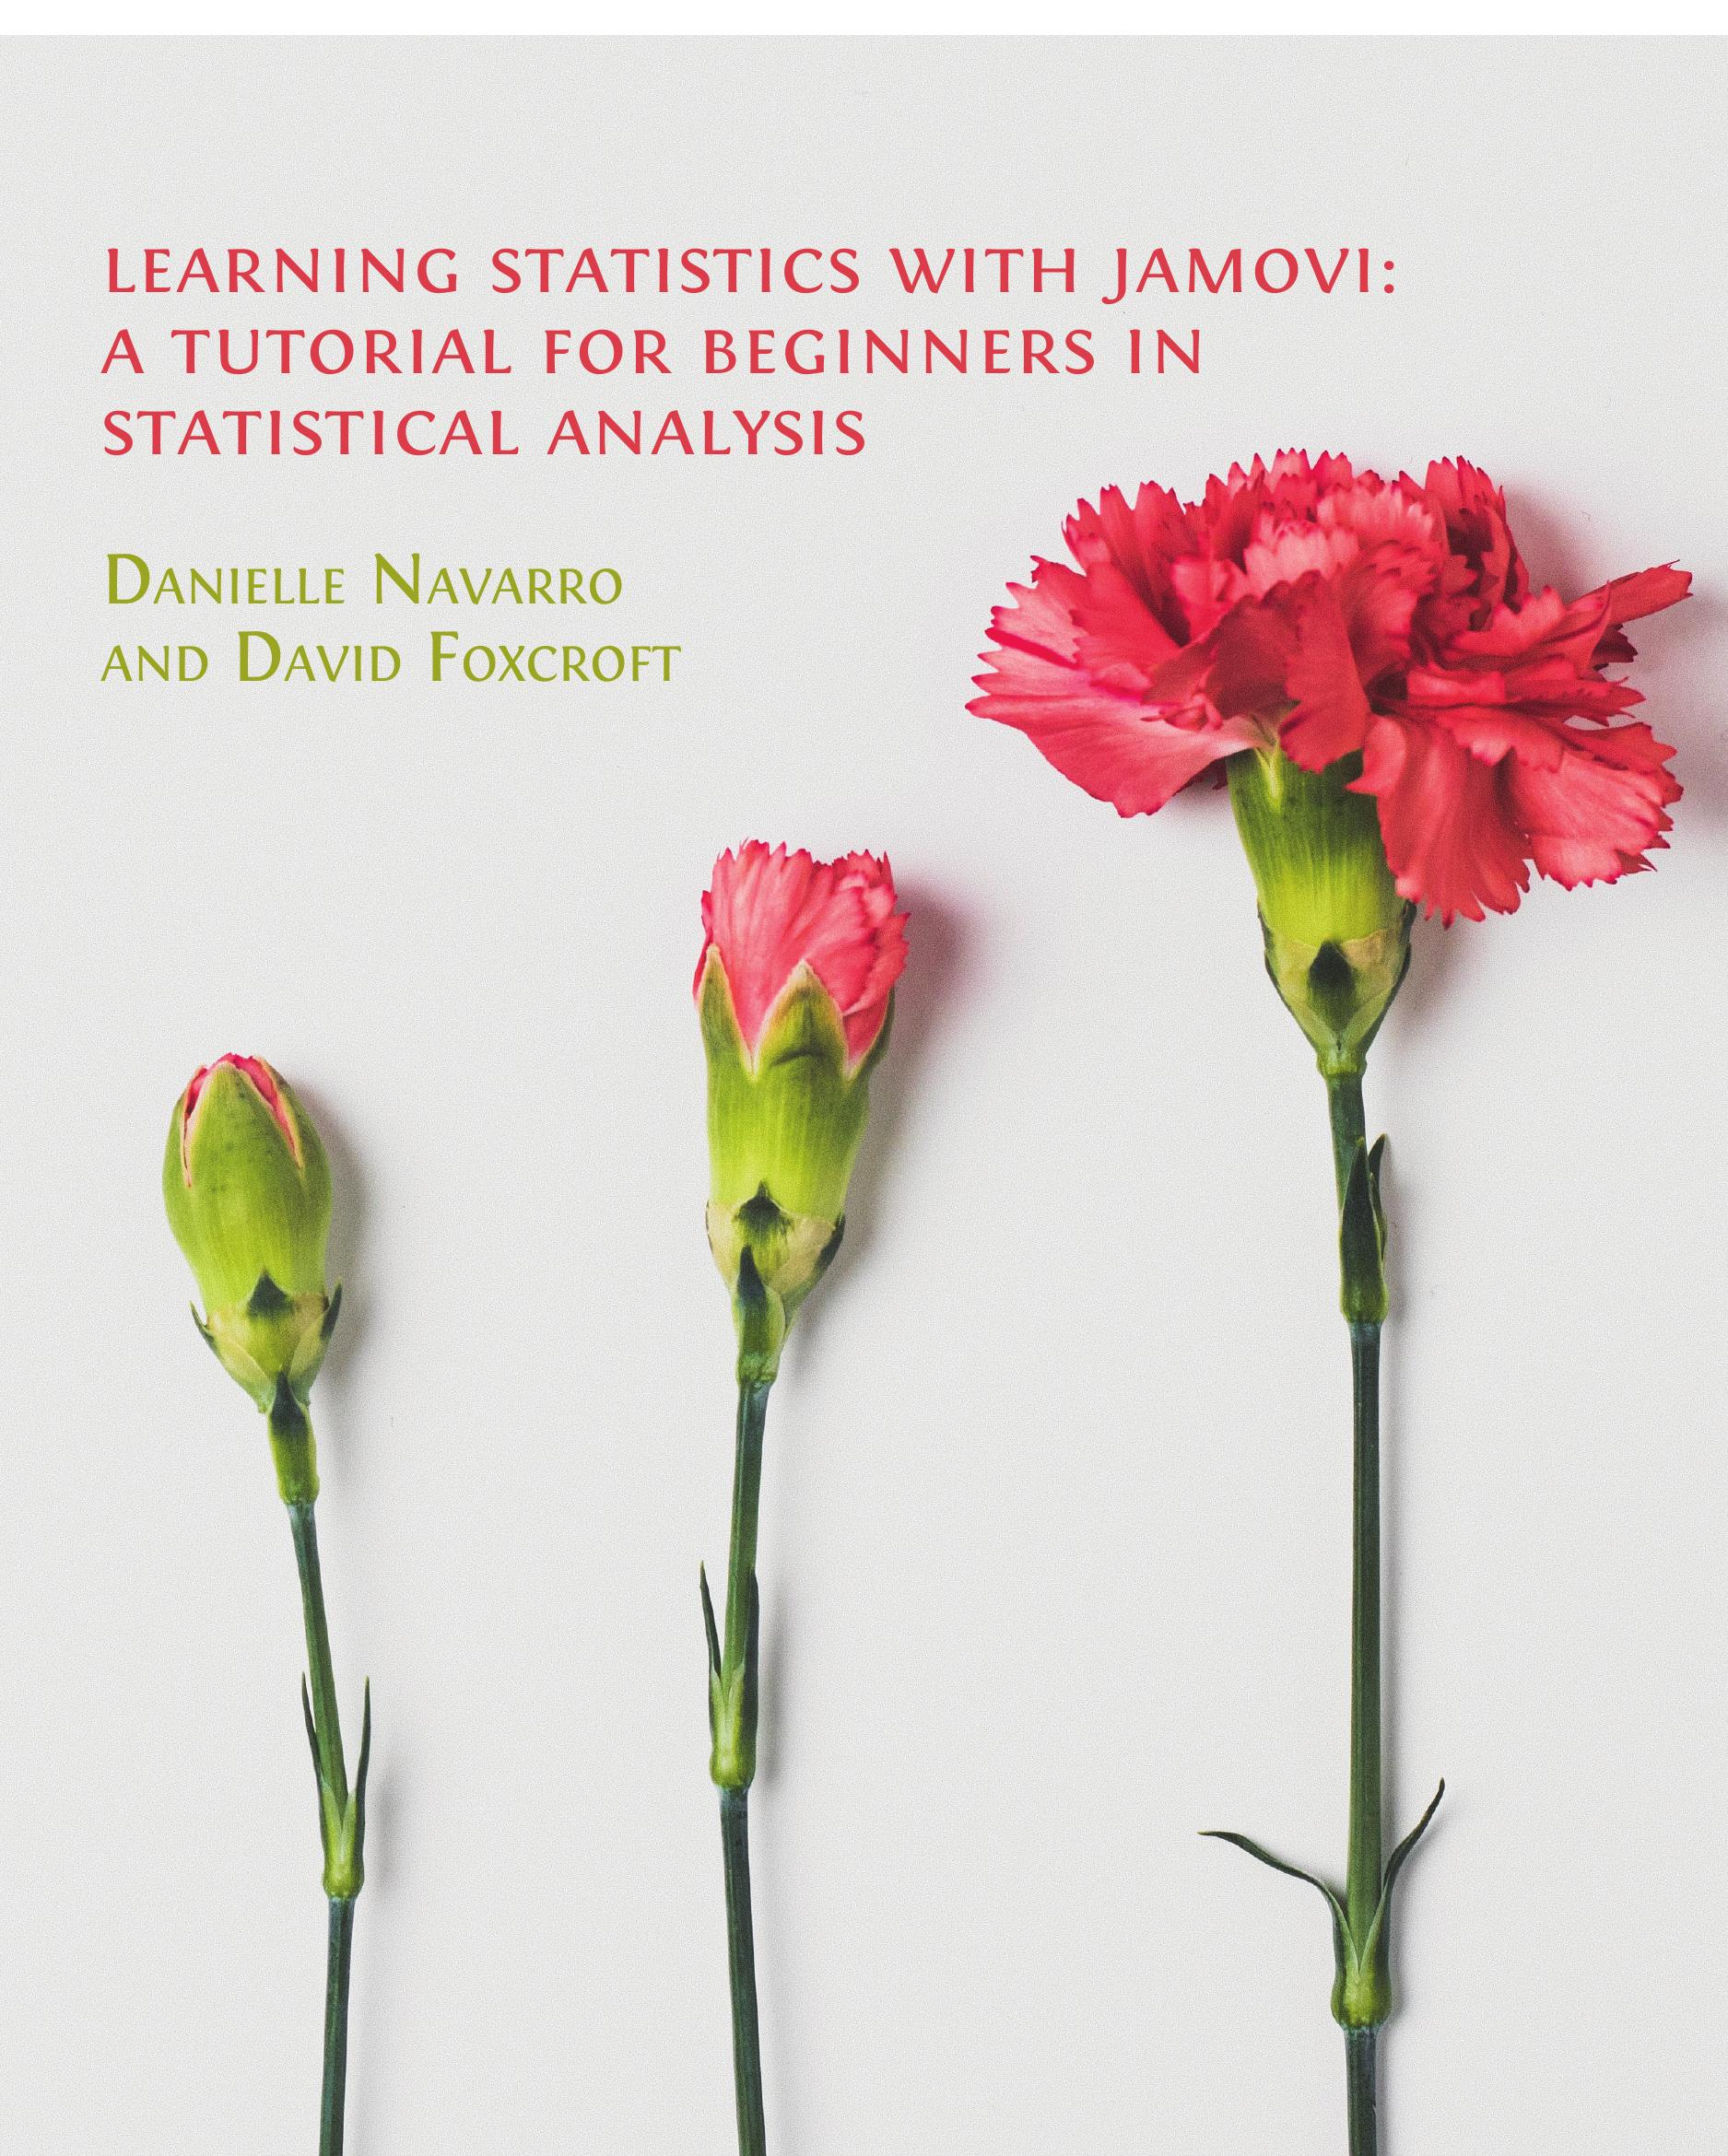
\includepdf[fitpaper=true,pages=-]{images/obp.0333}
\end{center}
\pagestyle{empty}
\let\maketitle\oldmaketitle
\maketitle
\mainmatter
%\pagestyle{plain}
\let\footnote=\endnote

\pagenumbering{roman}
\hspace{0pt}
\vfill
\begin{center}

\Huge{Learning Statistics with jamovi}

\Large{A Tutorial for Beginners in Statistical Analysis}\\*[20pt]

\normalsize{Danielle Navarro and David Foxcroft}

\vfill
\end{center}
\hspace{0pt}
\pagebreak

\hspace{0pt}
\vfill

\copyright 2025 David Foxcroft and Danielle Navarro

This work is licensed under an Attribution-ShareAlike 4.0 International (CC BY-SA 4.0).

This license allows you to copy and redistribute, transform, and build upon the material for any purpose, even commercially. providing attribution is made to the authors (but not in any way that suggests that they endorse you or your use of the work). Attribution should include the following information:

Danielle Navarro and David Foxcroft, \textit{Learning statistics with jamovi: A tutorial for beginners in statistical analysis}. Cambridge, UK: Open Book Publishers, 2025, \url{https://doi.org/10.11647/OBP.0333}

Further details about CC BY-SA licenses are available at \\ \url{https://creativecommons.org/licenses/by-sa/4.0/}

All external links were active at the time of publication unless otherwise stated and have been archived via the Internet Archive Wayback Machine at \\ \url{https://archive.org/web}

Digital material and resources associated with this volume are available at \\ \url{https://doi.org/10.11647/OBP.0333\#resources}

ISBN Paperback: 978-1-80064-937-8

ISBN Hardback: 978-1-80064-938-5

ISBN Digital (PDF): 978-1-80064-939-2

DOI: 10.11647/OBP.0333


\vfill
\hspace{0pt}
\pagebreak

\hspace{0pt}
\vfill

This textbook covers the contents of an introductory statistics class, as typically taught to undergraduate psychology, health or social science students. The book covers how to get started in jamovi as well as giving an introduction to data manipulation. From a statistical perspective, the book discusses descriptive statistics and graphing first, followed by chapters on probability theory, sampling and estimation, and null hypothesis testing. After introducing the theory, the book covers the analysis of contingency tables, correlation, \textit{t}-tests, regression, ANOVA and factor analysis. Bayesian statistics are touched on at the end of the book.

Data sets used in the book are freely available for use in jamovi. All the data files you need can be accessed within jamovi via an add-on module in the jamovi library. Or you can download the files from \url{https://www.learnstatswithjamovi.com}.


Citation: Danielle Navarro and David Foxcroft, \textit{Learning statistics with jamovi: A tutorial for beginners in statistical analysis}. Cambridge, UK: Open Book Publishers, 2025, \url{https://doi.org/10.11647/OBP.0333}

\vfill
\hspace{0pt}

\ifdefined\Shaded\renewenvironment{Shaded}{\begin{tcolorbox}[breakable, enhanced, interior hidden, sharp corners, borderline west={3pt}{0pt}{shadecolor}, boxrule=0pt, frame hidden]}{\end{tcolorbox}}\fi

\renewcommand*\contentsname{Table of contents}
{
\hypersetup{linkcolor=}
\setcounter{tocdepth}{2}
\tableofcontents
}
\mainmatter
\bookmarksetup{startatroot}

\hypertarget{preface}{%
\chapter*{Preface}\label{preface}}
\addcontentsline{toc}{chapter}{Preface}

\markboth{Preface}{Preface}

This book is an adaptation of DJ Navarro (2018). Learning statistics
with R: A tutorial for psychology students and other beginners. (Version
0.6). \url{https://learningstatisticswithr.com/}.

The jamovi version of this book was first released in 2018, as version
0.65. Versions 0.70 and 0.75 were released in subsequent years with
corrections and additions. Details of the changes in all versions of the
book can be found in the original preface which can be found in version
0.7, here: In that time, many people have contacted us asking for a hard
copy version of the book. To achieve this, and to preserve the open
source attributes of the book and materials, we have worked with
\href{https://www.openbookpublishers.com/books/10.11647/obp.0333}{Open
Book Publishers} in Cambridge, UK, to release this updated version. Open
Book Publishers are the leading independent open access publisher of
academic research in the Humanities and Social Sciences in the UK. They
are award-winning, not-for-profit, run by scholars, and committed to
making high-quality research freely available to readers around the
world.

\emph{David Foxcroft\\
January 1st, 2025}

\part{Statistical tools}

\hypertarget{sec-Factorial-ANOVA}{%
\chapter{Factorial ANOVA}\label{sec-Factorial-ANOVA}}

Over the course of the last few chapters we have done quite a lot. We
have looked at statistical tests you can use when you have one nominal
predictor variable with two groups (e.g.~the \(t\)-test in
\textbf{?@sec-Comparing-two-means}) or with three or more groups
(\textbf{?@sec-Comparing-several-means-one-way-ANOVA}).
\textbf{?@sec-Correlation-and-linear-regression} introduced a powerful
new idea, that is building statistical models with multiple continuous
predictor variables used to explain a single outcome variable. For
instance, a regression model could be used to predict the number of
errors a student makes in a reading comprehension test based on the
number of hours they studied for the test and their score on a
standardised IQ test.

The goal in this chapter is to extend the idea of using multiple
predictors into the ANOVA framework. For instance, suppose we were
interested in using the reading comprehension test to measure student
achievements in three different schools, and we suspect that girls and
boys are developing at different rates (and so would be expected to have
different performance on average). Each student is classified in two
different ways: on the basis of their gender and on the basis of their
school. What we'd like to do is analyse the reading comprehension scores
in terms of both of these grouping variables. The tool for doing so is
generically referred to as \textbf{factorial ANOVA}. However, since we
have two grouping variables, we sometimes refer to the analysis as a
two-way ANOVA, in contrast to the one-way ANOVAs that we ran in
\textbf{?@sec-Comparing-several-means-one-way-ANOVA}.

\hypertarget{factorial-anova-1-balanced-designs-focus-on-main-effects}{%
\section{Factorial ANOVA 1: balanced designs, focus on main
effects}\label{factorial-anova-1-balanced-designs-focus-on-main-effects}}

When we discussed analysis of variance in
\textbf{?@sec-Comparing-several-means-one-way-ANOVA}, we assumed a
fairly simple experimental design. Each person is in one of several
groups and we want to know whether these groups have different mean
scores on some outcome variable. In this section, I'll discuss a broader
class of experimental designs known as \textbf{factorial designs}, in
which we have more than one grouping variable. I gave one example of how
this kind of design might arise above. Another example appears in
\textbf{?@sec-Comparing-several-means-one-way-ANOVA} in which we were
looking at the effect of different drugs on the mood.gain experienced by
each person. In that chapter we did find a significant effect of drug,
but at the end of the chapter we also ran an analysis to see if there
was an effect of therapy. We didn't find one, but there's something a
bit worrying about trying to run two separate analyses trying to predict
the same outcome. Maybe there actually is an effect of therapy on mood
gain, but we couldn't find it because it was being ``hidden'' by the
effect of drug? In other words, we're going to want to run a single
analysis that includes both drug and therapy as predictors. For this
analysis each person is cross-classified by the drug they were given (a
factor with 3 levels) and what therapy they received (a factor with 2
levels). We refer to this as a \(3 \times 2\) factorial design.

If we cross-tabulate drug by therapy, using the `Frequencies' -
`Contingency Tables' analysis in jamovi (see
\textbf{?@sec-Tabulating-and-cross-tabulating-data}), we get the table
shown in Figure~\ref{fig-fig14-1}.

\begin{figure}

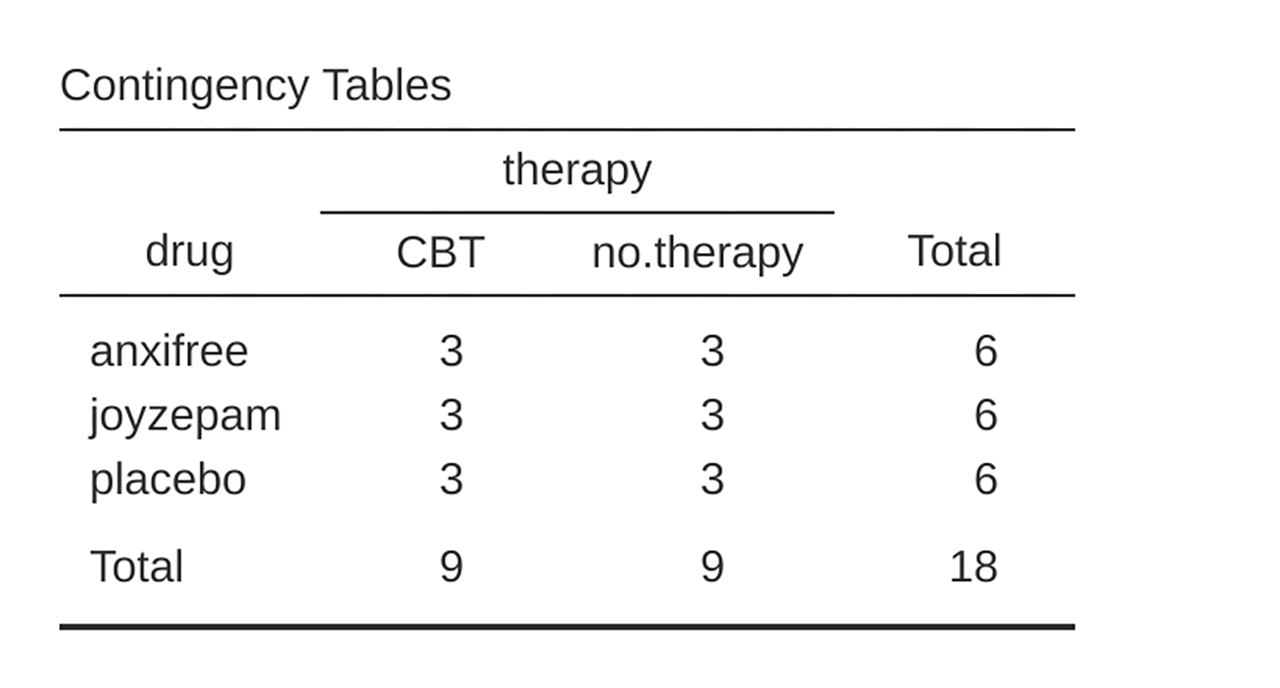
\includegraphics[width=1\textwidth,height=\textheight]{images/fig14-1.png} \hfill{}

\caption{\label{fig-fig14-1}jamovi contingency table of drug by therapy}

\end{figure}

As you can see, not only do we have participants corresponding to all
possible combinations of the two factors, indicating that our design is
\textbf{completely crossed}, it turns out that there are an equal number
of people in each group. In other words, we have a balanced design. In
this section I'll talk about how to analyse data from \textbf{balanced}
designs, since this is the simplest case. The story for unbalanced
designs is quite tedious, so we'll put it to one side for the moment.

\hypertarget{sec-What-hypotheses-are-we-testing}{%
\subsection{What hypotheses are we
testing?}\label{sec-What-hypotheses-are-we-testing}}

Like one-way ANOVA, factorial ANOVA is a tool for testing certain types
of hypotheses about population means. So a sensible place to start would
be to be explicit about what our hypotheses actually are. However,
before we can even get to that point, it's really useful to have some
clean and simple notation to describe the population means. Because of
the fact that observations are cross-classified in terms of two
different factors, there are quite a lot of different means that one
might be interested in. To see this, let's start by thinking about all
the different sample means that we can calculate for this kind of
design. Firstly, there's the obvious idea that we might be interested in
this list of group means (Table~\ref{tbl-tab14-1}).

\hypertarget{tbl-tab14-1}{}
 
  \providecommand{\huxb}[2]{\arrayrulecolor[RGB]{#1}\global\arrayrulewidth=#2pt}
  \providecommand{\huxvb}[2]{\color[RGB]{#1}\vrule width #2pt}
  \providecommand{\huxtpad}[1]{\rule{0pt}{#1}}
  \providecommand{\huxbpad}[1]{\rule[-#1]{0pt}{#1}}

\begin{table}[ht]
\caption{\label{tbl-tab14-1}Group means for drug and therapy groups in the \emph{clinicaltrial.csv}
data }\tabularnewline

\begin{centerbox}
\begin{threeparttable}
\setlength{\tabcolsep}{0pt}
\begin{tabularx}{0.9\textwidth}{p{0.3\textwidth} p{0.3\textwidth} p{0.3\textwidth}}


\hhline{>{\huxb{0, 0, 0}{0.4}}->{\huxb{0, 0, 0}{0.4}}->{\huxb{0, 0, 0}{0.4}}-}
\arrayrulecolor{black}

\multicolumn{1}{!{\huxvb{0, 0, 0}{0}}p{0.3\textwidth}!{\huxvb{0, 0, 0}{0}}}{\hspace{0pt}\parbox[b]{0.3\textwidth-0pt-12pt}{\huxtpad{2pt + 1em}\centering \textbf{drug}\huxbpad{2pt}}} &
\multicolumn{1}{p{0.3\textwidth}!{\huxvb{0, 0, 0}{0}}}{\hspace{12pt}\parbox[b]{0.3\textwidth-12pt-12pt}{\huxtpad{2pt + 1em}\centering \textbf{therapy}\huxbpad{2pt}}} &
\multicolumn{1}{p{0.3\textwidth}!{\huxvb{0, 0, 0}{0}}}{\hspace{12pt}\parbox[b]{0.3\textwidth-12pt-0pt}{\huxtpad{2pt + 1em}\centering \textbf{mood.gain}\huxbpad{2pt}}} \tabularnewline[-0.5pt]


\hhline{>{\huxb{0, 0, 0}{0.4}}->{\huxb{0, 0, 0}{0.4}}->{\huxb{0, 0, 0}{0.4}}-}
\arrayrulecolor{black}

\multicolumn{1}{!{\huxvb{0, 0, 0}{0}}p{0.3\textwidth}!{\huxvb{0, 0, 0}{0}}}{\hspace{0pt}\parbox[b]{0.3\textwidth-0pt-12pt}{\huxtpad{2pt + 1em}\centering placebo\huxbpad{2pt}}} &
\multicolumn{1}{p{0.3\textwidth}!{\huxvb{0, 0, 0}{0}}}{\hspace{12pt}\parbox[b]{0.3\textwidth-12pt-12pt}{\huxtpad{2pt + 1em}\centering no.therapy\huxbpad{2pt}}} &
\multicolumn{1}{p{0.3\textwidth}!{\huxvb{0, 0, 0}{0}}}{\hspace{12pt}\parbox[b]{0.3\textwidth-12pt-0pt}{\huxtpad{2pt + 1em}\centering 0.30\huxbpad{2pt}}} \tabularnewline[-0.5pt]


\hhline{}
\arrayrulecolor{black}

\multicolumn{1}{!{\huxvb{0, 0, 0}{0}}p{0.3\textwidth}!{\huxvb{0, 0, 0}{0}}}{\hspace{0pt}\parbox[b]{0.3\textwidth-0pt-12pt}{\huxtpad{2pt + 1em}\centering anxifree\huxbpad{2pt}}} &
\multicolumn{1}{p{0.3\textwidth}!{\huxvb{0, 0, 0}{0}}}{\hspace{12pt}\parbox[b]{0.3\textwidth-12pt-12pt}{\huxtpad{2pt + 1em}\centering no.therapy\huxbpad{2pt}}} &
\multicolumn{1}{p{0.3\textwidth}!{\huxvb{0, 0, 0}{0}}}{\hspace{12pt}\parbox[b]{0.3\textwidth-12pt-0pt}{\huxtpad{2pt + 1em}\centering 0.40\huxbpad{2pt}}} \tabularnewline[-0.5pt]


\hhline{}
\arrayrulecolor{black}

\multicolumn{1}{!{\huxvb{0, 0, 0}{0}}p{0.3\textwidth}!{\huxvb{0, 0, 0}{0}}}{\hspace{0pt}\parbox[b]{0.3\textwidth-0pt-12pt}{\huxtpad{2pt + 1em}\centering joyzepam\huxbpad{2pt}}} &
\multicolumn{1}{p{0.3\textwidth}!{\huxvb{0, 0, 0}{0}}}{\hspace{12pt}\parbox[b]{0.3\textwidth-12pt-12pt}{\huxtpad{2pt + 1em}\centering no.therapy\huxbpad{2pt}}} &
\multicolumn{1}{p{0.3\textwidth}!{\huxvb{0, 0, 0}{0}}}{\hspace{12pt}\parbox[b]{0.3\textwidth-12pt-0pt}{\huxtpad{2pt + 1em}\centering 1.47\huxbpad{2pt}}} \tabularnewline[-0.5pt]


\hhline{}
\arrayrulecolor{black}

\multicolumn{1}{!{\huxvb{0, 0, 0}{0}}p{0.3\textwidth}!{\huxvb{0, 0, 0}{0}}}{\hspace{0pt}\parbox[b]{0.3\textwidth-0pt-12pt}{\huxtpad{2pt + 1em}\centering placebo\huxbpad{2pt}}} &
\multicolumn{1}{p{0.3\textwidth}!{\huxvb{0, 0, 0}{0}}}{\hspace{12pt}\parbox[b]{0.3\textwidth-12pt-12pt}{\huxtpad{2pt + 1em}\centering CBT\huxbpad{2pt}}} &
\multicolumn{1}{p{0.3\textwidth}!{\huxvb{0, 0, 0}{0}}}{\hspace{12pt}\parbox[b]{0.3\textwidth-12pt-0pt}{\huxtpad{2pt + 1em}\centering 0.60\huxbpad{2pt}}} \tabularnewline[-0.5pt]


\hhline{}
\arrayrulecolor{black}

\multicolumn{1}{!{\huxvb{0, 0, 0}{0}}p{0.3\textwidth}!{\huxvb{0, 0, 0}{0}}}{\hspace{0pt}\parbox[b]{0.3\textwidth-0pt-12pt}{\huxtpad{2pt + 1em}\centering anxifree\huxbpad{2pt}}} &
\multicolumn{1}{p{0.3\textwidth}!{\huxvb{0, 0, 0}{0}}}{\hspace{12pt}\parbox[b]{0.3\textwidth-12pt-12pt}{\huxtpad{2pt + 1em}\centering CBT\huxbpad{2pt}}} &
\multicolumn{1}{p{0.3\textwidth}!{\huxvb{0, 0, 0}{0}}}{\hspace{12pt}\parbox[b]{0.3\textwidth-12pt-0pt}{\huxtpad{2pt + 1em}\centering 1.03\huxbpad{2pt}}} \tabularnewline[-0.5pt]


\hhline{}
\arrayrulecolor{black}

\multicolumn{1}{!{\huxvb{0, 0, 0}{0}}p{0.3\textwidth}!{\huxvb{0, 0, 0}{0}}}{\hspace{0pt}\parbox[b]{0.3\textwidth-0pt-12pt}{\huxtpad{2pt + 1em}\centering joyzepam\huxbpad{2pt}}} &
\multicolumn{1}{p{0.3\textwidth}!{\huxvb{0, 0, 0}{0}}}{\hspace{12pt}\parbox[b]{0.3\textwidth-12pt-12pt}{\huxtpad{2pt + 1em}\centering CBT\huxbpad{2pt}}} &
\multicolumn{1}{p{0.3\textwidth}!{\huxvb{0, 0, 0}{0}}}{\hspace{12pt}\parbox[b]{0.3\textwidth-12pt-0pt}{\huxtpad{2pt + 1em}\centering 1.50\huxbpad{2pt}}} \tabularnewline[-0.5pt]


\hhline{>{\huxb{0, 0, 0}{0.4}}->{\huxb{0, 0, 0}{0.4}}->{\huxb{0, 0, 0}{0.4}}-}
\arrayrulecolor{black}
\end{tabularx} 

\end{threeparttable}\par\end{centerbox}

\end{table}
 

Now, the next Table (Table~\ref{tbl-tab14-2}) shows a list of the group
means for all possible combinations of the two factors (e.g., people who
received the placebo and no therapy, people who received the placebo
while getting CBT, etc.). It is helpful to organise all these numbers,
plus the marginal and grand means, into a single table which looks like
this:

\hypertarget{tbl-tab14-2}{}
 
  \providecommand{\huxb}[2]{\arrayrulecolor[RGB]{#1}\global\arrayrulewidth=#2pt}
  \providecommand{\huxvb}[2]{\color[RGB]{#1}\vrule width #2pt}
  \providecommand{\huxtpad}[1]{\rule{0pt}{#1}}
  \providecommand{\huxbpad}[1]{\rule[-#1]{0pt}{#1}}

\begin{table}[ht]
\caption{\label{tbl-tab14-2}Group and total means for drug and therapy groups in the
\emph{clinicaltrial.csv} data }\tabularnewline

\begin{centerbox}
\begin{threeparttable}
\setlength{\tabcolsep}{0pt}
\begin{tabularx}{0.9\textwidth}{p{0.225\textwidth} p{0.225\textwidth} p{0.225\textwidth} p{0.225\textwidth}}


\hhline{>{\huxb{0, 0, 0}{0.4}}->{\huxb{0, 0, 0}{0.4}}->{\huxb{0, 0, 0}{0.4}}->{\huxb{0, 0, 0}{0.4}}-}
\arrayrulecolor{black}

\multicolumn{1}{!{\huxvb{0, 0, 0}{0}}p{0.225\textwidth}!{\huxvb{0, 0, 0}{0}}}{\hspace{0pt}\parbox[b]{0.225\textwidth-0pt-12pt}{\huxtpad{2pt + 1em}\centering \textbf{}\huxbpad{2pt}}} &
\multicolumn{1}{p{0.225\textwidth}!{\huxvb{0, 0, 0}{0}}}{\hspace{12pt}\parbox[b]{0.225\textwidth-12pt-12pt}{\huxtpad{2pt + 1em}\centering \textbf{no therapy}\huxbpad{2pt}}} &
\multicolumn{1}{p{0.225\textwidth}!{\huxvb{0, 0, 0}{0}}}{\hspace{12pt}\parbox[b]{0.225\textwidth-12pt-12pt}{\huxtpad{2pt + 1em}\centering \textbf{CBT}\huxbpad{2pt}}} &
\multicolumn{1}{p{0.225\textwidth}!{\huxvb{0, 0, 0}{0}}}{\hspace{12pt}\parbox[b]{0.225\textwidth-12pt-0pt}{\huxtpad{2pt + 1em}\centering \textbf{total}\huxbpad{2pt}}} \tabularnewline[-0.5pt]


\hhline{>{\huxb{0, 0, 0}{0.4}}->{\huxb{0, 0, 0}{0.4}}->{\huxb{0, 0, 0}{0.4}}->{\huxb{0, 0, 0}{0.4}}-}
\arrayrulecolor{black}

\multicolumn{1}{!{\huxvb{0, 0, 0}{0}}p{0.225\textwidth}!{\huxvb{0, 0, 0}{0}}}{\hspace{0pt}\parbox[b]{0.225\textwidth-0pt-12pt}{\huxtpad{2pt + 1em}\centering placebo\huxbpad{2pt}}} &
\multicolumn{1}{p{0.225\textwidth}!{\huxvb{0, 0, 0}{0}}}{\hspace{12pt}\parbox[b]{0.225\textwidth-12pt-12pt}{\huxtpad{2pt + 1em}\centering 0.30\huxbpad{2pt}}} &
\multicolumn{1}{p{0.225\textwidth}!{\huxvb{0, 0, 0}{0}}}{\hspace{12pt}\parbox[b]{0.225\textwidth-12pt-12pt}{\huxtpad{2pt + 1em}\centering 0.60\huxbpad{2pt}}} &
\multicolumn{1}{p{0.225\textwidth}!{\huxvb{0, 0, 0}{0}}}{\hspace{12pt}\parbox[b]{0.225\textwidth-12pt-0pt}{\huxtpad{2pt + 1em}\centering 0.45\huxbpad{2pt}}} \tabularnewline[-0.5pt]


\hhline{}
\arrayrulecolor{black}

\multicolumn{1}{!{\huxvb{0, 0, 0}{0}}p{0.225\textwidth}!{\huxvb{0, 0, 0}{0}}}{\hspace{0pt}\parbox[b]{0.225\textwidth-0pt-12pt}{\huxtpad{2pt + 1em}\centering anxifree\huxbpad{2pt}}} &
\multicolumn{1}{p{0.225\textwidth}!{\huxvb{0, 0, 0}{0}}}{\hspace{12pt}\parbox[b]{0.225\textwidth-12pt-12pt}{\huxtpad{2pt + 1em}\centering 0.40\huxbpad{2pt}}} &
\multicolumn{1}{p{0.225\textwidth}!{\huxvb{0, 0, 0}{0}}}{\hspace{12pt}\parbox[b]{0.225\textwidth-12pt-12pt}{\huxtpad{2pt + 1em}\centering 1.03\huxbpad{2pt}}} &
\multicolumn{1}{p{0.225\textwidth}!{\huxvb{0, 0, 0}{0}}}{\hspace{12pt}\parbox[b]{0.225\textwidth-12pt-0pt}{\huxtpad{2pt + 1em}\centering 0.72\huxbpad{2pt}}} \tabularnewline[-0.5pt]


\hhline{}
\arrayrulecolor{black}

\multicolumn{1}{!{\huxvb{0, 0, 0}{0}}p{0.225\textwidth}!{\huxvb{0, 0, 0}{0}}}{\hspace{0pt}\parbox[b]{0.225\textwidth-0pt-12pt}{\huxtpad{2pt + 1em}\centering joyzepam\huxbpad{2pt}}} &
\multicolumn{1}{p{0.225\textwidth}!{\huxvb{0, 0, 0}{0}}}{\hspace{12pt}\parbox[b]{0.225\textwidth-12pt-12pt}{\huxtpad{2pt + 1em}\centering 1.47\huxbpad{2pt}}} &
\multicolumn{1}{p{0.225\textwidth}!{\huxvb{0, 0, 0}{0}}}{\hspace{12pt}\parbox[b]{0.225\textwidth-12pt-12pt}{\huxtpad{2pt + 1em}\centering 1.50\huxbpad{2pt}}} &
\multicolumn{1}{p{0.225\textwidth}!{\huxvb{0, 0, 0}{0}}}{\hspace{12pt}\parbox[b]{0.225\textwidth-12pt-0pt}{\huxtpad{2pt + 1em}\centering 1.48\huxbpad{2pt}}} \tabularnewline[-0.5pt]


\hhline{}
\arrayrulecolor{black}

\multicolumn{1}{!{\huxvb{0, 0, 0}{0}}p{0.225\textwidth}!{\huxvb{0, 0, 0}{0}}}{\hspace{0pt}\parbox[b]{0.225\textwidth-0pt-12pt}{\huxtpad{2pt + 1em}\centering total\huxbpad{2pt}}} &
\multicolumn{1}{p{0.225\textwidth}!{\huxvb{0, 0, 0}{0}}}{\hspace{12pt}\parbox[b]{0.225\textwidth-12pt-12pt}{\huxtpad{2pt + 1em}\centering 0.72\huxbpad{2pt}}} &
\multicolumn{1}{p{0.225\textwidth}!{\huxvb{0, 0, 0}{0}}}{\hspace{12pt}\parbox[b]{0.225\textwidth-12pt-12pt}{\huxtpad{2pt + 1em}\centering 1.04\huxbpad{2pt}}} &
\multicolumn{1}{p{0.225\textwidth}!{\huxvb{0, 0, 0}{0}}}{\hspace{12pt}\parbox[b]{0.225\textwidth-12pt-0pt}{\huxtpad{2pt + 1em}\centering 0.88\huxbpad{2pt}}} \tabularnewline[-0.5pt]


\hhline{>{\huxb{0, 0, 0}{0.4}}->{\huxb{0, 0, 0}{0.4}}->{\huxb{0, 0, 0}{0.4}}->{\huxb{0, 0, 0}{0.4}}-}
\arrayrulecolor{black}
\end{tabularx} 

\end{threeparttable}\par\end{centerbox}

\end{table}
 

Now, each of these different means is of course a sample statistic. It's
a quantity that pertains to the specific observations that we've made
during our study. What we want to make inferences about are the
corresponding population parameters. That is, the true means as they
exist within some broader population. Those population means can also be
organised into a similar table, but we'll need a little mathematical
notation to do so (Table~\ref{tbl-tab14-3}). As usual, I'll use the
symbol \(\mu\) to denote a population mean. However, because there are
lots of different means, I'll need to use subscripts to distinguish
between them.

Here's how the notation works. Our table is defined in terms of two
factors. Each row corresponds to a different level of Factor A (in this
case drug), and each column corresponds to a different level of Factor B
(in this case therapy). If we let \(R\) denote the number of rows in the
table, and \(C\) denote the number of columns, we can refer to this as
an \(R \times C\) factorial ANOVA. In this case \(R = 3\) and \(C = 2\).
We'll use lowercase letters to refer to specific rows and columns, so
\(\mu_{rc}\) refers to the population mean associated with the \(r\)-th
level of Factor A (i.e.~row number \(r\)) and the \(c\)-th level of
Factor B (column number c).\footnote{The nice thing about the subscript
  notation is that it generalises nicely. If our experiment had involved
  a third factor, then we could just add a third subscript. In
  principle, the notation extends to as many factors as you might care
  to include, but in this book we'll rarely consider analyses involving
  more than two factors, and never more than three.} So the population
means are now written like in Table~\ref{tbl-tab14-1}:

\hypertarget{tbl-tab14-3}{}
 
  \providecommand{\huxb}[2]{\arrayrulecolor[RGB]{#1}\global\arrayrulewidth=#2pt}
  \providecommand{\huxvb}[2]{\color[RGB]{#1}\vrule width #2pt}
  \providecommand{\huxtpad}[1]{\rule{0pt}{#1}}
  \providecommand{\huxbpad}[1]{\rule[-#1]{0pt}{#1}}

\begin{table}[ht]
\caption{\label{tbl-tab14-3}Notation for population means in a factorial table }\tabularnewline

\begin{centerbox}
\begin{threeparttable}
\setlength{\tabcolsep}{0pt}
\begin{tabularx}{0.9\textwidth}{p{0.225\textwidth} p{0.225\textwidth} p{0.225\textwidth} p{0.225\textwidth}}


\hhline{>{\huxb{0, 0, 0}{0.4}}->{\huxb{0, 0, 0}{0.4}}->{\huxb{0, 0, 0}{0.4}}->{\huxb{0, 0, 0}{0.4}}-}
\arrayrulecolor{black}

\multicolumn{1}{!{\huxvb{0, 0, 0}{0}}p{0.225\textwidth}!{\huxvb{0, 0, 0}{0}}}{\hspace{0pt}\parbox[b]{0.225\textwidth-0pt-12pt}{\huxtpad{2pt + 1em}\centering \textbf{}\huxbpad{2pt}}} &
\multicolumn{1}{p{0.225\textwidth}!{\huxvb{0, 0, 0}{0}}}{\hspace{12pt}\parbox[b]{0.225\textwidth-12pt-12pt}{\huxtpad{2pt + 1em}\centering \textbf{no therapy}\huxbpad{2pt}}} &
\multicolumn{1}{p{0.225\textwidth}!{\huxvb{0, 0, 0}{0}}}{\hspace{12pt}\parbox[b]{0.225\textwidth-12pt-12pt}{\huxtpad{2pt + 1em}\centering \textbf{CBT}\huxbpad{2pt}}} &
\multicolumn{1}{p{0.225\textwidth}!{\huxvb{0, 0, 0}{0}}}{\hspace{12pt}\parbox[b]{0.225\textwidth-12pt-0pt}{\huxtpad{2pt + 1em}\centering \textbf{total}\huxbpad{2pt}}} \tabularnewline[-0.5pt]


\hhline{>{\huxb{0, 0, 0}{0.4}}->{\huxb{0, 0, 0}{0.4}}->{\huxb{0, 0, 0}{0.4}}->{\huxb{0, 0, 0}{0.4}}-}
\arrayrulecolor{black}

\multicolumn{1}{!{\huxvb{0, 0, 0}{0}}p{0.225\textwidth}!{\huxvb{0, 0, 0}{0}}}{\hspace{0pt}\parbox[b]{0.225\textwidth-0pt-12pt}{\huxtpad{2pt + 1em}\centering placebo\huxbpad{2pt}}} &
\multicolumn{1}{p{0.225\textwidth}!{\huxvb{0, 0, 0}{0}}}{\hspace{12pt}\parbox[b]{0.225\textwidth-12pt-12pt}{\huxtpad{2pt + 1em}\centering \( \mu_{11} \)\huxbpad{2pt}}} &
\multicolumn{1}{p{0.225\textwidth}!{\huxvb{0, 0, 0}{0}}}{\hspace{12pt}\parbox[b]{0.225\textwidth-12pt-12pt}{\huxtpad{2pt + 1em}\centering \( \mu_{12} \)\huxbpad{2pt}}} &
\multicolumn{1}{p{0.225\textwidth}!{\huxvb{0, 0, 0}{0}}}{\hspace{12pt}\parbox[b]{0.225\textwidth-12pt-0pt}{\huxtpad{2pt + 1em}\centering \huxbpad{2pt}}} \tabularnewline[-0.5pt]


\hhline{}
\arrayrulecolor{black}

\multicolumn{1}{!{\huxvb{0, 0, 0}{0}}p{0.225\textwidth}!{\huxvb{0, 0, 0}{0}}}{\hspace{0pt}\parbox[b]{0.225\textwidth-0pt-12pt}{\huxtpad{2pt + 1em}\centering anxifree\huxbpad{2pt}}} &
\multicolumn{1}{p{0.225\textwidth}!{\huxvb{0, 0, 0}{0}}}{\hspace{12pt}\parbox[b]{0.225\textwidth-12pt-12pt}{\huxtpad{2pt + 1em}\centering \( \mu_{21} \)\huxbpad{2pt}}} &
\multicolumn{1}{p{0.225\textwidth}!{\huxvb{0, 0, 0}{0}}}{\hspace{12pt}\parbox[b]{0.225\textwidth-12pt-12pt}{\huxtpad{2pt + 1em}\centering \( \mu_{22} \)\huxbpad{2pt}}} &
\multicolumn{1}{p{0.225\textwidth}!{\huxvb{0, 0, 0}{0}}}{\hspace{12pt}\parbox[b]{0.225\textwidth-12pt-0pt}{\huxtpad{2pt + 1em}\centering \huxbpad{2pt}}} \tabularnewline[-0.5pt]


\hhline{}
\arrayrulecolor{black}

\multicolumn{1}{!{\huxvb{0, 0, 0}{0}}p{0.225\textwidth}!{\huxvb{0, 0, 0}{0}}}{\hspace{0pt}\parbox[b]{0.225\textwidth-0pt-12pt}{\huxtpad{2pt + 1em}\centering joyzepam\huxbpad{2pt}}} &
\multicolumn{1}{p{0.225\textwidth}!{\huxvb{0, 0, 0}{0}}}{\hspace{12pt}\parbox[b]{0.225\textwidth-12pt-12pt}{\huxtpad{2pt + 1em}\centering \( \mu_{31} \)\huxbpad{2pt}}} &
\multicolumn{1}{p{0.225\textwidth}!{\huxvb{0, 0, 0}{0}}}{\hspace{12pt}\parbox[b]{0.225\textwidth-12pt-12pt}{\huxtpad{2pt + 1em}\centering \( \mu_{32} \)\huxbpad{2pt}}} &
\multicolumn{1}{p{0.225\textwidth}!{\huxvb{0, 0, 0}{0}}}{\hspace{12pt}\parbox[b]{0.225\textwidth-12pt-0pt}{\huxtpad{2pt + 1em}\centering \huxbpad{2pt}}} \tabularnewline[-0.5pt]


\hhline{}
\arrayrulecolor{black}

\multicolumn{1}{!{\huxvb{0, 0, 0}{0}}p{0.225\textwidth}!{\huxvb{0, 0, 0}{0}}}{\hspace{0pt}\parbox[b]{0.225\textwidth-0pt-12pt}{\huxtpad{2pt + 1em}\centering total\huxbpad{2pt}}} &
\multicolumn{1}{p{0.225\textwidth}!{\huxvb{0, 0, 0}{0}}}{\hspace{12pt}\parbox[b]{0.225\textwidth-12pt-12pt}{\huxtpad{2pt + 1em}\centering \huxbpad{2pt}}} &
\multicolumn{1}{p{0.225\textwidth}!{\huxvb{0, 0, 0}{0}}}{\hspace{12pt}\parbox[b]{0.225\textwidth-12pt-12pt}{\huxtpad{2pt + 1em}\centering \huxbpad{2pt}}} &
\multicolumn{1}{p{0.225\textwidth}!{\huxvb{0, 0, 0}{0}}}{\hspace{12pt}\parbox[b]{0.225\textwidth-12pt-0pt}{\huxtpad{2pt + 1em}\centering \huxbpad{2pt}}} \tabularnewline[-0.5pt]


\hhline{>{\huxb{0, 0, 0}{0.4}}->{\huxb{0, 0, 0}{0.4}}->{\huxb{0, 0, 0}{0.4}}->{\huxb{0, 0, 0}{0.4}}-}
\arrayrulecolor{black}
\end{tabularx} 

\end{threeparttable}\par\end{centerbox}

\end{table}
 

Okay, what about the remaining entries? For instance, how should we
describe the average mood gain across the entire (hypothetical)
population of people who might be given Joyzepam in an experiment like
this, regardless of whether they were in CBT? We use the ``dot''
notation to express this. In the case of Joyzepam, notice that we're
talking about the mean associated with the third row in the table. That
is, we're averaging across two cell means (i.e., \(\mu_{31}\) and
\(\mu_{32}\)). The result of this averaging is referred to as a marginal
mean, and would be denoted \(\mu_3.\) in this case. The \textbf{marginal
mean} for CBT corresponds to the population mean associated with the
second column in the table, so we use the notation because it is the
mean obtained by averaging (marginalising)\footnote{Technically,
  marginalising isn't quite identical to a regular mean. It's a weighted
  average where you take into account the frequency of the different
  events that you're averaging over. However, in a balanced design, all
  of our cell frequencies are equal by definition so the two are
  equivalent. We'll discuss unbalanced designs later, and when we do so
  you'll see that all of our calculations become a real headache. But
  let's ignore this for now.} over both. So our full table of population
means can be written down like in Table~\ref{tbl-tab14-4}.

\hypertarget{tbl-tab14-4}{}
 
  \providecommand{\huxb}[2]{\arrayrulecolor[RGB]{#1}\global\arrayrulewidth=#2pt}
  \providecommand{\huxvb}[2]{\color[RGB]{#1}\vrule width #2pt}
  \providecommand{\huxtpad}[1]{\rule{0pt}{#1}}
  \providecommand{\huxbpad}[1]{\rule[-#1]{0pt}{#1}}

\begin{table}[ht]
\caption{\label{tbl-tab14-4}Notation for population and total means in a factorial table }\tabularnewline

\begin{centerbox}
\begin{threeparttable}
\setlength{\tabcolsep}{0pt}
\begin{tabularx}{0.9\textwidth}{p{0.225\textwidth} p{0.225\textwidth} p{0.225\textwidth} p{0.225\textwidth}}


\hhline{>{\huxb{0, 0, 0}{0.4}}->{\huxb{0, 0, 0}{0.4}}->{\huxb{0, 0, 0}{0.4}}->{\huxb{0, 0, 0}{0.4}}-}
\arrayrulecolor{black}

\multicolumn{1}{!{\huxvb{0, 0, 0}{0}}p{0.225\textwidth}!{\huxvb{0, 0, 0}{0}}}{\hspace{0pt}\parbox[b]{0.225\textwidth-0pt-12pt}{\huxtpad{2pt + 1em}\centering \textbf{}\huxbpad{2pt}}} &
\multicolumn{1}{p{0.225\textwidth}!{\huxvb{0, 0, 0}{0}}}{\hspace{12pt}\parbox[b]{0.225\textwidth-12pt-12pt}{\huxtpad{2pt + 1em}\centering \textbf{no therapy}\huxbpad{2pt}}} &
\multicolumn{1}{p{0.225\textwidth}!{\huxvb{0, 0, 0}{0}}}{\hspace{12pt}\parbox[b]{0.225\textwidth-12pt-12pt}{\huxtpad{2pt + 1em}\centering \textbf{CBT}\huxbpad{2pt}}} &
\multicolumn{1}{p{0.225\textwidth}!{\huxvb{0, 0, 0}{0}}}{\hspace{12pt}\parbox[b]{0.225\textwidth-12pt-0pt}{\huxtpad{2pt + 1em}\centering \textbf{total}\huxbpad{2pt}}} \tabularnewline[-0.5pt]


\hhline{>{\huxb{0, 0, 0}{0.4}}->{\huxb{0, 0, 0}{0.4}}->{\huxb{0, 0, 0}{0.4}}->{\huxb{0, 0, 0}{0.4}}-}
\arrayrulecolor{black}

\multicolumn{1}{!{\huxvb{0, 0, 0}{0}}p{0.225\textwidth}!{\huxvb{0, 0, 0}{0}}}{\hspace{0pt}\parbox[b]{0.225\textwidth-0pt-12pt}{\huxtpad{2pt + 1em}\centering placebo\huxbpad{2pt}}} &
\multicolumn{1}{p{0.225\textwidth}!{\huxvb{0, 0, 0}{0}}}{\hspace{12pt}\parbox[b]{0.225\textwidth-12pt-12pt}{\huxtpad{2pt + 1em}\centering \( \mu_{11} \)\huxbpad{2pt}}} &
\multicolumn{1}{p{0.225\textwidth}!{\huxvb{0, 0, 0}{0}}}{\hspace{12pt}\parbox[b]{0.225\textwidth-12pt-12pt}{\huxtpad{2pt + 1em}\centering \( \mu_{12} \)\huxbpad{2pt}}} &
\multicolumn{1}{p{0.225\textwidth}!{\huxvb{0, 0, 0}{0}}}{\hspace{12pt}\parbox[b]{0.225\textwidth-12pt-0pt}{\huxtpad{2pt + 1em}\centering \( \mu_{1.} \)\huxbpad{2pt}}} \tabularnewline[-0.5pt]


\hhline{}
\arrayrulecolor{black}

\multicolumn{1}{!{\huxvb{0, 0, 0}{0}}p{0.225\textwidth}!{\huxvb{0, 0, 0}{0}}}{\hspace{0pt}\parbox[b]{0.225\textwidth-0pt-12pt}{\huxtpad{2pt + 1em}\centering anxifree\huxbpad{2pt}}} &
\multicolumn{1}{p{0.225\textwidth}!{\huxvb{0, 0, 0}{0}}}{\hspace{12pt}\parbox[b]{0.225\textwidth-12pt-12pt}{\huxtpad{2pt + 1em}\centering \( \mu_{21} \)\huxbpad{2pt}}} &
\multicolumn{1}{p{0.225\textwidth}!{\huxvb{0, 0, 0}{0}}}{\hspace{12pt}\parbox[b]{0.225\textwidth-12pt-12pt}{\huxtpad{2pt + 1em}\centering \( \mu_{22} \)\huxbpad{2pt}}} &
\multicolumn{1}{p{0.225\textwidth}!{\huxvb{0, 0, 0}{0}}}{\hspace{12pt}\parbox[b]{0.225\textwidth-12pt-0pt}{\huxtpad{2pt + 1em}\centering \( \mu_{2.} \)\huxbpad{2pt}}} \tabularnewline[-0.5pt]


\hhline{}
\arrayrulecolor{black}

\multicolumn{1}{!{\huxvb{0, 0, 0}{0}}p{0.225\textwidth}!{\huxvb{0, 0, 0}{0}}}{\hspace{0pt}\parbox[b]{0.225\textwidth-0pt-12pt}{\huxtpad{2pt + 1em}\centering joyzepam\huxbpad{2pt}}} &
\multicolumn{1}{p{0.225\textwidth}!{\huxvb{0, 0, 0}{0}}}{\hspace{12pt}\parbox[b]{0.225\textwidth-12pt-12pt}{\huxtpad{2pt + 1em}\centering \( \mu_{31} \)\huxbpad{2pt}}} &
\multicolumn{1}{p{0.225\textwidth}!{\huxvb{0, 0, 0}{0}}}{\hspace{12pt}\parbox[b]{0.225\textwidth-12pt-12pt}{\huxtpad{2pt + 1em}\centering \( \mu_{32} \)\huxbpad{2pt}}} &
\multicolumn{1}{p{0.225\textwidth}!{\huxvb{0, 0, 0}{0}}}{\hspace{12pt}\parbox[b]{0.225\textwidth-12pt-0pt}{\huxtpad{2pt + 1em}\centering \( \mu_{3.} \)\huxbpad{2pt}}} \tabularnewline[-0.5pt]


\hhline{}
\arrayrulecolor{black}

\multicolumn{1}{!{\huxvb{0, 0, 0}{0}}p{0.225\textwidth}!{\huxvb{0, 0, 0}{0}}}{\hspace{0pt}\parbox[b]{0.225\textwidth-0pt-12pt}{\huxtpad{2pt + 1em}\centering total\huxbpad{2pt}}} &
\multicolumn{1}{p{0.225\textwidth}!{\huxvb{0, 0, 0}{0}}}{\hspace{12pt}\parbox[b]{0.225\textwidth-12pt-12pt}{\huxtpad{2pt + 1em}\centering \( \mu_{.1} \)\huxbpad{2pt}}} &
\multicolumn{1}{p{0.225\textwidth}!{\huxvb{0, 0, 0}{0}}}{\hspace{12pt}\parbox[b]{0.225\textwidth-12pt-12pt}{\huxtpad{2pt + 1em}\centering \( \mu_{.2} \)\huxbpad{2pt}}} &
\multicolumn{1}{p{0.225\textwidth}!{\huxvb{0, 0, 0}{0}}}{\hspace{12pt}\parbox[b]{0.225\textwidth-12pt-0pt}{\huxtpad{2pt + 1em}\centering \( \mu_{..} \)\huxbpad{2pt}}} \tabularnewline[-0.5pt]


\hhline{>{\huxb{0, 0, 0}{0.4}}->{\huxb{0, 0, 0}{0.4}}->{\huxb{0, 0, 0}{0.4}}->{\huxb{0, 0, 0}{0.4}}-}
\arrayrulecolor{black}
\end{tabularx} 

\end{threeparttable}\par\end{centerbox}

\end{table}
 

Now that we have this notation, it is straightforward to formulate and
express some hypotheses. Let's suppose that the goal is to find out two
things. First, does the choice of drug have any effect on mood? And
second, does CBT have any effect on mood? These aren't the only
hypotheses that we could formulate of course, and we'll see a really
important example of a different kind of hypothesis in the section
\protect\hyperlink{factorial-anova-2-balanced-designs-interpreting-interactions}{Factorial
ANOVA 2: balanced designs, interpreting interactions}, but these are the
two simplest hypotheses to test, and so we'll start there. Consider the
first test. If the drug has no effect then we would expect all of the
row means to be identical, right? So that's our null hypothesis. On the
other hand, if the drug does matter then we should expect these row
means to be different. Formally, we write down our null and alternative
hypotheses in terms of the equality of marginal means:

\[\text{Null hypothesis, } H_0 \text{: row means are the same, i.e., } \mu_{1. } = \mu_{2. } = \mu_{3. }\]

\[\text{Alternative hypothesis, } H_1 \text{: at least one row mean is different}\]

It's worth noting that these are exactly the same statistical hypotheses
that we formed when we ran a one-way ANOVA on these data in
\textbf{?@sec-Comparing-several-means-one-way-ANOVA}. Back then I used
the notation \(\mu \times {P}\) to refer to the mean mood gain for the
placebo group, with \(\mu{A}\) and \(\mu \times {J}\) corresponding to
the group means for the two drugs, and the null hypothesis was
\(\mu{P} = \mu{A} = \mu{J}\) . So we're actually talking about the same
hypothesis, it's just that the more complicated ANOVA requires more
careful notation due to the presence of multiple grouping variables, so
we're now referring to this hypothesis as
\(\mu_{ 1.} = \mu_{ 2.} = \mu_{ 3.}\) . However, as we'll see shortly,
although the hypothesis is identical the test of that hypothesis is
subtly different due to the fact that we're now acknowledging the
existence of the second grouping variable.

Speaking of the other grouping variable, you won't be surprised to
discover that our second hypothesis test is formulated the same way.
However, since we're talking about the psychological therapy rather than
drugs our null hypothesis now corresponds to the equality of the column
means:

\[\text{Null hypothesis, } H_0 \text{: column means are the same, i.e., } \mu_{ .1} = \mu_{ .2} \]
\[\text{Alternative hypothesis, } H_1 \text{: column means are different, i.e., } \mu_{ .1} \neq \mu_{ .2}\]

\hypertarget{running-the-analysis-in-jamovi}{%
\subsection{Running the analysis in
jamovi}\label{running-the-analysis-in-jamovi}}

The null and alternative hypotheses that I described in the last section
should seem awfully familiar. They're basically the same as the
hypotheses that we were testing in our simpler oneway ANOVAs in
\textbf{?@sec-Comparing-several-means-one-way-ANOVA}. So you're probably
expecting that the hypothesis tests that are used in factorial ANOVA
will be essentially the same as the \(F\)-test from
\textbf{?@sec-Comparing-several-means-one-way-ANOVA}. You're expecting
to see references to sums of squares (\(SS\)), mean squares (\(MS\)),
degrees of freedom (\(df\)), and finally an \(F\)-statistic that we can
convert into a \(p\)-value, right? Well, you're absolutely and
completely right. So much so that I'm going to depart from my usual
approach. Throughout this book, I've generally taken the approach of
describing the logic (and to an extent the mathematics) that underpins a
particular analysis first and only then introducing the analysis in
jamovi. This time I'm going to do it the other way around and show you
how to do it in jamovi first. The reason for doing this is that I want
to highlight the similarities between the simple one-way ANOVA tool that
we discussed in \textbf{?@sec-Comparing-several-means-one-way-ANOVA},
and the more complicated approach that we're going to use in this
chapter.

If the data you're trying to analyse correspond to a balanced factorial
design then running your analysis of variance is easy. To see how easy
it is, let's start by reproducing the original analysis from
\textbf{?@sec-Comparing-several-means-one-way-ANOVA}. In case you've
forgotten, for that analysis we were using only a single factor (i.e.,
drug) to predict our outcome variable (i.e., mood.gain), and we got the
results shown in Figure~\ref{fig-fig14-2}.

\begin{figure}

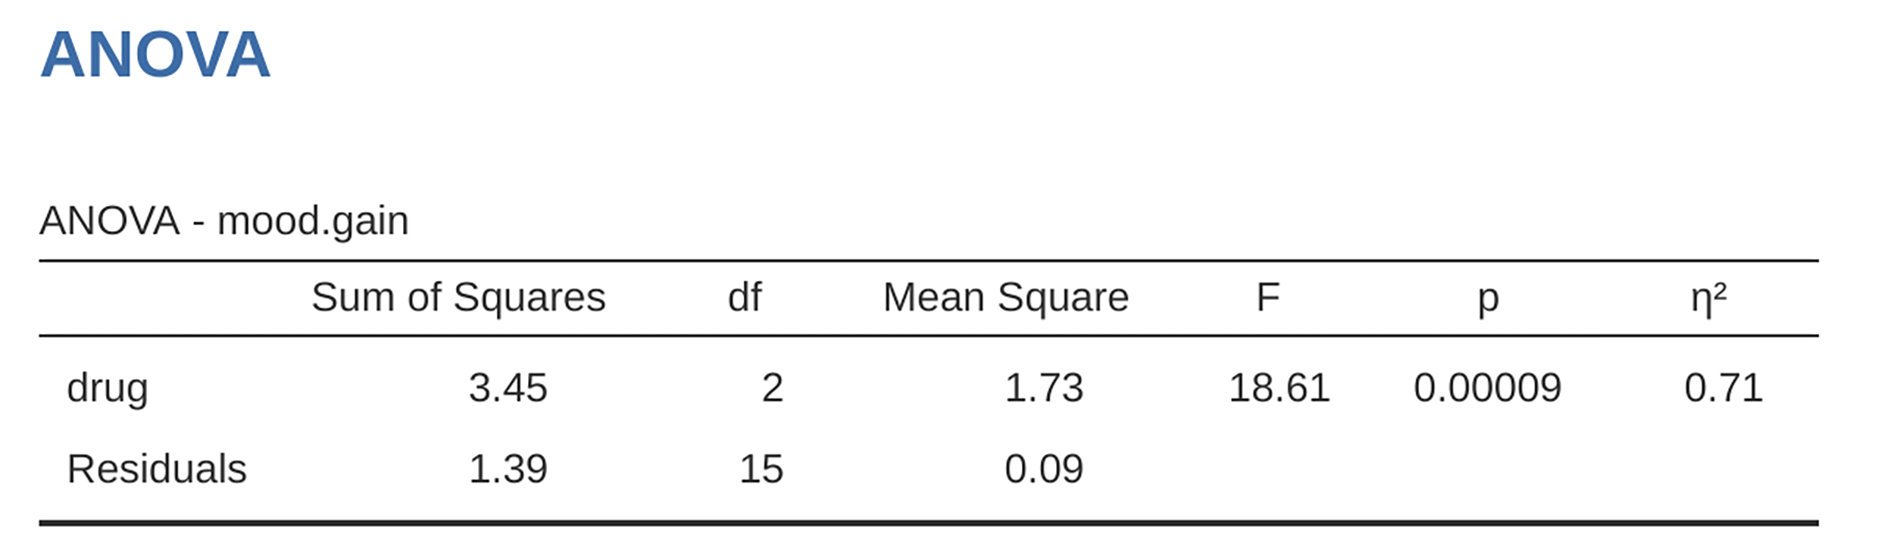
\includegraphics[width=1\textwidth,height=\textheight]{images/fig14-2.png} \hfill{}

\caption{\label{fig-fig14-2}jamovi one-way ANOVA of mood.gain by drug}

\end{figure}

Now, suppose I'm also curious to find out if therapy has a relationship
to mood.gain. In light of what we've seen from our discussion of
multiple regression in \textbf{?@sec-Correlation-and-linear-regression},
you probably won't be surprised that all we have to do is add therapy as
a second `Fixed Factor' in the analysis, see Figure~\ref{fig-fig14-3}.

\begin{figure}

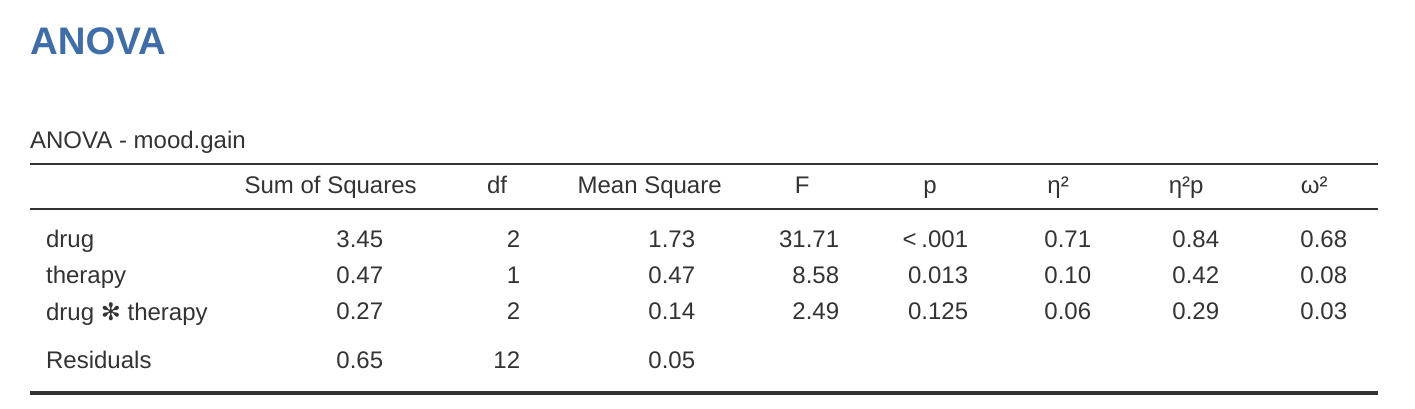
\includegraphics[width=1\textwidth,height=\textheight]{images/fig14-3.png} \hfill{}

\caption{\label{fig-fig14-3}jamovi two-way anova of mood.gain by drug
and therapy}

\end{figure}

This output is pretty simple to read too. The first row of the table
reports a between-group sum of squares (\(SS\)) value associated with
the drug factor, along with a corresponding between-group \(df\) value.
It also calculates a mean square value (\(MS\)), an \(F\)-statistic and
a \(p\)-value. There is also a row corresponding to the therapy factor,
a row corresponding to the interaction between the drug factor and the
therapy factor (which we won't cover just yet -- more on interactions
later), and a row corresponding to the residuals (i.e., the within
groups variation).

Not only are all of the individual quantities pretty familiar, the
relationships between these different quantities have remained
unchanged, just like we saw with the original one-way ANOVA. Note that
the mean square value is calculated by dividing \(SS\) by the
corresponding \(df\). That is, it's still true that:

\[MS=\frac{SS}{df}\]

regardless of whether we're talking about drug, therapy or the
residuals. To see this, let's not worry about how the sums of squares
values are calculated. Instead, let's take it on faith that jamovi has
calculated the \(SS\) values correctly, and try to verify that all the
rest of the numbers make sense. First, note that for the drug factor, we
divide \(3.45\) by \(2\) and end up with a mean square value of
\(1.73\). For the therapy factor, there's only 1 degree of freedom, so
our calculations are even simpler: dividing \(0.47\) (the \(SS\) value)
by 1 gives us an answer of \(0.47\) (the \(MS\) value).

Turning to the \(F\)-statistics and the \(p\)-values, notice that we
have one corresponding to the drug factor and one corresponding to the
therapy factor. Regardless of which one we're talking about, the
\(F\)-statistic is calculated by dividing the mean square value
associated with the factor by the mean square value associated with the
residuals. If we use ``A'' as shorthand notation to refer to the first
factor (Factor A; in this case drug) and ``R'' as shorthand notation to
refer to the residuals, then the \(F\)-statistic associated with Factor
A is denoted \(F_A\), and is calculated as follows:

\[F_A=\frac{MS_A}{MS_R}\]

and an equivalent formula exists for Factor B (i.e., therapy). Note that
this use of ``R'' to refer to residuals is a bit awkward, since we also
used the letter R to refer to the number of rows in the table, but I'm
only going to use ``R'' to mean residuals in the context of \({SS_R}\)
and \({MS_R}\), so hopefully this shouldn't be confusing. Anyway, to
apply this formula to the drugs factor we take the mean square of 1.73
and divide it by the residual mean square value of \(0.05\), which gives
us an \(F\)-statistic of 31.71.\footnote{NB There are some rounding
  errors here, the value of the mean square, to 5 decimal places, is
  1.72667. And the value of the residual mean square to 5 decimal
  places, is 0.05444. jamovi actually uses many more decimal places in
  its calculations, but the figures shown in the results tables are
  rounded for clarity. Though you can change the number of decimal
  places displayed by jamovi if you want.} The corresponding calculation
for the therapy variable would be to divide \(0.47\) by \(0.05\) which
gives \(8.58\) as the \(F\)-statistic. Not surprisingly, of course,
these are the same values that jamovi has reported in the ANOVA table
above.

Also in the ANOVA table is the calculation of the \(p\)-values. Once
again, there is nothing new here. For each of our two factors what we're
trying to do is test the null hypothesis that there is no relationship
between the factor and the outcome variable (I'll be a bit more precise
about this later on). To that end, we've (apparently) followed a similar
strategy to what we did in the one-way ANOVA and have calculated an
\(F\)-statistic for each of these hypotheses. To convert these to
\(p\)-values, all we need to do is note that the sampling distribution
for the \(F\)-statistic under the null hypothesis (that the factor in
question is irrelevant) is an \(F\)-distribution. Also note that the two
degrees of freedom values are those corresponding to the factor and
those corresponding to the residuals. For the drug factor we're talking
about an \(F\)-distribution with 2 and 12 degrees of freedom (I'll
discuss degrees of freedom in more detail later). In contrast, for the
therapy factor the sampling distribution is \(F\) with 1 and 12 degrees
of freedom.

At this point, I hope you can see that the ANOVA table for this more
complicated factorial analysis should be read in much the same way as
the ANOVA table for the simpler one way analysis. In short, it's telling
us that the factorial ANOVA for our \(3 \times 2\) design found a
significant effect of drug (\(F_{2,12} = 31.71, p < .001\)) as well as a
significant effect of therapy (\(F_{1,12} = 8.58, p = .013\)). Or, to
use the more technically correct terminology, we would say that there
are two \textbf{main effects} of drug and therapy. At the moment, it
probably seems a bit redundant to refer to these as ``main'' effects,
but it actually does make sense. Later on, we're going to cover
``interactions'' between the two factors, and so we generally make a
distinction between main effects and interaction effects.

\hypertarget{how-are-the-sum-of-squares-calculated}{%
\subsection{How are the sum of squares
calculated?}\label{how-are-the-sum-of-squares-calculated}}

In the previous section I had two goals. Firstly, to show you that the
jamovi method needed to do factorial ANOVA is pretty much the same as
what we used for a one-way ANOVA. The only difference is the addition of
a second factor. Secondly, I wanted to show you what the ANOVA table
looks like in this case, so that you can see from the outset that the
basic logic and structure behind factorial ANOVA is the same as that
which underpins one-way ANOVA. Try to hold onto that feeling. It's
genuinely true, insofar as factorial ANOVA is built in more or less the
same way as the simpler one-way ANOVA model. It's just that this feeling
of familiarity starts to evaporate once you start digging into the
details. Traditionally, this comforting sensation is replaced by an urge
to hurl abuse at the authors of statistics textbooks.

Okay, let's start by looking at some of those details. The explanation
that I gave in the last section illustrates the fact that the hypothesis
tests for the main effects (of drug and therapy in this case) are
\(F\)-tests, but what it doesn't do is show you how the sum of squares
(\(SS\)) values are calculated. Nor does it tell you explicitly how to
calculate degrees of freedom (\(df\) values) though that's a simple
thing by comparison. Let's assume for now that we have only two
predictor variables, Factor A and Factor B. If we use \(Y\) to refer to
the outcome variable, then we would use \(Y{rci}\) to refer to the
outcome associated with the \(i\)-th member of group \(rc\) (i.e.,
level/row \(r\) for Factor A and level/column \(c\) for Factor B). Thus,
if we use \(\bar{Y}\) to refer to a sample mean, we can use the same
notation as before to refer to group means, marginal means and grand
means. That is, \(\bar{Y}_{rc}\) is the sample mean associated with the
\(r\)th level of Factor A and the \(c\)th level of Factor B,
\(\bar{Y}_{r.}\) would be the marginal mean for the \(r\)th level of
Factor A, \(\bar{Y}_{.c}\) would be the marginal mean for the \(c\)th
level of Factor B, and \(\bar{Y}_{..}\) is the grand mean. In other
words, our sample means can be organised into the same table as the
population means. For our clinical trial data, that table is shown in
Table~\ref{tbl-tab14-5}.

\hypertarget{tbl-tab14-5}{}
 
  \providecommand{\huxb}[2]{\arrayrulecolor[RGB]{#1}\global\arrayrulewidth=#2pt}
  \providecommand{\huxvb}[2]{\color[RGB]{#1}\vrule width #2pt}
  \providecommand{\huxtpad}[1]{\rule{0pt}{#1}}
  \providecommand{\huxbpad}[1]{\rule[-#1]{0pt}{#1}}

\begin{table}[ht]
\caption{\label{tbl-tab14-5}Notation for sample means for the clinical trial data }\tabularnewline

\begin{centerbox}
\begin{threeparttable}
\setlength{\tabcolsep}{0pt}
\begin{tabularx}{0.9\textwidth}{p{0.225\textwidth} p{0.225\textwidth} p{0.225\textwidth} p{0.225\textwidth}}


\hhline{>{\huxb{0, 0, 0}{0.4}}->{\huxb{0, 0, 0}{0.4}}->{\huxb{0, 0, 0}{0.4}}->{\huxb{0, 0, 0}{0.4}}-}
\arrayrulecolor{black}

\multicolumn{1}{!{\huxvb{0, 0, 0}{0}}p{0.225\textwidth}!{\huxvb{0, 0, 0}{0}}}{\hspace{0pt}\parbox[b]{0.225\textwidth-0pt-12pt}{\huxtpad{2pt + 1em}\centering \textbf{}\huxbpad{2pt}}} &
\multicolumn{1}{p{0.225\textwidth}!{\huxvb{0, 0, 0}{0}}}{\hspace{12pt}\parbox[b]{0.225\textwidth-12pt-12pt}{\huxtpad{2pt + 1em}\centering \textbf{no therapy}\huxbpad{2pt}}} &
\multicolumn{1}{p{0.225\textwidth}!{\huxvb{0, 0, 0}{0}}}{\hspace{12pt}\parbox[b]{0.225\textwidth-12pt-12pt}{\huxtpad{2pt + 1em}\centering \textbf{CBT}\huxbpad{2pt}}} &
\multicolumn{1}{p{0.225\textwidth}!{\huxvb{0, 0, 0}{0}}}{\hspace{12pt}\parbox[b]{0.225\textwidth-12pt-0pt}{\huxtpad{2pt + 1em}\centering \textbf{total}\huxbpad{2pt}}} \tabularnewline[-0.5pt]


\hhline{>{\huxb{0, 0, 0}{0.4}}->{\huxb{0, 0, 0}{0.4}}->{\huxb{0, 0, 0}{0.4}}->{\huxb{0, 0, 0}{0.4}}-}
\arrayrulecolor{black}

\multicolumn{1}{!{\huxvb{0, 0, 0}{0}}p{0.225\textwidth}!{\huxvb{0, 0, 0}{0}}}{\hspace{0pt}\parbox[b]{0.225\textwidth-0pt-12pt}{\huxtpad{2pt + 1em}\centering placebo\huxbpad{2pt}}} &
\multicolumn{1}{p{0.225\textwidth}!{\huxvb{0, 0, 0}{0}}}{\hspace{12pt}\parbox[b]{0.225\textwidth-12pt-12pt}{\huxtpad{2pt + 1em}\centering \( \bar{Y}_{11} \)\huxbpad{2pt}}} &
\multicolumn{1}{p{0.225\textwidth}!{\huxvb{0, 0, 0}{0}}}{\hspace{12pt}\parbox[b]{0.225\textwidth-12pt-12pt}{\huxtpad{2pt + 1em}\centering \( \bar{Y}_{12} \)\huxbpad{2pt}}} &
\multicolumn{1}{p{0.225\textwidth}!{\huxvb{0, 0, 0}{0}}}{\hspace{12pt}\parbox[b]{0.225\textwidth-12pt-0pt}{\huxtpad{2pt + 1em}\centering \( \bar{Y}_{1.} \)\huxbpad{2pt}}} \tabularnewline[-0.5pt]


\hhline{}
\arrayrulecolor{black}

\multicolumn{1}{!{\huxvb{0, 0, 0}{0}}p{0.225\textwidth}!{\huxvb{0, 0, 0}{0}}}{\hspace{0pt}\parbox[b]{0.225\textwidth-0pt-12pt}{\huxtpad{2pt + 1em}\centering anxifree\huxbpad{2pt}}} &
\multicolumn{1}{p{0.225\textwidth}!{\huxvb{0, 0, 0}{0}}}{\hspace{12pt}\parbox[b]{0.225\textwidth-12pt-12pt}{\huxtpad{2pt + 1em}\centering \( \bar{Y}_{21} \)\huxbpad{2pt}}} &
\multicolumn{1}{p{0.225\textwidth}!{\huxvb{0, 0, 0}{0}}}{\hspace{12pt}\parbox[b]{0.225\textwidth-12pt-12pt}{\huxtpad{2pt + 1em}\centering \( \bar{Y}_{22} \)\huxbpad{2pt}}} &
\multicolumn{1}{p{0.225\textwidth}!{\huxvb{0, 0, 0}{0}}}{\hspace{12pt}\parbox[b]{0.225\textwidth-12pt-0pt}{\huxtpad{2pt + 1em}\centering \( \bar{Y}_{2.} \)\huxbpad{2pt}}} \tabularnewline[-0.5pt]


\hhline{}
\arrayrulecolor{black}

\multicolumn{1}{!{\huxvb{0, 0, 0}{0}}p{0.225\textwidth}!{\huxvb{0, 0, 0}{0}}}{\hspace{0pt}\parbox[b]{0.225\textwidth-0pt-12pt}{\huxtpad{2pt + 1em}\centering joyzepam\huxbpad{2pt}}} &
\multicolumn{1}{p{0.225\textwidth}!{\huxvb{0, 0, 0}{0}}}{\hspace{12pt}\parbox[b]{0.225\textwidth-12pt-12pt}{\huxtpad{2pt + 1em}\centering \( \bar{Y}_{31} \)\huxbpad{2pt}}} &
\multicolumn{1}{p{0.225\textwidth}!{\huxvb{0, 0, 0}{0}}}{\hspace{12pt}\parbox[b]{0.225\textwidth-12pt-12pt}{\huxtpad{2pt + 1em}\centering \( \bar{Y}_{32} \)\huxbpad{2pt}}} &
\multicolumn{1}{p{0.225\textwidth}!{\huxvb{0, 0, 0}{0}}}{\hspace{12pt}\parbox[b]{0.225\textwidth-12pt-0pt}{\huxtpad{2pt + 1em}\centering \( \bar{Y}_{3.} \)\huxbpad{2pt}}} \tabularnewline[-0.5pt]


\hhline{}
\arrayrulecolor{black}

\multicolumn{1}{!{\huxvb{0, 0, 0}{0}}p{0.225\textwidth}!{\huxvb{0, 0, 0}{0}}}{\hspace{0pt}\parbox[b]{0.225\textwidth-0pt-12pt}{\huxtpad{2pt + 1em}\centering total\huxbpad{2pt}}} &
\multicolumn{1}{p{0.225\textwidth}!{\huxvb{0, 0, 0}{0}}}{\hspace{12pt}\parbox[b]{0.225\textwidth-12pt-12pt}{\huxtpad{2pt + 1em}\centering \( \bar{Y}_{.1} \)\huxbpad{2pt}}} &
\multicolumn{1}{p{0.225\textwidth}!{\huxvb{0, 0, 0}{0}}}{\hspace{12pt}\parbox[b]{0.225\textwidth-12pt-12pt}{\huxtpad{2pt + 1em}\centering \( \bar{Y}_{.2} \)\huxbpad{2pt}}} &
\multicolumn{1}{p{0.225\textwidth}!{\huxvb{0, 0, 0}{0}}}{\hspace{12pt}\parbox[b]{0.225\textwidth-12pt-0pt}{\huxtpad{2pt + 1em}\centering \( \bar{Y}_{..} \)\huxbpad{2pt}}} \tabularnewline[-0.5pt]


\hhline{>{\huxb{0, 0, 0}{0.4}}->{\huxb{0, 0, 0}{0.4}}->{\huxb{0, 0, 0}{0.4}}->{\huxb{0, 0, 0}{0.4}}-}
\arrayrulecolor{black}
\end{tabularx} 

\end{threeparttable}\par\end{centerbox}

\end{table}
 

And if we look at the sample means that I showed earlier, we have
\(\bar{Y}_{11} = 0.30\), \(\bar{Y}_{12} = 0.60\) etc. In our clinical
trial example, the drugs factor has 3 levels and the therapy factor has
2 levels, and so what we're trying to run is a \(3 \times 2\) factorial
ANOVA. However, we'll be a little more general and say that Factor A
(the row factor) has \(r\) levels and Factor B (the column factor) has
\(c\) levels, and so what we're running here is an \(r \times c\)
factorial ANOVA.

{[}Additional technical detail\footnote{Now that we've got our notation
  straight, we can compute the sum of squares values for each of the two
  factors in a relatively familiar way. For Factor A, our between group
  sum of squares is calculated by assessing the extent to which the
  (row) marginal means \(\bar{Y}_{1.} , \bar{Y}_{2.}\) etc, are
  different from the grand mean \(\bar{Y}_{..}\) We do this in the same
  way that we did for one-way ANOVA: calculate the sum of squared
  difference between the \(\bar{Y}_{i.}\) values and the
  \(\bar{Y}_{..}\) values. Specifically, if there are \(N\) people in
  each group, then we calculate this:
  \[SS_A=(N \times C)\sum_{r=1}^R (\bar{Y}_{r.}-\bar{Y}_{..})^2\] As
  with one-way ANOVA, the most interesting\(^a\) part of this formula is
  the bit, which corresponds to the squared deviation associated with
  level \(r\). All that this formula does is calculate this squared
  deviation for all \(R\) levels of the factor, add them up, and then
  multiply the result by \(N \times C\). The reason for this last part
  is that there are multiple cells in our design that have level \(r\)
  on Factor A. In fact, there are \(C\) of them, one corresponding to
  each possible level of Factor B. For instance, in our example there
  are two different cells in the design corresponding to the anxifree
  drug: one for people with no.therapy and one for the CBT group. Not
  only that, within each of these cells there are \(N\) observations.
  So, if we want to convert our \(SS\) value into a quantity that
  calculates the between groups sum of squares on a ``per observation''
  basis, we have to multiply by \(N \times C\). The formula for Factor B
  is of course the same thing, just with some subscripts shuffled around
  \[SS_B=(N \times R)\sum_{c=1}^C (\bar{Y}_{.c}-\bar{Y}_{..})^2\] Now
  that we have these formulas we can check them against the jamovi
  output from the earlier section. Once again, a dedicated spreadsheet
  programme is helpful for these sorts of calculations, so please have a
  go yourself. You can also take a look at the version I did in Excel in
  the file \emph{clinicaltrial\_factorialanova.xls}. First, let's
  calculate the sum of squares associated with the main effect of drug.
  There are a total of \(N = 3\) people in each group and \(C = 2\)
  different types of therapy. Or, to put it another way, there are
  \(3 \times 2 = 6\) people who received any particular drug. When we do
  these calculations in a spreadsheet programme, we get a value of 3.45
  for the sum of squares associated with the main effect of drug. Not
  surprisingly, this is the same number that you get when you look up
  the \(SS\) value for the drugs factor in the ANOVA table that I
  presented earlier, in Figure~\ref{fig-fig14-3}. We can repeat the same
  kind of calculation for the effect of therapy. Again there are
  \(N = 3\) people in each group, but since there are \(R = 3\)
  different drugs, this time around we note that there are
  \(3 \times 3 = 9\) people who received CBT and an additional 9 people
  who received the placebo. So our calculation in this case gives us a
  value of \(0.47\) for the sum of squares associated with the main
  effect of therapy. Once again, we are not surprised to see that our
  calculations are identical to the ANOVA output in
  Figure~\ref{fig-fig14-3}. So that's how you calculate the \(SS\)
  values for the two main effects. These \(SS\) values are analogous to
  the between group sum of squares values that we calculated when doing
  one-way ANOVA in \textbf{?@sec-Comparing-several-means-one-way-ANOVA}.
  However, it's not a good idea to think of them as between groups
  \(SS\) values anymore, just because we have two different grouping
  variables and it's easy to get confused. In order to construct an
  \(F\) test, however, we also need to calculate the within groups sum
  of squares. In keeping with the terminology that we used in
  \textbf{?@sec-Correlation-and-linear-regression} and the terminology
  that jamovi uses when printing out the ANOVA table, I'll start
  referring to the within groups \(SS\) value as the residual sum of
  squares \(SS_R\). The easiest way to think about the residual \(SS\)
  values in this context, I think, is to think of it as the leftover
  variation in the outcome variable after you take into account the
  differences in the marginal means (i.e., after you remove \(SS_A\) and
  \(SS_B\)). What I mean by that is we can start by calculating the
  total sum of squares, which I'll label \(SS_T\) . The formula for this
  is pretty much the same as it was for one-way ANOVA. We take the
  difference between each observation \(Y_{rci}\) and the grand mean
  \(\hat{Y}_{..}\), square the differences, and add them all
  \[SS_T=\sum_{r=1}^R \sum_{c=1}^C \sum_{i=1}^N (Y_{rci}-\bar{Y}_{..})^2\]
  The ``triple summation'' here looks more complicated than it is. In
  the first two summations, we're summing across all levels of Factor A
  (i.e., over all possible rows r in our table) and across all levels of
  Factor B (i.e., all possible columns \(c\)). Each rc combination
  corresponds to a single group and each group contains \(N\) people, so
  we have to sum across all those people (i.e., all \(i\) values) too.
  In other words, all we're doing here is summing across all
  observations in the data set (i.e., all possible \(rci\)
  combinations). At this point, we know the total variability of the
  outcome variable \(SST\) , and we know how much of that variability
  can be attributed to Factor A (\(SS_A\)) and how much of it can be
  attributed to Factor B (\(SS_B\)). The residual sum of squares is thus
  defined to be the variability in \(Y\) that can't be attributed to
  either of our two factors (or their interaction if you also calculate
  the interaction effect, which is the default in jamovi). In other
  words \[SS_R=SS_T-(SS_A+SS_B)\] Of course, there is a formula that you
  can use to calculate the residual \(SS\) directly, but I think that it
  makes more conceptual sense to think of it like this. The whole point
  of calling it a residual is that it's the leftover variation, and the
  formula above makes that clear. I should also note that, in keeping
  with the terminology used in the regression chapter, it is commonplace
  to refer to \(SS_A + SS_B\) as the variance attributable to the
  ``ANOVA model'', denoted \(SSM\), and so we often say that the total
  sum of squares is equal to the model sum of squares plus the residual
  sum of squares. Later on in this chapter we'll see that this isn't
  just a surface similarity: ANOVA and regression are actually the same
  thing under the hood. In any case, it's probably worth taking a moment
  to check that we can calculate \(SS_R\) using this formula and verify
  that we do obtain the same answer that jamovi produces in its ANOVA
  table. The calculations are pretty straightforward when done in a
  spreadsheet (see the clinicaltrial\_factorialanova.xls file). ---
  \(^a\)English translation: ``least tedious''.}{]}

\hypertarget{what-are-our-degrees-of-freedom}{%
\subsection{What are our degrees of
freedom?}\label{what-are-our-degrees-of-freedom}}

The degrees of freedom are calculated in much the same way as for
one-way ANOVA. For any given factor, the degrees of freedom is equal to
the number of levels minus 1 (i.e., \(R - 1\) for the row variable
Factor A, and \(C - 1\) for the column variable Factor B). So, for the
drugs factor we obtain \(df = 2\), and for the therapy factor we obtain
\(df = 1\). Later on, when we discuss the interpretation of ANOVA as a
regression model (see Section~\ref{sec-ANOVA-as-a-linear-model}), I'll
give a clearer statement of how we arrive at this number. But for the
moment we can use the simple definition of degrees of freedom, namely
that the degrees of freedom equals the number of quantities that are
observed, minus the number of constraints. So, for the drugs factor, we
observe 3 separate group means, but these are constrained by 1 grand
mean, and therefore the degrees of freedom is 2.

\hypertarget{factorial-anova-versus-one-way-anovas}{%
\subsection{Factorial ANOVA versus one-way
ANOVAs}\label{factorial-anova-versus-one-way-anovas}}

Now that we've seen how a factorial ANOVA works, it's worth taking a
moment to compare it to the results of the one way analyses, because
this will give us a really good sense of why it's a good idea to run the
factorial ANOVA. In \textbf{?@sec-Comparing-several-means-one-way-ANOVA}
I ran a one-way ANOVA that looked to see if there are any differences
between drugs, and a second one-way ANOVA to see if there were any
differences between therapies. As we saw in the section
Section~\ref{sec-What-hypotheses-are-we-testing}, the null and
alternative hypotheses tested by the one-way ANOVAs are in fact
identical to the hypotheses tested by the factorial ANOVA. Looking even
more carefully at the ANOVA tables, we can see that the sum of squares
associated with the factors are identical in the two different analyses
(3.45 for drug and 0.92 for therapy), as are the degrees of freedom (2
for drug, 1 for therapy). But they don't give the same answers! Most
notably, when we ran the one-way ANOVA for therapy in
\textbf{?@sec-On-the-relationship-between-ANOVA-and-the-Student-t-test}
we didn't find a significant effect (the \(p\)-value was .21). However,
when we look at the main effect of therapy within the context of the
two-way ANOVA, we do get a significant effect (\(p\) = .019). The two
analyses are clearly not the same.

Why does that happen? The answer lies in understanding how the residuals
are calculated. Recall that the whole idea behind an \(F\)-test is to
compare the variability that can be attributed to a particular factor
with the variability that cannot be accounted for (the residuals). If
you run a one-way ANOVA for therapy, and therefore ignore the effect of
drug, the ANOVA will end up dumping all of the drug-induced variability
into the residuals! This has the effect of making the data look more
noisy than they really are, and the effect of therapy which is correctly
found to be significant in the two-way ANOVA now becomes
non-significant. If we ignore something that actually matters (e.g.,
drug) when trying to assess the contribution of something else (e.g.,
therapy) then our analysis will be distorted. Of course, it's perfectly
okay to ignore variables that are genuinely irrelevant to the phenomenon
of interest. If we had recorded the colour of the walls, and that turned
out to be a non-significant factor in a three-way ANOVA, it would be
perfectly okay to disregard it and just report the simpler two-way ANOVA
that doesn't include this irrelevant factor. What you shouldn't do is
drop variables that actually make a difference!

\hypertarget{what-kinds-of-outcomes-does-this-analysis-capture}{%
\subsection{What kinds of outcomes does this analysis
capture?}\label{what-kinds-of-outcomes-does-this-analysis-capture}}

The ANOVA model that we've been talking about so far covers a range of
different patterns that we might observe in our data. For instance, in a
two-way ANOVA design there are four possibilities: (a) only Factor A
matters, (b) only Factor B matters, (c) both A and B matter, and (d)
neither A nor B matters. An example of each of these four possibilities
is plotted in Figure~\ref{fig-fig14-4}.

\hypertarget{factorial-anova-2-balanced-designs-interpreting-interactions}{%
\section{Factorial ANOVA 2: balanced designs, interpreting
interactions}\label{factorial-anova-2-balanced-designs-interpreting-interactions}}

The four patterns of data shown in Figure~\ref{fig-fig14-4} are all
quite realistic. There are a great many data sets that produce exactly
those patterns. However, they are not the whole story and the ANOVA
model that we have been talking about up to this point is not sufficient
to fully account for a table of group means. Why not? Well, so far we
have the ability to talk about the idea that drugs can influence mood,
and therapy can influence mood, but no way of talking about the
possibility of an \textbf{interaction} between the two. An interaction
between A and B is said to occur whenever the effect of Factor \(A\) is
\emph{different}, depending on which level of Factor \(B\) we're talking
about. Several examples of an interaction effect with the context of a
\(2 \times 2\) ANOVA are shown in Figure~\ref{fig-fig14-5}. To give a
more concrete example, suppose that the operation of Anxifree and
Joyzepam is governed by quite different physiological mechanisms. One
consequence of this is that while Joyzepam has more or less the same
effect on mood regardless of whether one is in therapy, Anxifree is
actually much more effective when administered in conjunction with CBT.
The ANOVA that we developed in the previous section does not capture
this idea. To get some idea of whether an interaction is actually
happening here, it helps to plot the various group means. In jamovi this
is done via the ANOVA `Estimated Marginal Means' option -- just move
drug and therapy across into the `Marginal Means' box under `Term 1'.
This should look something like Figure~\ref{fig-fig14-6}. Our main
concern relates to the fact that the two lines aren't parallel. The
effect of CBT (difference between solid line and dotted line) when the
drug is Joyzepam (right side) appears to be near zero, even smaller than
the effect of CBT when a placebo is used (left side). However, when
Anxifree is administered, the effect of CBT is larger than the placebo
(middle). Is this effect real, or is this just random variation due to
chance? Our original ANOVA cannot answer this question, because we make
no allowances for the idea that interactions even exist! In this
section, we'll fix this problem.

\begin{figure}

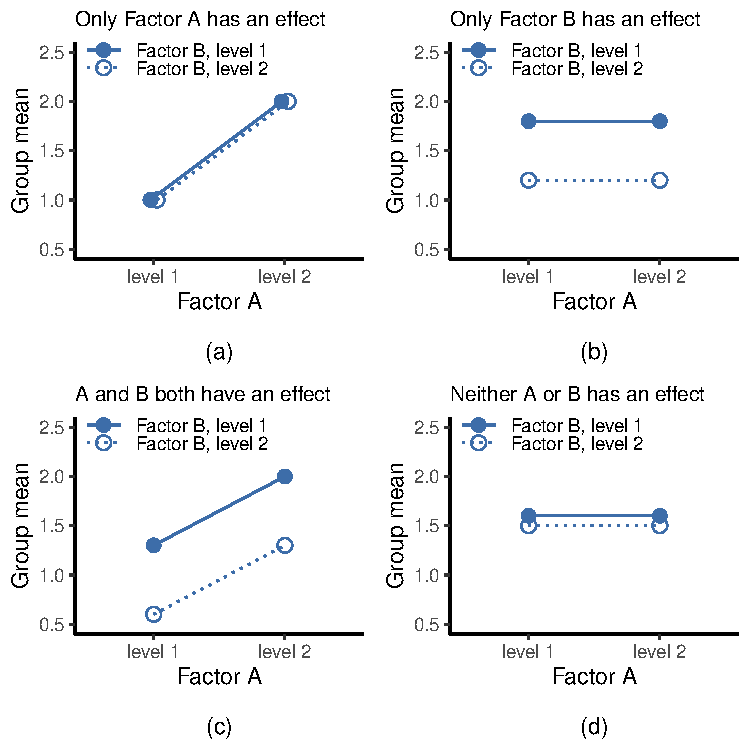
\includegraphics[width=1\textwidth,height=\textheight]{14-Factorial-ANOVA_files/figure-pdf/fig-fig14-4-1.pdf} \hfill{}

\caption{\label{fig-fig14-4}The four different outcomes for a
\(2 \times 2\) ANOVA when no interactions are present. In panel (a) we
see a main effect of Factor A and no effect of Factor B. Panel (b) shows
a main effect of Factor B but no effect of Factor A. Panel (c) shows
main effects of both Factor A and Factor B. Finally, panel (d) shows no
effect of either factor}

\end{figure}

\begin{figure}

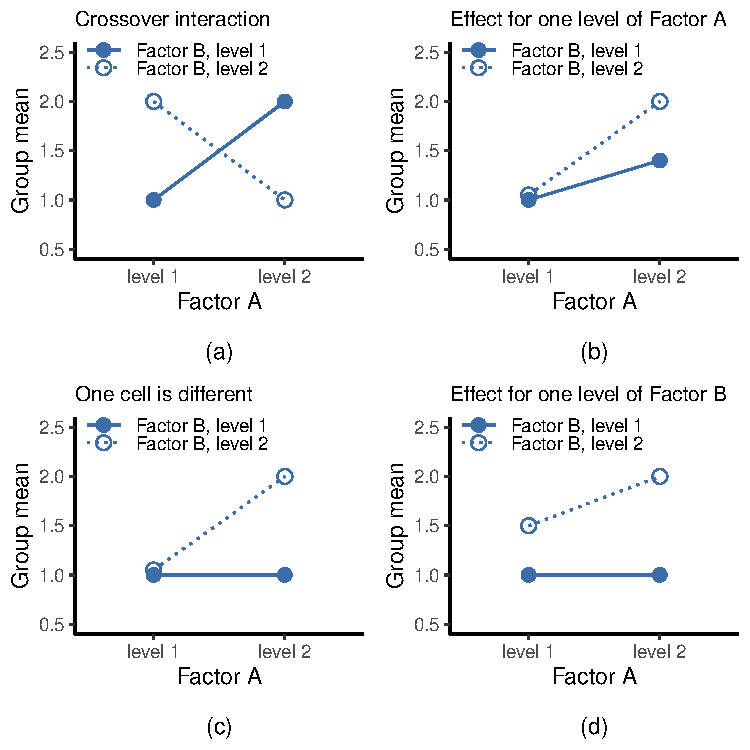
\includegraphics[width=1\textwidth,height=\textheight]{14-Factorial-ANOVA_files/figure-pdf/fig-fig14-5-1.pdf} \hfill{}

\caption{\label{fig-fig14-5}Qualitatively different interactions for a
\(2 \times 2\) ANOVA}

\end{figure}

\begin{figure}

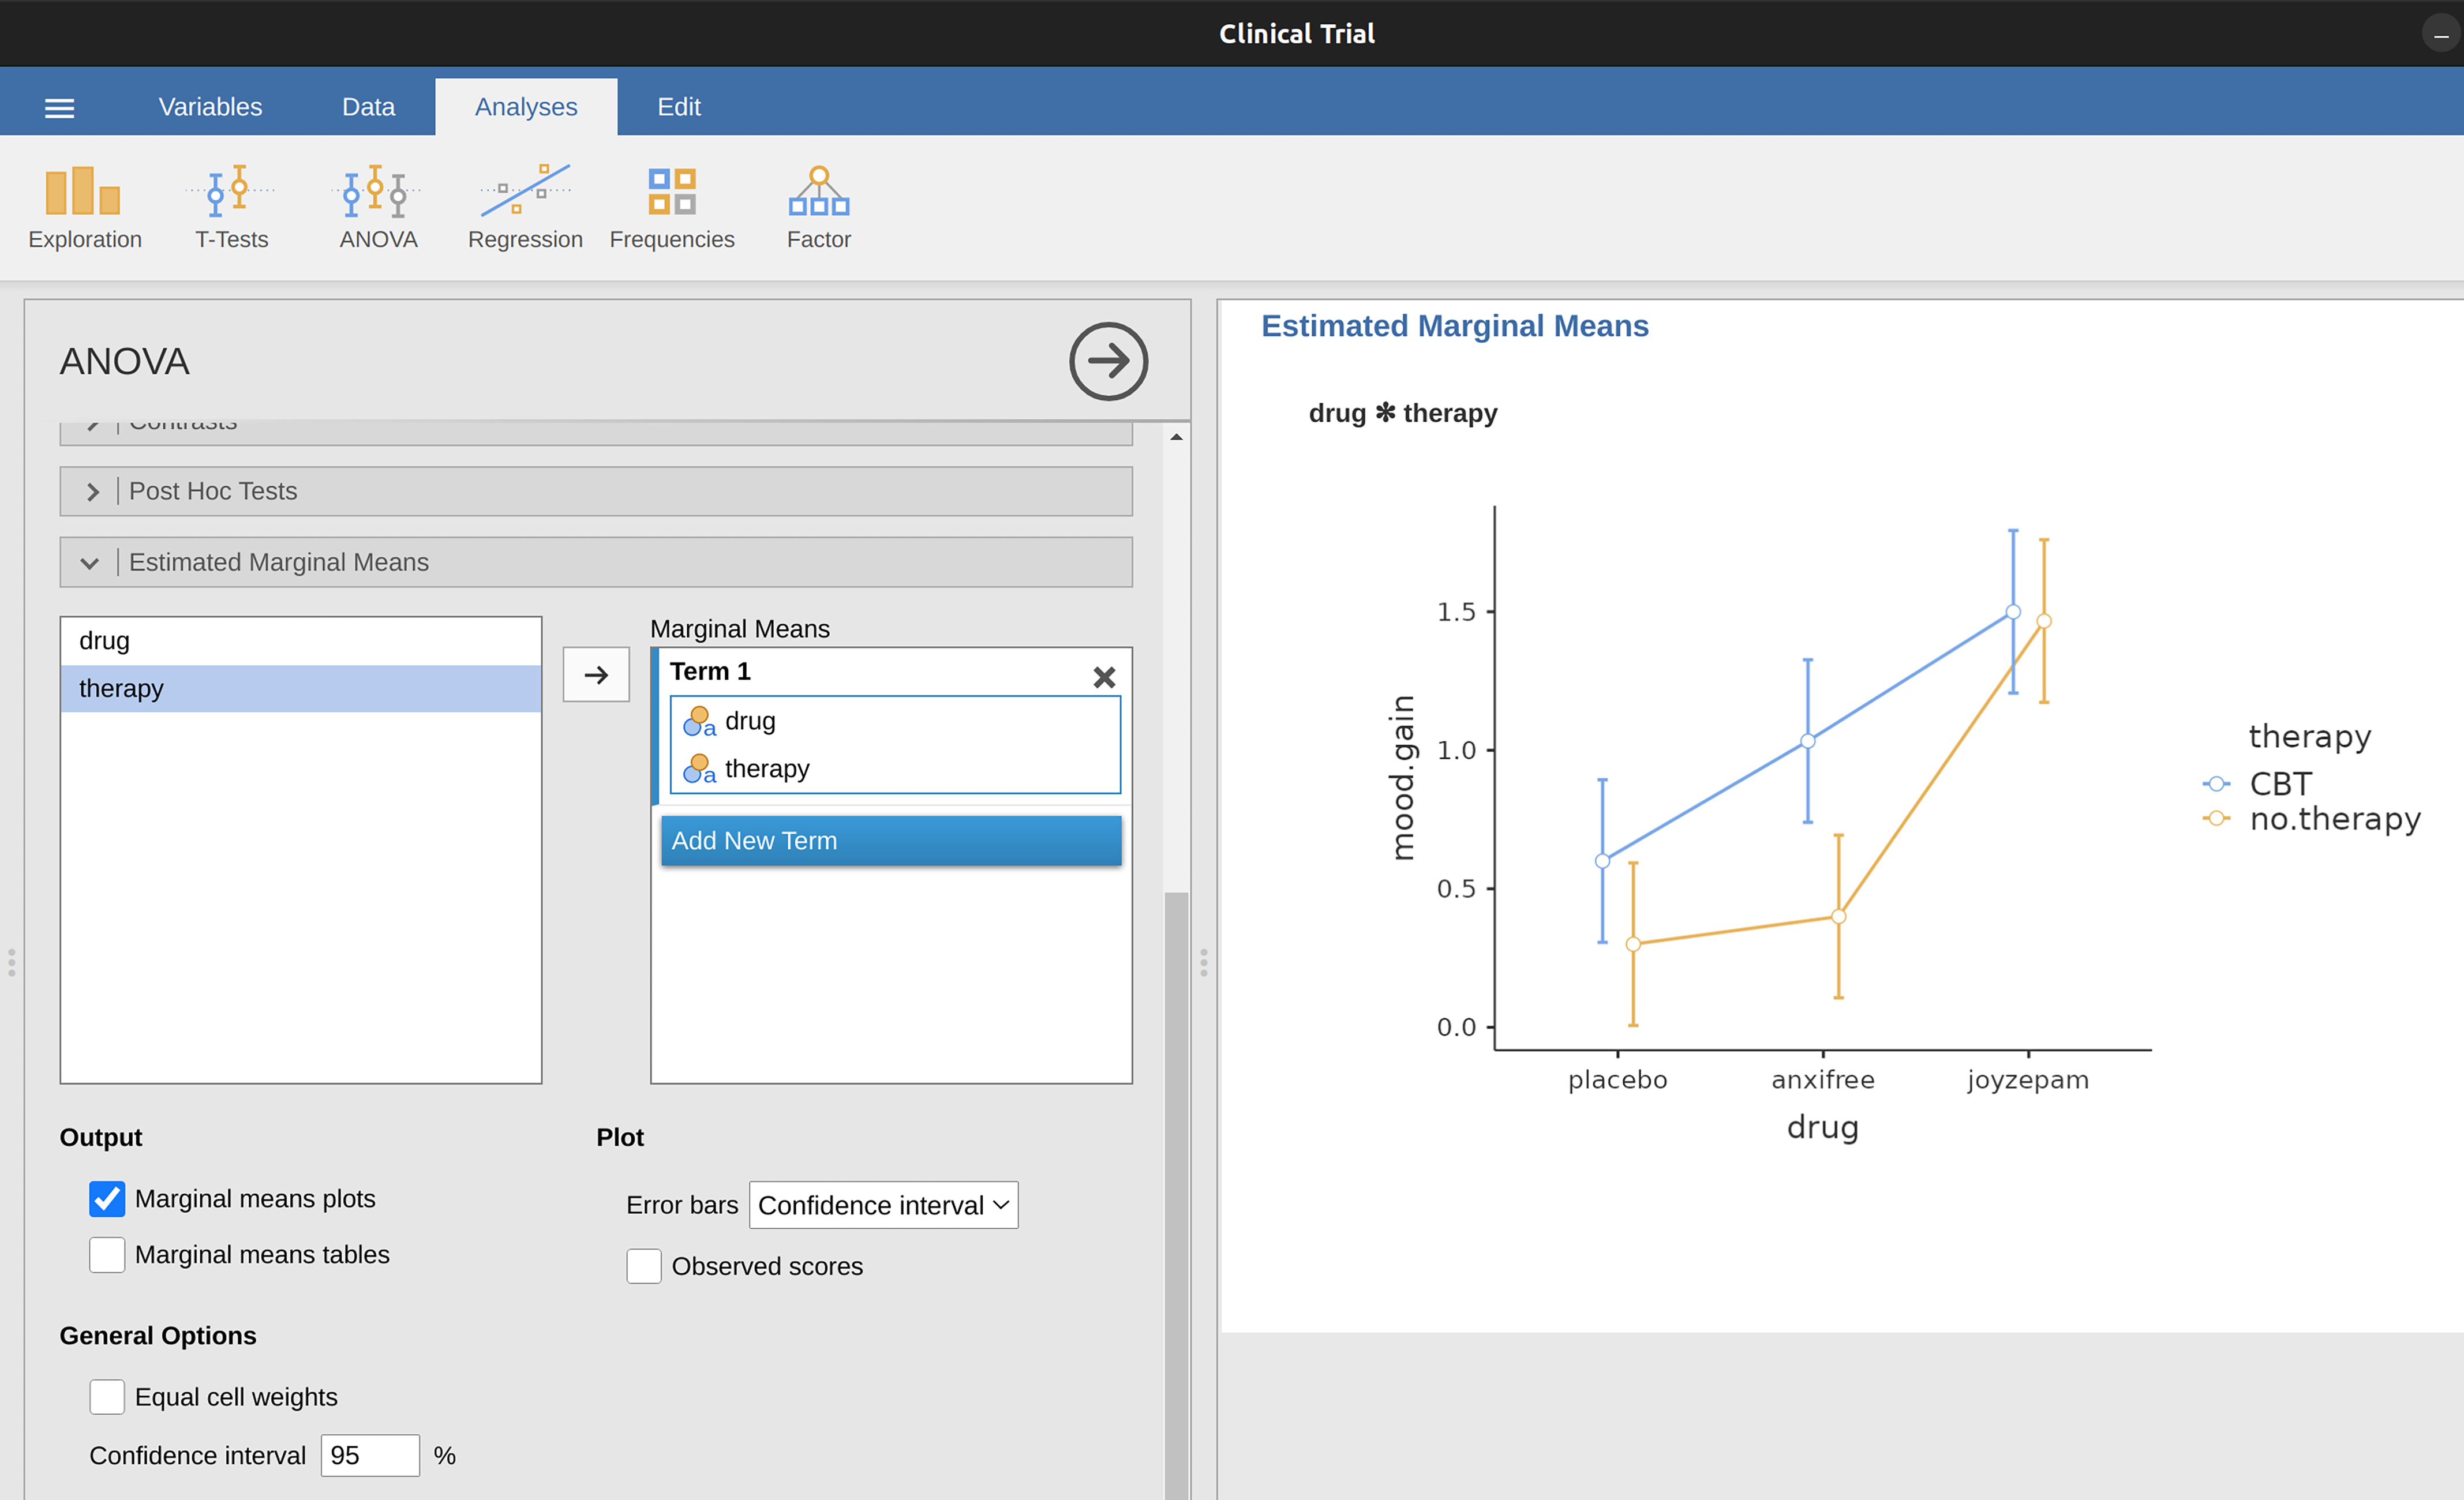
\includegraphics[width=1\textwidth,height=\textheight]{images/fig14-6.png} \hfill{}

\caption{\label{fig-fig14-6}jamovi screen showing how to generate a
descriptive interaction plot in ANOVA using the clinical trial data}

\end{figure}

\hypertarget{what-exactly-is-an-interaction-effect}{%
\subsection{What exactly is an interaction
effect?}\label{what-exactly-is-an-interaction-effect}}

The key idea that we're going to introduce in this section is that of an
interaction effect. In the ANOVA model we have looked at so far there
are only two factors involved in our model (i.e., drug and therapy). But
when we add an interaction we add a new component to the model: the
combination of drug and therapy. Intuitively, the idea behind an
interaction effect is fairly simple. It just means that the effect of
Factor A is different, depending on which level of Factor B we're
talking about. But what does that actually mean in terms of our data?
The plot in Figure~\ref{fig-fig14-5} depicts several different patterns
that, although quite different to each other, would all count as an
interaction effect. So it's not entirely straightforward to translate
this qualitative idea into something mathematical that a statistician
can work with.

{[}Additional technical detail\footnote{As a consequence, the way that
  the idea of an interaction effect is formalised in terms of null and
  alternative hypotheses is slightly difficult, and I'm guessing that a
  lot of readers of this book probably won't be all that interested.
  Even so, I'll try to give the basic idea here. To start with, we need
  to be a little more explicit about our main effects. Consider the main
  effect of Factor A (drug in our running example). We originally
  formulated this in terms of the null hypothesis that the two marginal
  means \(\mu_r\). are all equal to each other. Obviously, if all of
  these are equal to each other, then they must also be equal to the
  grand mean \(\mu_{..}\) as well, right? So what we can do is define
  the effect of Factor A at level \(r\) to be equal to the difference
  between the marginal mean \(\mu_{r.}\) and the grand mean
  \(\mu_{..}\). Let's denote this effect by \(\alpha_r\), and note that
  \[\alpha_r=\mu_{r.}-\mu_{..}\] Now, by definition all of the
  \(\alpha_r\) values must sum to zero, for the same reason that the
  average of the marginal means \(\mu_c\) must be the grand mean
  \(\mu_{..}\). We can similarly define the effect of Factor B at level
  \(i\) to be the difference between the column marginal mean
  \(\mu_{.c}\) and the grand mean \(\mu_{..}\)
  \[\beta_c=\mu_{.c}-\mu_{..}\] and once again, these \(\beta_c\) values
  must sum to zero. The reason that statisticians sometimes like to talk
  about the main effects in terms of these \(\alpha_r\) and \(\beta_c\)
  values is that it allows them to be precise about what it means to say
  that there is no interaction effect. If there is no interaction at
  all, then these \(\alpha_r\) and \(\beta_c\) values will perfectly
  describe the group means \(\mu_{rc}\). Specifically, it means that
  \[\mu_{rc}=\mu_{..}+\alpha_{r}+\beta_{c}\] That is, there's nothing
  special about the group means that you couldn't predict perfectly by
  knowing all the marginal means. And that's our null hypothesis, right
  there. The alternative hypothesis is that
  \[\mu_{rc} \neq \mu_{..}+\alpha_{r}+\beta_{c}\] for at least one group
  \(rc\) in our table. However, statisticians often like to write this
  slightly differently. They'll usually define the specific interaction
  associated with group \(rc\) to be some number, awkwardly referred to
  as \((\alpha \beta)_{rc}\), and then they will say that the
  alternative hypothesis is that
  \[\mu_{rc}=\mu_{..} +\alpha_{r} +\beta_{c} + (\alpha \beta )_{rc}\]
  where \((\alpha \beta)_{rc}\) is non-zero for at least one group. This
  notation is kind of ugly to look at, but it is handy as we'll see when
  discussing how to calculate the sum of squares. How should we
  calculate the sum of squares for the interaction terms, \(SS_{A:B}\)?
  Well, first off, it helps to notice how we have just defined the
  interaction effect in terms of the extent to which the actual group
  means differ from what you'd expect by just looking at the marginal
  means. Of course, all of those formulas refer to population parameters
  rather than sample statistics, so we don't actually know what they
  are. However, we can estimate them by using sample means in place of
  population means. So for Factor A, a good way to estimate the main
  effect at level \(r\) is as the difference between the sample marginal
  mean \(\bar{Y}_{rc}\) and the sample grand mean \(\bar{Y}_{..}\). That
  is, we would use this as our estimate of the effect
  \[\hat{\alpha}_r = bar{Y}_{r.}-\bar{Y}_{..}\] Similarly, our estimate
  of the main effect of Factor B at level \(c\) can be defined as
  follows \[\hat{\beta}_{c}=\hat{Y}_{.c}-\bar{Y}_{..}\] Now, if you go
  back to the formulas that I used to describe the \(SS\) values for the
  two main effects, you'll notice that these effect terms are exactly
  the quantities that we were squaring and summing! So, what's the
  analog of this for interaction terms? The answer to this can be found
  by first rearranging the formula for the group means \(\mu_{rc}\)
  under the alternative hypothesis, so that we get this
  \[\begin{aligned} (\alpha \beta)_{rc} & = \mu_{rc} - \mu_{..} - \alpha_r - \beta_c \\ & = \mu_{rc} - \mu_{..} - (\mu_{r.}-\mu_{..})-(\mu_{.c}-\mu_{..}) \\ & = \mu_{rc} - \mu_{r.} - \mu_{.c} +\mu_{..} \end{aligned}\]
  So, once again if we substitute our sample statistics in place of the
  population means, we get the following as our estimate of the
  interaction effect for group \(rc\), which is
  \[(\hat{\alpha \beta})_{rc}=\bar{Y}_{rc}-\hat{Y}_{r.}-\bar{Y}_{.c}+\bar{Y}_{..}\]
  Now all we have to do is sum all of these estimates across all \(R\)
  levels of Factor A and all \(C\) levels of Factor B, and we obtain the
  following formula for the sum of squares associated with the
  interaction as a whole
  \[SS_{A:B}=N \sum_{r=1}^R \sum_{c=1}^C (\bar{Y}_{rc}-\bar{Y}_{r.}-\bar{Y}_{.c}+\bar{Y}_{..})^2\]
  where we multiply by \(N\) because there are \(N\) observations in
  each of the groups, and we want our \(SS\) values to reflect the
  variation among observations accounted for by the interaction, not the
  variation among groups. Now that we have a formula for calculating
  \(SS_{A:B}\), it's important to recognise that the interaction term is
  part of the model (of course), so the total sum of squares associated
  with the model, \(SSM\), is now equal to the sum of the three relevant
  \(SS\) values, \(SS_A + SS_B + SS_{A:B}\). The residual sum of squares
  \(SSR\) is still defined as the leftover variation, namely
  \(SS_T - SS_M\), but now that we have the interaction term this
  becomes \[SS_R=SS_T-(SS_A+SS_B+SS_{A:B})\] As a consequence, the
  residual sum of squares \(SS_R\) will be smaller than in our original
  ANOVA that didn't include interactions.}{]}

\hypertarget{degrees-of-freedom-for-the-interaction}{%
\subsection{Degrees of freedom for the
interaction}\label{degrees-of-freedom-for-the-interaction}}

Calculating the degrees of freedom for the interaction is, once again,
slightly trickier than the corresponding calculation for the main
effects. To start with, let's think about the ANOVA model as a whole.
Once we include interaction effects in the model we're allowing every
single group to have a unique mean, \(mu_{rc}\). For an \(R \times C\)
factorial ANOVA, this means that there are \(R \times C\) quantities of
interest in the model and only the one constraint: all of the group
means need to average out to the grand mean. So the model as a whole
needs to have (\(R \times C)-1\) degrees of freedom. But the main effect
of Factor A has \(R-1\) degrees of freedom, and the main effect of
Factor B has \(C-1\) degrees of freedom. This means that the degrees of
freedom associated with the interaction is:

\[
\begin{aligned}
df_{A:B} & = (R \times C - 1) - (R - 1) - (C - 1) \\
& = RC - R - C + 1 \\
& = (R-1)(C-1)
\end{aligned}
\]

which is just the product of the degrees of freedom associated with the
row factor and the column factor.

What about the residual degrees of freedom? Because we've added
interaction terms which absorb some degrees of freedom, there are fewer
residual degrees of freedom left over. Specifically, note that if the
model with interaction has a total of \((R \times C) - 1\), and there
are \(N\) observations in your data set that are constrained to satisfy
1 grand mean, your residual degrees of freedom now become
\(N - (R \times C) - 1 + 1\), or just \(N - (R \times C)\).

\hypertarget{running-the-anova-in-jamovi}{%
\subsection{Running the ANOVA in
jamovi}\label{running-the-anova-in-jamovi}}

Adding interaction terms to the ANOVA model in jamovi is
straightforward. In fact it is more than straightforward because it is
the default option for ANOVA. This means that when you specify an ANOVA
with two factors, e.g.~drug and therapy then the interaction component
-- drug \(\times\) therapy -- is added automatically to the
model.\footnote{You may have spotted this already when looking at the
  main effects analysis in jamovi that we described earlier. For the
  purpose of the explanation in this book I removed the interaction
  component from the earlier model to keep things clean and simple.}
When we run the ANOVA with the interaction term included, then we get
the results shown in Figure~\ref{fig-fig14-7}.

\begin{figure}

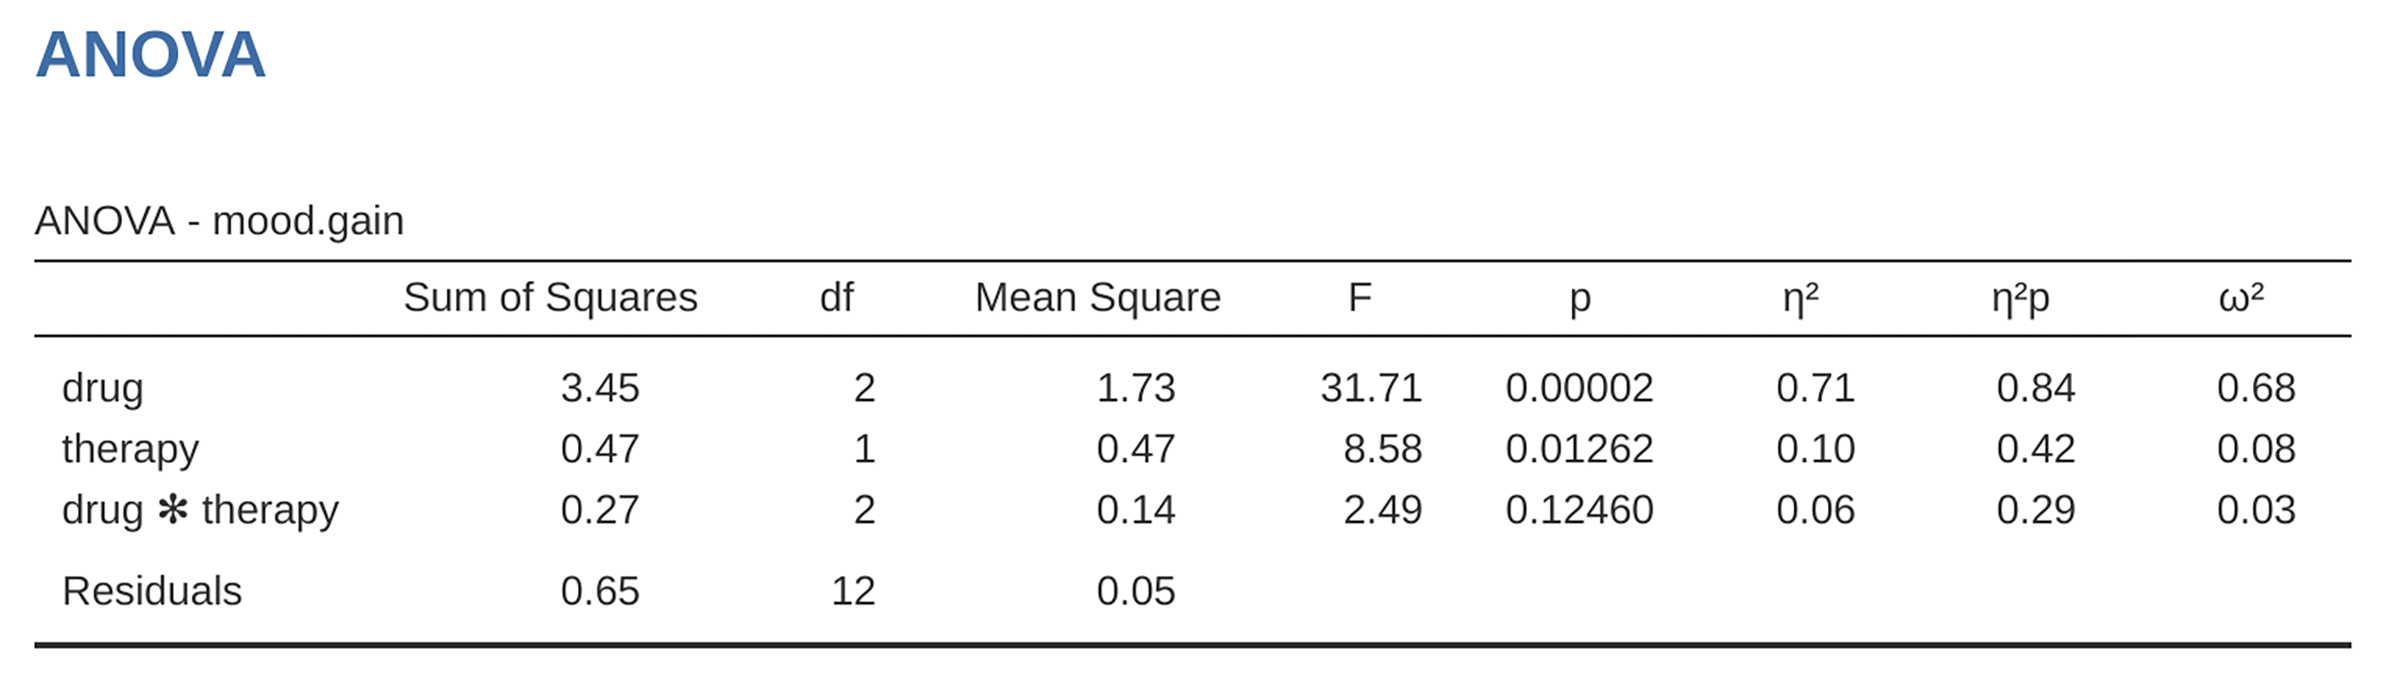
\includegraphics[width=1\textwidth,height=\textheight]{images/fig14-7.png} \hfill{}

\caption{\label{fig-fig14-7}Results for the full factorial model,
including the interaction component drug \(\times\) therapy}

\end{figure}

As it turns out, while we do have a significant main effect of drug
(\(F_{2,12} = 31.7, p < .001\)) and therapy type
(\(F_{1,12} = 8.6, p = .013\)), there is no significant interaction
between the two (\(F_{2,12} = 2.5, p = 0.125\)).

\hypertarget{interpreting-the-results}{%
\subsection{Interpreting the results}\label{interpreting-the-results}}

There's a couple of very important things to consider when interpreting
the results of factorial ANOVA. First, there's the same issue that we
had with one-way ANOVA, which is that if you obtain a significant main
effect of (say) drug, it doesn't tell you anything about which drugs are
different to one another. To find that out, you need to run additional
analyses. We'll talk about some analyses that you can run in later
Sections:
\protect\hyperlink{different-ways-to-specify-contrasts}{Different ways
to specify contrasts} and \protect\hyperlink{sec-Post-hoc-tests}{Post
hoc tests}. The same is true for interaction effects. Knowing that
there's a significant interaction doesn't tell you anything about what
kind of interaction exists. Again, you'll need to run additional
analyses.

Secondly, there's a very peculiar interpretation issue that arises when
you obtain a significant interaction effect but no corresponding main
effect. This happens sometimes. For instance, in the crossover
interaction shown in Figure~\ref{fig-fig14-5}(a), this is exactly what
you'd find. In this case, neither of the main effects would be
significant, but the interaction effect would be. This is a difficult
situation to interpret, and people often get a bit confused about it.
The general advice that statisticians like to give in this situation is
that you shouldn't pay much attention to the main effects when an
interaction is present. The reason they say this is that, although the
tests of the main effects are perfectly valid from a mathematical point
of view, when there is a significant interaction effect the main effects
rarely test interesting hypotheses. Recall from
Section~\ref{sec-What-hypotheses-are-we-testing} that the null
hypothesis for a main effect is that the marginal means are equal to
each other, and that a marginal mean is formed by averaging across
several different groups. But if you have a significant interaction
effect then you know that the groups that comprise the marginal mean
aren't homogeneous, so it's not really obvious why you would even care
about those marginal means.

Here's what I mean. Again, let's stick with a clinical example. Suppose
that we had a \(2 \times 2\) design comparing two different treatments
for phobias (e.g., systematic desensitisation vs flooding), and two
different anxiety reducing drugs (e.g., Anxifree vs Joyzepam). Now,
suppose what we found was that Anxifree had no effect when
desensitisation was the treatment, and Joyzepam had no effect when
flooding was the treatment. But both were pretty effective for the other
treatment. This is a classic crossover interaction, and what we'd find
when running the ANOVA is that there is no main effect of drug, but a
significant interaction. Now, what does it actually mean to say that
there's no main effect? Well, it means that if we average over the two
different psychological treatments, then the average effect of Anxifree
and Joyzepam is the same. But why would anyone care about that? When
treating someone for phobias it is never the case that a person can be
treated using an ``average'' of flooding and desensitisation. That
doesn't make a lot of sense. You either get one or the other. For one
treatment one drug is effective, and for the other treatment the other
drug is effective. The interaction is the important thing and the main
effect is kind of irrelevant.

This sort of thing happens a lot. The main effect are tests of marginal
means, and when an interaction is present we often find ourselves not
being terribly interested in marginal means because they imply averaging
over things that the interaction tells us shouldn't be averaged! Of
course, it's not always the case that a main effect is meaningless when
an interaction is present. Often you can get a big main effect and a
very small interaction, in which case you can still say things like
``drug A is generally more effective than drug B'' (because there was a
big effect of drug), but you'd need to modify it a bit by adding that
``the difference in effectiveness was different for different
psychological treatments''. In any case, the main point here is that
whenever you get a significant interaction you should stop and think
about what the main effect actually means in this context. Don't
automatically assume that the main effect is interesting.

\hypertarget{effect-size}{%
\section{Effect size}\label{effect-size}}

The effect size calculation for a factorial ANOVA is pretty similar to
those used in one-way ANOVA (see \protect\hyperlink{effect-size}{Effect
size} section). Specifically, we can use \(\eta^2\) (eta-squared) as a
simple way to measure how big the overall effect is for any particular
term. As before, \(\eta^2\) is defined by dividing the sum of squares
associated with that term by the total sum of squares. For instance, to
determine the size of the main effect of Factor A, we would use the
following formula:

\[\eta_A^2=\frac{SS_A}{SS_T}\]

As before, this can be interpreted in much the same way as \(R^2\) in
regression.\footnote{This chapter seems to be setting a new record for
  the number of different things that the letter R can stand for. So far
  we have R referring to the software package, the number of rows in our
  table of means, the residuals in the model, and now the correlation
  coefficient in a regression. Sorry. We clearly don't have enough
  letters in the alphabet. However, I've tried pretty hard to be clear
  on which thing R is referring to in each case.} It tells you the
proportion of variance in the outcome variable that can be accounted for
by the main effect of Factor A. It is therefore a number that ranges
from 0 (no effect at all) to 1 (accounts for all of the variability in
the outcome). Moreover, the sum of all the \(\eta^2\) values, taken
across all the terms in the model, will sum to the the total \(R^2\) for
the ANOVA model. If, for instance, the ANOVA model fits perfectly (i.e.,
there is no within groups variability at all!), the \(\eta^2\) values
will sum to 1. Of course, that rarely if ever happens in real life.

However, when doing a factorial ANOVA, there is a second measure of
effect size that people like to report, known as partial \(\eta^2\). The
idea behind partial \(\eta^2\) (which is sometimes denoted
\(p^{\eta^2}\) or \(\eta_p^2\)) is that, when measuring the effect size
for a particular term (say, the main effect of Factor A), you want to
deliberately ignore the other effects in the model (e.g., the main
effect of Factor B). That is, you would pretend that the effect of all
these other terms is zero, and then calculate what the \(\eta^2\) value
would have been. This is actually pretty easy to calculate. All you have
to do is remove the sum of squares associated with the other terms from
the denominator. In other words, if you want the partial \(\eta^2\) for
the main effect of Factor A, the denominator is just the sum of the
\(SS\) values for Factor A and the residuals:

\[\text{partial }\eta_A^2= \frac{SS_A}{SS_A+SS_R}\]

This will always give you a larger number than \(\eta^2\), which the
cynic in me suspects accounts for the popularity of partial \(\eta^2\).
And once again you get a number between 0 and 1, where 0 represents no
effect. However, it's slightly trickier to interpret what a large
partial \(\eta^2\) value means. In particular, you can't actually
compare the partial \(\eta^2\) values across terms! Suppose, for
instance, there is no within groups variability at all: if so,
\(SS_R = 0\). What that means is that every term has a partial
\(\eta^2\) value of 1. But that doesn't mean that all terms in your
model are equally important, or indeed that they are equally large. All
it mean is that all terms in your model have effect sizes that are large
relative to the residual variation. It is not comparable across terms.

To see what I mean by this, it's useful to see a concrete example.
First, let's have a look at the effect sizes for the original ANOVA
(Table~\ref{tbl-tab14-6}) without the interaction term, from
Figure~\ref{fig-fig14-3}.

\hypertarget{tbl-tab14-6}{}
 
  \providecommand{\huxb}[2]{\arrayrulecolor[RGB]{#1}\global\arrayrulewidth=#2pt}
  \providecommand{\huxvb}[2]{\color[RGB]{#1}\vrule width #2pt}
  \providecommand{\huxtpad}[1]{\rule{0pt}{#1}}
  \providecommand{\huxbpad}[1]{\rule[-#1]{0pt}{#1}}

\begin{table}[ht]
\caption{\label{tbl-tab14-6}Effect sizes when the interaction term \textbf{is not} included in the
ANOVA model }\tabularnewline

\begin{centerbox}
\begin{threeparttable}
\setlength{\tabcolsep}{0pt}
\begin{tabularx}{0.9\textwidth}{p{0.3\textwidth} p{0.3\textwidth} p{0.3\textwidth}}


\hhline{>{\huxb{0, 0, 0}{0.4}}->{\huxb{0, 0, 0}{0.4}}->{\huxb{0, 0, 0}{0.4}}-}
\arrayrulecolor{black}

\multicolumn{1}{!{\huxvb{0, 0, 0}{0}}p{0.3\textwidth}!{\huxvb{0, 0, 0}{0}}}{\hspace{0pt}\parbox[b]{0.3\textwidth-0pt-12pt}{\huxtpad{2pt + 1em}\centering \textbf{}\huxbpad{2pt}}} &
\multicolumn{1}{p{0.3\textwidth}!{\huxvb{0, 0, 0}{0}}}{\hspace{12pt}\parbox[b]{0.3\textwidth-12pt-12pt}{\huxtpad{2pt + 1em}\centering \textbf{eta.sq}\huxbpad{2pt}}} &
\multicolumn{1}{p{0.3\textwidth}!{\huxvb{0, 0, 0}{0}}}{\hspace{12pt}\parbox[b]{0.3\textwidth-12pt-0pt}{\huxtpad{2pt + 1em}\centering \textbf{partial.eta.sq}\huxbpad{2pt}}} \tabularnewline[-0.5pt]


\hhline{>{\huxb{0, 0, 0}{0.4}}->{\huxb{0, 0, 0}{0.4}}->{\huxb{0, 0, 0}{0.4}}-}
\arrayrulecolor{black}

\multicolumn{1}{!{\huxvb{0, 0, 0}{0}}p{0.3\textwidth}!{\huxvb{0, 0, 0}{0}}}{\hspace{0pt}\parbox[b]{0.3\textwidth-0pt-12pt}{\huxtpad{2pt + 1em}\centering drug\huxbpad{2pt}}} &
\multicolumn{1}{p{0.3\textwidth}!{\huxvb{0, 0, 0}{0}}}{\hspace{12pt}\parbox[b]{0.3\textwidth-12pt-12pt}{\huxtpad{2pt + 1em}\centering 0.71\huxbpad{2pt}}} &
\multicolumn{1}{p{0.3\textwidth}!{\huxvb{0, 0, 0}{0}}}{\hspace{12pt}\parbox[b]{0.3\textwidth-12pt-0pt}{\huxtpad{2pt + 1em}\centering 0.79\huxbpad{2pt}}} \tabularnewline[-0.5pt]


\hhline{}
\arrayrulecolor{black}

\multicolumn{1}{!{\huxvb{0, 0, 0}{0}}p{0.3\textwidth}!{\huxvb{0, 0, 0}{0}}}{\hspace{0pt}\parbox[b]{0.3\textwidth-0pt-12pt}{\huxtpad{2pt + 1em}\centering therapy\huxbpad{2pt}}} &
\multicolumn{1}{p{0.3\textwidth}!{\huxvb{0, 0, 0}{0}}}{\hspace{12pt}\parbox[b]{0.3\textwidth-12pt-12pt}{\huxtpad{2pt + 1em}\centering 0.10\huxbpad{2pt}}} &
\multicolumn{1}{p{0.3\textwidth}!{\huxvb{0, 0, 0}{0}}}{\hspace{12pt}\parbox[b]{0.3\textwidth-12pt-0pt}{\huxtpad{2pt + 1em}\centering 0.34\huxbpad{2pt}}} \tabularnewline[-0.5pt]


\hhline{>{\huxb{0, 0, 0}{0.4}}->{\huxb{0, 0, 0}{0.4}}->{\huxb{0, 0, 0}{0.4}}-}
\arrayrulecolor{black}
\end{tabularx} 

\end{threeparttable}\par\end{centerbox}

\end{table}
 

Looking at the \(\eta^2\) values first, we see that drug accounts for
71\% of the variance (i.e.~\(\eta^2 = 0.71\)) in mood.gain, whereas
therapy only accounts for 10\%. This leaves a total of 19\% of the
variation unaccounted for (i.e., the residuals constitute 19\% of the
variation in the outcome). Overall, this implies that we have a very
large effect\footnote{Implausibly large, I would think. The
  artificiality of this data set is really starting to show!} of drug
and a modest effect of therapy.

Now let's look at the partial \(\eta^2\) values, shown in
Figure~\ref{fig-fig14-3}. Because the effect of therapy isn't all that
large, controlling for it doesn't make much of a difference, so the
partial \(\eta^2\) for drug doesn't increase very much, and we obtain a
value of \(p^{\eta^2} = 0.79\). In contrast, because the effect of drug
was very large, controlling for it makes a big difference, and so when
we calculate the partial \(\eta^2\) for therapy you can see that it
rises to \(p^{\eta^2} = 0.34\). The question that we have to ask
ourselves is, what do these partial \(\eta^2\) values actually mean? The
way I generally interpret the partial \(\eta^2\) for the main effect of
Factor A is to interpret it as a statement about a hypothetical
experiment in which only Factor A was being varied. So, even though in
this experiment we varied both A and B, we can easily imagine an
experiment in which only Factor A was varied, and the partial \(\eta^2\)
statistic tells you how much of the variance in the outcome variable you
would expect to see accounted for in that experiment. However, it should
be noted that this interpretation, like many things associated with main
effects, doesn't make a lot of sense when there is a large and
significant interaction effect.

Speaking of interaction effects, Table~\ref{tbl-tab14-7} shows what we
get when we calculate the effect sizes for the model that includes the
interaction term, as in Figure~\ref{fig-fig14-7}. As you can see, the
\(\eta^2\) values for the main effects don't change, but the partial
\(\eta^2\) values do:

\hypertarget{tbl-tab14-7}{}
 
  \providecommand{\huxb}[2]{\arrayrulecolor[RGB]{#1}\global\arrayrulewidth=#2pt}
  \providecommand{\huxvb}[2]{\color[RGB]{#1}\vrule width #2pt}
  \providecommand{\huxtpad}[1]{\rule{0pt}{#1}}
  \providecommand{\huxbpad}[1]{\rule[-#1]{0pt}{#1}}

\begin{table}[ht]
\caption{\label{tbl-tab14-7}Effect sizes when the interaction term \textbf{is} included in the ANOVA
model }\tabularnewline

\begin{centerbox}
\begin{threeparttable}
\setlength{\tabcolsep}{0pt}
\begin{tabularx}{0.9\textwidth}{p{0.3\textwidth} p{0.3\textwidth} p{0.3\textwidth}}


\hhline{>{\huxb{0, 0, 0}{0.4}}->{\huxb{0, 0, 0}{0.4}}->{\huxb{0, 0, 0}{0.4}}-}
\arrayrulecolor{black}

\multicolumn{1}{!{\huxvb{0, 0, 0}{0}}p{0.3\textwidth}!{\huxvb{0, 0, 0}{0}}}{\hspace{0pt}\parbox[b]{0.3\textwidth-0pt-12pt}{\huxtpad{2pt + 1em}\centering \textbf{}\huxbpad{2pt}}} &
\multicolumn{1}{p{0.3\textwidth}!{\huxvb{0, 0, 0}{0}}}{\hspace{12pt}\parbox[b]{0.3\textwidth-12pt-12pt}{\huxtpad{2pt + 1em}\centering \textbf{eta.sq}\huxbpad{2pt}}} &
\multicolumn{1}{p{0.3\textwidth}!{\huxvb{0, 0, 0}{0}}}{\hspace{12pt}\parbox[b]{0.3\textwidth-12pt-0pt}{\huxtpad{2pt + 1em}\centering \textbf{partial.eta.sq}\huxbpad{2pt}}} \tabularnewline[-0.5pt]


\hhline{>{\huxb{0, 0, 0}{0.4}}->{\huxb{0, 0, 0}{0.4}}->{\huxb{0, 0, 0}{0.4}}-}
\arrayrulecolor{black}

\multicolumn{1}{!{\huxvb{0, 0, 0}{0}}p{0.3\textwidth}!{\huxvb{0, 0, 0}{0}}}{\hspace{0pt}\parbox[b]{0.3\textwidth-0pt-12pt}{\huxtpad{2pt + 1em}\centering drug\huxbpad{2pt}}} &
\multicolumn{1}{p{0.3\textwidth}!{\huxvb{0, 0, 0}{0}}}{\hspace{12pt}\parbox[b]{0.3\textwidth-12pt-12pt}{\huxtpad{2pt + 1em}\centering 0.71\huxbpad{2pt}}} &
\multicolumn{1}{p{0.3\textwidth}!{\huxvb{0, 0, 0}{0}}}{\hspace{12pt}\parbox[b]{0.3\textwidth-12pt-0pt}{\huxtpad{2pt + 1em}\centering 0.84\huxbpad{2pt}}} \tabularnewline[-0.5pt]


\hhline{}
\arrayrulecolor{black}

\multicolumn{1}{!{\huxvb{0, 0, 0}{0}}p{0.3\textwidth}!{\huxvb{0, 0, 0}{0}}}{\hspace{0pt}\parbox[b]{0.3\textwidth-0pt-12pt}{\huxtpad{2pt + 1em}\centering therapy\huxbpad{2pt}}} &
\multicolumn{1}{p{0.3\textwidth}!{\huxvb{0, 0, 0}{0}}}{\hspace{12pt}\parbox[b]{0.3\textwidth-12pt-12pt}{\huxtpad{2pt + 1em}\centering 0.10\huxbpad{2pt}}} &
\multicolumn{1}{p{0.3\textwidth}!{\huxvb{0, 0, 0}{0}}}{\hspace{12pt}\parbox[b]{0.3\textwidth-12pt-0pt}{\huxtpad{2pt + 1em}\centering 0.42\huxbpad{2pt}}} \tabularnewline[-0.5pt]


\hhline{}
\arrayrulecolor{black}

\multicolumn{1}{!{\huxvb{0, 0, 0}{0}}p{0.3\textwidth}!{\huxvb{0, 0, 0}{0}}}{\hspace{0pt}\parbox[b]{0.3\textwidth-0pt-12pt}{\huxtpad{2pt + 1em}\centering drug*therapy\huxbpad{2pt}}} &
\multicolumn{1}{p{0.3\textwidth}!{\huxvb{0, 0, 0}{0}}}{\hspace{12pt}\parbox[b]{0.3\textwidth-12pt-12pt}{\huxtpad{2pt + 1em}\centering 0.06\huxbpad{2pt}}} &
\multicolumn{1}{p{0.3\textwidth}!{\huxvb{0, 0, 0}{0}}}{\hspace{12pt}\parbox[b]{0.3\textwidth-12pt-0pt}{\huxtpad{2pt + 1em}\centering 0.29\huxbpad{2pt}}} \tabularnewline[-0.5pt]


\hhline{>{\huxb{0, 0, 0}{0.4}}->{\huxb{0, 0, 0}{0.4}}->{\huxb{0, 0, 0}{0.4}}-}
\arrayrulecolor{black}
\end{tabularx} 

\end{threeparttable}\par\end{centerbox}

\end{table}
 

\hypertarget{estimated-group-means}{%
\subsection{Estimated group means}\label{estimated-group-means}}

In many situations you will find yourself wanting to report estimates of
all the group means based on the results of your ANOVA, as well as
confidence intervals associated with them. You can use the `Estimated
Marginal Means' option in the jamovi ANOVA analysis to do this, as in
Figure~\ref{fig-fig14-8}. If the ANOVA that you have run is a saturated
model (i.e., contains all possible main effects and all possible
interaction effects) then the estimates of the group means are actually
identical to the sample means, though the confidence intervals will use
a pooled estimate of the standard errors rather than use a separate one
for each group.

\begin{figure}

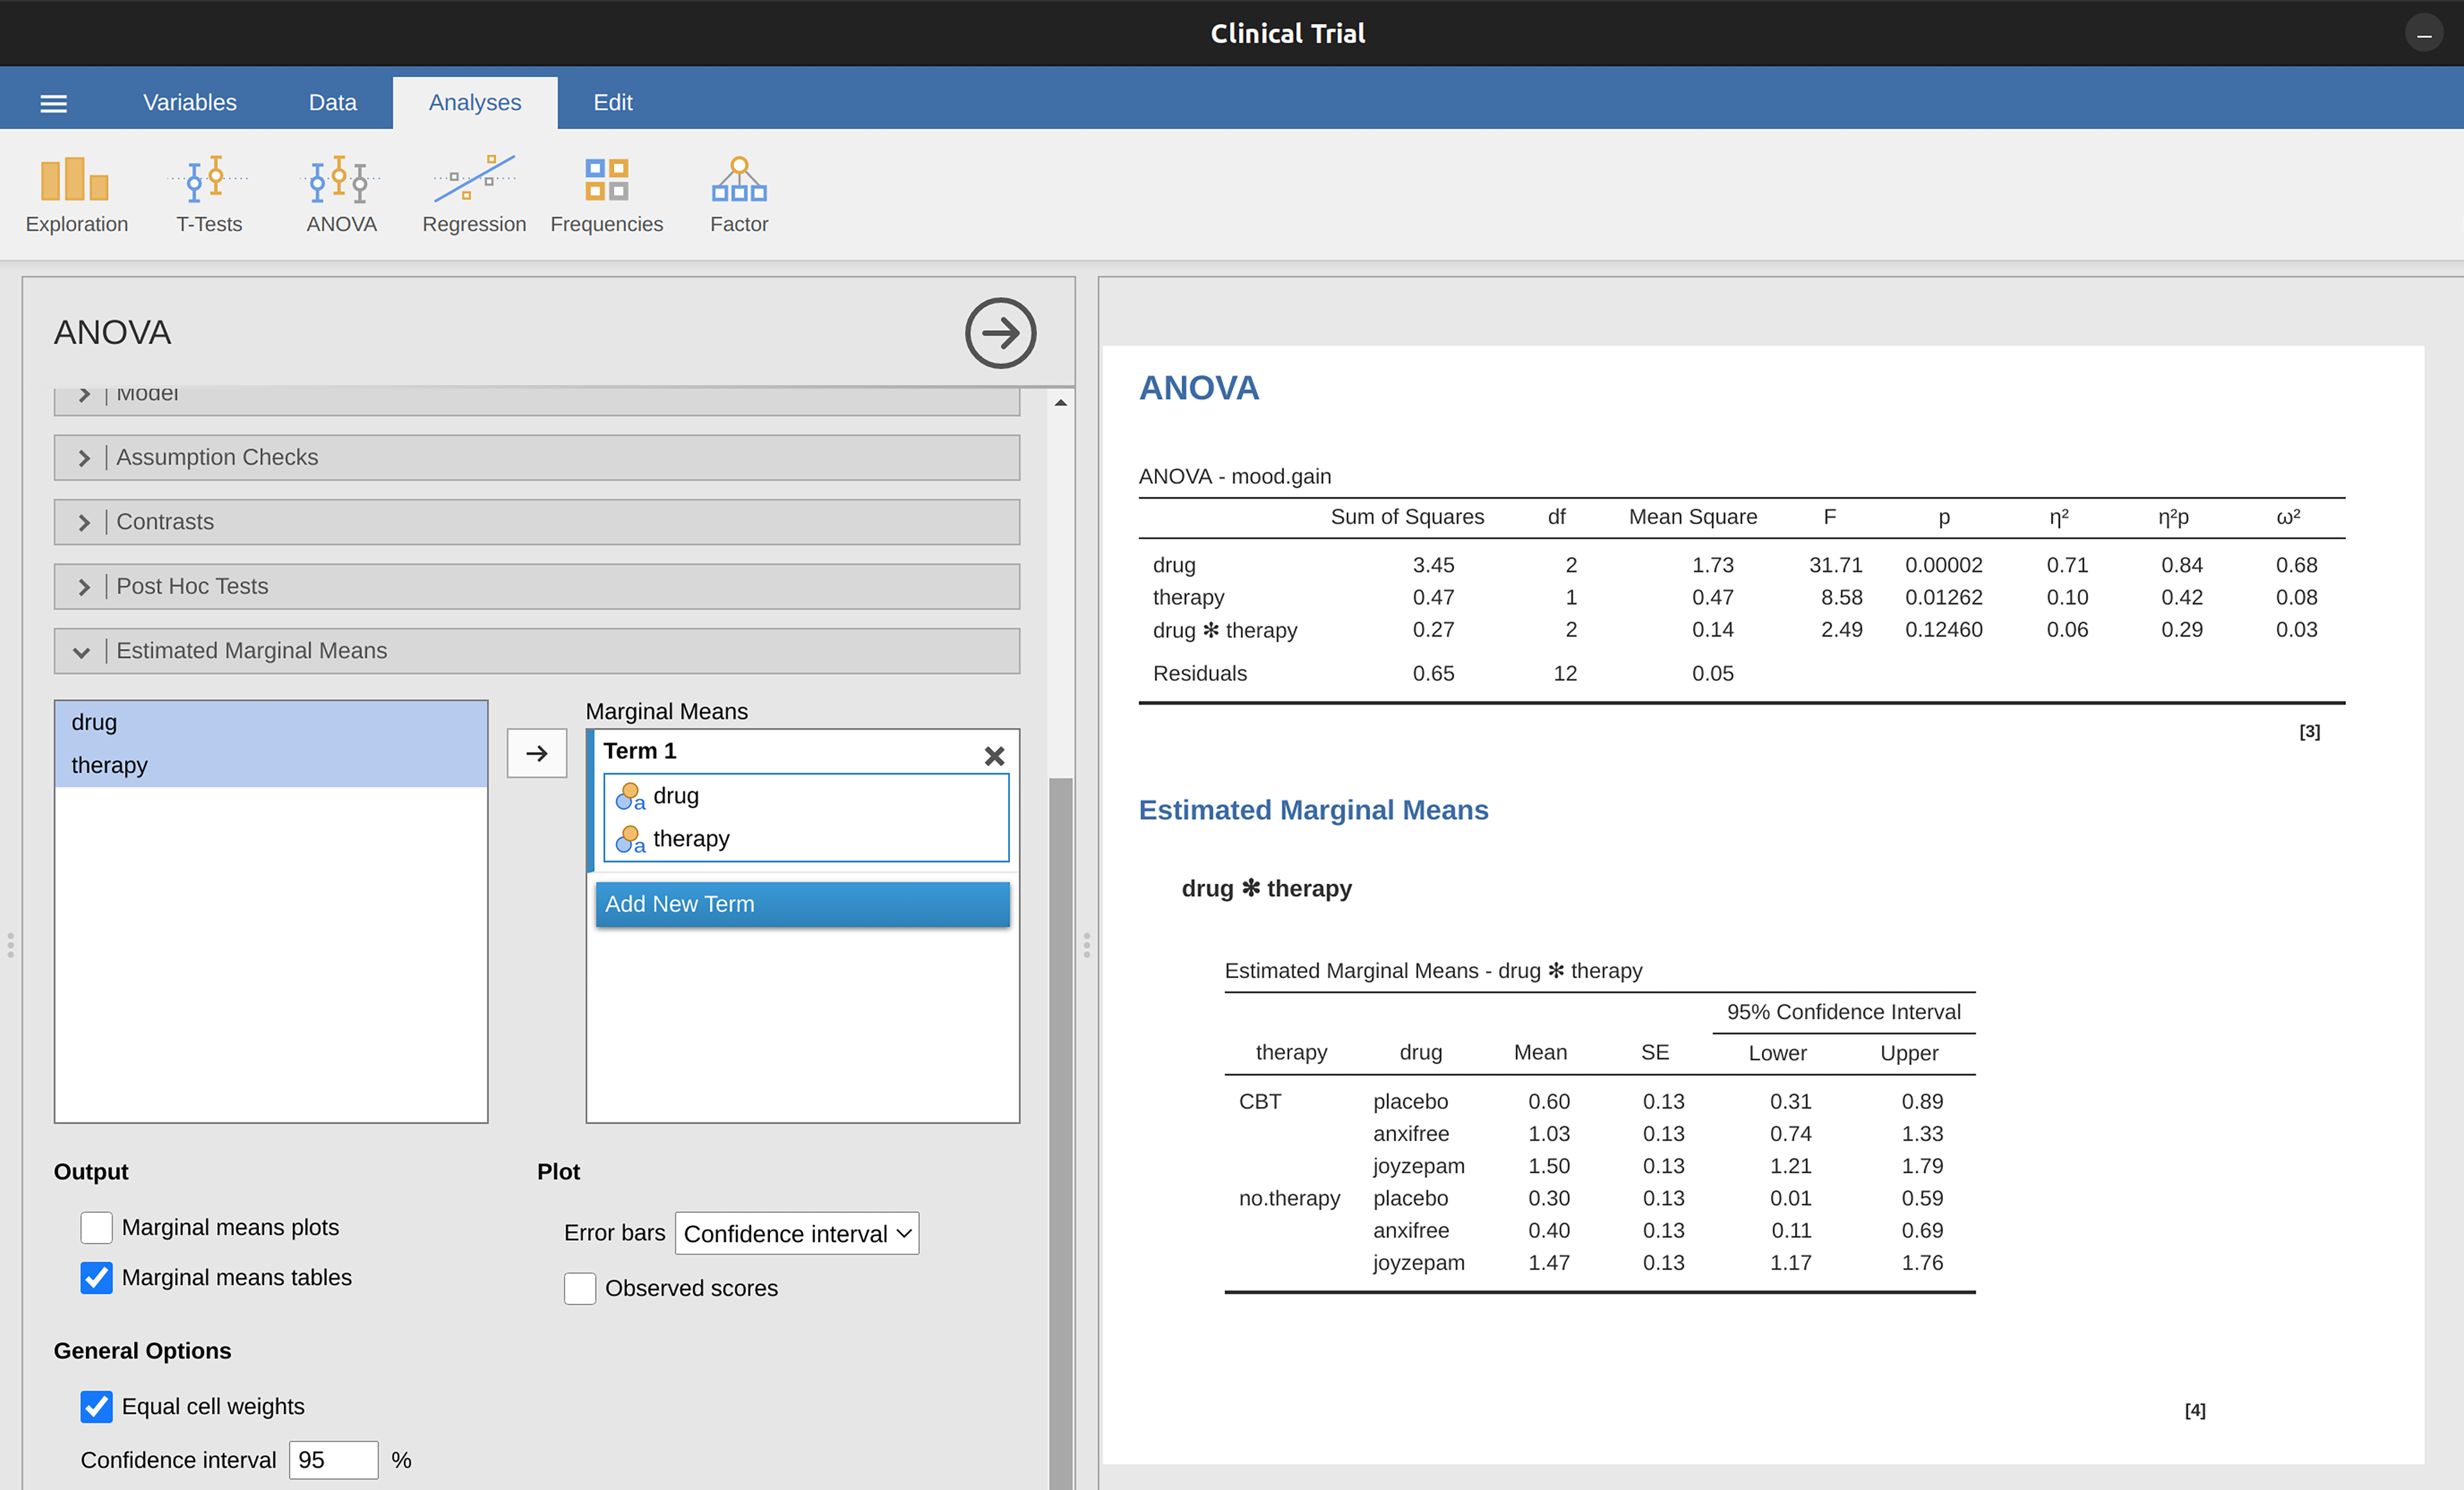
\includegraphics[width=1\textwidth,height=\textheight]{images/fig14-8.png} \hfill{}

\caption{\label{fig-fig14-8}jamovi screenshot showing the marginal means
for the saturated model, i.e.~including the interaction component, with
the clinical trial data set}

\end{figure}

In the output we see that the estimated mean mood gain for the placebo
group with no therapy was \(0.300\), with a \(95\%\) confidence interval
from \(0.006\) to \(0.594\). Note that these are not the same confidence
intervals that you would get if you calculated them separately for each
group, because of the fact that the ANOVA model assumes homogeneity of
variance and therefore uses a pooled estimate of the standard deviation.

When the model doesn't contain the interaction term, then the estimated
group means will be different from the sample means. Instead of
reporting the sample mean, jamovi will calculate the value of the group
means that would be expected on the basis of the marginal means (i.e.,
assuming no interaction). Using the notation we developed earlier, the
estimate reported for \(\mu_{rc}\), the mean for level \(r\) on the
(row) Factor A and level \(c\) on the (column) Factor B would be
\(\mu_{..} + \alpha_r + \beta_c\). If there are genuinely no
interactions between the two factors, this is actually a better estimate
of the population mean than the raw sample mean would be. Removing the
interaction term from the model, via the `Model' options in the jamovi
ANOVA analysis, provides the marginal means for the analysis shown in
Figure~\ref{fig-fig14-9}.

\begin{figure}

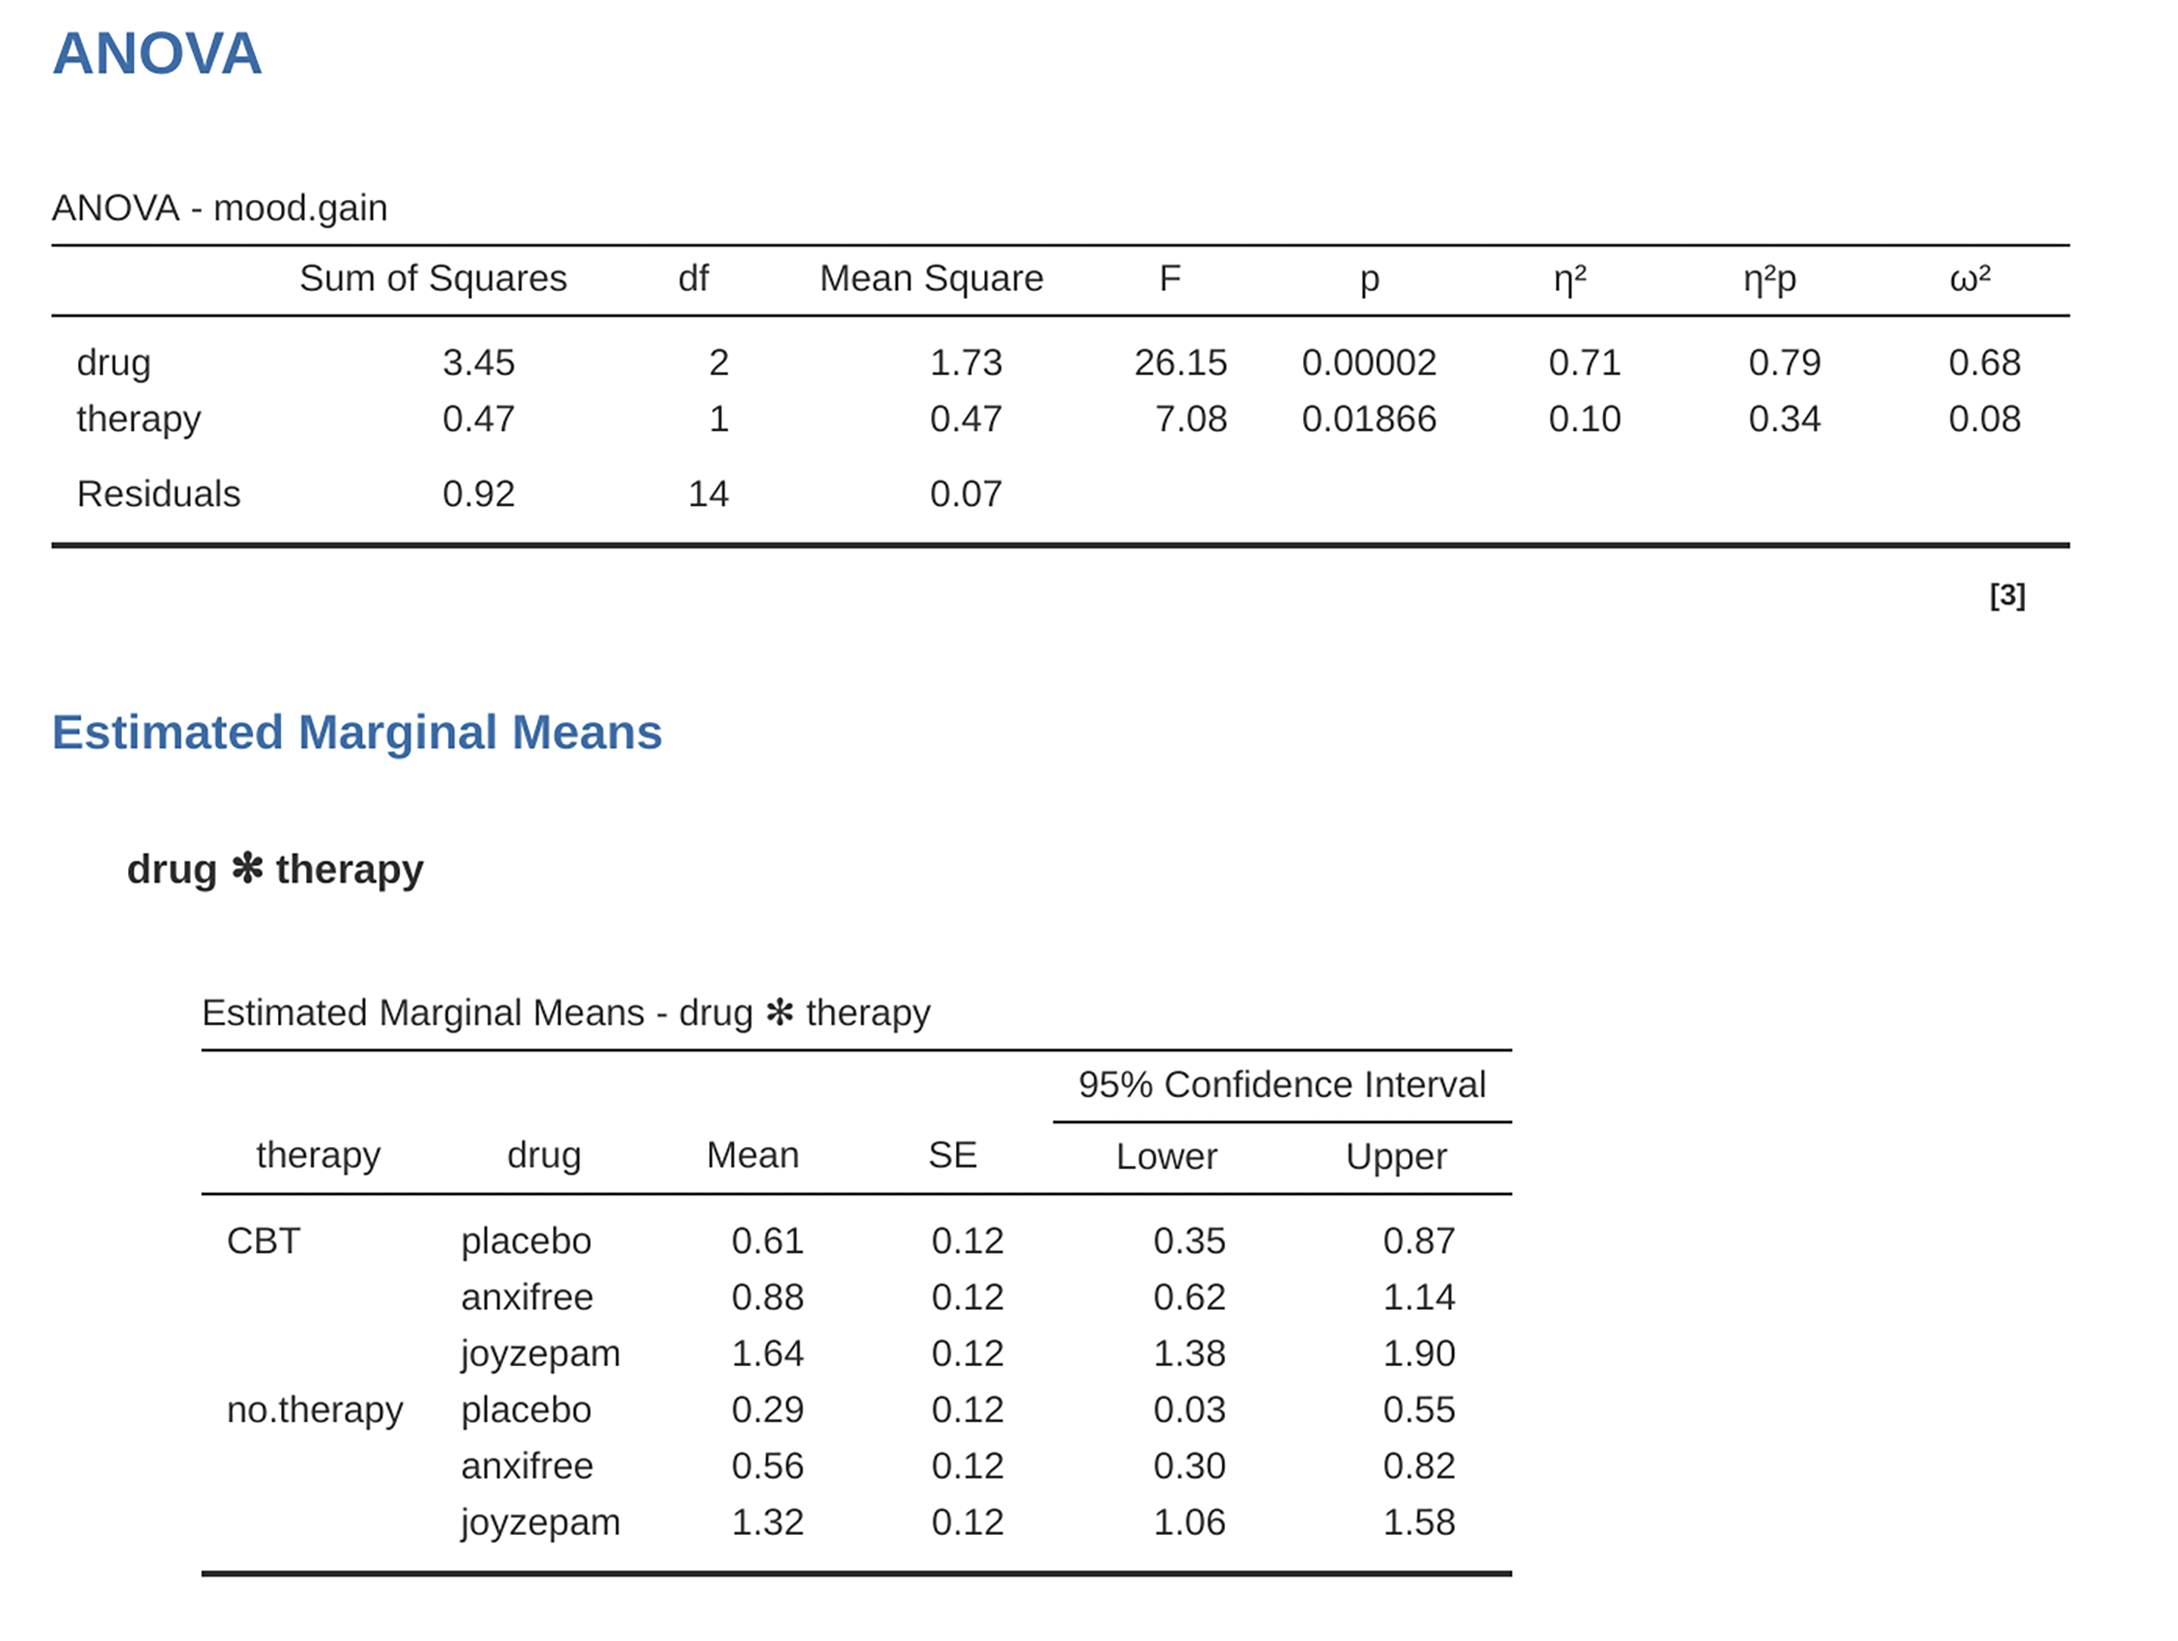
\includegraphics[width=1\textwidth,height=\textheight]{images/fig14-9.png} \hfill{}

\caption{\label{fig-fig14-9}jamovi screenshot showing the marginal means
for the unsaturated model, i.e.~without the interaction component, with
the clinical trial data set}

\end{figure}

\hypertarget{assumption-checking}{%
\section{Assumption checking}\label{assumption-checking}}

As with one-way ANOVA, the key assumptions of factorial ANOVA are
homogeneity of variance (all groups have the same standard deviation),
normality of the residuals, and independence of the observations. The
first two are things we can check for. The third is something that you
need to assess yourself by asking if there are any special relationships
between different observations, for example repeated measures where the
independent variable is time so there is a relationship between the
observations at time one and time two: observations at different time
points are from the same people. Additionally, if you aren't using a
saturated model (e.g., if you've omitted the interaction terms) then
you're also assuming that the omitted terms aren't important. Of course,
you can check this last one by running an ANOVA with the omitted terms
included and see if they're significant, so that's pretty easy. What
about homogeneity of variance and normality of the residuals? As it
turns out, these are pretty easy to check. It's no different to the
checks we did for a one-way ANOVA.

\hypertarget{homogeneity-of-variance}{%
\subsection{Homogeneity of variance}\label{homogeneity-of-variance}}

As mentioned in
\textbf{?@sec-Checking-the-homogeneity-of-variance-assumption} in the
last chapter, it's a good idea to visually inspect a plot of the
standard deviations compared across different groups / categories, and
also see if the Levene test is consistent with the visual inspection.
The theory behind the Levene test was discussed in
\textbf{?@sec-Checking-the-homogeneity-of-variance-assumption}, so I
won't discuss it again. This test expects that you have a saturated
model (i.e., including all of the relevant terms), because the test is
primarily concerned with the within-group variance, and it doesn't
really make a lot of sense to calculate this any way other than with
respect to the full model. The Levene test can be specified under the
ANOVA `Assumption Checks' - `Homogeneity Tests' option in jamovi, with
the result shown as in Figure~\ref{fig-fig14-10}. The fact that the
Levene test is non-significant means that, providing it is consistent
with a visual inspection of the plot of standard deviations, we can
safely assume that the homogeneity of variance assumption is not
violated.

\hypertarget{normality-of-residuals}{%
\subsection{Normality of residuals}\label{normality-of-residuals}}

As with one-way ANOVA we can test for the normality of residuals in a
straightforward fashion (see
\textbf{?@sec-Checking-the-normality-assumption}). Primarily though,
it's generally a good idea to examine the residuals graphically using a
QQ plot. See Figure~\ref{fig-fig14-10}.

\begin{figure}

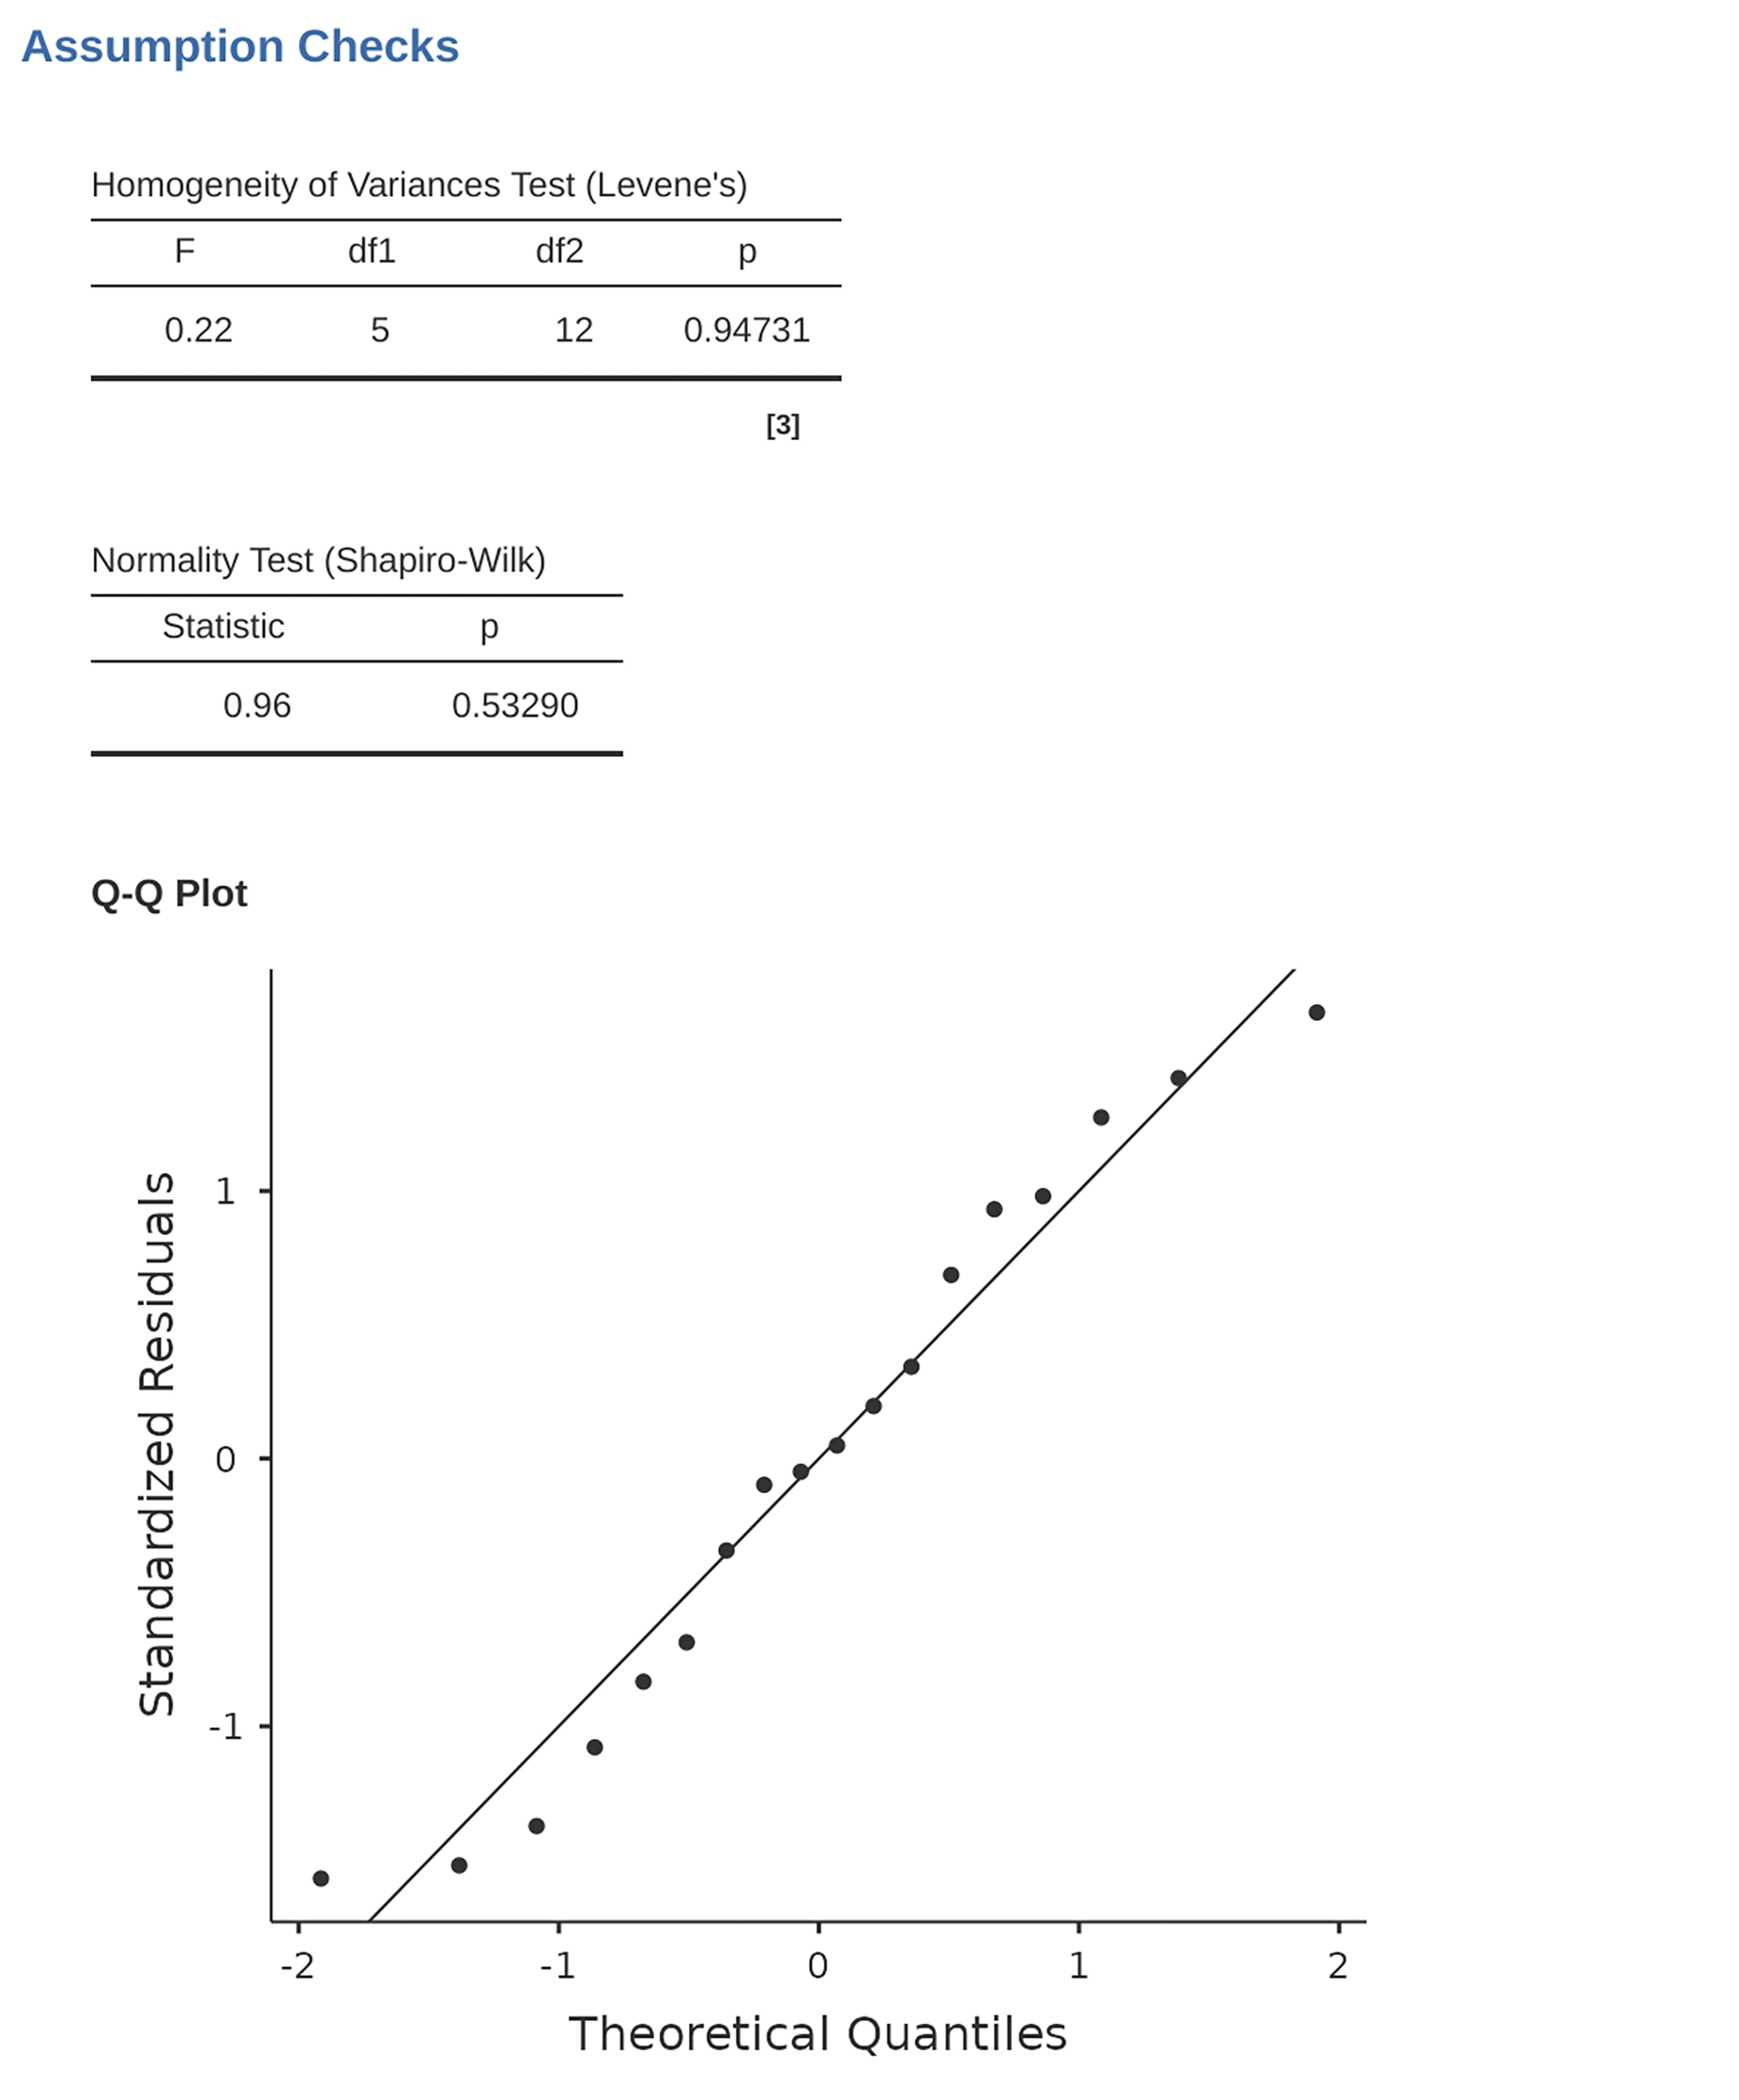
\includegraphics[width=1\textwidth,height=\textheight]{images/fig14-10.png} \hfill{}

\caption{\label{fig-fig14-10}Checking assumptions in an ANOVA model}

\end{figure}

\hypertarget{sec-analysis-of-covariance-ancova}{%
\section{Analysis of covariance
(ANCOVA)}\label{sec-analysis-of-covariance-ancova}}

A variation in ANOVA is when you have an additional continuous variable
that you think might be related to the dependent variable. This
additional variable can be added to the analysis as a covariate, in the
aptly named analysis of covariance (ANCOVA).

In ANCOVA the values of the dependent variable are ``adjusted'' for the
influence of the covariate, and then the ``adjusted'' score means are
tested between groups in the usual way. This technique can increase the
precision of an experiment, and therefore provide a more ``powerful''
test of the equality of group means in the dependent variable. How does
ANCOVA do this? Well, although the covariate itself is typically not of
any experimental interest, adjustment for the covariate can decrease the
estimate of experimental error and thus, by reducing error variance,
precision is increased. This means that an inappropriate failure to
reject the null hypothesis (false negative or type II error) is less
likely.

Despite this advantage, ANCOVA runs the risk of undoing real differences
between groups, and this should be avoided. Look at
Figure~\ref{fig-fig14-11}, for example, which shows a plot of Statistics
anxiety against age and shows two distinct groups -- students who have
either an Arts or Science background or preference. ANCOVA with age as a
covariate might lead to the conclusion that statistics anxiety does not
differ in the two groups. Would this conclusion be reasonable --
probably not because the ages of the two groups do not overlap and
analysis of variance has essentially ``extrapolated into a region with
no data'' (Everitt (1996), p.~68).

\begin{figure}


\includegraphics[width=1\textwidth,height=\textheight]{images/fig14-11.png} \hfill{}

\caption{\label{fig-fig14-11}Plot of Statistics anxiety against age for
two distinct groups}

\end{figure}

Clearly, careful thought needs to be given to an analysis of covariance
with distinct groups. This applies to both one-way and factorial
designs, as ANCOVA can be used with both.

\hypertarget{running-ancova-in-jamovi}{%
\subsection{Running ANCOVA in jamovi}\label{running-ancova-in-jamovi}}

A health psychologist was interested in the effect of routine cycling
and stress on happiness levels, with age as a covariate. You can find
the dataset in the file \emph{ancova.csv}. Open this file in jamovi and
then, to undertake an ANCOVA, select Analyses - ANOVA - ANCOVA to open
the ANCOVA analysis window (Figure~\ref{fig-fig14-12}). Highlight the
dependent variable `happiness' and transfer it into the `Dependent
Variable' text box. Highlight the independent variables `stress' and
`commute' and transfer them into the `Fixed Factors' text box. Highlight
the covariate `age' and transfer it into the `Covariates' text box. Then
click on Estimated Marginal Means to bring up the plots and tables
options.

\begin{figure}

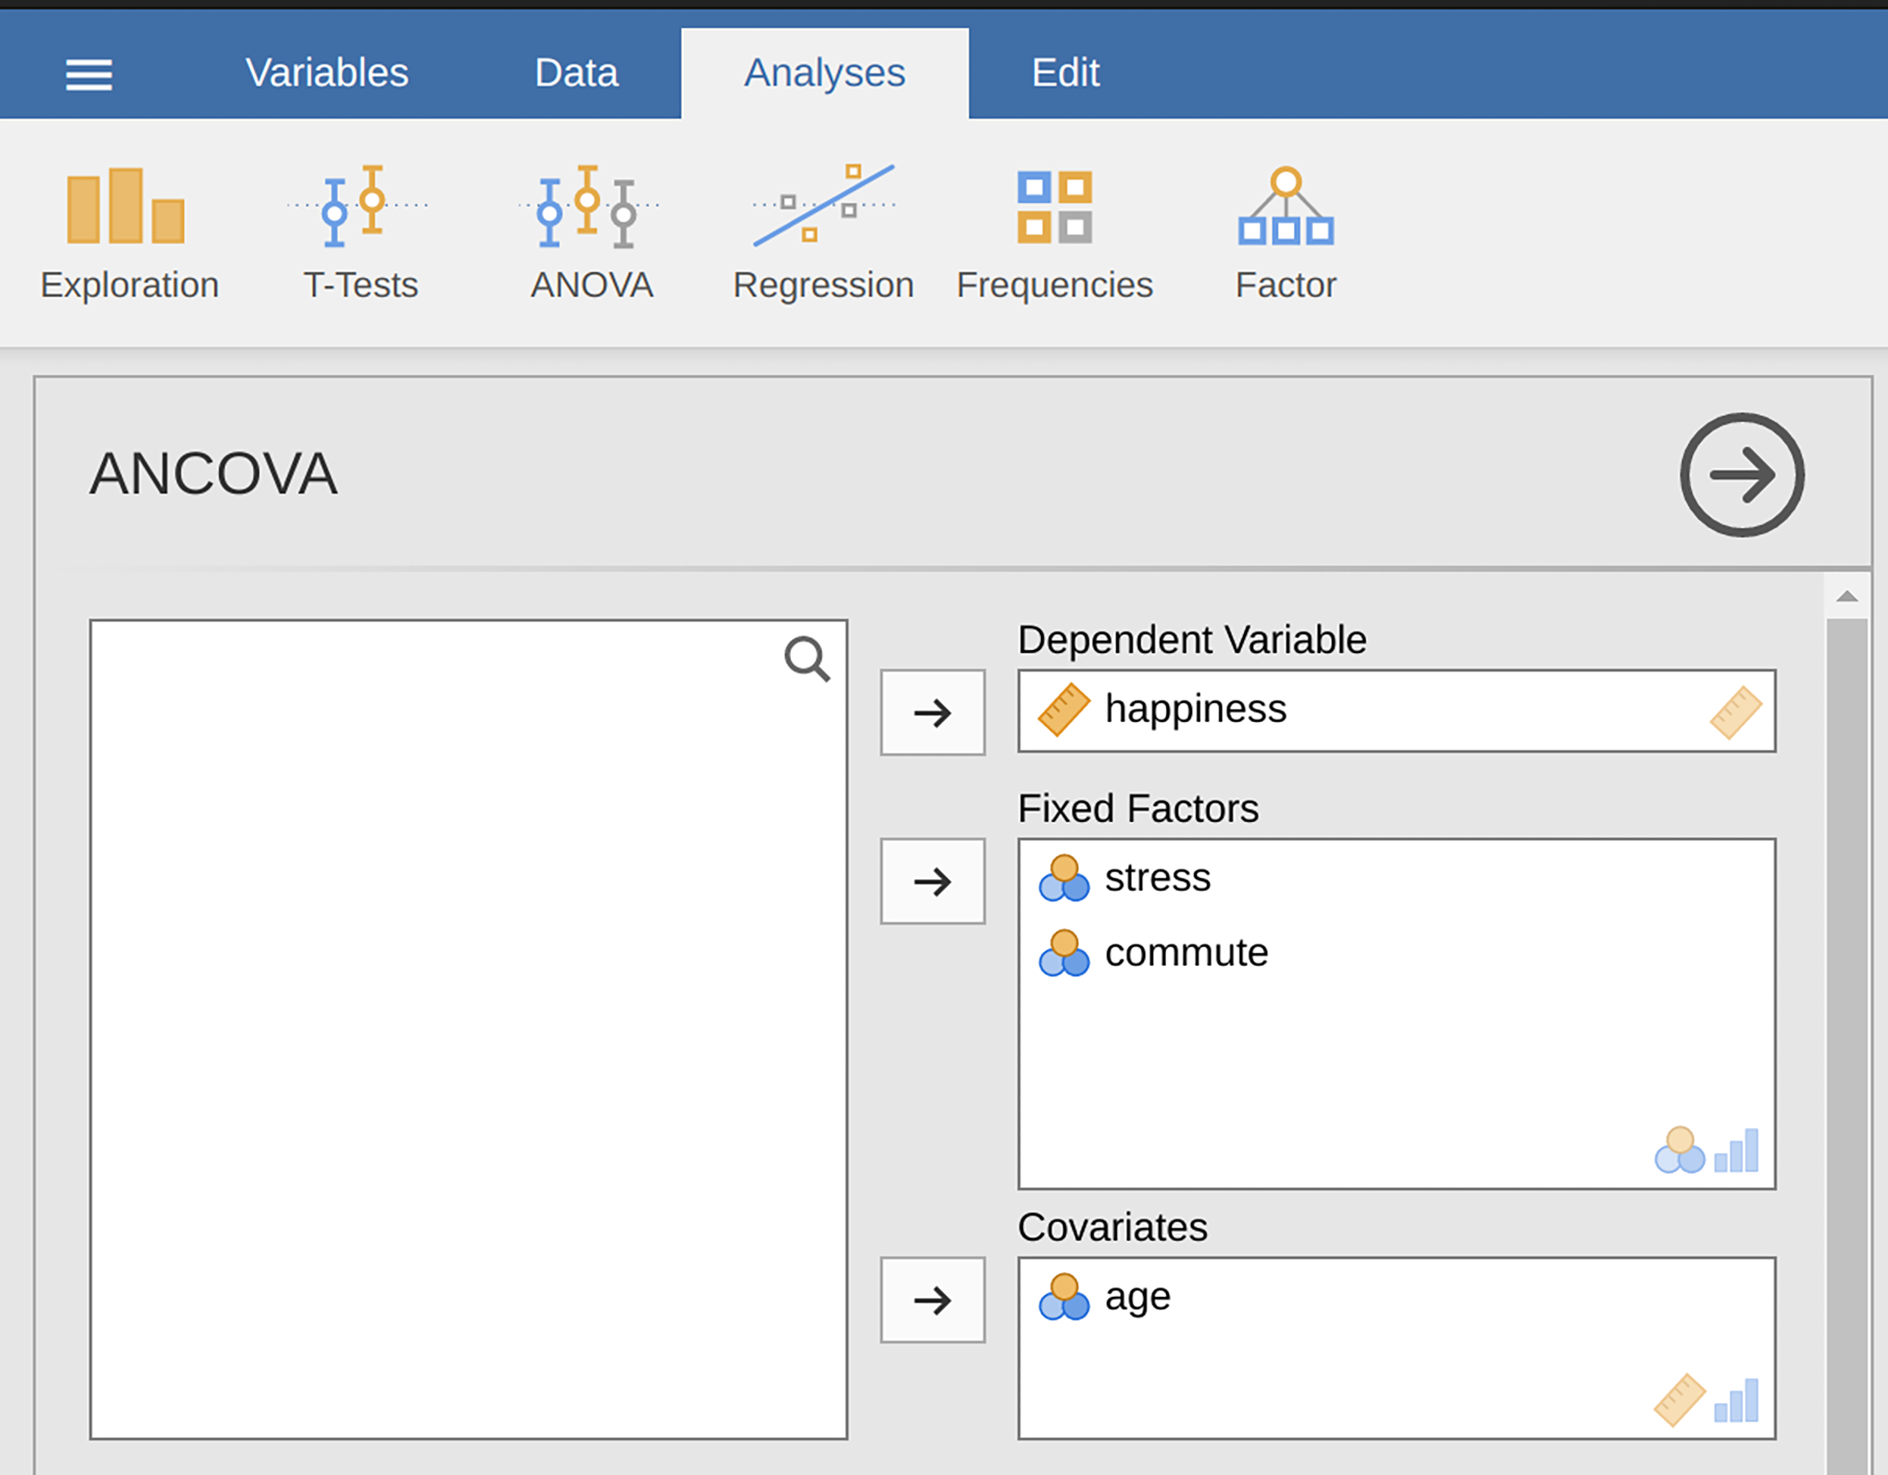
\includegraphics[width=1\textwidth,height=\textheight]{images/fig14-12.png} \hfill{}

\caption{\label{fig-fig14-12}The jamovi ANCOVA analysis window}

\end{figure}

An ANCOVA table showing `Tests of Between Subjects Effects' is produced
in the jamovi results window (Figure~\ref{fig-fig14-13}). The
\(F\)-value for the covariate `age' is significant at \(p = .023\),
suggesting that age is an important predictor of the dependent variable,
happiness. When we look at the estimated marginal mean scores
(Figure~\ref{fig-fig14-14}), adjustments have been made (compared to an
analysis without the covariate) because of the inclusion of the
covariate `age' in this ANCOVA. A plot (Figure~\ref{fig-fig14-15}) is a
good way of visualising and interpreting the significant effects.

\begin{figure}

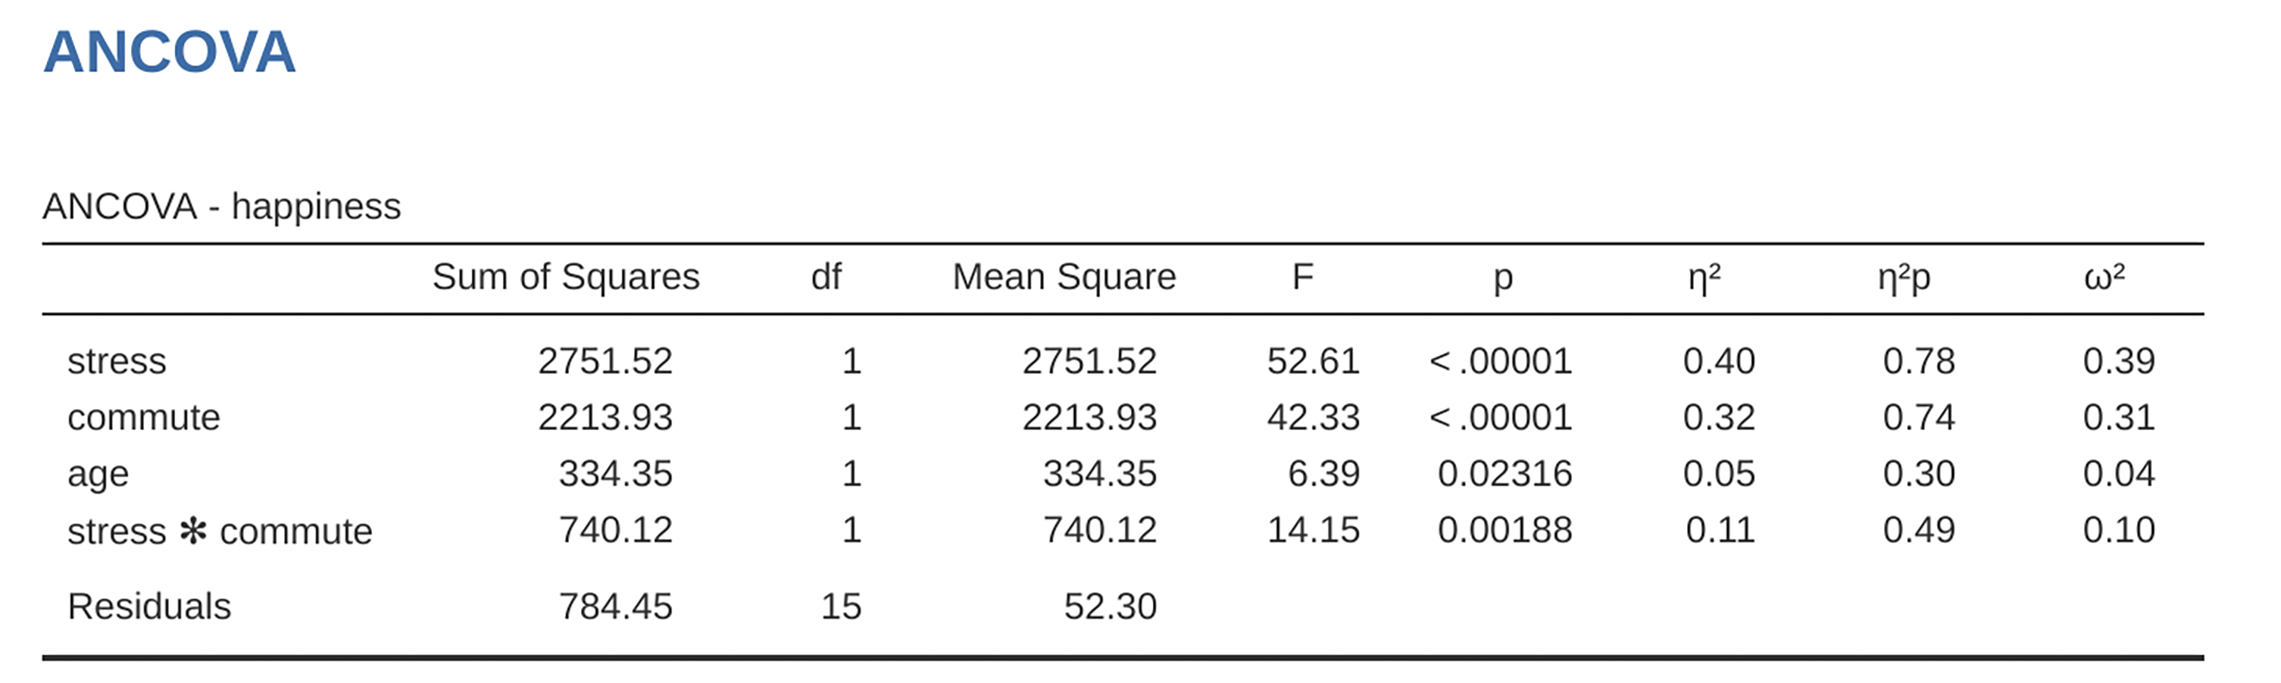
\includegraphics[width=1\textwidth,height=\textheight]{images/fig14-13.png} \hfill{}

\caption{\label{fig-fig14-13}jamovi ANCOVA output for happiness as a
function of stress and commuting method, with age as a covariate}

\end{figure}

\begin{figure}

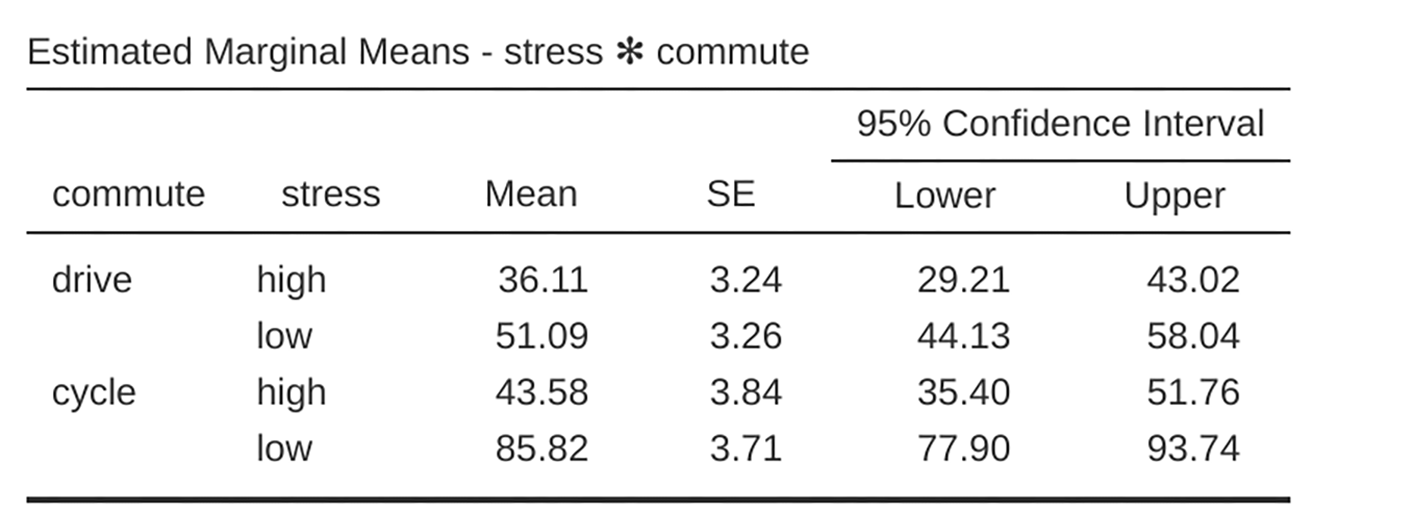
\includegraphics[width=1\textwidth,height=\textheight]{images/fig14-14.png} \hfill{}

\caption{\label{fig-fig14-14}Table of mean happiness level as a function
of stress and commuting method (adjusted for the covariate age) with
95\% confidence intervals}

\end{figure}

The \(F\)-value for the main effect `stress' (52.61) has an associated
probability of \(p < .001\). The \(F\)-value for the main effect
`commute' (42.33) has an associated probability of \(p < .001\). Since
both of these are less than the probability that is typically used to
decide if a statistical result is significant (\(p < .05\)) we can
conclude that there was a significant main effect of stress
(\(F(1, 15) = 52.61, p < .001\)) and a significant main effect of
commuting method (\(F(1, 15) = 42.33, p < .001\)). A significant
interaction between stress and commuting method was also found
(\(F(1, 15) = 14.15, p = .002\)).

In Figure~\ref{fig-fig14-15} we can see the adjusted, marginal, mean
happiness scores when age is a covariate in an ANCOVA. In this analysis
there is a significant interaction effect, whereby people with low
stress who cycle to work are happier than people with low stress who
drive and people with high stress regardless of whether they cycle or
drive to work. There is also a significant main effect of stress --
people with low stress are happier than those with high stress. And
there is also a significant main effect of commuting behaviour -- people
who cycle are happier, on average, than those who drive to work.

\begin{figure}


\includegraphics[width=1\textwidth,height=\textheight]{images/fig14-15.png} \hfill{}

\caption{\label{fig-fig14-15}Plot of mean happiness level as a function
of stress and commuting method}

\end{figure}

One thing to be aware of is that, if you are thinking of including a
covariate in your ANOVA, there is an additional assumption: the
relationship between the covariate and the dependent variable should be
similar for all levels of the independent variable. This can be checked
by adding an interaction term between the covariate and each independent
variable in the jamovi `Model - Model' terms option. If the interaction
effect is not significant it can be removed. If it is significant then a
different and more advanced statistical technique might be appropriate
(which is beyond the scope of this book so you might want to consult a
friendly statistician).

\hypertarget{sec-ANOVA-as-a-linear-model}{%
\section{ANOVA as a linear model}\label{sec-ANOVA-as-a-linear-model}}

One of the most important things to understand about ANOVA and
regression is that they're basically the same thing. On the surface of
it, you maybe wouldn't think this is true. After all, the way that I've
described them so far suggests that ANOVA is primarily concerned with
testing for group differences, and regression is primarily concerned
with understanding the correlations between variables. And, as far as it
goes that's perfectly true. But when you look under the hood, so to
speak, the underlying mechanics of ANOVA and regression are awfully
similar. In fact, if you think about it, you've already seen evidence of
this. ANOVA and regression both rely heavily on sums of squares
(\(SS\)), both make use of \(F\)-tests, and so on. Looking back, it's
hard to escape the feeling that
\textbf{?@sec-Correlation-and-linear-regression} and
\textbf{?@sec-Comparing-several-means-one-way-ANOVA} were a bit
repetitive.

The reason for this is that ANOVA and regression are both kinds of
\textbf{linear models}. In the case of regression, this is kind of
obvious. The regression equation that we use to define the relationship
between predictors and outcomes is the equation for a straight line, so
it's quite obviously a linear model, with the equation:

\[Y_p=b_0+b_1 X_{1p} +b_2 X_{2p} + \epsilon_p\]

where \(Y_p\) is the outcome value for the \(p\)-th observation (e.g.,
\(p\)-th person), \(X_{1p}\) is the value of the first predictor for the
\(p\)-th observation, \(X_{2p}\) is the value of the second predictor
for the \(p\)-th observation, the \(b_0\), \(b_1\), and \(b_2\) terms
are our regression coefficients, and \(\epsilon_p\) is the \(p\)-th
residual. If we ignore the residuals \(\epsilon_p\) and just focus on
the regression line itself, we get the following formula:

\[\hat{Y}_p=b_0+b_1 X_{1p} +b_2 X_{2p} \]

where \(\hat{Y}_p\) is the value of Y that the regression line predicts
for person p, as opposed to the actually-observed value \(Y_p\). The
thing that isn't immediately obvious is that we can write ANOVA as a
linear model as well. However, it's actually pretty straightforward to
do this. Let's start with a really simple example, rewriting a
\(2 \times 2\) factorial ANOVA as a linear model.

\hypertarget{some-data}{%
\subsection{Some data}\label{some-data}}

To make things concrete, let's suppose that our outcome variable is the
grade that a student receives in my class, a ratio-scale variable
corresponding to a mark from \(0%
\) to \(100%
\). There are two predictor variables of interest: whether or not the
student turned up to lectures (the attend variable) and whether or not
the student actually read the textbook (the reading variable). We'll say
that attend = 1 if the student attended class, and attend = 0 if they
did not. Similarly, we'll say that reading = 1 if the student read the
textbook, and reading = 0 if they did not.

Okay, so far that's simple enough. The next thing we need to do is to
wrap some maths around this (sorry!). For the purposes of this example,
let \(Y_p\) denote the grade of the \(p\)-th student in the class. This
is not quite the same notation that we used earlier in this chapter.
Previously, we've used the notation \(Y_{rci}\) to refer to the \(i\)-th
person in the \(r\)-th group for predictor 1 (the row factor) and the
\(c\)-th group for predictor 2 (the column factor). This extended
notation was really handy for describing how the \(SS\) values are
calculated, but it's a pain in the current context, so I'll switch
notation here. Now, the \(Y_p\) notation is visually simpler than
\(Y_{rci}\), but it has the shortcoming that it doesn't actually keep
track of the group memberships! That is, if I told you that
\(Y_{0,0,3} = 35\), you'd immediately know that we're talking about a
student (the 3rd such student, in fact) who didn't attend the lectures
(i.e., attend = 0) and didn't read the textbook (i.e.~reading = 0), and
who ended up failing the class (grade = 35). But if I tell you that
\(Y_p = 35\), all you know is that the \(p\)-th student didn't get a
good grade. We've lost some key information here. Of course, it doesn't
take a lot of thought to figure out how to fix this. What we'll do
instead is introduce two new variables \(X_{1p}\) and \(X_{2p}\) that
keep track of this information. In the case of our hypothetical student,
we know that \(X_{1p} = 0\) (i.e., attend = 0) and \(X_{2p} = 0\) (i.e.,
reading = 0). So the data might look like Table~\ref{tbl-tab14-8}.

\hypertarget{tbl-tab14-8}{}
 
  \providecommand{\huxb}[2]{\arrayrulecolor[RGB]{#1}\global\arrayrulewidth=#2pt}
  \providecommand{\huxvb}[2]{\color[RGB]{#1}\vrule width #2pt}
  \providecommand{\huxtpad}[1]{\rule{0pt}{#1}}
  \providecommand{\huxbpad}[1]{\rule[-#1]{0pt}{#1}}

\begin{table}[ht]
\caption{\label{tbl-tab14-8}Data for grade, attendance and reading the textbook }\tabularnewline

\begin{centerbox}
\begin{threeparttable}
\setlength{\tabcolsep}{0pt}
\begin{tabularx}{0.9\textwidth}{p{0.225\textwidth} p{0.225\textwidth} p{0.225\textwidth} p{0.225\textwidth}}


\hhline{>{\huxb{0, 0, 0}{0.4}}->{\huxb{0, 0, 0}{0.4}}->{\huxb{0, 0, 0}{0.4}}->{\huxb{0, 0, 0}{0.4}}-}
\arrayrulecolor{black}

\multicolumn{1}{!{\huxvb{0, 0, 0}{0}}p{0.225\textwidth}!{\huxvb{0, 0, 0}{0}}}{\hspace{0pt}\parbox[b]{0.225\textwidth-0pt-12pt}{\huxtpad{2pt + 1em}\centering \textbf{person, \(p\)}\huxbpad{2pt}}} &
\multicolumn{1}{p{0.225\textwidth}!{\huxvb{0, 0, 0}{0}}}{\hspace{12pt}\parbox[b]{0.225\textwidth-12pt-12pt}{\huxtpad{2pt + 1em}\centering \textbf{grade, \(Y_p\)}\huxbpad{2pt}}} &
\multicolumn{1}{p{0.225\textwidth}!{\huxvb{0, 0, 0}{0}}}{\hspace{12pt}\parbox[b]{0.225\textwidth-12pt-12pt}{\huxtpad{2pt + 1em}\centering \textbf{attendance, \(X_{1p}\)}\huxbpad{2pt}}} &
\multicolumn{1}{p{0.225\textwidth}!{\huxvb{0, 0, 0}{0}}}{\hspace{12pt}\parbox[b]{0.225\textwidth-12pt-0pt}{\huxtpad{2pt + 1em}\centering \textbf{reading, \(X_{2p}\)}\huxbpad{2pt}}} \tabularnewline[-0.5pt]


\hhline{>{\huxb{0, 0, 0}{0.4}}->{\huxb{0, 0, 0}{0.4}}->{\huxb{0, 0, 0}{0.4}}->{\huxb{0, 0, 0}{0.4}}-}
\arrayrulecolor{black}

\multicolumn{1}{!{\huxvb{0, 0, 0}{0}}p{0.225\textwidth}!{\huxvb{0, 0, 0}{0}}}{\hspace{0pt}\parbox[b]{0.225\textwidth-0pt-12pt}{\huxtpad{2pt + 1em}\centering 1\huxbpad{2pt}}} &
\multicolumn{1}{p{0.225\textwidth}!{\huxvb{0, 0, 0}{0}}}{\hspace{12pt}\parbox[b]{0.225\textwidth-12pt-12pt}{\huxtpad{2pt + 1em}\centering 90\huxbpad{2pt}}} &
\multicolumn{1}{p{0.225\textwidth}!{\huxvb{0, 0, 0}{0}}}{\hspace{12pt}\parbox[b]{0.225\textwidth-12pt-12pt}{\huxtpad{2pt + 1em}\centering 1\huxbpad{2pt}}} &
\multicolumn{1}{p{0.225\textwidth}!{\huxvb{0, 0, 0}{0}}}{\hspace{12pt}\parbox[b]{0.225\textwidth-12pt-0pt}{\huxtpad{2pt + 1em}\centering 1\huxbpad{2pt}}} \tabularnewline[-0.5pt]


\hhline{}
\arrayrulecolor{black}

\multicolumn{1}{!{\huxvb{0, 0, 0}{0}}p{0.225\textwidth}!{\huxvb{0, 0, 0}{0}}}{\hspace{0pt}\parbox[b]{0.225\textwidth-0pt-12pt}{\huxtpad{2pt + 1em}\centering 2\huxbpad{2pt}}} &
\multicolumn{1}{p{0.225\textwidth}!{\huxvb{0, 0, 0}{0}}}{\hspace{12pt}\parbox[b]{0.225\textwidth-12pt-12pt}{\huxtpad{2pt + 1em}\centering 87\huxbpad{2pt}}} &
\multicolumn{1}{p{0.225\textwidth}!{\huxvb{0, 0, 0}{0}}}{\hspace{12pt}\parbox[b]{0.225\textwidth-12pt-12pt}{\huxtpad{2pt + 1em}\centering 1\huxbpad{2pt}}} &
\multicolumn{1}{p{0.225\textwidth}!{\huxvb{0, 0, 0}{0}}}{\hspace{12pt}\parbox[b]{0.225\textwidth-12pt-0pt}{\huxtpad{2pt + 1em}\centering 1\huxbpad{2pt}}} \tabularnewline[-0.5pt]


\hhline{}
\arrayrulecolor{black}

\multicolumn{1}{!{\huxvb{0, 0, 0}{0}}p{0.225\textwidth}!{\huxvb{0, 0, 0}{0}}}{\hspace{0pt}\parbox[b]{0.225\textwidth-0pt-12pt}{\huxtpad{2pt + 1em}\centering 3\huxbpad{2pt}}} &
\multicolumn{1}{p{0.225\textwidth}!{\huxvb{0, 0, 0}{0}}}{\hspace{12pt}\parbox[b]{0.225\textwidth-12pt-12pt}{\huxtpad{2pt + 1em}\centering 75\huxbpad{2pt}}} &
\multicolumn{1}{p{0.225\textwidth}!{\huxvb{0, 0, 0}{0}}}{\hspace{12pt}\parbox[b]{0.225\textwidth-12pt-12pt}{\huxtpad{2pt + 1em}\centering 0\huxbpad{2pt}}} &
\multicolumn{1}{p{0.225\textwidth}!{\huxvb{0, 0, 0}{0}}}{\hspace{12pt}\parbox[b]{0.225\textwidth-12pt-0pt}{\huxtpad{2pt + 1em}\centering 1\huxbpad{2pt}}} \tabularnewline[-0.5pt]


\hhline{}
\arrayrulecolor{black}

\multicolumn{1}{!{\huxvb{0, 0, 0}{0}}p{0.225\textwidth}!{\huxvb{0, 0, 0}{0}}}{\hspace{0pt}\parbox[b]{0.225\textwidth-0pt-12pt}{\huxtpad{2pt + 1em}\centering 4\huxbpad{2pt}}} &
\multicolumn{1}{p{0.225\textwidth}!{\huxvb{0, 0, 0}{0}}}{\hspace{12pt}\parbox[b]{0.225\textwidth-12pt-12pt}{\huxtpad{2pt + 1em}\centering 60\huxbpad{2pt}}} &
\multicolumn{1}{p{0.225\textwidth}!{\huxvb{0, 0, 0}{0}}}{\hspace{12pt}\parbox[b]{0.225\textwidth-12pt-12pt}{\huxtpad{2pt + 1em}\centering 1\huxbpad{2pt}}} &
\multicolumn{1}{p{0.225\textwidth}!{\huxvb{0, 0, 0}{0}}}{\hspace{12pt}\parbox[b]{0.225\textwidth-12pt-0pt}{\huxtpad{2pt + 1em}\centering 0\huxbpad{2pt}}} \tabularnewline[-0.5pt]


\hhline{}
\arrayrulecolor{black}

\multicolumn{1}{!{\huxvb{0, 0, 0}{0}}p{0.225\textwidth}!{\huxvb{0, 0, 0}{0}}}{\hspace{0pt}\parbox[b]{0.225\textwidth-0pt-12pt}{\huxtpad{2pt + 1em}\centering 5\huxbpad{2pt}}} &
\multicolumn{1}{p{0.225\textwidth}!{\huxvb{0, 0, 0}{0}}}{\hspace{12pt}\parbox[b]{0.225\textwidth-12pt-12pt}{\huxtpad{2pt + 1em}\centering 35\huxbpad{2pt}}} &
\multicolumn{1}{p{0.225\textwidth}!{\huxvb{0, 0, 0}{0}}}{\hspace{12pt}\parbox[b]{0.225\textwidth-12pt-12pt}{\huxtpad{2pt + 1em}\centering 0\huxbpad{2pt}}} &
\multicolumn{1}{p{0.225\textwidth}!{\huxvb{0, 0, 0}{0}}}{\hspace{12pt}\parbox[b]{0.225\textwidth-12pt-0pt}{\huxtpad{2pt + 1em}\centering 0\huxbpad{2pt}}} \tabularnewline[-0.5pt]


\hhline{}
\arrayrulecolor{black}

\multicolumn{1}{!{\huxvb{0, 0, 0}{0}}p{0.225\textwidth}!{\huxvb{0, 0, 0}{0}}}{\hspace{0pt}\parbox[b]{0.225\textwidth-0pt-12pt}{\huxtpad{2pt + 1em}\centering 6\huxbpad{2pt}}} &
\multicolumn{1}{p{0.225\textwidth}!{\huxvb{0, 0, 0}{0}}}{\hspace{12pt}\parbox[b]{0.225\textwidth-12pt-12pt}{\huxtpad{2pt + 1em}\centering 50\huxbpad{2pt}}} &
\multicolumn{1}{p{0.225\textwidth}!{\huxvb{0, 0, 0}{0}}}{\hspace{12pt}\parbox[b]{0.225\textwidth-12pt-12pt}{\huxtpad{2pt + 1em}\centering 0\huxbpad{2pt}}} &
\multicolumn{1}{p{0.225\textwidth}!{\huxvb{0, 0, 0}{0}}}{\hspace{12pt}\parbox[b]{0.225\textwidth-12pt-0pt}{\huxtpad{2pt + 1em}\centering 0\huxbpad{2pt}}} \tabularnewline[-0.5pt]


\hhline{}
\arrayrulecolor{black}

\multicolumn{1}{!{\huxvb{0, 0, 0}{0}}p{0.225\textwidth}!{\huxvb{0, 0, 0}{0}}}{\hspace{0pt}\parbox[b]{0.225\textwidth-0pt-12pt}{\huxtpad{2pt + 1em}\centering 7\huxbpad{2pt}}} &
\multicolumn{1}{p{0.225\textwidth}!{\huxvb{0, 0, 0}{0}}}{\hspace{12pt}\parbox[b]{0.225\textwidth-12pt-12pt}{\huxtpad{2pt + 1em}\centering 65\huxbpad{2pt}}} &
\multicolumn{1}{p{0.225\textwidth}!{\huxvb{0, 0, 0}{0}}}{\hspace{12pt}\parbox[b]{0.225\textwidth-12pt-12pt}{\huxtpad{2pt + 1em}\centering 1\huxbpad{2pt}}} &
\multicolumn{1}{p{0.225\textwidth}!{\huxvb{0, 0, 0}{0}}}{\hspace{12pt}\parbox[b]{0.225\textwidth-12pt-0pt}{\huxtpad{2pt + 1em}\centering 0\huxbpad{2pt}}} \tabularnewline[-0.5pt]


\hhline{}
\arrayrulecolor{black}

\multicolumn{1}{!{\huxvb{0, 0, 0}{0}}p{0.225\textwidth}!{\huxvb{0, 0, 0}{0}}}{\hspace{0pt}\parbox[b]{0.225\textwidth-0pt-12pt}{\huxtpad{2pt + 1em}\centering 8\huxbpad{2pt}}} &
\multicolumn{1}{p{0.225\textwidth}!{\huxvb{0, 0, 0}{0}}}{\hspace{12pt}\parbox[b]{0.225\textwidth-12pt-12pt}{\huxtpad{2pt + 1em}\centering 70\huxbpad{2pt}}} &
\multicolumn{1}{p{0.225\textwidth}!{\huxvb{0, 0, 0}{0}}}{\hspace{12pt}\parbox[b]{0.225\textwidth-12pt-12pt}{\huxtpad{2pt + 1em}\centering 0\huxbpad{2pt}}} &
\multicolumn{1}{p{0.225\textwidth}!{\huxvb{0, 0, 0}{0}}}{\hspace{12pt}\parbox[b]{0.225\textwidth-12pt-0pt}{\huxtpad{2pt + 1em}\centering 1\huxbpad{2pt}}} \tabularnewline[-0.5pt]


\hhline{>{\huxb{0, 0, 0}{0.4}}->{\huxb{0, 0, 0}{0.4}}->{\huxb{0, 0, 0}{0.4}}->{\huxb{0, 0, 0}{0.4}}-}
\arrayrulecolor{black}
\end{tabularx} 

\end{threeparttable}\par\end{centerbox}

\end{table}
 

This isn't anything particularly special, of course. It's exactly the
format in which we expect to see our data! See the data file
\emph{rtfm.csv}. We can use the jamovi `Descriptives' analysis to
confirm that this data set corresponds to a balanced design, with 2
observations for each combination of attend and reading. In the same way
we can also calculate the mean grade for each combination. This is shown
in Figure~\ref{fig-fig14-16}. Looking at the mean scores, one gets the
strong impression that reading the text and attending the class both
matter a lot.

\begin{figure}

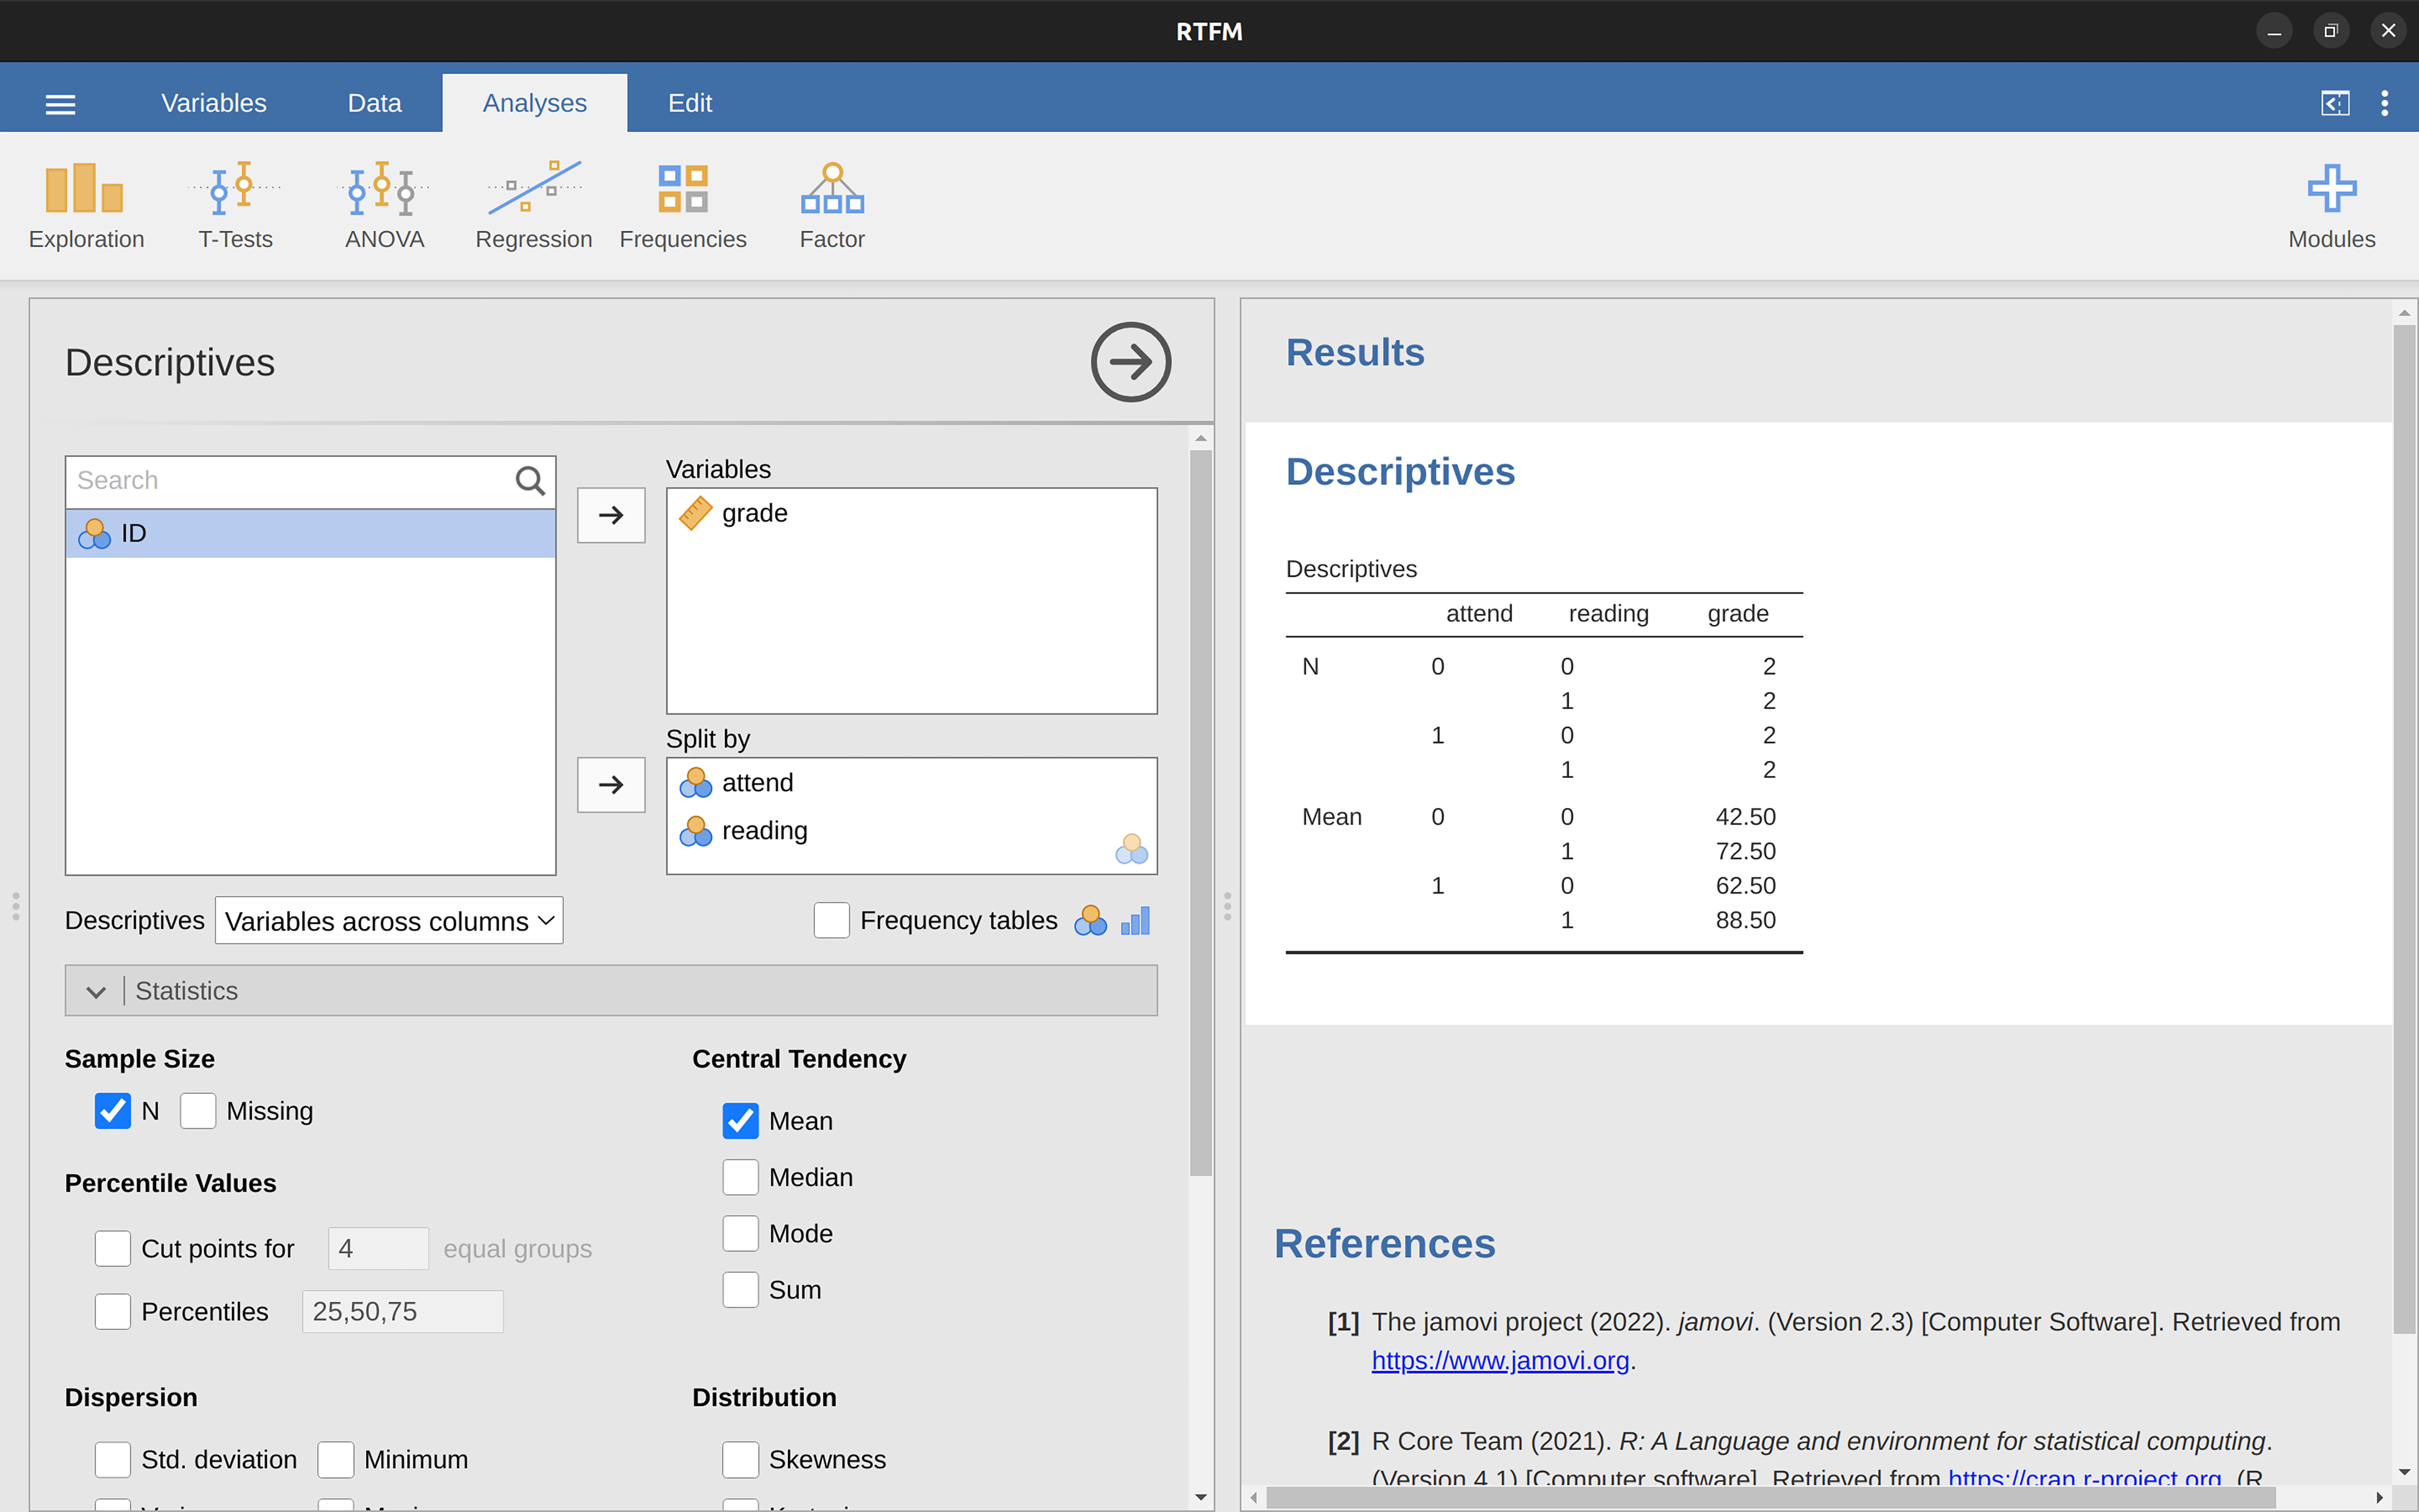
\includegraphics[width=1\textwidth,height=\textheight]{images/fig14-16.png} \hfill{}

\caption{\label{fig-fig14-16}jamovi descriptives for the \emph{rtfm.csv}
data set}

\end{figure}

\hypertarget{anova-with-binary-factors-as-a-regression-model}{%
\subsection{ANOVA with binary factors as a regression
model}\label{anova-with-binary-factors-as-a-regression-model}}

Okay, let's get back to talking about the mathematics. We now have our
data expressed in terms of three numeric variables: the continuous
variable \(Y\) and the two binary variables \(X_1\) and \(X_2\). What I
want you to recognise is that our \(2 \times 2\) factorial ANOVA is
exactly equivalent to the regression model:

\[Y_p=b_0+b_1 X_{1p} + b_2 X_{2p} + \epsilon_p\]

This is, of course, the exact same equation that I used earlier to
describe a two-predictor regression model! The only difference is that
\(X_1\) and \(X_2\) are now binary variables (i.e., values can only be 0
or 1), whereas in a regression analysis we expect that \(X_1\) and
\(X_2\) will be continuous. There's a couple of ways I could try to
convince you of this. One possibility would be to do a lengthy
mathematical exercise proving that the two are identical. However, I'm
going to go out on a limb and guess that most of the readership of this
book will find that annoying rather than helpful. Instead, I'll explain
the basic ideas and then rely on jamovi to show that ANOVA analyses and
regression analyses aren't just similar, they're identical for all
intents and purposes. Let's start by running this as an ANOVA. To do
this, we'll use the rtfm data set, and Figure~\ref{fig-fig14-17} shows
what we get when we run the analysis in jamovi.

\begin{figure}

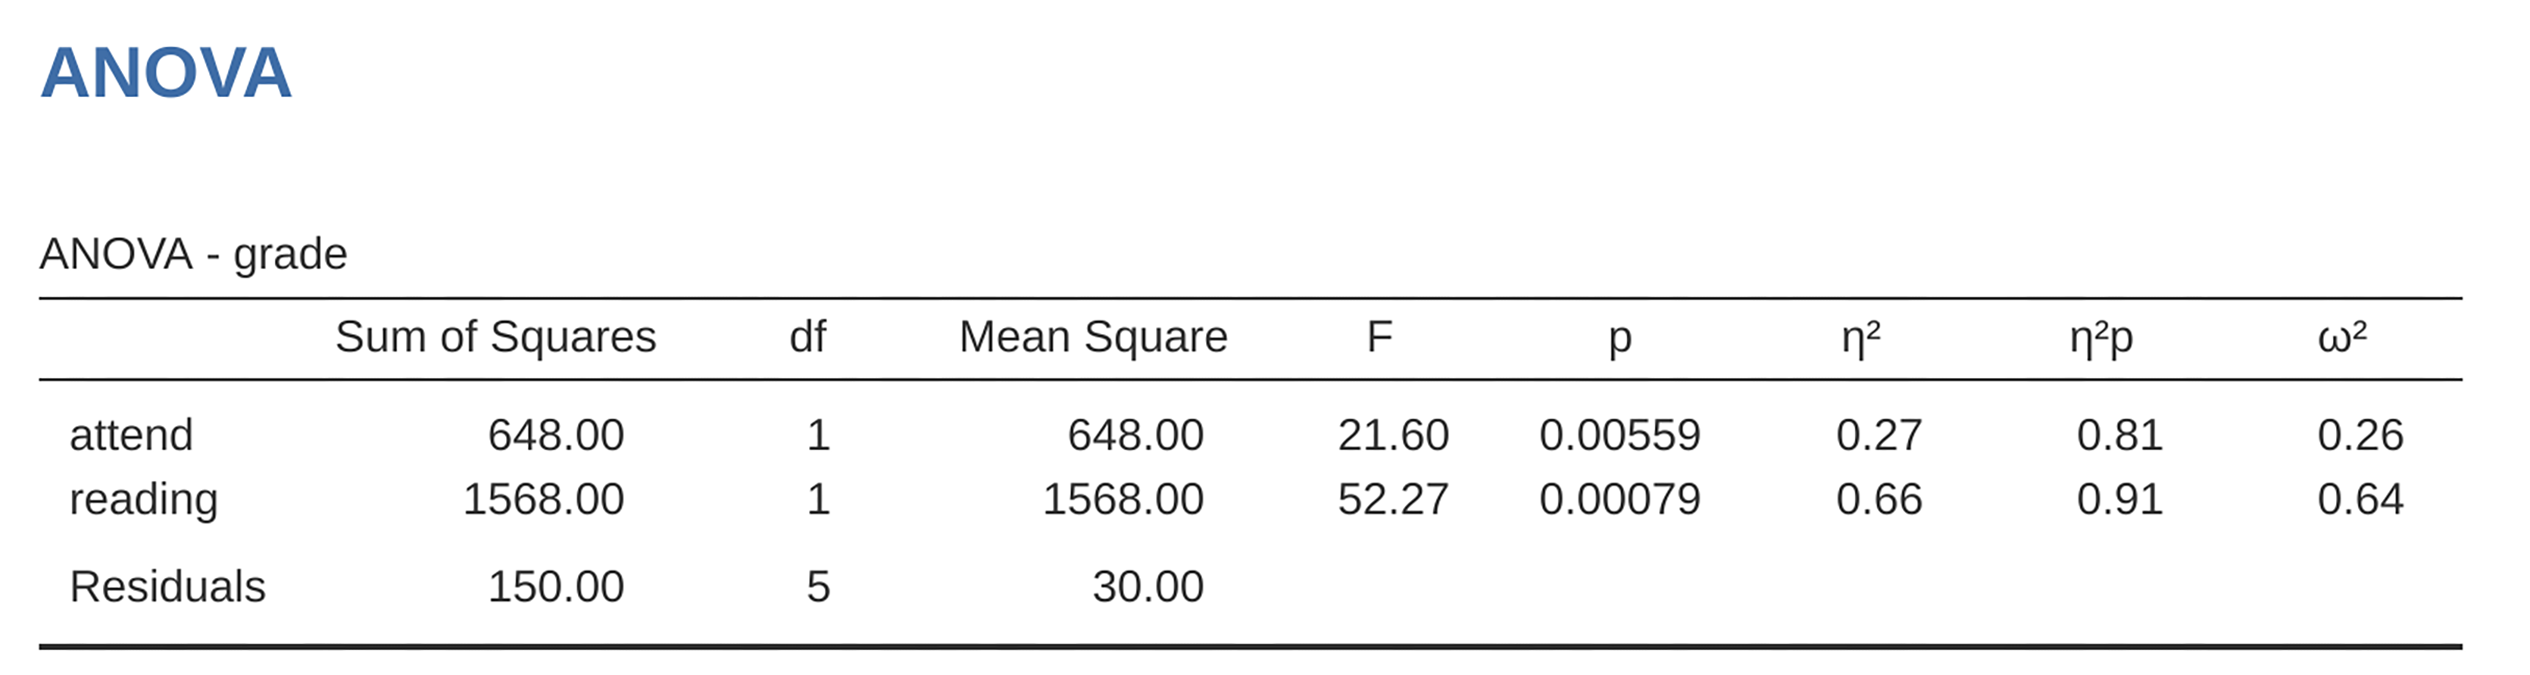
\includegraphics[width=1\textwidth,height=\textheight]{images/fig14-17.png} \hfill{}

\caption{\label{fig-fig14-17}ANOVA of the \emph{rtfm.csv} data set in
jamovi, without the interaction term}

\end{figure}

So, by reading the key numbers off the ANOVA table and the mean scores
that we presented earlier, we can see that the students obtained a
higher grade if they attended class (\(F_{1,5} = 21.6, p = .0056\)) and
if they read the textbook (\(F_{1,5} = 52.3, p = .0008\)). Let's make a
note of those \(p\)-values and those \(F\)-statistics.

Now let's think about the same analysis from a linear regression
perspective. In the \emph{rtfm.csv} data set, we have encoded attend and
reading as if they were numeric predictors. In this case, this is
perfectly acceptable. There really is a sense in which a student who
turns up to class (i.e.~attend = 1) has in fact done ``more attendance''
than a student who does not (i.e.~attend = 0). So it's not at all
unreasonable to include it as a predictor in a regression model. It's a
little unusual, because the predictor only takes on two possible values,
but it doesn't violate any of the assumptions of linear regression. And
it's easy to interpret. If the regression coefficient for attend is
greater than 0 it means that students that attend lectures get higher
grades. If it's less than zero then students attending lectures get
lower grades. The same is true for our reading variable.

Wait a second though. Why is this true? It's something that is
intuitively obvious to everyone who has taken a few stats classes and is
comfortable with the maths, but it isn't clear to everyone else at first
pass. To see why this is true, it helps to look closely at a few
specific students. Let's start by considering the 6th and 7th students
in our data set (i.e.~\(p = 6\) and \(p = 7\)). Neither one has read the
textbook, so in both cases we can set reading = 0. Or, to say the same
thing in our mathematical notation, we observe \(X_{2,6} = 0\) and
\(X_{2,7} = 0\). However, student number 7 did turn up to lectures
(i.e., attend = 1, \(X_{1,7} = 1\)) whereas student number 6 did not
(i.e., attend = 0, \(X_{1,6} = 0\)). Now let's look at what happens when
we insert these numbers into the general formula for our regression
line. For student number 6, the regression predicts that

\[
\begin{split}
\hat{Y}_6 & = b_0 + b_1 X_{1,6} + b_2 X_{2,6} \\
& = b_0 + (b_1 \times 0) + (b_2 \times 0) \\
& = b_0
\end{split}
\]

So we're expecting that this student will obtain a grade corresponding
to the value of the intercept term \(b_0\). What about student 7? This
time when we insert the numbers into the formula for the regression
line, we obtain the following

\[
\begin{split}
\hat{Y}_7 & = b_0 + b_1 X_{1,7} + b_2 X_{2,7} \\
& = b_0 + (b_1 \times 1) + (b_2 \times 0) \\
& = b_0 + b_1
\end{split}
\]

Because this student attended class, the predicted grade is equal to the
intercept term b0 plus the coefficient associated with the attend
variable, \(b_1\). So, if \(b_1\) is greater than zero, we're expecting
that the students who turn up to lectures will get higher grades than
those students who don't. If this coefficient is negative we're
expecting the opposite: students who turn up at class end up performing
much worse. In fact, we can push this a little bit further. What about
student number 1, who turned up to class (\(X_{1,1} = 1\)) and read the
textbook (\(X_{2,1} = 1\))? If we plug these numbers into the regression
we get

\[
\begin{split}
\hat{Y}_1 & = b_0 + b_1 X_{1,1} + b_2 X_{2,1} \\
& = b_0 + (b_1 \times 1) + (b_2 \times 1) \\
& = b_0 + b_1 + b_2
\end{split}
\]

So if we assume that attending class helps you get a good grade (i.e.,
\(b_1 > 0\)) and if we assume that reading the textbook also helps you
get a good grade (i.e., \(b_2 > 0\)), then our expectation is that
student 1 will get a grade that that is higher than student 6 and
student 7.

And at this point you won't be at all suprised to learn that the
regression model predicts that student 3, who read the book but didn't
attend lectures, will obtain a grade of \(b_{2} + b_{0}\). I won't bore
you with yet another regression formula. Instead, what I'll do is show
you is Table~\ref{tbl-tab14-9} with the \emph{expected grades}.

\hypertarget{tbl-tab14-9}{}
 
  \providecommand{\huxb}[2]{\arrayrulecolor[RGB]{#1}\global\arrayrulewidth=#2pt}
  \providecommand{\huxvb}[2]{\color[RGB]{#1}\vrule width #2pt}
  \providecommand{\huxtpad}[1]{\rule{0pt}{#1}}
  \providecommand{\huxbpad}[1]{\rule[-#1]{0pt}{#1}}

\begin{table}[ht]
\caption{\label{tbl-tab14-9}Expected grades from the regression model }\tabularnewline

\begin{centerbox}
\begin{threeparttable}
\setlength{\tabcolsep}{0pt}
\begin{tabularx}{0.9\textwidth}{p{0.225\textwidth} p{0.225\textwidth} p{0.225\textwidth} p{0.225\textwidth}}


\hhline{>{\huxb{0, 0, 0}{0.4}}->{\huxb{0, 0, 0}{0.4}}->{\huxb{0, 0, 0}{0.4}}->{\huxb{0, 0, 0}{0.4}}-}
\arrayrulecolor{black}

\multicolumn{1}{!{\huxvb{0, 0, 0}{0}}p{0.225\textwidth}!{\huxvb{0, 0, 0}{0}}}{\hspace{0pt}\parbox[b]{0.225\textwidth-0pt-12pt}{\huxtpad{2pt + 1em}\centering \textbf{}\huxbpad{2pt}}} &
\multicolumn{1}{p{0.225\textwidth}!{\huxvb{0, 0, 0}{0}}}{\hspace{12pt}\parbox[b]{0.225\textwidth-12pt-12pt}{\huxtpad{2pt + 1em}\centering \textbf{}\huxbpad{2pt}}} &
\multicolumn{1}{p{0.225\textwidth}!{\huxvb{0, 0, 0}{0}}}{\hspace{12pt}\parbox[b]{0.225\textwidth-12pt-12pt}{\huxtpad{2pt + 1em}\centering \textbf{read textbook}\huxbpad{2pt}}} &
\multicolumn{1}{p{0.225\textwidth}!{\huxvb{0, 0, 0}{0}}}{\hspace{12pt}\parbox[b]{0.225\textwidth-12pt-0pt}{\huxtpad{2pt + 1em}\centering \textbf{}\huxbpad{2pt}}} \tabularnewline[-0.5pt]


\hhline{>{\huxb{0, 0, 0}{0.4}}->{\huxb{0, 0, 0}{0.4}}->{\huxb{0, 0, 0}{0.4}}->{\huxb{0, 0, 0}{0.4}}-}
\arrayrulecolor{black}

\multicolumn{1}{!{\huxvb{0, 0, 0}{0}}p{0.225\textwidth}!{\huxvb{0, 0, 0}{0}}}{\hspace{0pt}\parbox[b]{0.225\textwidth-0pt-12pt}{\huxtpad{2pt + 1em}\centering \huxbpad{2pt}}} &
\multicolumn{1}{p{0.225\textwidth}!{\huxvb{0, 0, 0}{0}}}{\hspace{12pt}\parbox[b]{0.225\textwidth-12pt-12pt}{\huxtpad{2pt + 1em}\centering \huxbpad{2pt}}} &
\multicolumn{1}{p{0.225\textwidth}!{\huxvb{0, 0, 0}{0}}}{\hspace{12pt}\parbox[b]{0.225\textwidth-12pt-12pt}{\huxtpad{2pt + 1em}\centering no\huxbpad{2pt}}} &
\multicolumn{1}{p{0.225\textwidth}!{\huxvb{0, 0, 0}{0}}}{\hspace{12pt}\parbox[b]{0.225\textwidth-12pt-0pt}{\huxtpad{2pt + 1em}\centering yes\huxbpad{2pt}}} \tabularnewline[-0.5pt]


\hhline{}
\arrayrulecolor{black}

\multicolumn{1}{!{\huxvb{0, 0, 0}{0}}p{0.225\textwidth}!{\huxvb{0, 0, 0}{0}}}{\hspace{0pt}\parbox[b]{0.225\textwidth-0pt-12pt}{\huxtpad{2pt + 1em}\centering attended?\huxbpad{2pt}}} &
\multicolumn{1}{p{0.225\textwidth}!{\huxvb{0, 0, 0}{0}}}{\hspace{12pt}\parbox[b]{0.225\textwidth-12pt-12pt}{\huxtpad{2pt + 1em}\centering no\huxbpad{2pt}}} &
\multicolumn{1}{p{0.225\textwidth}!{\huxvb{0, 0, 0}{0}}}{\hspace{12pt}\parbox[b]{0.225\textwidth-12pt-12pt}{\huxtpad{2pt + 1em}\centering \( \beta_0 \)\huxbpad{2pt}}} &
\multicolumn{1}{p{0.225\textwidth}!{\huxvb{0, 0, 0}{0}}}{\hspace{12pt}\parbox[b]{0.225\textwidth-12pt-0pt}{\huxtpad{2pt + 1em}\centering \( \beta_0 + \beta_2 \)\huxbpad{2pt}}} \tabularnewline[-0.5pt]


\hhline{}
\arrayrulecolor{black}

\multicolumn{1}{!{\huxvb{0, 0, 0}{0}}p{0.225\textwidth}!{\huxvb{0, 0, 0}{0}}}{\hspace{0pt}\parbox[b]{0.225\textwidth-0pt-12pt}{\huxtpad{2pt + 1em}\centering \huxbpad{2pt}}} &
\multicolumn{1}{p{0.225\textwidth}!{\huxvb{0, 0, 0}{0}}}{\hspace{12pt}\parbox[b]{0.225\textwidth-12pt-12pt}{\huxtpad{2pt + 1em}\centering yes\huxbpad{2pt}}} &
\multicolumn{1}{p{0.225\textwidth}!{\huxvb{0, 0, 0}{0}}}{\hspace{12pt}\parbox[b]{0.225\textwidth-12pt-12pt}{\huxtpad{2pt + 1em}\centering \( \beta_0 + \beta_1 \)\huxbpad{2pt}}} &
\multicolumn{1}{p{0.225\textwidth}!{\huxvb{0, 0, 0}{0}}}{\hspace{12pt}\parbox[b]{0.225\textwidth-12pt-0pt}{\huxtpad{2pt + 1em}\centering \( \beta_0 + \beta_1 + \beta_2 \)\huxbpad{2pt}}} \tabularnewline[-0.5pt]


\hhline{>{\huxb{0, 0, 0}{0.4}}->{\huxb{0, 0, 0}{0.4}}->{\huxb{0, 0, 0}{0.4}}->{\huxb{0, 0, 0}{0.4}}-}
\arrayrulecolor{black}
\end{tabularx} 

\end{threeparttable}\par\end{centerbox}

\end{table}
 

As you can see, the intercept term \(b_0\) acts like a kind of
``baseline'' grade that you would expect from those students who don't
take the time to attend class or read the textbook. Similarly, \(b_1\)
represents the boost that you're expected to get if you come to class,
and \(b_2\) represents the boost that comes from reading the textbook.
In fact, if this were an ANOVA you might very well want to characterise
\(b_1\) as the main effect of attendance, and \(b_2\) as the main effect
of reading! In fact, for a simple \(2 \times 2\) ANOVA that's exactly
how it plays out.

Okay, now that we're really starting to see why ANOVA and regression are
basically the same thing, let's actually run our regression using the
rtfm data and the jamovi regression analysis to convince ourselves that
this is really true. Running the regression in the usual way gives the
results shown in Figure~\ref{fig-fig14-18}.

\begin{figure}

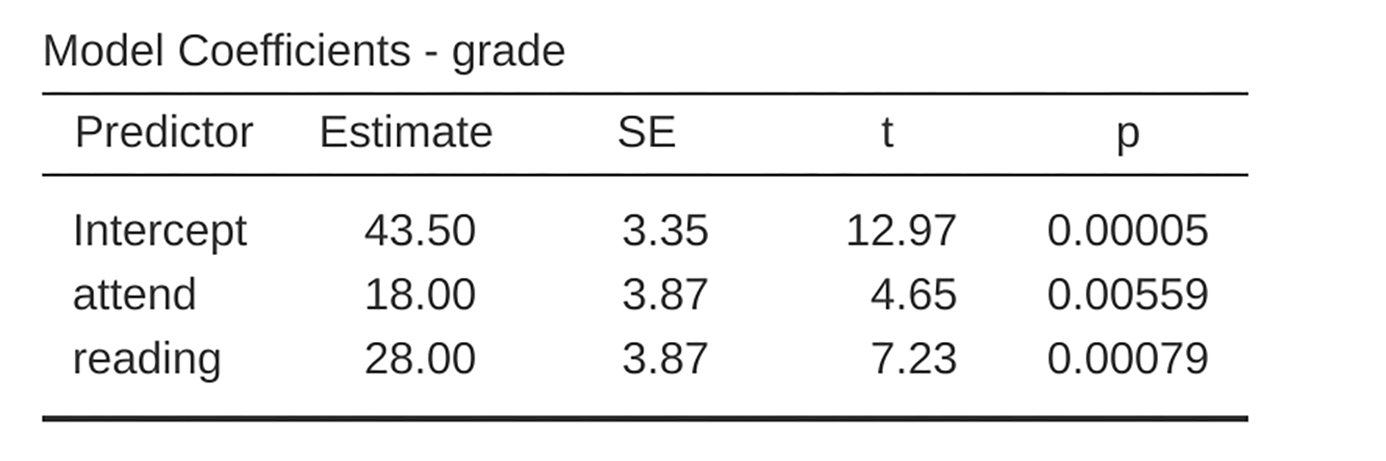
\includegraphics[width=1\textwidth,height=\textheight]{images/fig14-18.png} \hfill{}

\caption{\label{fig-fig14-18}Regression analysis of the \emph{rtfm.csv}
data set in jamovi, without the interaction term}

\end{figure}

There's a few interesting things to note here. First, notice that the
intercept term is 43.5 which is close to the ``group'' mean of 42.5
observed for those two students who didn't read the text or attend
class. Second, notice that we have the regression coefficient of
\(b_1 = 18.0\) for the attendance variable, suggesting that those
students that attended class scored 18\% higher than those who didn't.
So our expectation would be that those students who turned up to class
but didn't read the textbook would obtain a grade of \(b_0 + b_1\),
which is equal to \(43.5 + 18.0 = 61.5\). You can verify for yourself
that the same thing happens when we look at the students that read the
textbook.

Actually, we can push a little further in establishing the equivalence
of our ANOVA and our regression. Look at the \(p\)-values associated
with the attend variable and the reading variable in the regression
output. They're identical to the ones we encountered earlier when
running the ANOVA. This might seem a little surprising, since the test
used when running our regression model calculates a \(t\)-statistic and
the ANOVA calculates an \(F\)-statistic. However, if you can remember
all the way back to \textbf{?@sec-Introduction-to-probability}, I
mentioned that there's a relationship between the \(t\)-distribution and
the \(F\)-distribution. If you have some quantity that is distributed
according to a \(t\)-distribution with \(k\) degrees of freedom and you
square it, then this new squared quantity follows an \(F\)-distribution
whose degrees of freedom are 1 and \(k\). We can check this with respect
to the \(t\)-statistics in our regression model. For the attend variable
we get a \(t\)-value of 4.65. If we square this number we end up with
21.6, which matches the corresponding \(F\)-statistic in our ANOVA.

Finally, one last thing you should know. Because jamovi understands the
fact that ANOVA and regression are both examples of linear models, it
lets you extract the classic ANOVA table from your regression model
using the `Linear Regression' - `Model Coefficients' - `Omnibus Test' -
`ANOVA Test', and this will give you the table shown in
Figure~\ref{fig-fig14-19}.

\begin{figure}

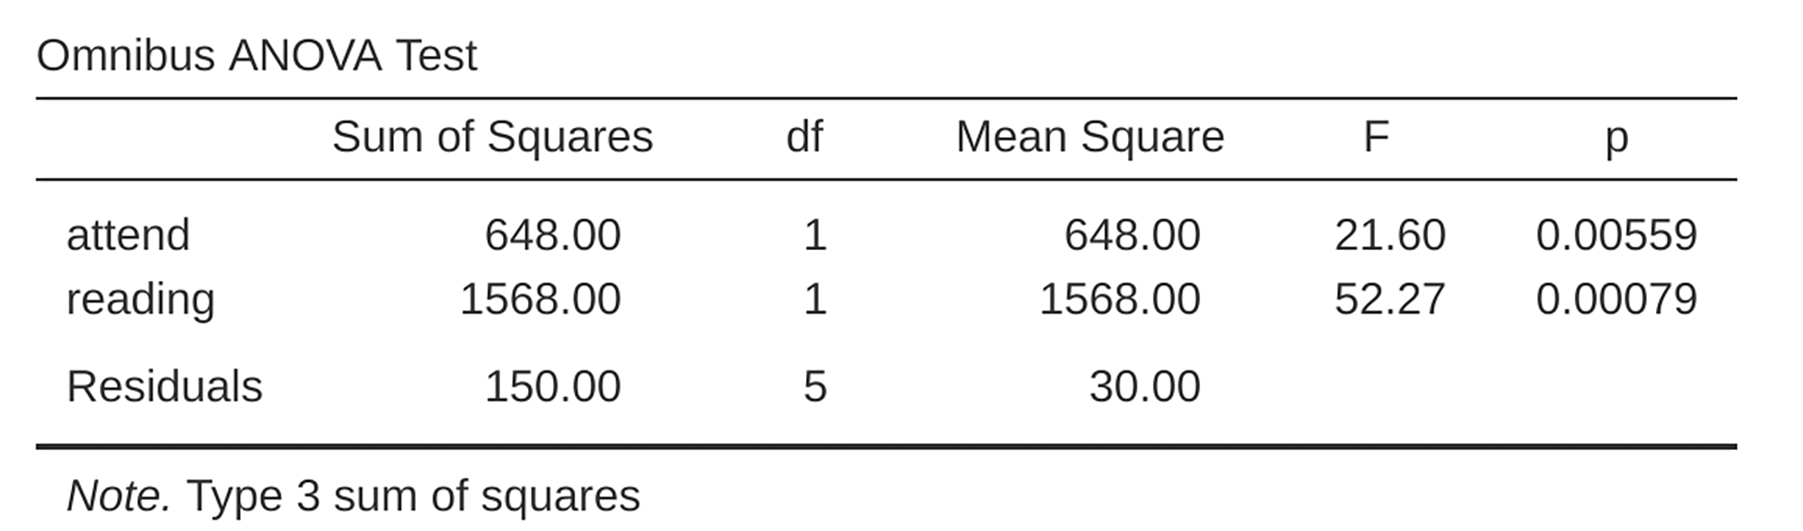
\includegraphics[width=1\textwidth,height=\textheight]{images/fig14-19.png} \hfill{}

\caption{\label{fig-fig14-19}Omnibus ANOVA Test results from the jamovi
regression analysis}

\end{figure}

\hypertarget{how-to-encode-non-binary-factors-as-contrasts}{%
\subsection{How to encode non binary factors as
contrasts}\label{how-to-encode-non-binary-factors-as-contrasts}}

At this point, I've shown you how we can view a \(2 \times 2\) ANOVA
into a linear model. And it's pretty easy to see how this generalises to
a \(2 \times 2 \times 2\) ANOVA or a \(2 \times 2 \times 2 \times 2\)
ANOVA. It's the same thing, really. You just add a new binary variable
for each of your factors. Where it begins to get trickier is when we
consider factors that have more than two levels. Consider, for instance,
the \(3 \times 2\) ANOVA that we ran earlier in this chapter using the
\emph{clinicaltrial.csv} data. How can we convert the three-level drug
factor into a numerical form that is appropriate for a regression?

The answer to this question is pretty simple, actually. All we have to
do is realise that a three-level factor can be redescribed as two binary
variables. Suppose, for instance, I were to create a new binary variable
called druganxifree. Whenever the drug variable is equal to ``anxifree''
we set druganxifree = 1. Otherwise, we set druganxifree = 0. This
variable sets up a \textbf{contrast}, in this case between anxifree and
the other two drugs. By itself, of course, the druganxifree contrast
isn't enough to fully capture all of the information in our drug
variable. We need a second contrast, one that allows us to distinguish
between joyzepam and the placebo. To do this, we can create a second
binary contrast, called drugjoyzepam, which equals 1 if the drug is
joyzepam and 0 if it is not. Taken together, these two contrasts allows
us to perfectly discriminate between all three possible drugs.
Table~\ref{tbl-tab14-10} illustrates this.

\hypertarget{tbl-tab14-10}{}
 
  \providecommand{\huxb}[2]{\arrayrulecolor[RGB]{#1}\global\arrayrulewidth=#2pt}
  \providecommand{\huxvb}[2]{\color[RGB]{#1}\vrule width #2pt}
  \providecommand{\huxtpad}[1]{\rule{0pt}{#1}}
  \providecommand{\huxbpad}[1]{\rule[-#1]{0pt}{#1}}

\begin{table}[ht]
\caption{\label{tbl-tab14-10}Binary contrasts to discriminate between all three possible drugs }\tabularnewline

\begin{centerbox}
\begin{threeparttable}
\setlength{\tabcolsep}{0pt}
\begin{tabularx}{0.9\textwidth}{p{0.3\textwidth} p{0.3\textwidth} p{0.3\textwidth}}


\hhline{>{\huxb{0, 0, 0}{0.4}}->{\huxb{0, 0, 0}{0.4}}->{\huxb{0, 0, 0}{0.4}}-}
\arrayrulecolor{black}

\multicolumn{1}{!{\huxvb{0, 0, 0}{0}}p{0.3\textwidth}!{\huxvb{0, 0, 0}{0}}}{\hspace{0pt}\parbox[b]{0.3\textwidth-0pt-12pt}{\huxtpad{2pt + 1em}\centering \textbf{drug}\huxbpad{2pt}}} &
\multicolumn{1}{p{0.3\textwidth}!{\huxvb{0, 0, 0}{0}}}{\hspace{12pt}\parbox[b]{0.3\textwidth-12pt-12pt}{\huxtpad{2pt + 1em}\centering \textbf{druganxifree}\huxbpad{2pt}}} &
\multicolumn{1}{p{0.3\textwidth}!{\huxvb{0, 0, 0}{0}}}{\hspace{12pt}\parbox[b]{0.3\textwidth-12pt-0pt}{\huxtpad{2pt + 1em}\centering \textbf{drugjoyzepam}\huxbpad{2pt}}} \tabularnewline[-0.5pt]


\hhline{>{\huxb{0, 0, 0}{0.4}}->{\huxb{0, 0, 0}{0.4}}->{\huxb{0, 0, 0}{0.4}}-}
\arrayrulecolor{black}

\multicolumn{1}{!{\huxvb{0, 0, 0}{0}}p{0.3\textwidth}!{\huxvb{0, 0, 0}{0}}}{\hspace{0pt}\parbox[b]{0.3\textwidth-0pt-12pt}{\huxtpad{2pt + 1em}\centering ``placebo"\huxbpad{2pt}}} &
\multicolumn{1}{p{0.3\textwidth}!{\huxvb{0, 0, 0}{0}}}{\hspace{12pt}\parbox[b]{0.3\textwidth-12pt-12pt}{\huxtpad{2pt + 1em}\centering 0\huxbpad{2pt}}} &
\multicolumn{1}{p{0.3\textwidth}!{\huxvb{0, 0, 0}{0}}}{\hspace{12pt}\parbox[b]{0.3\textwidth-12pt-0pt}{\huxtpad{2pt + 1em}\centering 0\huxbpad{2pt}}} \tabularnewline[-0.5pt]


\hhline{}
\arrayrulecolor{black}

\multicolumn{1}{!{\huxvb{0, 0, 0}{0}}p{0.3\textwidth}!{\huxvb{0, 0, 0}{0}}}{\hspace{0pt}\parbox[b]{0.3\textwidth-0pt-12pt}{\huxtpad{2pt + 1em}\centering ``anxifree"\huxbpad{2pt}}} &
\multicolumn{1}{p{0.3\textwidth}!{\huxvb{0, 0, 0}{0}}}{\hspace{12pt}\parbox[b]{0.3\textwidth-12pt-12pt}{\huxtpad{2pt + 1em}\centering 1\huxbpad{2pt}}} &
\multicolumn{1}{p{0.3\textwidth}!{\huxvb{0, 0, 0}{0}}}{\hspace{12pt}\parbox[b]{0.3\textwidth-12pt-0pt}{\huxtpad{2pt + 1em}\centering 0\huxbpad{2pt}}} \tabularnewline[-0.5pt]


\hhline{}
\arrayrulecolor{black}

\multicolumn{1}{!{\huxvb{0, 0, 0}{0}}p{0.3\textwidth}!{\huxvb{0, 0, 0}{0}}}{\hspace{0pt}\parbox[b]{0.3\textwidth-0pt-12pt}{\huxtpad{2pt + 1em}\centering ``joyzepam"\huxbpad{2pt}}} &
\multicolumn{1}{p{0.3\textwidth}!{\huxvb{0, 0, 0}{0}}}{\hspace{12pt}\parbox[b]{0.3\textwidth-12pt-12pt}{\huxtpad{2pt + 1em}\centering 0\huxbpad{2pt}}} &
\multicolumn{1}{p{0.3\textwidth}!{\huxvb{0, 0, 0}{0}}}{\hspace{12pt}\parbox[b]{0.3\textwidth-12pt-0pt}{\huxtpad{2pt + 1em}\centering 1\huxbpad{2pt}}} \tabularnewline[-0.5pt]


\hhline{>{\huxb{0, 0, 0}{0.4}}->{\huxb{0, 0, 0}{0.4}}->{\huxb{0, 0, 0}{0.4}}-}
\arrayrulecolor{black}
\end{tabularx} 

\end{threeparttable}\par\end{centerbox}

\end{table}
 

If the drug administered to a patient is a placebo then both of the two
contrast variables will equal 0. If the drug is Anxifree then the
druganxifree variable will equal 1, and drugjoyzepam will be 0. The
reverse is true for Joyzepam: drugjoyzepam is 1 and druganxifree is 0.

Creating contrast variables is not too difficult to do using the jamovi
compute new variable command. For example, to create the druganxifree
variable, write this logical expression in the compute new variable
formula box:

\begin{quote}
IF(drug == `anxifree', 1, 0)
\end{quote}

Similarly, to create the new variable drugjoyzepam use this logical
expression:

\begin{quote}
IF(drug == `joyzepam', 1, 0)
\end{quote}

Likewise for CBTtherapy:

\begin{quote}
IF(therapy == `CBT', 1, 0)
\end{quote}

You can see these new variables, and the corresponding logical
expressions, in the jamovi data file \emph{clinicaltrial2.omv} .

We have now recoded our three-level factor in terms of two binary
variables, and we've already seen that ANOVA and regression behave the
same way for binary variables. However, there are some additional
complexities that arise in this case, which we'll discuss in the next
section.

\hypertarget{the-equivalence-between-anova-and-regression-for-non-binary-factors}{%
\subsection{The equivalence between ANOVA and regression for non-binary
factors}\label{the-equivalence-between-anova-and-regression-for-non-binary-factors}}

Now we have two different versions of the same data set. Our original
data in which the drug variable from the \emph{clinicaltrial.csv} file
is expressed as a single three-level factor, and the expanded data
\emph{clinicaltrial2.omv} in which it is expanded into two binary
contrasts. Once again, the thing that we want to demonstrate is that our
original \(3 \times 2\) factorial ANOVA is equivalent to a regression
model applied to the contrast variables. Let's start by re-running the
ANOVA, with results shown in Figure~\ref{fig-fig14-20}.

\begin{figure}

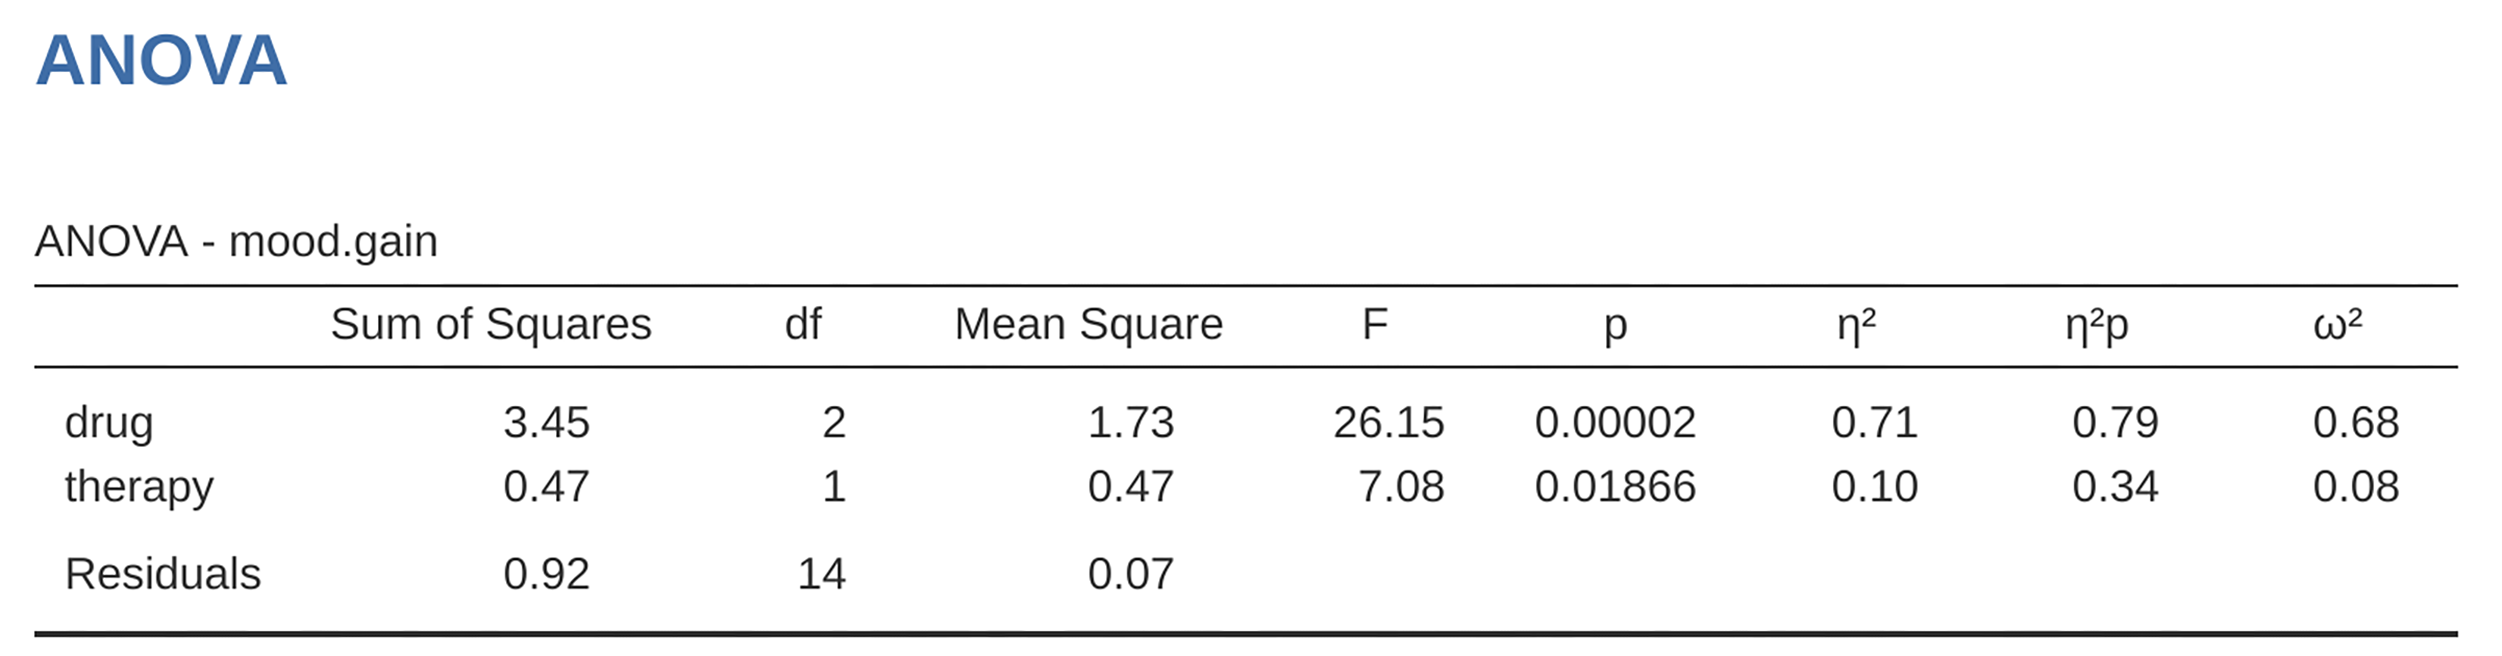
\includegraphics[width=1\textwidth,height=\textheight]{images/fig14-20.png} \hfill{}

\caption{\label{fig-fig14-20}jamovi ANOVA results, without interaction
component}

\end{figure}

Obviously, there are no surprises here. That's the exact same ANOVA that
we ran earlier. Next, let's run a regression using druganxifree,
drugjoyzepam and CBTtherapy as the predictors. The results are shown in
Figure~\ref{fig-fig14-21}.

\begin{figure}

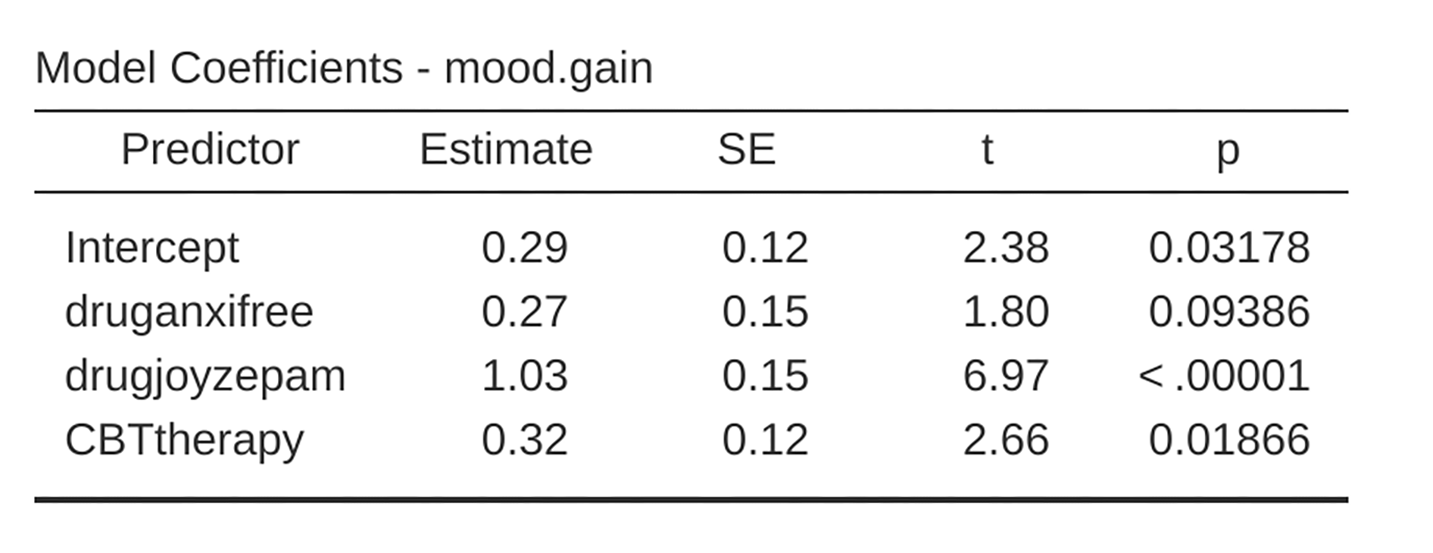
\includegraphics[width=1\textwidth,height=\textheight]{images/fig14-21.png} \hfill{}

\caption{\label{fig-fig14-21}jamovi regression results, with contrast
variables druganxifree and drugjoyzepam}

\end{figure}

Hmm. This isn't the same output that we got last time. Not surprisingly,
the regression output prints out the results for each of the three
predictors separately, just like it did every other time we conducted a
regression analysis. On the one hand we can see that the \(p\)-value for
the CBTtherapy variable is exactly the same as the one for the therapy
factor in our original ANOVA, so we can be reassured that the regression
model is doing the same thing as the ANOVA did. On the other hand, this
regression model is testing the druganxifree contrast and the
drugjoyzepam contrast \emph{separately}, as if they were two completely
unrelated variables. It's not surprising of course, because the poor
regression analysis has no way of knowing that drugjoyzepam and
druganxifree are actually the two different contrasts that we used to
encode our three-level drug factor. As far as it knows, drugjoyzepam and
druganxifree are no more related to one another than drugjoyzepam and
therapyCBT. However, you and I know better. At this stage we're not at
all interested in determining whether these two contrasts are
individually significant. We just want to know if there's an ``overall''
effect of drug. That is, what we want jamovi to do is to run some kind
of ``model comparison'' test, one in which the two ``drug related''
contrasts are lumped together for the purpose of the test. Sound
familiar? All we need to do is specify our null model, which in this
case would include the CBTtherapy predictor, and omit both of the
drug-related variables, as in Figure~\ref{fig-fig14-22}.

\begin{figure}

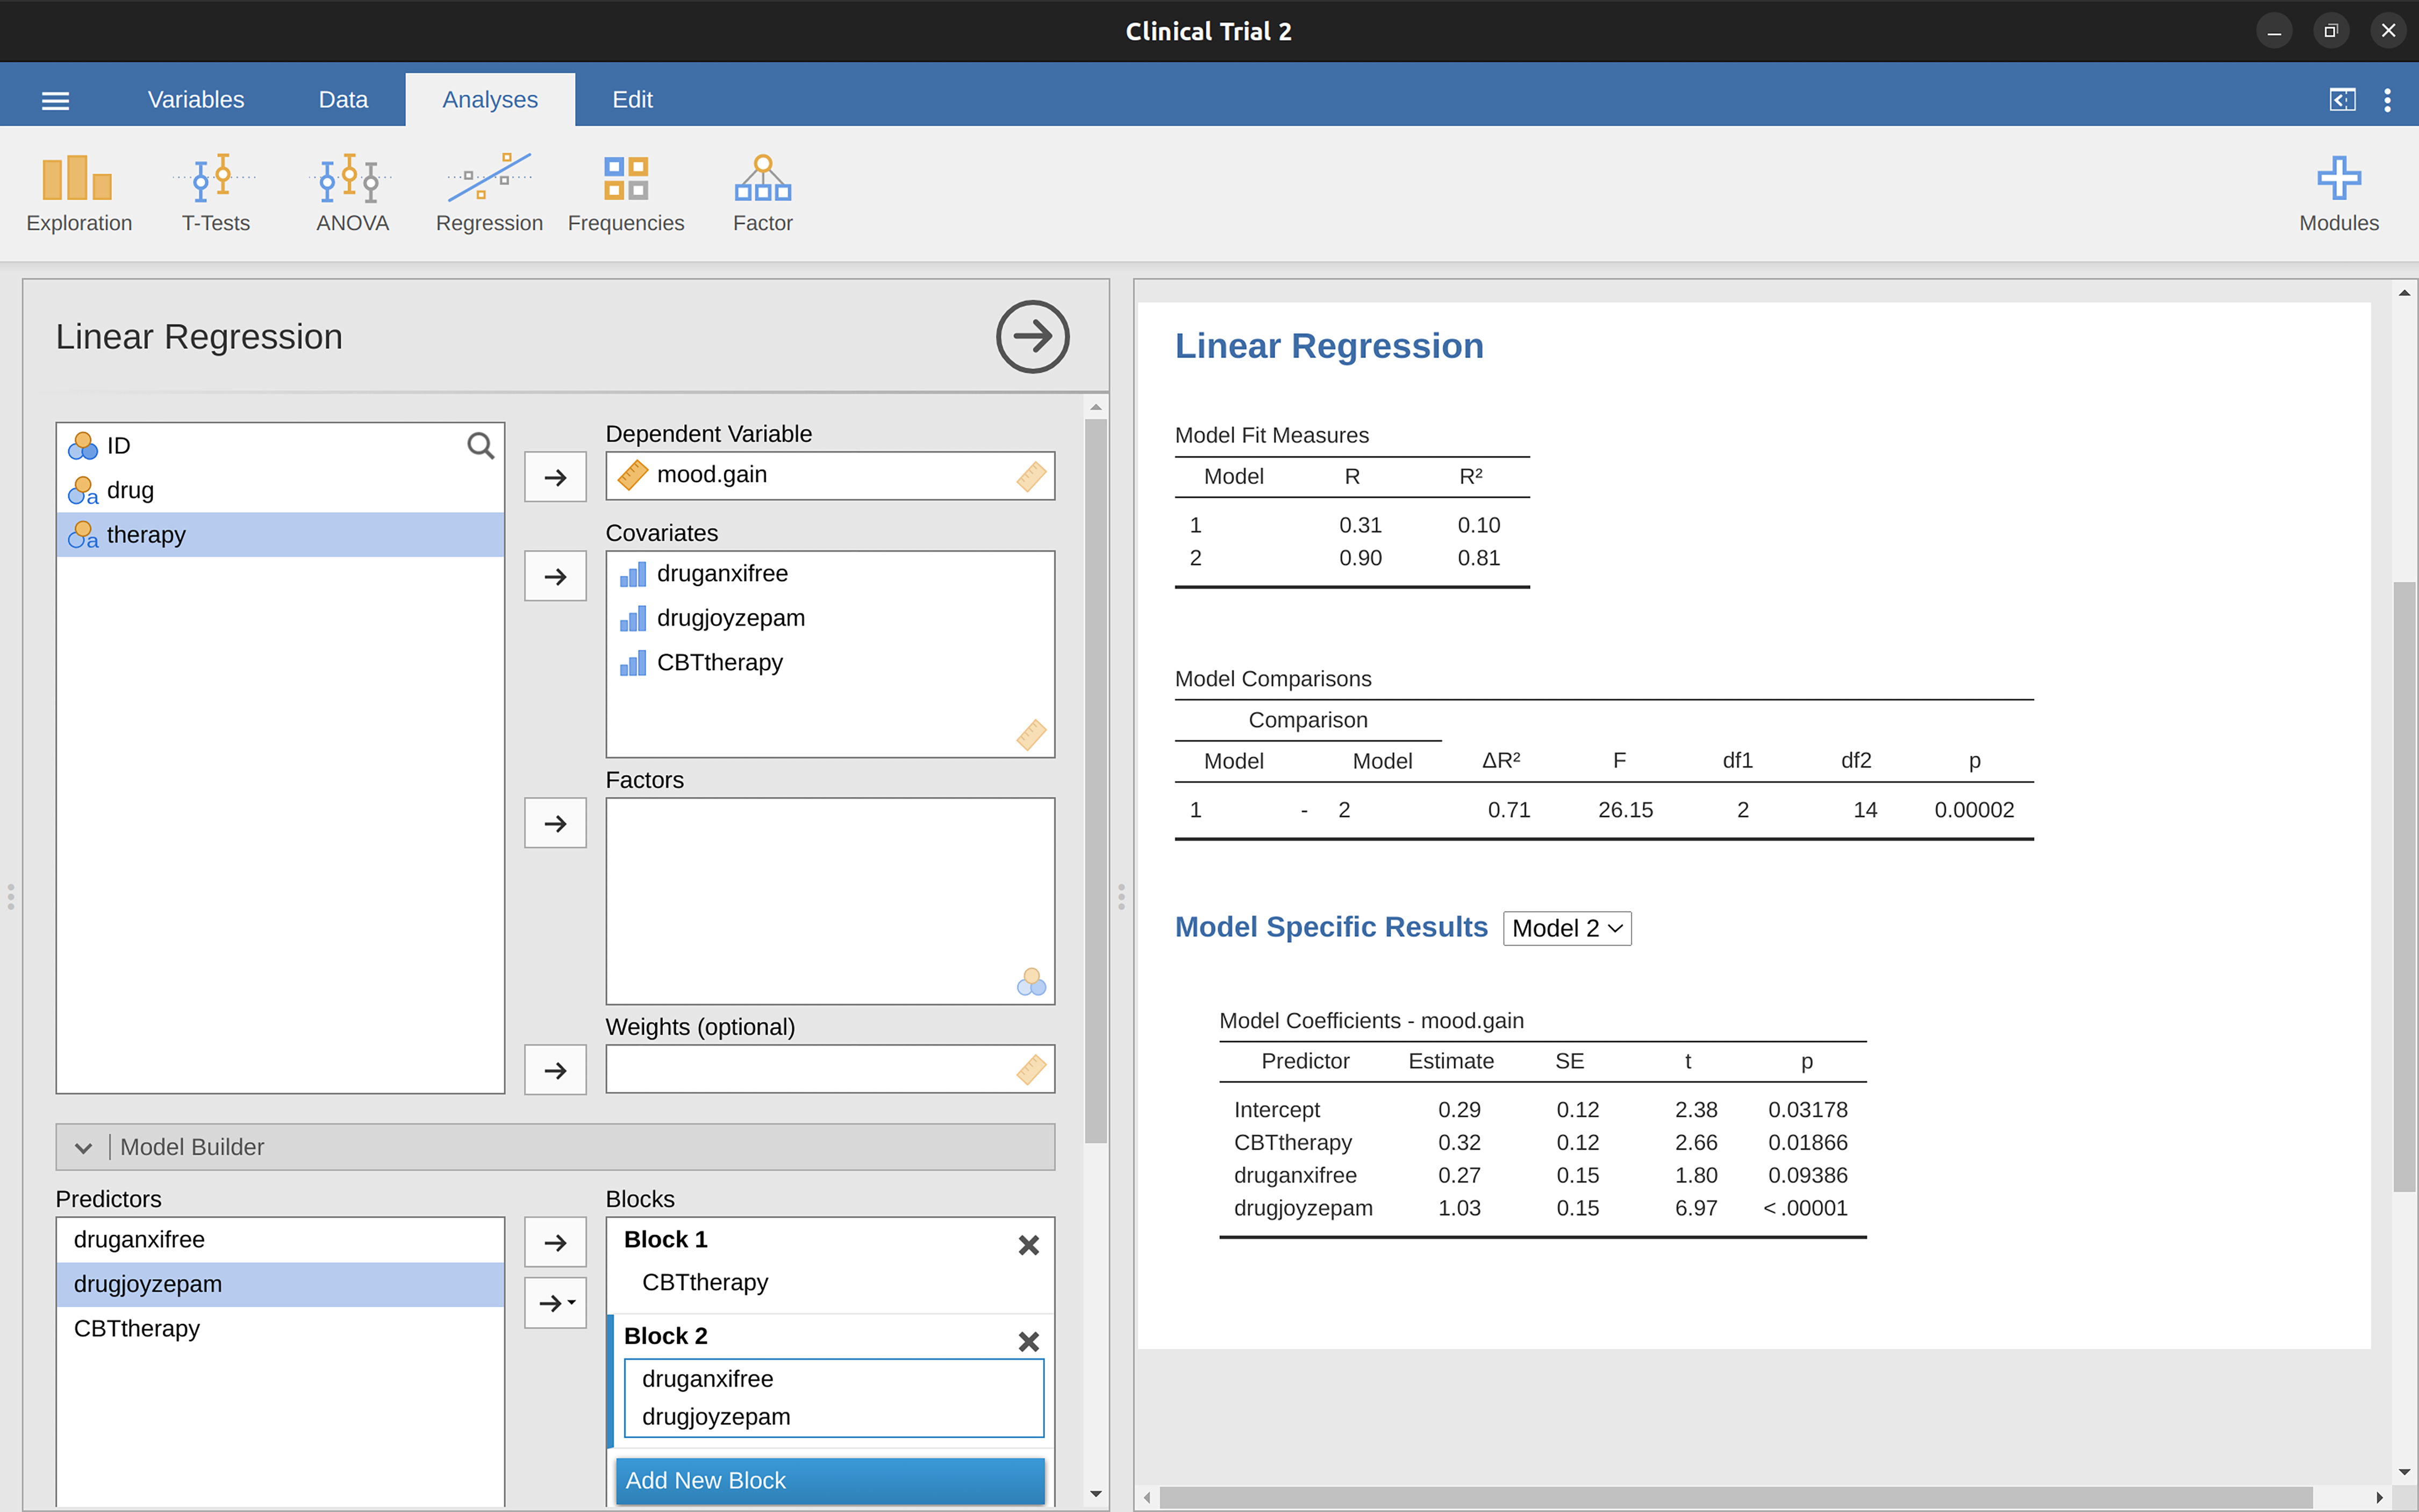
\includegraphics[width=1\textwidth,height=\textheight]{images/fig14-22.png} \hfill{}

\caption{\label{fig-fig14-22}Model comparison in jamovi regression, null
model 1 vs.~contrasts model 2}

\end{figure}

Ah, that's better. Our \(F\)-statistic is 26.15, the degrees of freedom
are 2 and 14, and the \(p\)-value is 0.00002. The numbers are identical
to the ones we obtained for the main effect of drug in our original
ANOVA. Once again we see that ANOVA and regression are essentially the
same. They are both linear models, and the underlying statistical
machinery for ANOVA is identical to the machinery used in regression.
The importance of this fact should not be understated. Throughout the
rest of this chapter we're going to rely heavily on this idea.

Although we went through all the faff of computing new variables in
jamovi for the contrasts druganxifree and drugjoyzepam, just to show
that ANOVA and regression are essentially the same, in the jamovi linear
regression analysis there is actually a nifty shortcut to get these
contrasts, see Figure~\ref{fig-fig14-23}. What jamovi is doing here is
allowing you to enter the predictor variables that are factors as, wait
for it\ldots factors! Smart, eh. You can also specify which group to use
as the reference level, via the `Reference Levels' option. We've changed
this to `placebo' and `no.therapy', respectively, because this makes
most sense.

\begin{figure}

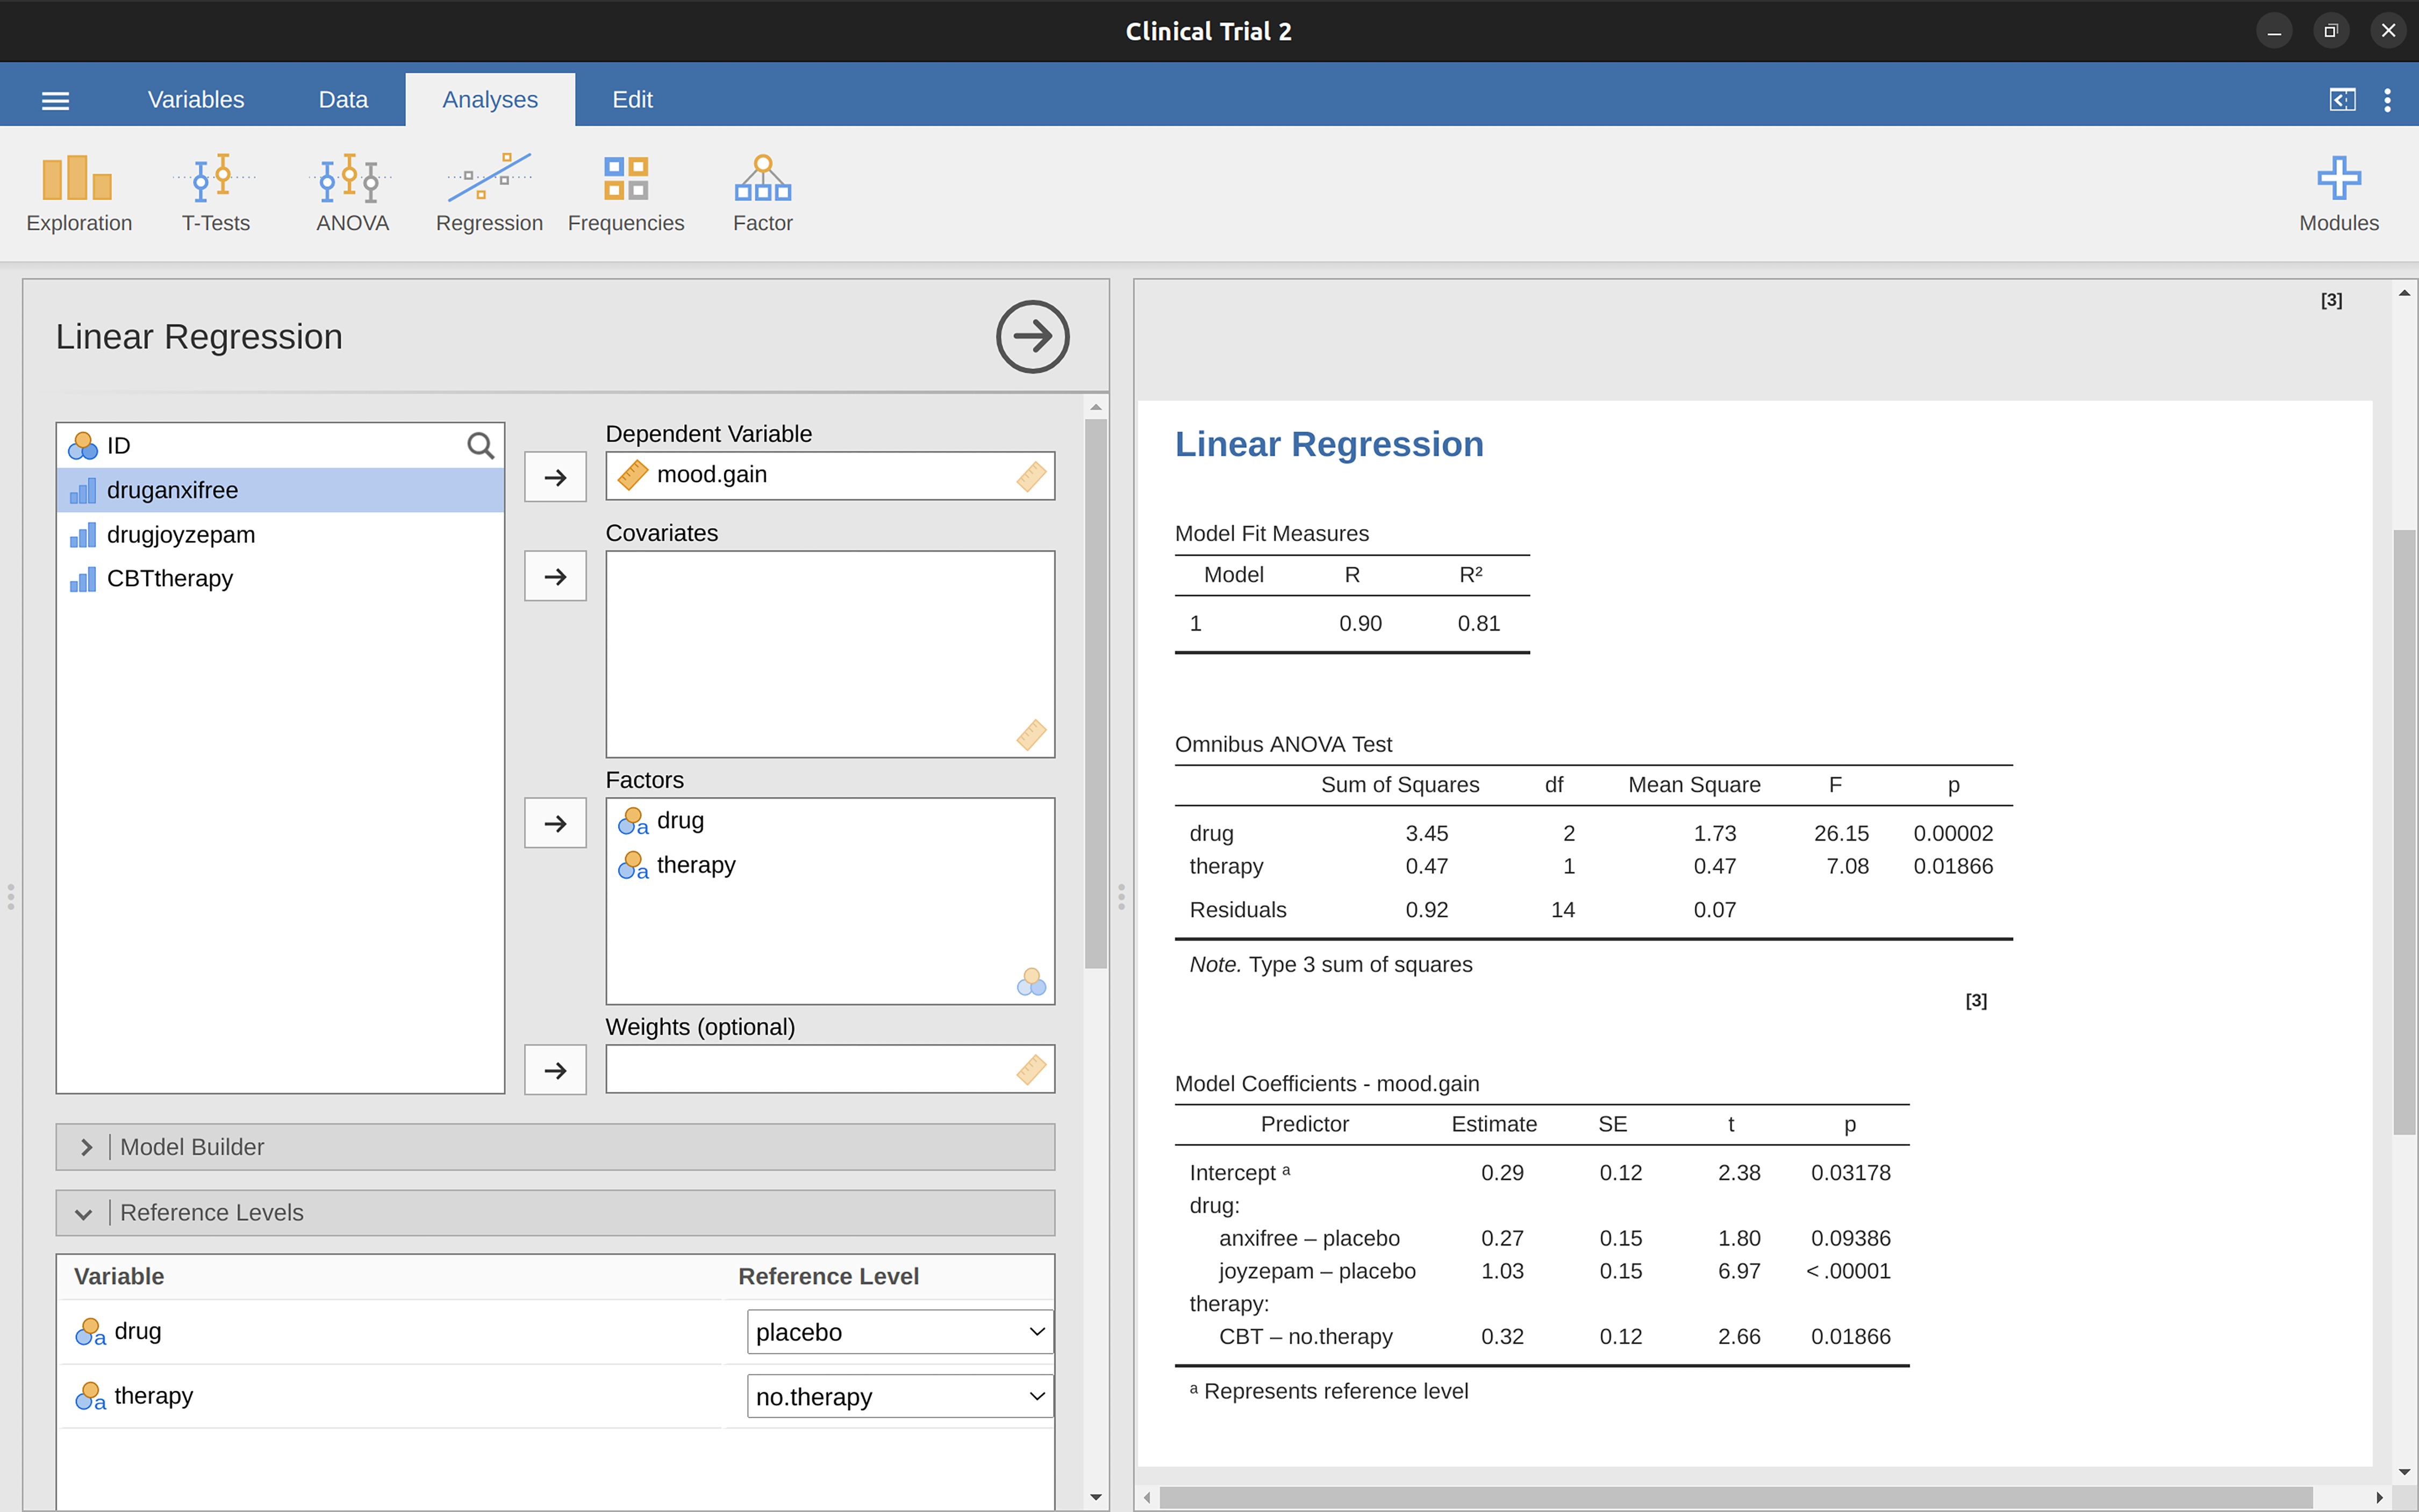
\includegraphics[width=1\textwidth,height=\textheight]{images/fig14-23.png} \hfill{}

\caption{\label{fig-fig14-23}Regression analysis with factors and
contrasts in jamovi, including omnibus ANOVA test results}

\end{figure}

If you also click on the `ANOVA' test checkbox under the `Model
Coefficients' - `Omnibus Test' option, we see that the \(F\)-statistic
is 26.15, the degrees of freedom are 2 and 14, and the \(p\)-value is
0.00002 (Figure~\ref{fig-fig14-23}). The numbers are identical to the
ones we obtained for the main effect of drug in our original ANOVA. Once
again, we see that ANOVA and regression are essentially the same. They
are both linear models, and the underlying statistical machinery for
ANOVA is identical to the machinery used in regression.

\hypertarget{degrees-of-freedom-as-parameter-counting}{%
\subsection{Degrees of freedom as parameter
counting!}\label{degrees-of-freedom-as-parameter-counting}}

At long last, I can finally give a definition of degrees of freedom that
I am happy with. Degrees of freedom are defined in terms of the number
of parameters that have to be estimated in a model. For a regression
model or an ANOVA, the number of parameters corresponds to the number of
regression coefficients (i.e.~\(b\)-values), including the intercept.
Keeping in mind that any \(F\)-test is always a comparison between two
models and the first df is the difference in the number of parameters.
For example, in the model comparison above, the null model (mood.gain
\textasciitilde{} therapyCBT) has two parameters: there's one regression
coefficient for the therapyCBT variable, and a second one for the
intercept. The alternative model (mood.gain \textasciitilde{}
druganxifree + drugjoyzepam + therapyCBT) has four parameters: one
regression coefficient for each of the three contrasts, and one more for
the intercept. So the degrees of freedom associated with the difference
between these two models is \(df_1 = 4 - 2 = 2\).

What about the case when there doesn't seem to be a null model? For
instance, you might be thinking of the \(F\)-test that shows up when you
select `F Test' under the `Linear Regression' - `Model Fit' options. I
originally described that as a test of the regression model as a whole.
However, that is still a comparison between two models. The null model
is the trivial model that only includes 1 regression coefficient, for
the intercept term. The alternative model contains \(K + 1\) regression
coefficients, one for each of the \(K\) predictor variables and one more
for the intercept. So the \(df\) value that you see in this \(F\)-test
is equal to \(df_1 = K + 1 - 1 = K\).

What about the second \(df\) value that appears in the \(F\)-test? This
always refers to the degrees of freedom associated with the residuals.
It is possible to think of this in terms of parameters too, but in a
slightly counter-intuitive way. Think of it like this. Suppose that the
total number of observations across the study as a whole is \(N\). If
you wanted to perfectly describe each of these \(N\) values, you need to
do so using, well\ldots{} \(N\) numbers. When you build a regression
model, what you're really doing is specifying that some of the numbers
need to perfectly describe the data. If your model has \(K\) predictors
and an intercept, then you've specified \(K + 1\) numbers. So, without
bothering to figure out exactly how this would be done, how many more
numbers do you think are going to be needed to transform a \(K + 1\)
parameter regression model into a perfect re-description of the raw
data? If you found yourself thinking that \((K + 1) + (N - K - 1) = N\),
and so the answer would have to be \(N - K - 1\), well done! That's
exactly right. In principle you can imagine an absurdly complicated
regression model that includes a parameter for every single data point,
and it would of course provide a perfect description of the data. This
model would contain \(N\) parameters in total, but we're interested in
the difference between the number of parameters required to describe
this full model (i.e.~\(N\)) and the number of parameters used by the
simpler regression model that you're actually interested in (i.e.,
\(K + 1\)), and so the second degrees of freedom in the \(F\) test is
\(df_2 = N - K - 1\), where \(K\) is the number of predictors (in a
regression model) or the number of contrasts (in an ANOVA). In the
example I gave above, there are \((N = 18\) observations in the data set
and \(K + 1 = 4\) regression coefficients associated with the ANOVA
model, so the degrees of freedom for the residuals is
\(df_2 = 18 - 4 = 14\).

\hypertarget{different-ways-to-specify-contrasts}{%
\section{Different ways to specify
contrasts}\label{different-ways-to-specify-contrasts}}

In the previous section, I showed you a method for converting a factor
into a collection of contrasts. In the method I showed you we specify a
set of binary variables in which we defined a table like
Table~\ref{tbl-tab14-11}.

\hypertarget{tbl-tab14-11}{}
 
  \providecommand{\huxb}[2]{\arrayrulecolor[RGB]{#1}\global\arrayrulewidth=#2pt}
  \providecommand{\huxvb}[2]{\color[RGB]{#1}\vrule width #2pt}
  \providecommand{\huxtpad}[1]{\rule{0pt}{#1}}
  \providecommand{\huxbpad}[1]{\rule[-#1]{0pt}{#1}}

\begin{table}[ht]
\caption{\label{tbl-tab14-11}Binary contrasts to discriminate between all three possible drugs }\tabularnewline

\begin{centerbox}
\begin{threeparttable}
\setlength{\tabcolsep}{0pt}
\begin{tabularx}{0.9\textwidth}{p{0.3\textwidth} p{0.3\textwidth} p{0.3\textwidth}}


\hhline{>{\huxb{0, 0, 0}{0.4}}->{\huxb{0, 0, 0}{0.4}}->{\huxb{0, 0, 0}{0.4}}-}
\arrayrulecolor{black}

\multicolumn{1}{!{\huxvb{0, 0, 0}{0}}p{0.3\textwidth}!{\huxvb{0, 0, 0}{0}}}{\hspace{0pt}\parbox[b]{0.3\textwidth-0pt-12pt}{\huxtpad{2pt + 1em}\centering \textbf{drug}\huxbpad{2pt}}} &
\multicolumn{1}{p{0.3\textwidth}!{\huxvb{0, 0, 0}{0}}}{\hspace{12pt}\parbox[b]{0.3\textwidth-12pt-12pt}{\huxtpad{2pt + 1em}\centering \textbf{druganxifree}\huxbpad{2pt}}} &
\multicolumn{1}{p{0.3\textwidth}!{\huxvb{0, 0, 0}{0}}}{\hspace{12pt}\parbox[b]{0.3\textwidth-12pt-0pt}{\huxtpad{2pt + 1em}\centering \textbf{drugjoyzepam}\huxbpad{2pt}}} \tabularnewline[-0.5pt]


\hhline{>{\huxb{0, 0, 0}{0.4}}->{\huxb{0, 0, 0}{0.4}}->{\huxb{0, 0, 0}{0.4}}-}
\arrayrulecolor{black}

\multicolumn{1}{!{\huxvb{0, 0, 0}{0}}p{0.3\textwidth}!{\huxvb{0, 0, 0}{0}}}{\hspace{0pt}\parbox[b]{0.3\textwidth-0pt-12pt}{\huxtpad{2pt + 1em}\centering ``placebo"\huxbpad{2pt}}} &
\multicolumn{1}{p{0.3\textwidth}!{\huxvb{0, 0, 0}{0}}}{\hspace{12pt}\parbox[b]{0.3\textwidth-12pt-12pt}{\huxtpad{2pt + 1em}\centering 0\huxbpad{2pt}}} &
\multicolumn{1}{p{0.3\textwidth}!{\huxvb{0, 0, 0}{0}}}{\hspace{12pt}\parbox[b]{0.3\textwidth-12pt-0pt}{\huxtpad{2pt + 1em}\centering 0\huxbpad{2pt}}} \tabularnewline[-0.5pt]


\hhline{}
\arrayrulecolor{black}

\multicolumn{1}{!{\huxvb{0, 0, 0}{0}}p{0.3\textwidth}!{\huxvb{0, 0, 0}{0}}}{\hspace{0pt}\parbox[b]{0.3\textwidth-0pt-12pt}{\huxtpad{2pt + 1em}\centering ``anxifree"\huxbpad{2pt}}} &
\multicolumn{1}{p{0.3\textwidth}!{\huxvb{0, 0, 0}{0}}}{\hspace{12pt}\parbox[b]{0.3\textwidth-12pt-12pt}{\huxtpad{2pt + 1em}\centering 1\huxbpad{2pt}}} &
\multicolumn{1}{p{0.3\textwidth}!{\huxvb{0, 0, 0}{0}}}{\hspace{12pt}\parbox[b]{0.3\textwidth-12pt-0pt}{\huxtpad{2pt + 1em}\centering 0\huxbpad{2pt}}} \tabularnewline[-0.5pt]


\hhline{}
\arrayrulecolor{black}

\multicolumn{1}{!{\huxvb{0, 0, 0}{0}}p{0.3\textwidth}!{\huxvb{0, 0, 0}{0}}}{\hspace{0pt}\parbox[b]{0.3\textwidth-0pt-12pt}{\huxtpad{2pt + 1em}\centering ``joyzepam"\huxbpad{2pt}}} &
\multicolumn{1}{p{0.3\textwidth}!{\huxvb{0, 0, 0}{0}}}{\hspace{12pt}\parbox[b]{0.3\textwidth-12pt-12pt}{\huxtpad{2pt + 1em}\centering 0\huxbpad{2pt}}} &
\multicolumn{1}{p{0.3\textwidth}!{\huxvb{0, 0, 0}{0}}}{\hspace{12pt}\parbox[b]{0.3\textwidth-12pt-0pt}{\huxtpad{2pt + 1em}\centering 1\huxbpad{2pt}}} \tabularnewline[-0.5pt]


\hhline{>{\huxb{0, 0, 0}{0.4}}->{\huxb{0, 0, 0}{0.4}}->{\huxb{0, 0, 0}{0.4}}-}
\arrayrulecolor{black}
\end{tabularx} 

\end{threeparttable}\par\end{centerbox}

\end{table}
 

Each row in the table corresponds to one of the factor levels, and each
column corresponds to one of the contrasts. This table, which always has
one more row than columns, has a special name. It is called a contrast
matrix. However, there are lots of different ways to specify a contrast
matrix. In this section I discuss a few of the standard contrast
matrices that statisticians use and how you can use them in jamovi. If
you're planning to read the section on
\protect\hyperlink{factorial-anova-3-unbalanced-designs}{Factorial ANOVA
3: unbalanced designs} later on, it's worth reading this section
carefully. If not, you can get away with skimming it, because the choice
of contrasts doesn't matter much for balanced designs.

\hypertarget{treatment-contrasts}{%
\subsection{Treatment contrasts}\label{treatment-contrasts}}

In the particular kind of contrasts that I've described above, one level
of the factor is special, and acts as a kind of ``baseline'' category
(i.e., placebo in our example), against which the other two are defined.
The name for these kinds of contrasts is treatment contrasts, also known
as ``dummy coding''. In this contrast each level of the factor is
compared to a base reference level, and the base reference level is the
value of the intercept.

The name reflects the fact that these contrasts are natural and sensible
when one of the categories in your factor really is special and actually
does represent a baseline. That makes sense in our clinical trial
example. The placebo condition corresponds to the situation where you
don't give people any real drugs, and so it's special. The other two
conditions are defined in relation to the placebo. In one case you
replace the placebo with Anxifree, and in the other case your replace it
with Joyzepam.

The table shown above is a matrix of treatment contrasts for a factor
that has 3 levels. But suppose I want a matrix of treatment contrasts
for a factor with 5 levels? You would set this out like
Table~\ref{tbl-tab14-12}.

\hypertarget{tbl-tab14-12}{}
 
  \providecommand{\huxb}[2]{\arrayrulecolor[RGB]{#1}\global\arrayrulewidth=#2pt}
  \providecommand{\huxvb}[2]{\color[RGB]{#1}\vrule width #2pt}
  \providecommand{\huxtpad}[1]{\rule{0pt}{#1}}
  \providecommand{\huxbpad}[1]{\rule[-#1]{0pt}{#1}}

\begin{table}[ht]
\caption{\label{tbl-tab14-12}Matrix of treatment contrasts with 5 levels }\tabularnewline

\begin{centerbox}
\begin{threeparttable}
\setlength{\tabcolsep}{0pt}
\begin{tabularx}{0.9\textwidth}{p{0.18\textwidth} p{0.18\textwidth} p{0.18\textwidth} p{0.18\textwidth} p{0.18\textwidth}}


\hhline{>{\huxb{0, 0, 0}{0.4}}->{\huxb{0, 0, 0}{0.4}}->{\huxb{0, 0, 0}{0.4}}->{\huxb{0, 0, 0}{0.4}}->{\huxb{0, 0, 0}{0.4}}-}
\arrayrulecolor{black}

\multicolumn{1}{!{\huxvb{0, 0, 0}{0}}p{0.18\textwidth}!{\huxvb{0, 0, 0}{0}}}{\hspace{0pt}\parbox[b]{0.18\textwidth-0pt-12pt}{\huxtpad{2pt + 1em}\centering \textbf{Level}\huxbpad{2pt}}} &
\multicolumn{1}{p{0.18\textwidth}!{\huxvb{0, 0, 0}{0}}}{\hspace{12pt}\parbox[b]{0.18\textwidth-12pt-12pt}{\huxtpad{2pt + 1em}\centering \textbf{2}\huxbpad{2pt}}} &
\multicolumn{1}{p{0.18\textwidth}!{\huxvb{0, 0, 0}{0}}}{\hspace{12pt}\parbox[b]{0.18\textwidth-12pt-12pt}{\huxtpad{2pt + 1em}\centering \textbf{3}\huxbpad{2pt}}} &
\multicolumn{1}{p{0.18\textwidth}!{\huxvb{0, 0, 0}{0}}}{\hspace{12pt}\parbox[b]{0.18\textwidth-12pt-12pt}{\huxtpad{2pt + 1em}\centering \textbf{4}\huxbpad{2pt}}} &
\multicolumn{1}{p{0.18\textwidth}!{\huxvb{0, 0, 0}{0}}}{\hspace{12pt}\parbox[b]{0.18\textwidth-12pt-0pt}{\huxtpad{2pt + 1em}\centering \textbf{5}\huxbpad{2pt}}} \tabularnewline[-0.5pt]


\hhline{>{\huxb{0, 0, 0}{0.4}}->{\huxb{0, 0, 0}{0.4}}->{\huxb{0, 0, 0}{0.4}}->{\huxb{0, 0, 0}{0.4}}->{\huxb{0, 0, 0}{0.4}}-}
\arrayrulecolor{black}

\multicolumn{1}{!{\huxvb{0, 0, 0}{0}}p{0.18\textwidth}!{\huxvb{0, 0, 0}{0}}}{\hspace{0pt}\parbox[b]{0.18\textwidth-0pt-12pt}{\huxtpad{2pt + 1em}\centering 1\huxbpad{2pt}}} &
\multicolumn{1}{p{0.18\textwidth}!{\huxvb{0, 0, 0}{0}}}{\hspace{12pt}\parbox[b]{0.18\textwidth-12pt-12pt}{\huxtpad{2pt + 1em}\centering 0\huxbpad{2pt}}} &
\multicolumn{1}{p{0.18\textwidth}!{\huxvb{0, 0, 0}{0}}}{\hspace{12pt}\parbox[b]{0.18\textwidth-12pt-12pt}{\huxtpad{2pt + 1em}\centering 0\huxbpad{2pt}}} &
\multicolumn{1}{p{0.18\textwidth}!{\huxvb{0, 0, 0}{0}}}{\hspace{12pt}\parbox[b]{0.18\textwidth-12pt-12pt}{\huxtpad{2pt + 1em}\centering 0\huxbpad{2pt}}} &
\multicolumn{1}{p{0.18\textwidth}!{\huxvb{0, 0, 0}{0}}}{\hspace{12pt}\parbox[b]{0.18\textwidth-12pt-0pt}{\huxtpad{2pt + 1em}\centering 0\huxbpad{2pt}}} \tabularnewline[-0.5pt]


\hhline{}
\arrayrulecolor{black}

\multicolumn{1}{!{\huxvb{0, 0, 0}{0}}p{0.18\textwidth}!{\huxvb{0, 0, 0}{0}}}{\hspace{0pt}\parbox[b]{0.18\textwidth-0pt-12pt}{\huxtpad{2pt + 1em}\centering 2\huxbpad{2pt}}} &
\multicolumn{1}{p{0.18\textwidth}!{\huxvb{0, 0, 0}{0}}}{\hspace{12pt}\parbox[b]{0.18\textwidth-12pt-12pt}{\huxtpad{2pt + 1em}\centering 1\huxbpad{2pt}}} &
\multicolumn{1}{p{0.18\textwidth}!{\huxvb{0, 0, 0}{0}}}{\hspace{12pt}\parbox[b]{0.18\textwidth-12pt-12pt}{\huxtpad{2pt + 1em}\centering 0\huxbpad{2pt}}} &
\multicolumn{1}{p{0.18\textwidth}!{\huxvb{0, 0, 0}{0}}}{\hspace{12pt}\parbox[b]{0.18\textwidth-12pt-12pt}{\huxtpad{2pt + 1em}\centering 0\huxbpad{2pt}}} &
\multicolumn{1}{p{0.18\textwidth}!{\huxvb{0, 0, 0}{0}}}{\hspace{12pt}\parbox[b]{0.18\textwidth-12pt-0pt}{\huxtpad{2pt + 1em}\centering 0\huxbpad{2pt}}} \tabularnewline[-0.5pt]


\hhline{}
\arrayrulecolor{black}

\multicolumn{1}{!{\huxvb{0, 0, 0}{0}}p{0.18\textwidth}!{\huxvb{0, 0, 0}{0}}}{\hspace{0pt}\parbox[b]{0.18\textwidth-0pt-12pt}{\huxtpad{2pt + 1em}\centering 3\huxbpad{2pt}}} &
\multicolumn{1}{p{0.18\textwidth}!{\huxvb{0, 0, 0}{0}}}{\hspace{12pt}\parbox[b]{0.18\textwidth-12pt-12pt}{\huxtpad{2pt + 1em}\centering 0\huxbpad{2pt}}} &
\multicolumn{1}{p{0.18\textwidth}!{\huxvb{0, 0, 0}{0}}}{\hspace{12pt}\parbox[b]{0.18\textwidth-12pt-12pt}{\huxtpad{2pt + 1em}\centering 1\huxbpad{2pt}}} &
\multicolumn{1}{p{0.18\textwidth}!{\huxvb{0, 0, 0}{0}}}{\hspace{12pt}\parbox[b]{0.18\textwidth-12pt-12pt}{\huxtpad{2pt + 1em}\centering 0\huxbpad{2pt}}} &
\multicolumn{1}{p{0.18\textwidth}!{\huxvb{0, 0, 0}{0}}}{\hspace{12pt}\parbox[b]{0.18\textwidth-12pt-0pt}{\huxtpad{2pt + 1em}\centering 0\huxbpad{2pt}}} \tabularnewline[-0.5pt]


\hhline{}
\arrayrulecolor{black}

\multicolumn{1}{!{\huxvb{0, 0, 0}{0}}p{0.18\textwidth}!{\huxvb{0, 0, 0}{0}}}{\hspace{0pt}\parbox[b]{0.18\textwidth-0pt-12pt}{\huxtpad{2pt + 1em}\centering 4\huxbpad{2pt}}} &
\multicolumn{1}{p{0.18\textwidth}!{\huxvb{0, 0, 0}{0}}}{\hspace{12pt}\parbox[b]{0.18\textwidth-12pt-12pt}{\huxtpad{2pt + 1em}\centering 0\huxbpad{2pt}}} &
\multicolumn{1}{p{0.18\textwidth}!{\huxvb{0, 0, 0}{0}}}{\hspace{12pt}\parbox[b]{0.18\textwidth-12pt-12pt}{\huxtpad{2pt + 1em}\centering 0\huxbpad{2pt}}} &
\multicolumn{1}{p{0.18\textwidth}!{\huxvb{0, 0, 0}{0}}}{\hspace{12pt}\parbox[b]{0.18\textwidth-12pt-12pt}{\huxtpad{2pt + 1em}\centering 1\huxbpad{2pt}}} &
\multicolumn{1}{p{0.18\textwidth}!{\huxvb{0, 0, 0}{0}}}{\hspace{12pt}\parbox[b]{0.18\textwidth-12pt-0pt}{\huxtpad{2pt + 1em}\centering 0\huxbpad{2pt}}} \tabularnewline[-0.5pt]


\hhline{}
\arrayrulecolor{black}

\multicolumn{1}{!{\huxvb{0, 0, 0}{0}}p{0.18\textwidth}!{\huxvb{0, 0, 0}{0}}}{\hspace{0pt}\parbox[b]{0.18\textwidth-0pt-12pt}{\huxtpad{2pt + 1em}\centering 5\huxbpad{2pt}}} &
\multicolumn{1}{p{0.18\textwidth}!{\huxvb{0, 0, 0}{0}}}{\hspace{12pt}\parbox[b]{0.18\textwidth-12pt-12pt}{\huxtpad{2pt + 1em}\centering 0\huxbpad{2pt}}} &
\multicolumn{1}{p{0.18\textwidth}!{\huxvb{0, 0, 0}{0}}}{\hspace{12pt}\parbox[b]{0.18\textwidth-12pt-12pt}{\huxtpad{2pt + 1em}\centering 0\huxbpad{2pt}}} &
\multicolumn{1}{p{0.18\textwidth}!{\huxvb{0, 0, 0}{0}}}{\hspace{12pt}\parbox[b]{0.18\textwidth-12pt-12pt}{\huxtpad{2pt + 1em}\centering 0\huxbpad{2pt}}} &
\multicolumn{1}{p{0.18\textwidth}!{\huxvb{0, 0, 0}{0}}}{\hspace{12pt}\parbox[b]{0.18\textwidth-12pt-0pt}{\huxtpad{2pt + 1em}\centering 1\huxbpad{2pt}}} \tabularnewline[-0.5pt]


\hhline{>{\huxb{0, 0, 0}{0.4}}->{\huxb{0, 0, 0}{0.4}}->{\huxb{0, 0, 0}{0.4}}->{\huxb{0, 0, 0}{0.4}}->{\huxb{0, 0, 0}{0.4}}-}
\arrayrulecolor{black}
\end{tabularx} 

\end{threeparttable}\par\end{centerbox}

\end{table}
 

In this example, the first contrast is level 2 compared with level 1,
the second contrast is level 3 compared with level 1, and so on. Notice
that, by default, the \emph{first} level of the factor is always treated
as the baseline category (i.e., it's the one that has all zeros and
doesn't have an explicit contrast associated with it). In jamovi you can
change which category is the first level of the factor by manipulating
the order of the levels of the variable shown in the `Data Variable'
window (double click on the name of the variable in the spreadsheet
column to bring up the `Data Variable' view.

\hypertarget{helmert-contrasts}{%
\subsection{Helmert contrasts}\label{helmert-contrasts}}

Treatment contrasts are useful for a lot of situations. However, they
make most sense in the situation when there really is a baseline
category, and you want to assess all the other groups in relation to
that one. In other situations, however, no such baseline category
exists, and it may make more sense to compare each group to the mean of
the other groups. This is where we meet Helmert contrasts, generated by
the `helmert' option in the jamovi `ANOVA' - `Contrasts' selection box.
The idea behind Helmert contrasts is to compare each group to the mean
of the ``previous'' ones. That is, the first contrast represents the
difference between group 2 and group 1, the second contrast represents
the difference between group 3 and the mean of groups 1 and 2, and so
on. This translates to a contrast matrix that looks like
Table~\ref{tbl-tab14-13} for a factor with five levels.

\hypertarget{tbl-tab14-13}{}
 
  \providecommand{\huxb}[2]{\arrayrulecolor[RGB]{#1}\global\arrayrulewidth=#2pt}
  \providecommand{\huxvb}[2]{\color[RGB]{#1}\vrule width #2pt}
  \providecommand{\huxtpad}[1]{\rule{0pt}{#1}}
  \providecommand{\huxbpad}[1]{\rule[-#1]{0pt}{#1}}

\begin{table}[ht]
\caption{\label{tbl-tab14-13}Matrix of helmert contrasts with 5 levels }\tabularnewline

\begin{centerbox}
\begin{threeparttable}
\setlength{\tabcolsep}{0pt}
\begin{tabularx}{0.9\textwidth}{p{0.18\textwidth} p{0.18\textwidth} p{0.18\textwidth} p{0.18\textwidth} p{0.18\textwidth}}


\hhline{>{\huxb{0, 0, 0}{0.4}}->{\huxb{0, 0, 0}{0.4}}->{\huxb{0, 0, 0}{0.4}}->{\huxb{0, 0, 0}{0.4}}->{\huxb{0, 0, 0}{0.4}}-}
\arrayrulecolor{black}

\multicolumn{1}{!{\huxvb{0, 0, 0}{0}}p{0.18\textwidth}!{\huxvb{0, 0, 0}{0}}}{\hspace{0pt}\parbox[b]{0.18\textwidth-0pt-12pt}{\huxtpad{2pt + 1em}\centering \textbf{1}\huxbpad{2pt}}} &
\multicolumn{1}{p{0.18\textwidth}!{\huxvb{0, 0, 0}{0}}}{\hspace{12pt}\parbox[b]{0.18\textwidth-12pt-12pt}{\huxtpad{2pt + 1em}\centering \textbf{-1}\huxbpad{2pt}}} &
\multicolumn{1}{p{0.18\textwidth}!{\huxvb{0, 0, 0}{0}}}{\hspace{12pt}\parbox[b]{0.18\textwidth-12pt-12pt}{\huxtpad{2pt + 1em}\centering \textbf{-1}\huxbpad{2pt}}} &
\multicolumn{1}{p{0.18\textwidth}!{\huxvb{0, 0, 0}{0}}}{\hspace{12pt}\parbox[b]{0.18\textwidth-12pt-12pt}{\huxtpad{2pt + 1em}\centering \textbf{-1}\huxbpad{2pt}}} &
\multicolumn{1}{p{0.18\textwidth}!{\huxvb{0, 0, 0}{0}}}{\hspace{12pt}\parbox[b]{0.18\textwidth-12pt-0pt}{\huxtpad{2pt + 1em}\centering \textbf{-1}\huxbpad{2pt}}} \tabularnewline[-0.5pt]


\hhline{>{\huxb{0, 0, 0}{0.4}}->{\huxb{0, 0, 0}{0.4}}->{\huxb{0, 0, 0}{0.4}}->{\huxb{0, 0, 0}{0.4}}->{\huxb{0, 0, 0}{0.4}}-}
\arrayrulecolor{black}

\multicolumn{1}{!{\huxvb{0, 0, 0}{0}}p{0.18\textwidth}!{\huxvb{0, 0, 0}{0}}}{\hspace{0pt}\parbox[b]{0.18\textwidth-0pt-12pt}{\huxtpad{2pt + 1em}\centering 2\huxbpad{2pt}}} &
\multicolumn{1}{p{0.18\textwidth}!{\huxvb{0, 0, 0}{0}}}{\hspace{12pt}\parbox[b]{0.18\textwidth-12pt-12pt}{\huxtpad{2pt + 1em}\centering 1\huxbpad{2pt}}} &
\multicolumn{1}{p{0.18\textwidth}!{\huxvb{0, 0, 0}{0}}}{\hspace{12pt}\parbox[b]{0.18\textwidth-12pt-12pt}{\huxtpad{2pt + 1em}\centering -1\huxbpad{2pt}}} &
\multicolumn{1}{p{0.18\textwidth}!{\huxvb{0, 0, 0}{0}}}{\hspace{12pt}\parbox[b]{0.18\textwidth-12pt-12pt}{\huxtpad{2pt + 1em}\centering -1\huxbpad{2pt}}} &
\multicolumn{1}{p{0.18\textwidth}!{\huxvb{0, 0, 0}{0}}}{\hspace{12pt}\parbox[b]{0.18\textwidth-12pt-0pt}{\huxtpad{2pt + 1em}\centering -1\huxbpad{2pt}}} \tabularnewline[-0.5pt]


\hhline{}
\arrayrulecolor{black}

\multicolumn{1}{!{\huxvb{0, 0, 0}{0}}p{0.18\textwidth}!{\huxvb{0, 0, 0}{0}}}{\hspace{0pt}\parbox[b]{0.18\textwidth-0pt-12pt}{\huxtpad{2pt + 1em}\centering 3\huxbpad{2pt}}} &
\multicolumn{1}{p{0.18\textwidth}!{\huxvb{0, 0, 0}{0}}}{\hspace{12pt}\parbox[b]{0.18\textwidth-12pt-12pt}{\huxtpad{2pt + 1em}\centering 0\huxbpad{2pt}}} &
\multicolumn{1}{p{0.18\textwidth}!{\huxvb{0, 0, 0}{0}}}{\hspace{12pt}\parbox[b]{0.18\textwidth-12pt-12pt}{\huxtpad{2pt + 1em}\centering 2\huxbpad{2pt}}} &
\multicolumn{1}{p{0.18\textwidth}!{\huxvb{0, 0, 0}{0}}}{\hspace{12pt}\parbox[b]{0.18\textwidth-12pt-12pt}{\huxtpad{2pt + 1em}\centering -1\huxbpad{2pt}}} &
\multicolumn{1}{p{0.18\textwidth}!{\huxvb{0, 0, 0}{0}}}{\hspace{12pt}\parbox[b]{0.18\textwidth-12pt-0pt}{\huxtpad{2pt + 1em}\centering -1\huxbpad{2pt}}} \tabularnewline[-0.5pt]


\hhline{}
\arrayrulecolor{black}

\multicolumn{1}{!{\huxvb{0, 0, 0}{0}}p{0.18\textwidth}!{\huxvb{0, 0, 0}{0}}}{\hspace{0pt}\parbox[b]{0.18\textwidth-0pt-12pt}{\huxtpad{2pt + 1em}\centering 4\huxbpad{2pt}}} &
\multicolumn{1}{p{0.18\textwidth}!{\huxvb{0, 0, 0}{0}}}{\hspace{12pt}\parbox[b]{0.18\textwidth-12pt-12pt}{\huxtpad{2pt + 1em}\centering 0\huxbpad{2pt}}} &
\multicolumn{1}{p{0.18\textwidth}!{\huxvb{0, 0, 0}{0}}}{\hspace{12pt}\parbox[b]{0.18\textwidth-12pt-12pt}{\huxtpad{2pt + 1em}\centering 0\huxbpad{2pt}}} &
\multicolumn{1}{p{0.18\textwidth}!{\huxvb{0, 0, 0}{0}}}{\hspace{12pt}\parbox[b]{0.18\textwidth-12pt-12pt}{\huxtpad{2pt + 1em}\centering 3\huxbpad{2pt}}} &
\multicolumn{1}{p{0.18\textwidth}!{\huxvb{0, 0, 0}{0}}}{\hspace{12pt}\parbox[b]{0.18\textwidth-12pt-0pt}{\huxtpad{2pt + 1em}\centering -1\huxbpad{2pt}}} \tabularnewline[-0.5pt]


\hhline{}
\arrayrulecolor{black}

\multicolumn{1}{!{\huxvb{0, 0, 0}{0}}p{0.18\textwidth}!{\huxvb{0, 0, 0}{0}}}{\hspace{0pt}\parbox[b]{0.18\textwidth-0pt-12pt}{\huxtpad{2pt + 1em}\centering 5\huxbpad{2pt}}} &
\multicolumn{1}{p{0.18\textwidth}!{\huxvb{0, 0, 0}{0}}}{\hspace{12pt}\parbox[b]{0.18\textwidth-12pt-12pt}{\huxtpad{2pt + 1em}\centering 0\huxbpad{2pt}}} &
\multicolumn{1}{p{0.18\textwidth}!{\huxvb{0, 0, 0}{0}}}{\hspace{12pt}\parbox[b]{0.18\textwidth-12pt-12pt}{\huxtpad{2pt + 1em}\centering 0\huxbpad{2pt}}} &
\multicolumn{1}{p{0.18\textwidth}!{\huxvb{0, 0, 0}{0}}}{\hspace{12pt}\parbox[b]{0.18\textwidth-12pt-12pt}{\huxtpad{2pt + 1em}\centering 0\huxbpad{2pt}}} &
\multicolumn{1}{p{0.18\textwidth}!{\huxvb{0, 0, 0}{0}}}{\hspace{12pt}\parbox[b]{0.18\textwidth-12pt-0pt}{\huxtpad{2pt + 1em}\centering 4\huxbpad{2pt}}} \tabularnewline[-0.5pt]


\hhline{>{\huxb{0, 0, 0}{0.4}}->{\huxb{0, 0, 0}{0.4}}->{\huxb{0, 0, 0}{0.4}}->{\huxb{0, 0, 0}{0.4}}->{\huxb{0, 0, 0}{0.4}}-}
\arrayrulecolor{black}
\end{tabularx} 

\end{threeparttable}\par\end{centerbox}

\end{table}
 

One useful thing about Helmert contrasts is that every contrast sums to
zero (i.e., all the columns sum to zero). This has the consequence that,
when we interpret the ANOVA as a regression, the intercept term
corresponds to the grand mean \(\mu_{..}\) if we are using Helmert
contrasts. Compare this to treatment contrasts, in which the intercept
term corresponds to the group mean for the baseline category. This
property can be very useful in some situations. It doesn't matter very
much if you have a balanced design, which we've been assuming so far,
but it will turn out to be important later when we consider
\href{Factorial\%20ANOVA:\%20unbalanced\%20designs}{unbalanced designs}.
In fact, the main reason why I've even bothered to include this section
is that contrasts become important if you want to understand unbalanced
ANOVA.

\hypertarget{sum-to-zero-contrasts}{%
\subsection{Sum to zero contrasts}\label{sum-to-zero-contrasts}}

The third option that I should briefly mention are ``sum to zero''
contrasts, called ``Simple'' contrasts in jamovi, which are used to
construct pairwise comparisons between groups. Specifically, each
contrast encodes the difference between one of the groups and a baseline
category, which in this case corresponds to the first group
(Table~\ref{tbl-tab14-14}).

\hypertarget{tbl-tab14-14}{}
 
  \providecommand{\huxb}[2]{\arrayrulecolor[RGB]{#1}\global\arrayrulewidth=#2pt}
  \providecommand{\huxvb}[2]{\color[RGB]{#1}\vrule width #2pt}
  \providecommand{\huxtpad}[1]{\rule{0pt}{#1}}
  \providecommand{\huxbpad}[1]{\rule[-#1]{0pt}{#1}}

\begin{table}[ht]
\caption{\label{tbl-tab14-14}Matrix of ``sum to'' zero contrasts with 5 levels }\tabularnewline

\begin{centerbox}
\begin{threeparttable}
\setlength{\tabcolsep}{0pt}
\begin{tabularx}{0.9\textwidth}{p{0.18\textwidth} p{0.18\textwidth} p{0.18\textwidth} p{0.18\textwidth} p{0.18\textwidth}}


\hhline{>{\huxb{0, 0, 0}{0.4}}->{\huxb{0, 0, 0}{0.4}}->{\huxb{0, 0, 0}{0.4}}->{\huxb{0, 0, 0}{0.4}}->{\huxb{0, 0, 0}{0.4}}-}
\arrayrulecolor{black}

\multicolumn{1}{!{\huxvb{0, 0, 0}{0}}p{0.18\textwidth}!{\huxvb{0, 0, 0}{0}}}{\hspace{0pt}\parbox[b]{0.18\textwidth-0pt-12pt}{\huxtpad{2pt + 1em}\centering \textbf{1}\huxbpad{2pt}}} &
\multicolumn{1}{p{0.18\textwidth}!{\huxvb{0, 0, 0}{0}}}{\hspace{12pt}\parbox[b]{0.18\textwidth-12pt-12pt}{\huxtpad{2pt + 1em}\centering \textbf{-1}\huxbpad{2pt}}} &
\multicolumn{1}{p{0.18\textwidth}!{\huxvb{0, 0, 0}{0}}}{\hspace{12pt}\parbox[b]{0.18\textwidth-12pt-12pt}{\huxtpad{2pt + 1em}\centering \textbf{-1}\huxbpad{2pt}}} &
\multicolumn{1}{p{0.18\textwidth}!{\huxvb{0, 0, 0}{0}}}{\hspace{12pt}\parbox[b]{0.18\textwidth-12pt-12pt}{\huxtpad{2pt + 1em}\centering \textbf{-1}\huxbpad{2pt}}} &
\multicolumn{1}{p{0.18\textwidth}!{\huxvb{0, 0, 0}{0}}}{\hspace{12pt}\parbox[b]{0.18\textwidth-12pt-0pt}{\huxtpad{2pt + 1em}\centering \textbf{-1}\huxbpad{2pt}}} \tabularnewline[-0.5pt]


\hhline{>{\huxb{0, 0, 0}{0.4}}->{\huxb{0, 0, 0}{0.4}}->{\huxb{0, 0, 0}{0.4}}->{\huxb{0, 0, 0}{0.4}}->{\huxb{0, 0, 0}{0.4}}-}
\arrayrulecolor{black}

\multicolumn{1}{!{\huxvb{0, 0, 0}{0}}p{0.18\textwidth}!{\huxvb{0, 0, 0}{0}}}{\hspace{0pt}\parbox[b]{0.18\textwidth-0pt-12pt}{\huxtpad{2pt + 1em}\centering 2\huxbpad{2pt}}} &
\multicolumn{1}{p{0.18\textwidth}!{\huxvb{0, 0, 0}{0}}}{\hspace{12pt}\parbox[b]{0.18\textwidth-12pt-12pt}{\huxtpad{2pt + 1em}\centering 1\huxbpad{2pt}}} &
\multicolumn{1}{p{0.18\textwidth}!{\huxvb{0, 0, 0}{0}}}{\hspace{12pt}\parbox[b]{0.18\textwidth-12pt-12pt}{\huxtpad{2pt + 1em}\centering 0\huxbpad{2pt}}} &
\multicolumn{1}{p{0.18\textwidth}!{\huxvb{0, 0, 0}{0}}}{\hspace{12pt}\parbox[b]{0.18\textwidth-12pt-12pt}{\huxtpad{2pt + 1em}\centering 0\huxbpad{2pt}}} &
\multicolumn{1}{p{0.18\textwidth}!{\huxvb{0, 0, 0}{0}}}{\hspace{12pt}\parbox[b]{0.18\textwidth-12pt-0pt}{\huxtpad{2pt + 1em}\centering 0\huxbpad{2pt}}} \tabularnewline[-0.5pt]


\hhline{}
\arrayrulecolor{black}

\multicolumn{1}{!{\huxvb{0, 0, 0}{0}}p{0.18\textwidth}!{\huxvb{0, 0, 0}{0}}}{\hspace{0pt}\parbox[b]{0.18\textwidth-0pt-12pt}{\huxtpad{2pt + 1em}\centering 3\huxbpad{2pt}}} &
\multicolumn{1}{p{0.18\textwidth}!{\huxvb{0, 0, 0}{0}}}{\hspace{12pt}\parbox[b]{0.18\textwidth-12pt-12pt}{\huxtpad{2pt + 1em}\centering 0\huxbpad{2pt}}} &
\multicolumn{1}{p{0.18\textwidth}!{\huxvb{0, 0, 0}{0}}}{\hspace{12pt}\parbox[b]{0.18\textwidth-12pt-12pt}{\huxtpad{2pt + 1em}\centering 1\huxbpad{2pt}}} &
\multicolumn{1}{p{0.18\textwidth}!{\huxvb{0, 0, 0}{0}}}{\hspace{12pt}\parbox[b]{0.18\textwidth-12pt-12pt}{\huxtpad{2pt + 1em}\centering 0\huxbpad{2pt}}} &
\multicolumn{1}{p{0.18\textwidth}!{\huxvb{0, 0, 0}{0}}}{\hspace{12pt}\parbox[b]{0.18\textwidth-12pt-0pt}{\huxtpad{2pt + 1em}\centering 0\huxbpad{2pt}}} \tabularnewline[-0.5pt]


\hhline{}
\arrayrulecolor{black}

\multicolumn{1}{!{\huxvb{0, 0, 0}{0}}p{0.18\textwidth}!{\huxvb{0, 0, 0}{0}}}{\hspace{0pt}\parbox[b]{0.18\textwidth-0pt-12pt}{\huxtpad{2pt + 1em}\centering 4\huxbpad{2pt}}} &
\multicolumn{1}{p{0.18\textwidth}!{\huxvb{0, 0, 0}{0}}}{\hspace{12pt}\parbox[b]{0.18\textwidth-12pt-12pt}{\huxtpad{2pt + 1em}\centering 0\huxbpad{2pt}}} &
\multicolumn{1}{p{0.18\textwidth}!{\huxvb{0, 0, 0}{0}}}{\hspace{12pt}\parbox[b]{0.18\textwidth-12pt-12pt}{\huxtpad{2pt + 1em}\centering 0\huxbpad{2pt}}} &
\multicolumn{1}{p{0.18\textwidth}!{\huxvb{0, 0, 0}{0}}}{\hspace{12pt}\parbox[b]{0.18\textwidth-12pt-12pt}{\huxtpad{2pt + 1em}\centering 1\huxbpad{2pt}}} &
\multicolumn{1}{p{0.18\textwidth}!{\huxvb{0, 0, 0}{0}}}{\hspace{12pt}\parbox[b]{0.18\textwidth-12pt-0pt}{\huxtpad{2pt + 1em}\centering 0\huxbpad{2pt}}} \tabularnewline[-0.5pt]


\hhline{}
\arrayrulecolor{black}

\multicolumn{1}{!{\huxvb{0, 0, 0}{0}}p{0.18\textwidth}!{\huxvb{0, 0, 0}{0}}}{\hspace{0pt}\parbox[b]{0.18\textwidth-0pt-12pt}{\huxtpad{2pt + 1em}\centering 5\huxbpad{2pt}}} &
\multicolumn{1}{p{0.18\textwidth}!{\huxvb{0, 0, 0}{0}}}{\hspace{12pt}\parbox[b]{0.18\textwidth-12pt-12pt}{\huxtpad{2pt + 1em}\centering 0\huxbpad{2pt}}} &
\multicolumn{1}{p{0.18\textwidth}!{\huxvb{0, 0, 0}{0}}}{\hspace{12pt}\parbox[b]{0.18\textwidth-12pt-12pt}{\huxtpad{2pt + 1em}\centering 0\huxbpad{2pt}}} &
\multicolumn{1}{p{0.18\textwidth}!{\huxvb{0, 0, 0}{0}}}{\hspace{12pt}\parbox[b]{0.18\textwidth-12pt-12pt}{\huxtpad{2pt + 1em}\centering 0\huxbpad{2pt}}} &
\multicolumn{1}{p{0.18\textwidth}!{\huxvb{0, 0, 0}{0}}}{\hspace{12pt}\parbox[b]{0.18\textwidth-12pt-0pt}{\huxtpad{2pt + 1em}\centering 1\huxbpad{2pt}}} \tabularnewline[-0.5pt]


\hhline{>{\huxb{0, 0, 0}{0.4}}->{\huxb{0, 0, 0}{0.4}}->{\huxb{0, 0, 0}{0.4}}->{\huxb{0, 0, 0}{0.4}}->{\huxb{0, 0, 0}{0.4}}-}
\arrayrulecolor{black}
\end{tabularx} 

\end{threeparttable}\par\end{centerbox}

\end{table}
 

Much like Helmert contrasts, we see that each column sums to zero, which
means that the intercept term corresponds to the grand mean when ANOVA
is treated as a regression model. When interpreting these contrasts, the
thing to recognise is that each of these contrasts is a pairwise
comparison between group 1 and one of the other four groups.
Specifically, contrast 1 corresponds to a ``group 2 minus group 1''
comparison, contrast 2 corresponds to a ``group 3 minus group 1''
comparison, and so on.\footnote{What's the difference between treatment
  and simple contrasts, I hear you ask? Well, as a basic example
  consider a gender main effect, with \(m=0\) and \(f=1\). The
  coefficient corresponding to the treatment contrast will measure the
  difference in mean between females and males, and the intercept would
  be the mean of the males. However, with a simple contrast, i.e.,
  \(m=-1\) and \(f=1\), the intercept is the average of the means and
  the main effect is the difference of each group mean from the
  intercept.}

\hypertarget{optional-contrasts-in-jamovi}{%
\subsection{Optional contrasts in
jamovi}\label{optional-contrasts-in-jamovi}}

\hypertarget{tbl-tab14-15}{}
 
  \providecommand{\huxb}[2]{\arrayrulecolor[RGB]{#1}\global\arrayrulewidth=#2pt}
  \providecommand{\huxvb}[2]{\color[RGB]{#1}\vrule width #2pt}
  \providecommand{\huxtpad}[1]{\rule{0pt}{#1}}
  \providecommand{\huxbpad}[1]{\rule[-#1]{0pt}{#1}}

\begin{table}[h]
\caption{\label{tbl-tab14-15}Contrasts available in the jamovi ANOVA analysis }\tabularnewline

\begin{centerbox}
\begin{threeparttable}
\setlength{\tabcolsep}{0pt}
\begin{tabularx}{0.9\textwidth}{p{0.225\textwidth} p{0.675\textwidth}}


\hhline{>{\huxb{0, 0, 0}{0.4}}->{\huxb{0, 0, 0}{0.4}}-}
\arrayrulecolor{black}

\multicolumn{1}{!{\huxvb{0, 0, 0}{0}}p{0.225\textwidth}!{\huxvb{0, 0, 0}{0}}}{\hspace{0pt}\parbox[b]{0.225\textwidth-0pt-12pt}{\huxtpad{2pt + 1em}\centering \textbf{Contrast type}\huxbpad{2pt}}} &
\multicolumn{1}{p{0.675\textwidth}!{\huxvb{0, 0, 0}{0}}}{\hspace{12pt}\parbox[b]{0.675\textwidth-12pt-0pt}{\huxtpad{2pt + 1em}\raggedright \textbf{}\huxbpad{2pt}}} \tabularnewline[-0.5pt]


\hhline{>{\huxb{0, 0, 0}{0.4}}->{\huxb{0, 0, 0}{0.4}}-}
\arrayrulecolor{black}

\multicolumn{1}{!{\huxvb{0, 0, 0}{0}}p{0.225\textwidth}!{\huxvb{0, 0, 0}{0}}}{\hspace{0pt}\parbox[b]{0.225\textwidth-0pt-12pt}{\huxtpad{2pt + 1em}\centering Deviation\huxbpad{2pt}}} &
\multicolumn{1}{p{0.675\textwidth}!{\huxvb{0, 0, 0}{0}}}{\hspace{12pt}\parbox[b]{0.675\textwidth-12pt-0pt}{\huxtpad{2pt + 1em}\raggedright Compares the mean of each level (except a reference category) to the mean of all of the levels (grand mean)\huxbpad{2pt}}} \tabularnewline[-0.5pt]


\hhline{}
\arrayrulecolor{black}

\multicolumn{1}{!{\huxvb{0, 0, 0}{0}}p{0.225\textwidth}!{\huxvb{0, 0, 0}{0}}}{\hspace{0pt}\parbox[b]{0.225\textwidth-0pt-12pt}{\huxtpad{2pt + 1em}\centering Simple\huxbpad{2pt}}} &
\multicolumn{1}{p{0.675\textwidth}!{\huxvb{0, 0, 0}{0}}}{\hspace{12pt}\parbox[b]{0.675\textwidth-12pt-0pt}{\huxtpad{2pt + 1em}\raggedright Like the treatment contrasts, the simple contrast compares the mean of each level to the mean of a specified level. This type of contrast is useful when there is a control group. By default the first category is the reference. However, with a simple contrast the intercept is the grand mean of all the levels of the factors.\huxbpad{2pt}}} \tabularnewline[-0.5pt]


\hhline{}
\arrayrulecolor{black}

\multicolumn{1}{!{\huxvb{0, 0, 0}{0}}p{0.225\textwidth}!{\huxvb{0, 0, 0}{0}}}{\hspace{0pt}\parbox[b]{0.225\textwidth-0pt-12pt}{\huxtpad{2pt + 1em}\centering Difference\huxbpad{2pt}}} &
\multicolumn{1}{p{0.675\textwidth}!{\huxvb{0, 0, 0}{0}}}{\hspace{12pt}\parbox[b]{0.675\textwidth-12pt-0pt}{\huxtpad{2pt + 1em}\raggedright Compares the mean of each level (except the first) to the mean of previous levels. (Sometimes called reverse Helmert contrasts)\huxbpad{2pt}}} \tabularnewline[-0.5pt]


\hhline{}
\arrayrulecolor{black}

\multicolumn{1}{!{\huxvb{0, 0, 0}{0}}p{0.225\textwidth}!{\huxvb{0, 0, 0}{0}}}{\hspace{0pt}\parbox[b]{0.225\textwidth-0pt-12pt}{\huxtpad{2pt + 1em}\centering Helmert\huxbpad{2pt}}} &
\multicolumn{1}{p{0.675\textwidth}!{\huxvb{0, 0, 0}{0}}}{\hspace{12pt}\parbox[b]{0.675\textwidth-12pt-0pt}{\huxtpad{2pt + 1em}\raggedright Compares the mean of each level of the factor (except the last) to the mean of subsequent levels\huxbpad{2pt}}} \tabularnewline[-0.5pt]


\hhline{}
\arrayrulecolor{black}

\multicolumn{1}{!{\huxvb{0, 0, 0}{0}}p{0.225\textwidth}!{\huxvb{0, 0, 0}{0}}}{\hspace{0pt}\parbox[b]{0.225\textwidth-0pt-12pt}{\huxtpad{2pt + 1em}\centering Repeated\huxbpad{2pt}}} &
\multicolumn{1}{p{0.675\textwidth}!{\huxvb{0, 0, 0}{0}}}{\hspace{12pt}\parbox[b]{0.675\textwidth-12pt-0pt}{\huxtpad{2pt + 1em}\raggedright Compares the mean of each level (except the last) to the mean of the subsequent level\huxbpad{2pt}}} \tabularnewline[-0.5pt]


\hhline{}
\arrayrulecolor{black}

\multicolumn{1}{!{\huxvb{0, 0, 0}{0}}p{0.225\textwidth}!{\huxvb{0, 0, 0}{0}}}{\hspace{0pt}\parbox[b]{0.225\textwidth-0pt-12pt}{\huxtpad{2pt + 1em}\centering Polynomial\huxbpad{2pt}}} &
\multicolumn{1}{p{0.675\textwidth}!{\huxvb{0, 0, 0}{0}}}{\hspace{12pt}\parbox[b]{0.675\textwidth-12pt-0pt}{\huxtpad{2pt + 1em}\raggedright Compares the linear effect and quadratic effect. The first degree of freedom contains the linear effect across all categories; the second degree of freedom, the quadratic effect. These contrasts are often used to estimate polynomial trends\huxbpad{2pt}}} \tabularnewline[-0.5pt]


\hhline{>{\huxb{0, 0, 0}{0.4}}->{\huxb{0, 0, 0}{0.4}}-}
\arrayrulecolor{black}
\end{tabularx} 

\end{threeparttable}\par\end{centerbox}

\end{table}
 

jamovi also comes with a variety of options that can generate different
kinds of contrasts in ANOVA. These can be found in the `Contrasts'
option in the main ANOVA analysis window, where the contrast types in
Table~\ref{tbl-tab14-15} are listed.

\hypertarget{sec-Post-hoc-tests}{%
\section{Post hoc tests}\label{sec-Post-hoc-tests}}

Time to switch to a different topic. Rather than pre-planned comparisons
that you have tested using contrasts, let's suppose you've done your
ANOVA and it turns out that you obtained some significant effects.
Because of the fact that the \(F\)-tests are ``omnibus'' tests that only
really test the null hypothesis that there are no differences among
groups, obtaining a significant effect doesn't tell you which groups are
different to which other ones. We discussed this issue back in
\textbf{?@sec-Comparing-several-means-one-way-ANOVA}, and in that
chapter our solution was to run \(t\)-tests for all possible pairs of
groups, making corrections for multiple comparisons (e.g., Bonferroni,
Holm) to control the type I error rate across all comparisons. The
methods that we used back in
\textbf{?@sec-Comparing-several-means-one-way-ANOVA} have the advantage
of being relatively simple and being the kind of tools that you can use
in a lot of different situations where you're testing multiple
hypotheses, but they're not necessarily the best choices if you're
interested in doing efficient post hoc testing in an ANOVA context.
There are actually quite a lot of different methods for performing
multiple comparisons in the statistics literature (Hsu, 1996), and it
would be beyond the scope of an introductory text like this one to
discuss all of them in any detail.

That being said, there's one tool that I do want to draw your attention
to, namely Tukey's ``Honestly Significant Difference'', or
\textbf{Tukey's HSD} for short. For once, I'll spare you the formulas
and just stick to the qualitative ideas. The basic idea in Tukey's HSD
is to examine all relevant pairwise comparisons between groups, and it's
only really appropriate to use Tukey's HSD if it is pairwise differences
that you're interested in.\footnote{If, for instance, you actually find
  yourself interested to know if Group A is significantly different from
  the mean of Group B and Group C, then you need to use a different tool
  (e.g., Scheffe's method, which is more conservative, and beyond the
  scope of this book). However, in most cases you probably are
  interested in pairwise group differences, so Tukey's HSD is a pretty
  useful thing to know about.} For instance, earlier we conducted a
factorial ANOVA using the \emph{clinicaltrial.csv} data set, and where
we specified a main effect for drug and a main effect of therapy we
would be interested in the following four comparisons:

\begin{itemize}
\tightlist
\item
  The difference in mood gain for people given Anxifree versus people
  given the placebo.
\item
  The difference in mood gain for people given Joyzepam versus people
  given the placebo.
\item
  The difference in mood gain for people given Anxifree versus people
  given Joyzepam.
\item
  The difference in mood gain for people treated with CBT and people
  given no therapy.
\end{itemize}

For any one of these comparisons, we're interested in the true
difference between (population) group means. Tukey's HSD constructs
simultaneous confidence intervals for all four of these comparisons.
What we mean by 95\% ``simultaneous'' confidence interval is that, if we
were to repeat this study many times, then in 95\% of the study results
the confidence intervals would contain the relevant true value.
Moreover, we can use these confidence intervals to calculate an adjusted
\(p\)-value for any specific comparison.

The TukeyHSD function in jamovi is pretty easy to use. You simply
specify the ANOVA model term that you want to run the post hoc tests
for. For example, if we were looking to run post hoc tests for the main
effects but not the interaction, we would open up the `Post Hoc Tests'
option in the ANOVA analysis screen, move the drug and therapy variables
across to the box on the right, and then select the `Tukey' checkbox in
the list of possible post hoc corrections that could be applied. This,
along with the corresponding results table, is shown in
Figure~\ref{fig-fig14-24}.

\begin{figure}

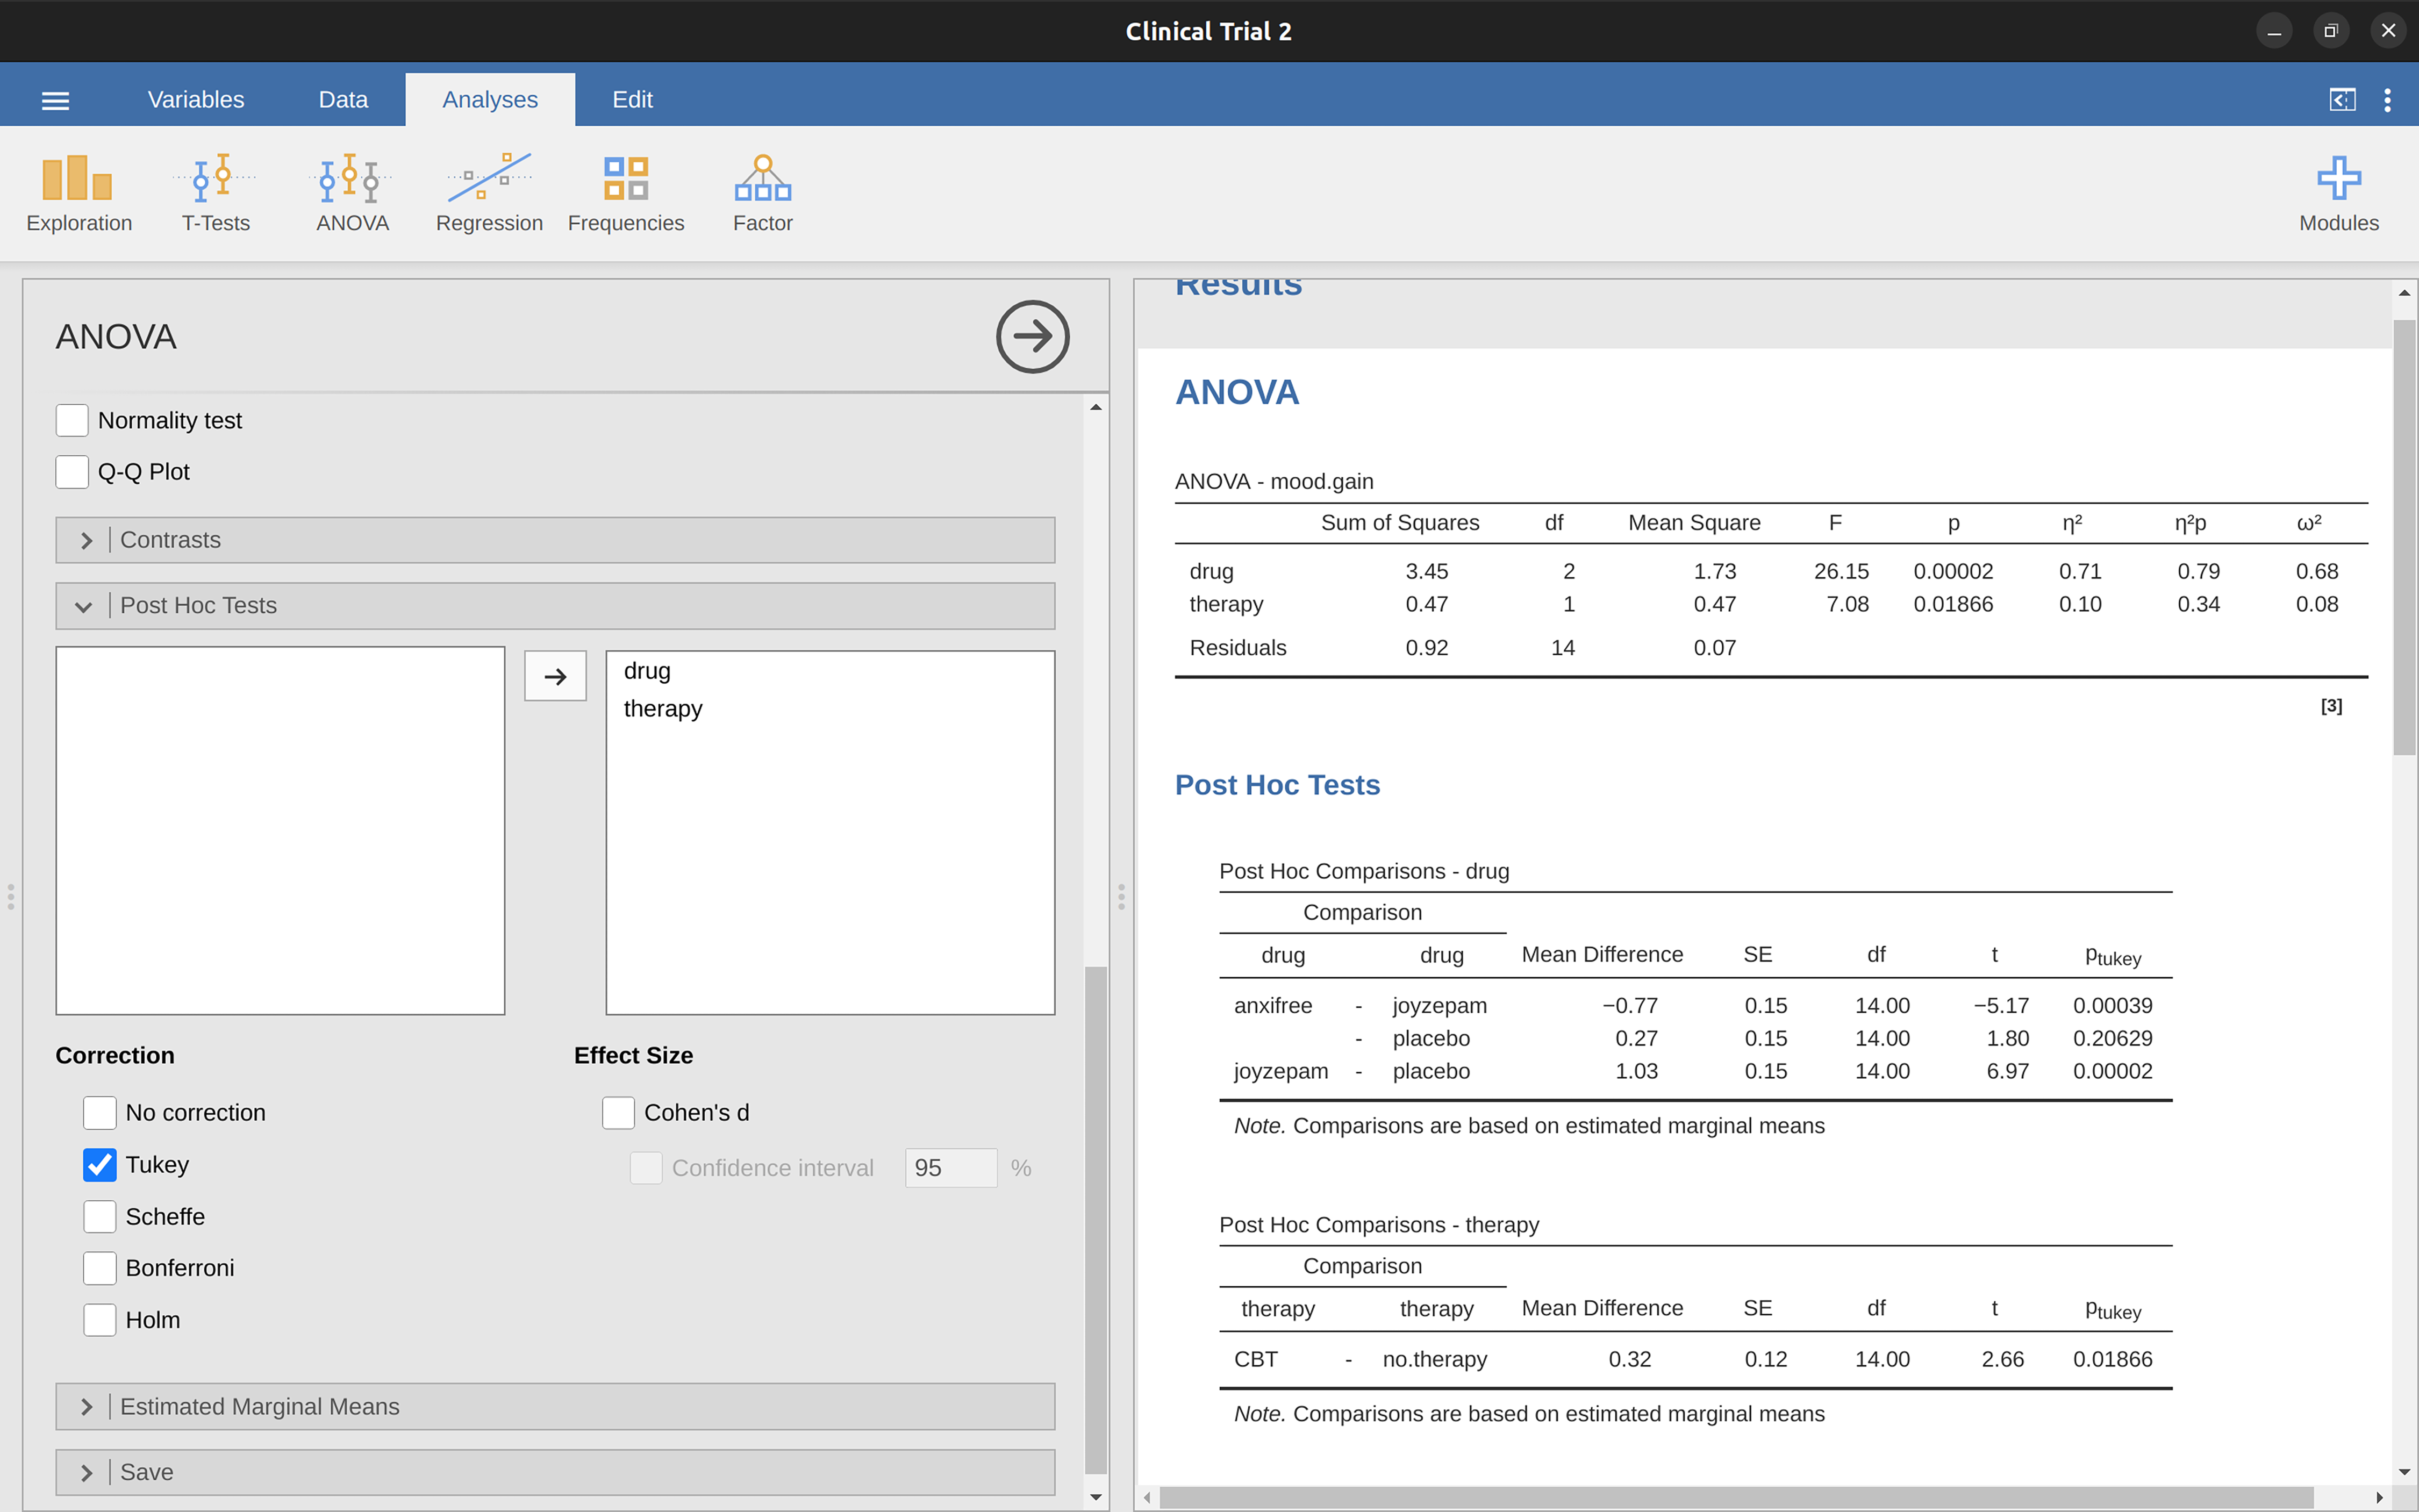
\includegraphics[width=1\textwidth,height=\textheight]{images/fig14-24.png} \hfill{}

\caption{\label{fig-fig14-24}Tukey HSD post hoc test in jamovi factorial
ANOVA, without an interaction term}

\end{figure}

The output shown in the `Post Hoc Tests' results table is (I hope)
pretty straightforward. The first comparison, for example, is the
Anxifree versus placebo difference, and the first part of the output
indicates that the observed difference in group means is .27. The next
number is the standard error for the difference, from which we could
calculate the 95\% confidence interval if we wanted, though jamovi does
not currently provide this option. Then there is a column with the
degrees of freedom, a column with the \(t\)-value, and finally a column
with the \(p\)-value. For the first comparison the adjusted \(p\)-value
is .21. In contrast, if you look at the next line, we see that the
observed difference between joyzepam and the placebo is 1.03, and this
result is significant (\(p < .001\)).

So far, so good. What about the situation where your model includes
interaction terms? For instance, the default option in jamovi is to
allow for the possibility that there is an interaction between drug and
therapy. If that's the case, the number of pairwise comparisons that we
need to consider starts to increase. As before, we need to consider the
three comparisons that are relevant to the main effect of drug and the
one comparison that is relevant to the main effect of therapy. But, if
we want to consider the possibility of a significant interaction (and
try to find the group differences that underpin that significant
interaction), we need to include comparisons such as the following:

\begin{itemize}
\tightlist
\item
  The difference in mood gain for people given Anxifree and treated with
  CBT, versus people given the placebo and treated with CBT.
\item
  The difference in mood gain for people given Anxifree and given no
  therapy, versus people given the placebo and given no therapy.
\item
  etc.
\end{itemize}

There are quite a lot of these comparisons that you need to consider.
So, when we run the Tukey post hoc analysis for this ANOVA model, we see
that it has made a lot of pairwise comparisons (19 in total), as shown
in Figure~\ref{fig-fig14-25}. You can see that it looks pretty similar
to before, but with a lot more comparisons made.

\begin{figure}

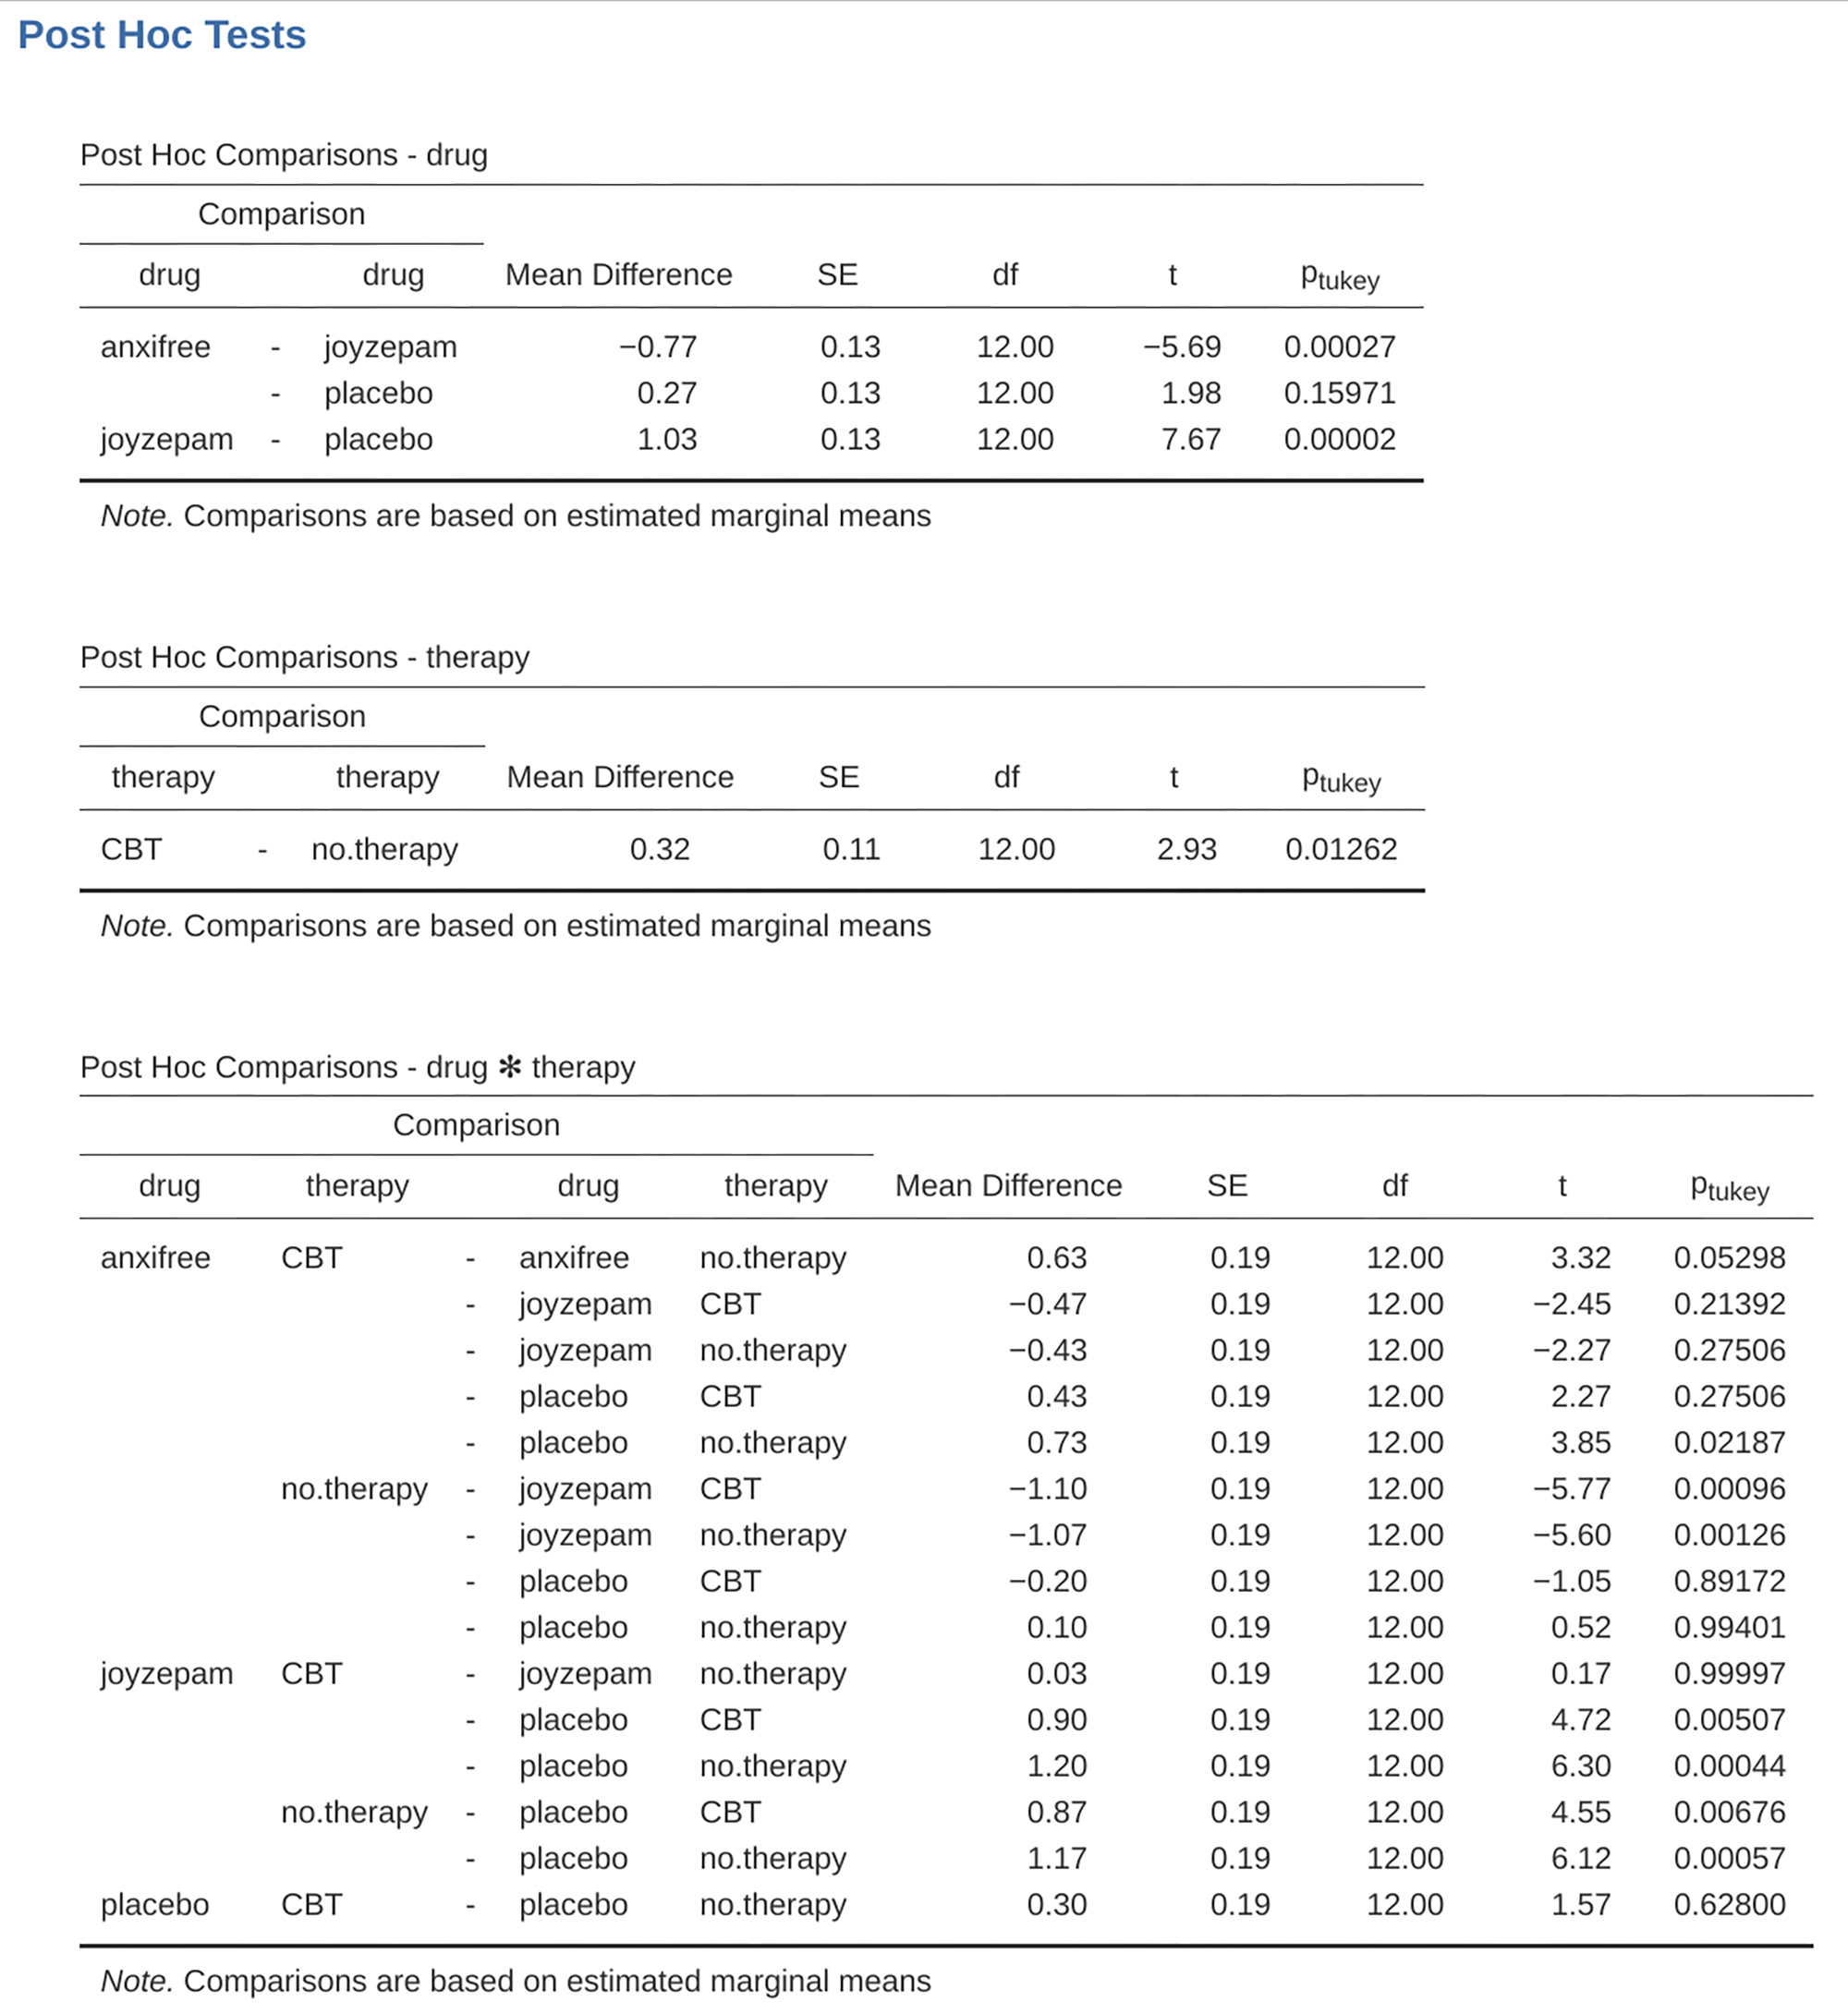
\includegraphics[width=1\textwidth,height=\textheight]{images/fig14-25.png} \hfill{}

\caption{\label{fig-fig14-25}Tukey HSD post hoc test in jamovi factorial
ANOVA with an interaction term}

\end{figure}

\hypertarget{sec-The-method-of-planned-comparisons}{%
\section{The method of planned
comparisons}\label{sec-The-method-of-planned-comparisons}}

Following on from the previous sections on contrasts and post hoc tests
in ANOVA, I think the method of planned comparisons is important enough
to deserve a quick discussion. In our discussions of multiple
comparisons, in the previous section and back in
\textbf{?@sec-Comparing-several-means-one-way-ANOVA}, I've been assuming
that the tests you want to run are genuinely post hoc. For instance, in
our drugs example above, maybe you thought that the drugs would all have
different effects on mood (i.e., you hypothesised a main effect of
drug), but you didn't have any specific hypothesis about how they would
be different, nor did you have any real idea about which pairwise
comparisons would be worth looking at. If that is the case, then you
really have to resort to something like Tukey's HSD to do your pairwise
comparisons.

The situation is rather different, however, if you genuinely did have
real, specific hypotheses about which comparisons are of interest, and
you never ever have any intention to look at any other comparisons
besides the ones that you specified ahead of time. When this is true,
and if you honestly and rigorously stick to your noble intentions to not
run any other comparisons (even when the data look like they're showing
you deliciously significant effects for stuff you didn't have a
hypothesis test for), then it doesn't really make a lot of sense to run
something like Tukey's HSD, because it makes corrections for a whole
bunch of comparisons that you never cared about and never had any
intention of looking at. Under those circumstances, you can safely run a
(limited) number of hypothesis tests without making an adjustment for
multiple testing. This situation is known as the method of planned
comparisons, and it is sometimes used in clinical trials. However,
further consideration is out of scope for this introductory book, but at
least you know that this method exists!

\hypertarget{factorial-anova-3-unbalanced-designs}{%
\section{Factorial ANOVA 3: unbalanced
designs}\label{factorial-anova-3-unbalanced-designs}}

Factorial ANOVA is a very handy thing to know about. It's been one of
the standard tools used to analyse experimental data for many decades,
and you'll find that you can't read more than two or three papers in
psychology without running into an ANOVA in there somewhere. However,
there's one huge difference between the ANOVAs that you'll see in a lot
of real scientific articles and the ANOVAs that I've described so far.
In in real life we're rarely lucky enough to have perfectly balanced
designs. For one reason or another, it's typical to end up with more
observations in some cells than in others. Or, to put it another way, we
have an unbalanced design.

Unbalanced designs need to be treated with a lot more care than balanced
designs, and the statistical theory that underpins them is a lot
messier. It might be a consequence of this messiness, or it might be a
shortage of time, but my experience has been that undergraduate research
methods classes in psychology have a nasty tendency to ignore this issue
completely. A lot of stats textbooks tend to gloss over it too. The net
result of this, I think, is that a lot of active researchers in the
field don't actually know that there's several different ``types'' of
unbalanced ANOVAs, and they produce quite different answers. In fact,
reading the psychological literature, I'm kind of amazed at the fact
that most people who report the results of an unbalanced factorial ANOVA
don't actually give you enough details to reproduce the analysis. I
secretly suspect that most people don't even realise that their
statistical software package is making a whole lot of substantive data
analysis decisions on their behalf. It's actually a little terrifying
when you think about it. So, if you want to avoid handing control of
your data analysis to stupid software, read on.

\hypertarget{the-coffee-data}{%
\subsection{\texorpdfstring{The \emph{coffee}
data}{The coffee data}}\label{the-coffee-data}}

As usual, it will help us to work with some data. The \emph{coffee.csv}
file contains a hypothetical data set that produces an unbalanced
\(3 \times 2\) ANOVA. Suppose we were interested in finding out whether
or not the tendency of people to babble when they have too much coffee
is purely an effect of the coffee itself, or whether there's some effect
of the milk and sugar that people add to the coffee. Suppose we took 18
people and gave them some coffee to drink. The amount of coffee /
caffeine was held constant, and we varied whether or not milk was added,
so milk is a binary factor with two levels, ``yes'' and ``no''. We also
varied the kind of sugar involved. The coffee might contain ``real''
sugar or it might contain ``fake'' sugar (i.e., artificial sweetener) or
it might contain ``none'' at all, so the sugar variable is a three level
factor. Our outcome variable is a continuous variable that presumably
refers to some psychologically sensible measure of the extent to which
someone is ``babbling''. The details don't really matter for our
purpose. Take a look at the data in the jamovi spreadsheet view, as in
Figure~\ref{fig-fig14-26}.

\begin{figure}

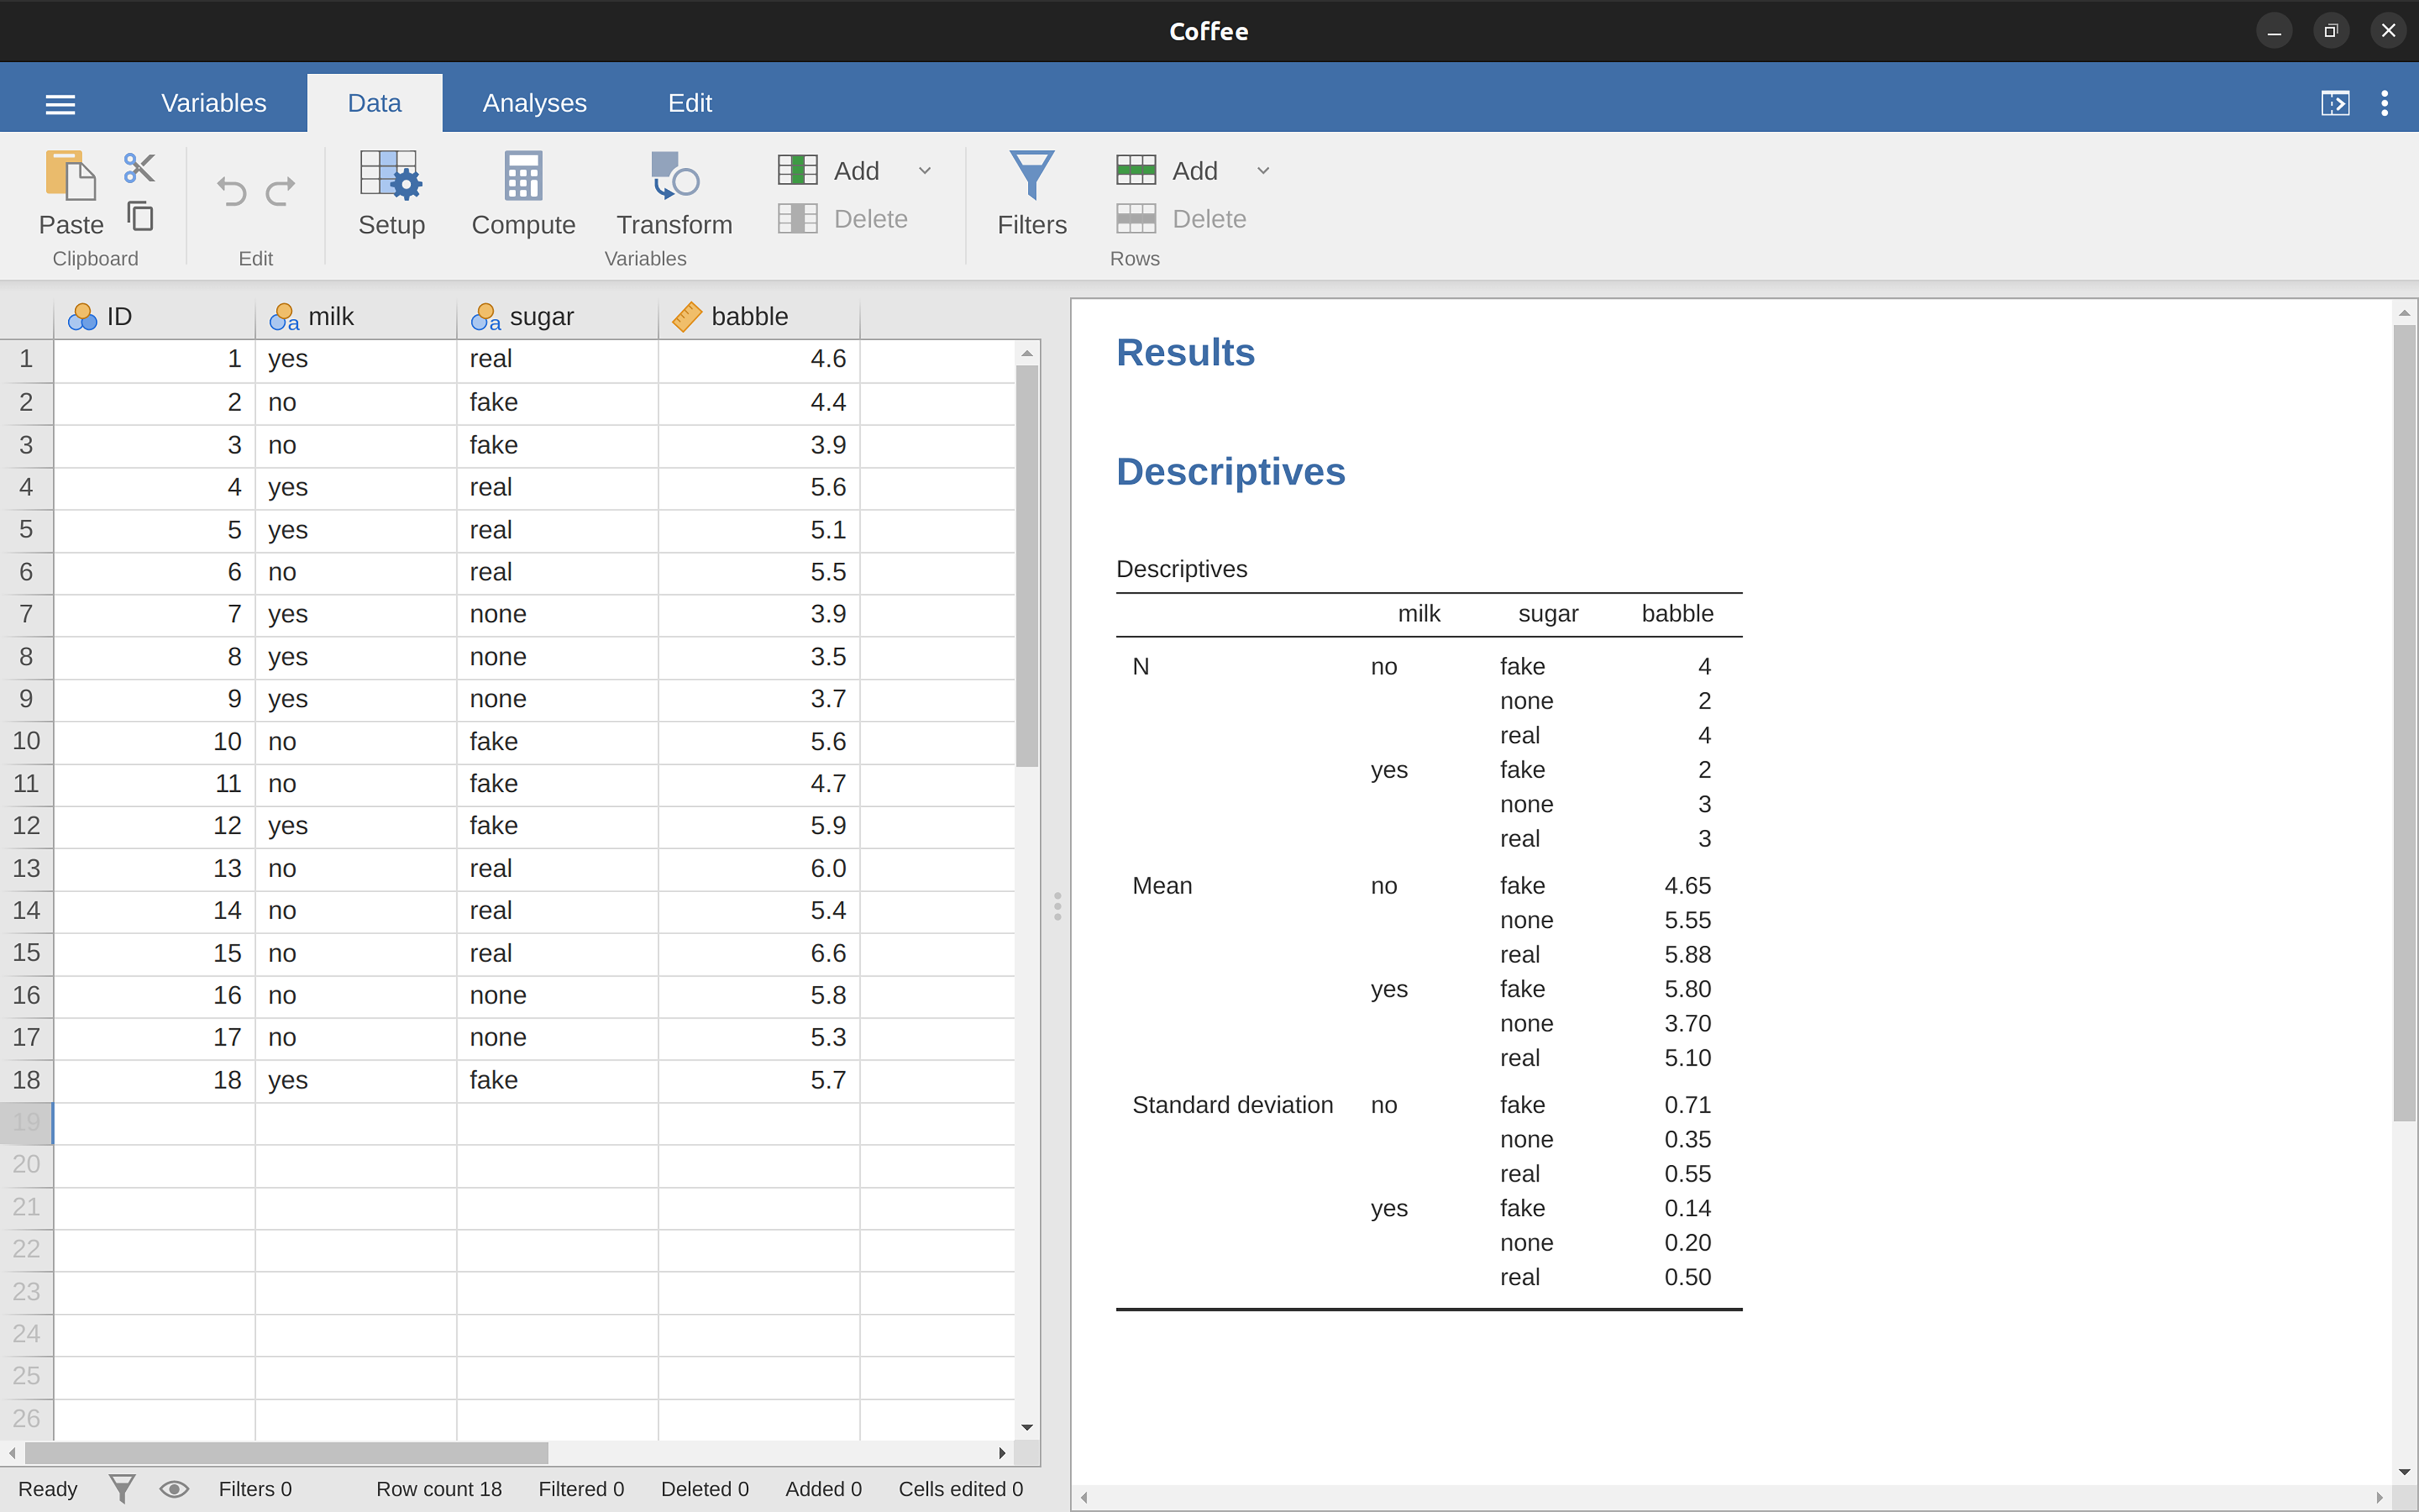
\includegraphics[width=1\textwidth,height=\textheight]{images/fig14-26.png} \hfill{}

\caption{\label{fig-fig14-26}The \emph{coffee.csv} data set in jamovi,
with descriptive information aggregated by factor levels}

\end{figure}

Looking at the table of means in Figure~\ref{fig-fig14-26} we get a
strong impression that there are differences between the groups. This is
especially true when we compare these means to the standard deviations
for the babble variable. Across groups, this standard deviation varies
from .14 to .71, which is fairly small relative to the differences in
group means.\footnote{This discrepancy in standard deviations might (and
  should) make you wonder if we have a violation of the homogeneity of
  variance assumption. I'll leave it as an exercise for the reader to
  double check this using the Levene test option.} Whilst this at first
may seem like a straightforward factorial ANOVA, a problem arises when
we look at how many observations we have in each group. See the
different \(N\)s for different groups shown in
Figure~\ref{fig-fig14-26}. This violates one of our original
assumptions, namely that the number of people in each group is the same.
We haven't really discussed how to handle this situation.

\hypertarget{standard-anova-does-not-exist-for-unbalanced-designs}{%
\subsection{``Standard ANOVA'' does not exist for unbalanced
designs}\label{standard-anova-does-not-exist-for-unbalanced-designs}}

Unbalanced designs lead us to the somewhat unsettling discovery that
there isn't really any one thing that we might refer to as a standard
ANOVA. In fact, it turns out that there are three fundamentally
different ways\footnote{Actually, this is a bit of a lie. ANOVAs can
  vary in other ways besides the ones I've discussed in this book. For
  instance, I've completely ignored the difference between fixed-effect
  models in which the levels of a factor are ``fixed'' by the
  experimenter or the world, and random-effect models in which the
  levels are random samples from a larger population of possible levels
  (this book only covers fixed-effect models). Don't make the mistake of
  thinking that this book, or any other one, will tell you ``everything
  you need to know'' about statistics, any more than a single book could
  possibly tell you everything you need to know about psychology,
  physics or philosophy. Life is too complicated for that to ever be
  true. This isn't a cause for despair, though. Most researchers get by
  with a basic working knowledge of ANOVA that doesn't go any further
  than this book does. I just want you to keep in mind that this book is
  only the beginning of a very long story, not the whole story.} in
which you might want to run an ANOVA in an unbalanced design. If you
have a balanced design all three versions produce identical results,
with the sums of squares, \(F\)-values, etc., all conforming to the
formulas that I gave at the start of the chapter. However, when your
design is unbalanced they don't give the same answers. Furthermore, they
are not all equally appropriate to every situation. Some methods will be
more appropriate to your situation than others. Given all this, it's
important to understand what the different types of ANOVA are and how
they differ from one another.

The first kind of ANOVA is conventionally referred to as \textbf{type I
sum of squares}. I'm sure you can guess what the other two are called.
The ``sum of squares'' part of the name was introduced by the SAS
statistical software package and has become standard nomenclature, but
it's a bit misleading in some ways. I think the logic for referring to
them as different types of sum of squares is that, when you look at the
ANOVA tables that they produce, the key difference in the numbers is the
\(SS\) values. The degrees of freedom don't change, the \(MS\) values
are still defined as \(SS\) divided by \(df\), etc. However, what the
terminology gets wrong is that it hides the reason \emph{why} the \(SS\)
values are different from one another. To that end, it's a lot more
helpful to think of the three different kinds of ANOVA as three
different \emph{hypothesis testing strategies}. These different
strategies lead to different \(SS\) values, to be sure, but it's the
strategy that is the important thing here, not the \(SS\) values
themselves. Recall from the section
\protect\hyperlink{sec-ANOVA-as-a-linear-model}{ANOVA as a linear model}
that any particular \(F\)-test is best thought of as a comparison
between two linear models. So, when you're looking at an ANOVA table, it
helps to remember that each of those \(F\)-tests corresponds to a pair
of models that are being compared. Of course, this leads naturally to
the question of which pair of models is being compared. This is the
fundamental difference between ANOVA types I, II and III: each one
corresponds to a different way of choosing the model pairs for the
tests.

\hypertarget{type-i-sum-of-squares}{%
\subsection{Type I sum of squares}\label{type-i-sum-of-squares}}

The type I method is sometimes referred to as the ``sequential'' sum of
squares, because it involves a process of adding terms to the model one
at a time. Consider the \emph{coffee} data, for instance. Suppose we
want to run the full \(3 \times 2\) factorial ANOVA, including
interaction terms. The full model contains the outcome variable babble,
the predictor variables sugar and milk, and the interaction term sugar
\(\times\) milk. This can be written as
\(babble \sim sugar + milk + sugar {\times} milk\). The type I strategy
builds this model up sequentially, starting from the simplest possible
model and gradually adding terms.

The simplest possible model for the data would be one in which neither
milk nor sugar is assumed to have any effect on babbling. The only term
that would be included in such a model is the intercept, written as
babble \textasciitilde{} 1. This is our initial null hypothesis. The
next simplest model for the data would be one in which only one of the
two main effects is included. In the \emph{coffee} data, there are two
different possible choices here, because we could choose to add milk
first or to add sugar first. The order actually turns out to matter, as
we'll see later, but for now let's just make a choice arbitrarily and
pick sugar. So, the second model in our sequence of models is babble
\textasciitilde{} sugar, and it forms the alternative hypothesis for our
first test. We now have our first hypothesis test
(Table~\ref{tbl-tab14-16}).

\hypertarget{tbl-tab14-16}{}
 
  \providecommand{\huxb}[2]{\arrayrulecolor[RGB]{#1}\global\arrayrulewidth=#2pt}
  \providecommand{\huxvb}[2]{\color[RGB]{#1}\vrule width #2pt}
  \providecommand{\huxtpad}[1]{\rule{0pt}{#1}}
  \providecommand{\huxbpad}[1]{\rule[-#1]{0pt}{#1}}

\begin{table}[ht]
\caption{\label{tbl-tab14-16}Null and alternative hypotheses with the outcome variable ``babble'' }\tabularnewline

\begin{centerbox}
\begin{threeparttable}
\setlength{\tabcolsep}{0pt}
\begin{tabularx}{0.9\textwidth}{p{0.45\textwidth} p{0.45\textwidth}}


\hhline{>{\huxb{0, 0, 0}{0.4}}->{\huxb{0, 0, 0}{0.4}}-}
\arrayrulecolor{black}

\multicolumn{1}{!{\huxvb{0, 0, 0}{0}}p{0.45\textwidth}!{\huxvb{0, 0, 0}{0}}}{\hspace{0pt}\parbox[b]{0.45\textwidth-0pt-12pt}{\huxtpad{2pt + 1em}\centering \textbf{Null model:}\huxbpad{2pt}}} &
\multicolumn{1}{p{0.45\textwidth}!{\huxvb{0, 0, 0}{0}}}{\hspace{12pt}\parbox[b]{0.45\textwidth-12pt-0pt}{\huxtpad{2pt + 1em}\centering \textbf{\(babble \sim 1\)}\huxbpad{2pt}}} \tabularnewline[-0.5pt]


\hhline{>{\huxb{0, 0, 0}{0.4}}->{\huxb{0, 0, 0}{0.4}}-}
\arrayrulecolor{black}

\multicolumn{1}{!{\huxvb{0, 0, 0}{0}}p{0.45\textwidth}!{\huxvb{0, 0, 0}{0}}}{\hspace{0pt}\parbox[b]{0.45\textwidth-0pt-12pt}{\huxtpad{2pt + 1em}\centering Alternative model:\huxbpad{2pt}}} &
\multicolumn{1}{p{0.45\textwidth}!{\huxvb{0, 0, 0}{0}}}{\hspace{12pt}\parbox[b]{0.45\textwidth-12pt-0pt}{\huxtpad{2pt + 1em}\centering \(babble \sim  sugar\)\huxbpad{2pt}}} \tabularnewline[-0.5pt]


\hhline{>{\huxb{0, 0, 0}{0.4}}->{\huxb{0, 0, 0}{0.4}}-}
\arrayrulecolor{black}
\end{tabularx} 

\end{threeparttable}\par\end{centerbox}

\end{table}
 

This comparison forms our hypothesis test of the main effect of sugar.
The next step in our model building exercise is to add the other main
effect term, so the next model in our sequence is babble
\textasciitilde{} sugar + milk. The second hypothesis test is then
formed by comparing the following pair of models
(Table~\ref{tbl-tab14-17}).

\hypertarget{tbl-tab14-17}{}
 
  \providecommand{\huxb}[2]{\arrayrulecolor[RGB]{#1}\global\arrayrulewidth=#2pt}
  \providecommand{\huxvb}[2]{\color[RGB]{#1}\vrule width #2pt}
  \providecommand{\huxtpad}[1]{\rule{0pt}{#1}}
  \providecommand{\huxbpad}[1]{\rule[-#1]{0pt}{#1}}

\begin{table}[ht]
\caption{\label{tbl-tab14-17}Further null and alternative hypotheses with the outcome variable
``babble'' }\tabularnewline

\begin{centerbox}
\begin{threeparttable}
\setlength{\tabcolsep}{0pt}
\begin{tabularx}{0.9\textwidth}{p{0.45\textwidth} p{0.45\textwidth}}


\hhline{>{\huxb{0, 0, 0}{0.4}}->{\huxb{0, 0, 0}{0.4}}-}
\arrayrulecolor{black}

\multicolumn{1}{!{\huxvb{0, 0, 0}{0}}p{0.45\textwidth}!{\huxvb{0, 0, 0}{0}}}{\hspace{0pt}\parbox[b]{0.45\textwidth-0pt-12pt}{\huxtpad{2pt + 1em}\centering \textbf{Null model:}\huxbpad{2pt}}} &
\multicolumn{1}{p{0.45\textwidth}!{\huxvb{0, 0, 0}{0}}}{\hspace{12pt}\parbox[b]{0.45\textwidth-12pt-0pt}{\huxtpad{2pt + 1em}\centering \textbf{\(babble \sim  sugar\)}\huxbpad{2pt}}} \tabularnewline[-0.5pt]


\hhline{>{\huxb{0, 0, 0}{0.4}}->{\huxb{0, 0, 0}{0.4}}-}
\arrayrulecolor{black}

\multicolumn{1}{!{\huxvb{0, 0, 0}{0}}p{0.45\textwidth}!{\huxvb{0, 0, 0}{0}}}{\hspace{0pt}\parbox[b]{0.45\textwidth-0pt-12pt}{\huxtpad{2pt + 1em}\centering Alternative model:\huxbpad{2pt}}} &
\multicolumn{1}{p{0.45\textwidth}!{\huxvb{0, 0, 0}{0}}}{\hspace{12pt}\parbox[b]{0.45\textwidth-12pt-0pt}{\huxtpad{2pt + 1em}\centering \(babble \sim  sugar + milk\)\huxbpad{2pt}}} \tabularnewline[-0.5pt]


\hhline{>{\huxb{0, 0, 0}{0.4}}->{\huxb{0, 0, 0}{0.4}}-}
\arrayrulecolor{black}
\end{tabularx} 

\end{threeparttable}\par\end{centerbox}

\end{table}
 

This comparison forms our hypothesis test of the main effect of milk. In
one sense, this approach is very elegant: the alternative hypothesis
from the first test forms the null hypothesis for the second one. It is
in this sense that the type I method is strictly sequential. Every test
builds directly on the results of the last one. However, in another
sense it's very inelegant, because there's a strong asymmetry between
the two tests. The test of the main effect of sugar (the first test)
completely ignores milk, whereas the test of the main effect of milk
(the second test) does take sugar into account. In any case, the fourth
model in our sequence is now the full model, babble \textasciitilde{}
sugar + milk + sugar \(\times\) milk, and the corresponding hypothesis
test is shown in Table~\ref{tbl-tab14-18}.

\hypertarget{tbl-tab14-18}{}
 
  \providecommand{\huxb}[2]{\arrayrulecolor[RGB]{#1}\global\arrayrulewidth=#2pt}
  \providecommand{\huxvb}[2]{\color[RGB]{#1}\vrule width #2pt}
  \providecommand{\huxtpad}[1]{\rule{0pt}{#1}}
  \providecommand{\huxbpad}[1]{\rule[-#1]{0pt}{#1}}

\begin{table}[ht]
\caption{\label{tbl-tab14-18}And more possible null and alternative hypotheses with the outcome
variable ``babble'' }\tabularnewline

\begin{centerbox}
\begin{threeparttable}
\setlength{\tabcolsep}{0pt}
\begin{tabularx}{0.9\textwidth}{p{0.45\textwidth} p{0.45\textwidth}}


\hhline{>{\huxb{0, 0, 0}{0.4}}->{\huxb{0, 0, 0}{0.4}}-}
\arrayrulecolor{black}

\multicolumn{1}{!{\huxvb{0, 0, 0}{0}}p{0.45\textwidth}!{\huxvb{0, 0, 0}{0}}}{\hspace{0pt}\parbox[b]{0.45\textwidth-0pt-12pt}{\huxtpad{2pt + 1em}\centering \textbf{Null model:}\huxbpad{2pt}}} &
\multicolumn{1}{p{0.45\textwidth}!{\huxvb{0, 0, 0}{0}}}{\hspace{12pt}\parbox[b]{0.45\textwidth-12pt-0pt}{\huxtpad{2pt + 1em}\centering \textbf{\(babble \sim  sugar + milk\)}\huxbpad{2pt}}} \tabularnewline[-0.5pt]


\hhline{>{\huxb{0, 0, 0}{0.4}}->{\huxb{0, 0, 0}{0.4}}-}
\arrayrulecolor{black}

\multicolumn{1}{!{\huxvb{0, 0, 0}{0}}p{0.45\textwidth}!{\huxvb{0, 0, 0}{0}}}{\hspace{0pt}\parbox[b]{0.45\textwidth-0pt-12pt}{\huxtpad{2pt + 1em}\centering Alternative model:\huxbpad{2pt}}} &
\multicolumn{1}{p{0.45\textwidth}!{\huxvb{0, 0, 0}{0}}}{\hspace{12pt}\parbox[b]{0.45\textwidth-12pt-0pt}{\huxtpad{2pt + 1em}\centering \(babble \sim  sugar + milk + sugar * milk \)\huxbpad{2pt}}} \tabularnewline[-0.5pt]


\hhline{>{\huxb{0, 0, 0}{0.4}}->{\huxb{0, 0, 0}{0.4}}-}
\arrayrulecolor{black}
\end{tabularx} 

\end{threeparttable}\par\end{centerbox}

\end{table}
 

Type III sum of squares is the default hypothesis testing method used by
jamovi ANOVA, so to run a type I sum of squares analysis we have to
select `Type 1' in the `Sum of squares' selection box in the jamovi
`ANOVA' - `Model' options. This gives us the ANOVA table shown in
Figure~\ref{fig-fig14-27}.

\begin{figure}

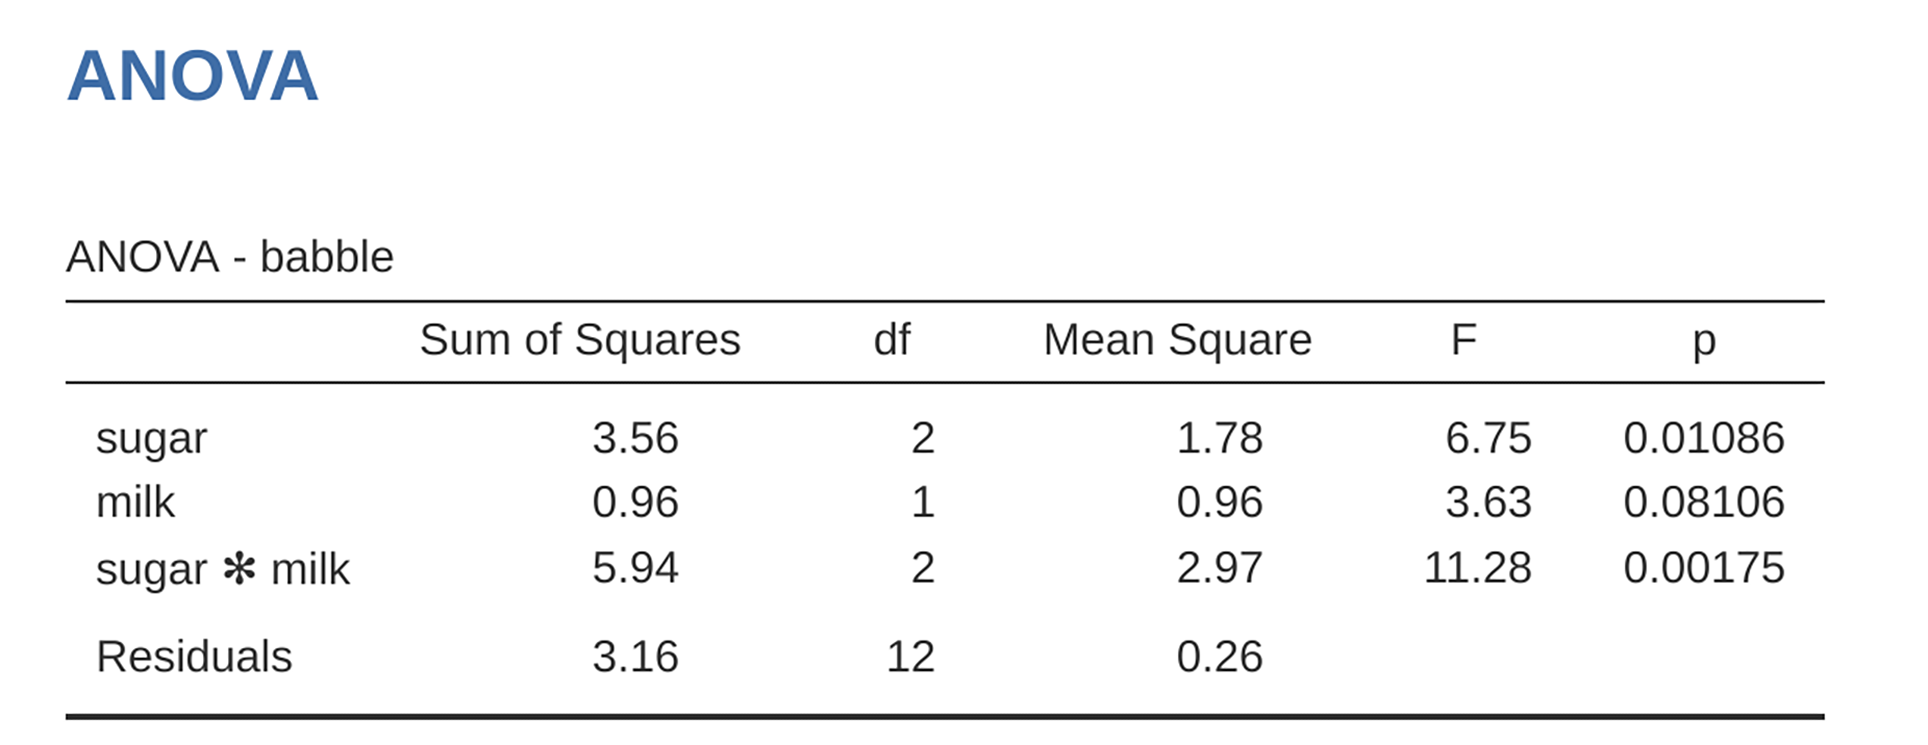
\includegraphics[width=1\textwidth,height=\textheight]{images/fig14-27.png} \hfill{}

\caption{\label{fig-fig14-27}ANOVA results table using type I sum of
squares in jamovi}

\end{figure}

The big problem with using type I sum of squares is the fact that it
really does depend on the order in which you enter the variables. Yet,
in many situations the researcher has no reason to prefer one ordering
over another. This is presumably the case for our milk and sugar
problem. Should we add milk first or sugar first? It feels exactly as
arbitrary as a data analysis question as it does as a coffee-making
question. There may in fact be some people with firm opinions about
ordering, but it's hard to imagine a principled answer to the question.
Yet, look what happens when we change the ordering, as in
Figure~\ref{fig-fig14-28}.

\begin{figure}

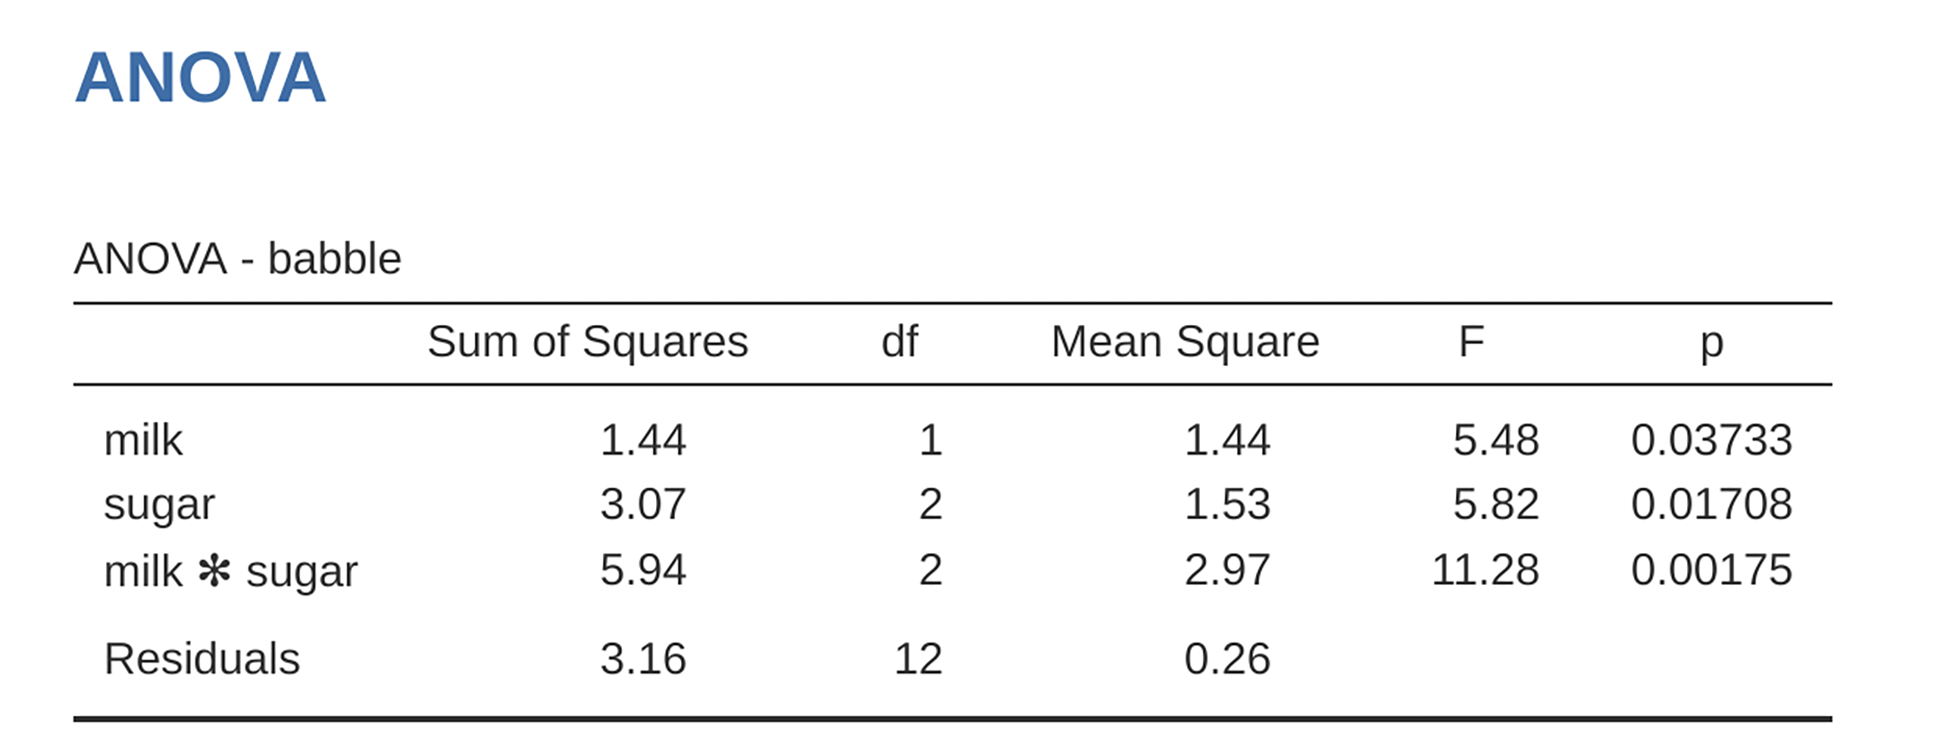
\includegraphics[width=1\textwidth,height=\textheight]{images/fig14-28.png} \hfill{}

\caption{\label{fig-fig14-28}ANOVA results table using type I sum of
squares in jamovi, but with factors entered in a different order (milk
first)}

\end{figure}

The \(p\)-values for both main effect terms have changed, and fairly
dramatically. Among other things, the effect of milk has become
significant (though one should avoid drawing any strong conclusions
about this, as I've mentioned previously). Which of these two ANOVAs
should one report? It's not immediately obvious.

When you look at the hypothesis tests that are used to define the
``first'' main effect and the ``second'' one, it's clear that they're
qualitatively different from one another. In our initial example, we saw
that the test for the main effect of sugar completely ignores milk,
whereas the test of the main effect of milk does take sugar into
account. As such, the type I testing strategy really does treat the
first main effect as if it had a kind of theoretical primacy over the
second one. In my experience there is very rarely if ever any
theoretically primacy of this kind that would justify treating any two
main effects asymmetrically.

The consequence of all this is that type I tests are very rarely of much
interest, and so we should move on to discuss type II tests and type III
tests.

\hypertarget{type-iii-sum-of-squares}{%
\subsection{Type III sum of squares}\label{type-iii-sum-of-squares}}

Having just finished talking about type I tests, you might think that
the natural thing to do next would be to talk about type II tests.
However, I think it's actually a bit more natural to discuss type III
tests (which are simple and the default in jamovi ANOVA) before talking
about type II tests (which are trickier). The basic idea behind type III
tests is extremely simple. Regardless of which term you're trying to
evaluate, run the \(F\)-test in which the alternative hypothesis
corresponds to the full ANOVA model as specified by the user, and the
null model just deletes that one term that you're testing. For instance,
in the coffee example, in which our full model was babble
\textasciitilde{} sugar + milk + sugar \(\times\) milk, the test for a
main effect of sugar would correspond to a comparison between the
following two models (Table~\ref{tbl-tab14-19}).

\hypertarget{tbl-tab14-19}{}
 
  \providecommand{\huxb}[2]{\arrayrulecolor[RGB]{#1}\global\arrayrulewidth=#2pt}
  \providecommand{\huxvb}[2]{\color[RGB]{#1}\vrule width #2pt}
  \providecommand{\huxtpad}[1]{\rule{0pt}{#1}}
  \providecommand{\huxbpad}[1]{\rule[-#1]{0pt}{#1}}

\begin{table}[ht]
\caption{\label{tbl-tab14-19}Null and alternative hypotheses with the outcome variable ``babble'',
with type III sum of squares }\tabularnewline

\begin{centerbox}
\begin{threeparttable}
\setlength{\tabcolsep}{0pt}
\begin{tabularx}{0.9\textwidth}{p{0.45\textwidth} p{0.45\textwidth}}


\hhline{>{\huxb{0, 0, 0}{0.4}}->{\huxb{0, 0, 0}{0.4}}-}
\arrayrulecolor{black}

\multicolumn{1}{!{\huxvb{0, 0, 0}{0}}p{0.45\textwidth}!{\huxvb{0, 0, 0}{0}}}{\hspace{0pt}\parbox[b]{0.45\textwidth-0pt-12pt}{\huxtpad{2pt + 1em}\centering \textbf{Null model:}\huxbpad{2pt}}} &
\multicolumn{1}{p{0.45\textwidth}!{\huxvb{0, 0, 0}{0}}}{\hspace{12pt}\parbox[b]{0.45\textwidth-12pt-0pt}{\huxtpad{2pt + 1em}\centering \textbf{\(babble \sim  milk + sugar * milk\)}\huxbpad{2pt}}} \tabularnewline[-0.5pt]


\hhline{>{\huxb{0, 0, 0}{0.4}}->{\huxb{0, 0, 0}{0.4}}-}
\arrayrulecolor{black}

\multicolumn{1}{!{\huxvb{0, 0, 0}{0}}p{0.45\textwidth}!{\huxvb{0, 0, 0}{0}}}{\hspace{0pt}\parbox[b]{0.45\textwidth-0pt-12pt}{\huxtpad{2pt + 1em}\centering Alternative model:\huxbpad{2pt}}} &
\multicolumn{1}{p{0.45\textwidth}!{\huxvb{0, 0, 0}{0}}}{\hspace{12pt}\parbox[b]{0.45\textwidth-12pt-0pt}{\huxtpad{2pt + 1em}\centering \(babble \sim  sugar + milk +sugar * milk \)\huxbpad{2pt}}} \tabularnewline[-0.5pt]


\hhline{>{\huxb{0, 0, 0}{0.4}}->{\huxb{0, 0, 0}{0.4}}-}
\arrayrulecolor{black}
\end{tabularx} 

\end{threeparttable}\par\end{centerbox}

\end{table}
 

Similarly the main effect of milk is evaluated by testing the full model
against a null model that removes the milk term, like in
Table~\ref{tbl-tab14-20}.

\hypertarget{tbl-tab14-20}{}
 
  \providecommand{\huxb}[2]{\arrayrulecolor[RGB]{#1}\global\arrayrulewidth=#2pt}
  \providecommand{\huxvb}[2]{\color[RGB]{#1}\vrule width #2pt}
  \providecommand{\huxtpad}[1]{\rule{0pt}{#1}}
  \providecommand{\huxbpad}[1]{\rule[-#1]{0pt}{#1}}

\begin{table}[ht]
\caption{\label{tbl-tab14-20}Further null and alternative hypotheses with the outcome variable
`babble', with type III sum of squares }\tabularnewline

\begin{centerbox}
\begin{threeparttable}
\setlength{\tabcolsep}{0pt}
\begin{tabularx}{0.9\textwidth}{p{0.45\textwidth} p{0.45\textwidth}}


\hhline{>{\huxb{0, 0, 0}{0.4}}->{\huxb{0, 0, 0}{0.4}}-}
\arrayrulecolor{black}

\multicolumn{1}{!{\huxvb{0, 0, 0}{0}}p{0.45\textwidth}!{\huxvb{0, 0, 0}{0}}}{\hspace{0pt}\parbox[b]{0.45\textwidth-0pt-12pt}{\huxtpad{2pt + 1em}\centering \textbf{Null model:}\huxbpad{2pt}}} &
\multicolumn{1}{p{0.45\textwidth}!{\huxvb{0, 0, 0}{0}}}{\hspace{12pt}\parbox[b]{0.45\textwidth-12pt-0pt}{\huxtpad{2pt + 1em}\centering \textbf{\(babble \sim  sugar + sugar * milk\)}\huxbpad{2pt}}} \tabularnewline[-0.5pt]


\hhline{>{\huxb{0, 0, 0}{0.4}}->{\huxb{0, 0, 0}{0.4}}-}
\arrayrulecolor{black}

\multicolumn{1}{!{\huxvb{0, 0, 0}{0}}p{0.45\textwidth}!{\huxvb{0, 0, 0}{0}}}{\hspace{0pt}\parbox[b]{0.45\textwidth-0pt-12pt}{\huxtpad{2pt + 1em}\centering Alternative model:\huxbpad{2pt}}} &
\multicolumn{1}{p{0.45\textwidth}!{\huxvb{0, 0, 0}{0}}}{\hspace{12pt}\parbox[b]{0.45\textwidth-12pt-0pt}{\huxtpad{2pt + 1em}\centering \(babble \sim  sugar + milk +sugar * milk \)\huxbpad{2pt}}} \tabularnewline[-0.5pt]


\hhline{>{\huxb{0, 0, 0}{0.4}}->{\huxb{0, 0, 0}{0.4}}-}
\arrayrulecolor{black}
\end{tabularx} 

\end{threeparttable}\par\end{centerbox}

\end{table}
 

Finally, the interaction term sugar \(\times\) milk is evaluated in
exactly the same way. Once again, we test the full model against a null
model that removes the sugar \(\times\) milk interaction term, like in
Table~\ref{tbl-tab14-21}.

\hypertarget{tbl-tab14-21}{}
 
  \providecommand{\huxb}[2]{\arrayrulecolor[RGB]{#1}\global\arrayrulewidth=#2pt}
  \providecommand{\huxvb}[2]{\color[RGB]{#1}\vrule width #2pt}
  \providecommand{\huxtpad}[1]{\rule{0pt}{#1}}
  \providecommand{\huxbpad}[1]{\rule[-#1]{0pt}{#1}}

\begin{table}[ht]
\caption{\label{tbl-tab14-21}Removing the interaction term from hypotheses with the outcome variable
`babble', with type III sum of squares }\tabularnewline

\begin{centerbox}
\begin{threeparttable}
\setlength{\tabcolsep}{0pt}
\begin{tabularx}{0.9\textwidth}{p{0.45\textwidth} p{0.45\textwidth}}


\hhline{>{\huxb{0, 0, 0}{0.4}}->{\huxb{0, 0, 0}{0.4}}-}
\arrayrulecolor{black}

\multicolumn{1}{!{\huxvb{0, 0, 0}{0}}p{0.45\textwidth}!{\huxvb{0, 0, 0}{0}}}{\hspace{0pt}\parbox[b]{0.45\textwidth-0pt-12pt}{\huxtpad{2pt + 1em}\centering \textbf{Null model:}\huxbpad{2pt}}} &
\multicolumn{1}{p{0.45\textwidth}!{\huxvb{0, 0, 0}{0}}}{\hspace{12pt}\parbox[b]{0.45\textwidth-12pt-0pt}{\huxtpad{2pt + 1em}\centering \textbf{\(babble \sim  sugar + milk\)}\huxbpad{2pt}}} \tabularnewline[-0.5pt]


\hhline{>{\huxb{0, 0, 0}{0.4}}->{\huxb{0, 0, 0}{0.4}}-}
\arrayrulecolor{black}

\multicolumn{1}{!{\huxvb{0, 0, 0}{0}}p{0.45\textwidth}!{\huxvb{0, 0, 0}{0}}}{\hspace{0pt}\parbox[b]{0.45\textwidth-0pt-12pt}{\huxtpad{2pt + 1em}\centering Alternative model:\huxbpad{2pt}}} &
\multicolumn{1}{p{0.45\textwidth}!{\huxvb{0, 0, 0}{0}}}{\hspace{12pt}\parbox[b]{0.45\textwidth-12pt-0pt}{\huxtpad{2pt + 1em}\centering \(babble \sim  sugar + milk +sugar * milk \)\huxbpad{2pt}}} \tabularnewline[-0.5pt]


\hhline{>{\huxb{0, 0, 0}{0.4}}->{\huxb{0, 0, 0}{0.4}}-}
\arrayrulecolor{black}
\end{tabularx} 

\end{threeparttable}\par\end{centerbox}

\end{table}
 

The basic idea generalises to higher order ANOVAs. For instance, suppose
that we were trying to run an ANOVA with three factors, A, B and C, and
we wanted to consider all possible main effects and all possible
interactions, including the three way interaction A \(\times\) B
\(\times\) C. (Table~\ref{tbl-tab14-22}) shows you what the Type III
tests look like for this situation).

\hypertarget{tbl-tab14-22}{}
 
  \providecommand{\huxb}[2]{\arrayrulecolor[RGB]{#1}\global\arrayrulewidth=#2pt}
  \providecommand{\huxvb}[2]{\color[RGB]{#1}\vrule width #2pt}
  \providecommand{\huxtpad}[1]{\rule{0pt}{#1}}
  \providecommand{\huxbpad}[1]{\rule[-#1]{0pt}{#1}}

\begin{table}[ht]
\caption{\label{tbl-tab14-22}Type III tests with three factors and all main effect and interaction
term }\tabularnewline

\begin{centerbox}
\begin{threeparttable}
\setlength{\tabcolsep}{0pt}
\begin{tabularx}{0.9\textwidth}{p{0.3\textwidth} p{0.3\textwidth} p{0.3\textwidth}}


\hhline{>{\huxb{0, 0, 0}{0.4}}->{\huxb{0, 0, 0}{0.4}}->{\huxb{0, 0, 0}{0.4}}-}
\arrayrulecolor{black}

\multicolumn{1}{!{\huxvb{0, 0, 0}{0}}p{0.3\textwidth}!{\huxvb{0, 0, 0}{0}}}{\hspace{0pt}\parbox[b]{0.3\textwidth-0pt-12pt}{\huxtpad{2pt + 1em}\centering \textbf{Term being tested is}\huxbpad{2pt}}} &
\multicolumn{1}{p{0.3\textwidth}!{\huxvb{0, 0, 0}{0}}}{\hspace{12pt}\parbox[b]{0.3\textwidth-12pt-12pt}{\huxtpad{2pt + 1em}\centering \textbf{Null model is outcome ~ ...}\huxbpad{2pt}}} &
\multicolumn{1}{p{0.3\textwidth}!{\huxvb{0, 0, 0}{0}}}{\hspace{12pt}\parbox[b]{0.3\textwidth-12pt-0pt}{\huxtpad{2pt + 1em}\centering \textbf{Alternative model is outcome ~ ...}\huxbpad{2pt}}} \tabularnewline[-0.5pt]


\hhline{>{\huxb{0, 0, 0}{0.4}}->{\huxb{0, 0, 0}{0.4}}->{\huxb{0, 0, 0}{0.4}}-}
\arrayrulecolor{black}

\multicolumn{1}{!{\huxvb{0, 0, 0}{0}}p{0.3\textwidth}!{\huxvb{0, 0, 0}{0}}}{\hspace{0pt}\parbox[b]{0.3\textwidth-0pt-12pt}{\huxtpad{2pt + 1em}\centering A\huxbpad{2pt}}} &
\multicolumn{1}{p{0.3\textwidth}!{\huxvb{0, 0, 0}{0}}}{\hspace{12pt}\parbox[b]{0.3\textwidth-12pt-12pt}{\huxtpad{2pt + 1em}\centering \(B + C + A*B + A*C + B*C + A*B*C \)\huxbpad{2pt}}} &
\multicolumn{1}{p{0.3\textwidth}!{\huxvb{0, 0, 0}{0}}}{\hspace{12pt}\parbox[b]{0.3\textwidth-12pt-0pt}{\huxtpad{2pt + 1em}\centering \(A + B + C + A*B + A*C + B*C + A*B*C \)\huxbpad{2pt}}} \tabularnewline[-0.5pt]


\hhline{}
\arrayrulecolor{black}

\multicolumn{1}{!{\huxvb{0, 0, 0}{0}}p{0.3\textwidth}!{\huxvb{0, 0, 0}{0}}}{\hspace{0pt}\parbox[b]{0.3\textwidth-0pt-12pt}{\huxtpad{2pt + 1em}\centering B\huxbpad{2pt}}} &
\multicolumn{1}{p{0.3\textwidth}!{\huxvb{0, 0, 0}{0}}}{\hspace{12pt}\parbox[b]{0.3\textwidth-12pt-12pt}{\huxtpad{2pt + 1em}\centering \(A + C + A*B + A*C + B*C + A*B*C \)\huxbpad{2pt}}} &
\multicolumn{1}{p{0.3\textwidth}!{\huxvb{0, 0, 0}{0}}}{\hspace{12pt}\parbox[b]{0.3\textwidth-12pt-0pt}{\huxtpad{2pt + 1em}\centering \(A + B + C + A*B + A*C + B*C + A*B*C\)\huxbpad{2pt}}} \tabularnewline[-0.5pt]


\hhline{}
\arrayrulecolor{black}

\multicolumn{1}{!{\huxvb{0, 0, 0}{0}}p{0.3\textwidth}!{\huxvb{0, 0, 0}{0}}}{\hspace{0pt}\parbox[b]{0.3\textwidth-0pt-12pt}{\huxtpad{2pt + 1em}\centering C\huxbpad{2pt}}} &
\multicolumn{1}{p{0.3\textwidth}!{\huxvb{0, 0, 0}{0}}}{\hspace{12pt}\parbox[b]{0.3\textwidth-12pt-12pt}{\huxtpad{2pt + 1em}\centering \(A + B + A*B + A*C + B*C + A*B*C \)\huxbpad{2pt}}} &
\multicolumn{1}{p{0.3\textwidth}!{\huxvb{0, 0, 0}{0}}}{\hspace{12pt}\parbox[b]{0.3\textwidth-12pt-0pt}{\huxtpad{2pt + 1em}\centering \(A + B + C + A*B + A*C + B*C + A*B*C \)\huxbpad{2pt}}} \tabularnewline[-0.5pt]


\hhline{}
\arrayrulecolor{black}

\multicolumn{1}{!{\huxvb{0, 0, 0}{0}}p{0.3\textwidth}!{\huxvb{0, 0, 0}{0}}}{\hspace{0pt}\parbox[b]{0.3\textwidth-0pt-12pt}{\huxtpad{2pt + 1em}\centering A*B\huxbpad{2pt}}} &
\multicolumn{1}{p{0.3\textwidth}!{\huxvb{0, 0, 0}{0}}}{\hspace{12pt}\parbox[b]{0.3\textwidth-12pt-12pt}{\huxtpad{2pt + 1em}\centering \(A + B + C + A*C + B*C + A*B*C \)\huxbpad{2pt}}} &
\multicolumn{1}{p{0.3\textwidth}!{\huxvb{0, 0, 0}{0}}}{\hspace{12pt}\parbox[b]{0.3\textwidth-12pt-0pt}{\huxtpad{2pt + 1em}\centering \(A + B + C + A*B + A*C + B*C + A*B*C \)\huxbpad{2pt}}} \tabularnewline[-0.5pt]


\hhline{}
\arrayrulecolor{black}

\multicolumn{1}{!{\huxvb{0, 0, 0}{0}}p{0.3\textwidth}!{\huxvb{0, 0, 0}{0}}}{\hspace{0pt}\parbox[b]{0.3\textwidth-0pt-12pt}{\huxtpad{2pt + 1em}\centering A*C\huxbpad{2pt}}} &
\multicolumn{1}{p{0.3\textwidth}!{\huxvb{0, 0, 0}{0}}}{\hspace{12pt}\parbox[b]{0.3\textwidth-12pt-12pt}{\huxtpad{2pt + 1em}\centering \(A + B + C + A*B + B*C + A*B*C \)\huxbpad{2pt}}} &
\multicolumn{1}{p{0.3\textwidth}!{\huxvb{0, 0, 0}{0}}}{\hspace{12pt}\parbox[b]{0.3\textwidth-12pt-0pt}{\huxtpad{2pt + 1em}\centering \(A + B + C + A*B + A*C + B*C + A*B*C \)\huxbpad{2pt}}} \tabularnewline[-0.5pt]


\hhline{}
\arrayrulecolor{black}

\multicolumn{1}{!{\huxvb{0, 0, 0}{0}}p{0.3\textwidth}!{\huxvb{0, 0, 0}{0}}}{\hspace{0pt}\parbox[b]{0.3\textwidth-0pt-12pt}{\huxtpad{2pt + 1em}\centering B*C\huxbpad{2pt}}} &
\multicolumn{1}{p{0.3\textwidth}!{\huxvb{0, 0, 0}{0}}}{\hspace{12pt}\parbox[b]{0.3\textwidth-12pt-12pt}{\huxtpad{2pt + 1em}\centering \(A + B + C + A*B + A*C + A*B*C \)\huxbpad{2pt}}} &
\multicolumn{1}{p{0.3\textwidth}!{\huxvb{0, 0, 0}{0}}}{\hspace{12pt}\parbox[b]{0.3\textwidth-12pt-0pt}{\huxtpad{2pt + 1em}\centering \(A + B + C + A*B + A*C + B*C + A*B*C \)\huxbpad{2pt}}} \tabularnewline[-0.5pt]


\hhline{}
\arrayrulecolor{black}

\multicolumn{1}{!{\huxvb{0, 0, 0}{0}}p{0.3\textwidth}!{\huxvb{0, 0, 0}{0}}}{\hspace{0pt}\parbox[b]{0.3\textwidth-0pt-12pt}{\huxtpad{2pt + 1em}\centering A*B*C\huxbpad{2pt}}} &
\multicolumn{1}{p{0.3\textwidth}!{\huxvb{0, 0, 0}{0}}}{\hspace{12pt}\parbox[b]{0.3\textwidth-12pt-12pt}{\huxtpad{2pt + 1em}\centering \(A + B + C + A*B + A*C + B*C \)\huxbpad{2pt}}} &
\multicolumn{1}{p{0.3\textwidth}!{\huxvb{0, 0, 0}{0}}}{\hspace{12pt}\parbox[b]{0.3\textwidth-12pt-0pt}{\huxtpad{2pt + 1em}\centering \(A + B + C + A*B + A*C + B*C + A*B*C \)\huxbpad{2pt}}} \tabularnewline[-0.5pt]


\hhline{>{\huxb{0, 0, 0}{0.4}}->{\huxb{0, 0, 0}{0.4}}->{\huxb{0, 0, 0}{0.4}}-}
\arrayrulecolor{black}
\end{tabularx} 

\end{threeparttable}\par\end{centerbox}

\end{table}
 

As ugly as that table looks, it's pretty simple. In all cases, the
alternative hypothesis corresponds to the full model which contains
three main effect terms (e.g.~A), three two-way interactions (e.g.~A*B)
and one three-way interaction (i.e., A*B*C). The null model always
contains 6 of these 7 terms, and the missing one is the one whose
significance we're trying to test.

At first pass, type III tests seem like a nice idea. Firstly, we've
removed the asymmetry that caused us to have problems when running type
I tests. And because we're now treating all terms the same way, the
results of the hypothesis tests do not depend on the order in which we
specify them. This is definitely a good thing. However, there is a big
problem when interpreting the results of the tests, especially for main
effect terms. Consider the \emph{coffee} data. Suppose it turns out that
the main effect of milk is not significant according to the type III
tests. What this is telling us is that babble \textasciitilde{} sugar +
sugar*milk is a better model for the data than the full model. But what
does that even mean? If the interaction term sugar*milk was also non
significant, we'd be tempted to conclude that the data are telling us
that the only thing that matters is sugar. But suppose we have a
significant interaction term, but a non-significant main effect of milk.
In this case, are we to assume that there really is an ``effect of
sugar'', an ``interaction between milk and sugar'', but no ``effect of
milk''? That seems crazy. The right answer simply must be that it's
meaningless\footnote{Or, at the very least, rarely of interest.} to talk
about the main effect if the interaction is significant. In general,
this seems to be what most statisticians advise us to do, and I think
that's the right advice. But if it really is meaningless to talk about
non-significant main effects in the presence of a significant
interaction, then it's not at all obvious why type III tests should
allow the null hypothesis to rely on a model that includes the
interaction but omits one of the main effects that make it up. When
characterised in this fashion, the null hypotheses really don't make
much sense at all.

Later on, we'll see that type III tests can be redeemed in some
contexts, but first let's take a look at the ANOVA results table using
type III sum of squares, see Figure~\ref{fig-fig14-29}.

\begin{figure}

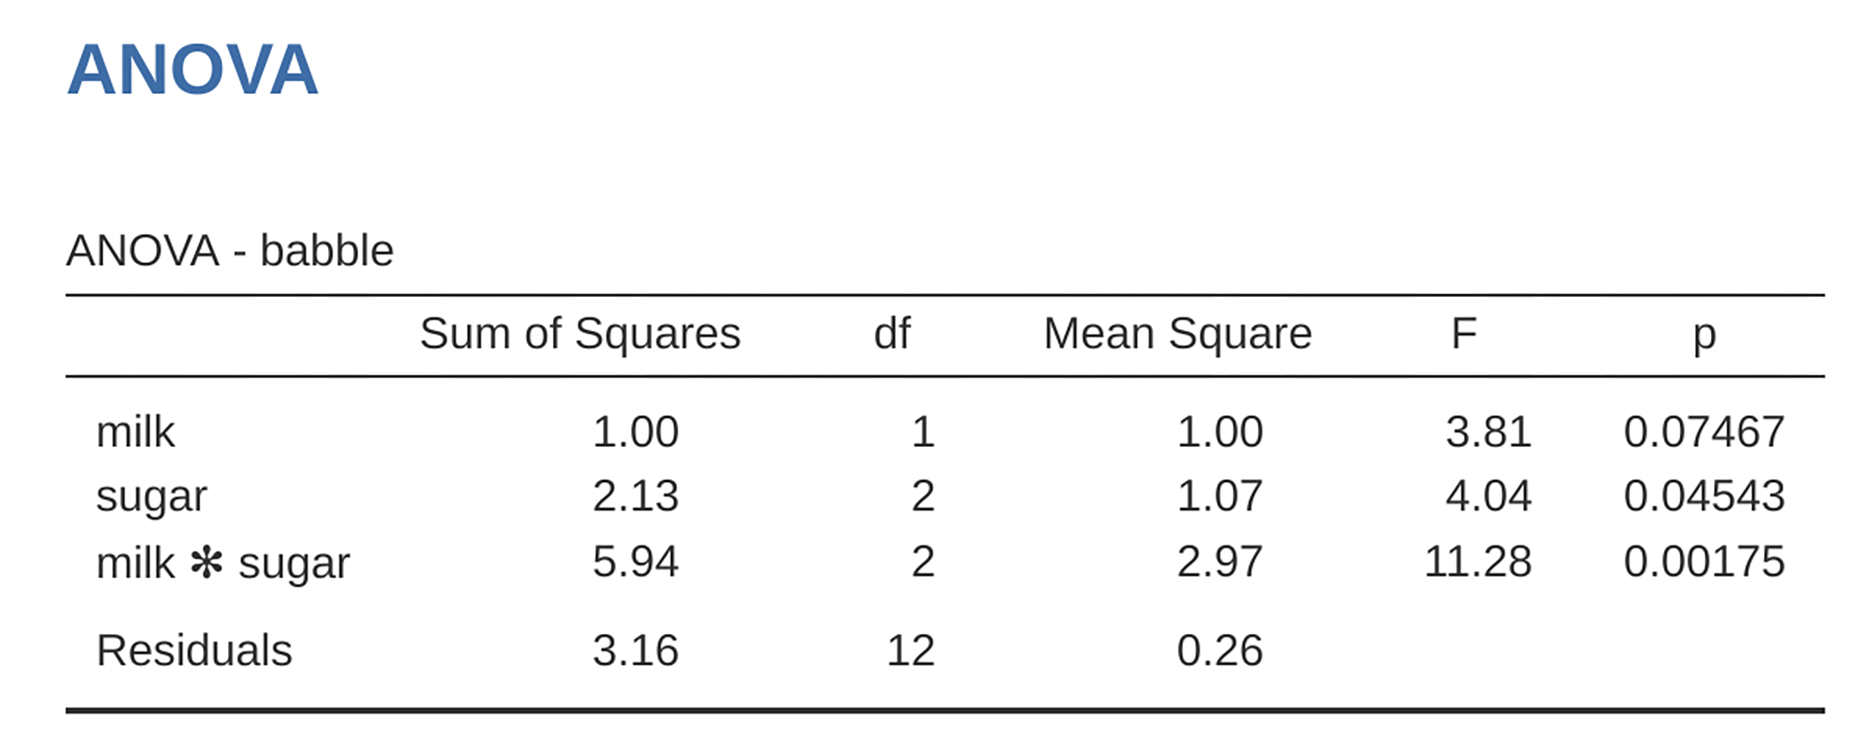
\includegraphics[width=1\textwidth,height=\textheight]{images/fig14-29.png} \hfill{}

\caption{\label{fig-fig14-29}ANOVA results table using type III sum of
squares in jamovi}

\end{figure}

But be aware, one of the perverse features of the type III testing
strategy is that typically the results turn out to depend on the
contrasts that you use to encode your factors (see the
\protect\hyperlink{different-ways-to-specify-contrasts}{Different ways
to specify contrasts} section if you've forgotten what the different
types of contrasts are).\footnote{However, in jamovi the results for
  type III sum of squares ANOVA are the same regardless of the contrast
  selected, so jamovi is obviously doing something different!}

Okay, so if the \(p\)-values that typically come out of type III
analyses (but not in jamovi) are so sensitive to the choice of
contrasts, does that mean that type III tests are essentially arbitrary
and not to be trusted? To some extent that's true, and when we turn to a
discussion of type II tests we'll see that type II analyses avoid this
arbitrariness entirely, but I think that's too strong a conclusion.
Firstly, it's important to recognise that some choices of contrasts will
always produce the same answers (ah, so this is what is happening in
jamovi). Of particular importance is the fact that if the columns of our
contrast matrix are all constrained to sum to zero, then the type III
analysis will always give the same answers.

\hypertarget{type-ii-sum-of-squares}{%
\subsection{Type II sum of squares}\label{type-ii-sum-of-squares}}

Okay, so we've seen type I and III tests now, and both are pretty
straightforward. Type I tests are performed by gradually adding terms
one at a time, whereas type III tests are performed by taking the full
model and looking to see what happens when you remove each term.
However, both can have some limitations. Type I tests are dependent on
the order in which you enter the terms, and type III tests are dependent
on how you code up your contrasts. Type II tests are a little harder to
describe, but they avoid both of these problems, and as a result they
are a little easier to interpret.

Type II tests are broadly similar to type III tests. Start with a
``full'' model, and test a particular term by deleting it from that
model. However, type II tests are based on the marginality principle
which states that you should not omit a lower order term from your model
if there are any higher order ones that depend on it. So, for instance,
if your model contains the two-way interaction A \(\times\) B (a 2nd
order term), then it really ought to contain the main effects A and B
(1st order terms). Similarly, if it contains a three-way interaction
term A \(\times\) B \(\times\) C, then the model must also include the
main effects A, B and C as well as the simpler interactions A \(\times\)
B, A \(\times\) C and B \(\times\) C. Type III tests routinely violate
the marginality principle. For instance, consider the test of the main
effect of A in the context of a three-way ANOVA that includes all
possible interaction terms. According to type III tests, our null and
alternative models are in Table~\ref{tbl-tab14-23}.

\hypertarget{tbl-tab14-23}{}
 
  \providecommand{\huxb}[2]{\arrayrulecolor[RGB]{#1}\global\arrayrulewidth=#2pt}
  \providecommand{\huxvb}[2]{\color[RGB]{#1}\vrule width #2pt}
  \providecommand{\huxtpad}[1]{\rule{0pt}{#1}}
  \providecommand{\huxbpad}[1]{\rule[-#1]{0pt}{#1}}

\begin{table}[ht]
\caption{\label{tbl-tab14-23}Type III tests for a main effect, A, in a three-way ANOVA with all
possible interaction terms }\tabularnewline

\begin{centerbox}
\begin{threeparttable}
\setlength{\tabcolsep}{0pt}
\begin{tabularx}{0.9\textwidth}{p{0.45\textwidth} p{0.45\textwidth}}


\hhline{>{\huxb{0, 0, 0}{0.4}}->{\huxb{0, 0, 0}{0.4}}-}
\arrayrulecolor{black}

\multicolumn{1}{!{\huxvb{0, 0, 0}{0}}p{0.45\textwidth}!{\huxvb{0, 0, 0}{0}}}{\hspace{0pt}\parbox[b]{0.45\textwidth-0pt-12pt}{\huxtpad{2pt + 1em}\centering \textbf{Null model:}\huxbpad{2pt}}} &
\multicolumn{1}{p{0.45\textwidth}!{\huxvb{0, 0, 0}{0}}}{\hspace{12pt}\parbox[b]{0.45\textwidth-12pt-0pt}{\huxtpad{2pt + 1em}\centering \textbf{\(outcome \sim B + C + A*B + A*C + B*C + A*B*C\)}\huxbpad{2pt}}} \tabularnewline[-0.5pt]


\hhline{>{\huxb{0, 0, 0}{0.4}}->{\huxb{0, 0, 0}{0.4}}-}
\arrayrulecolor{black}

\multicolumn{1}{!{\huxvb{0, 0, 0}{0}}p{0.45\textwidth}!{\huxvb{0, 0, 0}{0}}}{\hspace{0pt}\parbox[b]{0.45\textwidth-0pt-12pt}{\huxtpad{2pt + 1em}\centering Alternative model:\huxbpad{2pt}}} &
\multicolumn{1}{p{0.45\textwidth}!{\huxvb{0, 0, 0}{0}}}{\hspace{12pt}\parbox[b]{0.45\textwidth-12pt-0pt}{\huxtpad{2pt + 1em}\centering \(outcome \sim A + B + C + A*B + A*C + B*C + A*B*C\)\huxbpad{2pt}}} \tabularnewline[-0.5pt]


\hhline{>{\huxb{0, 0, 0}{0.4}}->{\huxb{0, 0, 0}{0.4}}-}
\arrayrulecolor{black}
\end{tabularx} 

\end{threeparttable}\par\end{centerbox}

\end{table}
 

Notice that the null hypothesis omits A, but includes A \(\times\) B, A
\(\times\) C and A \(\times\) B \(\times\) C as part of the model. This,
according to the type II tests, is not a good choice of null hypothesis.
What we should do instead, if we want to test the null hypothesis that A
is not relevant to our outcome, is to specify the null hypothesis that
is the most complicated model that does not rely on A in any form, even
as an interaction. The alternative hypothesis corresponds to this null
model plus a main effect term of A. This is a lot closer to what most
people would intuitively think of as a ``main effect of A'', and it
yields the following as our Type II test of the main effect of A
(Table~\ref{tbl-tab14-24}).\footnote{Note, of course, that this does
  depend on the model that the user specified. If the original ANOVA
  model doesn't contain an interaction term for \(B \times C\), then
  obviously it won't appear in either the null or the alternative. But
  that's true for types I, II and III. They never include any terms that
  you didn't include, but they make different choices about how to
  construct tests for the ones that you did include.}

\hypertarget{tbl-tab14-24}{}
 
  \providecommand{\huxb}[2]{\arrayrulecolor[RGB]{#1}\global\arrayrulewidth=#2pt}
  \providecommand{\huxvb}[2]{\color[RGB]{#1}\vrule width #2pt}
  \providecommand{\huxtpad}[1]{\rule{0pt}{#1}}
  \providecommand{\huxbpad}[1]{\rule[-#1]{0pt}{#1}}

\begin{table}[ht]
\caption{\label{tbl-tab14-24}Type II tests for a main effect, A, in a three-way ANOVA with all
possible interaction terms }\tabularnewline

\begin{centerbox}
\begin{threeparttable}
\setlength{\tabcolsep}{0pt}
\begin{tabularx}{0.9\textwidth}{p{0.45\textwidth} p{0.45\textwidth}}


\hhline{>{\huxb{0, 0, 0}{0.4}}->{\huxb{0, 0, 0}{0.4}}-}
\arrayrulecolor{black}

\multicolumn{1}{!{\huxvb{0, 0, 0}{0}}p{0.45\textwidth}!{\huxvb{0, 0, 0}{0}}}{\hspace{0pt}\parbox[b]{0.45\textwidth-0pt-12pt}{\huxtpad{2pt + 1em}\centering \textbf{Null model:}\huxbpad{2pt}}} &
\multicolumn{1}{p{0.45\textwidth}!{\huxvb{0, 0, 0}{0}}}{\hspace{12pt}\parbox[b]{0.45\textwidth-12pt-0pt}{\huxtpad{2pt + 1em}\centering \textbf{\(outcome \sim B + C + B*C\)}\huxbpad{2pt}}} \tabularnewline[-0.5pt]


\hhline{>{\huxb{0, 0, 0}{0.4}}->{\huxb{0, 0, 0}{0.4}}-}
\arrayrulecolor{black}

\multicolumn{1}{!{\huxvb{0, 0, 0}{0}}p{0.45\textwidth}!{\huxvb{0, 0, 0}{0}}}{\hspace{0pt}\parbox[b]{0.45\textwidth-0pt-12pt}{\huxtpad{2pt + 1em}\centering Alternative model:\huxbpad{2pt}}} &
\multicolumn{1}{p{0.45\textwidth}!{\huxvb{0, 0, 0}{0}}}{\hspace{12pt}\parbox[b]{0.45\textwidth-12pt-0pt}{\huxtpad{2pt + 1em}\centering \(outcome \sim A + B + C + B*C\)\huxbpad{2pt}}} \tabularnewline[-0.5pt]


\hhline{>{\huxb{0, 0, 0}{0.4}}->{\huxb{0, 0, 0}{0.4}}-}
\arrayrulecolor{black}
\end{tabularx} 

\end{threeparttable}\par\end{centerbox}

\end{table}
 

Anyway, just to give you a sense of how the type II tests play out, see
the full table (Table~\ref{tbl-tab14-25}) of tests that would be applied
in a three-way factorial ANOVA.

\hypertarget{tbl-tab14-25}{}
 
  \providecommand{\huxb}[2]{\arrayrulecolor[RGB]{#1}\global\arrayrulewidth=#2pt}
  \providecommand{\huxvb}[2]{\color[RGB]{#1}\vrule width #2pt}
  \providecommand{\huxtpad}[1]{\rule{0pt}{#1}}
  \providecommand{\huxbpad}[1]{\rule[-#1]{0pt}{#1}}

\begin{table}[ht]
\caption{\label{tbl-tab14-25}Type II tests for a three-way factorial model }\tabularnewline

\begin{centerbox}
\begin{threeparttable}
\setlength{\tabcolsep}{0pt}
\begin{tabularx}{0.9\textwidth}{p{0.3\textwidth} p{0.3\textwidth} p{0.3\textwidth}}


\hhline{>{\huxb{0, 0, 0}{0.4}}->{\huxb{0, 0, 0}{0.4}}->{\huxb{0, 0, 0}{0.4}}-}
\arrayrulecolor{black}

\multicolumn{1}{!{\huxvb{0, 0, 0}{0}}p{0.3\textwidth}!{\huxvb{0, 0, 0}{0}}}{\hspace{0pt}\parbox[b]{0.3\textwidth-0pt-12pt}{\huxtpad{2pt + 1em}\centering \textbf{Term being tested is}\huxbpad{2pt}}} &
\multicolumn{1}{p{0.3\textwidth}!{\huxvb{0, 0, 0}{0}}}{\hspace{12pt}\parbox[b]{0.3\textwidth-12pt-12pt}{\huxtpad{2pt + 1em}\centering \textbf{Null model is outcome ~ ...}\huxbpad{2pt}}} &
\multicolumn{1}{p{0.3\textwidth}!{\huxvb{0, 0, 0}{0}}}{\hspace{12pt}\parbox[b]{0.3\textwidth-12pt-0pt}{\huxtpad{2pt + 1em}\centering \textbf{Alternative model is outcome ~ ...}\huxbpad{2pt}}} \tabularnewline[-0.5pt]


\hhline{>{\huxb{0, 0, 0}{0.4}}->{\huxb{0, 0, 0}{0.4}}->{\huxb{0, 0, 0}{0.4}}-}
\arrayrulecolor{black}

\multicolumn{1}{!{\huxvb{0, 0, 0}{0}}p{0.3\textwidth}!{\huxvb{0, 0, 0}{0}}}{\hspace{0pt}\parbox[b]{0.3\textwidth-0pt-12pt}{\huxtpad{2pt + 1em}\centering A\huxbpad{2pt}}} &
\multicolumn{1}{p{0.3\textwidth}!{\huxvb{0, 0, 0}{0}}}{\hspace{12pt}\parbox[b]{0.3\textwidth-12pt-12pt}{\huxtpad{2pt + 1em}\centering \(B + C + B*C \)\huxbpad{2pt}}} &
\multicolumn{1}{p{0.3\textwidth}!{\huxvb{0, 0, 0}{0}}}{\hspace{12pt}\parbox[b]{0.3\textwidth-12pt-0pt}{\huxtpad{2pt + 1em}\centering \(A + B + C + B*C \)\huxbpad{2pt}}} \tabularnewline[-0.5pt]


\hhline{}
\arrayrulecolor{black}

\multicolumn{1}{!{\huxvb{0, 0, 0}{0}}p{0.3\textwidth}!{\huxvb{0, 0, 0}{0}}}{\hspace{0pt}\parbox[b]{0.3\textwidth-0pt-12pt}{\huxtpad{2pt + 1em}\centering B\huxbpad{2pt}}} &
\multicolumn{1}{p{0.3\textwidth}!{\huxvb{0, 0, 0}{0}}}{\hspace{12pt}\parbox[b]{0.3\textwidth-12pt-12pt}{\huxtpad{2pt + 1em}\centering \(A + C + A*C \)\huxbpad{2pt}}} &
\multicolumn{1}{p{0.3\textwidth}!{\huxvb{0, 0, 0}{0}}}{\hspace{12pt}\parbox[b]{0.3\textwidth-12pt-0pt}{\huxtpad{2pt + 1em}\centering \(A + B + C + A*C\)\huxbpad{2pt}}} \tabularnewline[-0.5pt]


\hhline{}
\arrayrulecolor{black}

\multicolumn{1}{!{\huxvb{0, 0, 0}{0}}p{0.3\textwidth}!{\huxvb{0, 0, 0}{0}}}{\hspace{0pt}\parbox[b]{0.3\textwidth-0pt-12pt}{\huxtpad{2pt + 1em}\centering C\huxbpad{2pt}}} &
\multicolumn{1}{p{0.3\textwidth}!{\huxvb{0, 0, 0}{0}}}{\hspace{12pt}\parbox[b]{0.3\textwidth-12pt-12pt}{\huxtpad{2pt + 1em}\centering \(A + B + A*B \)\huxbpad{2pt}}} &
\multicolumn{1}{p{0.3\textwidth}!{\huxvb{0, 0, 0}{0}}}{\hspace{12pt}\parbox[b]{0.3\textwidth-12pt-0pt}{\huxtpad{2pt + 1em}\centering \(A + B + C + A*B\)\huxbpad{2pt}}} \tabularnewline[-0.5pt]


\hhline{}
\arrayrulecolor{black}

\multicolumn{1}{!{\huxvb{0, 0, 0}{0}}p{0.3\textwidth}!{\huxvb{0, 0, 0}{0}}}{\hspace{0pt}\parbox[b]{0.3\textwidth-0pt-12pt}{\huxtpad{2pt + 1em}\centering A*B\huxbpad{2pt}}} &
\multicolumn{1}{p{0.3\textwidth}!{\huxvb{0, 0, 0}{0}}}{\hspace{12pt}\parbox[b]{0.3\textwidth-12pt-12pt}{\huxtpad{2pt + 1em}\centering \(A + B + C + A*C + B*C  \)\huxbpad{2pt}}} &
\multicolumn{1}{p{0.3\textwidth}!{\huxvb{0, 0, 0}{0}}}{\hspace{12pt}\parbox[b]{0.3\textwidth-12pt-0pt}{\huxtpad{2pt + 1em}\centering \(A + B + C + A*B + A*C + B*C \)\huxbpad{2pt}}} \tabularnewline[-0.5pt]


\hhline{}
\arrayrulecolor{black}

\multicolumn{1}{!{\huxvb{0, 0, 0}{0}}p{0.3\textwidth}!{\huxvb{0, 0, 0}{0}}}{\hspace{0pt}\parbox[b]{0.3\textwidth-0pt-12pt}{\huxtpad{2pt + 1em}\centering A*C\huxbpad{2pt}}} &
\multicolumn{1}{p{0.3\textwidth}!{\huxvb{0, 0, 0}{0}}}{\hspace{12pt}\parbox[b]{0.3\textwidth-12pt-12pt}{\huxtpad{2pt + 1em}\centering \(A + B + C + A*B + B*C  \)\huxbpad{2pt}}} &
\multicolumn{1}{p{0.3\textwidth}!{\huxvb{0, 0, 0}{0}}}{\hspace{12pt}\parbox[b]{0.3\textwidth-12pt-0pt}{\huxtpad{2pt + 1em}\centering \(A + B + C + A*B + A*C + B*C \)\huxbpad{2pt}}} \tabularnewline[-0.5pt]


\hhline{}
\arrayrulecolor{black}

\multicolumn{1}{!{\huxvb{0, 0, 0}{0}}p{0.3\textwidth}!{\huxvb{0, 0, 0}{0}}}{\hspace{0pt}\parbox[b]{0.3\textwidth-0pt-12pt}{\huxtpad{2pt + 1em}\centering B*C\huxbpad{2pt}}} &
\multicolumn{1}{p{0.3\textwidth}!{\huxvb{0, 0, 0}{0}}}{\hspace{12pt}\parbox[b]{0.3\textwidth-12pt-12pt}{\huxtpad{2pt + 1em}\centering \(A + B + C + A*B + A*C \)\huxbpad{2pt}}} &
\multicolumn{1}{p{0.3\textwidth}!{\huxvb{0, 0, 0}{0}}}{\hspace{12pt}\parbox[b]{0.3\textwidth-12pt-0pt}{\huxtpad{2pt + 1em}\centering \(A + B + C + A*B + A*C + B*C \)\huxbpad{2pt}}} \tabularnewline[-0.5pt]


\hhline{}
\arrayrulecolor{black}

\multicolumn{1}{!{\huxvb{0, 0, 0}{0}}p{0.3\textwidth}!{\huxvb{0, 0, 0}{0}}}{\hspace{0pt}\parbox[b]{0.3\textwidth-0pt-12pt}{\huxtpad{2pt + 1em}\centering A*B*C\huxbpad{2pt}}} &
\multicolumn{1}{p{0.3\textwidth}!{\huxvb{0, 0, 0}{0}}}{\hspace{12pt}\parbox[b]{0.3\textwidth-12pt-12pt}{\huxtpad{2pt + 1em}\centering \(A + B + C + A*B + A*C + B*C \)\huxbpad{2pt}}} &
\multicolumn{1}{p{0.3\textwidth}!{\huxvb{0, 0, 0}{0}}}{\hspace{12pt}\parbox[b]{0.3\textwidth-12pt-0pt}{\huxtpad{2pt + 1em}\centering \(A + B + C + A*B + A*C + B*C + A*B*C \)\huxbpad{2pt}}} \tabularnewline[-0.5pt]


\hhline{>{\huxb{0, 0, 0}{0.4}}->{\huxb{0, 0, 0}{0.4}}->{\huxb{0, 0, 0}{0.4}}-}
\arrayrulecolor{black}
\end{tabularx} 

\end{threeparttable}\par\end{centerbox}

\end{table}
 

In the context of the two way ANOVA that we've been using in the
\emph{coffee} data, the hypothesis tests are even simpler. The main
effect of sugar corresponds to an \(F\)-test comparing these two models
(Table~\ref{tbl-tab14-26}).

\hypertarget{tbl-tab14-26}{}
 
  \providecommand{\huxb}[2]{\arrayrulecolor[RGB]{#1}\global\arrayrulewidth=#2pt}
  \providecommand{\huxvb}[2]{\color[RGB]{#1}\vrule width #2pt}
  \providecommand{\huxtpad}[1]{\rule{0pt}{#1}}
  \providecommand{\huxbpad}[1]{\rule[-#1]{0pt}{#1}}

\begin{table}[ht]
\caption{\label{tbl-tab14-26}Type II tests for the main effect of sugar in the \emph{coffee} data }\tabularnewline

\begin{centerbox}
\begin{threeparttable}
\setlength{\tabcolsep}{0pt}
\begin{tabularx}{0.9\textwidth}{p{0.45\textwidth} p{0.45\textwidth}}


\hhline{>{\huxb{0, 0, 0}{0.4}}->{\huxb{0, 0, 0}{0.4}}-}
\arrayrulecolor{black}

\multicolumn{1}{!{\huxvb{0, 0, 0}{0}}p{0.45\textwidth}!{\huxvb{0, 0, 0}{0}}}{\hspace{0pt}\parbox[b]{0.45\textwidth-0pt-12pt}{\huxtpad{2pt + 1em}\centering \textbf{Null model:}\huxbpad{2pt}}} &
\multicolumn{1}{p{0.45\textwidth}!{\huxvb{0, 0, 0}{0}}}{\hspace{12pt}\parbox[b]{0.45\textwidth-12pt-0pt}{\huxtpad{2pt + 1em}\centering \textbf{\(babble \sim milk \)}\huxbpad{2pt}}} \tabularnewline[-0.5pt]


\hhline{>{\huxb{0, 0, 0}{0.4}}->{\huxb{0, 0, 0}{0.4}}-}
\arrayrulecolor{black}

\multicolumn{1}{!{\huxvb{0, 0, 0}{0}}p{0.45\textwidth}!{\huxvb{0, 0, 0}{0}}}{\hspace{0pt}\parbox[b]{0.45\textwidth-0pt-12pt}{\huxtpad{2pt + 1em}\centering Alternative model:\huxbpad{2pt}}} &
\multicolumn{1}{p{0.45\textwidth}!{\huxvb{0, 0, 0}{0}}}{\hspace{12pt}\parbox[b]{0.45\textwidth-12pt-0pt}{\huxtpad{2pt + 1em}\centering \(babble \sim sugar + milk\)\huxbpad{2pt}}} \tabularnewline[-0.5pt]


\hhline{>{\huxb{0, 0, 0}{0.4}}->{\huxb{0, 0, 0}{0.4}}-}
\arrayrulecolor{black}
\end{tabularx} 

\end{threeparttable}\par\end{centerbox}

\end{table}
 

The test for the main effect of milk is in Table~\ref{tbl-tab14-27}.

\hypertarget{tbl-tab14-27}{}
 
  \providecommand{\huxb}[2]{\arrayrulecolor[RGB]{#1}\global\arrayrulewidth=#2pt}
  \providecommand{\huxvb}[2]{\color[RGB]{#1}\vrule width #2pt}
  \providecommand{\huxtpad}[1]{\rule{0pt}{#1}}
  \providecommand{\huxbpad}[1]{\rule[-#1]{0pt}{#1}}

\begin{table}[ht]
\caption{\label{tbl-tab14-27}Type II tests for the main effect of milk in the \emph{coffee} data }\tabularnewline

\begin{centerbox}
\begin{threeparttable}
\setlength{\tabcolsep}{0pt}
\begin{tabularx}{0.9\textwidth}{p{0.45\textwidth} p{0.45\textwidth}}


\hhline{>{\huxb{0, 0, 0}{0.4}}->{\huxb{0, 0, 0}{0.4}}-}
\arrayrulecolor{black}

\multicolumn{1}{!{\huxvb{0, 0, 0}{0}}p{0.45\textwidth}!{\huxvb{0, 0, 0}{0}}}{\hspace{0pt}\parbox[b]{0.45\textwidth-0pt-12pt}{\huxtpad{2pt + 1em}\centering \textbf{Null model:}\huxbpad{2pt}}} &
\multicolumn{1}{p{0.45\textwidth}!{\huxvb{0, 0, 0}{0}}}{\hspace{12pt}\parbox[b]{0.45\textwidth-12pt-0pt}{\huxtpad{2pt + 1em}\centering \textbf{\(babble \sim  sugar \)}\huxbpad{2pt}}} \tabularnewline[-0.5pt]


\hhline{>{\huxb{0, 0, 0}{0.4}}->{\huxb{0, 0, 0}{0.4}}-}
\arrayrulecolor{black}

\multicolumn{1}{!{\huxvb{0, 0, 0}{0}}p{0.45\textwidth}!{\huxvb{0, 0, 0}{0}}}{\hspace{0pt}\parbox[b]{0.45\textwidth-0pt-12pt}{\huxtpad{2pt + 1em}\centering Alternative model:\huxbpad{2pt}}} &
\multicolumn{1}{p{0.45\textwidth}!{\huxvb{0, 0, 0}{0}}}{\hspace{12pt}\parbox[b]{0.45\textwidth-12pt-0pt}{\huxtpad{2pt + 1em}\centering \(babble \sim sugar + milk\)\huxbpad{2pt}}} \tabularnewline[-0.5pt]


\hhline{>{\huxb{0, 0, 0}{0.4}}->{\huxb{0, 0, 0}{0.4}}-}
\arrayrulecolor{black}
\end{tabularx} 

\end{threeparttable}\par\end{centerbox}

\end{table}
 

Finally, the test for the interaction sugar \(\times\) milk is in
Table~\ref{tbl-tab14-28}.

\hypertarget{tbl-tab14-28}{}
 
  \providecommand{\huxb}[2]{\arrayrulecolor[RGB]{#1}\global\arrayrulewidth=#2pt}
  \providecommand{\huxvb}[2]{\color[RGB]{#1}\vrule width #2pt}
  \providecommand{\huxtpad}[1]{\rule{0pt}{#1}}
  \providecommand{\huxbpad}[1]{\rule[-#1]{0pt}{#1}}

\begin{table}[ht]
\caption{\label{tbl-tab14-28}Type II tests for the sugar \(\times\) milk interaction term }\tabularnewline

\begin{centerbox}
\begin{threeparttable}
\setlength{\tabcolsep}{0pt}
\begin{tabularx}{0.9\textwidth}{p{0.45\textwidth} p{0.45\textwidth}}


\hhline{>{\huxb{0, 0, 0}{0.4}}->{\huxb{0, 0, 0}{0.4}}-}
\arrayrulecolor{black}

\multicolumn{1}{!{\huxvb{0, 0, 0}{0}}p{0.45\textwidth}!{\huxvb{0, 0, 0}{0}}}{\hspace{0pt}\parbox[b]{0.45\textwidth-0pt-12pt}{\huxtpad{2pt + 1em}\centering \textbf{Null model:}\huxbpad{2pt}}} &
\multicolumn{1}{p{0.45\textwidth}!{\huxvb{0, 0, 0}{0}}}{\hspace{12pt}\parbox[b]{0.45\textwidth-12pt-0pt}{\huxtpad{2pt + 1em}\centering \textbf{\(babble \sim  sugar + milk \)}\huxbpad{2pt}}} \tabularnewline[-0.5pt]


\hhline{>{\huxb{0, 0, 0}{0.4}}->{\huxb{0, 0, 0}{0.4}}-}
\arrayrulecolor{black}

\multicolumn{1}{!{\huxvb{0, 0, 0}{0}}p{0.45\textwidth}!{\huxvb{0, 0, 0}{0}}}{\hspace{0pt}\parbox[b]{0.45\textwidth-0pt-12pt}{\huxtpad{2pt + 1em}\centering Alternative model:\huxbpad{2pt}}} &
\multicolumn{1}{p{0.45\textwidth}!{\huxvb{0, 0, 0}{0}}}{\hspace{12pt}\parbox[b]{0.45\textwidth-12pt-0pt}{\huxtpad{2pt + 1em}\centering \(babble \sim sugar + milk  + sugar*milk \)\huxbpad{2pt}}} \tabularnewline[-0.5pt]


\hhline{>{\huxb{0, 0, 0}{0.4}}->{\huxb{0, 0, 0}{0.4}}-}
\arrayrulecolor{black}
\end{tabularx} 

\end{threeparttable}\par\end{centerbox}

\end{table}
 

Running the tests are again straightforward. Just select `Type 2' in the
`Sum of squares' selection box in the jamovi `ANOVA' - `Model' options,
This gives us the ANOVA table shown in Figure~\ref{fig-fig14-30}.

\begin{figure}

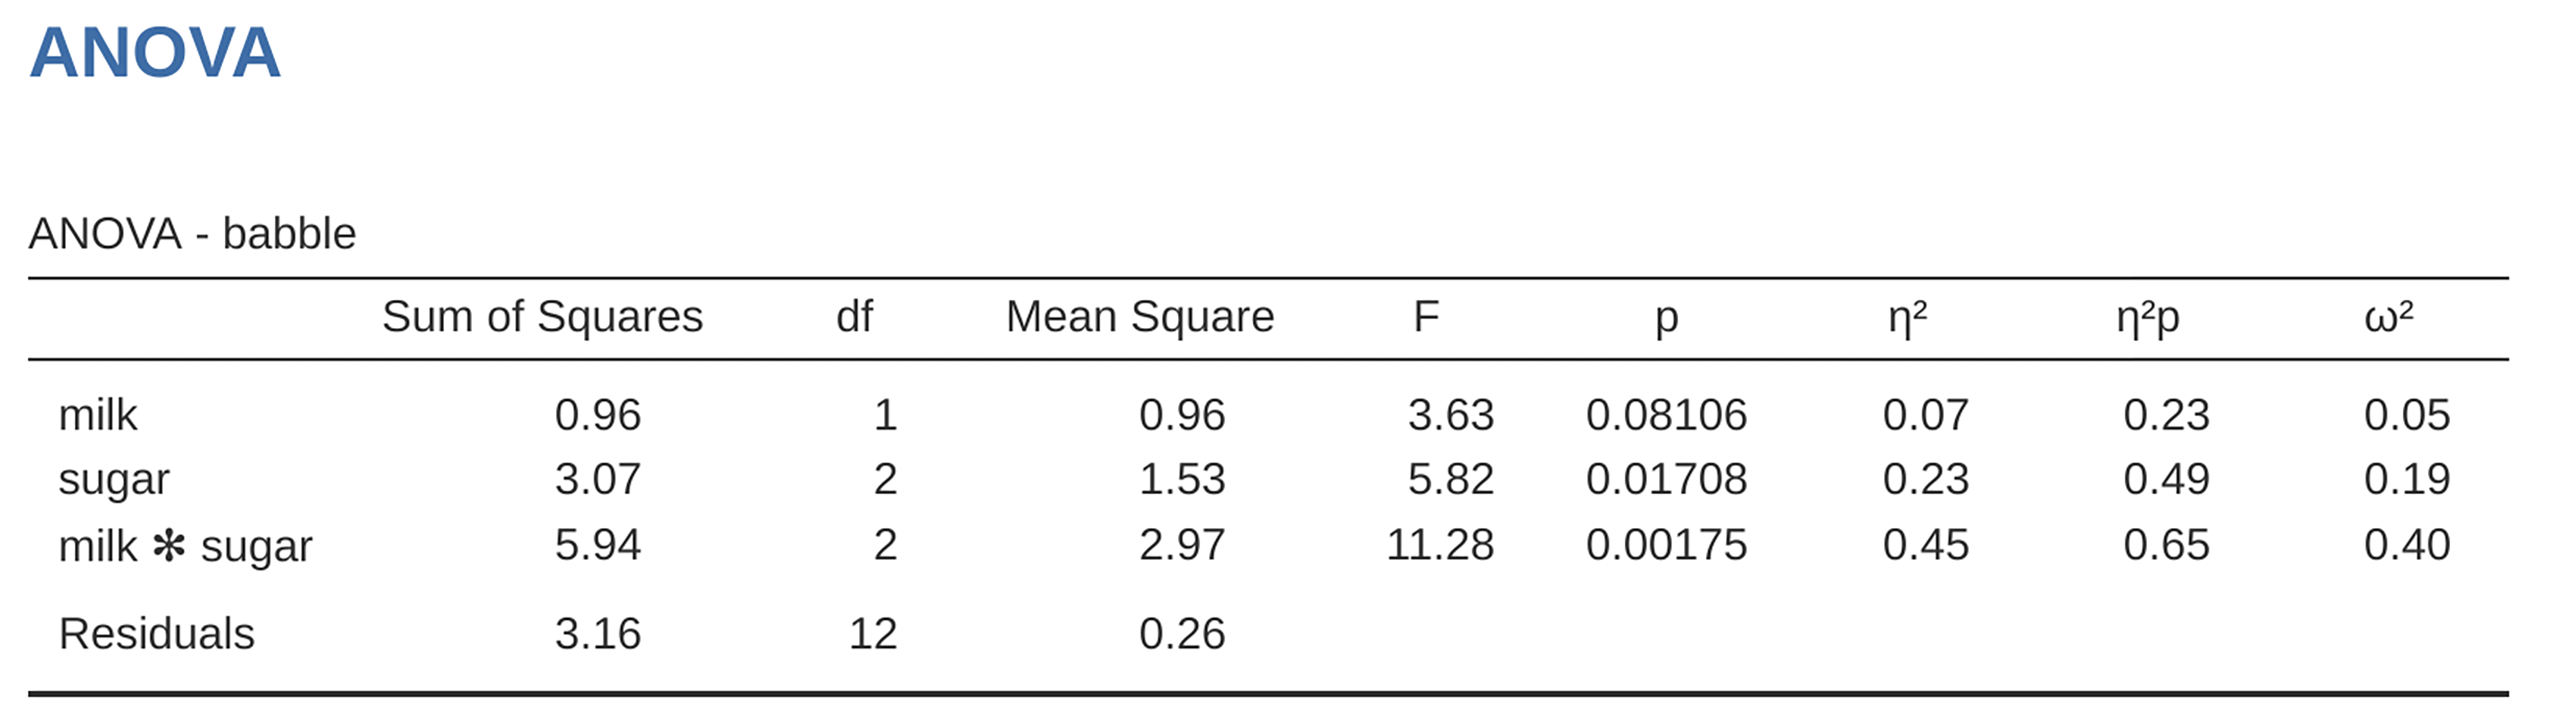
\includegraphics[width=1\textwidth,height=\textheight]{images/fig14-30.png} \hfill{}

\caption{\label{fig-fig14-30}ANOVA results table using type II sum of
squares in jamovi}

\end{figure}

Type II tests have some clear advantages over type I and type III tests.
They don't depend on the order in which you specify factors (unlike type
I), and they don't depend on the contrasts that you use to specify your
factors (unlike type III). And although opinions may differ on this last
point, and it will definitely depend on what you're trying to do with
your data, I do think that the hypothesis tests that they specify are
more likely to correspond to something that you actually care about. As
a consequence, I find that it's usually easier to interpret the results
of a type II test than the results of a type I or type III test. For
this reason my tentative advice is that, if you can't think of any
obvious model comparisons that directly map onto your research questions
but you still want to run an ANOVA in an unbalanced design, type II
tests are probably a better choice than type I or type III.\footnote{I
  find it amusing to note that the default in \(R\) is type I and the
  default in SPSS and jamovi is type III. Neither of these appeals to me
  all that much. Relatedly, I find it depressing that almost nobody in
  the psychological literature ever bothers to report which type is used
  either. The only way I can ever make any sense of what people
  typically report is to try to guess from auxiliary cues which software
  they were using, and to assume that they never changed the default
  settings. Please don't do this! Now that you know about these issues
  make sure you indicate what software you used, and if you're reporting
  ANOVA results for unbalanced data, then specify what Type of tests you
  ran, specify order information if you've done type I tests and specify
  contrasts if you've done type III tests. Or, even better, do
  hypotheses tests that correspond to things you really care about and
  then report those!}

\hypertarget{effect-sizes-and-non-additive-sums-of-squares}{%
\subsection{Effect sizes (and non-additive sums of
squares)}\label{effect-sizes-and-non-additive-sums-of-squares}}

jamovi also provides the effect sizes \(\eta^2\) and partial \(\eta^2\)
when you select these options, as in Figure~\ref{fig-fig14-30}. However,
when you've got an unbalanced design there's a bit of extra complexity
involved.

If you remember back to our very early discussions of ANOVA, one of the
key ideas behind the sums of squares calculations is that if we add up
all the \(SS\) terms associated with the effects in the model, and add
that to the residual \(SS\), they're supposed to add up to the total sum
of squares. And, on top of that, the whole idea behind \(\eta^2\) is
that, because you're dividing one of the \(SS\) terms by the total
\(SS\) value, an \(\eta^2\) value can be interpreted as the proportion
of variance accounted for by a particular term. But this is not so
straightforward in unbalanced designs because some of the variance goes
``missing''.

This seems a bit odd at first, but here's why. When you have unbalanced
designs your factors become correlated with one another, and it becomes
difficult to tell the difference between the effect of Factor A and the
effect of Factor B. In the extreme case, suppose that we'd run a
\(2 \times 2\) design in which the number of participants in each group
had been as in Table~\ref{tbl-tab14-29}.

\hypertarget{tbl-tab14-29}{}
 
  \providecommand{\huxb}[2]{\arrayrulecolor[RGB]{#1}\global\arrayrulewidth=#2pt}
  \providecommand{\huxvb}[2]{\color[RGB]{#1}\vrule width #2pt}
  \providecommand{\huxtpad}[1]{\rule{0pt}{#1}}
  \providecommand{\huxbpad}[1]{\rule[-#1]{0pt}{#1}}

\begin{table}[ht]
\caption{\label{tbl-tab14-29}\(N\) participants in a 2 x 2 very (very!) unbalanced factorial design }\tabularnewline

\begin{centerbox}
\begin{threeparttable}
\setlength{\tabcolsep}{0pt}
\begin{tabularx}{0.9\textwidth}{p{0.3\textwidth} p{0.3\textwidth} p{0.3\textwidth}}


\hhline{>{\huxb{0, 0, 0}{0.4}}->{\huxb{0, 0, 0}{0.4}}->{\huxb{0, 0, 0}{0.4}}-}
\arrayrulecolor{black}

\multicolumn{1}{!{\huxvb{0, 0, 0}{0}}p{0.3\textwidth}!{\huxvb{0, 0, 0}{0}}}{\hspace{0pt}\parbox[b]{0.3\textwidth-0pt-12pt}{\huxtpad{2pt + 1em}\centering \textbf{}\huxbpad{2pt}}} &
\multicolumn{1}{p{0.3\textwidth}!{\huxvb{0, 0, 0}{0}}}{\hspace{12pt}\parbox[b]{0.3\textwidth-12pt-12pt}{\huxtpad{2pt + 1em}\centering \textbf{sugar}\huxbpad{2pt}}} &
\multicolumn{1}{p{0.3\textwidth}!{\huxvb{0, 0, 0}{0}}}{\hspace{12pt}\parbox[b]{0.3\textwidth-12pt-0pt}{\huxtpad{2pt + 1em}\centering \textbf{no sugar}\huxbpad{2pt}}} \tabularnewline[-0.5pt]


\hhline{>{\huxb{0, 0, 0}{0.4}}->{\huxb{0, 0, 0}{0.4}}->{\huxb{0, 0, 0}{0.4}}-}
\arrayrulecolor{black}

\multicolumn{1}{!{\huxvb{0, 0, 0}{0}}p{0.3\textwidth}!{\huxvb{0, 0, 0}{0}}}{\hspace{0pt}\parbox[b]{0.3\textwidth-0pt-12pt}{\huxtpad{2pt + 1em}\centering milk\huxbpad{2pt}}} &
\multicolumn{1}{p{0.3\textwidth}!{\huxvb{0, 0, 0}{0}}}{\hspace{12pt}\parbox[b]{0.3\textwidth-12pt-12pt}{\huxtpad{2pt + 1em}\centering 100\huxbpad{2pt}}} &
\multicolumn{1}{p{0.3\textwidth}!{\huxvb{0, 0, 0}{0}}}{\hspace{12pt}\parbox[b]{0.3\textwidth-12pt-0pt}{\huxtpad{2pt + 1em}\centering 0\huxbpad{2pt}}} \tabularnewline[-0.5pt]


\hhline{}
\arrayrulecolor{black}

\multicolumn{1}{!{\huxvb{0, 0, 0}{0}}p{0.3\textwidth}!{\huxvb{0, 0, 0}{0}}}{\hspace{0pt}\parbox[b]{0.3\textwidth-0pt-12pt}{\huxtpad{2pt + 1em}\centering no milk\huxbpad{2pt}}} &
\multicolumn{1}{p{0.3\textwidth}!{\huxvb{0, 0, 0}{0}}}{\hspace{12pt}\parbox[b]{0.3\textwidth-12pt-12pt}{\huxtpad{2pt + 1em}\centering 0\huxbpad{2pt}}} &
\multicolumn{1}{p{0.3\textwidth}!{\huxvb{0, 0, 0}{0}}}{\hspace{12pt}\parbox[b]{0.3\textwidth-12pt-0pt}{\huxtpad{2pt + 1em}\centering 100\huxbpad{2pt}}} \tabularnewline[-0.5pt]


\hhline{>{\huxb{0, 0, 0}{0.4}}->{\huxb{0, 0, 0}{0.4}}->{\huxb{0, 0, 0}{0.4}}-}
\arrayrulecolor{black}
\end{tabularx} 

\end{threeparttable}\par\end{centerbox}

\end{table}
 

Here we have a spectacularly unbalanced design: 100 people have milk and
sugar, 100 people have no milk and no sugar, and that's all. There are 0
people with milk and no sugar, and 0 people with sugar but no milk. Now
suppose that, when we collected the data, it turned out there is a large
(and statistically significant) difference between the ``milk and
sugar'' group and the ``no-milk and no-sugar'' group. Is this a main
effect of sugar? A main effect of milk? Or an interaction? It's
impossible to tell, because the presence of sugar has a perfect
association with the presence of milk. Now suppose the design had been a
little more balanced (Table~\ref{tbl-tab14-30}).

\hypertarget{tbl-tab14-30}{}
 
  \providecommand{\huxb}[2]{\arrayrulecolor[RGB]{#1}\global\arrayrulewidth=#2pt}
  \providecommand{\huxvb}[2]{\color[RGB]{#1}\vrule width #2pt}
  \providecommand{\huxtpad}[1]{\rule{0pt}{#1}}
  \providecommand{\huxbpad}[1]{\rule[-#1]{0pt}{#1}}

\begin{table}[ht]
\caption{\label{tbl-tab14-30}\(N\) participants in a 2 x 2 still very unbalanced factorial design }\tabularnewline

\begin{centerbox}
\begin{threeparttable}
\setlength{\tabcolsep}{0pt}
\begin{tabularx}{0.9\textwidth}{p{0.3\textwidth} p{0.3\textwidth} p{0.3\textwidth}}


\hhline{>{\huxb{0, 0, 0}{0.4}}->{\huxb{0, 0, 0}{0.4}}->{\huxb{0, 0, 0}{0.4}}-}
\arrayrulecolor{black}

\multicolumn{1}{!{\huxvb{0, 0, 0}{0}}p{0.3\textwidth}!{\huxvb{0, 0, 0}{0}}}{\hspace{0pt}\parbox[b]{0.3\textwidth-0pt-12pt}{\huxtpad{2pt + 1em}\centering \textbf{}\huxbpad{2pt}}} &
\multicolumn{1}{p{0.3\textwidth}!{\huxvb{0, 0, 0}{0}}}{\hspace{12pt}\parbox[b]{0.3\textwidth-12pt-12pt}{\huxtpad{2pt + 1em}\centering \textbf{sugar}\huxbpad{2pt}}} &
\multicolumn{1}{p{0.3\textwidth}!{\huxvb{0, 0, 0}{0}}}{\hspace{12pt}\parbox[b]{0.3\textwidth-12pt-0pt}{\huxtpad{2pt + 1em}\centering \textbf{no sugar}\huxbpad{2pt}}} \tabularnewline[-0.5pt]


\hhline{>{\huxb{0, 0, 0}{0.4}}->{\huxb{0, 0, 0}{0.4}}->{\huxb{0, 0, 0}{0.4}}-}
\arrayrulecolor{black}

\multicolumn{1}{!{\huxvb{0, 0, 0}{0}}p{0.3\textwidth}!{\huxvb{0, 0, 0}{0}}}{\hspace{0pt}\parbox[b]{0.3\textwidth-0pt-12pt}{\huxtpad{2pt + 1em}\centering milk\huxbpad{2pt}}} &
\multicolumn{1}{p{0.3\textwidth}!{\huxvb{0, 0, 0}{0}}}{\hspace{12pt}\parbox[b]{0.3\textwidth-12pt-12pt}{\huxtpad{2pt + 1em}\centering 100\huxbpad{2pt}}} &
\multicolumn{1}{p{0.3\textwidth}!{\huxvb{0, 0, 0}{0}}}{\hspace{12pt}\parbox[b]{0.3\textwidth-12pt-0pt}{\huxtpad{2pt + 1em}\centering 5\huxbpad{2pt}}} \tabularnewline[-0.5pt]


\hhline{}
\arrayrulecolor{black}

\multicolumn{1}{!{\huxvb{0, 0, 0}{0}}p{0.3\textwidth}!{\huxvb{0, 0, 0}{0}}}{\hspace{0pt}\parbox[b]{0.3\textwidth-0pt-12pt}{\huxtpad{2pt + 1em}\centering no milk\huxbpad{2pt}}} &
\multicolumn{1}{p{0.3\textwidth}!{\huxvb{0, 0, 0}{0}}}{\hspace{12pt}\parbox[b]{0.3\textwidth-12pt-12pt}{\huxtpad{2pt + 1em}\centering 5\huxbpad{2pt}}} &
\multicolumn{1}{p{0.3\textwidth}!{\huxvb{0, 0, 0}{0}}}{\hspace{12pt}\parbox[b]{0.3\textwidth-12pt-0pt}{\huxtpad{2pt + 1em}\centering 100\huxbpad{2pt}}} \tabularnewline[-0.5pt]


\hhline{>{\huxb{0, 0, 0}{0.4}}->{\huxb{0, 0, 0}{0.4}}->{\huxb{0, 0, 0}{0.4}}-}
\arrayrulecolor{black}
\end{tabularx} 

\end{threeparttable}\par\end{centerbox}

\end{table}
 

This time around, it's technically possible to distinguish between the
effect of milk and the effect of sugar, because we have a few people
that have one but not the other. However, it will still be pretty
difficult to do so, because the association between sugar and milk is
still extremely strong, and there are so few observations in two of the
groups. Again, we're very likely to be in the situation where we
\emph{know} that the predictor variables (milk and sugar) are related to
the outcome (babbling), but we don't know if the nature of that
relationship is a main effect of one or the other predictor, or the
interaction.

\hypertarget{summary}{%
\section{Summary}\label{summary}}

\begin{itemize}
\tightlist
\item
  \protect\hyperlink{factorial-anova-1-balanced-designs-focus-on-main-effects}{Factorial
  ANOVA 1: balanced designs, focus on main effects} and with
  \href{Factorial\%20ANOVA:\%20balanced\%20designs,\%20interpreting\%20interactions}{interactions}
  considered.
\item
  \protect\hyperlink{effect-size}{Effect size}, estimated means, and
  confidence intervals in a factorial ANOVA.
\item
  \protect\hyperlink{assumption-checking}{Assumption checking} in ANOVA.
\item
  \protect\hyperlink{analysis-of-covariance-ancova}{Analysis of
  Covariance (ANCOVA)}.
\item
  Understanding \protect\hyperlink{sec-ANOVA-as-a-linear-model}{ANOVA as
  a linear model}, including
  \protect\hyperlink{different-ways-to-specify-contrasts}{Different ways
  to specify contrasts}.
\item
  \protect\hyperlink{sec-Post-hoc-tests}{Post hoc tests} using Tukey's
  HSD and a brief commentary on
  \protect\hyperlink{sec-The-method-of-planned-comparisons}{The method
  of planned comparisons}.
\item
  \protect\hyperlink{factorial-anova-3-unbalanced-designs}{Factorial
  ANOVA 3: unbalanced designs}.
\end{itemize}

\hypertarget{factor-analysis}{%
\chapter{Factor Analysis}\label{factor-analysis}}

Previous chapters have covered statistical tests for differences between
two or more groups. However, sometimes when conducting research, we may
wish to examine how multiple variables \emph{co-vary}. That is, how they
are related to each other and whether the patterns of relatedness
suggest anything interesting and meaningful. For example, we are often
interested in exploring whether there are any underlying unobserved
latent factors that are represented by the observed, directly measured,
variables in our dataset. In statistics, latent factors are initially
hidden variables that are not directly observed but are rather inferred
(through statistical analysis) from other variables that are observed
(directly measured).

In this chapter we will consider a number of different Factor Analysis
and related techniques, starting with
\protect\hyperlink{exploratory-factor-analysis}{Exploratory Factor
Analysis} (EFA). EFA is a statistical technique for identifying
underlying latent factors in a data set. Then we will cover
\protect\hyperlink{principal-component-analysis}{Principal Component
Analysis} (PCA) which is a data reduction technique which, strictly
speaking, does not identify underlying latent factors. Instead, PCA
simply produces a linear combination of observed variables. Following
this, the section on
\protect\hyperlink{confirmatory-factor-analysis}{Confirmatory Factor
Analysis} (CFA) shows that, unlike EFA, with CFA you start with an idea
- a model - of how the variables in your data are related to each other.
You then test your model against the observed data and assess how good a
fit the model is. A more sophisticated version of CFA is the so-called
\protect\hyperlink{multi-trait-multi-method-cfa}{Multi-Trait
Multi-Method CFA} approach in which both latent factor and method
variance are included in the model. This is useful when there are
different methodological approaches used for measurement and therefore
method variance is an important consideration. Finally, we will cover a
related analysis:
\protect\hyperlink{sec-Internal-consistency-reliability-analysis}{Internal
consistency reliability analysis} tests how consistently a scale
measures a psychological construct.

\hypertarget{exploratory-factor-analysis}{%
\section{Exploratory Factor
Analysis}\label{exploratory-factor-analysis}}

\textbf{Exploratory Factor Analysis (EFA)} is a statistical technique
for revealing any hidden latent factors that can be inferred from our
observed data. This technique calculates to what extent a set of
measured variables, for example \(V1, V2, V3, V4\), and \(V5\), can be
represented as measures of an underlying latent factor. This latent
factor cannot be measured through just one observed variable but instead
is manifested in the relationships it causes in a set of observed
variables.

In Figure~\ref{fig-fig15-1} each observed variable \(V\) is `caused' to
some extent by the underlying latent factor (\(F\)), depicted by the
coefficients \(b_1\) to \(b_5\) (also called factor loadings). Each
observed variable also has an associated error term, e1 to e5. Each
error term is the variance in the associated observed variable, \(V_i\)
, that is unexplained by the underlying latent factor.

\begin{figure}

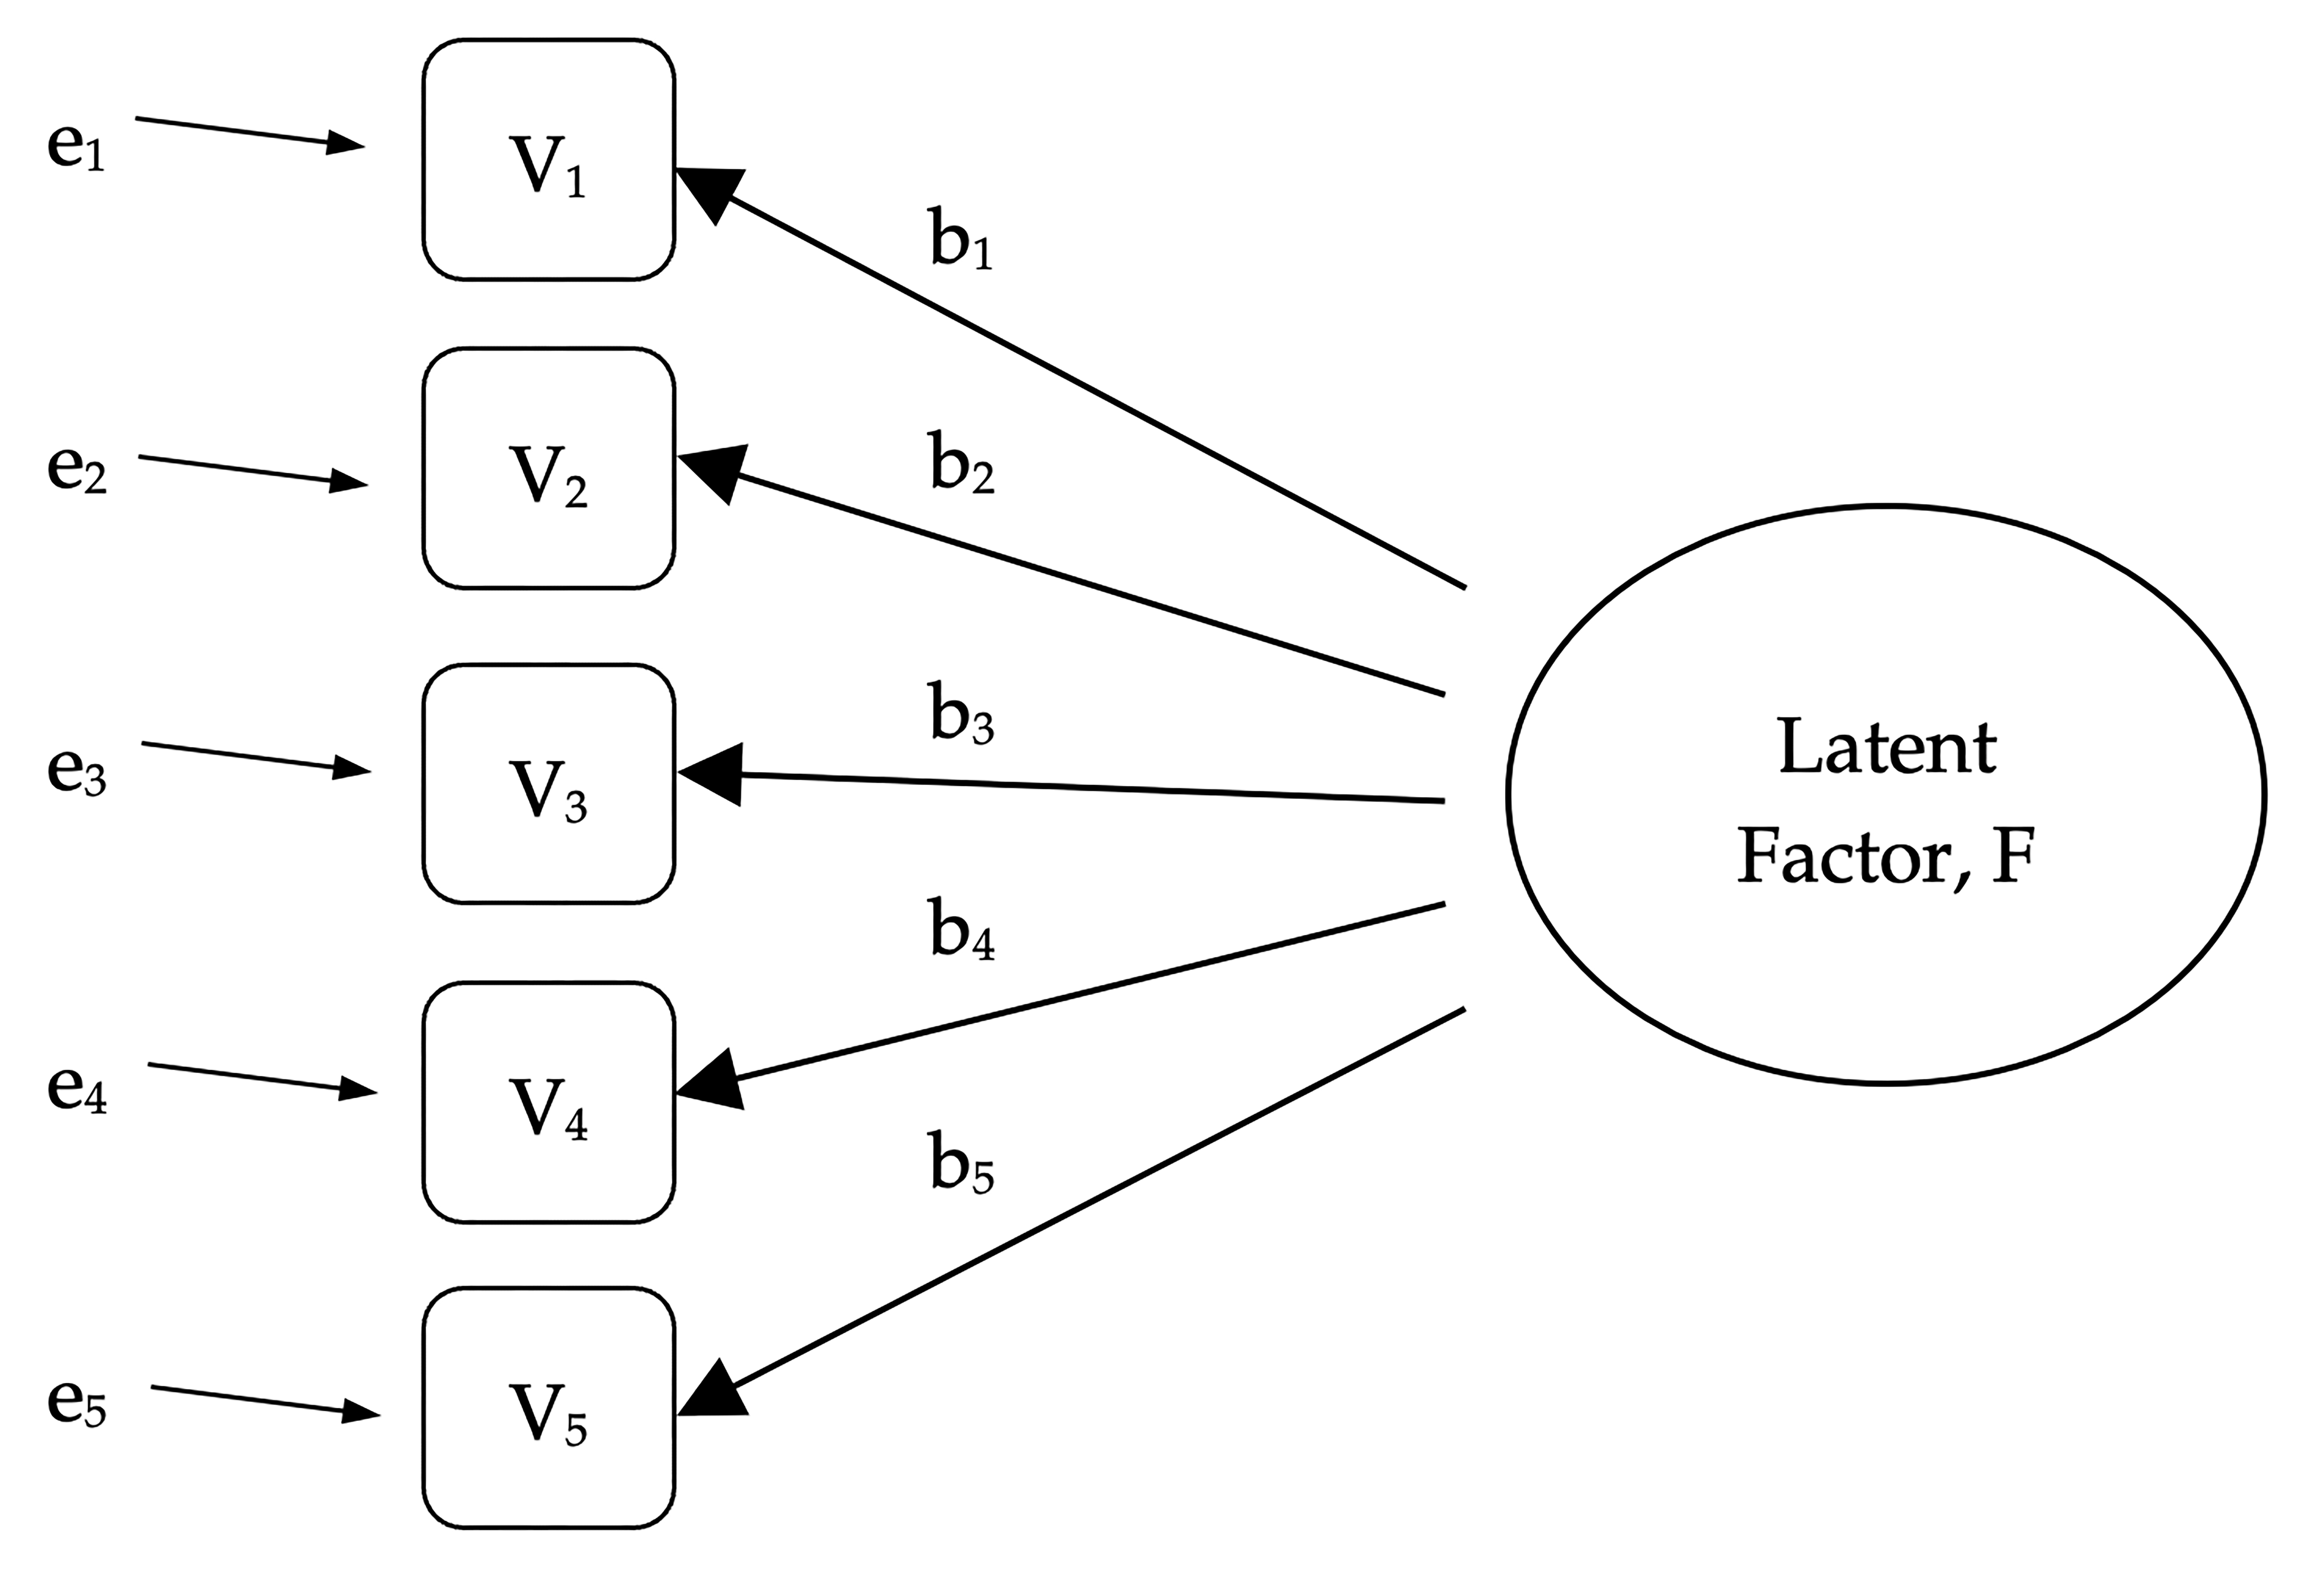
\includegraphics[width=1\textwidth,height=\textheight]{images/fig15-1.png} \hfill{}

\caption{\label{fig-fig15-1}Latent factor underlying the relationship
between several observed variables}

\end{figure}

In Psychology, latent factors represent psychological phenomena or
constructs that are difficult to directly observe or measure. For
example, personality, or intelligence, or thinking style. In the example
in Figure~\ref{fig-fig15-1} we may have asked people five specific
questions about their behaviour or attitudes, and from that we are able
to get a picture about a personality construct called, for example,
extraversion. A different set of specific questions may give us a
picture about an individual's introversion, or their conscientiousness.

Here's another example: we may not be able to directly measure
statistics anxiety, but we can measure whether statistics anxiety is
high or low with a set of questions in a questionnaire. For example,
``\(Q1\): Doing the assignment for a statistics course'', ``\(Q2\):
Trying to understand the statistics described in a journal article'',
and ``\(Q3\): Asking the lecturer for help in understanding something
from the course'', etc., each rated from low anxiety to high anxiety.
People with high statistics anxiety will tend to give similarly high
responses on these observed variables because of their high statistics
anxiety. Likewise, people with low statistics anxiety will give similar
low responses to these variables because of their low statistics
anxiety.

In exploratory factor analysis (EFA), we are essentially exploring the
correlations between observed variables to uncover any interesting,
important underlying (latent) factors that are identified when observed
variables co-vary. We can use statistical software to estimate any
latent factors and to identify which of our variables have a high
loading\footnote{Quite helpfully, factor loadings can be interpreted
  like standardized regression coefficients} (e.g.~loading
\textgreater{} 0.5) on each factor, suggesting they are a useful
measure, or indicator, of the latent factor. Part of this process
includes a step called rotation, which to be honest is a pretty weird
idea but luckily we don't have to worry about understanding it; we just
need to know that it is helpful because it makes the pattern of loadings
on different factors much clearer. As such, rotation helps with seeing
more clearly which variables are linked substantively to each factor. We
also need to decide how many factors are reasonable given our data, and
helpful in this regard is something called Eigen values. We'll come back
to this in a moment, after we have covered some of the main assumptions
of EFA.

\hypertarget{checking-assumptions}{%
\subsection{Checking assumptions}\label{checking-assumptions}}

There are a couple of assumptions that need to be checked as part of the
analysis. The first assumption is \textbf{sphericity}, which essentially
checks that the variables in your dataset are correlated with each other
to the extent that they can potentially be summarised with a smaller set
of factors. Bartlett's test for sphericity checks whether the observed
correlation matrix diverges significantly from a zero (or null)
correlation matrix. So, if Bartlett's test is significant (\(p < .05\)),
this indicates that the observed correlation matrix is significantly
divergent from the null, and is therefore suitable for EFA.

The second assumption is \textbf{sampling adequacy} and is checked using
the Kaiser-MeyerOlkin (KMO) Measure of Sampling Adequacy (MSA). The KMO
index is a measure of the proportion of variance among observed
variables that might be common variance. Using partial correlations, it
checks for factors that load just two items. We seldom, if ever, want
EFA producing a lot of factors loading just two items each. KMO is about
sampling adequacy because partial correlations are typically seen with
inadequate samples. If the KMO index is high (\(\approx 1\)), the EFA is
efficient whereas if KMO is low (\(\approx 0\)), the EFA is not
relevant. KMO values smaller than \(0.5\) indicates that EFA is not
suitable and a KMO value of \(0.6\) should be present before EFA is
considered suitable. Values between \(0.5\) and \(0.7\) are considered
adequate, values between \(0.7\) and \(0.9\) are good and values between
\(0.9\) and \(1.0\) are excellent.

\hypertarget{what-is-efa-good-for}{%
\subsection{What is EFA good for?}\label{what-is-efa-good-for}}

If the EFA has provided a good solution (i.e.~factor model), then we
need to decide what to do with our shiny new factors. Researchers often
use EFA during psychometric scale development. They will develop a pool
of questionnaire items that they think relate to one or more
psychological constructs, use EFA to see which items ``go together'' as
latent factors, and then they will assess whether some items should be
removed because they don't usefully or distinctly measure one of the
latent factors.

In line with this approach, another consequence of EFA is to combine the
variables that load onto distinct factors into a factor score, sometimes
known as a scale score. There are two options for combining variables
into a scale score:

\begin{itemize}
\tightlist
\item
  Create a new variable with a score weighted by the factor loadings for
  each item that contributes to the factor.
\item
  Create a new variable based on each item that contributes to the
  factor, but weighting them equally.
\end{itemize}

In the first option each item's contribution to the combined score
depends on how strongly it relates to the factor. In the second option
we typically just average across all the items that contribute
substantively to a factor to create the combined scale score variable.
Which to choose is a matter of preference, though a disadvantage with
the first option is that loadings can vary quite a bit from sample to
sample, and in behavioural and health sciences we are often interested
in developing and using composite questionnaire scale scores across
different studies and different samples. In which case it is reasonable
to use a composite measure that is based on the substantive items
contributing equally rather than weighting by sample specific loadings
from a different sample. In any case, understanding a combined variable
measure as an average of items is simpler and more intuitive than using
a sample specific optimally-weighted combination.

A more advanced statistical technique, one which is beyond the scope of
this book, undertakes regression modelling where latent factors are used
in prediction models of other latent factors. This is called
``structural equation modelling'' and there are specific software
programmes and R packages dedicated to this approach. But let's not get
ahead of ourselves; what we should really focus on now is how to do an
EFA in jamovi.

\hypertarget{efa-in-jamovi}{%
\subsection{EFA in jamovi}\label{efa-in-jamovi}}

First, we need some data. Twenty-five personality self-report items (see
Figure~\ref{fig-fig15-2}) taken from the International Personality Item
Pool were included as part of the Synthetic Aperture Personality
Assessment (SAPA) web-based personality assessment (SAPA:
http://sapa-project.org) project. The 25 items are organized by five
putative factors: Agreeableness, Conscientiousness, Extraversion,
Neuroticism, and Openness.

The item data were collected using a 6-point response scale:

\begin{enumerate}
\def\labelenumi{\arabic{enumi}.}
\tightlist
\item
  Very Inaccurate
\item
  Moderately Inaccurate
\item
  Slightly Inaccurate
\item
  Slightly Accurate
\item
  Moderately Accurate
\item
  Very Accurate.
\end{enumerate}

A sample of \(N=250\) responses is contained in the dataset
\emph{bfi\_sample.csv} . As researchers, we are interested in exploring
the data to see whether there are some underlying latent factors that
are measured reasonably well by the \(25\) observed variables in the
\emph{bfi\_sample.csv} data file. Open up the dataset and check that the
\(25\) variables are coded as continuous variables (technically they are
ordinal though for EFA in jamovi it mostly doesn't matter, except if you
decide to calculate weighted factor scores in which case continuous
variables are needed). To perform EFA in jamovi:

\begin{figure}

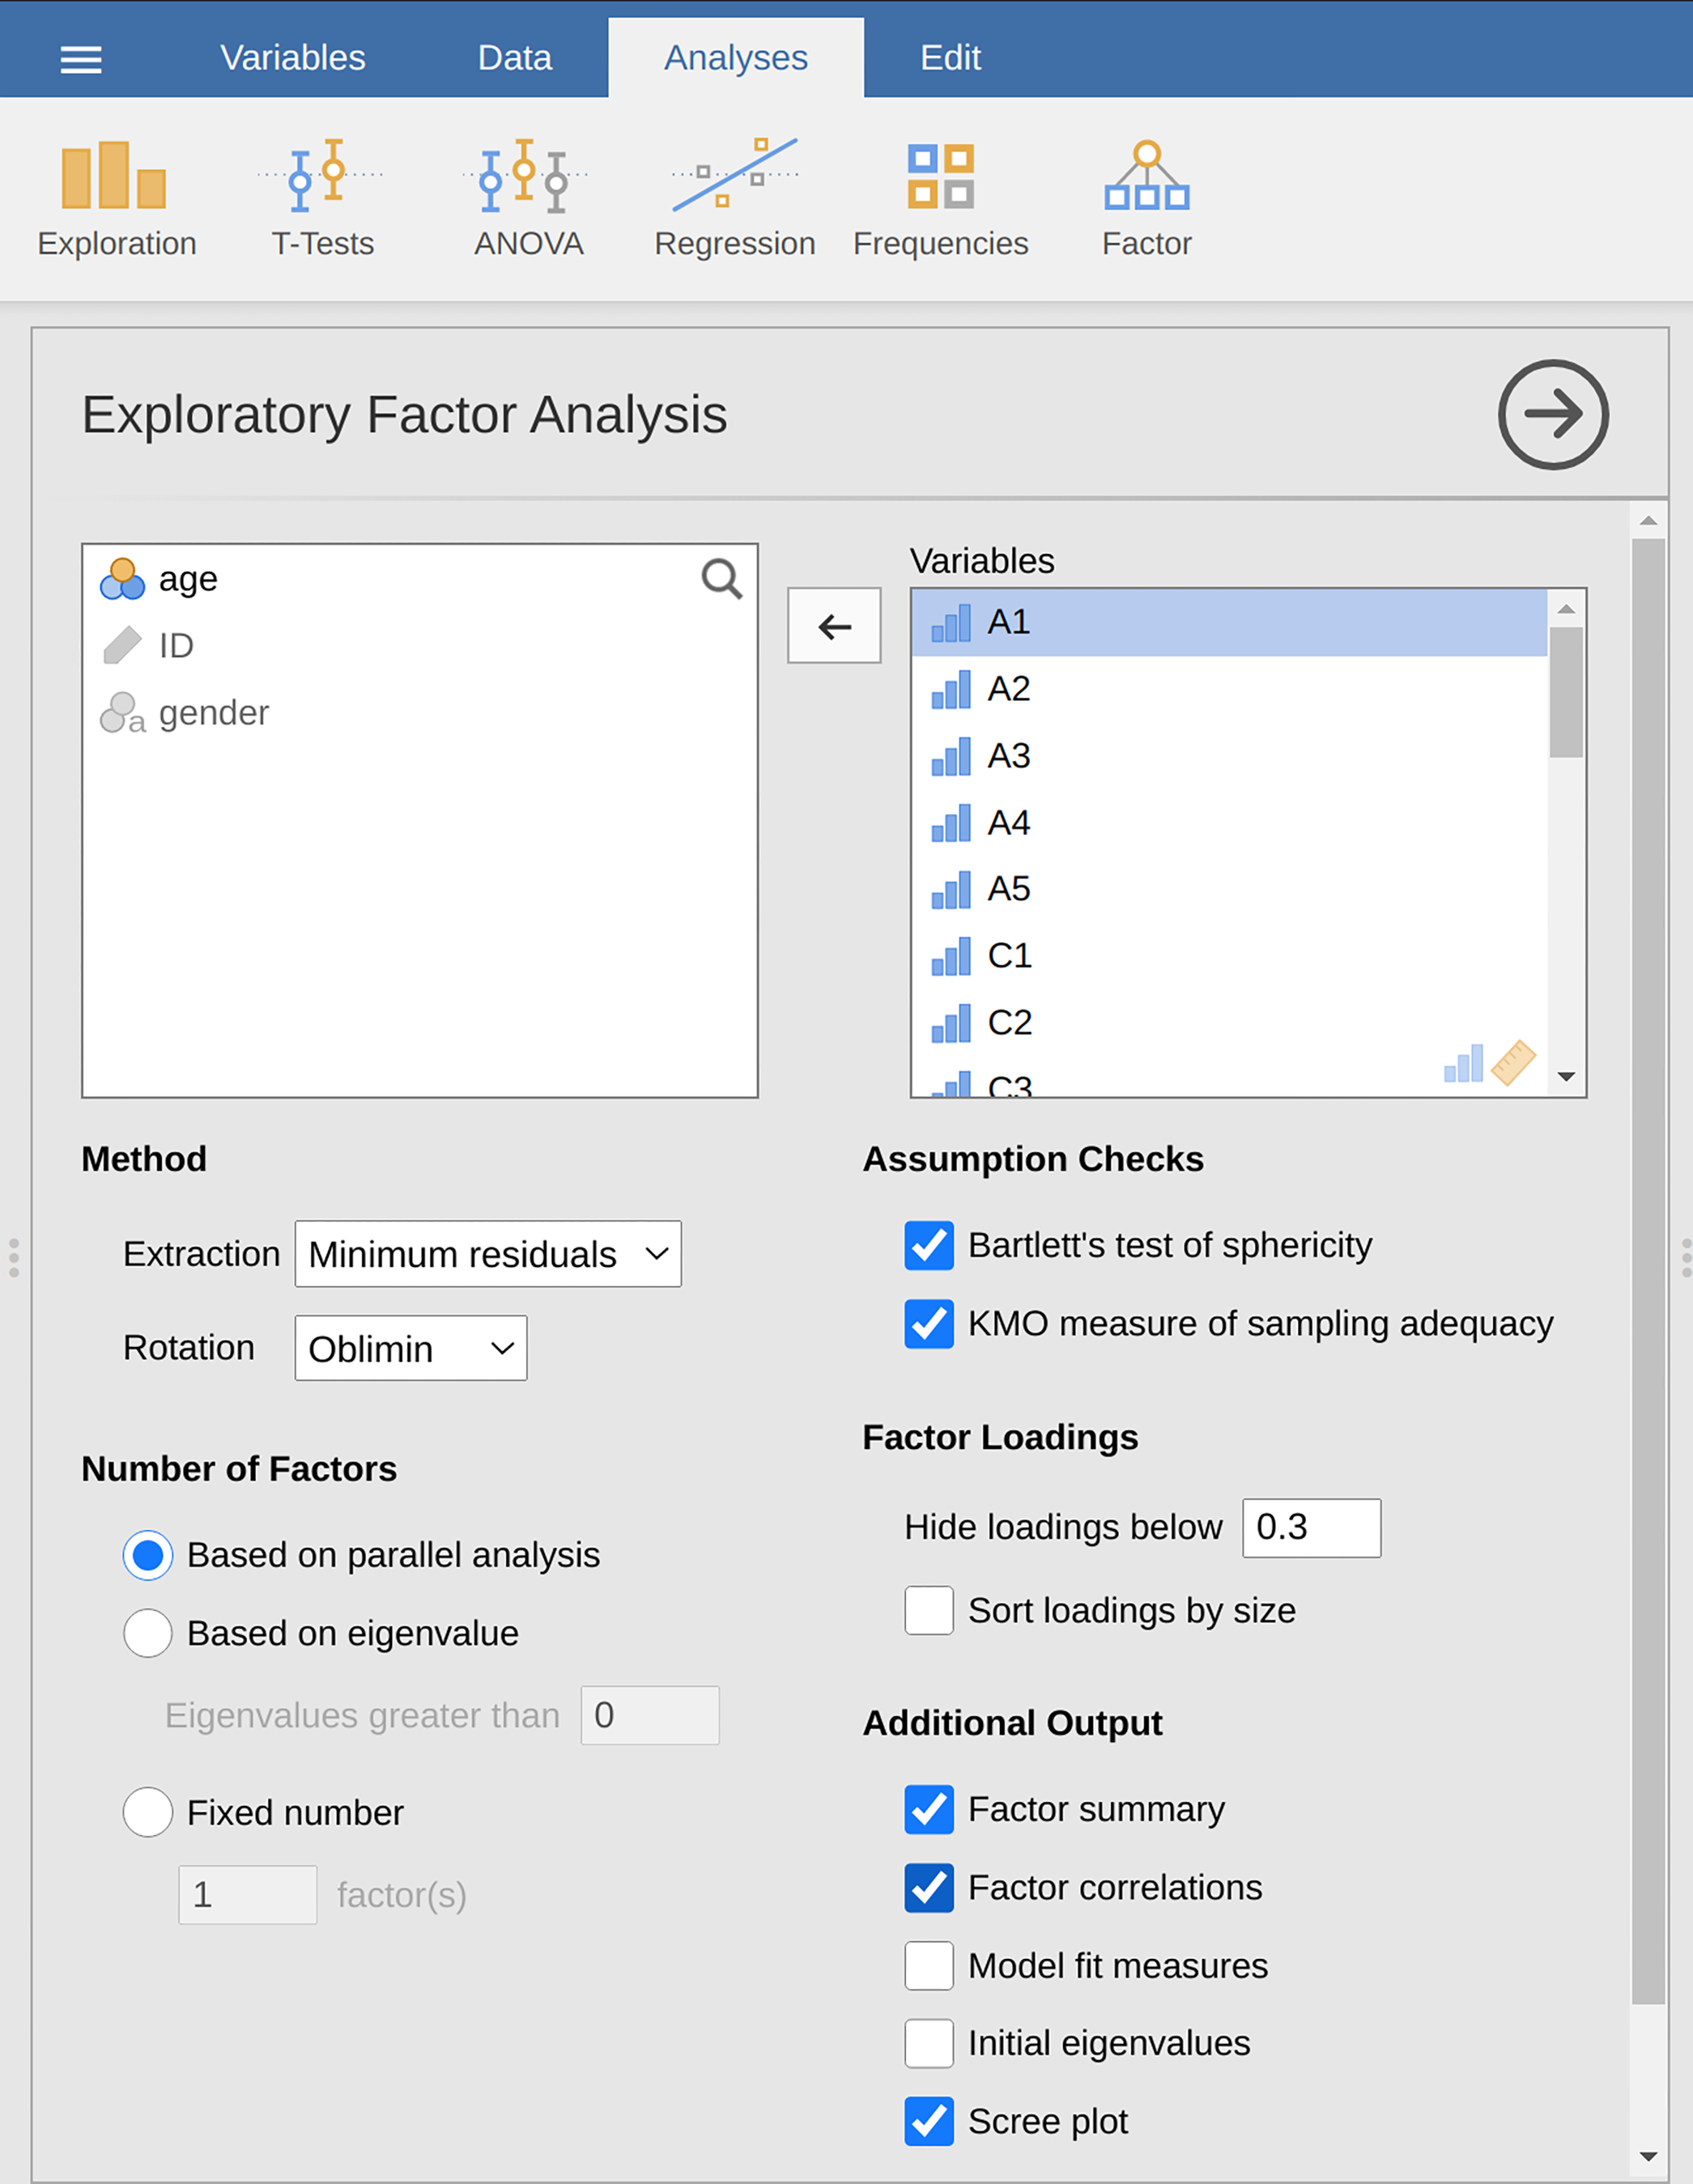
\includegraphics[width=1\textwidth,height=\textheight]{images/fig15-2.png} \hfill{}

\caption{\label{fig-fig15-2}Twenty-five observed variable items
organised by five putative personality factors in the dataset
bfi\_sample.csv}

\end{figure}

\begin{itemize}
\item
  Select Factor - Exploratory Factor Analysis from the main jamovi
  button bar to open the EFA analysis window (Figure~\ref{fig-fig15-3}).
\item
  Select the 25 personality questions and transfer them into the
  `Variables' box.
\item
  Check appropriate options, including `Assumption Checks', but also
  Rotation `Method', `Number of Factors' to extract, and `Additional
  Output' options. See Figure~\ref{fig-fig15-3} for suggested options
  for this illustrative EFA, and please note that the Rotation `Method'
  and `Number of Factors' extracted is typically adjusted by the
  researcher during the analysis to find the best result, as described
  below.
\end{itemize}

\begin{figure}

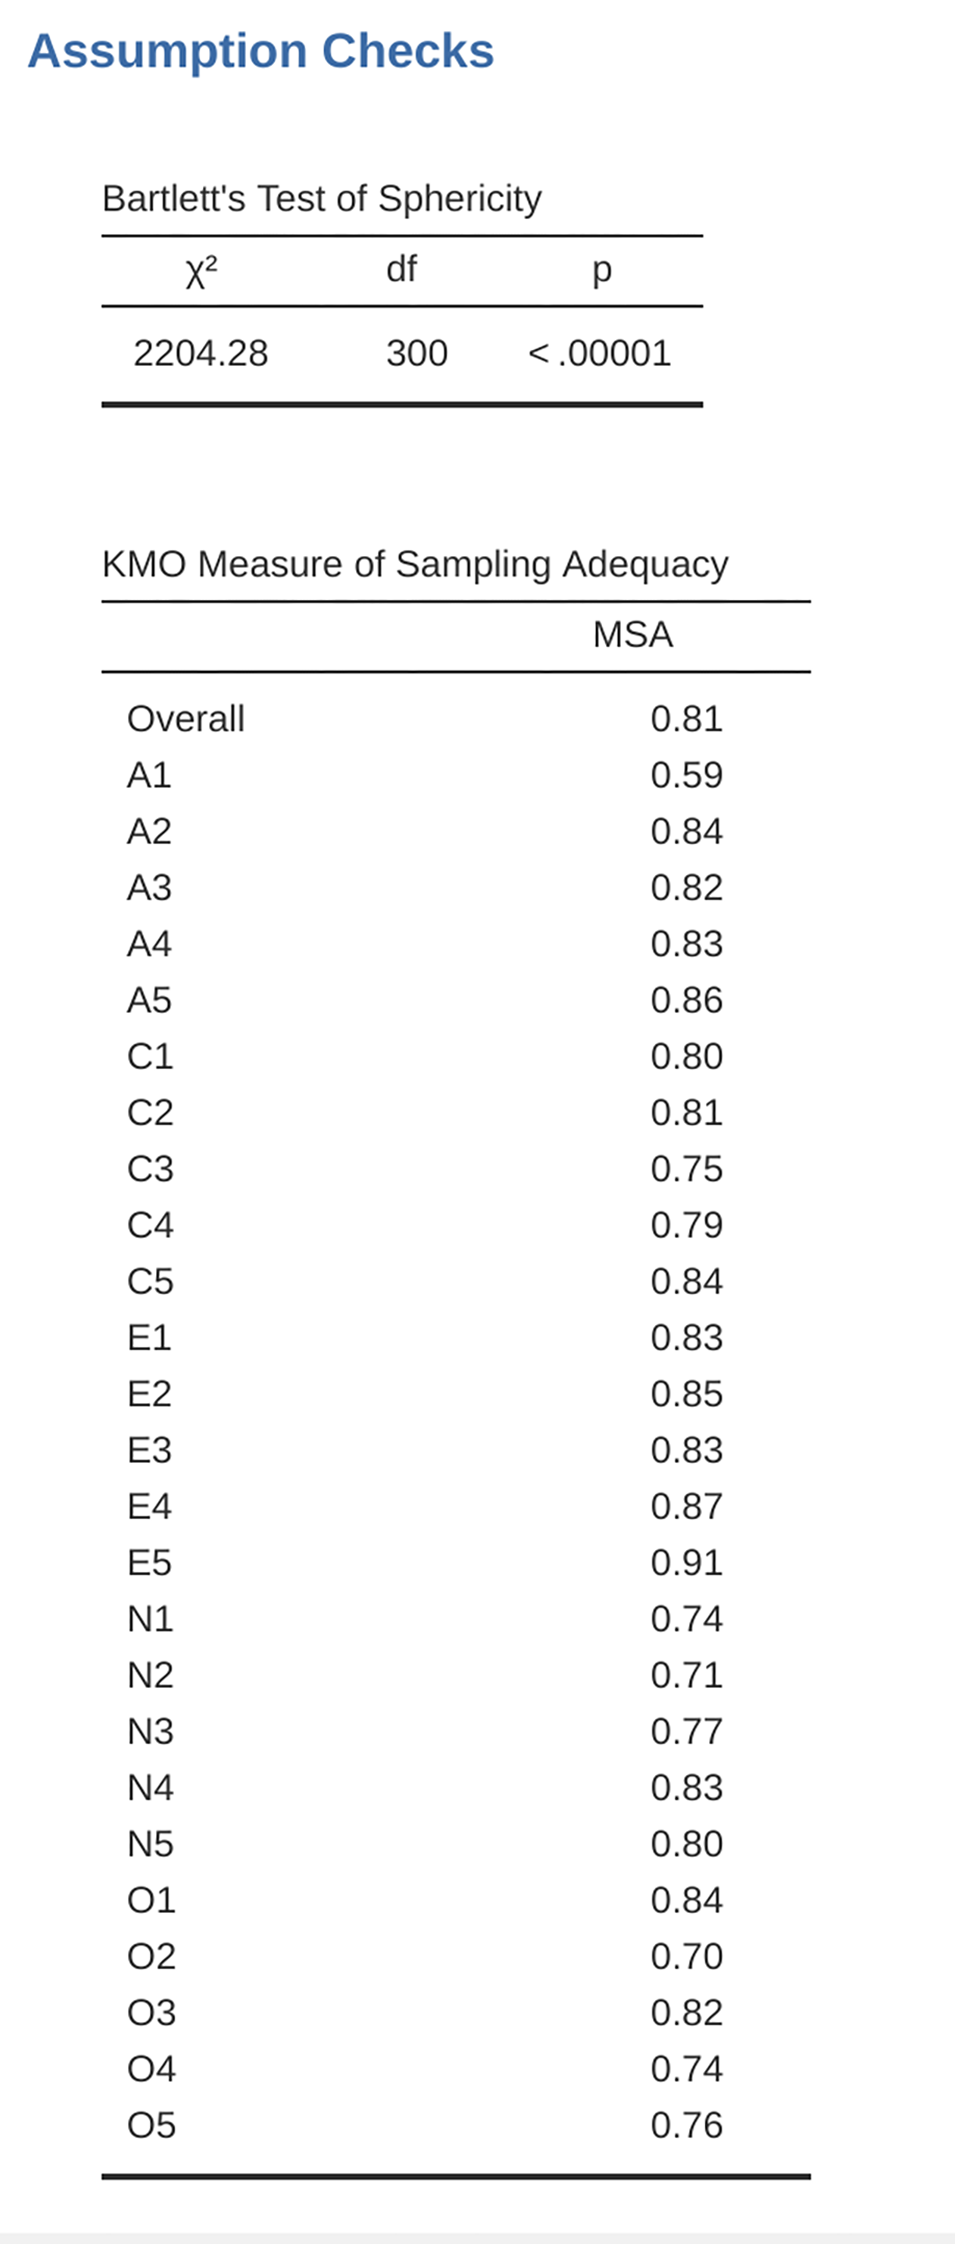
\includegraphics[width=1\textwidth,height=\textheight]{images/fig15-3.png} \hfill{}

\caption{\label{fig-fig15-3}The jamovi EFA analysis window}

\end{figure}

\begin{figure}

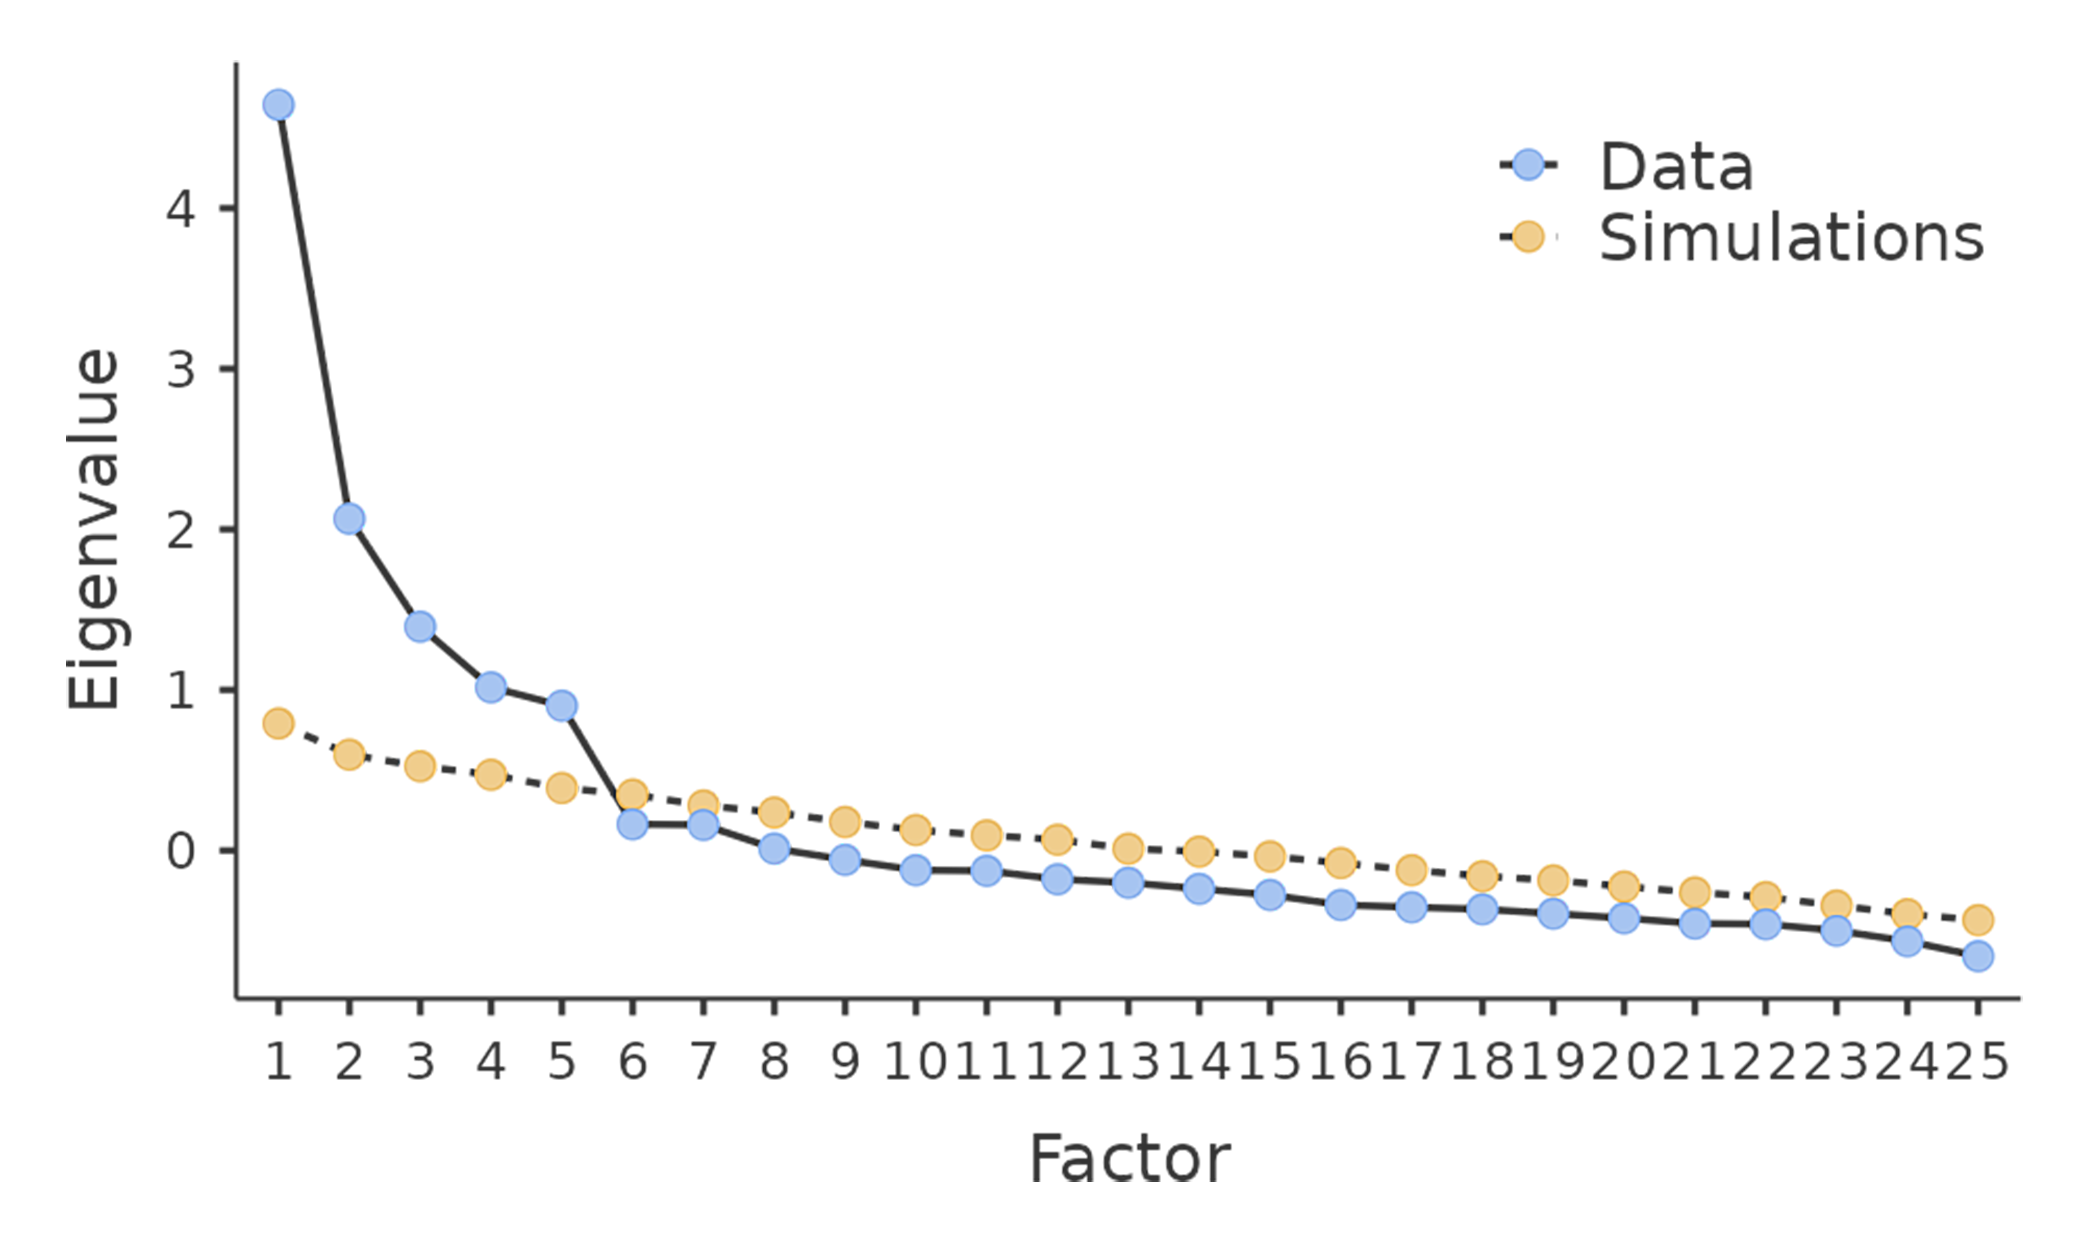
\includegraphics[width=1\textwidth,height=\textheight]{images/fig15-4.png} \hfill{}

\caption{\label{fig-fig15-4}jamovi EFA assumption checks for the
personality questionnaire data}

\end{figure}

First, check the assumptions (Figure~\ref{fig-fig15-4}). You can see
that (1) Bartlett's test of sphericity is significant, so this
assumption is satisfied; and (2) the KMO measure of sampling adequacy
(MSA) is \(0.81\) overall, suggesting good sampling adequacy. No
problems here then!

The next thing to check is how many factors to use (or ``extract'' from
the data). Three different approaches are available:

\begin{itemize}
\tightlist
\item
  One convention is to choose all components with Eigen values greater
  than 1\footnote{An Eigen value indicates how much of the variance in
    the observed variables a factor accounts for. A factor with an Eigen
    value \textgreater{} 1 accounts for more variance than a single
    observed variable.}. This would give us four factors with our data
  (try it and see).
\end{itemize}

\begin{itemize}
\item
  Examination of the scree plot, as in Figure~\ref{fig-fig15-5}, lets
  you identify the ``point of inflection''. This is the point at which
  the slope of the scree curve clearly levels off, below the ``elbow''.
  This would give us five factors with our data. Interpreting scree
  plots is a bit of an art: in Figure~\ref{fig-fig15-5} there is a
  noticeable step from \(5\) to \(6\) factors, but in other scree plots
  you look at it will not be so clear cut.
\item
  Using a parallel analysis technique, the obtained Eigen values are
  compared to those that would be obtained from random data. The number
  of factors extracted is the number with Eigen values greater than what
  would be found with random data.
\end{itemize}

\begin{figure}

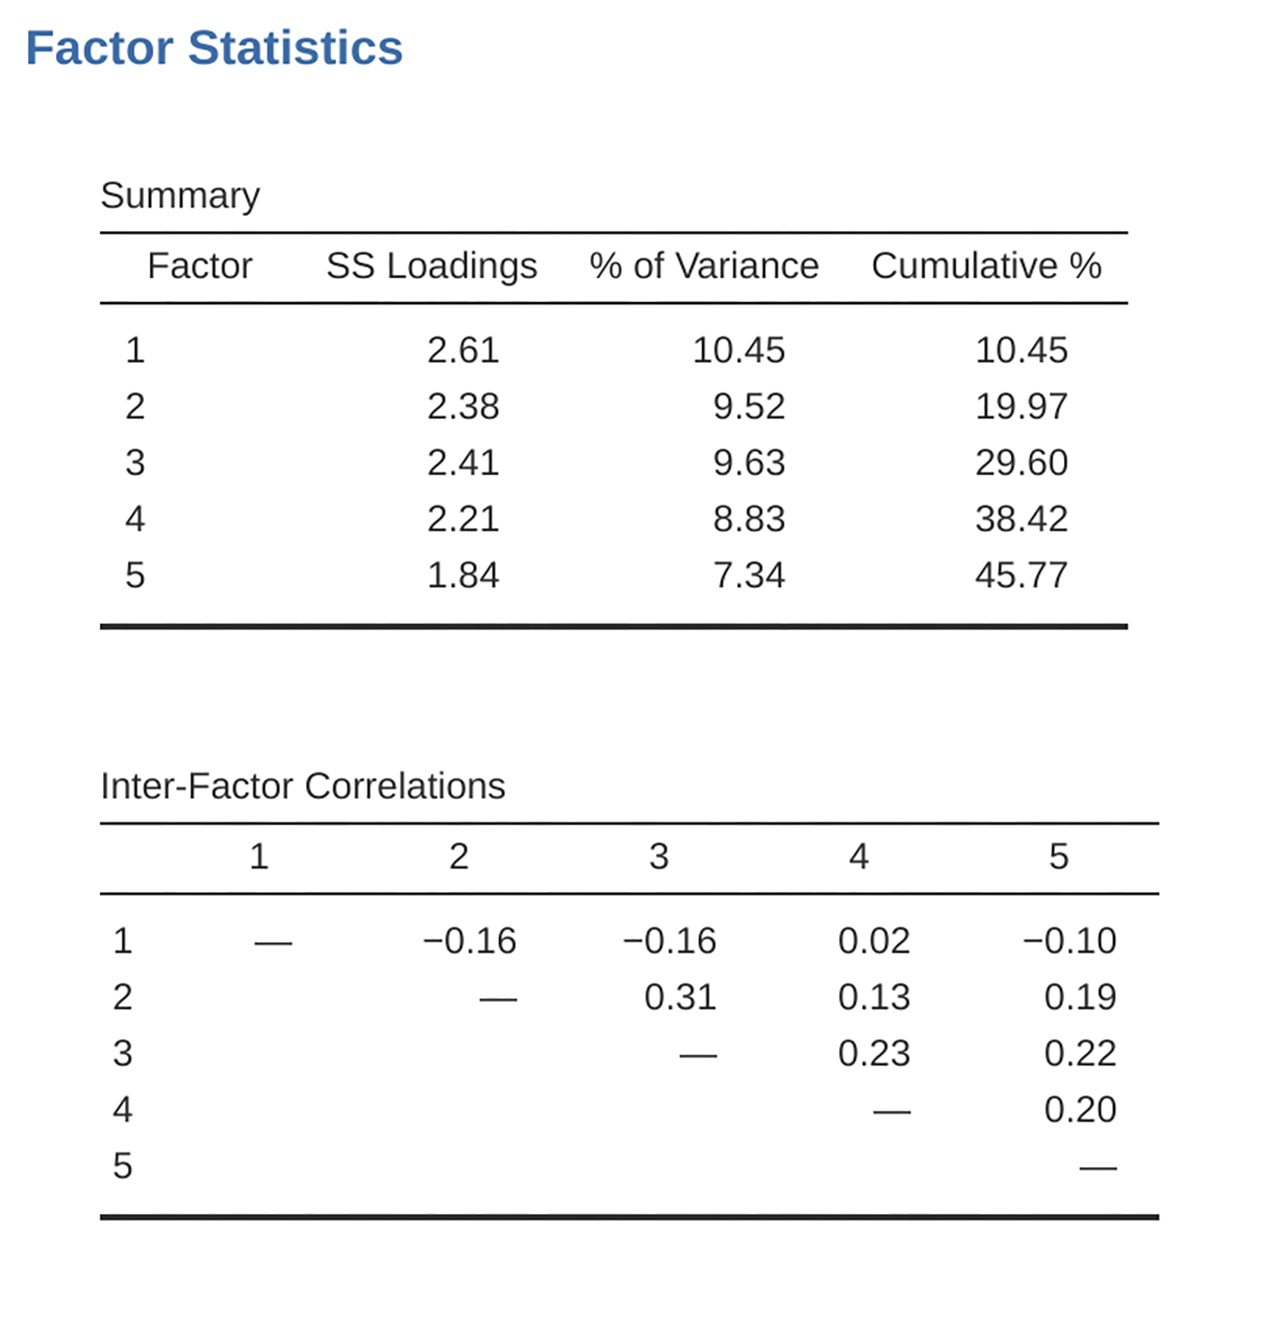
\includegraphics[width=1\textwidth,height=\textheight]{images/fig15-5.png} \hfill{}

\caption{\label{fig-fig15-5}Scree plot of the personality data in jamovi
EFA, showing a noticeable inflection and levelling off after point 5
(the `elbow')}

\end{figure}

The third approach is a good one according to Fabrigar et al. (1999),
although in practice researchers tend to look at all three and then make
a judgement about the number of factors that are most easily or
helpfully interpreted. This can be understood as the ``meaningfulness
criterion'', and researchers will typically examine, in addition to the
solution from one of the approaches above, solutions with one or two
more or fewer factors. They then adopt the solution which makes the most
sense to them.

At the same time, we should also consider the best way to rotate the
final solution. There are two main approaches to rotation: orthogonal
(e.g.~`varimax') rotation forces the selected factors to be
uncorrelated, whereas oblique (e.g.~`oblimin') rotation allows the
selected factors to be correlated. Dimensions of interest to
psychologists and behavioural scientists are not often dimensions we
would expect to be orthogonal, so oblique solutions are arguably more
sensible\footnote{Oblique rotations provide two factor matrices, one
  called a structure matrix and one called a pattern matrix. In jamovi
  just the pattern matrix is shown in the results as this is typically
  the most useful for interpretation, though some experts suggest that
  both can be helpful. In a structure matrix coefficients show the
  relationship between the variable and the factors whilst ignoring the
  relationship of that factor with all the other factors (i.e.~a
  zero-order correlation). Pattern matrix coefficients show the unique
  contribution of a factor to a variable whilst controlling for the
  effects of other factors on that variable (akin to standardized
  partial regression coefficient). Under orthogonal rotation, structure
  and pattern coefficients are the same.}

\begin{figure}

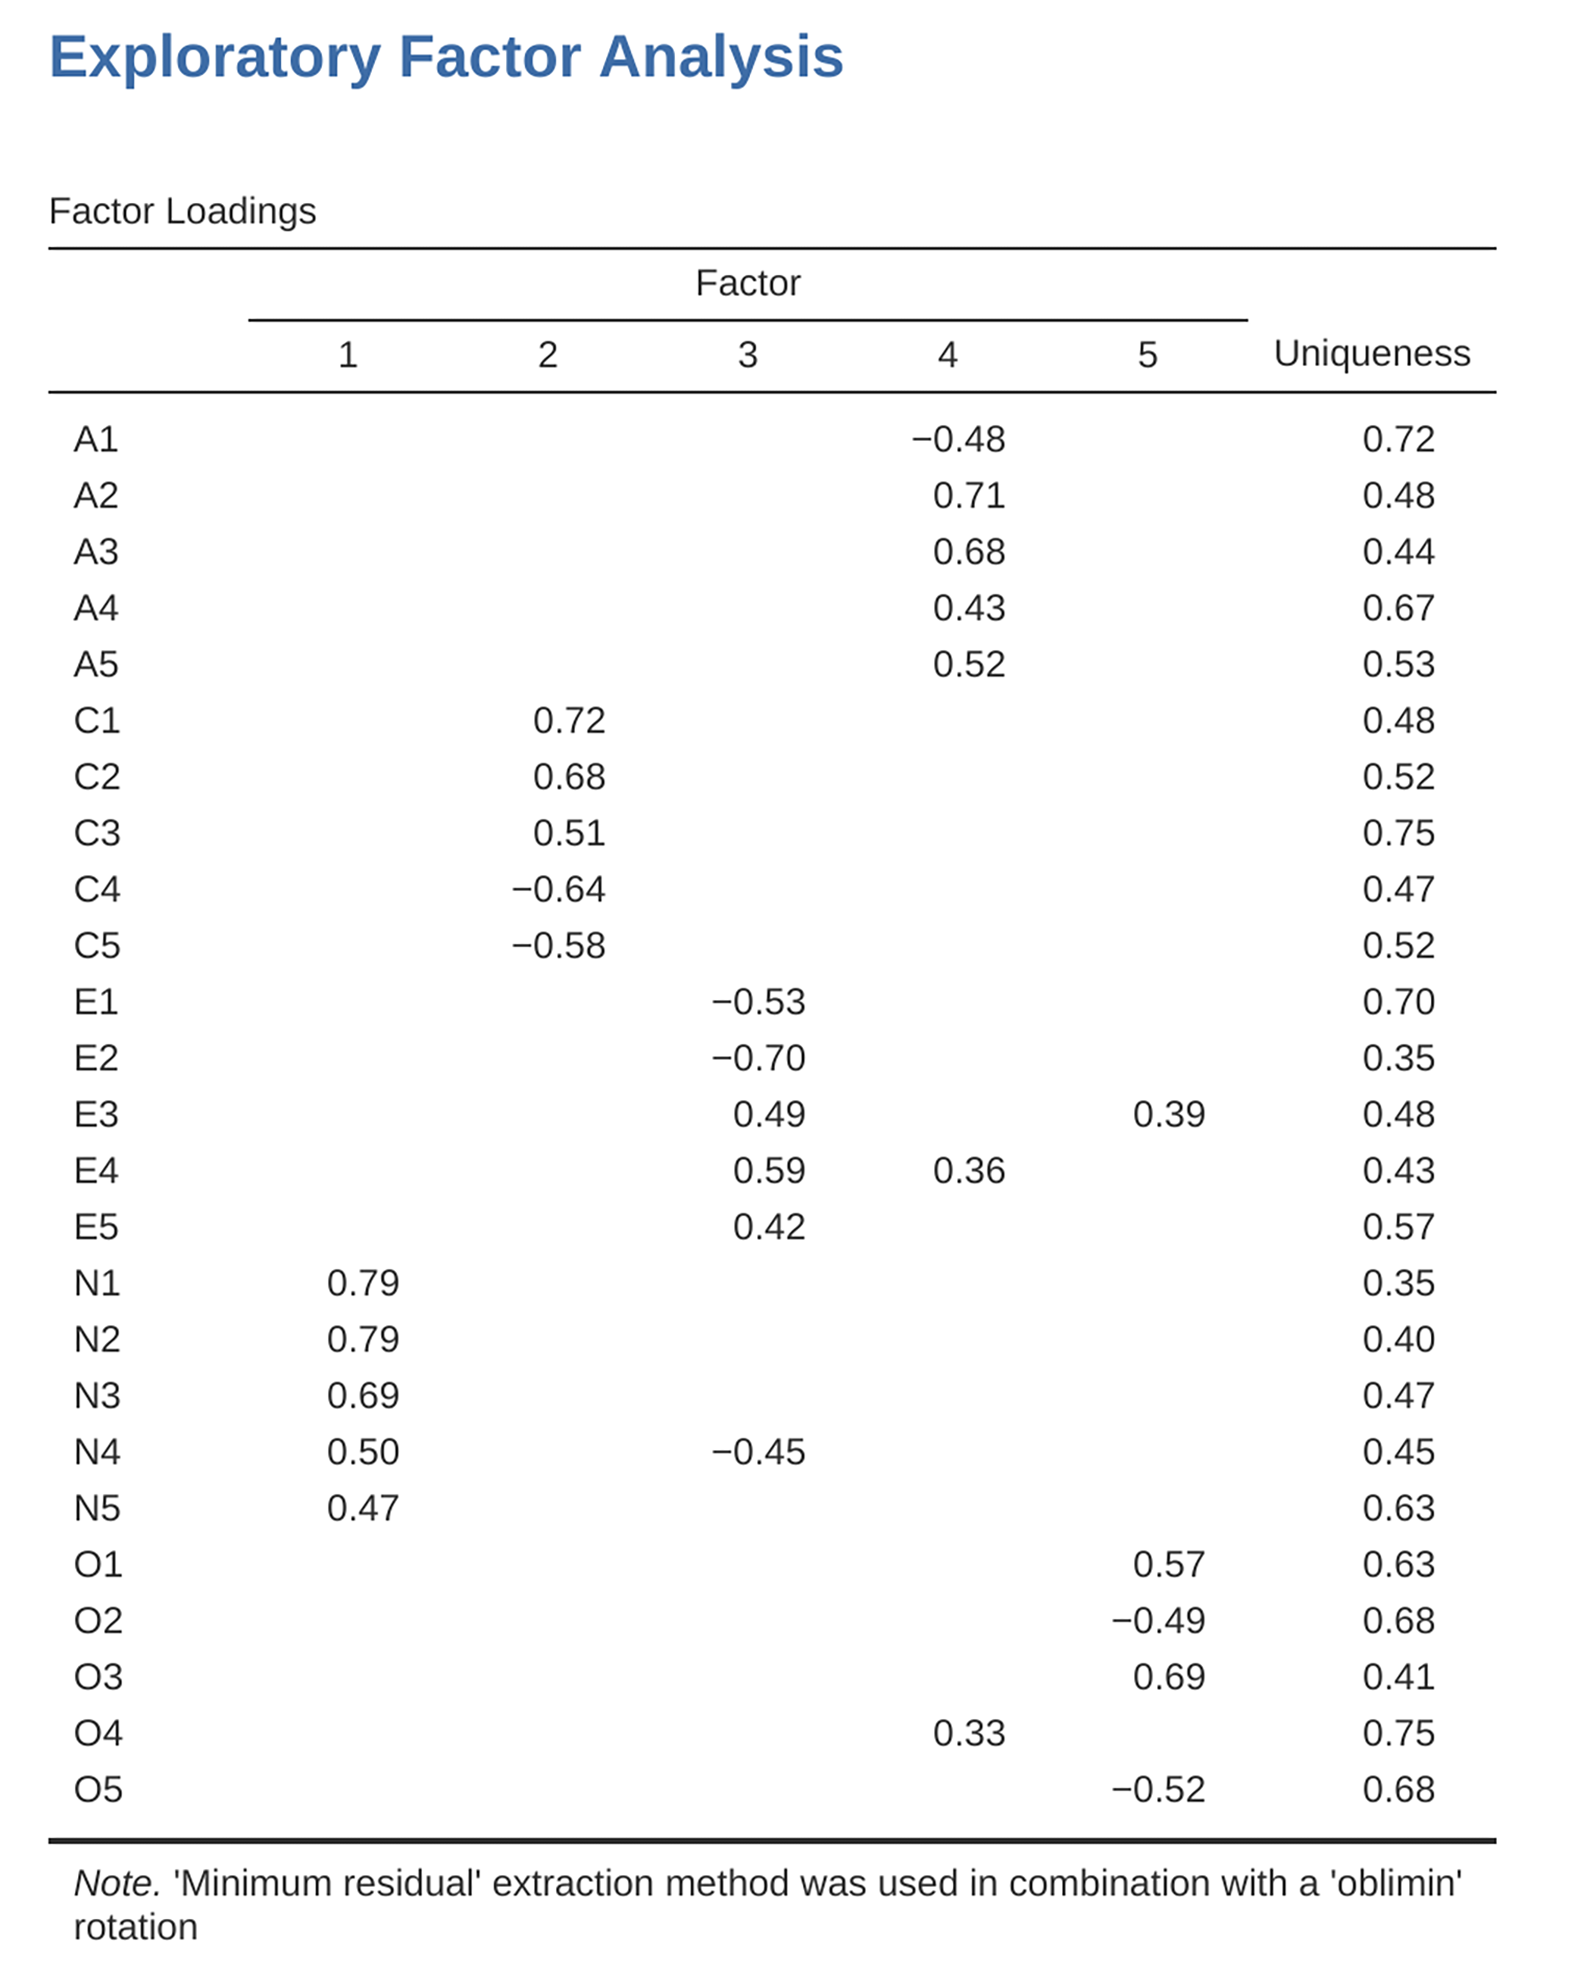
\includegraphics[width=1\textwidth,height=\textheight]{images/fig15-6.png} \hfill{}

\caption{\label{fig-fig15-6}Factor summary statistics and correlations
for a five factor solution in jamovi EFA}

\end{figure}

Practically, if in an oblique rotation the factors are found to be
substantially correlated (positive or negative, and \textgreater{} 0.3),
as in Figure~\ref{fig-fig15-6} where a correlation between two of the
extracted factors is 0.31, then this would confirm our intuition to
prefer oblique rotation. If the factors are, in fact, correlated, then
an oblique rotation will produce a better estimate of the true factors
and a better simple structure than will an orthogonal rotation. And, if
the oblique rotation indicates that the factors have close to zero
correlations between one another, then the researcher can go ahead and
conduct an orthogonal rotation (which should then give about the same
solution as the oblique rotation).

On checking the correlation between the extracted factors at least one
correlation was greater than 0.3 (Figure~\ref{fig-fig15-6}), so an
oblique (`oblimin') rotation of the five extracted factors is preferred.
We can also see in Figure~\ref{fig-fig15-6} that the proportion of
overall variance in the data that is accounted for by the five factors
is 46\%. Factor one accounts for around 10\% of the variance, factors
two to four around 9\% each, and factor five just over 7\%. This isn't
great; it would have been better if the overall solution accounted for a
more substantive proportion of the variance in our data.

Be aware that in every EFA you could potentially have the same number of
factors as observed variables, but every additional factor you include
will add a smaller amount of explained variance. If the first few
factors explain a good amount of the variance in the original 25
variables, then those factors are clearly a useful, simpler substitute
for the 25 variables. You can drop the rest without losing too much of
the original variability. But if it takes 18 factors (for example) to
explain most of the variance in those 25 variables, you might as well
just use the original 25.

Figure~\ref{fig-fig15-7} shows the factor loadings. That is, how the 25
different personality items load onto each of the five selected factors.
We have hidden loadings less than \(0.3\) (set in the options shown in
Figure~\ref{fig-fig15-3}.

For Factors \(1, 2, 3\) and \(4\) the pattern of factor loadings closely
matches the putative factors specified in Figure~\ref{fig-fig15-2}.
Phew! And factor \(5\) is pretty close, with four of the five observed
variables that putatively measure ``openness'' loading pretty well onto
the factor. Variable \(04\) doesn't quite seem to fit though, as the
factor solution in Figure~\ref{fig-fig15-7} suggests that it loads onto
factor \(4\) (albeit with a relatively low loading) but not
substantively onto factor \(5\).

The other thing to note is that those variables that were denoted as
``R: reverse coding'' in Figure~\ref{fig-fig15-2} are those that have
negative factor loadings. Take a look at the items A1 (``Am indifferent
to the feelings of others'') and A2 (``Inquire about others'
well-being''). We can see that a high score on \(A1\) indicates low
Agreeableness, whereas a high score on \(A2\) (and all the other ``A''
variables for that matter) indicates high Agreeableness. Therefore A1
will be negatively correlated with the other ``A'' variables, and this
is why it has a negative factor loading, as shown in
Figure~\ref{fig-fig15-7}.

\begin{figure}

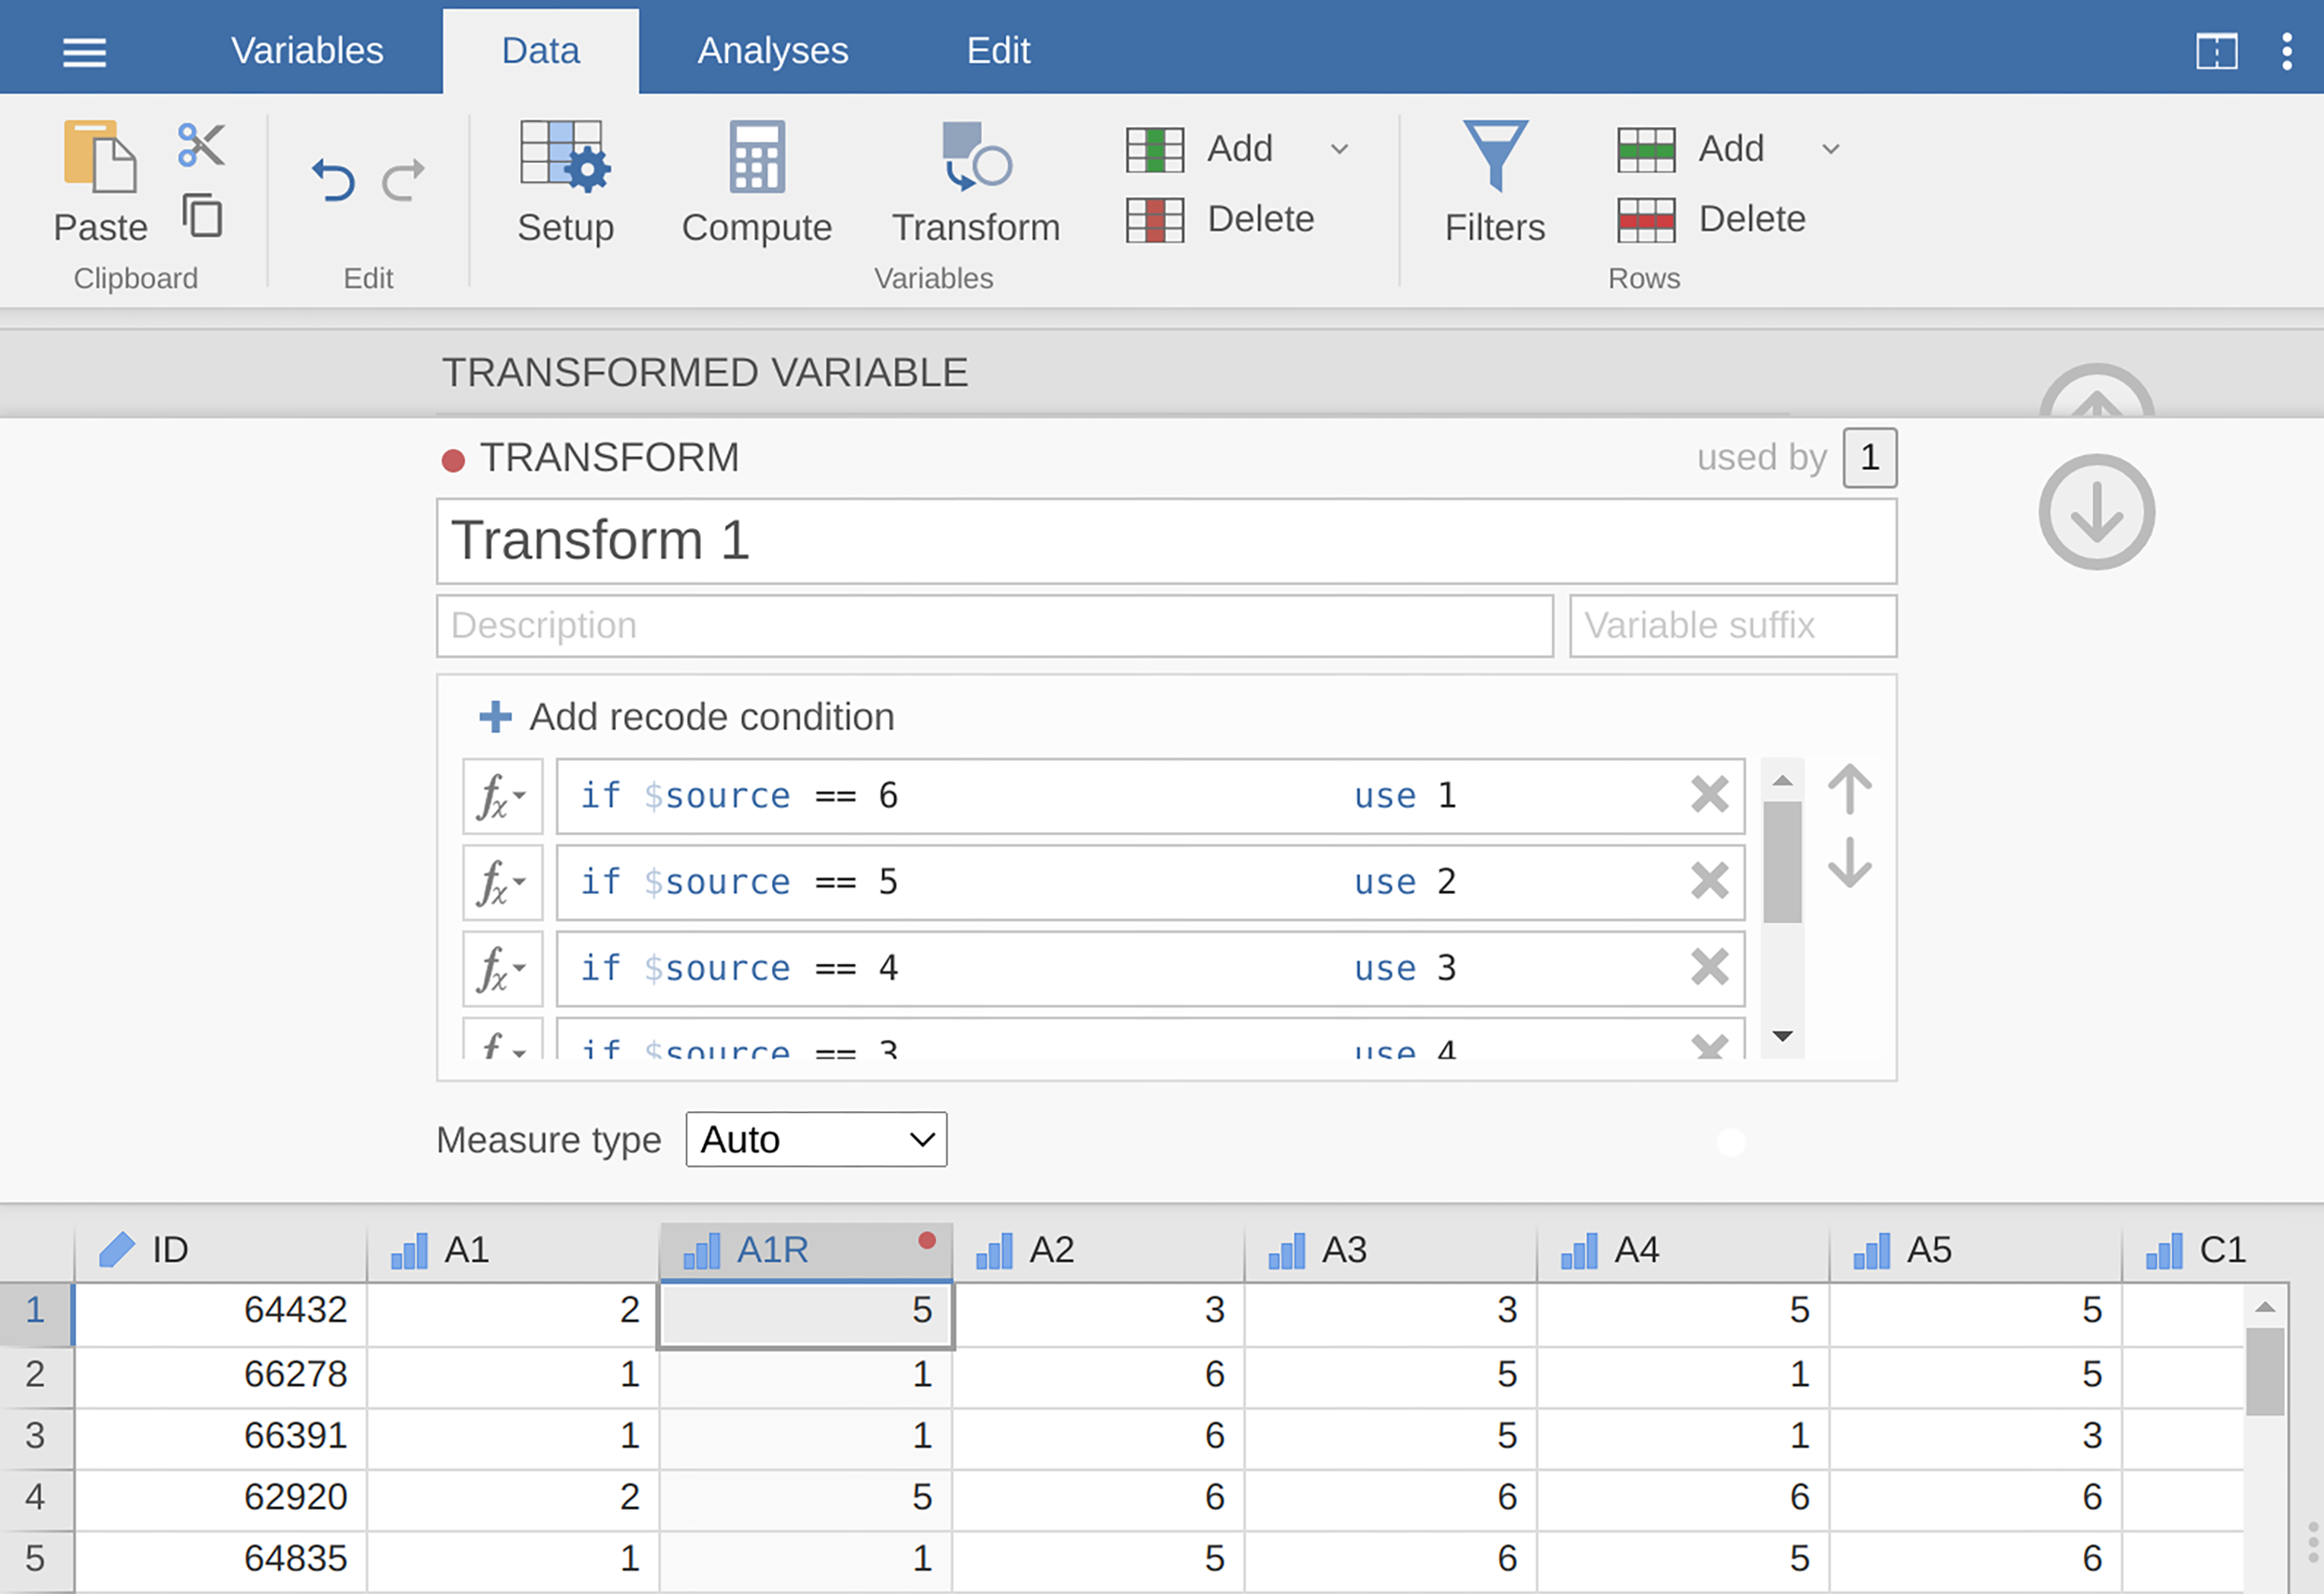
\includegraphics[width=1\textwidth,height=\textheight]{images/fig15-7.png} \hfill{}

\caption{\label{fig-fig15-7}Factor loadings for a five factor solution
in jamovi EFA}

\end{figure}

We can also see in Figure~\ref{fig-fig15-7} the ``uniqueness'' of each
variable. Uniqueness is the proportion of variance that is `unique' to
the variable and not explained by the factors\footnote{Sometimes
  reported in factor analysis is ``communality'' which is the amount of
  variance in a variable that is accounted for by the factor solution.
  Uniqueness is equal to (1 \(\sim\) communality)}. For example, 72\% of
the variance in `A1' is not explained by the factors in the five factor
solution. In contrast, `N1' has relatively low variance not accounted
for by the factor solution (35\%). Note that the greater the
`uniqueness', the lower the relevance or contribution of the variable in
the factor model.

To be honest, it's unusual to get such a neat solution in EFA. It's
typically quite a bit more messy than this, and often interpreting the
meaning of the factors is more challenging. It's not often that you have
such a clearly delineated item pool. More often you will have a whole
heap of observed variables that you think may be indicators of a few
underlying latent factors, but you don't have such a strong sense of
which variables are going to go where!

So, we seem to have a pretty good five factor solution, albeit
accounting for a relatively low overall proportion of the observed
variance. Let's assume we are happy with this solution and want to use
our factors in further analysis. The straightforward option is to
calculate an overall (average) score for each factor by adding together
the score for each variable that loads substantively onto the factor and
then dividing by the number of variables (in other words create a `mean
score' for each person across the items for each scale. For each person
in our dataset that entails, for example for the Agreeableness factor,
adding together \(A1 + A2 + A3 + A4 + A5\), and then dividing by 5.
\footnote{remembering to first reverse score some variables if necessary}
In essence, the factor score we have calculated is based on equally
weighted scores from each of the included variables/itmes. We can do
this in jamovi in two steps:

\begin{itemize}
\item
  Recode A1 into ``A1R'' by reverse scoring the values in the variable
  (i.e.~\(6 = 1\); \(5 = 2\); \(4 = 3\); \(3 = 4\); \(2 = 5\);
  \(1 = 6\)) using the jamovi transform variable command (see
  Figure~\ref{fig-fig15-8}).
\item
  Compute a new variable, called ``Agreeableness', by calculating the
  mean of A1R, A2, A3, A4 and A5. Do this using the jamovi compute new
  variable command (see Figure~\ref{fig-fig15-9}).
\end{itemize}

\begin{figure}

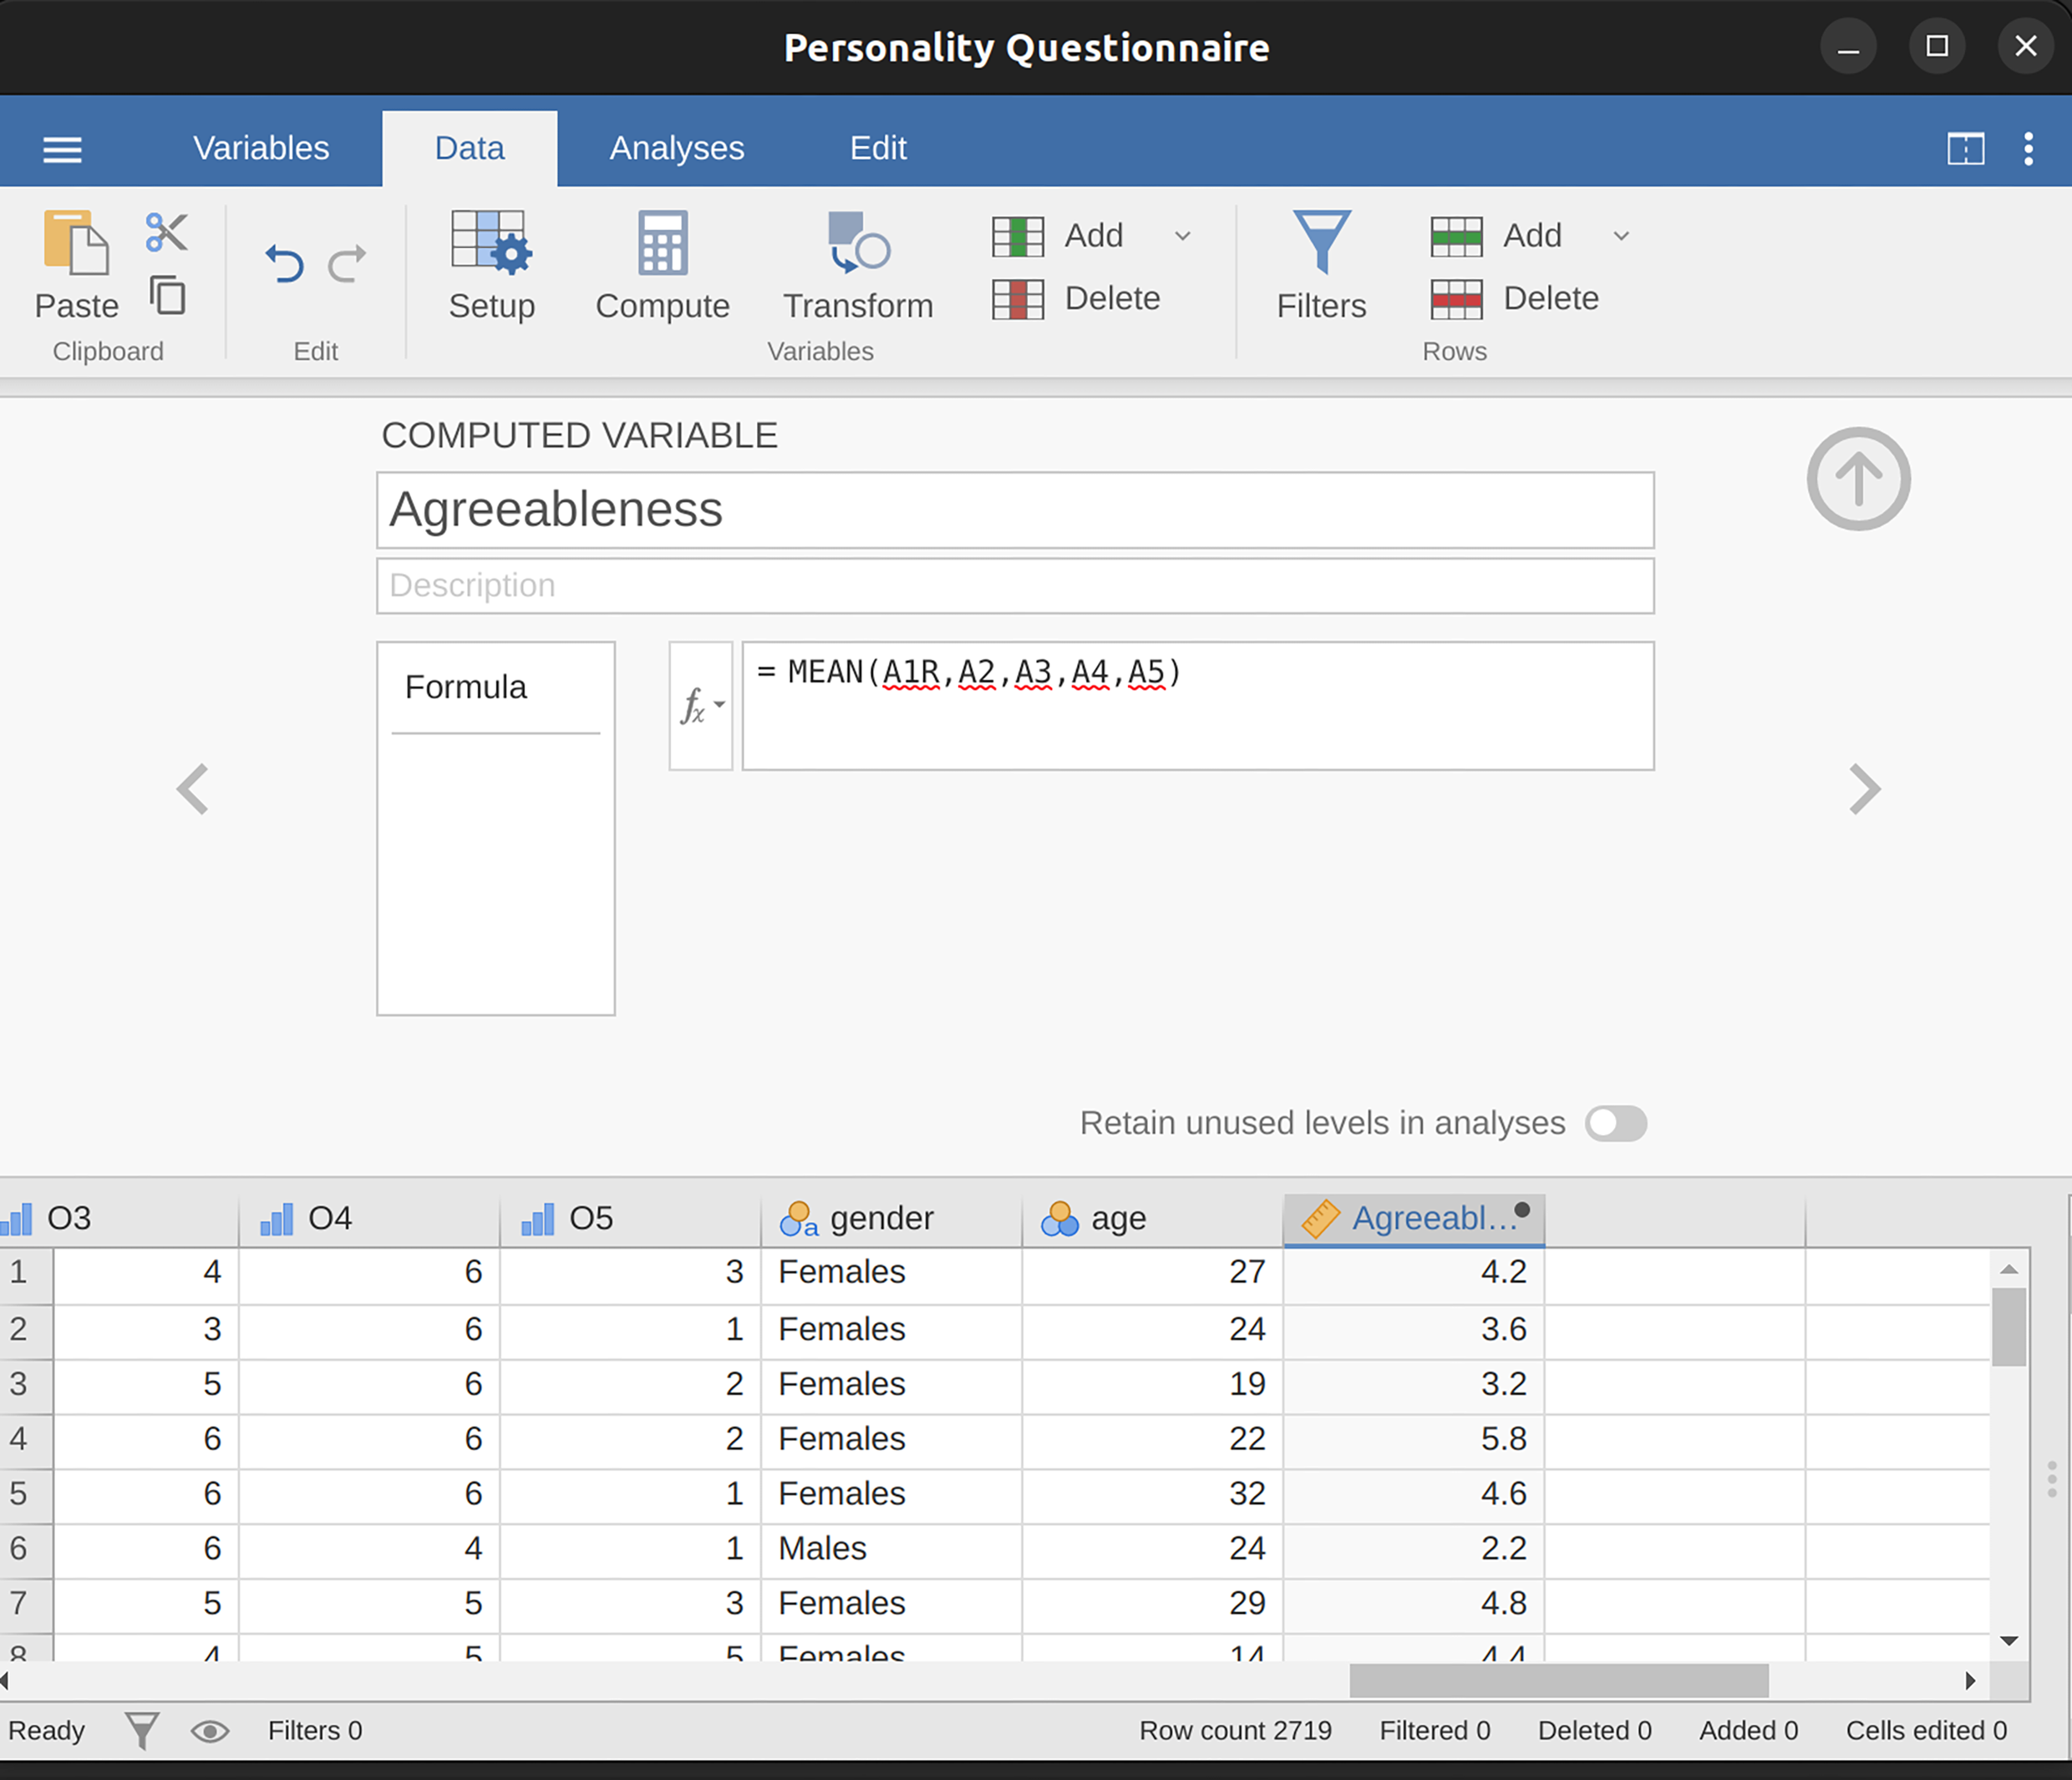
\includegraphics[width=1\textwidth,height=\textheight]{images/fig15-8.png} \hfill{}

\caption{\label{fig-fig15-8}Recode variable using the jamovi Transform
command}

\end{figure}

\begin{figure}

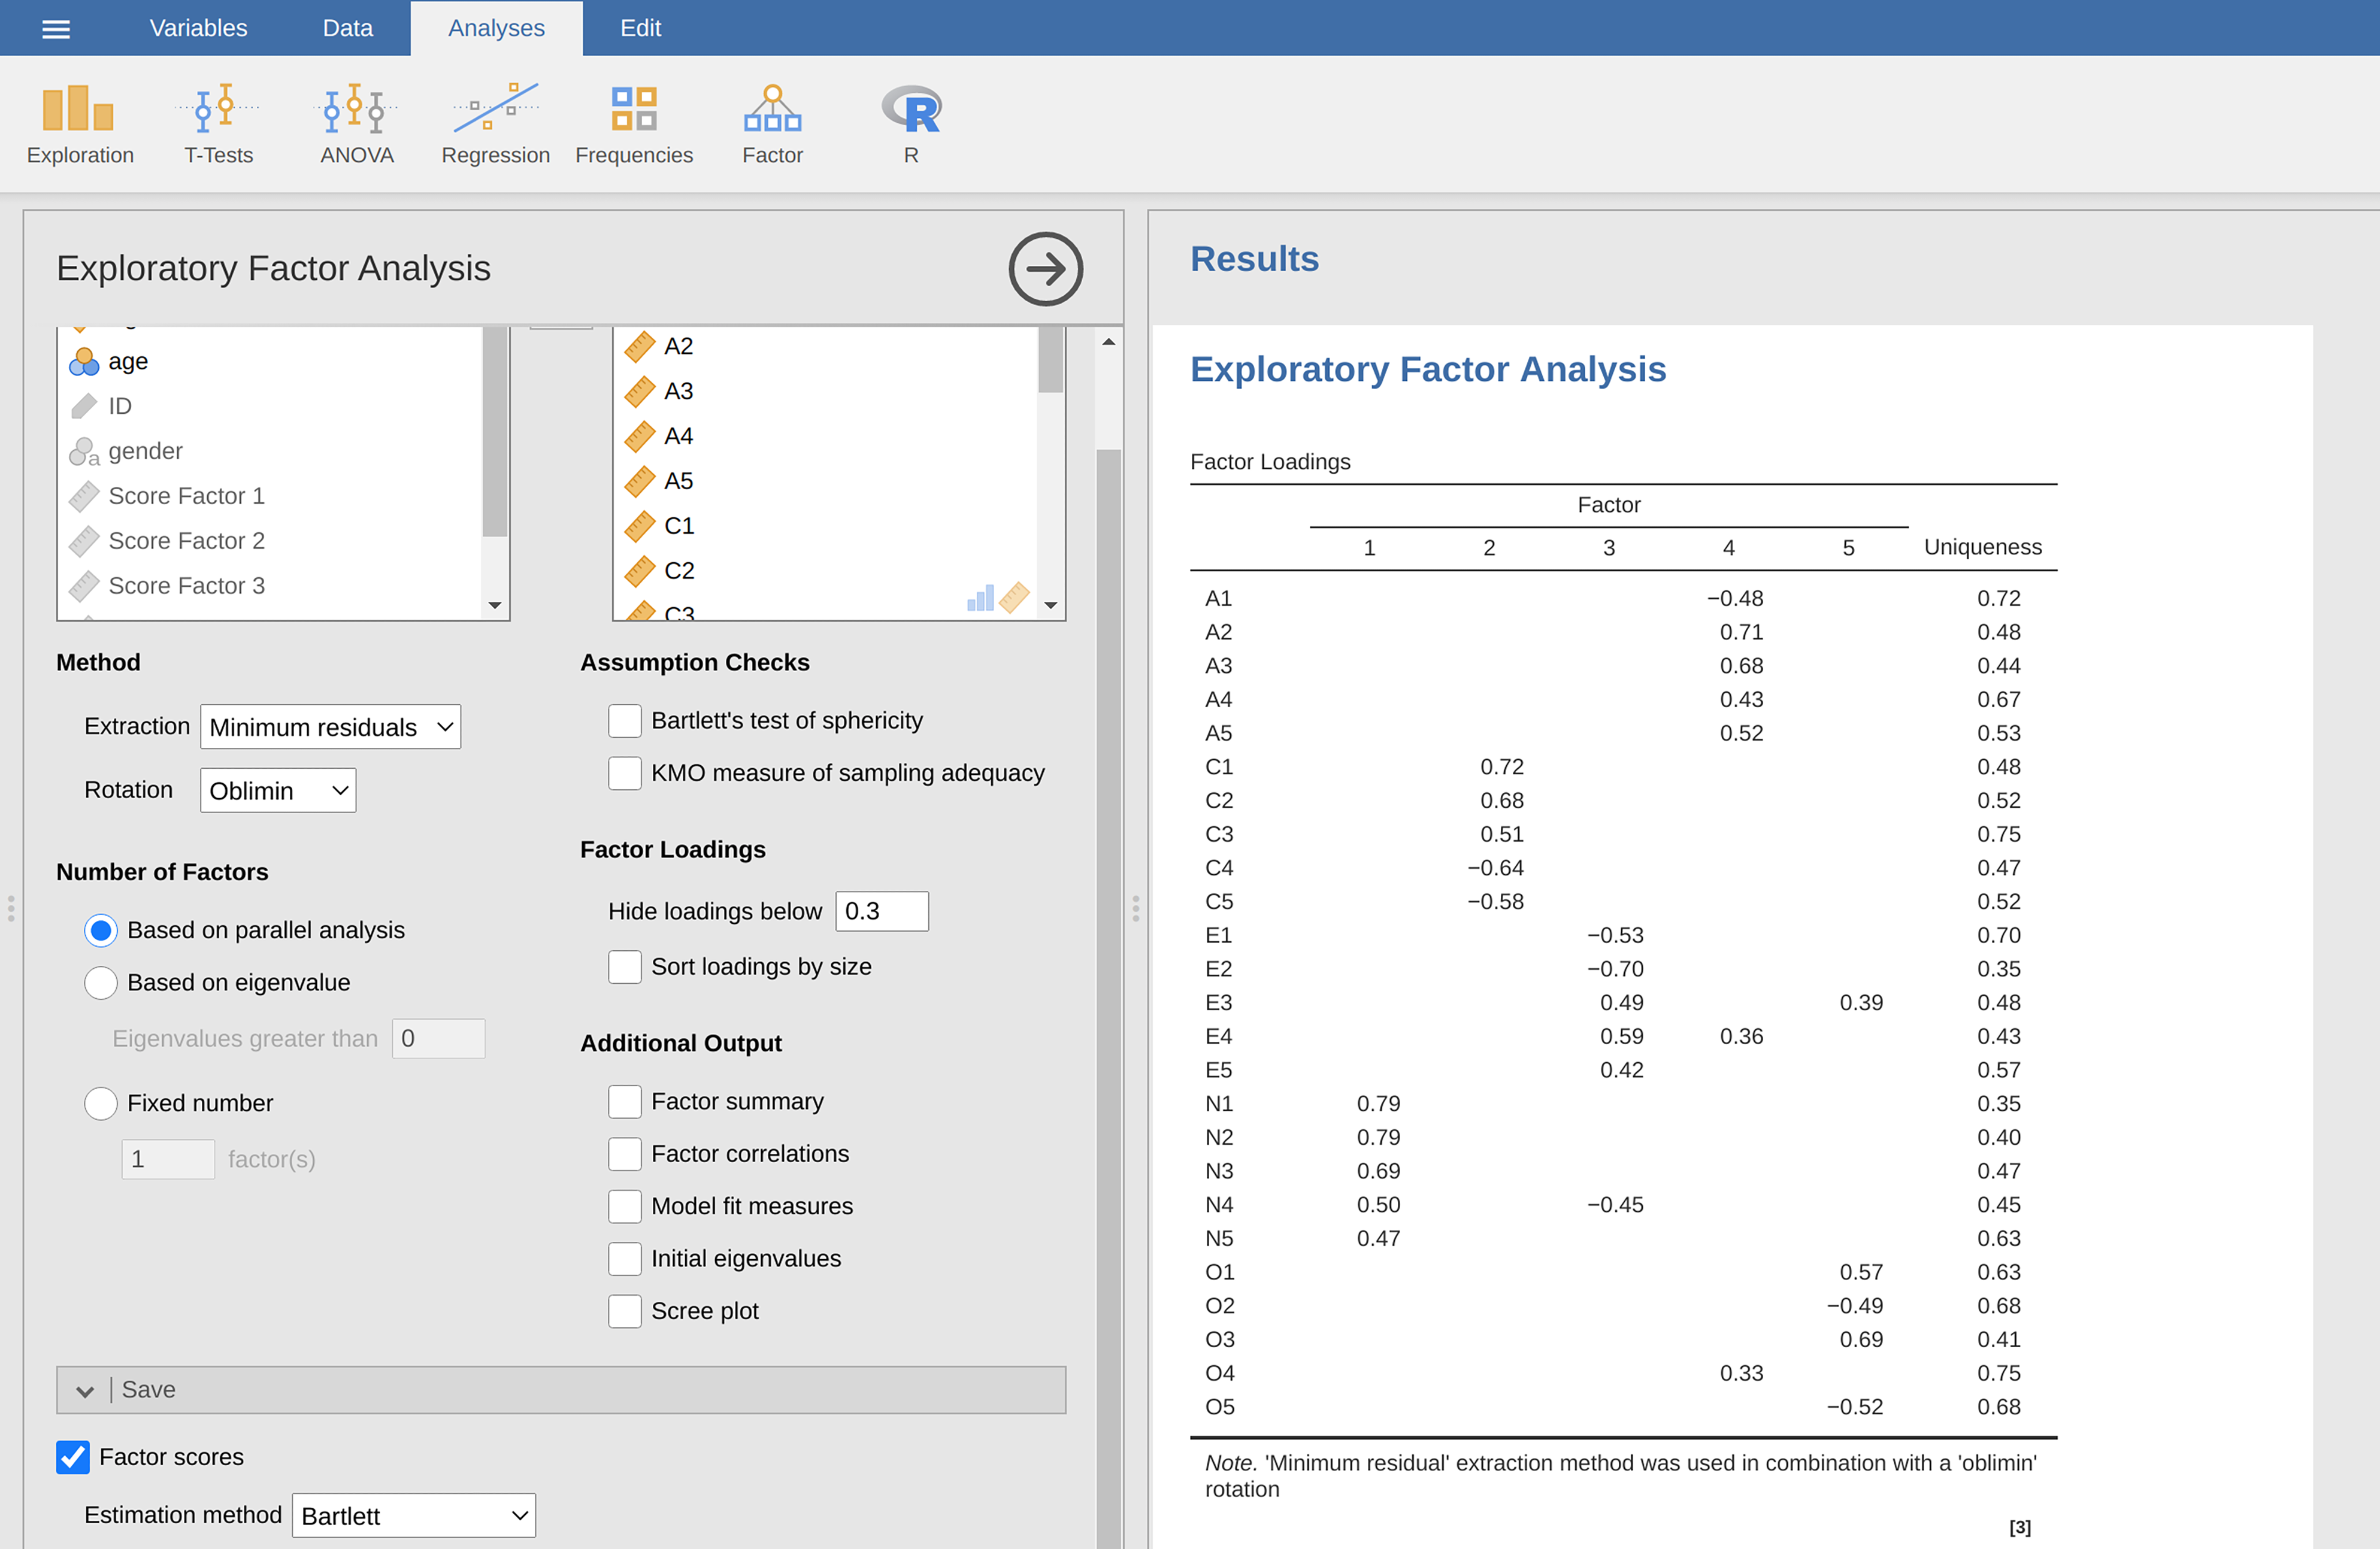
\includegraphics[width=1\textwidth,height=\textheight]{images/fig15-9.png} \hfill{}

\caption{\label{fig-fig15-9}Compute new scale score variable using the
jamovi Computed variable command}

\end{figure}

Another option is to create an \textbf{optimally-weighted} factor score
index. To do this, save the factor scores to the data set, using the
`Save' - `Factor scores' checkbox. Once you have done this you will see
that five new variables (columns) have been added to the data, one for
each factor extracted. See Figure~\ref{fig-fig15-10} and
Figure~\ref{fig-fig15-11}.

\begin{figure}

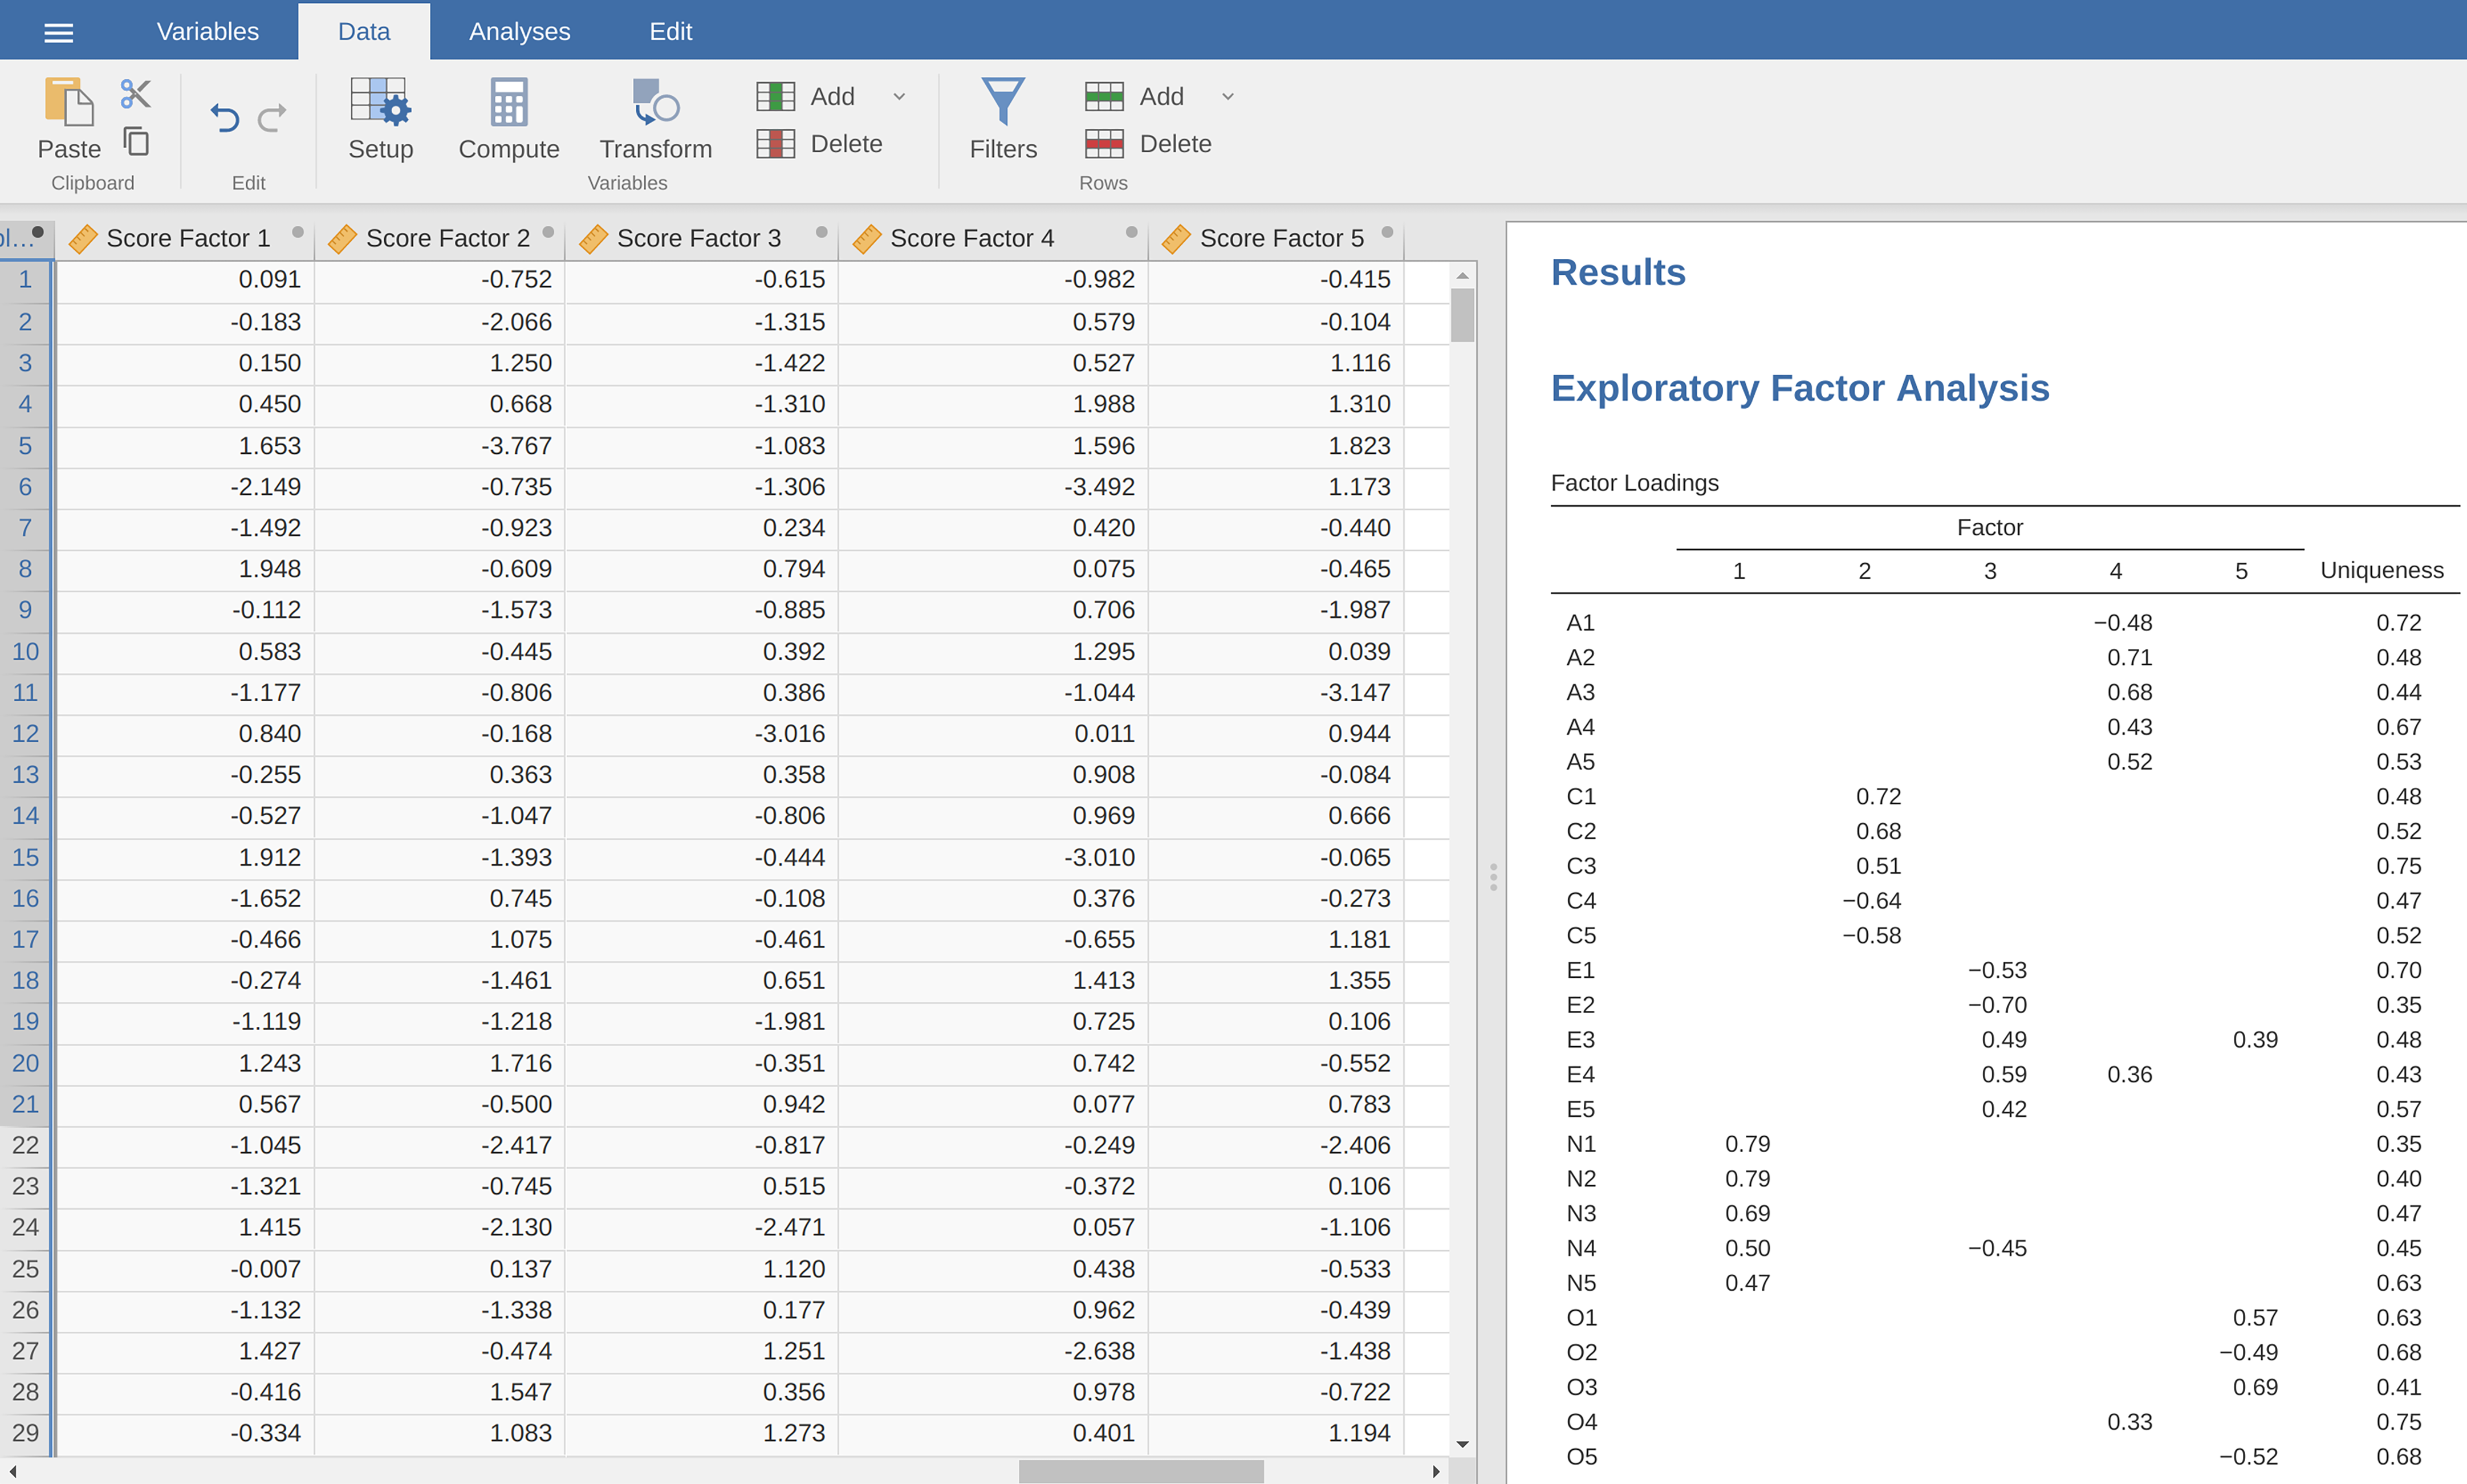
\includegraphics[width=1\textwidth,height=\textheight]{images/fig15-10.png} \hfill{}

\caption{\label{fig-fig15-10}jamovi option for factor scores for the
five factor solution, using the `Bartlett' optimal weighting method}

\end{figure}

\begin{figure}


\includegraphics[width=1\textwidth,height=\textheight]{images/fig15-11.png} \hfill{}

\caption{\label{fig-fig15-11}Data sheet view showing the five newly
created factor score variables}

\end{figure}

Now you can go ahead and undertake further analyses, using either the
mean score based factor scales (e.g.~as in Figure~\ref{fig-fig15-9}) or
using the optimally-weighted factor scores calculated by jamovi. Your
choice! For example, one thing you might like to do is see whether there
are any gender differences in each of our personality scales. We did
this for the Agreeableness score that we calculated using the mean score
approach, and although the \(t\)-test plot (Figure~\ref{fig-fig15-12})
showed that males were less agreeable than females, this was not a
significant difference (Mann-Whitney \(U = 5768\), \(p = .075\)).

\begin{figure}

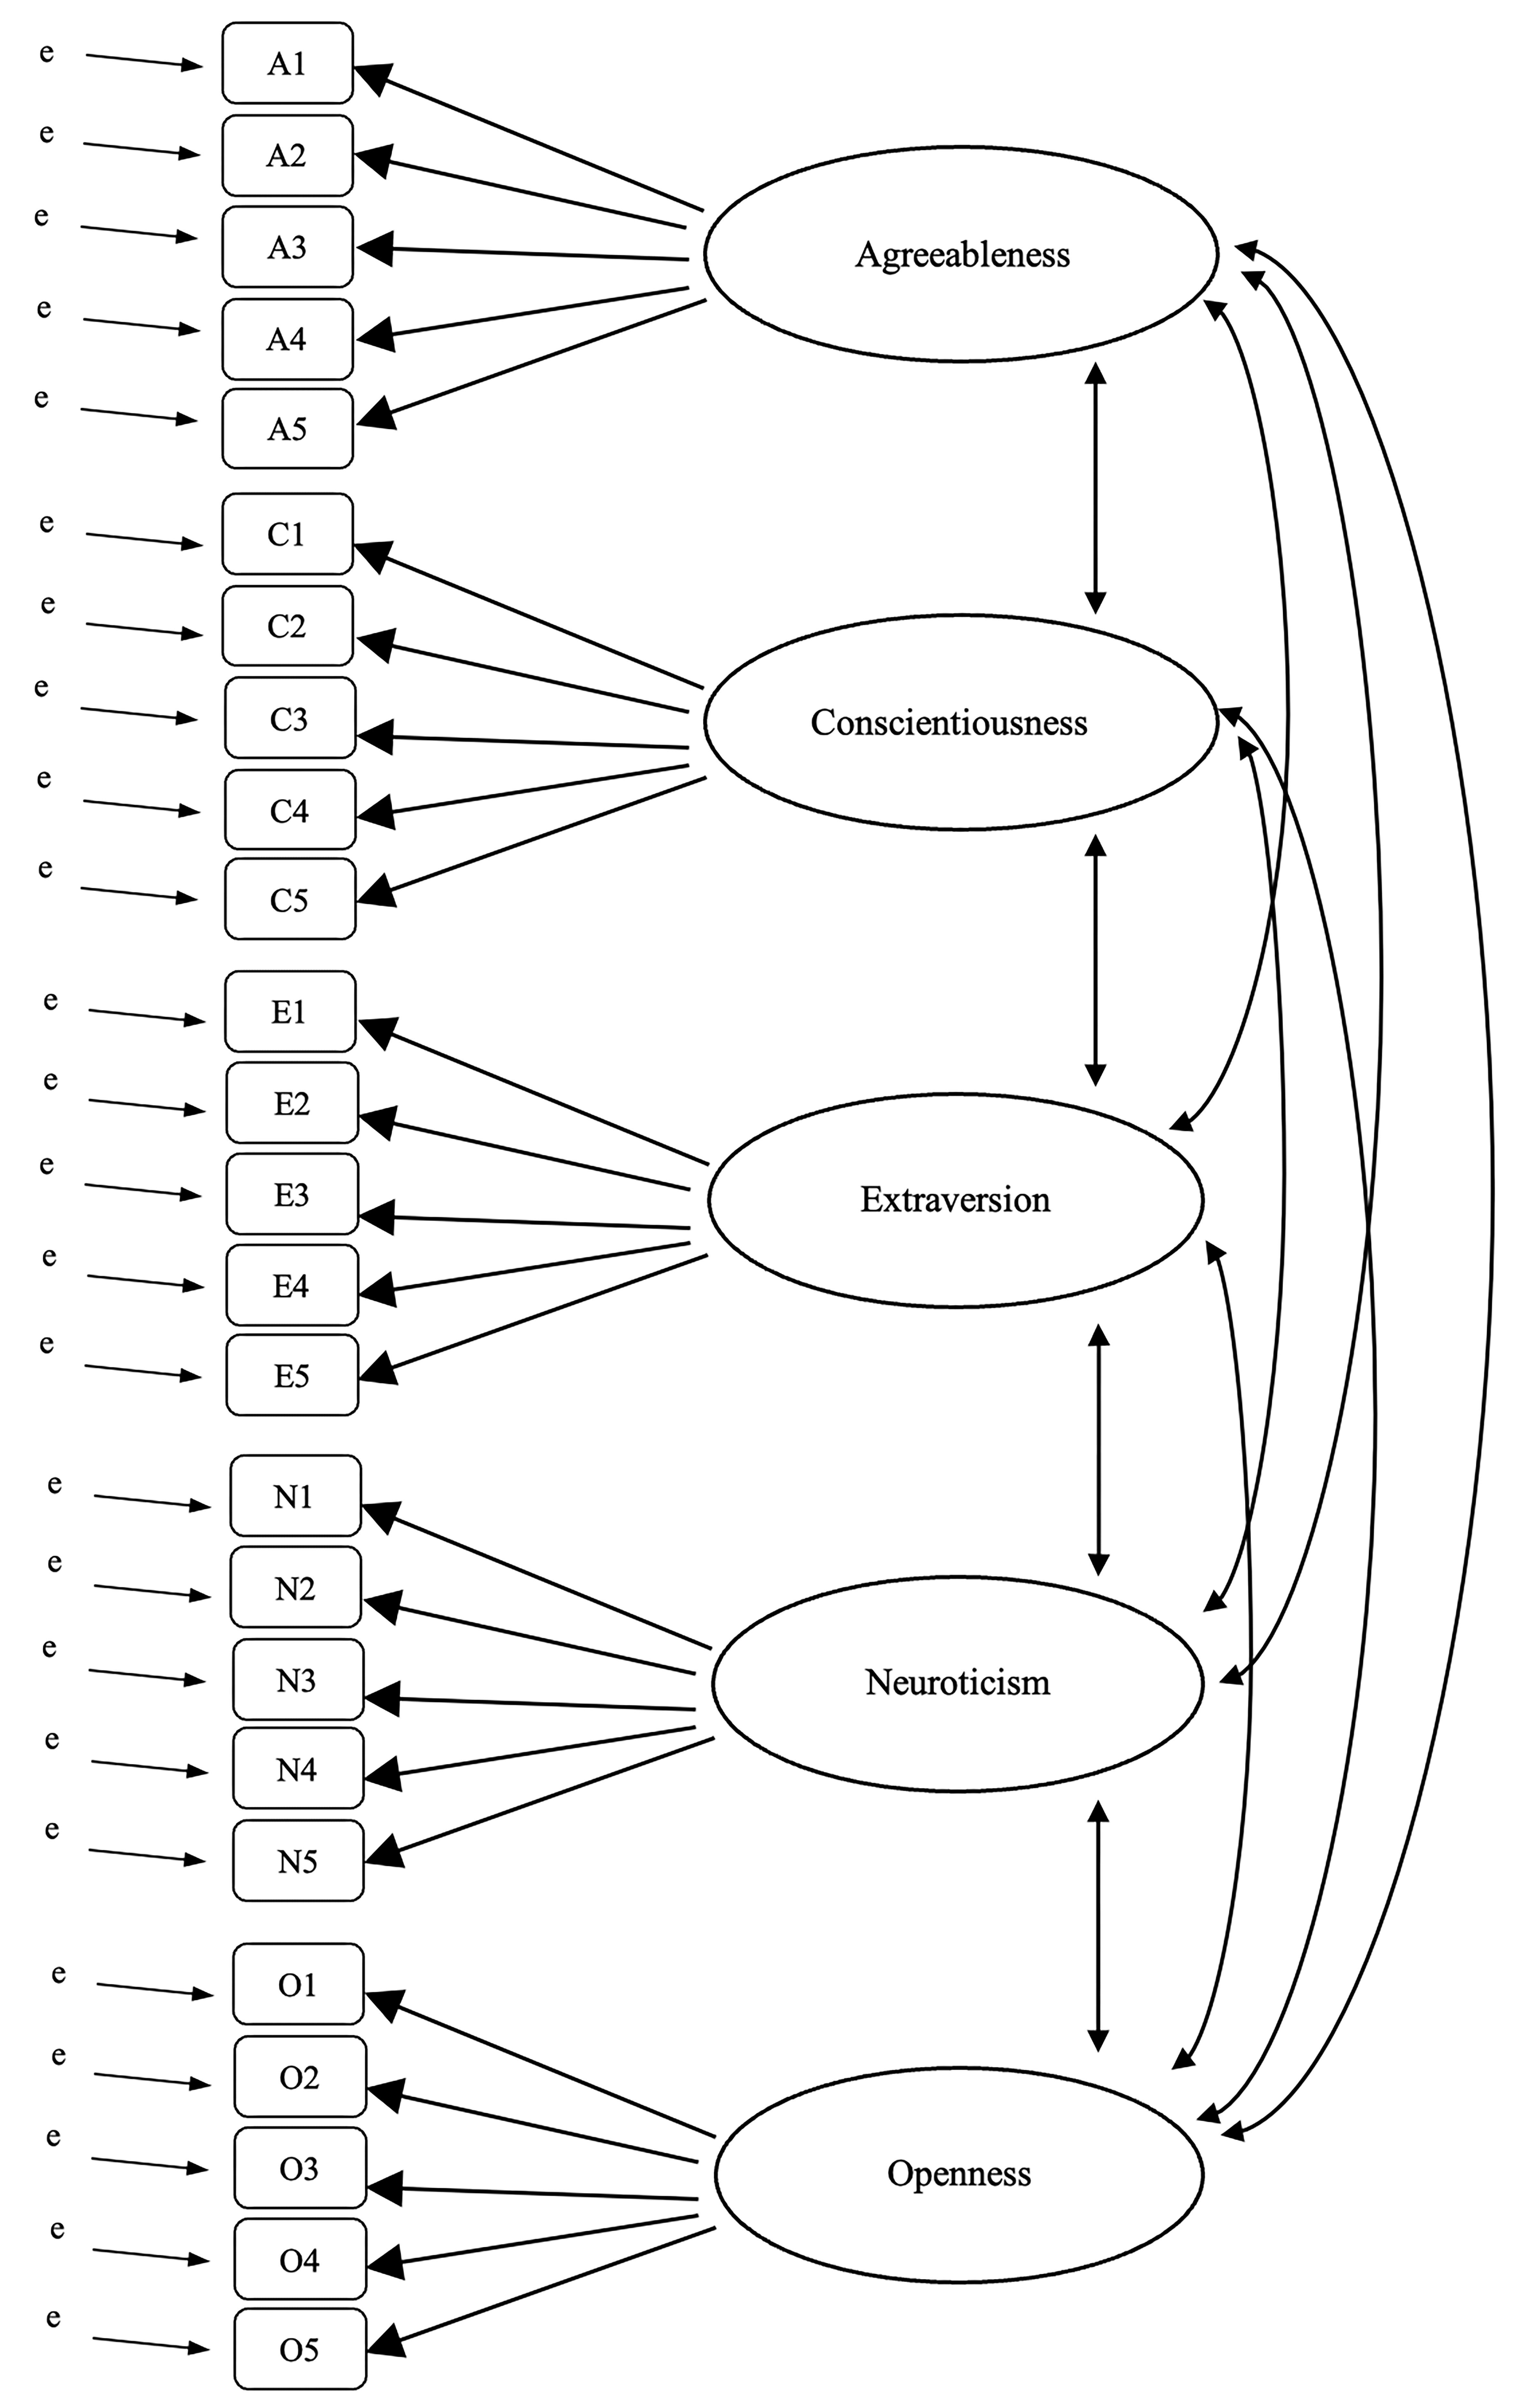
\includegraphics[width=1\textwidth,height=\textheight]{images/fig15-12.png} \hfill{}

\caption{\label{fig-fig15-12}Comparing differences in Agreeableness
factor-based scores between males and females}

\end{figure}

\hypertarget{writing-up-an-efa}{%
\subsection{Writing up an EFA}\label{writing-up-an-efa}}

Hopefully, so far we have given you some sense of EFA and how to
undertake EFA in jamovi. So, once you have completed your EFA, how do
you write it up? There is not a formal standard way to write up an EFA,
and examples tend to vary by discipline and researcher. That said, there
are some fairly standard pieces of information to include in your
write-up:

\begin{enumerate}
\def\labelenumi{\arabic{enumi}.}
\item
  What are the theoretical underpinnings for the area you are studying,
  and specifically for the constructs that you are interested in
  uncovering through EFA.
\item
  A description of the sample (e.g.~demographic information, sample
  size, sampling method).
\item
  A description of the type of data used (e.g., nominal, continuous) and
  descriptive statistics.
\item
  Describe how you went about testing the assumptions for EFA. Details
  regarding sphericity checks and measures of sampling adequacy should
  be reported.
\item
  Explain what FA extraction method (e.g.~`Minimum residuals' or
  `Maximum likelihood') was used.
\item
  Explain the criteria and process used for deciding how many factors
  were extracted in the final solution, and which items were selected.
  Clearly explain the rationale for key decisions during the EFA
  process.
\item
  Explain what rotation methods were attempted, the reasons why, and the
  results.
\item
  Final factor loadings should be reported in the results, in a table.
  This table should also report the uniqueness (or communality) for each
  variable (in the final column). Factor loadings should be reported
  with descriptive labels in addition to item numbers. Correlations
  between the factors should also be included, either at the bottom of
  this table, in a separate table.
\item
  Meaningful names for the extracted factors should be provided. You may
  like to use previously selected factor names, but on examining the
  actual items and factors you may think a different name is more
  appropriate
\end{enumerate}

\hypertarget{principal-component-analysis}{%
\section{Principal Component
Analysis}\label{principal-component-analysis}}

In the previous section we saw that EFA works to identify underlying
latent factors. And, as we saw, in one scenario the smaller number of
latent factors can be used in further statistical analysis using some
sort of combined factor scores.

In this way EFA is being used as a ``data reduction'' technique. Another
type of data reduction technique, sometimes seen as part of the EFA
family, is \textbf{principal component analysis (PCA)} . However, PCA
does not identify underlying latent factors. Instead it creates a linear
composite score from a larger set of measured variables.

PCA simply produces a mathematical transformation to the original data
with no assumptions about how the variables co-vary. The aim of PCA is
to calculate a few linear combinations (components) of the original
variables that can be used to summarize the observed data set without
losing much information. However, if identification of underlying
structure is a goal of the analysis, then EFA is to be preferred. And,
as we saw, EFA produces factor scores that can be used for data
reduction purposes just like principal component scores (Fabrigar et
al., 1999).

PCA has been popular in Psychology for a number of reasons, and
therefore it's worth mentioning, although nowadays EFA is just as easy
to do given the power of desktop computers and can be less susceptible
to bias than PCA, especially with a small number of factors and
variables. Much of the procedure is similar to EFA, so although there
are some conceptual differences, practically the steps are the same, and
with large samples and a sufficient number of factors and variables, the
results from PCA and EFA should be fairly similar.

To undertake PCA in jamovi, all you need to do is select `Factor' -
`Principal Component Analysis' from the main jamovi button bar to open
the PCA analysis window. Then you can follow the same steps from
\protect\hyperlink{efa-in-jamovi}{EFA in jamovi} above.

\hypertarget{confirmatory-factor-analysis}{%
\section{Confirmatory Factor
Analysis}\label{confirmatory-factor-analysis}}

So, our attempt to identify underlying latent factors using EFA with
carefully selected questions from the personality item pool seemed to be
pretty successful. The next step in our quest to develop a useful
measure of personality is to check the latent factors we identified in
the original EFA with a different sample. We want to see if the factors
hold up, if we can confirm their existence with different data. This is
a more rigorous check, as we will see. And it's called
\textbf{Confirmatory Factor Analysis (CFA)} as we will, unsurprisingly,
be seeking to confirm a pre-specified latent factor
structure.\footnote{As an aside, given that we had a pretty firm idea
  from our initial ``putative'' factors, we could just have gone
  straight to CFA and skipped the EFA step. Whether you use EFA and then
  go on to CFA, or go straight to CFA, is a matter of judgement and how
  confident you are initially that you have the model about right (in
  terms of number of factors and variables). Earlier on in the
  development of scales, or the identification of underlying latent
  constructs, researchers tend to use EFA. Later on, as they get closer
  to a final scale, or if they want to check an established scale in a
  new sample, then CFA is a good option.}

In CFA, instead of doing an analysis where we see how the data goes
together in an exploratory sense, we instead impose a structure, like in
Figure~\ref{fig-fig15-13}, on the data and see how well the data fits
our pre-specified structure. In this sense, we are undertaking a
confirmatory analysis, to see how well a pre-specified \textbf{model} is
confirmed by the observed data.

A straightforward confirmatory factor analysis (CFA) of the personality
items would therefore specify five latent factors as shown in
Figure~\ref{fig-fig15-13}, each measured by five observed variables.
Each variable is a measure of an underlying latent factor. For example,
A1 is predicted by the underlying latent factor Agreeableness. And
because A1 is not a perfect measure of the Agreeableness factor, there
is an error term, \(e\), associated with it. In other words, \(e\)
represents the variance in A1 that is not accounted for by the
Agreeableness factor. This is sometimes called \textbf{measurement
error}.

\begin{figure}

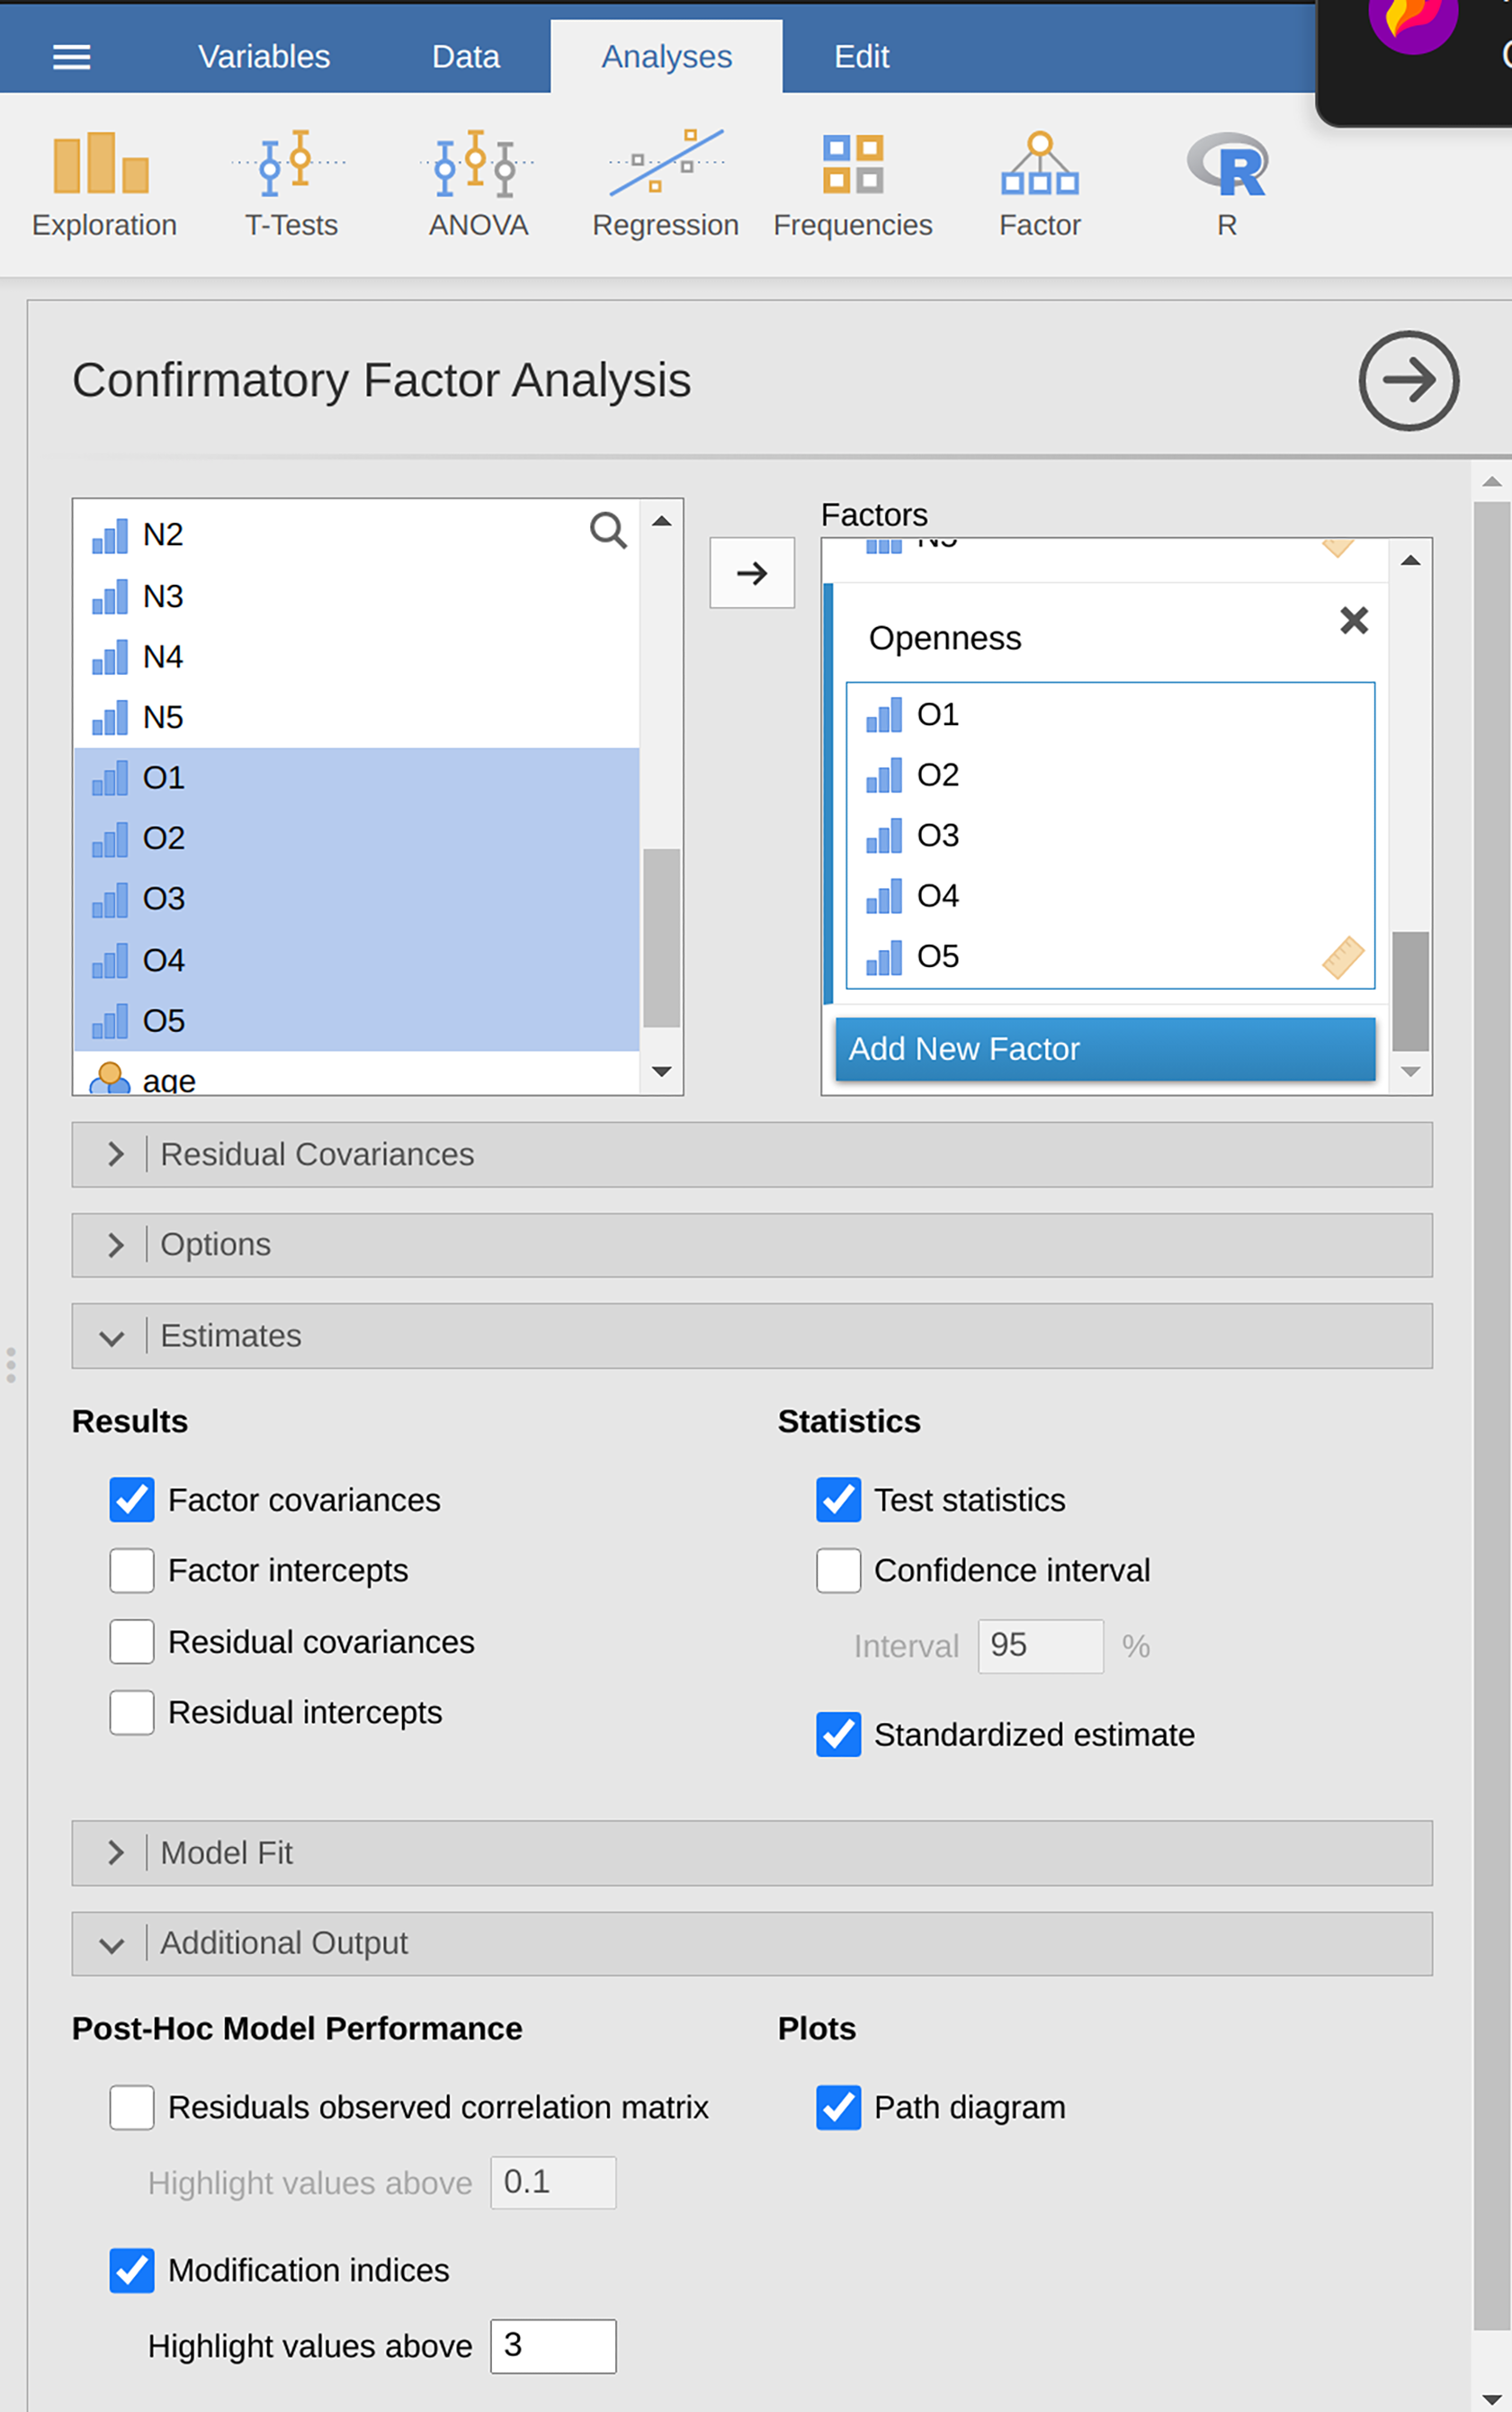
\includegraphics[width=1\textwidth,height=\textheight]{images/fig15-13.png} \hfill{}

\caption{\label{fig-fig15-13}Initial pre-specification of latent factor
structure for the five factor personality scales, for use in CFA}

\end{figure}

The next step is to consider whether the latent factors should be
allowed to correlate in our model. As mentioned earlier, in the
psychological and behavioural sciences constructs are often related to
each other, and we also think that some of our personality factors may
be correlated with each other. So, in our model, we should allow these
latent factors to co-vary, as shown by the double-headed arrows in
Figure~\ref{fig-fig15-13}.

At the same time, we should consider whether there is any good,
systematic, reason for some of the error terms to be correlated with
each other. One reason for this might be that there is a shared
methodological feature for particular sub-sets of the observed variables
such that the observed variables might be correlated for methodological
rather than substantive latent factor reasons. We'll return to this
possibility in a later section but, for now, there are no clear reasons
that we can see that would justify correlating some of the error terms
with each other

Without any correlated error terms, the model we are testing to see how
well it fits with our observed data is just as specified in
Figure~\ref{fig-fig15-13}. Only parameters that are included in the
model are expected to be found in the data, so in CFA all other possible
parameters (coefficients) are set to zero. So, if these other parameters
are not zero (for example there may be a substantial loading from A1
onto the latent factor Extraversion in the observed data, but not in our
model) then we may find a poor fit between our model and the observed
data.

Right, let's take a look at how we set this CFA analysis up in jamovi.

\hypertarget{cfa-in-jamovi}{%
\subsection{CFA in jamovi}\label{cfa-in-jamovi}}

Open up the \emph{bfi\_sample2.csv} file, check that the 25 variables
are coded as ordinal (or continuous; it won't make any difference for
this analysis). To perform CFA in jamovi:

\begin{itemize}
\item
  Select Factor - Confirmatory Factor Analysis from the main jamovi
  button bar to open the CFA analysis window
  (Figure~\ref{fig-fig15-14}).
\item
  Select the 5 A variables and transfer them into the `Factors' box and
  give then the label ``Agreeableness''.
\item
  Create a new Factor in the `Factors' box and label it
  ``Conscientiousness''. Select the 5 C variables and transfer them into
  the `Factors' box under the ``Conscientiousness'' label.
\item
  Create another new Factor in the `Factors' box and label it
  ``Extraversion''. Select the 5 E variables and transfer them into the
  `Factors' box under the ``Extraversion'' label.
\item
  Create another new Factor in the `Factors' box and label it
  ``Neuroticism''. Select the 5 ``N'' variables and transfer them into
  the `Factors' box under the ``Neuroticism'' label.
\item
  Create another new Factor in the `Factors' box and label it
  ``Openness''. Select the 5 O variables and transfer them into the
  `Factors' box under the ``Openness'' label.
\item
  Check other appropriate options, the defaults are ok for this initial
  work through, though you might want to check the ``Path diagram''
  option under `Plots' to see jamovi produce a (fairly) similar diagram
  to our Figure~\ref{fig-fig15-13}.
\end{itemize}

\begin{figure}

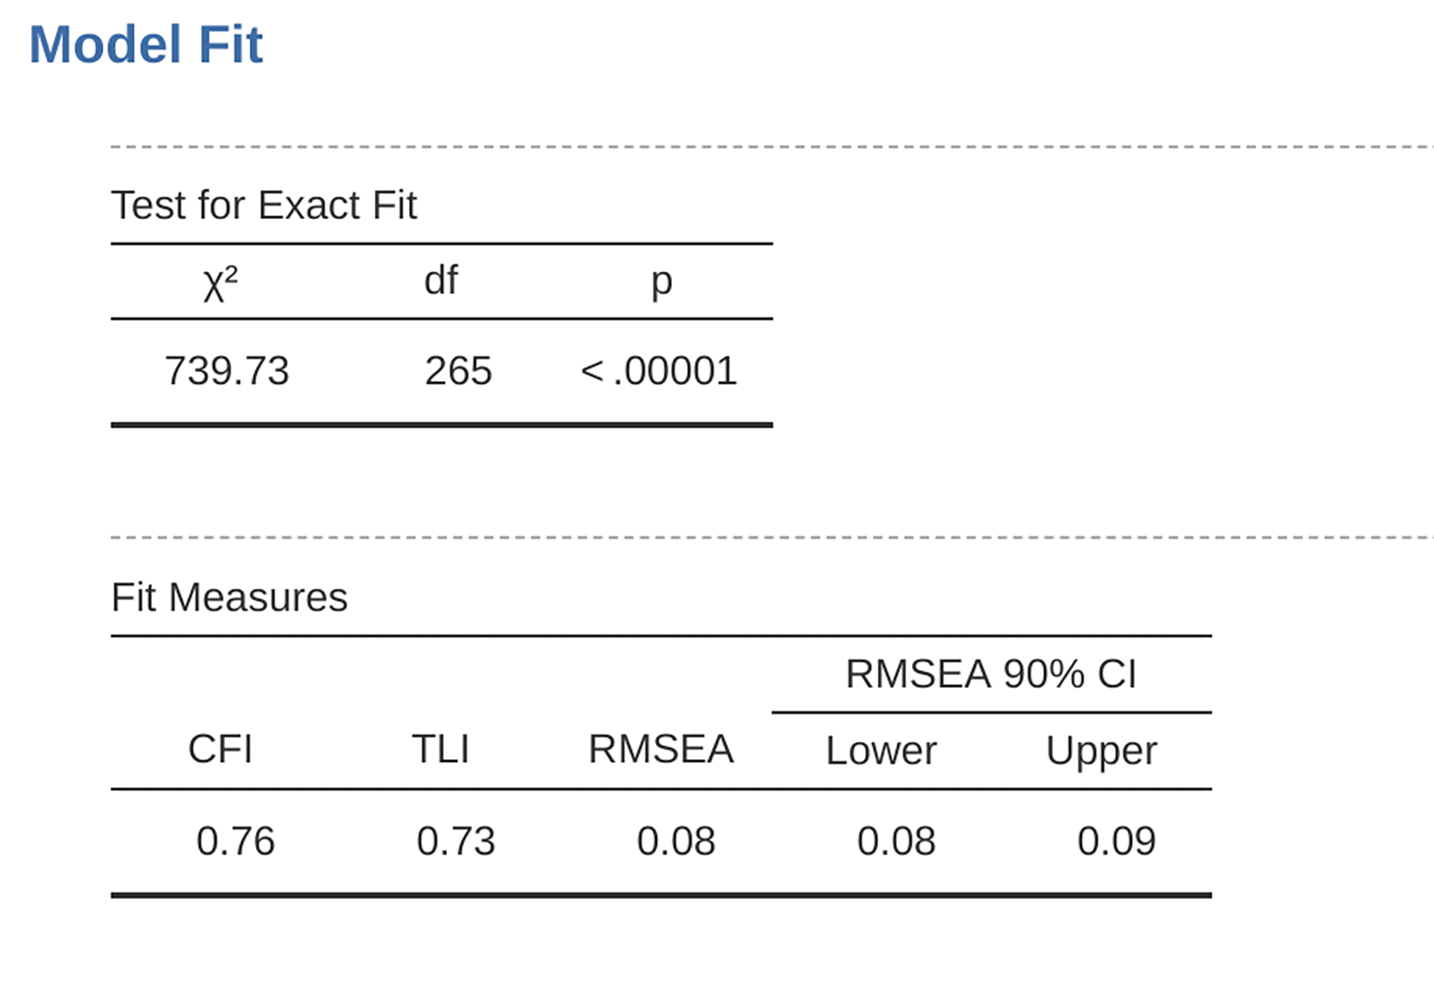
\includegraphics[width=1\textwidth,height=\textheight]{images/fig15-14.png} \hfill{}

\caption{\label{fig-fig15-14}The jamovi CFA analysis window}

\end{figure}

Once we have set up the analysis we can turn our attention to the jamovi
results window and see what's what. The first thing to look at is
\textbf{model fit} (Figure~\ref{fig-fig15-15}) as this tells us how good
a fit our model is to the observed data. NB in our model only the
pre-specified covariances are estimated, including the factor
correlations by default. Everything else is set to zero.

\begin{figure}

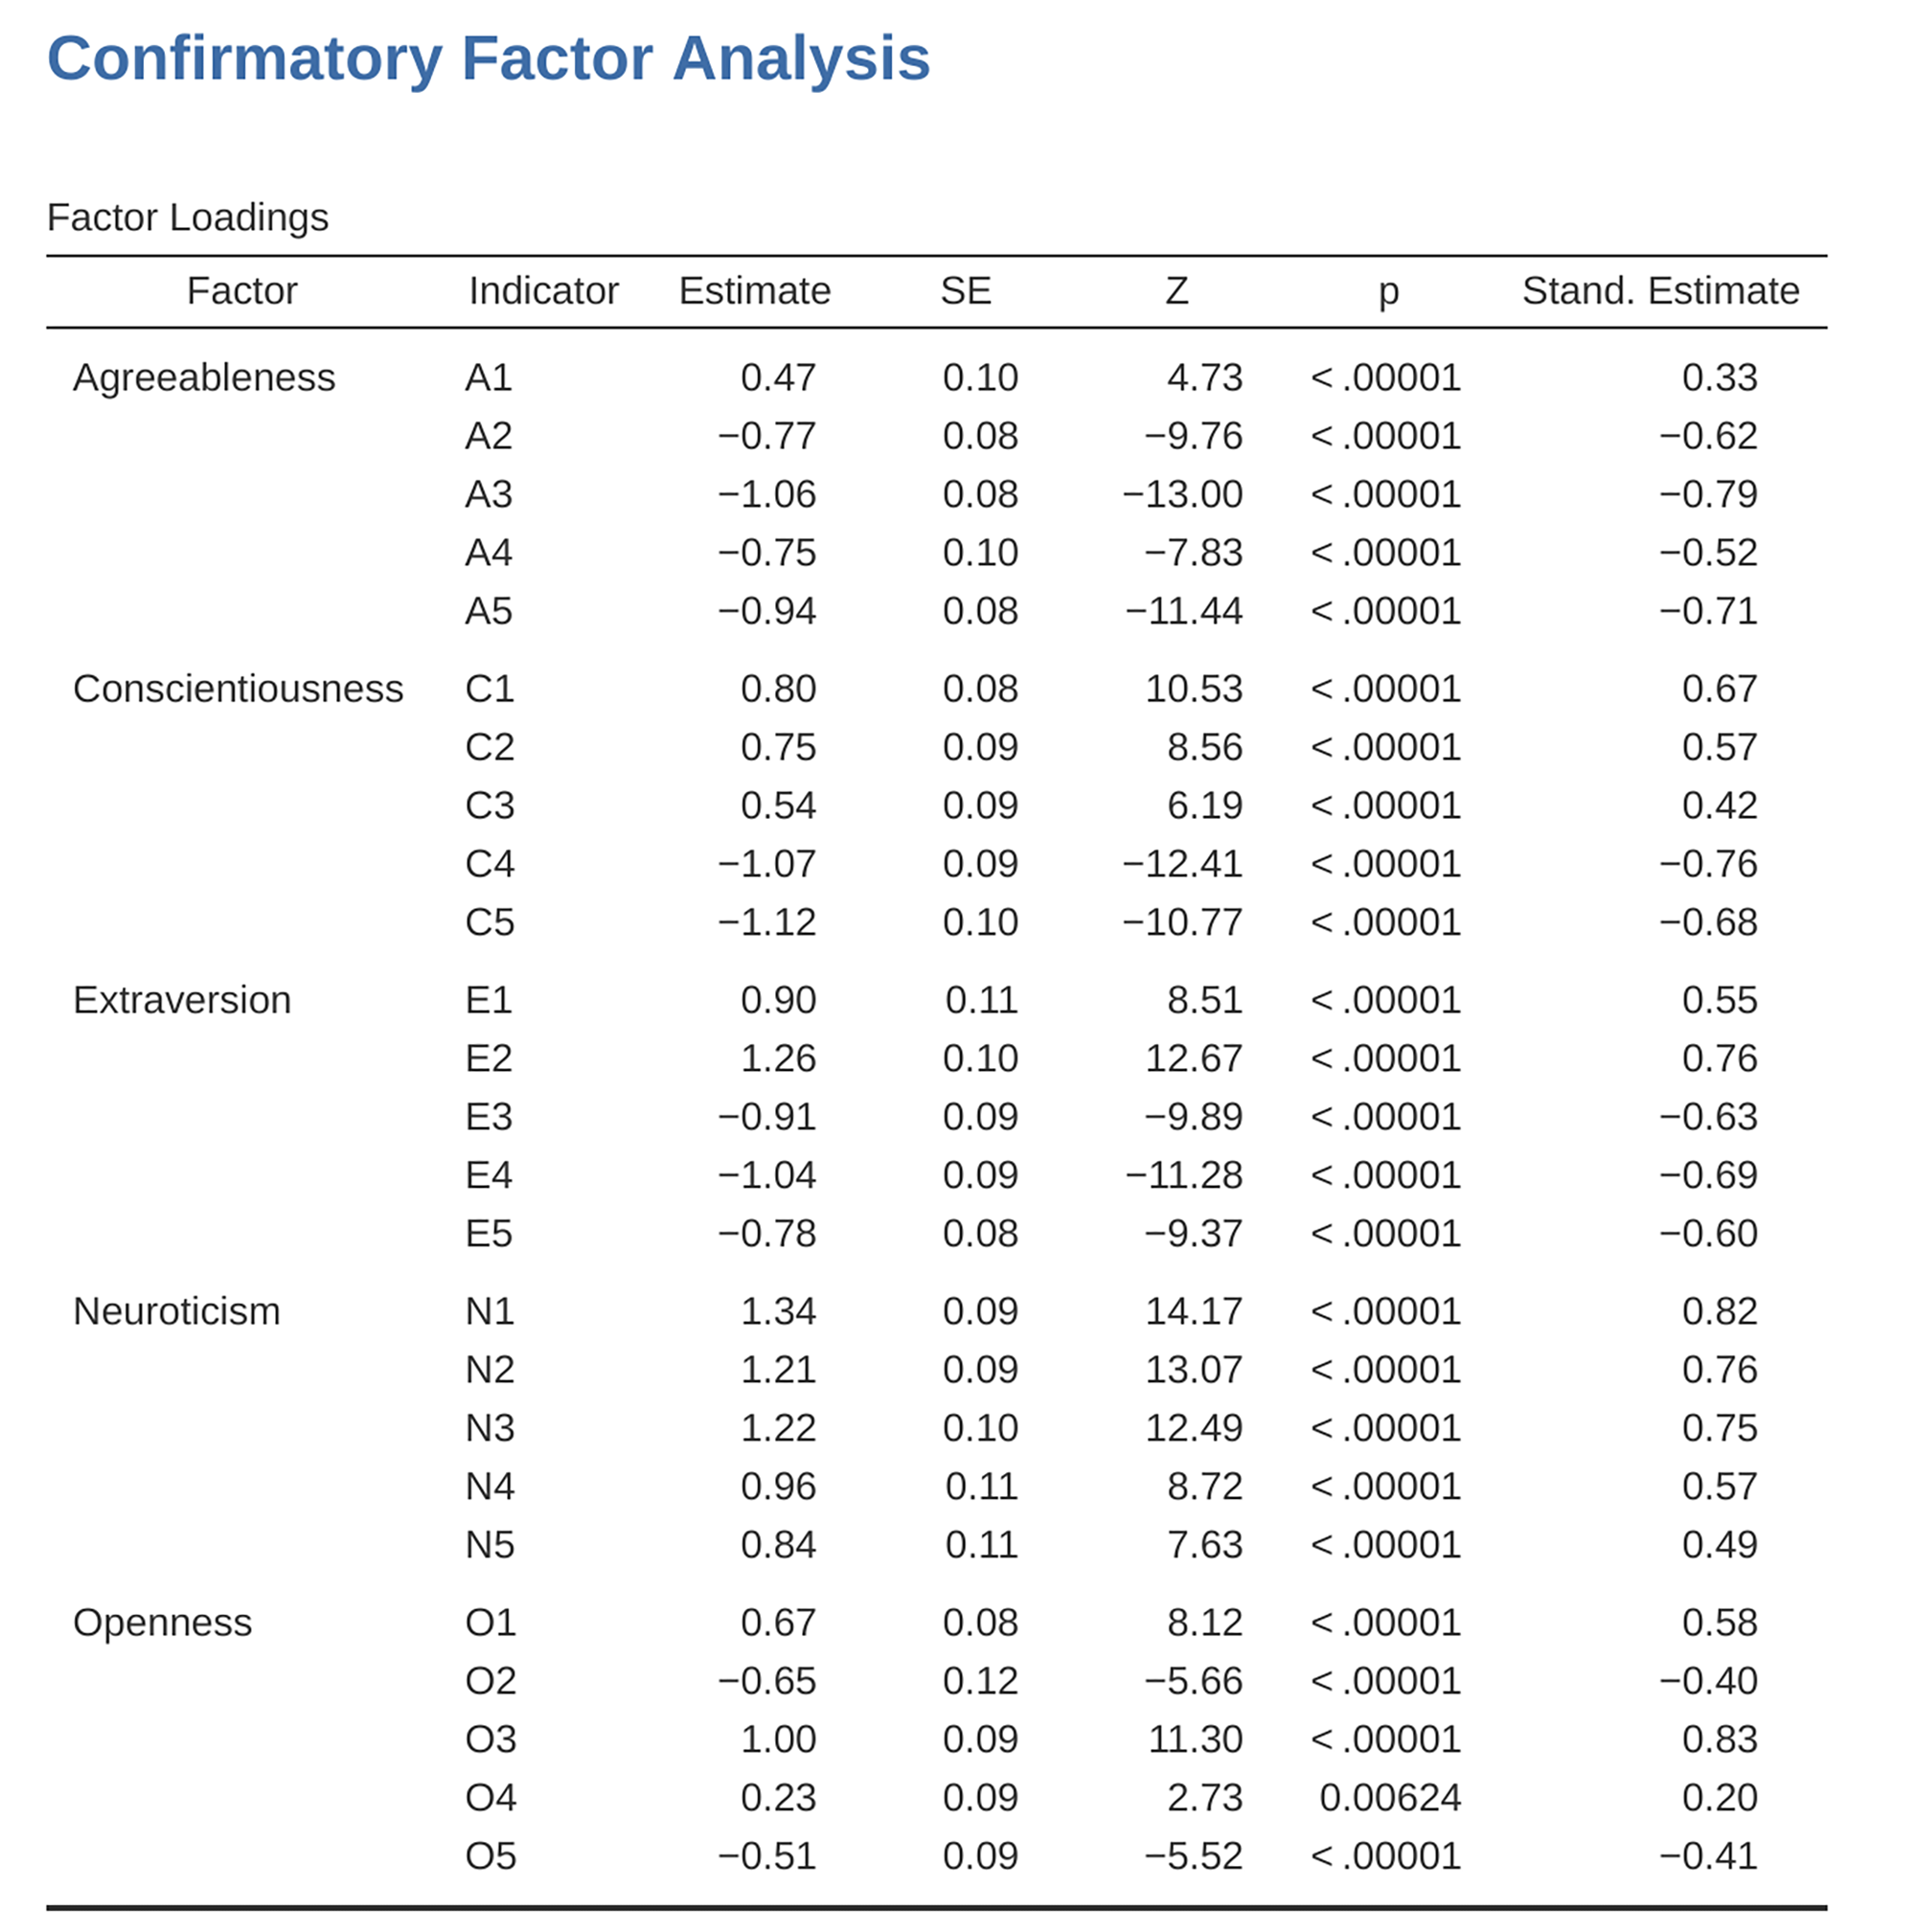
\includegraphics[width=1\textwidth,height=\textheight]{images/fig15-15.png} \hfill{}

\caption{\label{fig-fig15-15}The jamovi CFA Model Fit results for our
CFA model}

\end{figure}

There are several ways of assessing model fit. The first is a chi-square
statistic that, if small, indicates that the model is a good fit to the
data. However, the chi-squared statistic used for assessing model fit is
pretty sensitive to sample size, meaning that with a large sample a good
enough fit between the model and the data almost always produces a large
and significant (p \textless{} .05) chi-square value.

So, we need some other ways of assessing model fit. In jamovi several
are provided by default. These are the Comparative Fit Index (CFI), the
Tucker Lewis Index (TLI) and the Root Mean Square Error of Approximation
(RMSEA) together with the 90\% confidence interval for the RMSEA. Some
useful rules of thumb are that a satisfactory fit is indicated by CFI
\textgreater{} 0.9, TLI \textgreater{} 0.9, and RMSEA of about 0.05 to
0.08. A good fit is CFI \textgreater{} 0.95, TLI \textgreater{} 0.95,
and RMSEA and upper CI for RMSEA \textless{} 0.05.

So, looking at Figure~\ref{fig-fig15-15} we can see that the chi-square
value is large and highly significant. Our sample size is not too large,
so this possibly indicates a poor fit. The CFI is \(0.762\) and the TLI
is 0.731, indicating poor fit between the model and the data. The RMSEA
is \(0.085\) with a \(90\%\) confidence interval from \(0.077\) to
\(0.092\), again this does not indicate a good fit.

Pretty disappointing, huh? But perhaps not too surprising given that in
the earlier EFA, when we ran with a similar data set (see
\protect\hyperlink{exploratory-factor-analysis}{Exploratory Factor
Analysis} section), only around half of the variance in the data was
accounted for by the five factor model.

Let's go on to look at the factor loadings and the factor covariance
estimates, shown in Figure~\ref{fig-fig15-16} and
Figure~\ref{fig-fig15-17}. The Z-statistic and \(p\)-value for each of
these parameters indicates they make a reasonable contribution to the
model (i.e.~they are not zero) so there doesn't appear to be any reason
to remove any of the specified variable-factor paths, or factor-factor
correlations from the model. Often the standardized estimates are easier
to interpret, and these can be specified under the `Estimates' option.
These tables can usefully be incorporated into a written report or
scientific article.

\begin{figure}

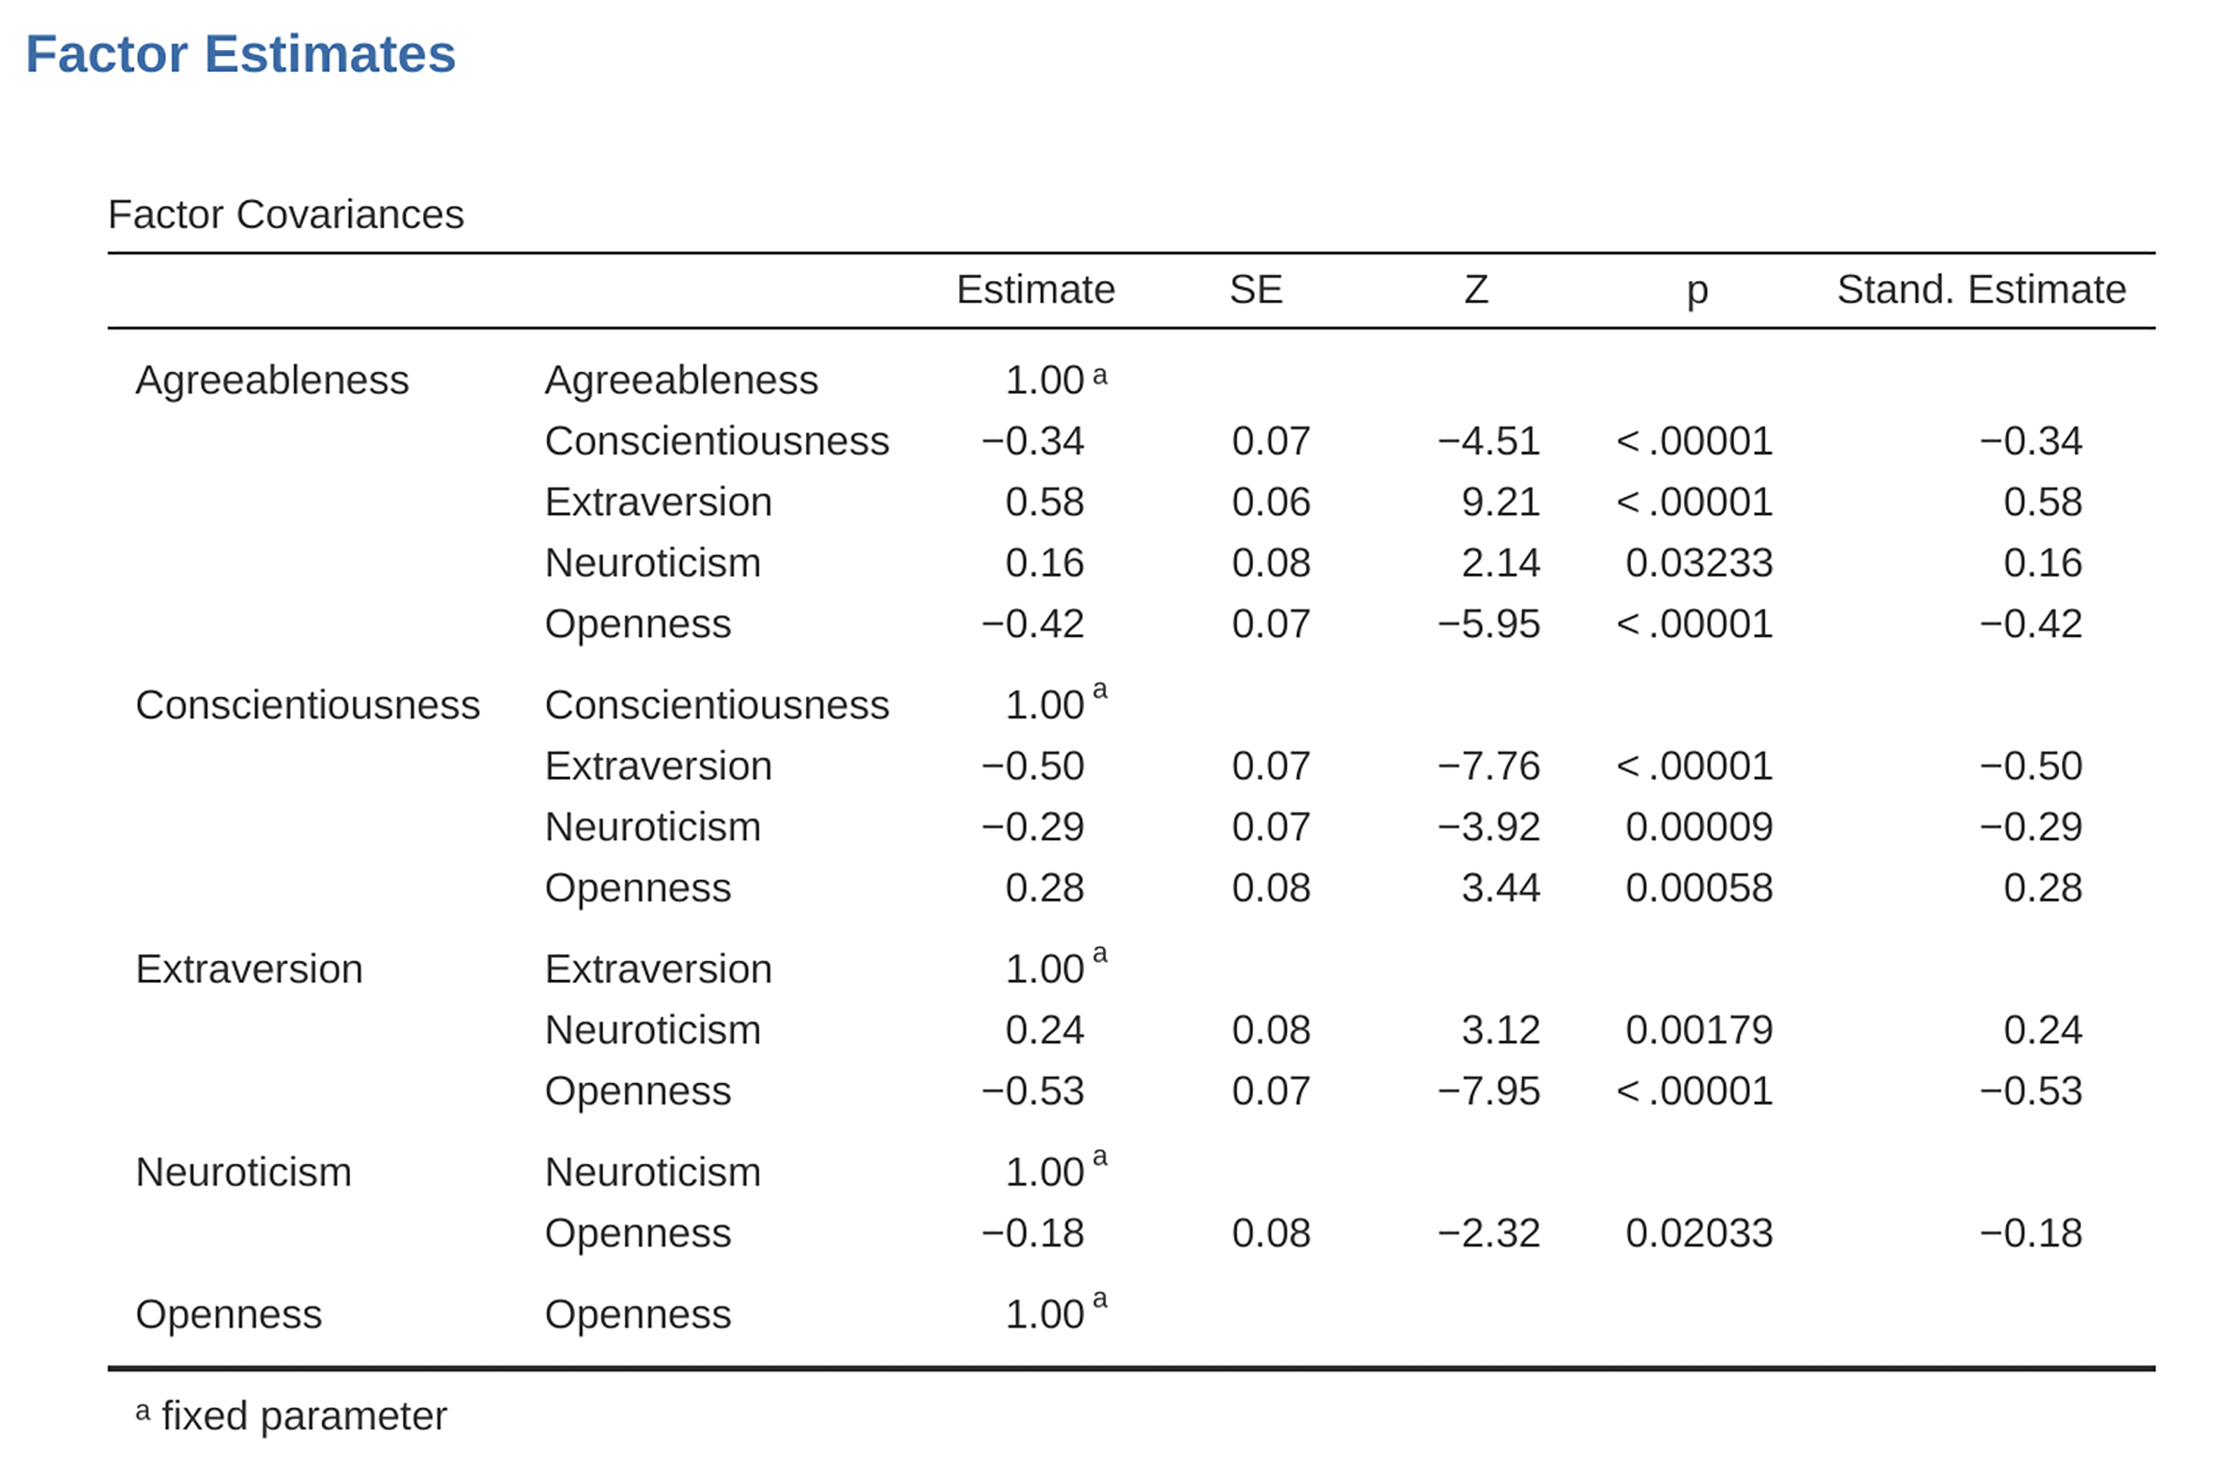
\includegraphics[width=1\textwidth,height=\textheight]{images/fig15-16.png} \hfill{}

\caption{\label{fig-fig15-16}The jamovi CFA Factor Loadings table for
our CFA model}

\end{figure}

\begin{figure}

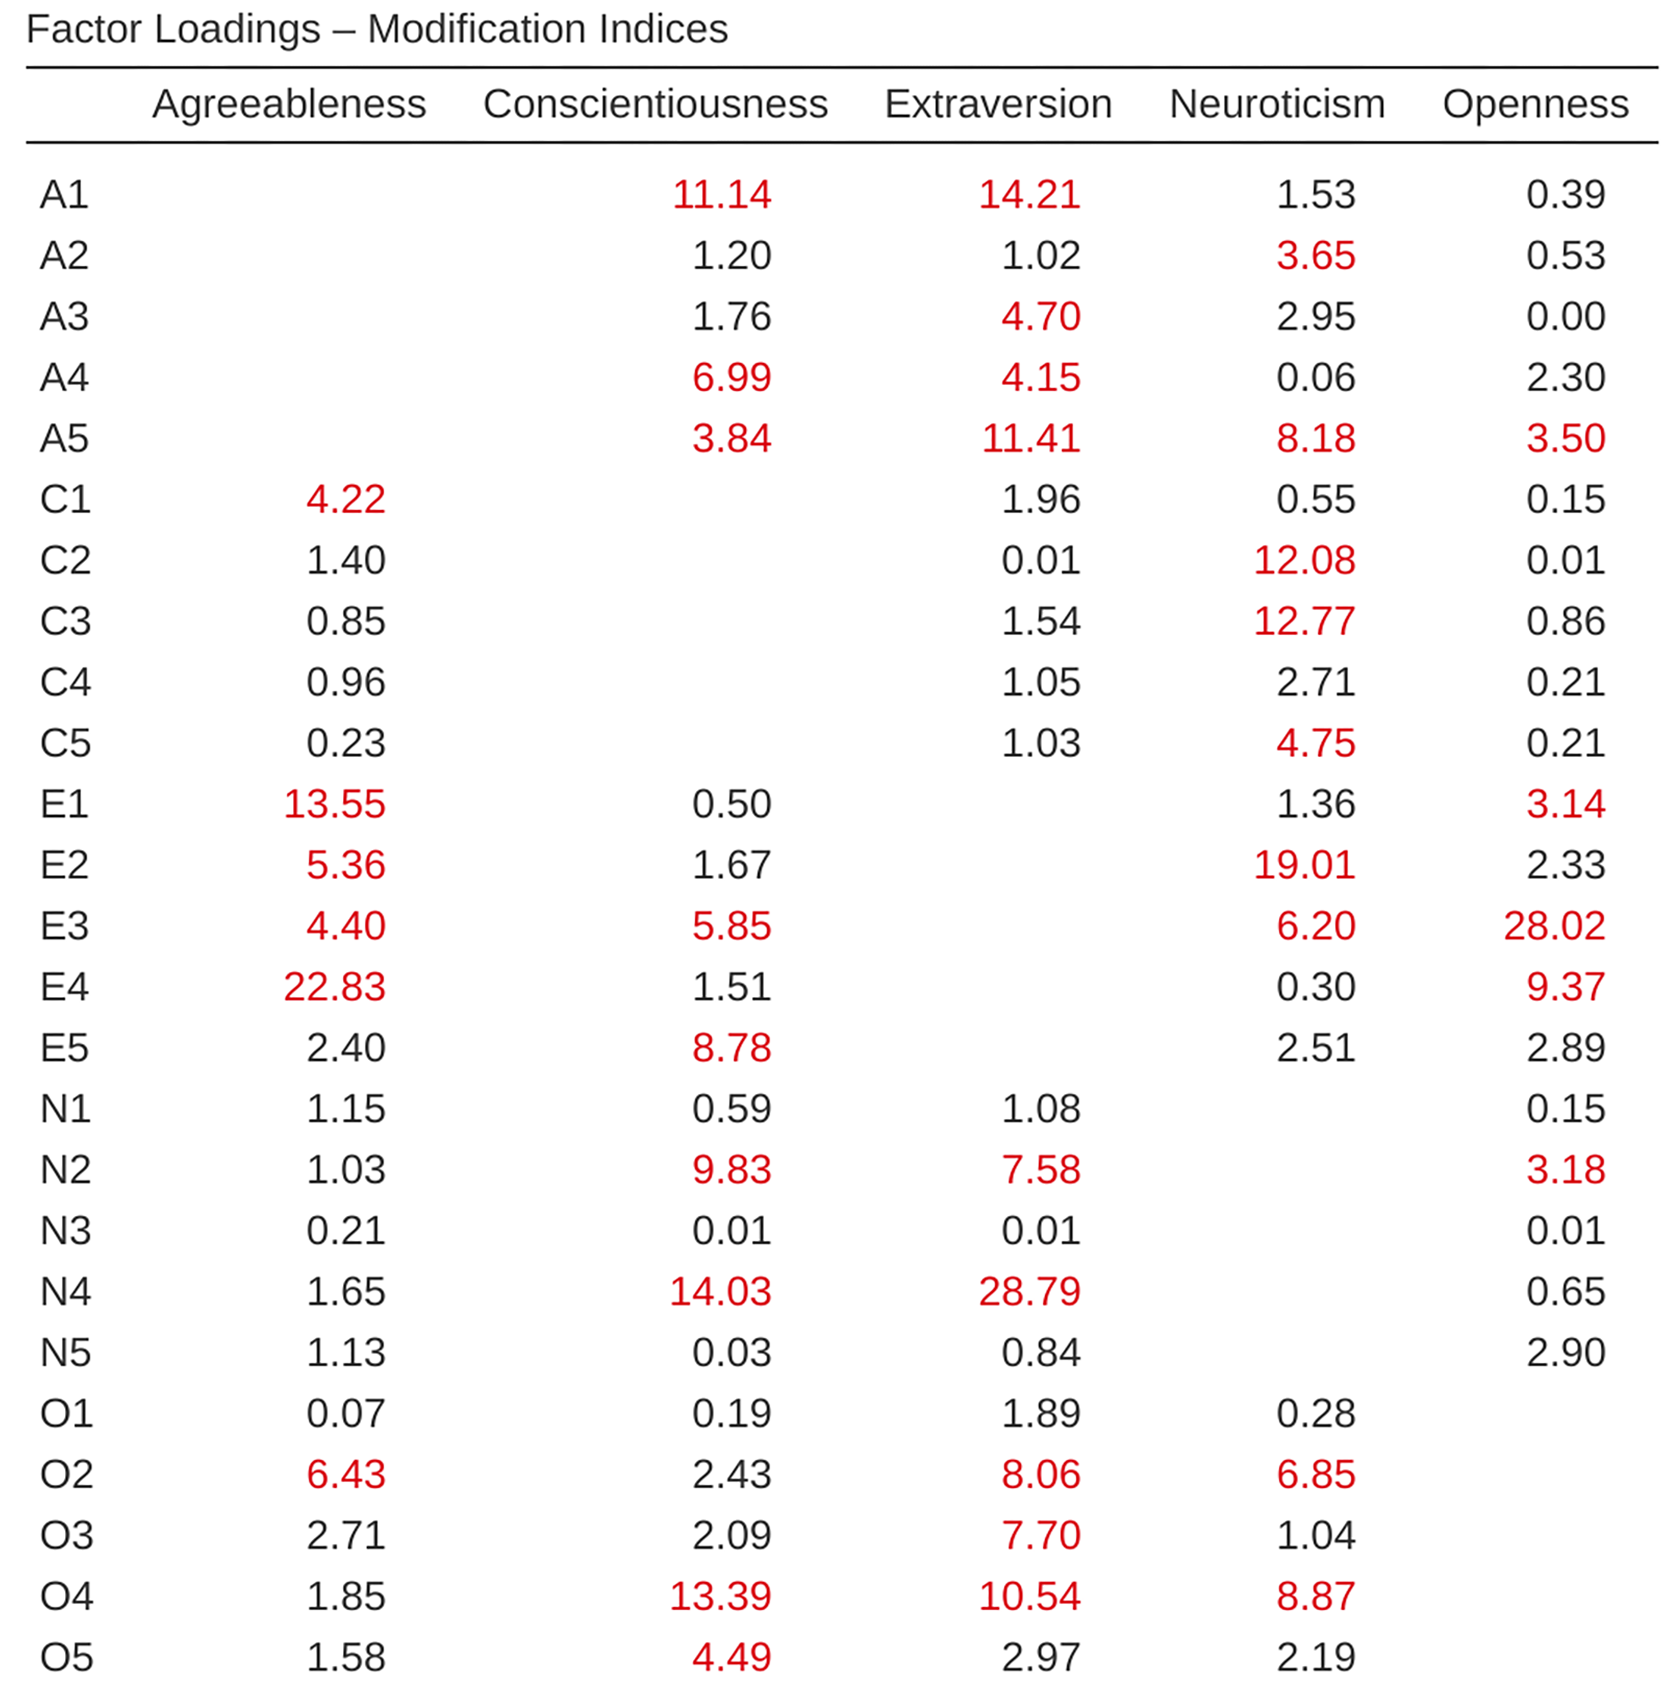
\includegraphics[width=1\textwidth,height=\textheight]{images/fig15-17.png} \hfill{}

\caption{\label{fig-fig15-17}The jamovi CFA Factor Covariances table for
our CFA model}

\end{figure}

How could we improve the model? One option is to go back a few stages
and think again about the items / measures we are using and how they
might be improved or changed. Another option is to make some post hoc
tweaks to the model to improve the fit. One way of doing this is to use
``modification indices'' (Figure~\ref{fig-fig15-18}), specified as an
`Additional output' option in jamovi.

\begin{figure}

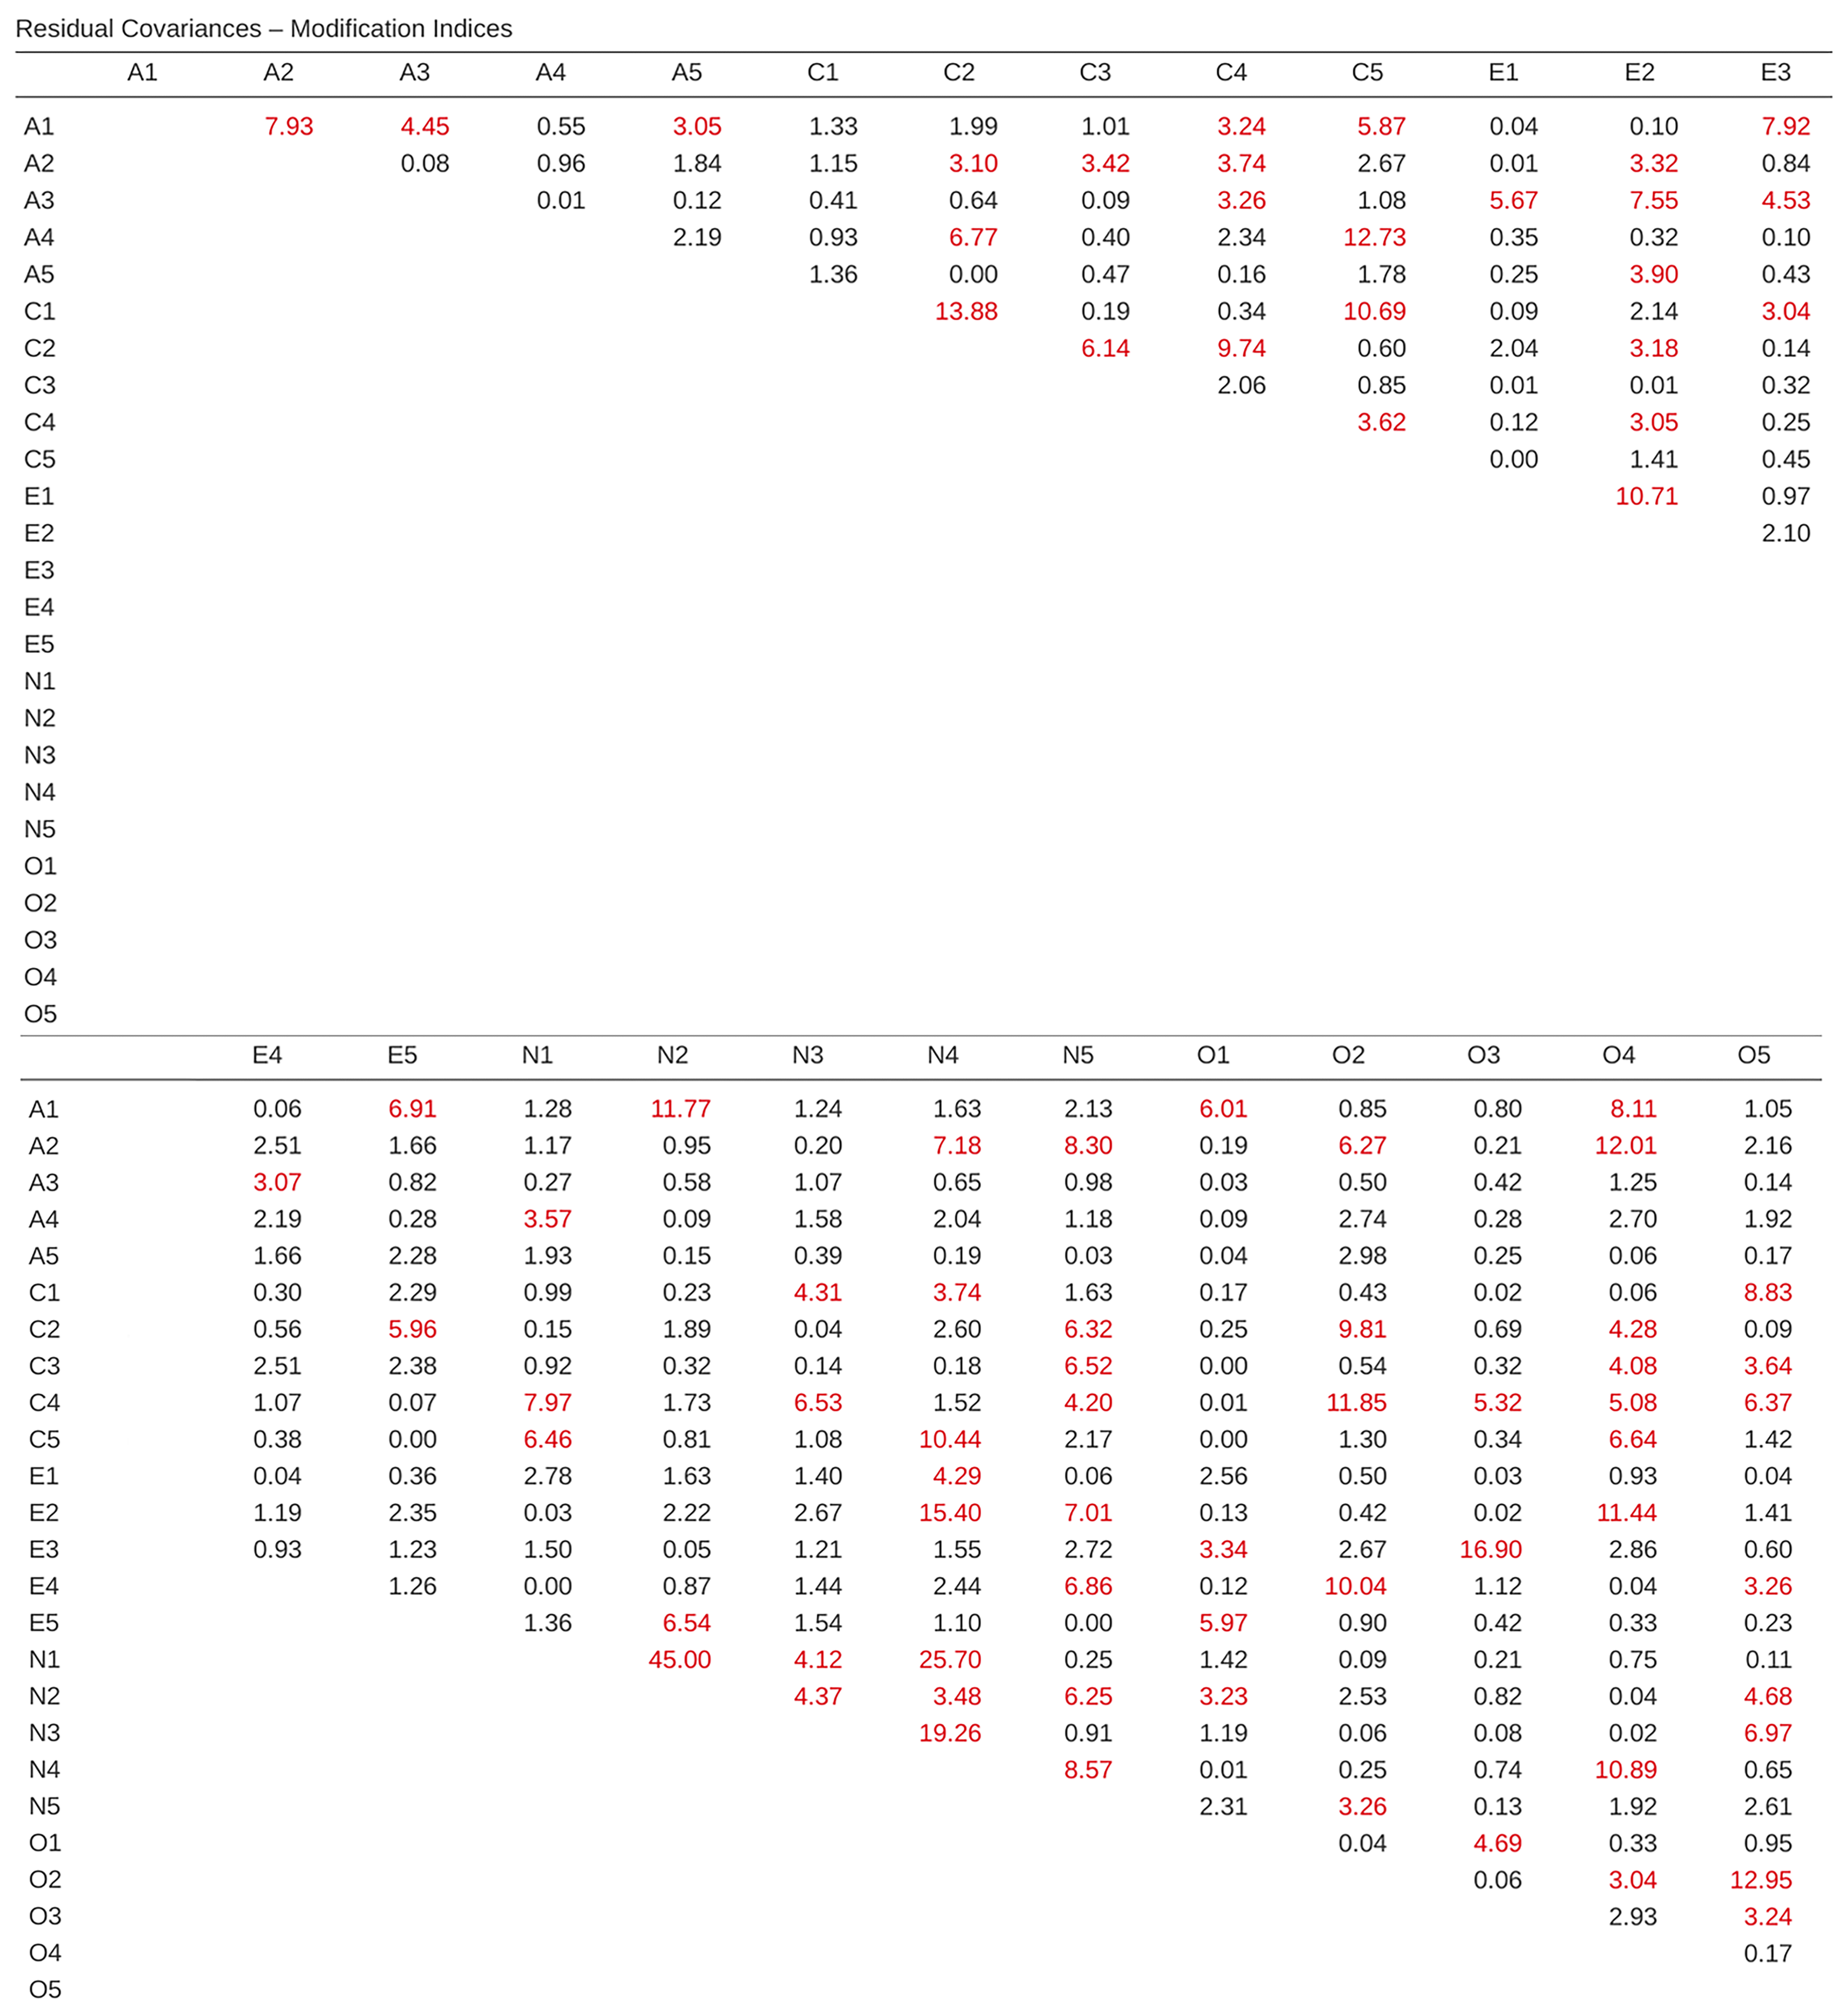
\includegraphics[width=1\textwidth,height=\textheight]{images/fig15-18.png} \hfill{}

\caption{\label{fig-fig15-18}The jamovi CFA Factor Loadings Modification
Indices}

\end{figure}

What we are looking for is the highest modification index (MI) value. We
would then judge whether it makes sense to add that additional term into
the model, using a \emph{post hoc} rationalisation. For example, we can
see in Figure~\ref{fig-fig15-18} that the largest MI for the factor
loadings that are not already in the model is a value of 28.786 for the
loading of N4 (``Often feel blue'') onto the latent factor Extraversion.
This indicates that if we add this path into the model then the
chi-square value will reduce by around the same amount.

But in our model adding this path arguably doesn't really make any
theoretical or methodological sense, so it's not a good idea (unless you
can come up with a persuasive argument that ``Often feel blue'' measures
both Neuroticism and Extraversion). I can't think of a good reason. But,
for the sake of argument, let's pretend it does make some sense and add
this path into the model. Go back to the CFA analysis window (see
Figure~\ref{fig-fig15-14}) and add N4 into the Extraversion factor. The
results of the CFA will now change (not shown); the chi-square has come
down to around 709 (a drop of around 30, roughly similar to the size of
the MI) and the other fit indices have also improved, though only a bit.
But it's not enough: it's still not a good fitting model.

If you do find yourself adding new parameters to a model using the MI
values then always re-check the MI tables after each new addition, as
the MIs are refreshed each time.

There is also a Table of Residual Covariance Modification Indices
produced by jamovi (Figure~\ref{fig-fig15-19}). In other words, a table
showing which correlated errors, if added to the model, would improve
the model fit the most. It's a good idea to look across both MI tables
at the same time, spot the largest MI, think about whether the addition
of the suggested parameter can be reasonably justified and, if it can,
add it to the model. And then you can start again looking for the
biggest MI in the re-calculated results.

\begin{figure}

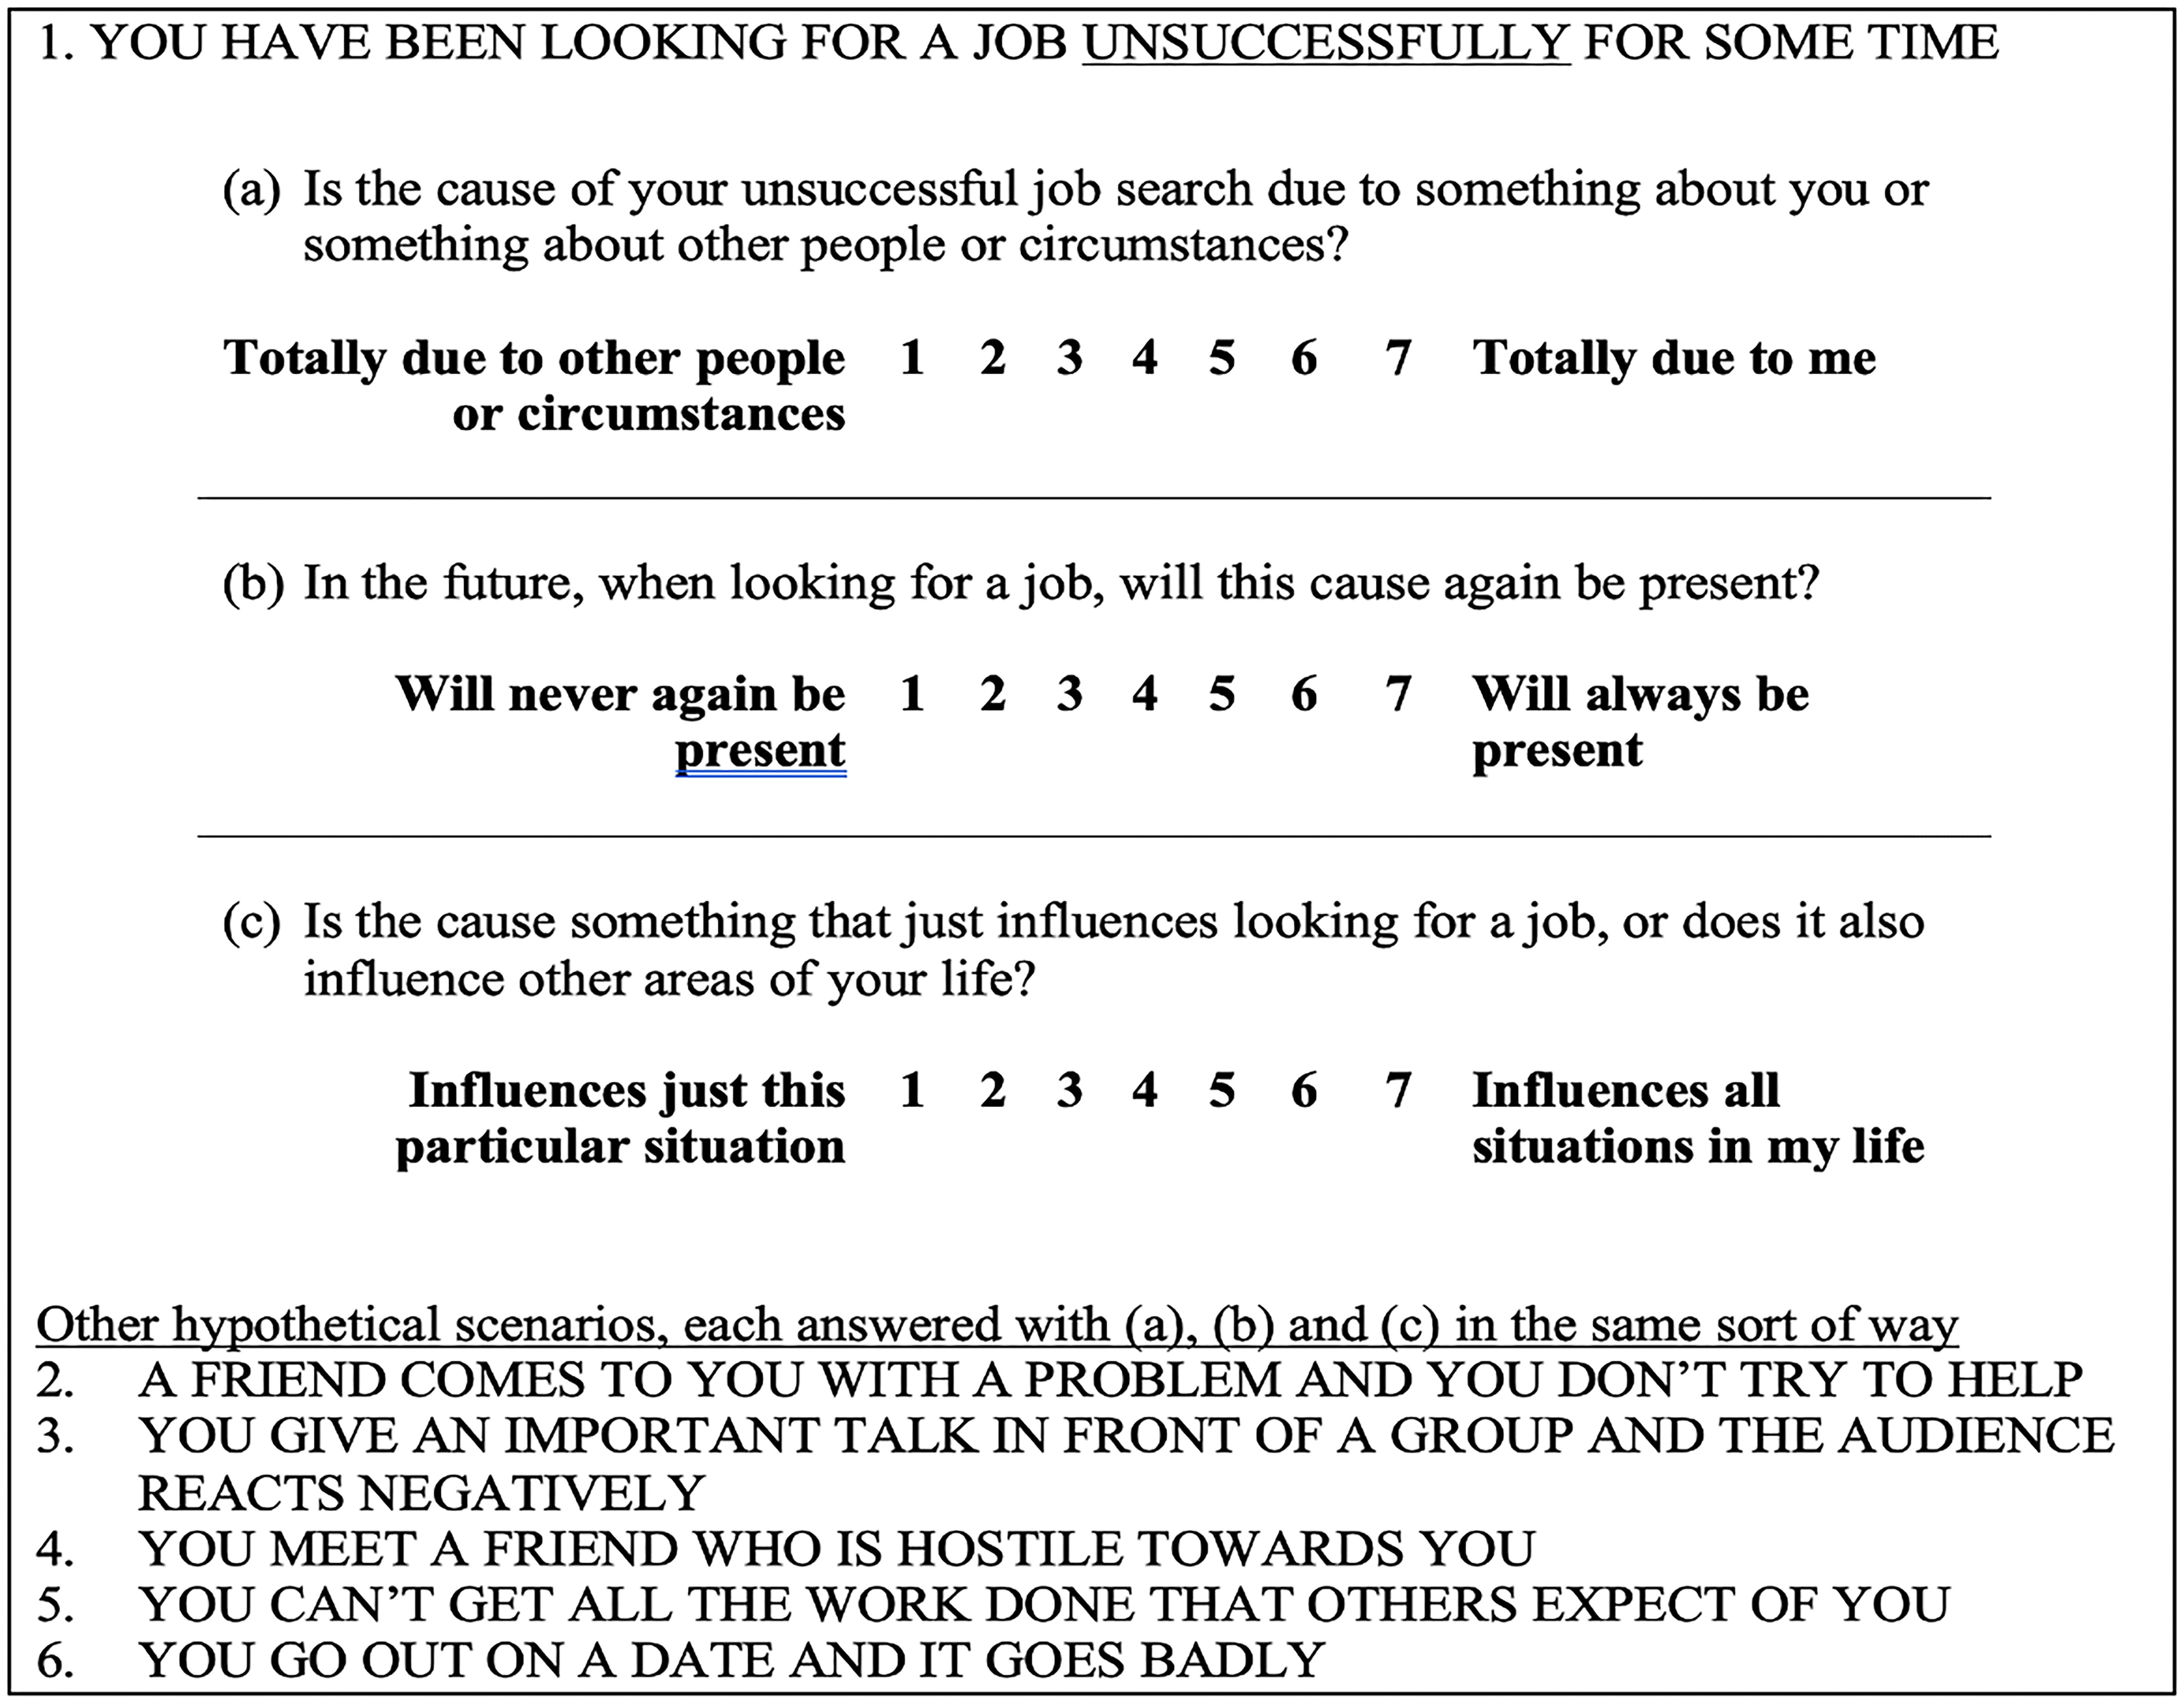
\includegraphics[width=0.6\textwidth,height=\textheight]{images/fig15-19.png} \hfill{}

\caption{\label{fig-fig15-19}Residual Covariance Modification Indices
produced by jamovi}

\end{figure}

You can keep going this way for as long as you like, adding parameters
to the model based on the largest MI, and eventually you will achieve a
satisfactory fit. But there will also be a strong possibility that in
doing this you will have created a monster! A model that is ugly and
deformed and doesn't have any theoretical sense or purity. In other
words, be very careful!

So far, we have checked out the factor structure obtained in the EFA
using a second sample and CFA. Unfortunately, we didn't find that the
factor structure from the EFA was confirmed in the CFA, so it's back to
the drawing board as far as the development of this personality scale
goes.

Although we could have tweaked the CFA using modification indexes, there
really were not any good reasons (that I could think of) for these
suggested additional factor loadings or residual covariances to be
included. However, sometimes there is a good reason for residuals to be
allowed to co-vary (or correlate), and a good example of this is shown
in the next section on
\protect\hyperlink{multi-trait-multi-method-cfa}{Multi-Trait
Multi-Method CFA}. Before we do that, let's cover how to report the
results of a CFA.

\hypertarget{reporting-a-cfa}{%
\subsection{Reporting a CFA}\label{reporting-a-cfa}}

There is not a formal standard way to write up a CFA, and examples tend
to vary by discipline and researcher. That said, there are some fairly
standard pieces of information to include in your write-up:

\begin{enumerate}
\def\labelenumi{\arabic{enumi}.}
\item
  A theoretical and empirical justification for the hypothesized model.
\item
  A complete description of how the model was specified (e.g.~the
  indicator variables for each latent factor, covariances between latent
  variables, and any correlations between error terms). A path diagram,
  like the one in Figure~\ref{fig-fig15-13} would be good to include.
\item
  A description of the sample (e.g.~demographic information, sample
  size, sampling method).
\item
  A description of the type of data used (e.g., nominal, continuous) and
  descriptive statistics.
\item
  Tests of assumptions and estimation method used.
\item
  A description of missing data and how the missing data were handled.
\item
  The software and version used to fit the model.
\item
  Measures, and the criteria used, to judge model fit.
\item
  Any alterations made to the original model based on model fit or
  modification indices.
\item
  All parameter estimates (i.e., loadings, error variances, latent
  (co)variances) and their standard errors, probably in a table.
\end{enumerate}

\hypertarget{multi-trait-multi-method-cfa}{%
\section{Multi-Trait Multi-Method
CFA}\label{multi-trait-multi-method-cfa}}

In this section we're going to consider how different measurement
techniques or questions can be an important source of data variability,
known as \textbf{method variance}. To do this, we'll use another
psychological data set, one that contains data on ``attributional
style''.

The Attributional Style Questionnaire (ASQ) was used (Hewitt et al.,
2004) to collect psychological wellbeing data from young people in the
United Kingdom and New Zealand. They measured attributional style for
negative events, which is how people habitually explain the cause of bad
things that happen to them (Peterson \& Seligman, 1984). The
attributional style questionnaire (ASQ) measures three aspects of
attributional style:

\begin{itemize}
\item
  Internality is the extent to which a person believes that the cause of
  a bad event is due to his/her own actions.
\item
  Stability refers to the extent to which a person habitually believes
  the cause of a bad event is stable across time.
\item
  Globality refers to the extent to which a person habitually believes
  that the cause of a bad event in one area will affect other areas of
  their lives.
\end{itemize}

There are six hypothetical scenarios and for each scenario respondents
answer a question aimed at (a) internality, (b) stability and (c)
globality. So there are \(6 \times 3 = 18\) items overall. See
Figure~\ref{fig-fig15-20} for more details.

\begin{figure}

\includegraphics[width=1\textwidth,height=\textheight]{images/fig15-20.png} \hfill{}

\caption{\label{fig-fig15-20}The Attributional Style Questionnaire (ASQ)
for negative events}

\end{figure}

Researchers are interested in checking their data to see whether there
are some underlying latent factors that are measured reasonably well by
the 18 observed variables in the ASQ.

First, they try EFA with these 18 variables (not shown), but no matter
how they extract or rotate, they can't find a good factor solution.
Their attempt to identify underlying latent factors in the Attributional
Style Questionnaire (ASQ) proved fruitless. If you get results like this
then either your theory is wrong (there is no underlying latent factor
structure for attributional style, which is possible), the sample is not
relevant (which is unlikely given the size and characteristics of this
sample of young adults from the United Kingdom and New Zealand), or the
analysis was not the right tool for the job. We're going to look at this
third possibility.

Remember that there were three dimensions measured in the ASQ:
Internality, Stability and Globality, each measured by six questions as
shown in Figure~\ref{fig-fig15-21}.

What if, instead of doing an analysis where we see how the data goes
together in an exploratory sense, we instead impose a structure, like in
Figure~\ref{fig-fig15-21}, on the data and see how well the data fits
our pre-specified structure. In this sense, we are undertaking a
confirmatory analysis, to see how well a pre-specified model is
confirmed by the observed data.

A straightforward confirmatory factor analysis (CFA) of the ASQ would
therefore specify three latent factors as shown in the columns of
Figure~\ref{fig-fig15-27}, each measured by six observed variables.

\begin{figure}

\includegraphics[width=1\textwidth,height=\textheight]{images/fig15-21.png} \hfill{}

\caption{\label{fig-fig15-21}Six questions on the ASQ for each of the
Internality, Stability and Globality dimensions}

\end{figure}

We could depict this as in the diagram in Figure~\ref{fig-fig15-22},
which shows that each variable is a measure of an underlying latent
factor. For example INT1 is predicted by the underlying latent factor
Internality. And because INT1 is not a perfect measure of the
Internality factor, there is an error term, e1, associated with it. In
other words, e1 represents the variance in INT1 that is not accounted
for by the Internality factor. This is sometimes called ``measurement
error''.

\begin{figure}

\includegraphics[width=1\textwidth,height=\textheight]{images/fig15-22.png} \hfill{}

\caption{\label{fig-fig15-22}Initial pre-specification of latent factor
structure for the ASQ}

\end{figure}

The next step is to consider whether the latent factors should be
allowed to correlate in our model. As mentioned earlier, in the
psychological and behavioural sciences constructs are often related to
each other, and we also think that Internality, Stability, and Globality
might be correlated with each other, so in our model we should allow
these latent factors to co-vary, as shown in Figure~\ref{fig-fig15-23}.

\begin{figure}

\includegraphics[width=1\textwidth,height=\textheight]{images/fig15-23.png} \hfill{}

\caption{\label{fig-fig15-23}Final pre-specification of latent factor
structure for the ASQ, including latent factor correlations, and shared
method error term correlations for the observed variable INT1, STAB1 and
GLOB1, in a CFA MTMM model. For clarity, other pre-specified error term
correlations are not shown}

\end{figure}

At the same time, we should consider whether there is any good,
systematic, reason for some of the error terms to be correlated with
each other. Thinking back to the ASQ questions, there were three
different sub-questions (a, b and c) for each main question (1-6). Q1
was about unsuccessful job hunting and it is plausible that this
question has some distinctive artefactual or methodological aspects over
and above the other questions (2-5), something to do with job hunting
perhaps. Similarly, Q2 was about not helping a friend with a problem,
and there may be some distinctive artefactual or methodological aspects
to do with not helping a friend that is not present in the other
questions (1, and 3-5).

So, as well as multiple factors, we also have multiple methodological
features in the ASQ, where each of Questions 1-6 has a slightly
different ``method'', but each ``method'' is shared across the
sub-questions a, b and c.~In order to incorporate these different
methodological features into the model we can specify that certain error
terms are correlated with each other. For example, the errors associated
with INT1, STAB1 and GLOB1 should be correlated with each other to
reflect the distinct and shared methodological variance of Q1a, Q1b and
Q1c. Looking at Figure~\ref{fig-fig15-21}, this means that as well as
the latent factors represented by the columns, we will have correlated
measurement errors for the variables in each row of the Table.

Whilst a basic CFA model like the one shown in Figure~\ref{fig-fig15-22}
could be tested against our observed data, we have in fact come up with
a more sophisticated model, as shown in the diagram in
Figure~\ref{fig-fig15-23}. This more sophisticated CFA model is known as
a \textbf{Multi-Trait Multi-Method (MTMM)} model, and it is the one we
will test in jamovi.

\hypertarget{mtmm-cfa-in-jamovi}{%
\subsection{MTMM CFA in jamovi}\label{mtmm-cfa-in-jamovi}}

Open up the \emph{ASQ.csv} file and check that the 18 variables (six
``Internality'', six ``Stability'' and six ``Globality'' variables) are
specified as continuous variables.

To perform MTMM CFA in jamovi:

\begin{itemize}
\item
  Select Factor - Confirmatory Factor Analysis from the main jamovi
  button bar to open the CFA analysis window
  (Figure~\ref{fig-fig15-24}).
\item
  Select the 6 INT variables and transfer them into the `Factors' box
  and give them the label ``Internality''.
\item
  Create a new Factor in the `Factors' box and label it ``Stability''.
  Select the 6 STAB variables and transfer them into the `Factors' box
  under the ``Stability'' label.
\item
  Create another new Factor in the `Factors' box and label it
  ``Globality''. Select the 6 GLOB variables and transfer them into the
  `Factors' box under the ``Globality'' label.
\item
  Open up the Residual Covariances options, and for each of our
  pre-specified correlations move the associated variables across into
  the `Residual Covariances' box on the right. For example, highlight
  both INT1 and STAB1 and then click the arrow to move these across. Now
  do the same for INT1 and GLOB1, for STAB1 and GLOB1, for INT2 and
  STAB2, for INT2 and GLOB2, for STAB2 and GLOB2, for INT3 and STAB3,
  and so on.
\item
  Check other appropriate options, the defaults are ok for this initial
  work through, though you might want to check the ``Path diagram''
  option under `Plots' to see jamovi produce a (fairly) similar diagram
  to our Figure~\ref{fig-fig15-23}, and including all the error term
  correlations that we have added above.
\end{itemize}

\begin{figure}

\includegraphics[width=1\textwidth,height=\textheight]{images/fig15-24.png} \hfill{}

\caption{\label{fig-fig15-24}The jamovi CFA analysis window}

\end{figure}

Once we have set up the analysis we can turn our attention to the jamovi
results window and see what's what. The first thing to look at is
``Model fit'' as this tells us how good a fit our model is to the
observed data (Figure~\ref{fig-fig15-25}). NB in our model only the
pre-specified covariances are estimated, everything else is set to zero,
so model fit is testing both whether the pre-specified ``free''
parameters are not zero, and conversely whether the other relationships
in the data -- the ones we have not specified in the model -- can be
held at zero.

\begin{figure}

\includegraphics[width=1\textwidth,height=\textheight]{images/fig15-25.png} \hfill{}

\caption{\label{fig-fig15-25}The jamovi CFA Model Fit results for our
CFA MTMM model}

\end{figure}

Looking at Figure~\ref{fig-fig15-25} we can see that the chi-square
value is highly significant, which is not a surprise given the large
sample size (N = 2748). The CFI is 0.98 and the TLI is also 0.98,
indicating a very good fit. The RMSEA is 0.02 with a 90\% confidence
interval from 0.02 to 0.02 -- pretty tight!

Overall, I think we can be satisfied that our pre-specified model is a
very good fit to the observed data, lending support to our MTMM model
for the ASQ.

We can now go on to look at the factor loadings and the factor
covariance estimates, as in Figure~\ref{fig-fig15-26}. Often the
standardized estimates are easier to interpret, and these can be
specified under the `Estimates' option. These tables can usefully be
incorporated into a written report or scientific article.

\begin{figure}

\includegraphics[width=1\textwidth,height=\textheight]{images/fig15-26.png} \hfill{}

\caption{\label{fig-fig15-26}The jamovi CFA Factor Loadings and
Covariances tables for our CFA MTMM model}

\end{figure}

You can see from Figure~\ref{fig-fig15-26} that all of our pre-specified
factor loadings and factor covariances are significantly different from
zero. In other words, they all seem to be making a useful contribution
to the model.

We've been pretty lucky with this analysis, getting a very good fit on
our first attempt!

\hypertarget{sec-Internal-consistency-reliability-analysis}{%
\section{Internal consistency reliability
analysis}\label{sec-Internal-consistency-reliability-analysis}}

After you have been through the process of initial scale development
using EFA and CFA, you should have reached a stage where the scale holds
up pretty well using CFA with different samples. One thing that you
might also be interested in at this stage is to see how well the factors
are measured using a scale that combines the observed variables.

In psychometrics we use reliability analysis to provide information
about how consistently a scale measures a psychological construct (See
earlier section on
\textbf{?@sec-Assessing-the-reliability-of-a-measurement}).
\textbf{Internal consistency} is what we are concerned with here, and
that refers to the consistency across all the individual items that make
up a measurement scale. So, if we have \(V1, V2, V3, V4\) and \(V5\) as
observed item variables, then we can calculate a statistic that tells us
how internally consistent these items are in measuring the underlying
construct.

A popular statistic used to check the internal consistency of a scale is
\textbf{Cronbach's alpha} (Chronbach, 1951). Cronbach's alpha is a
measure of equivalence (whether different sets of scale items would give
the same measurement outcomes). Equivalence is tested by dividing the
scale items into two groups (a ``split-half'') and seeing whether
analysis of the two parts gives comparable results. Of course, there are
many ways a set of items could be split, but if all possible splits are
made then it is possible to produce a statistic that reflects the
overall pattern of split-half coefficients. Cronbach's alpha
(\(\alpha\)) is such a statistic: a function of all the split-half
coefficients for a scale. If a set of items that measure a construct
(e.g.~an Extraversion scale) has an \(\alpha\) of \(0.80\), then the
proportion of error variance in the scale is \(0.20\). In other words, a
scale with an \(\alpha\) of \(0.80\) includes approximately 20\% error.

BUT, (and that's a BIG ``BUT''), Cronbach's alpha is not a measure of
unidimensionality (i.e.~an indicator that a scale is measuring a single
factor or construct rather than multiple related constructs). Scales
that are multidimensional will cause alpha to be under-estimated if not
assessed separately for each dimension, but high values for alpha are
not necessarily indicators of unidimensionality. So, an \(\alpha\) of
0.80 does not mean that 80\% of a single underlying construct is
accounted for. It could be that the 80\% comes from more than one
underlying construct. That's why EFA and CFA are useful to do first.

Further, another feature of \(\alpha\) is that it tends to be sample
specific: it is not a characteristic of the scale, but rather a
characteristic of the sample in which the scale has been used. A biased,
unrepresentative, or small sample could produce a very different
\(\alpha\) coefficient than a large, representative sample. \(\alpha\)
can even vary from large sample to large sample. Nevertheless, despite
these limitations, Cronbach's \(\alpha\) has been popular in Psychology
for estimating internal consistency reliability. It's pretty easy to
calculate, understand and interpret, and therefore it can be a useful
initial check on scale performance when you administer a scale with a
different sample, from a different setting or population, for example.

An alternative is \textbf{McDonald's omega} (\(\omega\)), and jamovi
also provides this statistic. Whereas \(\alpha\) makes the following
assumptions: (a) no residual correlations, (b) items have identical
loadings, and (c) the scale is unidimensional, \(\omega\) does not and
is therefore a more robust reliability statistic. If these assumptions
are not violated then \(\alpha\) and \(\omega\) will be similar, but if
they are then \(\omega\) is to be preferred.

Sometimes a threshold for \(\alpha\) or \(\omega\) is provided,
suggesting a ``good enough'' value. This might be something like
\(\alpha\)s of \(0.70\) or \(0.80\) representing ``acceptable'' and
``good'' reliability, respectively. However, this does depend on what
exactly the scale is supposed to be measuring, so thresholds like this
should be used cautiously. It could be better to simply state that an
\(\alpha\) or \(\omega\) of \(0.70\) is associated with 30\% error
variance in a scale, and an \(\alpha\) or \(\omega\) of \(0.80\) is
associated with 20\%.

Can \(\alpha\) be too high? Probably: if you are getting an \(\alpha\)
coefficient above \(0.95\) then this indicates high inter-correlations
between the items and that there might be too much overly redundant
specificity in the measurement, with a risk that the construct being
measured is perhaps overly narrow.

\hypertarget{reliability-analysis-in-jamovi}{%
\subsection{Reliability analysis in
jamovi}\label{reliability-analysis-in-jamovi}}

We have a third sample of personality data to use to undertake
reliability analysis: in the bfi\_sample3.csv file. Once again, check
that the 25 personality item variables are coded as continuous. To
perform reliability analysis in jamovi:

\begin{itemize}
\item
  Select Factor - Reliability Analysis from the main jamovi button bar
  to open the reliability analysis window (Figure~\ref{fig-fig15-27}).
\item
  Select the 5 A variables and transfer them into the `Items' box.
\item
  Under the ``Reverse Scaled Items'' option, select variable A1 in the
  ``Normal Scaled Items'' box and move it across to the ``Reverse Scaled
  Items'' box.
\item
  Check other appropriate options, as in Figure~\ref{fig-fig15-27}.
\end{itemize}

\begin{figure}

\includegraphics[width=1\textwidth,height=\textheight]{images/fig15-27.png} \hfill{}

\caption{\label{fig-fig15-27}The jamovi Reliability Analysis window}

\end{figure}

Once done, look across at the jamovi results window. You should see
something like Figure~\ref{fig-fig15-28}. This tells us that the
Cronbach's \(\alpha\) coefficient for the Agreeableness scale is 0.72.
This means that just under 30\% of the Agreeableness scale score is
error variance. McDonald's \(\omega\) is also given, and this is 0.74,
not much different from \(\alpha\).

\begin{figure}

\includegraphics[width=1\textwidth,height=\textheight]{images/fig15-28.png} \hfill{}

\caption{\label{fig-fig15-28}The jamovi Reliability Analysis results for
the Agreeableness factor}

\end{figure}

We can also check how \(\alpha\) or \(\omega\) can be improved if a
specific item is dropped from the scale. For example, \(\alpha\) would
increase to 0.74 and \(\omega\) to 0.75 if we dropped item A1. This
isn't a big increase, so probably not worth doing.

The process of calculating and checking scale statistics (\(\alpha\) and
\(\omega\)) is the same for all the other scales, and they all had
similar reliability estimates apart from Openness. For Openness, the
amount of error variance in the Scale score is around 40\%, which is
high and indicates that Openness is substantially less consistent as a
reliable measure of a personality attribute than the other personality
scales.

\hypertarget{summary-1}{%
\section{Summary}\label{summary-1}}

In this chapter on factor analysis and related techniques we have
introduced and demonstrated statistical analyses that assess the pattern
of relationships in a data set. Specifically, we have covered:

\begin{itemize}
\item
  \protect\hyperlink{exploratory-factor-analysis}{Exploratory Factor
  Analysis} (EFA). EFA is a statistical technique for identifying
  underlying latent factors in a data set. Each observed variable is
  conceptualised as representing the latent factor to some extent,
  indicated by a factor loading. Researchers also use EFA as a way of
  data reduction, i.e.~identifying observed variables than can be
  combined into new factor variables for subsequent analysis.
\item
  \protect\hyperlink{principal-component-analysis}{Principal Component
  Analysis} (PCA) is a data reduction technique which, strictly
  speaking, does not identify underlying latent factors. Instead, PCA
  simply produces a linear combination of observed variables.
\item
  \protect\hyperlink{confirmatory-factor-analysis}{Confirmatory Factor
  Analysis} (CFA). Unlike EFA, with CFA you start with an idea - a model
  - of how the variables in your data are related to each other. You
  then test your model against the observed data and assess how good a
  fit the model is to the data.
\item
  In \protect\hyperlink{multi-trait-multi-method-cfa}{Multi-Trait
  Multi-Method CFA} (MTMM CFA), both latent factor and method variance
  are included in the model in an approach that is useful when there are
  different methodological approaches used and therefore method variance
  is an important consideration.
\item
  \protect\hyperlink{sec-Internal-consistency-reliability-analysis}{Internal
  consistency reliability analysis}. This form of reliability analysis
  tests how consistently a scale measures a measurement (psychological)
  construct.
\end{itemize}

\part{Endings, alternatives and prospects}

\hypertarget{sec-Bayesian-statistics}{%
\chapter{Bayesian statistics}\label{sec-Bayesian-statistics}}

\begin{quote}
\emph{``In our reasonings concerning matter of fact, there are all
imaginable degrees of assurance, from the highest certainty to the
lowest species of moral evidence. A wise man, therefore, proportions his
belief to the evidence.''}\\
-- David Hume\footnote{\url{http://en.wikiquote.org/wiki/David_Hume}.}
\end{quote}

The ideas I've presented to you in this book describe inferential
statistics from the frequentist perspective. I'm not alone in doing
this. In fact, almost every textbook given to undergraduate psychology
students presents the opinions of the frequentist statistician as
\emph{the} theory of inferential statistics, the one true way to do
things. I have taught this way for practical reasons. The frequentist
view of statistics dominated the academic field of statistics for most
of the 20th century, and this dominance is even more extreme among
applied scientists. It was and is current practice among psychologists
to use frequentist methods. Because frequentist methods are ubiquitous
in scientific papers, every student of statistics needs to understand
those methods, otherwise they will be unable to make sense of what those
papers are saying! Unfortunately, in my opinion at least, the current
practice in psychology is often misguided, and the reliance on
frequentist methods is partly to blame. In this chapter I explain why I
think this and provide an introduction to Bayesian statistics, an
approach that I think is generally superior to the orthodox approach.

This chapter comes in two parts. In the first three sections I talk
about what Bayesian statistics are all about, covering the basic
mathematical rules for how it works as well as an explanation for why I
think the Bayesian approach is so useful. Afterwards, I provide a brief
overview of how you can do{[}Bayesian t-tests{]}.

\hypertarget{probabilistic-reasoning-by-rational-agents}{%
\section{Probabilistic reasoning by rational
agents}\label{probabilistic-reasoning-by-rational-agents}}

From a Bayesian perspective statistical inference is all about
\emph{belief revision}. I start out with a set of candidate hypotheses,
\(h\), about the world. I don't know which of these hypotheses is true,
but do I have some beliefs about which hypotheses are plausible and
which are not. When I observe the data, \(d\), I have to revise those
beliefs. If the data are consistent with a hypothesis, my belief in that
hypothesis is strengthened. If the data are inconsistent with the
hypothesis, my belief in that hypothesis is weakened. That's it! At the
end of this section I'll give a precise description of how Bayesian
reasoning works, but first I want to work through a simple example in
order to introduce the key ideas. Consider the following reasoning
problem.

\begin{quote}
\emph{I'm carrying an umbrella. Do you think it will rain?}
\end{quote}

In this problem I have presented you with a single piece of data (\(d\)
= I'm carrying the umbrella), and I'm asking you to tell me your belief
or hypothesis about whether it's raining. You have two alternatives,
\(h\): either it will rain today or it will not. How should you solve
this problem?

\hypertarget{priors-what-you-believed-before}{%
\subsection{Priors: what you believed
before}\label{priors-what-you-believed-before}}

The first thing you need to do is ignore what I told you about the
umbrella, and write down your pre-existing beliefs about rain. This is
important. If you want to be honest about how your beliefs have been
revised in the light of new evidence (data) then you must say something
about what you believed before those data appeared! So, what might you
believe about whether it will rain today? You probably know that I live
in Australia and that much of Australia is hot and dry. The city of
Adelaide where I live has a Mediterranean climate, very similar to
southern California, southern Europe or northern Africa. I'm writing
this in January and so you can assume it's the middle of summer. In
fact, you might have decided to take a quick look on
Wikipedia\footnote{http://en.wikipedia.org/wiki/Climate\_of\_Adelaide}
and discovered that Adelaide gets an average of 4.4 days of rain across
the 31 days of January. Without knowing anything else, you might
conclude that the probability of January rain in Adelaide is about 15\%,
and the probability of a dry day is 85\% (see Table~\ref{tbl-tab16-1}).
If this is really what you believe about Adelaide rainfall (and now that
I've told it to you I'm betting that this really is what you believe)
then what I have written here is your \textbf{prior distribution},
written \(P(h)\).

\hypertarget{tbl-tab16-1}{}
 
  \providecommand{\huxb}[2]{\arrayrulecolor[RGB]{#1}\global\arrayrulewidth=#2pt}
  \providecommand{\huxvb}[2]{\color[RGB]{#1}\vrule width #2pt}
  \providecommand{\huxtpad}[1]{\rule{0pt}{#1}}
  \providecommand{\huxbpad}[1]{\rule[-#1]{0pt}{#1}}

\begin{table}[ht]
\caption{\label{tbl-tab16-1}How likely is it to rain in Adelaide - pre-existing beliefs based on
knowledge of average January rainfall }\tabularnewline

\begin{centerbox}
\begin{threeparttable}
\setlength{\tabcolsep}{0pt}
\begin{tabularx}{0.9\textwidth}{p{0.45\textwidth} p{0.45\textwidth}}


\hhline{>{\huxb{0, 0, 0}{0.4}}->{\huxb{0, 0, 0}{0.4}}-}
\arrayrulecolor{black}

\multicolumn{1}{!{\huxvb{0, 0, 0}{0}}p{0.45\textwidth}!{\huxvb{0, 0, 0}{0}}}{\hspace{0pt}\parbox[b]{0.45\textwidth-0pt-12pt}{\huxtpad{2pt + 1em}\centering \textbf{Hypothesis}\huxbpad{2pt}}} &
\multicolumn{1}{p{0.45\textwidth}!{\huxvb{0, 0, 0}{0}}}{\hspace{12pt}\parbox[b]{0.45\textwidth-12pt-0pt}{\huxtpad{2pt + 1em}\centering \textbf{Degree of Belief}\huxbpad{2pt}}} \tabularnewline[-0.5pt]


\hhline{>{\huxb{0, 0, 0}{0.4}}->{\huxb{0, 0, 0}{0.4}}-}
\arrayrulecolor{black}

\multicolumn{1}{!{\huxvb{0, 0, 0}{0}}p{0.45\textwidth}!{\huxvb{0, 0, 0}{0}}}{\hspace{0pt}\parbox[b]{0.45\textwidth-0pt-12pt}{\huxtpad{2pt + 1em}\centering Rainy day\huxbpad{2pt}}} &
\multicolumn{1}{p{0.45\textwidth}!{\huxvb{0, 0, 0}{0}}}{\hspace{12pt}\parbox[b]{0.45\textwidth-12pt-0pt}{\huxtpad{2pt + 1em}\centering 0.15\huxbpad{2pt}}} \tabularnewline[-0.5pt]


\hhline{}
\arrayrulecolor{black}

\multicolumn{1}{!{\huxvb{0, 0, 0}{0}}p{0.45\textwidth}!{\huxvb{0, 0, 0}{0}}}{\hspace{0pt}\parbox[b]{0.45\textwidth-0pt-12pt}{\huxtpad{2pt + 1em}\centering Dry day\huxbpad{2pt}}} &
\multicolumn{1}{p{0.45\textwidth}!{\huxvb{0, 0, 0}{0}}}{\hspace{12pt}\parbox[b]{0.45\textwidth-12pt-0pt}{\huxtpad{2pt + 1em}\centering 0.85\huxbpad{2pt}}} \tabularnewline[-0.5pt]


\hhline{>{\huxb{0, 0, 0}{0.4}}->{\huxb{0, 0, 0}{0.4}}-}
\arrayrulecolor{black}
\end{tabularx} 

\end{threeparttable}\par\end{centerbox}

\end{table}
 

\hypertarget{likelihoods-theories-about-the-data}{%
\subsection{Likelihoods: theories about the
data}\label{likelihoods-theories-about-the-data}}

To solve the reasoning problem you need a theory about my behaviour.
When does Danielle carry an umbrella? You might guess that I'm not a
complete idiot,\footnote{It's a leap of faith, I know, but let's run
  with it okay?} and I try to carry umbrellas only on rainy days. On the
other hand, you also know that I have young kids, and you wouldn't be
all that surprised to know that I'm pretty forgetful about this sort of
thing. Let's suppose that on rainy days I remember my umbrella about
30\% of the time (I really am awful at this). But let's say that on dry
days I'm only about 5\% likely to be carrying an umbrella. So you might
write this out as in Table~\ref{tbl-tab16-2}.

\hypertarget{tbl-tab16-2}{}
 
  \providecommand{\huxb}[2]{\arrayrulecolor[RGB]{#1}\global\arrayrulewidth=#2pt}
  \providecommand{\huxvb}[2]{\color[RGB]{#1}\vrule width #2pt}
  \providecommand{\huxtpad}[1]{\rule{0pt}{#1}}
  \providecommand{\huxbpad}[1]{\rule[-#1]{0pt}{#1}}

\begin{table}[ht]
\caption{\label{tbl-tab16-2}How likely am I to be carrying an umbrella on rainy and dry days }\tabularnewline

\begin{centerbox}
\begin{threeparttable}
\setlength{\tabcolsep}{0pt}
\begin{tabularx}{0.9\textwidth}{p{0.3\textwidth} p{0.3\textwidth} p{0.3\textwidth}}


\hhline{>{\huxb{0, 0, 0}{0.4}}->{\huxb{0, 0, 0}{0.4}}->{\huxb{0, 0, 0}{0.4}}-}
\arrayrulecolor{black}

\multicolumn{1}{!{\huxvb{0, 0, 0}{0}}p{0.3\textwidth}!{\huxvb{0, 0, 0}{0}}}{\hspace{0pt}\parbox[b]{0.3\textwidth-0pt-12pt}{\huxtpad{2pt + 1em}\centering \textbf{}\huxbpad{2pt}}} &
\multicolumn{1}{p{0.3\textwidth}!{\huxvb{0, 0, 0}{0}}}{\hspace{12pt}\parbox[b]{0.3\textwidth-12pt-12pt}{\huxtpad{2pt + 1em}\centering \textbf{Data}\huxbpad{2pt}}} &
\multicolumn{1}{p{0.3\textwidth}!{\huxvb{0, 0, 0}{0}}}{\hspace{12pt}\parbox[b]{0.3\textwidth-12pt-0pt}{\huxtpad{2pt + 1em}\centering \textbf{Data}\huxbpad{2pt}}} \tabularnewline[-0.5pt]


\hhline{>{\huxb{0, 0, 0}{0.4}}->{\huxb{0, 0, 0}{0.4}}->{\huxb{0, 0, 0}{0.4}}-}
\arrayrulecolor{black}

\multicolumn{1}{!{\huxvb{0, 0, 0}{0}}p{0.3\textwidth}!{\huxvb{0, 0, 0}{0}}}{\hspace{0pt}\parbox[b]{0.3\textwidth-0pt-12pt}{\huxtpad{2pt + 1em}\centering Hypothesis\huxbpad{2pt}}} &
\multicolumn{1}{p{0.3\textwidth}!{\huxvb{0, 0, 0}{0}}}{\hspace{12pt}\parbox[b]{0.3\textwidth-12pt-12pt}{\huxtpad{2pt + 1em}\centering Umbrella\huxbpad{2pt}}} &
\multicolumn{1}{p{0.3\textwidth}!{\huxvb{0, 0, 0}{0}}}{\hspace{12pt}\parbox[b]{0.3\textwidth-12pt-0pt}{\huxtpad{2pt + 1em}\centering No umbrella\huxbpad{2pt}}} \tabularnewline[-0.5pt]


\hhline{}
\arrayrulecolor{black}

\multicolumn{1}{!{\huxvb{0, 0, 0}{0}}p{0.3\textwidth}!{\huxvb{0, 0, 0}{0}}}{\hspace{0pt}\parbox[b]{0.3\textwidth-0pt-12pt}{\huxtpad{2pt + 1em}\centering Rainy day\huxbpad{2pt}}} &
\multicolumn{1}{p{0.3\textwidth}!{\huxvb{0, 0, 0}{0}}}{\hspace{12pt}\parbox[b]{0.3\textwidth-12pt-12pt}{\huxtpad{2pt + 1em}\centering 0.30\huxbpad{2pt}}} &
\multicolumn{1}{p{0.3\textwidth}!{\huxvb{0, 0, 0}{0}}}{\hspace{12pt}\parbox[b]{0.3\textwidth-12pt-0pt}{\huxtpad{2pt + 1em}\centering 0.70\huxbpad{2pt}}} \tabularnewline[-0.5pt]


\hhline{}
\arrayrulecolor{black}

\multicolumn{1}{!{\huxvb{0, 0, 0}{0}}p{0.3\textwidth}!{\huxvb{0, 0, 0}{0}}}{\hspace{0pt}\parbox[b]{0.3\textwidth-0pt-12pt}{\huxtpad{2pt + 1em}\centering Dry day\huxbpad{2pt}}} &
\multicolumn{1}{p{0.3\textwidth}!{\huxvb{0, 0, 0}{0}}}{\hspace{12pt}\parbox[b]{0.3\textwidth-12pt-12pt}{\huxtpad{2pt + 1em}\centering 0.05\huxbpad{2pt}}} &
\multicolumn{1}{p{0.3\textwidth}!{\huxvb{0, 0, 0}{0}}}{\hspace{12pt}\parbox[b]{0.3\textwidth-12pt-0pt}{\huxtpad{2pt + 1em}\centering 0.95\huxbpad{2pt}}} \tabularnewline[-0.5pt]


\hhline{>{\huxb{0, 0, 0}{0.4}}->{\huxb{0, 0, 0}{0.4}}->{\huxb{0, 0, 0}{0.4}}-}
\arrayrulecolor{black}
\end{tabularx} 

\end{threeparttable}\par\end{centerbox}

\end{table}
 

It's important to remember that each cell in this table describes your
beliefs about what data \(d\) will be observed, \emph{given} the truth
of a particular hypothesis \(h\). This ``conditional probability'' is
written \(P(d|h)\), which you can read as ``the probability of \(d\)
given \(h\)''. In Bayesian statistics, this is referred to as the
\textbf{likelihood} of the data \(d\) given the hypothesis
\(h\).\footnote{Um. I hate to bring this up, but some statisticians
  would object to me using the word ``likelihood'' here. The problem is
  that the word ``likelihood'' has a very specific meaning in
  frequentist statistics, and it's not quite the same as what it means
  in Bayesian statistics. As far as I can tell Bayesians didn't
  originally have any agreed upon name for the likelihood, and so it
  became common practice for people to use the frequentist terminology.
  This wouldn't have been a problem except for the fact that the way
  that Bayesians use the word turns out to be quite different to the way
  frequentists do. This isn't the place for yet another lengthy history
  lesson but, to put it crudely, when a Bayesian says ``a likelihood
  function'' they're usually referring one of the rows of the table.
  When a frequentist says the same thing, they're referring to the same
  table, but to them ``a likelihood function'' almost always refers to
  one of the columns. This distinction matters in some contexts, but
  it's not important for our purposes.}

\hypertarget{the-joint-probability-of-data-and-hypothesis}{%
\subsection{The joint probability of data and
hypothesis}\label{the-joint-probability-of-data-and-hypothesis}}

At this point all the elements are in place. Having written down the
priors and the likelihood, you have all the information you need to do
Bayesian reasoning. The question now becomes how do we use this
information? As it turns out, there's a very simple equation that we can
use here, but it's important that you understand why we use it, so I'm
going to try to build it up from more basic ideas.

Let's start out with one of the rules of probability theory. I listed it
way back in \textbf{?@tbl-tab7-1}, but I didn't make a big deal out of
it at the time, and you probably ignored it. The rule in question is the
one that talks about the probability that two things are true. In our
example, you might want to calculate the probability that today is rainy
(i.e., hypothesis \(h\) is true) and I'm carrying an umbrella (i.e.,
data \(d\) is observed). The \textbf{joint probability} of the
hypothesis and the data is written \(P(d,h)\), and you can calculate it
by multiplying the prior \(P(h)\) by the likelihood \(P(d|h)\).
Mathematically, we say that

\[P(d,h)=P(d|h)P(h)\]

So, what is the probability that today is a rainy day \emph{and} I
remember to carry an umbrella? As we discussed earlier, the prior tells
us that the probability of a rainy day is 15\%, and the likelihood tells
us that the probability of me remembering my umbrella on a rainy day is
30\%. So the probability that both of these things are true is
calculated by multiplying the two

\[
\begin{split}
P(rainy, umbrella) & = P(umbrella|rainy) \times P(rainy) \\
& = 0.30 \times 0.15 \\
& = 0.045
\end{split}
\]

In other words, before being told anything about what actually happened,
you think that there is a 4.5\% probability that today will be a rainy
day and that I will remember an umbrella. However, there are of course
four possible things that could happen, right? So let's repeat the
exercise for all four. If we do that, we end up with
Table~\ref{tbl-tab16-3}.

\hypertarget{tbl-tab16-3}{}
 
  \providecommand{\huxb}[2]{\arrayrulecolor[RGB]{#1}\global\arrayrulewidth=#2pt}
  \providecommand{\huxvb}[2]{\color[RGB]{#1}\vrule width #2pt}
  \providecommand{\huxtpad}[1]{\rule{0pt}{#1}}
  \providecommand{\huxbpad}[1]{\rule[-#1]{0pt}{#1}}

\begin{table}[ht]
\caption{\label{tbl-tab16-3}Four possibilities combining rain (or not) and umbrella carrying (or
not) }\tabularnewline

\begin{centerbox}
\begin{threeparttable}
\setlength{\tabcolsep}{0pt}
\begin{tabularx}{0.9\textwidth}{p{0.3\textwidth} p{0.3\textwidth} p{0.3\textwidth}}


\hhline{>{\huxb{0, 0, 0}{0.4}}->{\huxb{0, 0, 0}{0.4}}->{\huxb{0, 0, 0}{0.4}}-}
\arrayrulecolor{black}

\multicolumn{1}{!{\huxvb{0, 0, 0}{0}}p{0.3\textwidth}!{\huxvb{0, 0, 0}{0}}}{\hspace{0pt}\parbox[b]{0.3\textwidth-0pt-12pt}{\huxtpad{2pt + 1em}\centering \textbf{}\huxbpad{2pt}}} &
\multicolumn{1}{p{0.3\textwidth}!{\huxvb{0, 0, 0}{0}}}{\hspace{12pt}\parbox[b]{0.3\textwidth-12pt-12pt}{\huxtpad{2pt + 1em}\centering \textbf{Umbrella}\huxbpad{2pt}}} &
\multicolumn{1}{p{0.3\textwidth}!{\huxvb{0, 0, 0}{0}}}{\hspace{12pt}\parbox[b]{0.3\textwidth-12pt-0pt}{\huxtpad{2pt + 1em}\centering \textbf{No-umbrella}\huxbpad{2pt}}} \tabularnewline[-0.5pt]


\hhline{>{\huxb{0, 0, 0}{0.4}}->{\huxb{0, 0, 0}{0.4}}->{\huxb{0, 0, 0}{0.4}}-}
\arrayrulecolor{black}

\multicolumn{1}{!{\huxvb{0, 0, 0}{0}}p{0.3\textwidth}!{\huxvb{0, 0, 0}{0}}}{\hspace{0pt}\parbox[b]{0.3\textwidth-0pt-12pt}{\huxtpad{2pt + 1em}\centering Rainy\huxbpad{2pt}}} &
\multicolumn{1}{p{0.3\textwidth}!{\huxvb{0, 0, 0}{0}}}{\hspace{12pt}\parbox[b]{0.3\textwidth-12pt-12pt}{\huxtpad{2pt + 1em}\centering 0.045\huxbpad{2pt}}} &
\multicolumn{1}{p{0.3\textwidth}!{\huxvb{0, 0, 0}{0}}}{\hspace{12pt}\parbox[b]{0.3\textwidth-12pt-0pt}{\huxtpad{2pt + 1em}\centering 0.105\huxbpad{2pt}}} \tabularnewline[-0.5pt]


\hhline{}
\arrayrulecolor{black}

\multicolumn{1}{!{\huxvb{0, 0, 0}{0}}p{0.3\textwidth}!{\huxvb{0, 0, 0}{0}}}{\hspace{0pt}\parbox[b]{0.3\textwidth-0pt-12pt}{\huxtpad{2pt + 1em}\centering Dry\huxbpad{2pt}}} &
\multicolumn{1}{p{0.3\textwidth}!{\huxvb{0, 0, 0}{0}}}{\hspace{12pt}\parbox[b]{0.3\textwidth-12pt-12pt}{\huxtpad{2pt + 1em}\centering 0.0425\huxbpad{2pt}}} &
\multicolumn{1}{p{0.3\textwidth}!{\huxvb{0, 0, 0}{0}}}{\hspace{12pt}\parbox[b]{0.3\textwidth-12pt-0pt}{\huxtpad{2pt + 1em}\centering 0.807\huxbpad{2pt}}} \tabularnewline[-0.5pt]


\hhline{>{\huxb{0, 0, 0}{0.4}}->{\huxb{0, 0, 0}{0.4}}->{\huxb{0, 0, 0}{0.4}}-}
\arrayrulecolor{black}
\end{tabularx} 

\end{threeparttable}\par\end{centerbox}

\end{table}
 

This table captures all the information about which of the four
possibilities are likely. To really get the full picture, though, it
helps to add the row totals and column totals. That gives us
Table~\ref{tbl-tab16-4}.

\hypertarget{tbl-tab16-4}{}
 
  \providecommand{\huxb}[2]{\arrayrulecolor[RGB]{#1}\global\arrayrulewidth=#2pt}
  \providecommand{\huxvb}[2]{\color[RGB]{#1}\vrule width #2pt}
  \providecommand{\huxtpad}[1]{\rule{0pt}{#1}}
  \providecommand{\huxbpad}[1]{\rule[-#1]{0pt}{#1}}

\begin{table}[ht]
\caption{\label{tbl-tab16-4}Four possibilities combining rain (or not) and umbrella carrying (or
not), with row and column totals }\tabularnewline

\begin{centerbox}
\begin{threeparttable}
\setlength{\tabcolsep}{0pt}
\begin{tabularx}{0.9\textwidth}{p{0.225\textwidth} p{0.225\textwidth} p{0.225\textwidth} p{0.225\textwidth}}


\hhline{>{\huxb{0, 0, 0}{0.4}}->{\huxb{0, 0, 0}{0.4}}->{\huxb{0, 0, 0}{0.4}}->{\huxb{0, 0, 0}{0.4}}-}
\arrayrulecolor{black}

\multicolumn{1}{!{\huxvb{0, 0, 0}{0}}p{0.225\textwidth}!{\huxvb{0, 0, 0}{0}}}{\hspace{0pt}\parbox[b]{0.225\textwidth-0pt-12pt}{\huxtpad{2pt + 1em}\centering \textbf{}\huxbpad{2pt}}} &
\multicolumn{1}{p{0.225\textwidth}!{\huxvb{0, 0, 0}{0}}}{\hspace{12pt}\parbox[b]{0.225\textwidth-12pt-12pt}{\huxtpad{2pt + 1em}\centering \textbf{Umbrella}\huxbpad{2pt}}} &
\multicolumn{1}{p{0.225\textwidth}!{\huxvb{0, 0, 0}{0}}}{\hspace{12pt}\parbox[b]{0.225\textwidth-12pt-12pt}{\huxtpad{2pt + 1em}\centering \textbf{No-umbrella}\huxbpad{2pt}}} &
\multicolumn{1}{p{0.225\textwidth}!{\huxvb{0, 0, 0}{0}}}{\hspace{12pt}\parbox[b]{0.225\textwidth-12pt-0pt}{\huxtpad{2pt + 1em}\centering \textbf{Total}\huxbpad{2pt}}} \tabularnewline[-0.5pt]


\hhline{>{\huxb{0, 0, 0}{0.4}}->{\huxb{0, 0, 0}{0.4}}->{\huxb{0, 0, 0}{0.4}}->{\huxb{0, 0, 0}{0.4}}-}
\arrayrulecolor{black}

\multicolumn{1}{!{\huxvb{0, 0, 0}{0}}p{0.225\textwidth}!{\huxvb{0, 0, 0}{0}}}{\hspace{0pt}\parbox[b]{0.225\textwidth-0pt-12pt}{\huxtpad{2pt + 1em}\centering Rainy\huxbpad{2pt}}} &
\multicolumn{1}{p{0.225\textwidth}!{\huxvb{0, 0, 0}{0}}}{\hspace{12pt}\parbox[b]{0.225\textwidth-12pt-12pt}{\huxtpad{2pt + 1em}\centering 0.045\huxbpad{2pt}}} &
\multicolumn{1}{p{0.225\textwidth}!{\huxvb{0, 0, 0}{0}}}{\hspace{12pt}\parbox[b]{0.225\textwidth-12pt-12pt}{\huxtpad{2pt + 1em}\centering 0.105\huxbpad{2pt}}} &
\multicolumn{1}{p{0.225\textwidth}!{\huxvb{0, 0, 0}{0}}}{\hspace{12pt}\parbox[b]{0.225\textwidth-12pt-0pt}{\huxtpad{2pt + 1em}\centering 0.15\huxbpad{2pt}}} \tabularnewline[-0.5pt]


\hhline{}
\arrayrulecolor{black}

\multicolumn{1}{!{\huxvb{0, 0, 0}{0}}p{0.225\textwidth}!{\huxvb{0, 0, 0}{0}}}{\hspace{0pt}\parbox[b]{0.225\textwidth-0pt-12pt}{\huxtpad{2pt + 1em}\centering Dry\huxbpad{2pt}}} &
\multicolumn{1}{p{0.225\textwidth}!{\huxvb{0, 0, 0}{0}}}{\hspace{12pt}\parbox[b]{0.225\textwidth-12pt-12pt}{\huxtpad{2pt + 1em}\centering 0.0425\huxbpad{2pt}}} &
\multicolumn{1}{p{0.225\textwidth}!{\huxvb{0, 0, 0}{0}}}{\hspace{12pt}\parbox[b]{0.225\textwidth-12pt-12pt}{\huxtpad{2pt + 1em}\centering 0.807\huxbpad{2pt}}} &
\multicolumn{1}{p{0.225\textwidth}!{\huxvb{0, 0, 0}{0}}}{\hspace{12pt}\parbox[b]{0.225\textwidth-12pt-0pt}{\huxtpad{2pt + 1em}\centering 0.85\huxbpad{2pt}}} \tabularnewline[-0.5pt]


\hhline{}
\arrayrulecolor{black}

\multicolumn{1}{!{\huxvb{0, 0, 0}{0}}p{0.225\textwidth}!{\huxvb{0, 0, 0}{0}}}{\hspace{0pt}\parbox[b]{0.225\textwidth-0pt-12pt}{\huxtpad{2pt + 1em}\centering Total\huxbpad{2pt}}} &
\multicolumn{1}{p{0.225\textwidth}!{\huxvb{0, 0, 0}{0}}}{\hspace{12pt}\parbox[b]{0.225\textwidth-12pt-12pt}{\huxtpad{2pt + 1em}\centering 0.0875\huxbpad{2pt}}} &
\multicolumn{1}{p{0.225\textwidth}!{\huxvb{0, 0, 0}{0}}}{\hspace{12pt}\parbox[b]{0.225\textwidth-12pt-12pt}{\huxtpad{2pt + 1em}\centering 0.912\huxbpad{2pt}}} &
\multicolumn{1}{p{0.225\textwidth}!{\huxvb{0, 0, 0}{0}}}{\hspace{12pt}\parbox[b]{0.225\textwidth-12pt-0pt}{\huxtpad{2pt + 1em}\centering 1\huxbpad{2pt}}} \tabularnewline[-0.5pt]


\hhline{>{\huxb{0, 0, 0}{0.4}}->{\huxb{0, 0, 0}{0.4}}->{\huxb{0, 0, 0}{0.4}}->{\huxb{0, 0, 0}{0.4}}-}
\arrayrulecolor{black}
\end{tabularx} 

\end{threeparttable}\par\end{centerbox}

\end{table}
 

This is a very useful table, so it's worth taking a moment to think
about what all these numbers are telling us. First, notice that the row
sums aren't telling us anything new at all. For example, the first row
tells us that if we ignore all this umbrella business, the chance that
today will be a rainy day is 15\%. That's not surprising, of course, as
that's our prior.\footnote{Just to be clear, ``prior'' information is
  pre-existing knowledge or beliefs, before we collect or use any data
  to improve that information.} The important thing isn't the number
itself. Rather, the important thing is that it gives us some confidence
that our calculations are sensible! Now take a look at the column sums
and notice that they tell us something that we haven't explicitly stated
yet. In the same way that the row sums tell us the probability of rain,
the column sums tell us the probability of me carrying an umbrella.
Specifically, the first column tells us that on average (i.e., ignoring
whether it's a rainy day or not) the probability of me carrying an
umbrella is 8.75\%. Finally, notice that when we sum across all four
logically-possible events, everything adds up to 1. In other words, what
we have written down is a proper probability distribution defined over
all possible combinations of data and hypothesis.

Now, because this table is so useful, I want to make sure you understand
what all the elements correspond to and how they written
(Table~\ref{tbl-tab16-5}):

\hypertarget{tbl-tab16-5}{}
 
  \providecommand{\huxb}[2]{\arrayrulecolor[RGB]{#1}\global\arrayrulewidth=#2pt}
  \providecommand{\huxvb}[2]{\color[RGB]{#1}\vrule width #2pt}
  \providecommand{\huxtpad}[1]{\rule{0pt}{#1}}
  \providecommand{\huxbpad}[1]{\rule[-#1]{0pt}{#1}}

\begin{table}[ht]
\caption{\label{tbl-tab16-5}Four possibilities combining rain (or not) and umbrella carrying (or
not), expressed as conditional probabilities }\tabularnewline

\begin{centerbox}
\begin{threeparttable}
\setlength{\tabcolsep}{0pt}
\begin{tabularx}{0.9\textwidth}{p{0.225\textwidth} p{0.225\textwidth} p{0.225\textwidth} p{0.225\textwidth}}


\hhline{>{\huxb{0, 0, 0}{0.4}}->{\huxb{0, 0, 0}{0.4}}->{\huxb{0, 0, 0}{0.4}}->{\huxb{0, 0, 0}{0.4}}-}
\arrayrulecolor{black}

\multicolumn{1}{!{\huxvb{0, 0, 0}{0}}p{0.225\textwidth}!{\huxvb{0, 0, 0}{0}}}{\hspace{0pt}\parbox[b]{0.225\textwidth-0pt-12pt}{\huxtpad{2pt + 1em}\centering \textbf{}\huxbpad{2pt}}} &
\multicolumn{1}{p{0.225\textwidth}!{\huxvb{0, 0, 0}{0}}}{\hspace{12pt}\parbox[b]{0.225\textwidth-12pt-12pt}{\huxtpad{2pt + 1em}\centering \textbf{Umbrella}\huxbpad{2pt}}} &
\multicolumn{1}{p{0.225\textwidth}!{\huxvb{0, 0, 0}{0}}}{\hspace{12pt}\parbox[b]{0.225\textwidth-12pt-12pt}{\huxtpad{2pt + 1em}\centering \textbf{No-umbrella}\huxbpad{2pt}}} &
\multicolumn{1}{p{0.225\textwidth}!{\huxvb{0, 0, 0}{0}}}{\hspace{12pt}\parbox[b]{0.225\textwidth-12pt-0pt}{\huxtpad{2pt + 1em}\centering \textbf{}\huxbpad{2pt}}} \tabularnewline[-0.5pt]


\hhline{>{\huxb{0, 0, 0}{0.4}}->{\huxb{0, 0, 0}{0.4}}->{\huxb{0, 0, 0}{0.4}}->{\huxb{0, 0, 0}{0.4}}-}
\arrayrulecolor{black}

\multicolumn{1}{!{\huxvb{0, 0, 0}{0}}p{0.225\textwidth}!{\huxvb{0, 0, 0}{0}}}{\hspace{0pt}\parbox[b]{0.225\textwidth-0pt-12pt}{\huxtpad{2pt + 1em}\centering Rainy\huxbpad{2pt}}} &
\multicolumn{1}{p{0.225\textwidth}!{\huxvb{0, 0, 0}{0}}}{\hspace{12pt}\parbox[b]{0.225\textwidth-12pt-12pt}{\huxtpad{2pt + 1em}\centering P(Umbrella, Rainy)\huxbpad{2pt}}} &
\multicolumn{1}{p{0.225\textwidth}!{\huxvb{0, 0, 0}{0}}}{\hspace{12pt}\parbox[b]{0.225\textwidth-12pt-12pt}{\huxtpad{2pt + 1em}\centering P(No-umbrella, Rainy)\huxbpad{2pt}}} &
\multicolumn{1}{p{0.225\textwidth}!{\huxvb{0, 0, 0}{0}}}{\hspace{12pt}\parbox[b]{0.225\textwidth-12pt-0pt}{\huxtpad{2pt + 1em}\centering P(Rainy)\huxbpad{2pt}}} \tabularnewline[-0.5pt]


\hhline{}
\arrayrulecolor{black}

\multicolumn{1}{!{\huxvb{0, 0, 0}{0}}p{0.225\textwidth}!{\huxvb{0, 0, 0}{0}}}{\hspace{0pt}\parbox[b]{0.225\textwidth-0pt-12pt}{\huxtpad{2pt + 1em}\centering Dry\huxbpad{2pt}}} &
\multicolumn{1}{p{0.225\textwidth}!{\huxvb{0, 0, 0}{0}}}{\hspace{12pt}\parbox[b]{0.225\textwidth-12pt-12pt}{\huxtpad{2pt + 1em}\centering P(Umbrella, Dry)\huxbpad{2pt}}} &
\multicolumn{1}{p{0.225\textwidth}!{\huxvb{0, 0, 0}{0}}}{\hspace{12pt}\parbox[b]{0.225\textwidth-12pt-12pt}{\huxtpad{2pt + 1em}\centering P(No-umbrella, Dry)\huxbpad{2pt}}} &
\multicolumn{1}{p{0.225\textwidth}!{\huxvb{0, 0, 0}{0}}}{\hspace{12pt}\parbox[b]{0.225\textwidth-12pt-0pt}{\huxtpad{2pt + 1em}\centering P(Dry)\huxbpad{2pt}}} \tabularnewline[-0.5pt]


\hhline{}
\arrayrulecolor{black}

\multicolumn{1}{!{\huxvb{0, 0, 0}{0}}p{0.225\textwidth}!{\huxvb{0, 0, 0}{0}}}{\hspace{0pt}\parbox[b]{0.225\textwidth-0pt-12pt}{\huxtpad{2pt + 1em}\centering \huxbpad{2pt}}} &
\multicolumn{1}{p{0.225\textwidth}!{\huxvb{0, 0, 0}{0}}}{\hspace{12pt}\parbox[b]{0.225\textwidth-12pt-12pt}{\huxtpad{2pt + 1em}\centering P(Umbrella)\huxbpad{2pt}}} &
\multicolumn{1}{p{0.225\textwidth}!{\huxvb{0, 0, 0}{0}}}{\hspace{12pt}\parbox[b]{0.225\textwidth-12pt-12pt}{\huxtpad{2pt + 1em}\centering P(No-umbrella)\huxbpad{2pt}}} &
\multicolumn{1}{p{0.225\textwidth}!{\huxvb{0, 0, 0}{0}}}{\hspace{12pt}\parbox[b]{0.225\textwidth-12pt-0pt}{\huxtpad{2pt + 1em}\centering \huxbpad{2pt}}} \tabularnewline[-0.5pt]


\hhline{>{\huxb{0, 0, 0}{0.4}}->{\huxb{0, 0, 0}{0.4}}->{\huxb{0, 0, 0}{0.4}}->{\huxb{0, 0, 0}{0.4}}-}
\arrayrulecolor{black}
\end{tabularx} 

\end{threeparttable}\par\end{centerbox}

\end{table}
 

Finally, let's use ``proper'' statistical notation. In the rainy day
problem, the data corresponds to the observation that I do or do not
have an umbrella. So we'll let \(d_1\) refer to the possibility that you
observe me carrying an umbrella, and \(d_2\) refers to you observing me
not carrying one. Similarly, \(h_1\) is your hypothesis that today is
rainy, and \(h_2\) is the hypothesis that it is not. Using this
notation, the table looks like Table~\ref{tbl-tab16-6}.

\hypertarget{tbl-tab16-6}{}
 
  \providecommand{\huxb}[2]{\arrayrulecolor[RGB]{#1}\global\arrayrulewidth=#2pt}
  \providecommand{\huxvb}[2]{\color[RGB]{#1}\vrule width #2pt}
  \providecommand{\huxtpad}[1]{\rule{0pt}{#1}}
  \providecommand{\huxbpad}[1]{\rule[-#1]{0pt}{#1}}

\begin{table}[ht]
\caption{\label{tbl-tab16-6}Four possibilities combining rain (or not) and umbrella carrying (or
not), expressed in hypothetical terms as conditional probabilities }\tabularnewline

\begin{centerbox}
\begin{threeparttable}
\setlength{\tabcolsep}{0pt}
\begin{tabularx}{0.9\textwidth}{p{0.225\textwidth} p{0.225\textwidth} p{0.225\textwidth} p{0.225\textwidth}}


\hhline{>{\huxb{0, 0, 0}{0.4}}->{\huxb{0, 0, 0}{0.4}}->{\huxb{0, 0, 0}{0.4}}->{\huxb{0, 0, 0}{0.4}}-}
\arrayrulecolor{black}

\multicolumn{1}{!{\huxvb{0, 0, 0}{0}}p{0.225\textwidth}!{\huxvb{0, 0, 0}{0}}}{\hspace{0pt}\parbox[b]{0.225\textwidth-0pt-12pt}{\huxtpad{2pt + 1em}\centering \textbf{}\huxbpad{2pt}}} &
\multicolumn{1}{p{0.225\textwidth}!{\huxvb{0, 0, 0}{0}}}{\hspace{12pt}\parbox[b]{0.225\textwidth-12pt-12pt}{\huxtpad{2pt + 1em}\centering \textbf{\( d_1 \)}\huxbpad{2pt}}} &
\multicolumn{1}{p{0.225\textwidth}!{\huxvb{0, 0, 0}{0}}}{\hspace{12pt}\parbox[b]{0.225\textwidth-12pt-12pt}{\huxtpad{2pt + 1em}\centering \textbf{\( d_2 \)}\huxbpad{2pt}}} &
\multicolumn{1}{p{0.225\textwidth}!{\huxvb{0, 0, 0}{0}}}{\hspace{12pt}\parbox[b]{0.225\textwidth-12pt-0pt}{\huxtpad{2pt + 1em}\centering \textbf{}\huxbpad{2pt}}} \tabularnewline[-0.5pt]


\hhline{>{\huxb{0, 0, 0}{0.4}}->{\huxb{0, 0, 0}{0.4}}->{\huxb{0, 0, 0}{0.4}}->{\huxb{0, 0, 0}{0.4}}-}
\arrayrulecolor{black}

\multicolumn{1}{!{\huxvb{0, 0, 0}{0}}p{0.225\textwidth}!{\huxvb{0, 0, 0}{0}}}{\hspace{0pt}\parbox[b]{0.225\textwidth-0pt-12pt}{\huxtpad{2pt + 1em}\centering \( h_1 \)\huxbpad{2pt}}} &
\multicolumn{1}{p{0.225\textwidth}!{\huxvb{0, 0, 0}{0}}}{\hspace{12pt}\parbox[b]{0.225\textwidth-12pt-12pt}{\huxtpad{2pt + 1em}\centering \(P(h_1, d_1)\)\huxbpad{2pt}}} &
\multicolumn{1}{p{0.225\textwidth}!{\huxvb{0, 0, 0}{0}}}{\hspace{12pt}\parbox[b]{0.225\textwidth-12pt-12pt}{\huxtpad{2pt + 1em}\centering \(P(h_1, d_2)\)\huxbpad{2pt}}} &
\multicolumn{1}{p{0.225\textwidth}!{\huxvb{0, 0, 0}{0}}}{\hspace{12pt}\parbox[b]{0.225\textwidth-12pt-0pt}{\huxtpad{2pt + 1em}\centering \( P(h_1) \)\huxbpad{2pt}}} \tabularnewline[-0.5pt]


\hhline{}
\arrayrulecolor{black}

\multicolumn{1}{!{\huxvb{0, 0, 0}{0}}p{0.225\textwidth}!{\huxvb{0, 0, 0}{0}}}{\hspace{0pt}\parbox[b]{0.225\textwidth-0pt-12pt}{\huxtpad{2pt + 1em}\centering \( h_2 \)\huxbpad{2pt}}} &
\multicolumn{1}{p{0.225\textwidth}!{\huxvb{0, 0, 0}{0}}}{\hspace{12pt}\parbox[b]{0.225\textwidth-12pt-12pt}{\huxtpad{2pt + 1em}\centering \(P(h_2, d_1)\)\huxbpad{2pt}}} &
\multicolumn{1}{p{0.225\textwidth}!{\huxvb{0, 0, 0}{0}}}{\hspace{12pt}\parbox[b]{0.225\textwidth-12pt-12pt}{\huxtpad{2pt + 1em}\centering \(P(h_2, d_2)\)\huxbpad{2pt}}} &
\multicolumn{1}{p{0.225\textwidth}!{\huxvb{0, 0, 0}{0}}}{\hspace{12pt}\parbox[b]{0.225\textwidth-12pt-0pt}{\huxtpad{2pt + 1em}\centering \( P(h_2) \)\huxbpad{2pt}}} \tabularnewline[-0.5pt]


\hhline{}
\arrayrulecolor{black}

\multicolumn{1}{!{\huxvb{0, 0, 0}{0}}p{0.225\textwidth}!{\huxvb{0, 0, 0}{0}}}{\hspace{0pt}\parbox[b]{0.225\textwidth-0pt-12pt}{\huxtpad{2pt + 1em}\centering \huxbpad{2pt}}} &
\multicolumn{1}{p{0.225\textwidth}!{\huxvb{0, 0, 0}{0}}}{\hspace{12pt}\parbox[b]{0.225\textwidth-12pt-12pt}{\huxtpad{2pt + 1em}\centering \( P(d_1) \)\huxbpad{2pt}}} &
\multicolumn{1}{p{0.225\textwidth}!{\huxvb{0, 0, 0}{0}}}{\hspace{12pt}\parbox[b]{0.225\textwidth-12pt-12pt}{\huxtpad{2pt + 1em}\centering \( P(d_2) \)\huxbpad{2pt}}} &
\multicolumn{1}{p{0.225\textwidth}!{\huxvb{0, 0, 0}{0}}}{\hspace{12pt}\parbox[b]{0.225\textwidth-12pt-0pt}{\huxtpad{2pt + 1em}\centering \huxbpad{2pt}}} \tabularnewline[-0.5pt]


\hhline{>{\huxb{0, 0, 0}{0.4}}->{\huxb{0, 0, 0}{0.4}}->{\huxb{0, 0, 0}{0.4}}->{\huxb{0, 0, 0}{0.4}}-}
\arrayrulecolor{black}
\end{tabularx} 

\end{threeparttable}\par\end{centerbox}

\end{table}
 

\hypertarget{updating-beliefs-using-bayes-rule}{%
\subsection{Updating beliefs using Bayes'
rule}\label{updating-beliefs-using-bayes-rule}}

The table we laid out in the last section is a very powerful tool for
solving the rainy day problem, because it considers all four logical
possibilities and states exactly how confident you are in each of them
before being given any data. It's now time to consider what happens to
our beliefs when we are actually given the data. In the rainy day
problem, you are told that I really am carrying an umbrella. This is
something of a surprising event. According to our table, the probability
of me carrying an umbrella is only 8.75\%. But that makes sense, right?
A woman carrying an umbrella on a summer day in a hot dry city is pretty
unusual, and so you really weren't expecting that. Nevertheless, the
data tells you that it is true. No matter how unlikely you thought it
was, you must now adjust your beliefs to accommodate the fact that you
now \emph{know} that I have an umbrella.\footnote{If we were being a bit
  more sophisticated, we could extend the example to accommodate the
  possibility that I'm lying about the umbrella. But let's keep things
  simple, shall we?} To reflect this new knowledge, our \emph{revised}
table must have the following numbers. (see Table~\ref{tbl-tab16-7}).

\hypertarget{tbl-tab16-7}{}
 
  \providecommand{\huxb}[2]{\arrayrulecolor[RGB]{#1}\global\arrayrulewidth=#2pt}
  \providecommand{\huxvb}[2]{\color[RGB]{#1}\vrule width #2pt}
  \providecommand{\huxtpad}[1]{\rule{0pt}{#1}}
  \providecommand{\huxbpad}[1]{\rule[-#1]{0pt}{#1}}

\begin{table}[ht]
\caption{\label{tbl-tab16-7}Revising beliefs given new data about umbrella carrying }\tabularnewline

\begin{centerbox}
\begin{threeparttable}
\setlength{\tabcolsep}{0pt}
\begin{tabularx}{0.9\textwidth}{p{0.3\textwidth} p{0.3\textwidth} p{0.3\textwidth}}


\hhline{>{\huxb{0, 0, 0}{0.4}}->{\huxb{0, 0, 0}{0.4}}->{\huxb{0, 0, 0}{0.4}}-}
\arrayrulecolor{black}

\multicolumn{1}{!{\huxvb{0, 0, 0}{0}}p{0.3\textwidth}!{\huxvb{0, 0, 0}{0}}}{\hspace{0pt}\parbox[b]{0.3\textwidth-0pt-12pt}{\huxtpad{2pt + 1em}\centering \textbf{}\huxbpad{2pt}}} &
\multicolumn{1}{p{0.3\textwidth}!{\huxvb{0, 0, 0}{0}}}{\hspace{12pt}\parbox[b]{0.3\textwidth-12pt-12pt}{\huxtpad{2pt + 1em}\centering \textbf{Umbrella}\huxbpad{2pt}}} &
\multicolumn{1}{p{0.3\textwidth}!{\huxvb{0, 0, 0}{0}}}{\hspace{12pt}\parbox[b]{0.3\textwidth-12pt-0pt}{\huxtpad{2pt + 1em}\centering \textbf{No-umbrella}\huxbpad{2pt}}} \tabularnewline[-0.5pt]


\hhline{>{\huxb{0, 0, 0}{0.4}}->{\huxb{0, 0, 0}{0.4}}->{\huxb{0, 0, 0}{0.4}}-}
\arrayrulecolor{black}

\multicolumn{1}{!{\huxvb{0, 0, 0}{0}}p{0.3\textwidth}!{\huxvb{0, 0, 0}{0}}}{\hspace{0pt}\parbox[b]{0.3\textwidth-0pt-12pt}{\huxtpad{2pt + 1em}\centering Rainy\huxbpad{2pt}}} &
\multicolumn{1}{p{0.3\textwidth}!{\huxvb{0, 0, 0}{0}}}{\hspace{12pt}\parbox[b]{0.3\textwidth-12pt-12pt}{\huxtpad{2pt + 1em}\centering \huxbpad{2pt}}} &
\multicolumn{1}{p{0.3\textwidth}!{\huxvb{0, 0, 0}{0}}}{\hspace{12pt}\parbox[b]{0.3\textwidth-12pt-0pt}{\huxtpad{2pt + 1em}\centering 0\huxbpad{2pt}}} \tabularnewline[-0.5pt]


\hhline{}
\arrayrulecolor{black}

\multicolumn{1}{!{\huxvb{0, 0, 0}{0}}p{0.3\textwidth}!{\huxvb{0, 0, 0}{0}}}{\hspace{0pt}\parbox[b]{0.3\textwidth-0pt-12pt}{\huxtpad{2pt + 1em}\centering Dry\huxbpad{2pt}}} &
\multicolumn{1}{p{0.3\textwidth}!{\huxvb{0, 0, 0}{0}}}{\hspace{12pt}\parbox[b]{0.3\textwidth-12pt-12pt}{\huxtpad{2pt + 1em}\centering \huxbpad{2pt}}} &
\multicolumn{1}{p{0.3\textwidth}!{\huxvb{0, 0, 0}{0}}}{\hspace{12pt}\parbox[b]{0.3\textwidth-12pt-0pt}{\huxtpad{2pt + 1em}\centering 0\huxbpad{2pt}}} \tabularnewline[-0.5pt]


\hhline{}
\arrayrulecolor{black}

\multicolumn{1}{!{\huxvb{0, 0, 0}{0}}p{0.3\textwidth}!{\huxvb{0, 0, 0}{0}}}{\hspace{0pt}\parbox[b]{0.3\textwidth-0pt-12pt}{\huxtpad{2pt + 1em}\centering Total\huxbpad{2pt}}} &
\multicolumn{1}{p{0.3\textwidth}!{\huxvb{0, 0, 0}{0}}}{\hspace{12pt}\parbox[b]{0.3\textwidth-12pt-12pt}{\huxtpad{2pt + 1em}\centering 1\huxbpad{2pt}}} &
\multicolumn{1}{p{0.3\textwidth}!{\huxvb{0, 0, 0}{0}}}{\hspace{12pt}\parbox[b]{0.3\textwidth-12pt-0pt}{\huxtpad{2pt + 1em}\centering 0\huxbpad{2pt}}} \tabularnewline[-0.5pt]


\hhline{>{\huxb{0, 0, 0}{0.4}}->{\huxb{0, 0, 0}{0.4}}->{\huxb{0, 0, 0}{0.4}}-}
\arrayrulecolor{black}
\end{tabularx} 

\end{threeparttable}\par\end{centerbox}

\end{table}
 

In other words, the facts have eliminated any possibility of ``no
umbrella'', so we have to put zeros into any cell in the table that
implies that I'm not carrying an umbrella. Also, you know for a fact
that I am carrying an umbrella, so the column sum on the left must be 1
to correctly describe the fact that \(P(umbrella) = 1\).

What two numbers should we put in the empty cells? Again, let's not
worry about the maths, and instead think about our intuitions. When we
wrote out our table the first time, it turned out that those two cells
had almost identical numbers, right? We worked out that the joint
probability of ``rain and umbrella'' was 4.5\%, and the joint
probability of ``dry and umbrella'' was 4.25\%. In other words, before I
told you that I am in fact carrying an umbrella, you'd have said that
these two events were almost identical in probability, yes? But notice
that both of these possibilities are consistent with the fact that I
actually am carrying an umbrella. From the perspective of these two
possibilities, very little has changed. I hope you'd agree that it's
still true that these two possibilities are equally plausible. So what
we expect to see in our final table is some numbers that preserve the
fact that ``rain and umbrella'' is \emph{slightly} more plausible than
``dry and umbrella'', while still ensuring that numbers in the table add
up. Something like Table~\ref{tbl-tab16-8}, perhaps?

\hypertarget{tbl-tab16-8}{}
 
  \providecommand{\huxb}[2]{\arrayrulecolor[RGB]{#1}\global\arrayrulewidth=#2pt}
  \providecommand{\huxvb}[2]{\color[RGB]{#1}\vrule width #2pt}
  \providecommand{\huxtpad}[1]{\rule{0pt}{#1}}
  \providecommand{\huxbpad}[1]{\rule[-#1]{0pt}{#1}}

\begin{table}[ht]
\caption{\label{tbl-tab16-8}Revising probabilities given new data about umbrella carrying }\tabularnewline

\begin{centerbox}
\begin{threeparttable}
\setlength{\tabcolsep}{0pt}
\begin{tabularx}{0.9\textwidth}{p{0.3\textwidth} p{0.3\textwidth} p{0.3\textwidth}}


\hhline{>{\huxb{0, 0, 0}{0.4}}->{\huxb{0, 0, 0}{0.4}}->{\huxb{0, 0, 0}{0.4}}-}
\arrayrulecolor{black}

\multicolumn{1}{!{\huxvb{0, 0, 0}{0}}p{0.3\textwidth}!{\huxvb{0, 0, 0}{0}}}{\hspace{0pt}\parbox[b]{0.3\textwidth-0pt-12pt}{\huxtpad{2pt + 1em}\centering \textbf{}\huxbpad{2pt}}} &
\multicolumn{1}{p{0.3\textwidth}!{\huxvb{0, 0, 0}{0}}}{\hspace{12pt}\parbox[b]{0.3\textwidth-12pt-12pt}{\huxtpad{2pt + 1em}\centering \textbf{Umbrella}\huxbpad{2pt}}} &
\multicolumn{1}{p{0.3\textwidth}!{\huxvb{0, 0, 0}{0}}}{\hspace{12pt}\parbox[b]{0.3\textwidth-12pt-0pt}{\huxtpad{2pt + 1em}\centering \textbf{No-umbrella}\huxbpad{2pt}}} \tabularnewline[-0.5pt]


\hhline{>{\huxb{0, 0, 0}{0.4}}->{\huxb{0, 0, 0}{0.4}}->{\huxb{0, 0, 0}{0.4}}-}
\arrayrulecolor{black}

\multicolumn{1}{!{\huxvb{0, 0, 0}{0}}p{0.3\textwidth}!{\huxvb{0, 0, 0}{0}}}{\hspace{0pt}\parbox[b]{0.3\textwidth-0pt-12pt}{\huxtpad{2pt + 1em}\centering Rainy\huxbpad{2pt}}} &
\multicolumn{1}{p{0.3\textwidth}!{\huxvb{0, 0, 0}{0}}}{\hspace{12pt}\parbox[b]{0.3\textwidth-12pt-12pt}{\huxtpad{2pt + 1em}\centering 0.514\huxbpad{2pt}}} &
\multicolumn{1}{p{0.3\textwidth}!{\huxvb{0, 0, 0}{0}}}{\hspace{12pt}\parbox[b]{0.3\textwidth-12pt-0pt}{\huxtpad{2pt + 1em}\centering 0\huxbpad{2pt}}} \tabularnewline[-0.5pt]


\hhline{}
\arrayrulecolor{black}

\multicolumn{1}{!{\huxvb{0, 0, 0}{0}}p{0.3\textwidth}!{\huxvb{0, 0, 0}{0}}}{\hspace{0pt}\parbox[b]{0.3\textwidth-0pt-12pt}{\huxtpad{2pt + 1em}\centering Dry\huxbpad{2pt}}} &
\multicolumn{1}{p{0.3\textwidth}!{\huxvb{0, 0, 0}{0}}}{\hspace{12pt}\parbox[b]{0.3\textwidth-12pt-12pt}{\huxtpad{2pt + 1em}\centering 0.486\huxbpad{2pt}}} &
\multicolumn{1}{p{0.3\textwidth}!{\huxvb{0, 0, 0}{0}}}{\hspace{12pt}\parbox[b]{0.3\textwidth-12pt-0pt}{\huxtpad{2pt + 1em}\centering 0\huxbpad{2pt}}} \tabularnewline[-0.5pt]


\hhline{}
\arrayrulecolor{black}

\multicolumn{1}{!{\huxvb{0, 0, 0}{0}}p{0.3\textwidth}!{\huxvb{0, 0, 0}{0}}}{\hspace{0pt}\parbox[b]{0.3\textwidth-0pt-12pt}{\huxtpad{2pt + 1em}\centering Total\huxbpad{2pt}}} &
\multicolumn{1}{p{0.3\textwidth}!{\huxvb{0, 0, 0}{0}}}{\hspace{12pt}\parbox[b]{0.3\textwidth-12pt-12pt}{\huxtpad{2pt + 1em}\centering 1\huxbpad{2pt}}} &
\multicolumn{1}{p{0.3\textwidth}!{\huxvb{0, 0, 0}{0}}}{\hspace{12pt}\parbox[b]{0.3\textwidth-12pt-0pt}{\huxtpad{2pt + 1em}\centering 0\huxbpad{2pt}}} \tabularnewline[-0.5pt]


\hhline{>{\huxb{0, 0, 0}{0.4}}->{\huxb{0, 0, 0}{0.4}}->{\huxb{0, 0, 0}{0.4}}-}
\arrayrulecolor{black}
\end{tabularx} 

\end{threeparttable}\par\end{centerbox}

\end{table}
 

What this table is telling you is that, after being told that I'm
carrying an umbrella, you believe that there's a 51.4\%) chance that
today will be a rainy day, and a 48.6\% chance that it won't. That's the
answer to our problem! The \textbf{posterior probability} of rain
\(P(h\|d)\) given that I am carrying an umbrella is 51.4\%

How did I calculate these numbers? You can probably guess. To work out
that there was a \(0.514\) probability of ``rain'', all I did was take
the \(0.045\) probability of ``rain and umbrella'' and divide it by the
\(0.0875\) chance of ``umbrella''. This produces a table that satisfies
our need to have everything sum to 1, and our need not to interfere with
the relative plausibility of the two events that are actually consistent
with the data. To say the same thing using fancy statistical jargon,
what I've done here is divide the joint probability of the hypothesis
and the data \(P(d, h)\) by the \textbf{marginal probability} of the
data \(P(d)\), and this is what gives us the posterior probability of
the hypothesis given the data that have been observed. To write this as
an equation: \footnote{You might notice that this equation is actually a
  restatement of the same basic rule I listed at the start of the last
  section. If you multiply both sides of the equation by \(P(d)\), then
  you get \(P(d)P(h|d) = P(d, h)\), which is the rule for how joint
  probabilities are calculated. So I'm not actually introducing any
  ``new'' rules here, I'm just using the same rule in a different way.}

\[P(h|d)=\frac{P(d,h)}{P(d)}\]

However, remember what I said at the start of the last section, namely
that the joint probability, \(P(d, h)\), is calculated by multiplying
the prior, \(P(h)\), by the likelihood, \(P(d|h)\). In real life, the
things we actually know how to write down are the priors and the
likelihood, so let's substitute those back into the equation. This gives
us the following formula for the posterior probability:

\[P(h|d)=\frac{P(d|h)P(h)}{P(d)}\]

And this formula, folks, is known as \textbf{Bayes' rule}. It describes
how a learner starts out with prior beliefs about the plausibility of
different hypotheses, and tells you how those beliefs should be revised
in the face of data. In the Bayesian paradigm, all statistical inference
flows from this one simple rule.

\hypertarget{bayesian-hypothesis-tests}{%
\section{Bayesian hypothesis tests}\label{bayesian-hypothesis-tests}}

In \textbf{?@sec-Hypothesis-testing} I described the orthodox approach
to hypothesis testing. It took an entire chapter to describe, because
null hypothesis testing is a very elaborate contraption that people find
very hard to make sense of. In contrast, the Bayesian approach to
hypothesis testing is incredibly simple. Let's pick a setting that is
closely analogous to the orthodox scenario. There are two hypotheses
that we want to compare, a null hypothesis, \(h_0\), and an alternative
hypothesis, \(h_1\). Prior to running the experiment we have some
beliefs, \(P(h)\), about which hypotheses are true. We run an experiment
and obtain data, \(d\). Unlike frequentist statistics, Bayesian
statistics does allow us to talk about the probability that the null
hypothesis is true. Better yet, it allows us to calculate the
\textbf{posterior probability of the null hypothesis}, using Bayes'
rule:

\[P(h_0|d)=\frac{P(d|h_0)P(h_0)}{P(d)}\]

This formula tells us exactly how much belief we should have in the null
hypothesis after having observed the data, \(d\). Similarly, we can work
out how much belief to place in the alternative hypothesis using
essentially the same equation. All we do is change the subscript

\[P(h_1|d)=\frac{P(d|h_1)P(h_1)}{P(d)}\]

It's all so simple that I feel like an idiot even bothering to write
these equations down, since all I'm doing is copying Bayes rule from the
previous section.\footnote{Obviously, this is a highly simplified story.
  All the complexity of real-life Bayesian hypothesis testing comes down
  to how you calculate the likelihood, \(P(d|h)\), when the hypothesis
  \(h\) is a complex and vague thing. I'm not going to talk about those
  complexities in this book, but I do want to highlight that although
  this simple story is true as far as it goes, real life is messier than
  I'm able to cover in an introductory stats textbook.}

\hypertarget{the-bayes-factor}{%
\subsection{The Bayes factor}\label{the-bayes-factor}}

In practice, most Bayesian data analysts tend not to talk in terms of
the raw posterior probabilities \(P(h_0|d)\) and \(P(h_1|d)\). Instead,
we tend to talk in terms of the \textbf{posterior odds} ratio. Think of
it like betting. Suppose, for instance, the posterior probability of the
null hypothesis is 25\%, and the posterior probability of the
alternative is 75\%. The alternative hypothesis is three times as
probable as the null, so we say that the odds are 3:1 in favour of the
alternative. Mathematically, all we have to do to calculate the
posterior odds is divide one posterior probability by the other

\[\frac{P(h_1|d)}{P(h_0|d)}=\frac{0.75}{0.25}=3\]

Or, to write the same thing in terms of the equations above

\[\frac{P(h_1|d)}{P(h_0|d)}=\frac{P(d|h_1)}{P(d|h_0)} \times \frac{P(h_1)}{P(h_0)}\]

Actually, this equation is worth expanding on. There are three different
terms here that you should know. On the left hand side, we have the
posterior odds, which tells you what you believe about the relative
plausibilty of the null hypothesis and the alternative hypothesis after
seeing the data. On the right hand side, we have the \textbf{prior
odds}, which indicates what you thought before seeing the data. In the
middle, we have the \textbf{Bayes factor}, which describes the amount of
evidence provided by the data. (Table~\ref{tbl-tab16-9}).

\hypertarget{tbl-tab16-9}{}
 
  \providecommand{\huxb}[2]{\arrayrulecolor[RGB]{#1}\global\arrayrulewidth=#2pt}
  \providecommand{\huxvb}[2]{\color[RGB]{#1}\vrule width #2pt}
  \providecommand{\huxtpad}[1]{\rule{0pt}{#1}}
  \providecommand{\huxbpad}[1]{\rule[-#1]{0pt}{#1}}

\begin{table}[ht]
\caption{\label{tbl-tab16-9}Posterior odds given the Bsyes factor and prior odds }\tabularnewline

\begin{centerbox}
\begin{threeparttable}
\setlength{\tabcolsep}{0pt}
\begin{tabularx}{0.9\textwidth}{p{0.18\textwidth} p{0.18\textwidth} p{0.18\textwidth} p{0.18\textwidth} p{0.18\textwidth}}


\hhline{>{\huxb{0, 0, 0}{0.4}}->{\huxb{0, 0, 0}{0.4}}->{\huxb{0, 0, 0}{0.4}}->{\huxb{0, 0, 0}{0.4}}->{\huxb{0, 0, 0}{0.4}}-}
\arrayrulecolor{black}

\multicolumn{1}{!{\huxvb{0, 0, 0}{0}}p{0.18\textwidth}!{\huxvb{0, 0, 0}{0}}}{\hspace{0pt}\parbox[b]{0.18\textwidth-0pt-12pt}{\huxtpad{2pt + 1em}\centering \textbf{\(\frac{P(h_1|d)}{h_0|d}\)}\huxbpad{2pt}}} &
\multicolumn{1}{p{0.18\textwidth}!{\huxvb{0, 0, 0}{0}}}{\hspace{12pt}\parbox[b]{0.18\textwidth-12pt-12pt}{\huxtpad{2pt + 1em}\centering \textbf{\(=\)}\huxbpad{2pt}}} &
\multicolumn{1}{p{0.18\textwidth}!{\huxvb{0, 0, 0}{0}}}{\hspace{12pt}\parbox[b]{0.18\textwidth-12pt-12pt}{\huxtpad{2pt + 1em}\centering \textbf{\(\frac{P(d|h_1)}{d|h_0}\)}\huxbpad{2pt}}} &
\multicolumn{1}{p{0.18\textwidth}!{\huxvb{0, 0, 0}{0}}}{\hspace{12pt}\parbox[b]{0.18\textwidth-12pt-12pt}{\huxtpad{2pt + 1em}\centering \textbf{\(\times \)}\huxbpad{2pt}}} &
\multicolumn{1}{p{0.18\textwidth}!{\huxvb{0, 0, 0}{0}}}{\hspace{12pt}\parbox[b]{0.18\textwidth-12pt-0pt}{\huxtpad{2pt + 1em}\centering \textbf{\(\frac{P(h_1)}{h_0}\)}\huxbpad{2pt}}} \tabularnewline[-0.5pt]


\hhline{>{\huxb{0, 0, 0}{0.4}}->{\huxb{0, 0, 0}{0.4}}->{\huxb{0, 0, 0}{0.4}}->{\huxb{0, 0, 0}{0.4}}->{\huxb{0, 0, 0}{0.4}}-}
\arrayrulecolor{black}

\multicolumn{1}{!{\huxvb{0, 0, 0}{0}}p{0.18\textwidth}!{\huxvb{0, 0, 0}{0}}}{\hspace{0pt}\parbox[b]{0.18\textwidth-0pt-12pt}{\huxtpad{2pt + 1em}\centering \(\Uparrow\)\huxbpad{2pt}}} &
\multicolumn{1}{p{0.18\textwidth}!{\huxvb{0, 0, 0}{0}}}{\hspace{12pt}\parbox[b]{0.18\textwidth-12pt-12pt}{\huxtpad{2pt + 1em}\centering \huxbpad{2pt}}} &
\multicolumn{1}{p{0.18\textwidth}!{\huxvb{0, 0, 0}{0}}}{\hspace{12pt}\parbox[b]{0.18\textwidth-12pt-12pt}{\huxtpad{2pt + 1em}\centering \(\Uparrow\)\huxbpad{2pt}}} &
\multicolumn{1}{p{0.18\textwidth}!{\huxvb{0, 0, 0}{0}}}{\hspace{12pt}\parbox[b]{0.18\textwidth-12pt-12pt}{\huxtpad{2pt + 1em}\centering \huxbpad{2pt}}} &
\multicolumn{1}{p{0.18\textwidth}!{\huxvb{0, 0, 0}{0}}}{\hspace{12pt}\parbox[b]{0.18\textwidth-12pt-0pt}{\huxtpad{2pt + 1em}\centering \(\Uparrow\)\huxbpad{2pt}}} \tabularnewline[-0.5pt]


\hhline{}
\arrayrulecolor{black}

\multicolumn{1}{!{\huxvb{0, 0, 0}{0}}p{0.18\textwidth}!{\huxvb{0, 0, 0}{0}}}{\hspace{0pt}\parbox[b]{0.18\textwidth-0pt-12pt}{\huxtpad{2pt + 1em}\centering Posterior odds\huxbpad{2pt}}} &
\multicolumn{1}{p{0.18\textwidth}!{\huxvb{0, 0, 0}{0}}}{\hspace{12pt}\parbox[b]{0.18\textwidth-12pt-12pt}{\huxtpad{2pt + 1em}\centering \huxbpad{2pt}}} &
\multicolumn{1}{p{0.18\textwidth}!{\huxvb{0, 0, 0}{0}}}{\hspace{12pt}\parbox[b]{0.18\textwidth-12pt-12pt}{\huxtpad{2pt + 1em}\centering Bayes factor\huxbpad{2pt}}} &
\multicolumn{1}{p{0.18\textwidth}!{\huxvb{0, 0, 0}{0}}}{\hspace{12pt}\parbox[b]{0.18\textwidth-12pt-12pt}{\huxtpad{2pt + 1em}\centering \huxbpad{2pt}}} &
\multicolumn{1}{p{0.18\textwidth}!{\huxvb{0, 0, 0}{0}}}{\hspace{12pt}\parbox[b]{0.18\textwidth-12pt-0pt}{\huxtpad{2pt + 1em}\centering Prior odds\huxbpad{2pt}}} \tabularnewline[-0.5pt]


\hhline{>{\huxb{0, 0, 0}{0.4}}->{\huxb{0, 0, 0}{0.4}}->{\huxb{0, 0, 0}{0.4}}->{\huxb{0, 0, 0}{0.4}}->{\huxb{0, 0, 0}{0.4}}-}
\arrayrulecolor{black}
\end{tabularx} 

\end{threeparttable}\par\end{centerbox}

\end{table}
 

The Bayes factor (sometimes abbreviated as BF) has a special place in
Bayesian hypothesis testing, because it serves a similar role to the
\(p\)-value in orthodox hypothesis testing. The Bayes factor quantifies
the strength of evidence provided by the data, and as such it is the
Bayes factor that people tend to report when running a Bayesian
hypothesis test. The reason for reporting Bayes factors rather than
posterior odds is that different researchers will have different priors.
Some people might have a strong bias to believe the null hypothesis is
true, others might have a strong bias to believe it is false. Because of
this, the polite thing for an applied researcher to do is report the
Bayes factor. That way, anyone reading the paper can multiply the Bayes
factor by their own personal prior odds, and they can work out for
themselves what the posterior odds would be. In any case, by convention
we like to pretend that we give equal consideration to both the null
hypothesis and the alternative, in which case the prior odds equals 1,
and the posterior odds becomes the same as the Bayes factor

\hypertarget{interpreting-bayes-factors}{%
\subsection{Interpreting Bayes
factors}\label{interpreting-bayes-factors}}

One of the really nice things about the Bayes factor is the numbers are
inherently meaningful. If you run an experiment and you compute a Bayes
factor of 4, it means that the evidence provided by your data
corresponds to betting odds of 4:1 in favour of the alternative.
However, there have been some attempts to quantify the standards of
evidence that would be considered meaningful in a scientific context.
The two most widely used are from Jeffreys (1961) and Kass \& Raftery
(1995). Of the two, I tend to prefer the Kass \& Raftery (1995) table
because it's a bit more conservative. So here it is
(Table~\ref{tbl-tab16-10}).

\hypertarget{tbl-tab16-10}{}
 
  \providecommand{\huxb}[2]{\arrayrulecolor[RGB]{#1}\global\arrayrulewidth=#2pt}
  \providecommand{\huxvb}[2]{\color[RGB]{#1}\vrule width #2pt}
  \providecommand{\huxtpad}[1]{\rule{0pt}{#1}}
  \providecommand{\huxbpad}[1]{\rule[-#1]{0pt}{#1}}

\begin{table}[ht]
\caption{\label{tbl-tab16-10}Bayes factors and strength of evidence }\tabularnewline

\begin{centerbox}
\begin{threeparttable}
\setlength{\tabcolsep}{0pt}
\begin{tabularx}{0.9\textwidth}{p{0.45\textwidth} p{0.45\textwidth}}


\hhline{>{\huxb{0, 0, 0}{0.4}}->{\huxb{0, 0, 0}{0.4}}-}
\arrayrulecolor{black}

\multicolumn{1}{!{\huxvb{0, 0, 0}{0}}p{0.45\textwidth}!{\huxvb{0, 0, 0}{0}}}{\hspace{0pt}\parbox[b]{0.45\textwidth-0pt-12pt}{\huxtpad{2pt + 1em}\centering \textbf{Bayes factor}\huxbpad{2pt}}} &
\multicolumn{1}{p{0.45\textwidth}!{\huxvb{0, 0, 0}{0}}}{\hspace{12pt}\parbox[b]{0.45\textwidth-12pt-0pt}{\huxtpad{2pt + 1em}\centering \textbf{Interpretation}\huxbpad{2pt}}} \tabularnewline[-0.5pt]


\hhline{>{\huxb{0, 0, 0}{0.4}}->{\huxb{0, 0, 0}{0.4}}-}
\arrayrulecolor{black}

\multicolumn{1}{!{\huxvb{0, 0, 0}{0}}p{0.45\textwidth}!{\huxvb{0, 0, 0}{0}}}{\hspace{0pt}\parbox[b]{0.45\textwidth-0pt-12pt}{\huxtpad{2pt + 1em}\centering 1 - 3\huxbpad{2pt}}} &
\multicolumn{1}{p{0.45\textwidth}!{\huxvb{0, 0, 0}{0}}}{\hspace{12pt}\parbox[b]{0.45\textwidth-12pt-0pt}{\huxtpad{2pt + 1em}\centering Negligible evidence\huxbpad{2pt}}} \tabularnewline[-0.5pt]


\hhline{}
\arrayrulecolor{black}

\multicolumn{1}{!{\huxvb{0, 0, 0}{0}}p{0.45\textwidth}!{\huxvb{0, 0, 0}{0}}}{\hspace{0pt}\parbox[b]{0.45\textwidth-0pt-12pt}{\huxtpad{2pt + 1em}\centering 3 - 20\huxbpad{2pt}}} &
\multicolumn{1}{p{0.45\textwidth}!{\huxvb{0, 0, 0}{0}}}{\hspace{12pt}\parbox[b]{0.45\textwidth-12pt-0pt}{\huxtpad{2pt + 1em}\centering Positive evidence\huxbpad{2pt}}} \tabularnewline[-0.5pt]


\hhline{}
\arrayrulecolor{black}

\multicolumn{1}{!{\huxvb{0, 0, 0}{0}}p{0.45\textwidth}!{\huxvb{0, 0, 0}{0}}}{\hspace{0pt}\parbox[b]{0.45\textwidth-0pt-12pt}{\huxtpad{2pt + 1em}\centering 20 - 150\huxbpad{2pt}}} &
\multicolumn{1}{p{0.45\textwidth}!{\huxvb{0, 0, 0}{0}}}{\hspace{12pt}\parbox[b]{0.45\textwidth-12pt-0pt}{\huxtpad{2pt + 1em}\centering Strong evidence\huxbpad{2pt}}} \tabularnewline[-0.5pt]


\hhline{}
\arrayrulecolor{black}

\multicolumn{1}{!{\huxvb{0, 0, 0}{0}}p{0.45\textwidth}!{\huxvb{0, 0, 0}{0}}}{\hspace{0pt}\parbox[b]{0.45\textwidth-0pt-12pt}{\huxtpad{2pt + 1em}\centering > 150\huxbpad{2pt}}} &
\multicolumn{1}{p{0.45\textwidth}!{\huxvb{0, 0, 0}{0}}}{\hspace{12pt}\parbox[b]{0.45\textwidth-12pt-0pt}{\huxtpad{2pt + 1em}\centering Very strong evidence\huxbpad{2pt}}} \tabularnewline[-0.5pt]


\hhline{>{\huxb{0, 0, 0}{0.4}}->{\huxb{0, 0, 0}{0.4}}-}
\arrayrulecolor{black}
\end{tabularx} 

\end{threeparttable}\par\end{centerbox}

\end{table}
 

And to be perfectly honest, I think that even the Kass \& Raftery (1995)
standards are being a bit charitable. If it were up to me, I'd have
called the ``positive evidence'' category ``weak evidence''. To me,
anything in the range 3:1 to 20:1 is ``weak'' or ``modest'' evidence at
best. But there are no hard and fast rules here. What counts as strong
or weak evidence depends entirely on how conservative you are and upon
the standards that your community insists upon before it is willing to
label a finding as ``true''.

In any case, note that all the numbers listed above make sense if the
Bayes factor is greater than 1 (i.e., the evidence favours the
alternative hypothesis). However, one big practical advantage of the
Bayesian approach relative to the orthodox approach is that it also
allows you to quantify evidence for the null. When that happens, the
Bayes factor will be less than 1. You can choose to report a Bayes
factor less than 1, but to be honest I find it confusing. For example,
suppose that the likelihood of the data under the null hypothesis
\(P(d|h_0)\) is equal to 0.2, and the corresponding likelihood
\(P(d|h_1)\) under the alternative hypothesis is 0.1. Using the
equations given above, Bayes factor here would be

\[BF=\frac{P(d|h_1)}{P(d|h_0)}=\frac{0.1}{0.2}=0.5\]

Read literally, this result tells is that the evidence in favour of the
alternative is 0.5 to 1. I find this hard to understand. To me, it makes
a lot more sense to turn the equation ``upside down'', and report the
amount op evidence in favour of the null. In other words, what we
calculate is this

\[BF^{'}=\frac{P(d|h_0)}{P(d|h_1)}=\frac{0.2}{0.1}=2\]

And what we would report is a Bayes factor of 2:1 in favour of the null.
Much easier to understand, and you can interpret this using the table
above.

\hypertarget{why-be-a-bayesian}{%
\section{Why be a Bayesian?}\label{why-be-a-bayesian}}

Up to this point I've focused exclusively on the logic underpinning
Bayesian statistics. We've talked about the idea of ``probability as a
degree of belief'', and what it implies about how a rational agent
should reason about the world. The question that you have to answer for
yourself is this: how do you want to do your statistics? Do you want to
be an orthodox statistician, relying on sampling distributions and
\(p\)-values to guide your decisions? Or do you want to be a Bayesian,
relying on things like prior beliefs, Bayes factors and the rules for
rational belief revision? And to be perfectly honest, I can't answer
this question for you. Ultimately it depends on what you think is right.
It's your call and your call alone. That being said, I can talk a little
about why I prefer the Bayesian approach.

\hypertarget{statistics-that-mean-what-you-think-they-mean}{%
\subsection{Statistics that mean what you think they
mean}\label{statistics-that-mean-what-you-think-they-mean}}

\begin{quote}
\emph{You keep using that word. I do not think it means what you think
it means}\\
-- Inigo Montoya, The Princess Bride\footnote{http://www.imdb.com/title/tt0093779/quotes
  . I should note in passing that I'm not the first person to use this
  quote to complain about frequentist methods. Rich Morey and colleagues
  had the idea first. I'm shamelessly stealing it because it's such an
  awesome pull quote to use in this context and I refuse to miss any
  opportunity to quote \emph{The Princess Bride}.}
\end{quote}

To me, one of the biggest advantages to the Bayesian approach is that it
answers the right questions. Within the Bayesian framework, it is
perfectly sensible and allowable to refer to ``the probability that a
hypothesis is true''. You can even try to calculate this probability.
Ultimately, isn't that what you want your statistical tests to tell you?
To an actual human being, this would seem to be the whole point of doing
statistics, i.e., to determine what is true and what isn't. Any time
that you aren't exactly sure about what the truth is, you should use the
language of probability theory to say things like ``there is an 80\%
chance that Theory A is true, but a 20\% chance that Theory B is true
instead''.

This seems so obvious to a human, yet it is explicitly forbidden within
the orthodox framework. To a frequentist, such statements are a nonsense
because ``the theory is true'' is not a repeatable event. A theory is
true or it is not, and no probabilistic statements are allowed, no
matter how much you might want to make them. There's a reason why, back
in Section 9.5, I repeatedly warned you not to interpret the \(p\)-value
as the probability that the null hypothesis is true. There's a reason
why almost every textbook on statistics is forced to repeat that
warning. It's because people desperately want that to be the correct
interpretation. Frequentist dogma notwithstanding, a lifetime of
experience of teaching undergraduates and of doing data analysis on a
daily basis suggests to me that most actual humans think that ``the
probability that the hypothesis is true'' is not only meaningful, it's
the thing we care most about. It's such an appealing idea that even
trained statisticians fall prey to the mistake of trying to interpret a
\(p\)-value this way. For example, here is a quote from an official
Newspoll report in 2013, explaining how to interpret their (frequentist)
data analysis:\footnote{http://about.abc.net.au/reports-publications/appreciation-survey-summary-report-2013/}

\begin{quote}
\emph{Throughout the report, where relevant, statistically significant
changes have been noted. All significance tests have been based on the
95 percent level of confidence. \textbf{This means that if a change is
noted as being statistically significant, there is a 95 percent
probability that a real change has occurred}, and is not simply due to
chance variation. (emphasis added)}
\end{quote}

Nope! That's not what p \textless{} .05 means. That's not what 95\%
confidence means to a frequentist statistician. The bolded section is
just plain wrong. Orthodox methods cannot tell you that ``there is a
95\% chance that a real change has occurred'', because this is not the
kind of event to which frequentist probabilities may be assigned. To an
ideological frequentist, this sentence should be meaningless. Even if
you're a more pragmatic frequentist, it's still the wrong definition of
a \(p\)-value. It is simply not an allowed or correct thing to say if
you want to rely on orthodox statistical tools.

On the other hand, let's suppose you are a Bayesian. Although the bolded
passage is the wrong definition of a \(p\)-value, it's pretty much
exactly what a Bayesian means when they say that the posterior
probability of the alternative hypothesis is greater than 95\%. And
here's the thing. If the Bayesian posterior is actually the thing you
want to report, why are you even trying to use orthodox methods? If you
want to make Bayesian claims, all you have to do is be a Bayesian and
use Bayesian tools.

Speaking for myself, I found this to be the most liberating thing about
switching to the Bayesian view. Once you've made the jump, you no longer
have to wrap your head around counter-intuitive definitions of
\(p\)-values. You don't have to bother remembering why you can't say
that you're 95\% confident that the true mean lies within some interval.
All you have to do is be honest about what you believed before you ran
the study and then report what you learned from doing it. Sounds nice,
doesn't it? To me, this is the big promise of the Bayesian approach. You
do the analysis you really want to do, and express what you really
believe the data are telling you.

\hypertarget{evidentiary-standards-you-can-believe}{%
\subsection{Evidentiary standards you can
believe}\label{evidentiary-standards-you-can-believe}}

\begin{quote}
\emph{If} \(p\) is below .02 it is strongly indicated that the \(null\)
hypothesis fails to account for the whole of the facts. We shall not
often be astray if we draw a conventional line at .05 and consider that
smaller values of \(p\) indicate a real discrepancy.\\
-- Sir Ronald Fisher (Fisher, 1925)
\end{quote}

Consider the quote above by Sir Ronald Fisher, one of the founders of
what has become the orthodox approach to statistics. If anyone has ever
been entitled to express an opinion about the intended function of
\(p\)-values, it's Fisher. In this passage, taken from his classic
guide, \emph{Statistical Methods for Research Workers}, he's pretty
clear about what it means to reject a null hypothesis at p \textless{}
.05. In his opinion, if we take p \textless{} .05 to mean there is ``a
real effect'', then ``we shall not often be astray''. This view is
hardly unusual. In my experience, most practitioners express views very
similar to Fisher's. In essence, the p \textless{} .05 convention is
assumed to represent a fairly stringent evidential standard.

Well, how true is that? One way to approach this question is to try to
convert \(p\)-values to Bayes factors, and see how the two compare. It's
not an easy thing to do because a \(p\)-value is a fundamentally
different kind of calculation to a Bayes factor, and they don't measure
the same thing. However, there have been some attempts to work out the
relationship between the two, and it's somewhat surprising. For example,
Johnson (2013) presents a pretty compelling case that (for \(t\)-tests
at least) the p \textless{} .05 threshold corresponds roughly to a Bayes
factor of somewhere between 3:1 and 5:1 in favour of the alternative. If
that's right, then Fisher's claim is a bit of a stretch. Let's suppose
that the null hypothesis is true about half the time (i.e., the prior
probability of \(H_0\) is 0.5), and we use those numbers to work out the
posterior probability of the null hypothesis given that it has been
rejected at p \textless{} .05. Using the data from Johnson (2013), we
see that if you reject the null at p \textless{} .05, you'll be correct
about 80\% of the time. I don't know about you but, in my opinion, an
evidential standard that ensures you'll be wrong on 20\% of your
decisions isn't good enough. The fact remains that, quite contrary to
Fisher's claim, if you reject at p \textless{} .05 you shall quite often
go astray. It's not a very stringent evidential threshold at all.

\hypertarget{the-p-value-is-a-lie.}{%
\subsection{\texorpdfstring{The \(p\)-value is a
lie.}{The p-value is a lie.}}\label{the-p-value-is-a-lie.}}

\begin{quote}
\emph{The cake is a lie.}\\
\emph{The cake is a lie.}\\
\emph{The cake is a lie.}\\
\emph{The cake is a lie.}\\
-- Portal\footnote{http://knowyourmeme.com/memes/the-cake-is-a-lie .}
\end{quote}

Okay, at this point you might be thinking that the real problem is not
with orthodox statistics, just the p \textless{} .05 standard. In one
sense, that's true. The recommendation that Johnson (2013) gives is not
that ``everyone must be a Bayesian now''. Instead, the suggestion is
that it would be wiser to shift the conventional standard to something
like a p \textless{} .01 level. That's not an unreasonable view to take,
but in my view the problem is a little more severe than that. In my
opinion, there's a fairly big problem built into the way most (but not
all) orthodox hypothesis tests are constructed. They are grossly naive
about how humans actually do research, and because of this most
\(p\)-values are wrong.

Sounds like an absurd claim, right? Well, consider the following
scenario. You've come up with a really exciting research hypothesis and
you design a study to test it. You're very diligent, so you run a power
analysis to work out what your sample size should be, and you run the
study. You run your hypothesis test and out pops a \(p\)-value of 0.072.
Really bloody annoying, right?

What should you do? Here are some possibilities:

\begin{enumerate}
\def\labelenumi{\arabic{enumi}.}
\tightlist
\item
  You conclude that there is no effect and try to publish it as a null
  result
\item
  You guess that there might be an effect and try to publish it as a
  ``borderline significant'' result
\item
  You give up and try a new study
\item
  You collect some more data to see if the \(p\)-value goes up or
  (preferably!) drops below the ``magic'' criterion of p \textless{} .05
\end{enumerate}

Which would you choose? Before reading any further, I urge you to take
some time to think about it. Be honest with yourself. But don't stress
about it too much, because you're screwed no matter what you choose.
Based on my own experiences as an author, reviewer and editor, as well
as stories I've heard from others, here's what will happen in each case:

\begin{itemize}
\item
  Let's start with option 1. If you try to publish it as a null result,
  the paper will struggle to be published. Some reviewers will think
  that p = .072 is not really a null result. They'll argue it's
  borderline significant. Other reviewers will agree it's a null result,
  but will claim that even though some null results are publishable,
  yours isn't. One or two reviewers might even be on your side, but
  you'll be fighting an uphill battle to get it through.
\item
  Okay, let's think about option number 2. Suppose you try to publish it
  as a borderline significant result. Some reviewers will claim that
  it's a null result and should not be published. Others will claim that
  the evidence is ambiguous, and that you should collect more data until
  you get a clear significant result. Again, the publication process
  does not favour you.
\item
  Given the difficulties in publishing an ``ambiguous'' result like p =
  .072, option number 3 might seem tempting: give up and do something
  else. But that's a recipe for career suicide. If you give up and try a
  new project every time you find yourself faced with ambiguity, your
  work will never be published. And if you're in academia without a
  publication record, you can lose your job. So that option is out.
\item
  It looks like you're stuck with option 4. You don't have conclusive
  results, so you decide to collect some more data and re-run the
  analysis. Seems sensible, but unfortunately for you, if you do this
  all of your \(p\)-values are now incorrect. All of them. Not just the
  \(p\)-values that you calculated for this study. All of them. All the
  \(p\)-values you calculated in the past and all the \(p\)-values you
  will calculate in the future. Fortunately, no-one will notice. You'll
  get published, and you'll have lied.
\end{itemize}

Wait, what? How can that last part be true? I mean, it sounds like a
perfectly reasonable strategy, doesn't it? You collected some data, the
results weren't conclusive, so now what you want to do is collect more
data until the the results are conclusive. What's wrong with that?

Honestly, there's nothing wrong with it. It's a reasonable, sensible and
rational thing to do. In real life, this is exactly what every
researcher does. Unfortunately, the theory of null hypothesis testing as
I described it in \textbf{?@sec-Hypothesis-testing} forbids you from
doing this.\footnote{In the interests of being completely honest, I
  should acknowledge that not all orthodox statistical tests rely on
  this silly assumption. There are a number of sequential analysis tools
  that are sometimes used in clinical trials and the like. These methods
  are built on the assumption that data are analysed as they arrive, and
  these tests aren't horribly broken in the way I'm complaining about
  here. However, sequential analysis methods are constructed in a very
  different fashion to the ``standard'' version of null hypothesis
  testing. They don't make it into any introductory textbooks, and
  they're not very widely used in the psychological literature. The
  concern I'm raising here is valid for every single orthodox test I've
  presented so far and for almost every test I've seen reported in the
  papers I read.} The reason is that the theory assumes that the
experiment is finished and all the data are in. And because it assumes
the experiment is over, it only considers two possible decisions. If
you're using the conventional p \textless{} .05 threshold, those
decisions are shown in Table~\ref{tbl-tab16-11}.

\hypertarget{tbl-tab16-11}{}
 
  \providecommand{\huxb}[2]{\arrayrulecolor[RGB]{#1}\global\arrayrulewidth=#2pt}
  \providecommand{\huxvb}[2]{\color[RGB]{#1}\vrule width #2pt}
  \providecommand{\huxtpad}[1]{\rule{0pt}{#1}}
  \providecommand{\huxbpad}[1]{\rule[-#1]{0pt}{#1}}

\begin{table}[ht]
\caption{\label{tbl-tab16-11}Conventional null hypothesis signicance testing (NHST) with p
\textless{} .05) }\tabularnewline

\begin{centerbox}
\begin{threeparttable}
\setlength{\tabcolsep}{0pt}
\begin{tabularx}{0.9\textwidth}{p{0.45\textwidth} p{0.45\textwidth}}


\hhline{>{\huxb{0, 0, 0}{0.4}}->{\huxb{0, 0, 0}{0.4}}-}
\arrayrulecolor{black}

\multicolumn{1}{!{\huxvb{0, 0, 0}{0}}p{0.45\textwidth}!{\huxvb{0, 0, 0}{0}}}{\hspace{0pt}\parbox[b]{0.45\textwidth-0pt-12pt}{\huxtpad{2pt + 1em}\centering \textbf{Outcome}\huxbpad{2pt}}} &
\multicolumn{1}{p{0.45\textwidth}!{\huxvb{0, 0, 0}{0}}}{\hspace{12pt}\parbox[b]{0.45\textwidth-12pt-0pt}{\huxtpad{2pt + 1em}\centering \textbf{Action}\huxbpad{2pt}}} \tabularnewline[-0.5pt]


\hhline{>{\huxb{0, 0, 0}{0.4}}->{\huxb{0, 0, 0}{0.4}}-}
\arrayrulecolor{black}

\multicolumn{1}{!{\huxvb{0, 0, 0}{0}}p{0.45\textwidth}!{\huxvb{0, 0, 0}{0}}}{\hspace{0pt}\parbox[b]{0.45\textwidth-0pt-12pt}{\huxtpad{2pt + 1em}\centering p less than .05\huxbpad{2pt}}} &
\multicolumn{1}{p{0.45\textwidth}!{\huxvb{0, 0, 0}{0}}}{\hspace{12pt}\parbox[b]{0.45\textwidth-12pt-0pt}{\huxtpad{2pt + 1em}\centering Reject the null\huxbpad{2pt}}} \tabularnewline[-0.5pt]


\hhline{}
\arrayrulecolor{black}

\multicolumn{1}{!{\huxvb{0, 0, 0}{0}}p{0.45\textwidth}!{\huxvb{0, 0, 0}{0}}}{\hspace{0pt}\parbox[b]{0.45\textwidth-0pt-12pt}{\huxtpad{2pt + 1em}\centering p greater than .05\huxbpad{2pt}}} &
\multicolumn{1}{p{0.45\textwidth}!{\huxvb{0, 0, 0}{0}}}{\hspace{12pt}\parbox[b]{0.45\textwidth-12pt-0pt}{\huxtpad{2pt + 1em}\centering Retain the null\huxbpad{2pt}}} \tabularnewline[-0.5pt]


\hhline{>{\huxb{0, 0, 0}{0.4}}->{\huxb{0, 0, 0}{0.4}}-}
\arrayrulecolor{black}
\end{tabularx} 

\end{threeparttable}\par\end{centerbox}

\end{table}
 

What you're doing is adding a third possible action to the decision
making problem. Specifically, what you're doing is using the \(p\)-value
itself as a reason to justify continuing the experiment. And as a
consequence you've transformed the decision-making procedure into one
that looks more like Table~\ref{tbl-tab16-12}.

\hypertarget{tbl-tab16-12}{}
 
  \providecommand{\huxb}[2]{\arrayrulecolor[RGB]{#1}\global\arrayrulewidth=#2pt}
  \providecommand{\huxvb}[2]{\color[RGB]{#1}\vrule width #2pt}
  \providecommand{\huxtpad}[1]{\rule{0pt}{#1}}
  \providecommand{\huxbpad}[1]{\rule[-#1]{0pt}{#1}}

\begin{table}[ht]
\caption{\label{tbl-tab16-12}Carrying on data collecting based on \(p\)-values obtained in
preliminary testing }\tabularnewline

\begin{centerbox}
\begin{threeparttable}
\setlength{\tabcolsep}{0pt}
\begin{tabularx}{0.9\textwidth}{p{0.45\textwidth} p{0.45\textwidth}}


\hhline{>{\huxb{0, 0, 0}{0.4}}->{\huxb{0, 0, 0}{0.4}}-}
\arrayrulecolor{black}

\multicolumn{1}{!{\huxvb{0, 0, 0}{0}}p{0.45\textwidth}!{\huxvb{0, 0, 0}{0}}}{\hspace{0pt}\parbox[b]{0.45\textwidth-0pt-12pt}{\huxtpad{2pt + 1em}\centering \textbf{Outcome}\huxbpad{2pt}}} &
\multicolumn{1}{p{0.45\textwidth}!{\huxvb{0, 0, 0}{0}}}{\hspace{12pt}\parbox[b]{0.45\textwidth-12pt-0pt}{\huxtpad{2pt + 1em}\centering \textbf{Action}\huxbpad{2pt}}} \tabularnewline[-0.5pt]


\hhline{>{\huxb{0, 0, 0}{0.4}}->{\huxb{0, 0, 0}{0.4}}-}
\arrayrulecolor{black}

\multicolumn{1}{!{\huxvb{0, 0, 0}{0}}p{0.45\textwidth}!{\huxvb{0, 0, 0}{0}}}{\hspace{0pt}\parbox[b]{0.45\textwidth-0pt-12pt}{\huxtpad{2pt + 1em}\centering p less than .05\huxbpad{2pt}}} &
\multicolumn{1}{p{0.45\textwidth}!{\huxvb{0, 0, 0}{0}}}{\hspace{12pt}\parbox[b]{0.45\textwidth-12pt-0pt}{\huxtpad{2pt + 1em}\centering Stop the experiment and reject the null\huxbpad{2pt}}} \tabularnewline[-0.5pt]


\hhline{}
\arrayrulecolor{black}

\multicolumn{1}{!{\huxvb{0, 0, 0}{0}}p{0.45\textwidth}!{\huxvb{0, 0, 0}{0}}}{\hspace{0pt}\parbox[b]{0.45\textwidth-0pt-12pt}{\huxtpad{2pt + 1em}\centering p between .05 and .1\huxbpad{2pt}}} &
\multicolumn{1}{p{0.45\textwidth}!{\huxvb{0, 0, 0}{0}}}{\hspace{12pt}\parbox[b]{0.45\textwidth-12pt-0pt}{\huxtpad{2pt + 1em}\centering Continue the experiment\huxbpad{2pt}}} \tabularnewline[-0.5pt]


\hhline{}
\arrayrulecolor{black}

\multicolumn{1}{!{\huxvb{0, 0, 0}{0}}p{0.45\textwidth}!{\huxvb{0, 0, 0}{0}}}{\hspace{0pt}\parbox[b]{0.45\textwidth-0pt-12pt}{\huxtpad{2pt + 1em}\centering p greater than .1\huxbpad{2pt}}} &
\multicolumn{1}{p{0.45\textwidth}!{\huxvb{0, 0, 0}{0}}}{\hspace{12pt}\parbox[b]{0.45\textwidth-12pt-0pt}{\huxtpad{2pt + 1em}\centering Stop the experiment and retain the null\huxbpad{2pt}}} \tabularnewline[-0.5pt]


\hhline{>{\huxb{0, 0, 0}{0.4}}->{\huxb{0, 0, 0}{0.4}}-}
\arrayrulecolor{black}
\end{tabularx} 

\end{threeparttable}\par\end{centerbox}

\end{table}
 

The ``basic'' theory of null hypothesis testing isn't built to handle
this sort of thing, not in the form I described in
\textbf{?@sec-Hypothesis-testing}. If you're the kind of person who
would choose to ``collect more data'' in real life, it implies that you
are not making decisions in accordance with the rules of null hypothesis
testing. Even if you happen to arrive at the same decision as the
hypothesis test, you aren't following the decision process it implies,
and it's this failure to follow the process that is causing the
problem.\footnote{A related problem: http://xkcd.com/1478/ .} Your
\(p\)-values are a lie.

Worse yet, they're a lie in a dangerous way, because they're all
\emph{too small}. To give you a sense of just how bad it can be,
consider the following (worst case) scenario. Imagine you're a really
super-enthusiastic researcher on a tight budget who didn't pay any
attention to my warnings above. You design a study comparing two groups.
You desperately want to see a significant result at the p \textless{}
.05 level, but you really don't want to collect any more data than you
have to (because it's expensive). In order to cut costs you start
collecting data but every time a set of observations arrive you run a
\(t\)-test on your data. If the \(t\)-test says p \textless{} .05, then
you stop the experiment and report a significant result. If not, you
keep collecting data. You keep doing this until you reach your
pre-defined spending limit for this experiment. Let's say that limit
kicks in at \(N = 1000\) observations. As it turns out, the truth of the
matter is that there is no real effect to be found: the null hypothesis
is true. So, what's the chance that you'll make it to the end of the
experiment and (correctly) conclude that there is no effect? In an ideal
world, the answer here should be 95\%. After all, the whole point of the
p \textless{} .05 criterion is to control the Type I error rate at 5\%,
so what we'd hope is that there's only a 5\% chance of falsely rejecting
the null hypothesis in this situation. However, there's no guarantee
that will be true. You're breaking the rules. Because you're running
tests repeatedly, ``peeking'' at your data to see if you've gotten a
significant result, all bets are off.

So how bad is it? The answer from a simulation study is shown as the
solid line in Figure~\ref{fig-fig16-1}, and it's astoundingly bad. If
you peek at your data after every single observation, there is a 52\%
chance that you will make a Type I error. That's, um, quite a bit bigger
than the 5\% that it's supposed to be. And it doesn't improve much with
less frequent peeking: if you only peek every 10, or every 50
observations, then the Type I error rates are still way too high: 37\%
and 29\%, respectively. By way of comparison, imagine that you had used
the following strategy. Start collecting data. Every single time an
observation arrives, run \protect\hyperlink{bayesian-t-tests}{Bayesian
\(t\)-tests} and look at the Bayes factor. I'll assume that Johnson
(2013) is right, and I'll treat a Bayes factor of 3:1 as roughly
equivalent to a \(p\)-value of .05.\footnote{Some readers might wonder
  why I picked 3:1 rather than 5:1, given that Johnson (2013) suggests
  that p = .05 lies somewhere in that range. I did so in order to be
  charitable to the \(p\)-value. If I'd chosen a 5:1 Bayes factor
  instead, the results would look even better for the Bayesian approach.}
This time around, our trigger-happy researcher uses the following
procedure. If the Bayes factor is 3:1 or more in favour of the null,
stop the experiment and retain the null. If it is 3:1 or more in favour
of the alternative, stop the experiment and reject the null. Otherwise
continue testing. Now, just like last time, let's assume that the null
hypothesis is true. What happens? As it happens, I ran the simulations
for this scenario too, and the results are shown as the dashed line in
Figure~\ref{fig-fig16-1}. It turns out that the Type I error rate for
peeking every time a new observation arrives is 23\%, much much lower
than the 52\% rate that we were getting by using the orthodox
\(t\)-test. And for peeking every 10 or 50 observations, the rates are
11\% and 7\%, respectively.

\begin{figure}

\includegraphics[width=1\textwidth,height=\textheight]{16-Bayesian-statistics_files/figure-pdf/fig-fig16-1-1.pdf} \hfill{}

\caption{\label{fig-fig16-1}Probability of Type I error in an experiment
with target \(N\) of 1000 per group and \textbf{peeking} at different
intervals:- things can go badly wrong if you \textbf{peek} at your data
and re-run your tests as new data arrives. If you are a frequentist,
this is \emph{very wrong} (blue circles and solid line). If you are a
bayesian, it is not so bad (green triangles and dashed line). The alpha
level was set at 0.05 (red dotted line) in this simulation.}

\end{figure}

In some ways, this is remarkable. The entire \emph{point} of orthodox
null hypothesis testing is to control the type I error rate. Bayesian
methods aren't actually designed to do this at all. Yet, as it turns
out, when faced with a ``trigger happy'' researcher who keeps running
hypothesis tests as the data come in, the Bayesian approach is much more
effective. Even the 3:1 standard, which most Bayesians would consider
unacceptably lax, is much safer than the p \textless{} .05 rule.

\hypertarget{is-it-really-this-bad}{%
\subsection{Is it really this bad?}\label{is-it-really-this-bad}}

The example I gave in the previous section is a pretty extreme
situation. In real life, people don't run hypothesis tests every time a
new observation arrives. So it's not fair to say that the p \textless{}
.05 threshold ``really'' corresponds to a 52\% Type I error rate (i.e.,
p = 0.52). But the fact remains that if you want your \(p\)-values to be
honest, then you either have to switch to a completely different way of
doing hypothesis tests or enforce a strict rule of no peeking. You are
not allowed to use the data to decide when to terminate the experiment.
You are not allowed to look at a ``borderline'' \(p\)-value and decide
to collect more data. You aren't even allowed to change your data
analyis strategy after looking at data. You are strictly required to
follow these rules. Otherwise the \(p\)-values you calculate will be
nonsense.

And yes, these rules are surprisingly strict. As a class exercise a
couple of years back, I asked students to think about this scenario.
Suppose you started running your study with the intention of collecting
\(N = 80\) people. When the study starts out you follow the rules,
refusing to look at the data or run any tests. But when you reach
\(N = 50\) your willpower gives in\ldots{} and you take a peek. Guess
what? You've got a significant result! Now, sure, you know you said that
you'd keep running the study out to a sample size of \(N = 80\), but it
seems sort of pointless now, right? The result is significant with a
sample size of \(N = 50\), so wouldn't it be wasteful and inefficient to
keep collecting data? Aren't you tempted to stop? Just a little? Well,
keep in mind that if you do, your Type I error rate at p \textless{} .05
just ballooned out to 8\%. When you report p \textless{} .05 in your
paper, what you're really saying is p \textless{} .08. That's how bad
the consequences of ``just one peek'' can be.

Now consider this. The scientific literature is filled with \(t\)-tests,
ANOVAs, regressions and chi-square tests. When I wrote this book I
didn't pick these tests arbitrarily. The reason why these four tools
appear in most introductory statistics texts is that these are the
bread-and-butter tools of science. None of these tools include a
correction to deal with ``data peeking'': they all assume that you're
not doing it. But how realistic is that assumption? In real life, how
many people do you think have ``peeked'' at their data before the
experiment was finished and adapted their subsequent behaviour after
seeing what the data looked like? Except when the sampling procedure is
fixed by an external constraint, I'm guessing the answer is ``most
people have done it''. If that has happened, you can infer that the
reported \(p\)-values are wrong. Worse yet, because we don't know what
decision process they actually followed, we have no way to know what the
\(p\)-values should have been. You can't compute a \(p\)-value when you
don't know the decision-making procedure that the researcher used. And
so the reported \(p\)-value remains a lie.

Given all of the above, what is the take home message? It's not that
Bayesian methods are foolproof. If a researcher is determined to cheat,
they can always do so. Bayes' rule cannot stop people from lying, nor
can it stop them from rigging an experiment. That's not my point here.
My point is the same one I made at the very beginning of the book in
Section 1.1: the reason why we run statistical tests is to protect us
from ourselves. And the reason why ``data peeking'' is such a concern is
that it's so tempting, even for honest researchers. A theory for
statistical inference has to acknowledge this. Yes, you might try to
defend \(p\)-values by saying that it's the fault of the researcher for
not using them properly, but to my mind that misses the point. A theory
of statistical inference that is so completely naive about humans that
it doesn't even consider the possibility that the researcher might look
at their own data isn't a theory worth having. In essence, my point is
this:

\begin{quote}
\emph{Good laws have their origins in bad morals.}\\
-- Ambrosius Macrobius \footnote{\url{http://www.quotationspage.com/quotes/Ambrosius}
  Macrobius/}
\end{quote}

Good rules for statistical testing have to acknowledge human frailty.
None of us are without sin. None of us are beyond temptation. A good
system for statistical inference should still work even when it is used
by actual humans. Orthodox null hypothesis testing does not.\footnote{Okay,
  I just know that some knowledgeable frequentists will read this and
  start complaining about this section. Look, I'm not dumb. I absolutely
  know that if you adopt a sequential analysis perspective, you can
  avoid these errors within the orthodox framework. I also know that you
  can explictly design studies with interim analyses in mind. So yes, in
  one sense I'm attacking a ``straw man'' version of orthodox methods.
  However, the straw man that I'm attacking is the one that \emph{has
  been used by most practitioners}. If it ever reaches the point where
  sequential methods become the norm among experimental psychologists
  and I'm no longer forced to read 20 extremely dubious ANOVAs a day, I
  promise I'll rewrite this section and dial down the vitriol. But until
  that day arrives, I stand by my claim that default Bayes factor
  methods are much more robust in the face of data analysis practices as
  they exist in the real world. \emph{Default} orthodox methods suck,
  and we all know it.}

\hypertarget{bayesian-t-tests}{%
\section{\texorpdfstring{Bayesian
\(t\)-tests}{Bayesian t-tests}}\label{bayesian-t-tests}}

An important type of statistical inference problem discussed in this
book is comparing two means, discussed in some detail in
\textbf{?@sec-Comparing-two-means} on \(t\)-tests. If you can remember
back that far, you'll recall that there are several versions of the
\(t\)-test. I'll talk a little about Bayesian versions of the
independent samples \(t\)-tests and the paired samples \(t\)-test in
this section.

\hypertarget{independent-samples-t-test}{%
\subsection{\texorpdfstring{Independent samples
\(t\)-test}{Independent samples t-test}}\label{independent-samples-t-test}}

The most common type of \(t\)-test is the independent samples
\(t\)-test, and it arises when you have data as in the \emph{harpo.csv}
data set that we used in \textbf{?@sec-Comparing-two-means} on
\(t\)-tests. In this data set, we have two groups of students, those who
received lessons from Anastasia and those who took their classes with
Bernadette. The question we want to answer is whether there's any
difference in the grades received by these two groups of students. Back
in \textbf{?@sec-Comparing-two-means} I suggested you could analyse this
kind of data using the Independent Samples \(t\)-test in jamovi, which
gave us the results in Figure~\ref{fig-fig16-2}. As we obtain a
\(p\)-value less than 0.05, we reject the null hypothesis.

\begin{figure}

\includegraphics[width=1\textwidth,height=\textheight]{images/fig11-12.png} \hfill{}

\caption{\label{fig-fig16-2}Independent samples \(t\)-test result in
jamovi}

\end{figure}

What does the Bayesian version of the \(t\)-test look like? We can get
the Bayes factor analysis by selecting the `Bayes factor' checkbox under
the `Tests' option, and accepting the suggested default value for the
`Prior'. This gives the results shown in the table in
Figure~\ref{fig-fig16-3}. What we get in this table is a Bayes factor
statistic of 1.75, meaning that the evidence provided by these data are
about 1.8:1 in favour of the alternative hypothesis.

Before moving on, it's worth highlighting the difference between the
orthodox test results and the Bayesian one. According to the orthodox
test, we obtained a significant result, though only barely.
Nevertheless, many people would happily accept p = .043 as reasonably
strong evidence for an effect. In contrast, notice that the Bayesian
test doesn't even reach 2:1 odds in favour of an effect, and would be
considered very weak evidence at best. In my experience that's a pretty
typical outcome. Bayesian methods usually require more evidence before
rejecting the null.

\begin{figure}

\includegraphics[width=1\textwidth,height=\textheight]{images/fig16-3.png} \hfill{}

\caption{\label{fig-fig16-3}Bayes factors analysis alongside independent
samples \(t\)-test}

\end{figure}

\hypertarget{paired-samples-t-test}{%
\subsection{\texorpdfstring{Paired samples
\(t\)-test}{Paired samples t-test}}\label{paired-samples-t-test}}

Back in Section 11.5 I discussed the \emph{chico.csv} data set in which
student grades were measured on two tests, and we were interested in
finding out whether grades went up from test 1 to test 2. Because every
student did both tests, the tool we used to analyse the data was a
paired samples \(t\)-test. Figure~\ref{fig-fig16-4} shows the jamovi
results table for the conventional paired \(t\)-test alongside the Bayes
factor analysis. At this point, I hope you can read this output without
any difficulty. The data provide evidence of about 6000:1 in favour of
the alternative. We could probably reject the null with some confidence!

\begin{figure}

\includegraphics[width=1\textwidth,height=\textheight]{images/fig16-4.png} \hfill{}

\caption{\label{fig-fig16-4}Paired samples \(t\)-test and Bayes factor
result in jamovi}

\end{figure}

\hypertarget{summary-2}{%
\section{Summary}\label{summary-2}}

The first half of this chapter was focused primarily on the theoretical
underpinnings of Bayesian statistics. I introduced the mathematics for
how Bayesian inference works in the section on
\protect\hyperlink{probabilistic-reasoning-by-rational-agents}{Probabilistic
reasoning by rational agents}, and gave a very basic overview of
Bayesian hypothesis tests{]}. Finally, I devoted some space to talking
about why I think \href{Why\%20be\%20a\%20Bayesian?}{Bayesian methods
are worth using}.

Then I gave a practical example, with
\protect\hyperlink{bayesian-t-tests}{Bayesian \(t\)-tests}. If you're
interested in learning more about the Bayesian approach, there are many
good books you could look into. John Kruschke's book, \emph{Doing
Bayesian Data Analysis}, is a pretty good place to start (Kruschke,
2011) and is a nice mix of theory and practice. His approach is a little
different to the ``Bayes factor'' approach that I've discussed here, so
you won't be covering the same ground. If you're a cognitive
psychologist, you might want to check out Lee \& Wagenmakers (2014). I
picked these two because I think they're especially useful for people in
my discipline, but there's a lot of good books out there, so look
around!

\bookmarksetup{startatroot}

\hypertarget{epilogue}{%
\chapter*{Epilogue}\label{epilogue}}
\addcontentsline{toc}{chapter}{Epilogue}

\markboth{Epilogue}{Epilogue}

\begin{quote}
\emph{``Begin at the beginning'', the King said, very gravely, ``and go
on till you come to the end: then stop''}~-- Lewis Carroll
\end{quote}

It feels somewhat strange to be writing this chapter, and more than a
little inappropriate. An epilogue is what you write when a book is
finished, and this book really isn't finished. There are a lot of things
still missing from this book. It doesn't have an index yet. A \emph{lot}
of references are missing. There are no ``do it yourself'' exercises.
And in general, I feel that there a lot of things that are wrong with
the presentation, organisation and content of this book. Given all that,
I don't want to try to write a ``proper'' epilogue. I haven't finished
writing the substantive content yet, so it doesn't make sense to try to
bring it all together. But this version of the book is going to go
online for students to use, and you will may be to purchase a hard copy
too, so I want to give it at least a veneer of closure. So let's give it
a go, shall we?

\hypertarget{the-undiscovered-statistics}{%
\section*{The undiscovered
statistics}\label{the-undiscovered-statistics}}
\addcontentsline{toc}{section}{The undiscovered statistics}

\markright{The undiscovered statistics}

First, I'm going to talk a bit about some of the content that I wish I'd
had the chance to cram into this version of the book, just so that you
can get a sense of what other ideas are out there in the world of
statistics. I think this would be important even if this book were
getting close to a final product. One thing that students often fail to
realise is that their introductory statistics classes are just that, an
introduction. If you want to go out into the wider world and do real
data analysis, you have to learn a whole lot of new tools that extend
the content of your undergraduate lectures in all sorts of different
ways. Don't assume that something can't be done just because it wasn't
covered in undergrad. Don't assume that something is the right thing to
do just because it was covered in an undergrad class. To stop you from
falling victim to that trap, I think it's useful to give a bit of an
overview of some of the other ideas out there

\hypertarget{omissions-within-the-topics-covered}{%
\subsection*{Omissions within the topics
covered}\label{omissions-within-the-topics-covered}}
\addcontentsline{toc}{subsection}{Omissions within the topics covered}

Even within the topics that I have covered in the book, there are a lot
of omissions that I'd like to redress in future version of the book.
Just sticking to things that are purely about statistics (rather than
things associated with jamovi), the following is a representative but
not exhaustive list of topics that I'd like to expand on at some time:

\begin{itemize}
\item
  \textbf{Other types of correlations.} In
  \textbf{?@sec-Correlation-and-linear-regression} I talked about two
  types of correlation: Pearson and Spearman. Both of these methods of
  assessing correlation are applicable to the case where you have two
  continuous variables and want to assess the relationship between them.
  What about the case where your variables are both nominal scale? Or
  when one is nominal scale and the other is continuous? There are
  actually methods for computing correlations in such cases (e.g.,
  polychoric correlation), and it would be good to see these included.
\item
  \textbf{More detail on effect sizes.} In general, I think the
  treatment of effect sizes throughout the book is a little more cursory
  than it should be. In almost every instance, I've tended just to pick
  one measure of effect size (usually the most popular one) and describe
  that. However, for almost all tests and models there are multiple ways
  of thinking about effect size, and I'd like to go into more detail in
  the future.
\item
  \textbf{Dealing with violated assumptions.} In a number of places in
  the book I've talked about some things you can do when you find that
  the assumptions of your test (or model) are violated, but I think that
  I ought to say more about this. In particular, I think it would have
  been nice to talk in a lot more detail about how you can tranform
  variables to fix problems. I talked a bit about this in
  \textbf{?@sec-Pragmatic-matters}, but the discussion isn't detailed
  enough I think.
\item
  \textbf{Interaction terms for regression.} In
  Chapter~\ref{sec-Factorial-ANOVA} I talked about the fact that you can
  have interaction terms in an ANOVA, and I also pointed out that ANOVA
  can be interpreted as a kind of linear regression model. Yet, when
  talking about regression in
  \textbf{?@sec-Correlation-and-linear-regression} I made no mention of
  interactions at all. However, there's nothing stopping you from
  including interaction terms in a regression model. It's just a little
  more complicated to figure out what an ``interaction'' actually means
  when you're talking about the interaction between two continuous
  predictors, and it can be done in more than one way. Even so, I would
  have liked to talk a little about this.
\item
  \textbf{Method of planned comparison.} As I mentioned this in
  Chapter~\ref{sec-Factorial-ANOVA}, it's not always appropriate to be
  using a post hoc correction like Tukey's HSD when doing an ANOVA,
  especially when you had a very clear (and limited) set of comparisons
  that you cared about ahead of time. I would like to talk more about
  this in the future.
\item
  \textbf{Multiple comparison methods.} Even within the context of
  talking about post hoc tests and multiple comparisons, I would have
  liked to talk about the methods in more detail, and talk about what
  other methods exist besides the few options I mentioned.
\end{itemize}

\hypertarget{statistical-models-missing-from-the-book}{%
\subsection*{Statistical models missing from the
book}\label{statistical-models-missing-from-the-book}}
\addcontentsline{toc}{subsection}{Statistical models missing from the
book}

Statistics is a huge field. The core tools that I've described in this
book (chi-square tests, \(t\)-tests, regression and ANOVA) are basic
tools that are widely used in everyday data analysis, and they form the
core of most introductory stats books. However, there are a lot of other
tools out there. There are so very many data analysis situations that
these tools don't cover, and it would be great to give you a sense of
just how much more there is, for example:

\begin{itemize}
\item
  \textbf{Nonlinear regression.} When discussing regression in
  \textbf{?@sec-Correlation-and-linear-regression}, we saw that
  regression assumes that the relationship between predictors and
  outcomes is linear. On the other hand, when we talked about the
  simpler problem of correlation in
  \textbf{?@sec-Descriptive-statistics}, we saw that there exist tools
  (e.g., Spearman correlations) that are able to assess non-linear
  relationships between variables. There are a number of tools in
  statistics that can be used to do non-linear regression. For instance,
  some non-linear regression models assume that the relationship between
  predictors and outcomes is monotonic (e.g., isotonic regression),
  while others assume that it is smooth but not necessarily monotonic
  (e.g., Lowess regression), while others assume that the relationship
  is of a known form that happens to be nonlinear (e.g., polynomial
  regression).
\item
  \textbf{Logistic regression.} Yet another variation on regression
  occurs when the outcome variable is binary, but the predictors are
  continuous. For instance, suppose you're investigating social media,
  and you want to know if it's possible to predict whether or not
  someone is on Twitter as a function of their income, their age, and a
  range of other variables. This is basically a regression model, but
  you can't use regular linear regression because the outcome variable
  is binary (you're either on Twitter or you're not). Because the
  outcome variable is binary, there's no way that the residuals could
  possibly be normally distributed. There are a number of tools that
  statisticians can apply to this situation, the most prominent of which
  is logistic regression.
\item
  \textbf{The General Linear Model (GLM).} The GLM is actually a family
  of models that includes logistic regression, linear regression, (some)
  nonlinear regression, ANOVA and many others. The basic idea in the GLM
  is essentially the same idea that underpins linear models, but it
  allows for the idea that your data might not be normally distributed,
  and allows for nonlinear relationships between predictors and
  outcomes. There are a lot of very handy analyses that you can run that
  fall within the GLM, so it's a very useful thing to know about.
\item
  \textbf{Survival analysis.} In
  \textbf{?@sec-A-brief-introduction-to-research-design} I talked about
  ``differential attrition'', the tendency for people to leave the study
  in a non-random fashion. Back then, I was talking about it as a
  potential methodological concern, but there are a lot of situations in
  which differential attrition is actually the thing you're interested
  in. Suppose, for instance, you're interested in finding out how long
  people play different kinds of computer games in a single session. Do
  people tend to play RTS (real time strategy) games for longer
  stretches than FPS (first person shooter) games? You might design your
  study like this. People come into the lab, and they can play for as
  long or as little as they like. Once they're finished, you record the
  time they spent playing. However, due to ethical restrictions, let's
  suppose that you cannot allow them to keep playing longer than two
  hours. A lot of people will stop playing before the two hour limit, so
  you know exactly how long they played. But some people will run into
  the two hour limit, and so you don't know how long they would have
  kept playing if you'd been able to continue the study. As a
  consequence, your data are systematically censored: you're missing all
  of the very long times. How do you analyse this data sensibly? This is
  the problem that survival analysis solves. It is specifically designed
  to handle this situation, where you're systematically missing one
  ``side'' of the data because the study ended. It's very widely used in
  health research, and in that context it is often literally used to
  analyse survival. For instance, you may be tracking people with a
  particular type of cancer, some who have received treatment A and
  others who have received treatment B, but you only have funding to
  track them for 5 years. At the end of the study period some people are
  alive, others are not. In this context, survival analysis is useful
  for determining which treatment is more effective, and telling you
  about the risk of death that people face over time.
\item
  \textbf{Mixed models.} Repeated measures ANOVA is often used in
  situations where you have observations clustered within experimental
  units. A good example of this is when you track individual people
  across multiple time points. Let's say you're tracking happiness over
  time, for two people. Aaron's happiness starts at 10, then drops to 8,
  and then to 6. Belinda's happiness starts at 6, then rises to 8 and
  then to 10. Both of these two people have the same ``overall'' level
  of happiness (the average across the three time points is 8), so a
  repeated measures ANOVA analysis would treat Aaron and Belinda the
  same way. But that's clearly wrong. Aaron's happiness is decreasing,
  whereas Belinda's is increasing. If you want to optimally analyse data
  from an experiment where people can change over time, then you need a
  more powerful tool than repeated measures ANOVA. The tools that people
  use to solve this problem are called ``mixed'' models, because they
  are designed to learn about individual experimental units
  (e.g.~happiness of individual people over time) as well as overall
  effects (e.g.~the effect of money on happiness over time). Repeated
  measures ANOVA is perhaps the simplest example of a mixed model, but
  there's a lot you can do with mixed models that you can't do with
  repeated measures ANOVA.
\item
  \textbf{Multidimensional scaling.} Factor analysis is an example of an
  ``unsupervised learning'' model. What this means is that, unlike most
  of the ``supervised learning'' tools I've mentioned, you can't divide
  up your variables into predictors and outcomes. Regression is
  supervised learning whereas factor analysis is unsupervised learning.
  It's not the only type of unsupervised learning model however. For
  example, in factor analysis one is concerned with the analysis of
  correlations between variables. However, there are many situations
  where you're actually interested in analysing similarities or
  dissimilarities between objects, items or people. There are a number
  of tools that you can use in this situation, the best known of which
  is multidimensional scaling (MDS). In MDS, the idea is to find a
  ``geometric'' representation of your items. Each item is ``plotted''
  as a point in some space, and the distance between two points is a
  measure of how dissimilar those items are.
\item
  \textbf{Clustering.} Another example of an unsupervised learning model
  is clustering (also referred to as classification), in which you want
  to organise all of your items into meaningful groups, such that
  similar items are assigned to the same groups. A lot of clustering is
  unsupervised, meaning that you don't know anything about what the
  groups are, you just have to guess. There are other ``supervised
  clustering'' situations where you need to predict group memberships on
  the basis of other variables, and those group memberships are actually
  observables. Logistic regression is a good example of a tool that
  works this way. However, when you don't actually know the group
  memberships, you have to use different tools (e.g., k-means
  clustering). There are even situations where you want to do something
  called ``semi-supervised clustering'', in which you know the group
  memberships for some items but not others. As you can probably guess,
  clustering is a pretty big topic, and a pretty useful thing to know
  about.
\item
  \textbf{Causal models.} One thing that I haven't talked about much in
  this book is how you can use statistical modelling to learn about the
  causal relationships between variables. For instance, consider the
  following three variables which might be of interest when thinking
  about how someone died in a firing squad. We might want to measure
  whether or not an execution order was given (variable A), whether or
  not a marksman fired their gun (variable B), and whether or not the
  person got hit with a bullet (variable C). These three variables are
  all correlated with one another (e.g., there is a correlation between
  guns being fired and people getting hit with bullets), but we actually
  want to make stronger statements about them than merely talking about
  correlations. We want to talk about causation. We want to be able to
  say that the execution order (A) causes the marksman to fire (B) which
  causes someone to get shot (C). We can express this by a directed
  arrow notation: we write it as \(A \rightarrow B \rightarrow C\). This
  ``causal chain'' is a fundamentally different explanation for events
  than one in which the marksman fires first, which causes the shooting
  \(B \rightarrow C\), and then causes the executioner to
  ``retroactively'' issue the execution order, \(B \rightarrow A\). This
  ``common effect'' model says that A and C are both caused by B. You
  can see why these are different. In the first causal model, if we had
  managed to stop the executioner from issuing the order (intervening to
  change A), then no shooting would have happened. In the second model,
  the shooting would have happened any way because the marksman was not
  following the execution order. There is a big literature in statistics
  on trying to understand the causal relationships between variables,
  and a number of different tools exist to help you test different
  causal stories about your data. The most widely used of these tools
  (in psychology at least) is structural equations modelling (SEM), and
  at some point I'd like to extend the book to talk about it.
\end{itemize}

Of course, even this listing is incomplete. I haven't mentioned time
series analysis, item response theory, market basket analysis,
classification and regression trees, or any of a huge range of other
topics. However, the list that I've given above is essentially my wish
list for this book. Sure, it would double the length of the book, but it
would mean that the scope has become broad enough to cover most things
that applied researchers in psychology would need to use.

\hypertarget{other-ways-of-doing-inference}{%
\subsection*{Other ways of doing
inference}\label{other-ways-of-doing-inference}}
\addcontentsline{toc}{subsection}{Other ways of doing inference}

A different sense in which this book is incomplete is that it focuses
pretty heavily on a very narrow and old-fashioned view of how
inferential statistics should be done. In
\textbf{?@sec-Estimating-unknown-quantities-from-a-sample} I talked a
little bit about the idea of unbiased estimators, sampling distributions
and so on. In \textbf{?@sec-Hypothesis-testing} I talked about the
theory of null hypothesis significance testing and \(p\)-values. These
ideas have been around since the early 20th century, and the tools that
I've talked about in the book rely very heavily on the theoretical ideas
from that time. I've felt obligated to stick to those topics because the
vast majority of data analysis in science is also reliant on those
ideas. However, the theory of statistics is not restricted to those
topics and, whilst everyone should know about them because of their
practical importance, in many respects those ideas do not represent best
practice for contemporary data analysis. One of the things that I'm
especially happy with is that I've been able to go a little beyond this.
Chapter~\ref{sec-Bayesian-statistics} now presents the Bayesian
perspective in a reasonable amount of detail, but the book overall is
still pretty heavily weighted towards the frequentist orthodoxy.
Additionally, there are a number of other approaches to inference that
are worth mentioning:

\begin{itemize}
\item
  Bootstrapping. Throughout the book, whenever I've introduced a
  hypothesis test, I've had a strong tendency just to make assertions
  like ``the sampling distribution for BLAH is a \(t\)-distribution'' or
  something like that. In some cases, I've actually attempted to justify
  this assertion. For example, when talking about \(\chi^2\) tests in
  \textbf{?@sec-Categorical-data-analysis} I made reference to the known
  relationship between normal distributions and \(\chi^2\) distributions
  (see \textbf{?@sec-Introduction-to-probability}) to explain how we end
  up assuming that the sampling distribution of the goodness-of-fit
  statistic is \(\chi^2\) . However, it's also the case that a lot of
  these sampling distributions are, well, wrong. The \(\chi^2\) test is
  a good example. It is based on an assumption about the distribution of
  your data, an assumption which is known to be wrong for small sample
  sizes! Back in the early 20th century, there wasn't much you could do
  about this situation. Statisticians had developed mathematical results
  that said that ``under assumptions BLAH about the data, the sampling
  distribution is approximately BLAH'', and that was about the best you
  could do. A lot of times they didn't even have that. There are lots of
  data analysis situations for which no-one has found a mathematical
  solution for the sampling distributions that you need. And so up until
  the late 20th century, the corresponding tests didn't exist or didn't
  work. However, computers have changed all that now. There are lots of
  fancy tricks, and some not-so-fancy, that you can use to get around
  it. The simplest of these is bootstrapping, and in it's simplest form
  it's incredibly simple. What you do is simulate the results of your
  experiment lots and lots of times, under the twin assumptions that (a)
  the null hypothesis is true and (b) the unknown population
  distribution actually looks pretty similar to your raw data. In other
  words, instead of assuming that the data are (for instance) normally
  distributed, just assume that the population looks the same as your
  sample, and then use computers to simulate the sampling distribution
  for your test statistic if that assumption holds. Despite relying on a
  somewhat dubious assumption (i.e., the population distribution is the
  same as the sample!) bootstrapping is quick and easy method that works
  remarkably well in practice for lots of data analysis problems.
\item
  Cross validation. One question that pops up in my stats classes every
  now and then, usually by a student trying to be provocative, is ``Why
  do we care about inferential statistics at all? Why not just describe
  your sample?'' The answer to the question is usually something like
  this, ``Because our true interest as scientists is not the specific
  sample that we have observed in the past, we want to make predictions
  about data we might observe in the future''. A lot of the issues in
  statistical inference arise because of the fact that we always expect
  the future to be similar to but a bit different from the past. Or,
  more generally, new data won't be quite the same as old data. What we
  do, in a lot of situations, is try to derive mathematical rules that
  help us to draw the inferences that are most likely to be correct for
  new data, rather than to pick the statements that best describe old
  data. For instance, given two models A and B, and a data set \(X\) you
  collected today, try to pick the model that will best describe a new
  data set \(Y\) that you're going to collect tomorrow. Sometimes it's
  convenient to simulate the process, and that's what cross-validation
  does. What you do is divide your data set into two subsets, \(X1\) and
  \(X2\). Use the subset \(X1\) to train the model (e.g., estimate
  regression coefficients, let's say), but then assess the model
  performance on the other one \(X2\). This gives you a measure of how
  well the model generalises from an old data set to a new one, and is
  often a better measure of how good your model is than if you just fit
  it to the full data set \(X\).
\item
  Robust statistics. Life is messy, and nothing really works the way
  it's supposed to. This is just as true for statistics as it is for
  anything else, and when trying to analyse data we're often stuck with
  all sorts of problems in which the data are just messier than they're
  supposed to be. Variables that are supposed to be normally distributed
  are not actually normally distributed, relationships that are supposed
  to be linear are not actually linear, and some of the observations in
  your data set are almost certainly junk (i.e., not measuring what
  they're supposed to). All of this messiness is ignored in most of the
  statistical theory I developed in this book. However, ignoring a
  problem doesn't always solve it. Sometimes, it's actually okay to
  ignore the mess, because some types of statistical tools are
  ``robust'', i.e., if the data don't satisfy your theoretical
  assumptions they nevertheless still work pretty well. Other types of
  statistical tools are not robust, and even minor deviations from the
  theoretical assumptions cause them to break. Robust statistics is a
  branch of stats concerned with this question, and they talk about
  things like the ``breakdown point'' of a statistic. That is, how messy
  does your data have to be before the statistic cannot be trusted? I
  touched on this in places. The mean is not a robust estimator of the
  central tendency of a variable, but the median is. For instance,
  suppose I told you that the ages of my five best friends are 34, 39,
  31, 43 and 4003 years. How old do you think they are on average? That
  is, what is the true population mean here? If you use the sample mean
  as your estimator of the population mean, you get an answer of 830
  years. If you use the sample median as the estimator of the population
  mean, you get an answer of 39 years. Notice that, even though you're
  ``technically'' doing the wrong thing in the second case (using the
  median to estimate the mean!) you're actually getting a better answer.
  The problem here is that one of the observations is clearly,
  obviously, a lie. I don't have a friend aged 4003 years. It's probably
  a typo, I probably meant to type 43. But what if I had typed 53
  instead of 43, or 34 instead of 43? Could you be sure if this was a
  typo or not? Sometimes the errors in the data are subtle, so you can't
  detect them just by eyeballing the sample, but they're still errors
  that contaminate your data, and they still affect your conclusions.
  Robust statistics is concerned with how you can make safe inferences
  even when faced with contamination that you don't know about. It's
  pretty cool stuff.
\end{itemize}

\hypertarget{miscellaneous-topics}{%
\subsection*{Miscellaneous topics}\label{miscellaneous-topics}}
\addcontentsline{toc}{subsection}{Miscellaneous topics}

\begin{itemize}
\item
  Suppose you're doing a survey, and you're interested in exercise and
  weight. You send data to four people. Adam says he exercises a lot and
  is not overweight. Briony says she exercises a lot and is not
  overweight. Carol says she does not exercise and is overweight. Tim
  says he does not exercise and refuses to answer the question about his
  weight. Elaine does not return the survey. You now have a missing data
  problem. There is one entire survey missing, and one question missing
  from another one, What do you do about it? Ignoring missing data is
  not, in general, a safe thing to do. Let's think about Tim's survey
  here. Firstly, notice that, on the basis of his other responses, he
  appear to be more similar to Carol (neither of us exercise) than to
  Adam or Briony. So if you were forced to guess his weight, you'd guess
  that he is closer to her than to them. Maybe you'd make some
  correction for the fact that Adam and Tim are males and Briony and
  Carol are females. The statistical name for this kind of guessing is
  ``imputation''. Doing imputation safely is hard, but it's important,
  especially when the missing data are missing in a systematic way.
  Because of the fact that people who are overweight are often pressured
  to feel poorly about their weight (often thanks to public health
  campaigns), we actually have reason to suspect that the people who are
  not responding are more likely to be overweight than the people who do
  respond. Imputing a weight to Tim means that the number of overweight
  people in the sample will probably rise from 1 out of 3 (if we ignore
  Tim), to 2 out of 4 (if we impute Tim's weight). Clearly this matters.
  But doing it sensibly is more complicated than it sounds. Earlier, I
  suggested you should treat Tim like Carol, since they gave the same
  answer to the exercise question. But that's not quite right. There is
  a systematic difference between them. She answered the question, and
  Tim didn't. Given the social pressures faced by overweight people,
  isn't it likely that Tim is \emph{more} overweight than Carol? And of
  course this is still ignoring the fact that it's not sensible to
  impute a \emph{single} weight to Tim, as if you actually knew his
  weight. Instead, what you need to do it is impute a range of plausible
  guesses (referred to as multiple imputation), in order to capture the
  fact that you're more uncertain about Tim's weight than you are about
  Carol's. And let's not get started on the problem posed by the fact
  that Elaine didn't send in the survey. As you can probably guess,
  dealing with missing data is an increasingly important topic. In fact,
  I've been told that a lot of journals in some fields will not accept
  studies that have missing data unless some kind of sensible multiple
  imputation scheme is followed.
\item
  Power analysis. In \textbf{?@sec-Hypothesis-testing} I discussed the
  concept of power (i.e., how likely are you to be able to detect an
  effect if it actually exists) and referred to power analysis, a
  collection of tools that are useful for assessing how much power your
  study has. Power analysis can be useful for planning a study (e.g.,
  figuring out how large a sample you're likely to need), but it also
  serves a useful role in analysing data that you already collected. For
  instance, suppose you get a significant result, and you have an
  estimate of your effect size. You can use this information to estimate
  how much power your study actually had. This is kind of useful,
  especially if your effect size is not large. For instance, suppose you
  reject the null hypothesis at \(p< .05\), but you use power analysis
  to figure out that your estimated power was only .08. The significant
  result means that, if the null hypothesis was in fact true, there was
  a 5\% chance of getting data like this. But the low power means that,
  even if the null hypothesis is false and the effect size was really as
  small as it looks, there was only an 8\% chance of getting data like
  you did. This suggests that you need to be pretty cautious, because
  luck seems to have played a big part in your results, one way or the
  other!
\item
  Data analysis using theory-inspired models. In a few places in this
  book I've mentioned response time (RT) data, where you record how long
  it takes someone to do something (e.g., make a simple decision). I've
  mentioned that RT data are almost invariably non-normal, and
  positively skewed. Additionally, there's a thing known as the speed /
  accuracy trade-off: if you try to make decisions too quickly (low RT)
  then you're likely to make poorer decisions (lower accuracy). So if
  you measure both the accuracy of a participant's decisions and their
  RT, you'll probably find that speed and accuracy are related. There's
  more to the story than this, of course, because some people make
  better decisions than others regardless of how fast they're going.
  Moreover, speed depends on both cognitive processes (i.e., time spent
  thinking) but also physiological ones (e.g., how fast can you move
  your muscles). It's starting to sound like analysing this data will be
  a complicated process. And indeed it is, but one of the things that
  you find when you dig into the psychological literature is that there
  already exist mathematical models (called ``sequential sampling
  models'') that describe how people make simple decisions, and these
  models take into account a lot of the factors I mentioned above. You
  won't find any of these theoretically-inspired models in a standard
  statistics textbook. Standard stats textbooks describe standard tools,
  tools that could meaningfully be applied in lots of different
  disciplines, not just psychology. ANOVA is an example of a standard
  tool that is just as applicable to psychology as to pharmacology.
  Sequential sampling models are not, they are psychology-specific, more
  or less. This doesn't make them less powerful tools. In fact, if
  you're analysing data where people have to make choices quickly you
  should really be using sequential sampling models to analyse the data.
  Using ANOVA or regression or whatever won't work as well, because the
  theoretical assumptions that underpin them are not well-matched to
  your data. In contrast, sequential sampling models were explicitly
  designed to analyse this specific type of data, and their theoretical
  assumptions are extremely well-matched to the data.
\end{itemize}

\hypertarget{learning-the-basics-and-learning-them-in-jamovi}{%
\section*{Learning the basics, and learning them in
jamovi}\label{learning-the-basics-and-learning-them-in-jamovi}}
\addcontentsline{toc}{section}{Learning the basics, and learning them in
jamovi}

\markright{Learning the basics, and learning them in jamovi}

Okay, that was a long list. And even that listing is massively
incomplete. There really are a lot of big ideas in statistics that I
haven't covered in this book. It can seem pretty depressing to finish an
almost 500-page textbook only to be told that this is only the
beginning, especially when you start to suspect that half of the stuff
you've been taught is wrong. For instance, there are a lot of people in
the field who would strongly argue against the use of the classical
ANOVA model, yet I've devoted two whole chapters to it! Standard ANOVA
can be attacked from a Bayesian perspective, or from a robust statistics
perspective, or even from a ``it's just plain wrong'' perspective
(people very frequently use ANOVA when they should actually be using
mixed models). So why learn it at all?

As I see it, there are two key arguments. Firstly, there's the pure
pragmatism argument. Rightly or wrongly, ANOVA is widely used. If you
want to understand the scientific literature, you need to understand
ANOVA. And secondly, there's the ``incremental knowledge'' argument. In
the same way that it was handy to have seen one-way ANOVA before trying
to learn factorial ANOVA, understanding ANOVA is helpful for
understanding more advanced tools, because a lot of those tools extend
on or modify the basic ANOVA setup in some way. For instance, although
mixed models are way more useful than ANOVA and regression, I've never
heard of anyone learning how mixed models work without first having
worked through ANOVA and regression. You have to learn to crawl before
you can climb a mountain.

Actually, I want to push this point a bit further. One thing that I've
done a lot of in this book is talk about fundamentals. I spent a lot of
time on probability theory. I talked about the theory of estimation and
hypothesis tests in more detail than I needed to. Why did I do all this?
Looking back, you might ask whether I really needed to spend all that
time talking about what a probability distribution is, or why there was
even a section on probability density. If the goal of the book was to
teach you how to run a \(t\)-test or an ANOVA, was all that really
necessary? Was this all just a huge waste of everyone's time???

The answer, I hope you'll agree, is no. The goal of an introductory
stats is not to teach ANOVA. It's not to teach \(t\)-tests, or
regressions, or histograms, or \(p\)-values. The goal is to start you on
the path towards becoming a skilled data analyst. And in order for you
to become a skilled data analyst, you need to be able to do more than
ANOVA, more than \(t\)-tests, regressions and histograms. You need to be
able to think properly about data. You need to be able to learn the more
advanced statistical models that I talked about in the last section, and
to understand the theory upon which they are based. And you need to have
access to software that will let you use those advanced tools. And this
is where, in my opinion at least, all that extra time I've spent on the
fundamentals pays off. If you understand probability theory, you'll find
it much easier to switch from frequentist analyses to Bayesian ones.

In short, I think that the big payoff for learning statistics this way
is extensibility. For a book that only covers the very basics of data
analysis, this book has a massive overhead in terms of learning
probability theory and so on. There's a whole lot of other things that
it pushes you to learn besides the specific analyses that the book
covers. So if your goal had been to learn how to run an ANOVA in the
minimum possible time, well, this book wasn't a good choice. But as I
say, I don't think that is your goal. I think you want to learn how to
do data analysis. And if that really is your goal, you want to make sure
that the skills you learn in your introductory stats class are naturally
and cleanly extensible to the more complicated models that you need in
real world data analysis. You want to make sure that you learn to use
the same tools that real data analysts use, so that you can learn to do
what they do. And so yeah, okay, you're a beginner right now (or you
were when you started this book), but that doesn't mean you should be
given a dumbed-down story, a story in which I don't tell you about
probability density, or a story where I don't tell you about the
nightmare that is factorial ANOVA with unbalanced designs. And it
doesn't mean that you should be given baby toys instead of proper data
analysis tools. Beginners aren't dumb, they just lack knowledge. What
you need is not to have the complexities of real world data analysis
hidden from from you. What you need are the skills and tools that will
let you handle those complexities when they inevitably ambush you in the
real world.

And what I hope is that this book, or the finished book that this will
one day turn into, is able to help you with that.

Author's note -- I've mentioned it before, but I'll quickly mention it
again. The book's reference list is appallingly incomplete. Please don't
assume that these are the only sources I've relied upon. The final
version of this book will have a lot more references. And if you see
anything clever sounding in this book that doesn't seem to have a
reference, I can absolutely promise you that the idea was someone
else's. This is an introductory textbook: none of the ideas are
original. I'll take responsibility for all the errors, but I can't take
credit for any of the good stuff. Everything smart in this book came
from someone else, and they all deserve proper attribution for their
excellent work. I just haven't had the chance to give it to them yet.

\bookmarksetup{startatroot}

\hypertarget{references}{%
\chapter*{References}\label{references}}
\addcontentsline{toc}{chapter}{References}

\markboth{References}{References}

\hypertarget{refs}{}
\begin{CSLReferences}{1}{0}
\leavevmode\vadjust pre{\hypertarget{ref-Cronbach1951}{}}%
Chronbach, L. J. (1951). Coefficient alpha and the internal structure of
tests. \emph{Psychometrika}, \emph{16(3)}, 297--334.

\leavevmode\vadjust pre{\hypertarget{ref-Everitt1996}{}}%
Everitt, B. S. (1996). \emph{Making sense of statistics in psychology. A
second-level course}. Oxford University Press.

\leavevmode\vadjust pre{\hypertarget{ref-Fabrigar1999}{}}%
Fabrigar, L. R., Wegener, D. T., MacCallum, R. C., \& Strahan, E. J.
(1999). Evaluating the use of exploratory factor analysis in
psychological research. \emph{Psychological Methods}, \emph{4},
272--299.

\leavevmode\vadjust pre{\hypertarget{ref-Fisher1925}{}}%
Fisher, R. A. (1925). \emph{Statistical methods for research workers}.
Oliver \& Boyd.

\leavevmode\vadjust pre{\hypertarget{ref-Hewitt2004}{}}%
Hewitt, A. K., Foxcroft, D. R., \& MacDonald, J. (2004).
Multitrait-multimethod confirmatory factor analysis of the attributional
style questionnaire. \emph{Personality and Individual Differences},
\emph{37(7)}, 1483--1491.

\leavevmode\vadjust pre{\hypertarget{ref-Hsu1996}{}}%
Hsu, J. C. (1996). \emph{Multiple comparisons: Theory and methods}.
Chapman; Hall.

\leavevmode\vadjust pre{\hypertarget{ref-Jeffreys1961}{}}%
Jeffreys, H. (1961). \emph{The theory of probability} (3rd ed.). Oxford.

\leavevmode\vadjust pre{\hypertarget{ref-Johnson2013}{}}%
Johnson, V. E. (2013). Revised standards for statistical evidence.
\emph{Proceedings of the National Academy of Sciences}, \emph{48},
19313--19317.

\leavevmode\vadjust pre{\hypertarget{ref-Kass1995}{}}%
Kass, R. E., \& Raftery, A. E. (1995). Bayes factors. \emph{Journal of
the American Statistical Association}, \emph{90}, 773--795.

\leavevmode\vadjust pre{\hypertarget{ref-Kruschke2011}{}}%
Kruschke, J. K. (2011). \emph{Doing {B}ayesian data analysis: A tutorial
with {R} and {BUGS}}. Academic Press.

\leavevmode\vadjust pre{\hypertarget{ref-Lee2014}{}}%
Lee, M. D., \& Wagenmakers, E.-J. (2014). \emph{Bayesian cognitive
modeling: A practical course}. Cambridge University Press.

\leavevmode\vadjust pre{\hypertarget{ref-Peterson1984}{}}%
Peterson, C., \& Seligman, M. (1984). Causal explanations as a risk
factor for depression: Theory and evidence. \emph{Psychological Review},
\emph{91}, 347--374.

\end{CSLReferences}

\hypertarget{refs}{}
\begin{CSLReferences}{1}{0}
\leavevmode\vadjust pre{\hypertarget{ref-Cronbach1951}{}}%
Chronbach, L. J. (1951). Coefficient alpha and the internal structure of
tests. \emph{Psychometrika}, \emph{16(3)}, 297--334.

\leavevmode\vadjust pre{\hypertarget{ref-Everitt1996}{}}%
Everitt, B. S. (1996). \emph{Making sense of statistics in psychology. A
second-level course}. Oxford University Press.

\leavevmode\vadjust pre{\hypertarget{ref-Fabrigar1999}{}}%
Fabrigar, L. R., Wegener, D. T., MacCallum, R. C., \& Strahan, E. J.
(1999). Evaluating the use of exploratory factor analysis in
psychological research. \emph{Psychological Methods}, \emph{4},
272--299.

\leavevmode\vadjust pre{\hypertarget{ref-Fisher1925}{}}%
Fisher, R. A. (1925). \emph{Statistical methods for research workers}.
Oliver \& Boyd.

\leavevmode\vadjust pre{\hypertarget{ref-Hewitt2004}{}}%
Hewitt, A. K., Foxcroft, D. R., \& MacDonald, J. (2004).
Multitrait-multimethod confirmatory factor analysis of the attributional
style questionnaire. \emph{Personality and Individual Differences},
\emph{37(7)}, 1483--1491.

\leavevmode\vadjust pre{\hypertarget{ref-Hsu1996}{}}%
Hsu, J. C. (1996). \emph{Multiple comparisons: Theory and methods}.
Chapman; Hall.

\leavevmode\vadjust pre{\hypertarget{ref-Jeffreys1961}{}}%
Jeffreys, H. (1961). \emph{The theory of probability} (3rd ed.). Oxford.

\leavevmode\vadjust pre{\hypertarget{ref-Johnson2013}{}}%
Johnson, V. E. (2013). Revised standards for statistical evidence.
\emph{Proceedings of the National Academy of Sciences}, \emph{48},
19313--19317.

\leavevmode\vadjust pre{\hypertarget{ref-Kass1995}{}}%
Kass, R. E., \& Raftery, A. E. (1995). Bayes factors. \emph{Journal of
the American Statistical Association}, \emph{90}, 773--795.

\leavevmode\vadjust pre{\hypertarget{ref-Kruschke2011}{}}%
Kruschke, J. K. (2011). \emph{Doing {B}ayesian data analysis: A tutorial
with {R} and {BUGS}}. Academic Press.

\leavevmode\vadjust pre{\hypertarget{ref-Lee2014}{}}%
Lee, M. D., \& Wagenmakers, E.-J. (2014). \emph{Bayesian cognitive
modeling: A practical course}. Cambridge University Press.

\leavevmode\vadjust pre{\hypertarget{ref-Peterson1984}{}}%
Peterson, C., \& Seligman, M. (1984). Causal explanations as a risk
factor for depression: Theory and evidence. \emph{Psychological Review},
\emph{91}, 347--374.

\end{CSLReferences}


\backmatter

\printendnotes
\newpage
\printindex
%back cover
\includepdf[fitpaper=true,pages=-]{images/backcover8x10}
\pagenumbering{gobble} 

\end{document}
